%
% Hall A Operations Manual
% 
\documentclass[12pt,letterpaper]{report} 
%
% preamb_common sets up the document levels 
% 

% -  Define the environments for different information levels (lev=0 - no special environment)
% default: everything is set. It can be redefined with the file currinfolev.tex
% (Comment: is done in such a clumsy way since if-then-else does not work with latex2html) 
\newcommand{\infolevone}[1]{#1}%
\newcommand{\infolevtwo}[1]{#1}%
\newcommand{\infolevthree}[1]{#1}%
\newcommand{\infolevfour}[1]{#1}%

\newcommand{\infolevltone}[1]{#1}%
\newcommand{\infolevlttwo}[1]{#1}%
\newcommand{\infolevltthree}[1]{#1}%
\newcommand{\infolevltfour}[1]{#1}%

\newcommand{\infoleveqnull}[1]{#1}%
\newcommand{\infoleveqone}[1]{#1}%
\newcommand{\infoleveqtwo}[1]{#1}%
\newcommand{\infoleveqthree}[1]{#1}%
\newcommand{\infoleveqfour}[1]{#1}%

\newcommand{\ifpdfhref}[1]{}%

% input the INFO LEVEL flag, say \def\infolevel{4} and redefine the environments
%
\def\infolevel{0}  % INFO LEVEL flag 
%   =0 - overview+safety only, 
%   =1 + procedures, 
%   =2 + components, 
%   =3 + principles of operation, 
%   =4 + performance
\renewcommand{\infolevfour}[1]{}%
\renewcommand{\infolevthree}[1]{}%
\renewcommand{\infolevtwo}[1]{}%
\renewcommand{\infolevone}[1]{}%
\renewcommand{\infoleveqfour}[1]{}%
\renewcommand{\infoleveqthree}[1]{}%
\renewcommand{\infoleveqtwo}[1]{}%
\renewcommand{\infoleveqone}[1]{}%

% %
\def\infolevel{4}  % INFO LEVEL flag 
%   =0 - overview+safety only, 
%   =1 + procedures, 
%   =2 + components, 
%   =3 + principles of operation, 
%   =4 + performance
% ===========  CVS info
% $Header: /group/halla/analysis/cvs/tex/osp/src/common/infolevel.tex,v 1.2 2003/06/05 23:30:00 gen Exp $
% $Id: infolevel.tex,v 1.2 2003/06/05 23:30:00 gen Exp $
% $Author: gen $
% $Date: 2003/06/05 23:30:00 $
% $Name:  $
% $Locker:  $
% $Log: infolevel.tex,v $
% Revision 1.2  2003/06/05 23:30:00  gen
% Revision ID is printed in TeX
%
% Revision 1.1.1.1  2003/06/05 17:28:33  gen
% Imported from /home/gen/tex/OSP
%
%  Revision parameters to appear on the output

%   =0 - overview+safety only, 
%   =1 + procedures, 
%   =2 + components, 
%   =3 + principles of operation, 
%   =4 + performance

\usepackage{color}
\usepackage{longtable}
\usepackage{afterpage}
% \usepackage{amsfonts}
% \usepackage{amssymb}

\def\Mcol{black}  % Main text color
\def\Scol{red}    % Safety text color
\def\SBcol{red}   % Safety marginbar color
\def\Ccol{magenta}   % Computer input/output color
%\definecolor{Scol}{rgb}{red}    % Safety text color

%begin{latexonly}
% ===    Set a true/false value for PDF hyper marks  
\newif\ifhyprf
%\hyprffalse
\hyprftrue

\newif\ifpdf
\ifx\pdfoutput\undefined
    \pdffalse           % we are not running PDFLaTeX
\else
    \pdfoutput=1        % we are running PDFLaTeX
    \pdftrue
\fi

\ifpdf
  \pdfcompresslevel=9
  \usepackage[pdftex]{graphicx}
%  \usepackage{thumbpdf}
  \definecolor{rltred}{rgb}{0.75,0,0}
  \definecolor{rltgreen}{rgb}{0,0.3,0}
  \definecolor{rltblue}{rgb}{0,0,0.75}
  \definecolor{rltdarkgreen}{rgb}{0.1,0.7,0.1}
  \ifhyprf
     \usepackage[pdftex,
         colorlinks=true,
         urlcolor=rltblue,       % \href{...}{...} external (URL)
         filecolor=rltgreen,     % \href{...} local file
         linkcolor=rltred,       % \ref{...} and \pageref{...}
         citecolor=rltdarkgreen, % citations
         pagebackref,
         pdfpagemode={UseOutlines},
        ]{hyperref}
     \hypersetup{
         pdftitle={OSP Hall A},
         pdfauthor={Hall A},
         pdfsubject={JLab Hall A Operations},
         pdfkeywords={JLab HallA operations safety OSP}
       }
     \renewcommand{\ifpdfhref}[1]{#1}%
  \fi
  \usepackage{pdfcolmk}
  \DeclareGraphicsExtensions{.pdf,.png,.jpg}
\else
  \usepackage{graphicx}
  \DeclareGraphicsExtensions{.eps,.epsi,.ps,.eps.gz,.epsi.gz,.ps.gz}
\fi

\usepackage{cite}
\usepackage{comment}
\usepackage{ifthen}
\usepackage{changebar}
\usepackage{url}
% \usepackage{html,hthtml}

\oddsidemargin=0.25in 
\evensidemargin=0.25in 
\topmargin=-0.2in 
\textwidth=6.25in 
\textheight=8.7in
\renewcommand{\textfraction}{0.05} 

%end{latexonly}

\newcommand{\obsolete}[1]{}%
\newcommand{\myhtml}[1]{}%

%\begin{htmlonly}
%  \usepackage{graphicx}
%%  \usepackage{epsf}
%  \DeclareGraphicsExtensions{.eps,.epsi,.ps}
%  \def\makeglossary{}
%  \pagecolor[named]{White}
%
%% -  Define the environments for different information levels (lev=0 - no special environment)
%
%\end{htmlonly}


\newenvironment{safetyen}[2]%  SAFETY environment
       {\color{\SBcol}%
              \marginpar{\rule[-#2mm]{1mm}{#1mm}}%
        \color{\Scol}}%
       {\color{\Mcol}}
%       {\color{red}\bfseries}%
%       {\color{black}\rmfamily}

\newcommand{\dirfig}[0]{figs}
\newcommand{\dircur}[0]{}
\newcommand{\mycomp}[1]{{\color{\Ccol}{\sf #1}}}

\newcommand{\email}[1]{\href{mailto:#1}{#1}}
 
 % include the common preambule 
% - Definition for the namestab environment to print a table with names

\newenvironment{namestab}[3]{%
     \newcommand{\mynamtabcap}[0]{%
        \caption[#2]{#3}%
        \label{#1}%
     }%
   \begin{table}[htp]
     \centering
     \small
     \begin{tabular}{|p{114pt}|l|l|l|p{94pt}|p{70pt}|} \hline
         \multicolumn{1}{|c|}{Name (first,last)} & Dept. & \multicolumn{2}{c|}{Call\cite{inst:JLab}} & 
         \multicolumn{1}{c|}{e-mail} & \multicolumn{1}{c|}{Comment} \\ 
         \cline{3-4}   
             &   & Tel & Pager &  &  \\
         \hline 
}%
{    \hline
     \end{tabular}%
     \normalsize%
     \mynamtabcap%
   \end{table}%
}

% A header through all the columns
\newcommand{\namestabheader}[1]{\hline \multicolumn{6}{|c|}{\em #1} \\ \hline}
 % definition for the ``names table'' environment
%
\infoleveqnull{
\renewenvironment{safetyen}[2]%  SAFETY environment
       {\color{white}%
              \marginpar{\rule[-#2mm]{1mm}{#1mm}}%
        \color{black}}%
       {\color{black}}
}
%
\newcommand{\Cerenkov}{Cherenkov} 
\newcommand{\Cherenkov}{Cherenkov} 
\parindent=2em 
\hyphenation{cebaf} 
%
%  Modify the default report.cls settings
%  --------------------------------------
\setcounter{secnumdepth}{3}
\setcounter{tocdepth}{3}
%  --------------------------------------

\begin{document}
\color{\Mcol}
%
\pagestyle{headings}
%
%\pagestyle{empty}
\begin{titlepage}
\title{{\bf TJNAF \\ Hall A Experimental Equipment \\ 
  \infolevtwo{Operations Manual and}
     Safety Assessment \\[0.5cm]
    }{\normalsize {\sl Info Level \infolevel}}\\
%begin{latexonly}
    \infolevtwo{
      \includegraphics*[angle=0,width=13cm]{introduction/figs/hallacombo}
     }
%end{latexonly}
}

\author{\centerline{{\it The Hall A Collaboration}}\\ 
    \centerline{\small {\it Editor:} E.~A.~Chudakov\thanks{Thomas Jefferson National Accelerator Facility}}
}
    
%{\it Contributors:} \\
%  J.~P.~Chen\footnotemark[1], 
%  H.~Fenker\footnotemark[1], 
%  K.~Fissum\thanks{?}, 
%  F.~Garibaldi\thanks{INFN},
%  A.~Gavalya\footnotemark[1], \\ 
%  R.~Gilman\thanks{Rutgers}, 
%  J.~Gomez\footnotemark[1], 
%  M.~Jones\footnotemark[1], 
%  M.~Kuss\thanks{?}, 
%  S.~Kerhoas\thanks{?},
%  J.~LeRose\footnotemark[1],   \\
%  M.~Liang, 
%  R.~Lindgren, 
%  G.~Lolos, 
%  P.~Markowitz,
%  R.~Michaels\footnotemark[1], 
%  J.~Proffitt, \\
%  A.~Saha\footnotemark[1], 
%  J.~Segal\footnotemark[1], 
%  W.~Schneider,
%  T.~Smith, 
%  B.~Vlahovic, \\
%  B.~Wojtsekhowski\footnotemark[1]
%\\
%{\it and}\\
%\centerline{{\sl Info level \infolevel}}
%\date {Dec 31, 1999}
\setcounter{tocdepth}{3}
\end{titlepage} 
\maketitle 
%\newpage
 
% ===========  CVS info
% $Header: /group/halla/analysis/cvs/tex/osp/src/osp/title.tex,v 1.2 2003/06/05 23:30:01 gen Exp $
% $Id: title.tex,v 1.2 2003/06/05 23:30:01 gen Exp $
% $Author: gen $
% $Date: 2003/06/05 23:30:01 $
% $Name:  $
% $Locker:  $
% $Log: title.tex,v $
% Revision 1.2  2003/06/05 23:30:01  gen
% Revision ID is printed in TeX
%
% Revision 1.1.1.1  2003/06/05 17:28:27  gen
% Imported from /home/gen/tex/OSP
%
%  Revision parameters to appear on the output


%\pagestyle{plain}
\pagenumbering{arabic} 
%\setcounter{page}{1} 

\infolevone{
	\tableofcontents
	\newpage
}

\newcommand{\JasonGlorioso}[1]{Jason Glorioso              & Hall-A & 6258 & & \email{glorioso@jlab.org} & #1   \\ }
\newcommand{\MahlonLong}[1]{Mahlong ``Chuck'' Long & Hall-A & 6536 & & \email{mahlong@jlab.org} & #1 \\ }
\newcommand{\TechonCall}[1]{~ Tech-on-Call         & Hall-A & W.B. & &  & #1 \\ }
\newcommand{\CryotargonCall}[1]{~ Cryotarg-on-Call & Hall-A & W.B. & &  & #1 \\ }
\newcommand{\CryoonCall}[1]{~ Cryo-on-Call & JLabMCC & 7048 & &  & #1 \\ }
\newcommand{\CHLgroup}[1]{~ CHL-group & JLab & 7405 & &  & #1 \\ }
\newcommand{\RadCon}[1]{~ Rad-Con & JLab & 7236 & &  & #1 \\ }
\newcommand{\HariAreti}[1]{Hari Areti & JLab & 7187 & 584- & \email{areti@jlab.org} & #1 \\ }
\newcommand{\MarkAugustine}[1]{Mark Augustine & JLab & 7103 & 584- & \email{augustin@jlab.org} & #1 \\ }
\newcommand{\MartialAuthier}[1]{Martial Authier & CEA & 4324\cite{inst:CEA} & & \email{mauthier@Cea.Fr} & #1 \\ }
\newcommand{\ToddAverett}[1]{Todd Averett & CWM & 5007 & & \email{averett@jlab.org} & #1 \\ }
\newcommand{\PierreBertin}[1]{Pierre Bertin & IN2P3 & OFF & & \email{bertin@jlab.org} & #1 \\ }
\newcommand{\JessieButler}[1]{Jessie Butler & JLab  & 5544 & & \email{jbutler@jlab.org} & #1 \\ }
\newcommand{\AlexandreCamsonne}[1]{Alexandre Camsonne & JLab & 5064 & 660- & \email{camsonne@jlab.org} & #1 \\ }
\newcommand{\GordonCates}[1]{Gordon Cates & UVA & 6932 & & \email{cates@jlab.org} & #1 \\ }
\newcommand{\JianPingChen}[1]{Jian-Ping Chen & JLab & 7413 & & \email{jpchen@jlab.org} & #1 \\ }
\newcommand{\EugeneChudakov}[1]{Eugene Chudakov & JLab & 6959 & 584- & \email{gen@jlab.org} & #1 \\ }
\newcommand{\EvaristoCisbani}[1]{Evaristo Cisbani & INFN & OFF & & \email{cisbani@jlab.org} & #1 \\ }
\newcommand{\FrancescoCusano}[1]{Francesco Cusano & INFN & & &  & #1 \\ }
\newcommand{\NathalieColombel}[1]{Nathalie Colombel & CEA & 8350\cite{inst:CEA} & & \email{ncolombel@Cea.Fr} & #1 \\ }
\newcommand{\ChristopherCurtis}[1]{Christopher Curtis & JLab & 7086 & 438- & \email{curtis@jlab.org} & #1 \\ }
\newcommand{\FrancescoCusanno}[1]{Francesco Cusanno & INFN & OFF & & \email{cusanno@jlab.org} & #1 \\ }
\newcommand{\TonyDay}[1]{Tony Day & JLab & & &  & #1 \\ }
\newcommand{\PascaleDeck}[1]{Pascale Deck & CEA & 2426\cite{inst:CEA} & & \email{pdeck@Cea.Fr} & #1 \\ }
\newcommand{\AlainDelbart}[1]{Alain Delbart & CEA & 3454\cite{inst:CEA} & & \email{adelbart@Cea.Fr} & #1 \\ }
\newcommand{\AlexandreDeur}[1]{Alexandre Deur & UVA & 7526 & 584- & \email{deurpam@jlab.org} & #1 \\ }
\newcommand{\GaryDezern}[1]{Gary Dezern & JLab & 7119 & & \email{dezern@jlab.org} & #1 \\ }
\newcommand{\ChiranjibDutta}[1]{Chiranjib Dutta & Kentucky & OFF & & \email{chiran@jlab.org} & #1 \\ }
\newcommand{\ToddEwing}[1]{Todd Ewing & JLab & 6097 & 349- & \email{jtewing@jlab.org} & #1 \\ }
\newcommand{\HeidiFansler}[1]{Heidi Fansler & JLab & 6915 & 349- & \email{fansler@jlab.org} & #1 \\ }
\newcommand{\RobertFeuerbach}[1]{Robert Feuerbach & JLab & & &  & #1 \\ }
\newcommand{\EdFolts}[1]{Ed Folts & JLab & 7857 & & \email{folts@jlab.org} & #1 \\ }
\newcommand{\PeteFrancis}[1]{Pete Francis & JLab & 7528 & 289- & \email{francis@jlab.org} & #1 \\ }
\newcommand{\HaiyanGao}[1]{Haiyan Gao & Duke & 5314 & & \email{gao@jlab.org} & #1 \\ }
\newcommand{\RonaldGilman}[1]{Ronald Gilman & Rutgers & 7011 & & \email{gilman@jlab.org} & #1 \\ }
\newcommand{\OleksandrGlamazdin}[1]{Oleksandr Glamazdin & KhIPT & OFF & & \email{glamazdi@jlab.org} & #1 \\ }
\newcommand{\JavierGomez}[1]{Javier Gomez & JLab & 7498 & & \email{gomez@jlab.org} & #1 \\ }
\newcommand{\RickGonzales}[1]{Rick Gonzales & JLab & 7198 & 289- & \email{gonzales@jlab.org} & #1 \\ }
\newcommand{\ViktorGorbenko}[1]{Viktor Gorbenko & KhIPT & OFF & & \email{gorbenko@jlab.org} & #1 \\ }
\newcommand{\FrancoisGougnaud}[1]{Francois Gougnaud & CEA & & &  & #1 \\ }
\newcommand{\OleHansen}[1]{Ole Hansen & JLab & 7627 & 584- & \email{ole@jlab.org} & #1 \\ }
\newcommand{\ScottHiggins}[1]{Scott Higgins & JLab & 7411 & 353- & \email{higgins@jlab.org} & #1 \\ }
\newcommand{\DouglasHiginbotham}[1]{Douglas Higinbotham & JLab & 7851 & 584- & \email{doug@jlab.org} & #1 \\ }
\newcommand{\JinHuang}[1]{Jin Huang & MIT & OFF & & \email{jinhuang@jlab.org} & #1 \\ }
\newcommand{\XiaodongJiang}[1]{Xiaodong Jiang & Rutgers & OFF & & \email{jiang@jlab.org} & #1 \\ }
\newcommand{\MauroIodice}[1]{Mauro Iodice & INFN & OFF & & \email{iodice@jlab.org} & #1 \\ }
\newcommand{\JoeKatich}[1]{Joe Katich & CWM & 5332 & & \email{jkatich@jlab.org} & #1 \\ }
\newcommand{\ChristopherKeith}[1]{Christopher Keith & JLab & 5878 & & \email{ckeith@jlab.org} & #1 \\ }
\newcommand{\WolfgangKorsch}[1]{Wolfgang Korsch & UoK & OFF & & \email{korsch@jlab.org} & #1 \\ }
\newcommand{\KevinKramer}[1]{Kevin Kramer & CWM & & &  & #1 \\ }
\newcommand{\BrianKross}[1]{Brian Kross & JLab & 7022 & & \email{kross@jlab.org} & #1 \\ }
\newcommand{\RonLauze}[1]{Ron Lauze & JLab & 7186 & & \email{lauze@jlab.org} & #1 \\ }
\newcommand{\JohnLeRose}[1]{John LeRose & JLab & 7624 & & \email{lerose@jlab.org} & #1 \\ }
\newcommand{\DavidLhuillier}[1]{David Lhuillier & CEA & OFF & & \email{david@jlab.org} & #1 \\ }
\newcommand{\NilangaLiyanage}[1]{Nilanga Liyanage & UVA & 7697 & & \email{nilanga@jlab.org} & #1 \\ }
\newcommand{\MaurizioLucentini}[1]{Maurizio Lucentini & INFN & OFF & & \email{lucentin@jlab.org} & #1 \\ }
\newcommand{\YvesLussignol}[1]{Yves Lussignol & CEA & 2828\cite{inst:CEA} & & \email{lussi@Cea.Fr} & #1 \\ }
\newcommand{\AndrewLumanog}[1]{Andrew Lumanog & JLab * 7459 & \email{lumanog} & #1 \\ }
\newcommand{\AnrewLumanog}[1]{Andrew Lumanog & JLab * 7459 & \email{lumanog} & #1 \\ }
\newcommand{\BertManzlak}[1]{Bert Manzlak & JLab & 7556 & 897- & \email{manzlak@jlab.org} & #1 \\ }
\newcommand{\JacquesMarroncle}[1]{Jacques Marroncle & CEA & & &  & #1 \\ }
\newcommand{\KathyMcCormick}[1]{Kathy McCormick & Rutgers & & & \email{mccormic@jlab.org} & #1 \\ }
\newcommand{\DaveMeekins}[1]{Dave Meekins & JLab & 5434 & 449- & \email{meekins@jlab.org} & #1 \\ }
\newcommand{\BillMerz}[1]{Bill Merz & JLab & 5836 & 584- & \email{merz@jlab.org} & #1 \\ }
\newcommand{\ZeinEddineMeziani}[1]{Zein-Eddine Meziani & Temple & 5282 & & \email{meziani@jlab.org} & #1 \\ }
\newcommand{\RobertMichaels}[1]{Robert Michaels & JLab & 7410 & & \email{rom@jlab.org} & #1 \\ }
\newcommand{\JohnMusson}[1]{John Musson & JLab & 7441 & & \email{musson@jlab.org} & #1 \\ }
\newcommand{\SirishNanda}[1]{Sirish Nanda & JLab & 7176 & & \email{nanda@jlab.org} & #1 \\ }
\newcommand{\DamienNeyret}[1]{Damien Neyret & CEA & OFF & & \email{neyret@jlab.org} & #1 \\ }
\newcommand{\KentPaschke}[1]{Kent Paschke & Syracuse & 6932 & & \email{paschke@jlab.org} & #1 \\ }
\newcommand{\CharlesPerdrisat}[1]{Charles Perdrisat & CWM & 5304 & & \email{perdrisa@jlab.org} & #1 \\ }
\newcommand{\RomanPomatsalyuk}[1]{Roman Pomatsalyuk & KhIPT & OFF & & \email{romanip@jlab.org} & #1 \\ }
\newcommand{\VinaPunjabi}[1]{Vina Punjabi & CWM & 5304 & & \email{punjabi@jlab.org} & #1 \\ }
\newcommand{\BodoReitz}[1]{Bodo Reitz & JLab & & &  & #1 \\ }
\newcommand{\YvesRoblin}[1]{Yves Roblin & JLab & 7105 & & \email{roblin@jlab.org} & #1 \\ }
\newcommand{\GaryRutledge}[1]{Gary Rutledge & CWM & & &  & #1 \\ }
\newcommand{\YiQiang}[1]{Yi Qiang & Duke & 7237 & 584- & \email{yqiang@jlab.org} & #1 \\ }
\newcommand{\ArunSaha}[1]{Arun Saha & JLab & & &  & #1 \\ }
\newcommand{\RustySalmons}[1]{Rusty Salmons & JLab & & &  & #1 \\ }
\newcommand{\MikellSeely}[1]{Mikell Seely & JLab & & &  & #1 \\ }
\newcommand{\JackSegal}[1]{Jack Segal & JLab & 7242 & & \email{segal@jlab.org} & #1 \\ }
\newcommand{\DavidSeidman}[1]{David Seidman & JLab & 7054 & & \email{seidman@jlab.org} & #1 \\ }
\newcommand{\KarlSlifer}[1]{Karl Slifer & Temple & 6933 & & \email{slifer@jlab.org} & #1 \\ }
\newcommand{\PatriciaSolvignon}[1]{Patricia Solvignon & Temple & 693 & & \email{solvigno@jlab.org} & #1 \\ }
\newcommand{\ScotSpiegel}[1]{Scot Spiegel & JLab & 5900 & & \email{spiegel@jlab.org} & #1 \\ }
\newcommand{\DarrellSpraggins}[1]{Darrell Spraggins & JLab & 6070 & 214- & \email{spraggin@jlab.org} & #1 \\ }
\newcommand{\MarkStevens}[1]{Mark Stevens & JLab & 6383 & 584- & \email{stevensm@jlab.org} & #1 \\ }
\newcommand{\VinceSulkosky}[1]{Vince Sulkosky & JLab & 5487 & & \email{vasulk@jlab.org} & #1 \\ }
\newcommand{\GerardTarte}[1]{G\'{e}rard Tarte & CEA & 8464\cite{inst:CEA} & & \email{gtarte@Cea.Fr} & #1 \\ }
\newcommand{\MichaelTiefenback}[1]{Michael Tiefenback & JLab & 7430 & 438- & \email{tiefen@jlab.org} & #1 \\ }
\newcommand{\PascalVernin}[1]{Pascal Vernin & CEA & OFF & & \email{vernin@jlab.org} & #1 \\ }
\newcommand{\ChristianVeyssiere}[1]{Christian Veyssi\`{e}re & CEA & 9704\cite{inst:CEA} & & \email{cveyssiere@Cea.Fr} & #1 \\ }
\newcommand{\HakobVoskanyan}[1]{Hakob Voskanyan & ErPhI & 6621 & & \email{voskania@jlab.org} & #1 \\ }
\newcommand{\BogdanWojtsekhowski}[1]{Bogdan Wojtsekhowski & JLab & 7191 & 584- & \email{bogdanw@jlab.org} & #1 \\ }
\newcommand{\XiaohuiZhan}[1]{Xiaohui Zhan & MIT & OFF & & \email{zhanxh@jlab.org} & #1 \\ }
\newcommand{\JosephZhang}[1]{Joseph Zhang & JLab & 5575 & 584- & \email{shukui@jlab.org} & #1 \\ }
\newcommand{\YiZhang}[1]{Yi Zhang & Lanzhou & OFF & & \email{zhangyi@jlab.org} & #1 \\ }
\newcommand{\XiaochaoZheng}[1]{Xiaochao Zheng & ANL & 5433 & & \email{xiaochao@jlab.org} & #1 \\ }
 % list of names
\setcounter{subsection}{0}

%
% Set the Chapter counter for making the ESAD level zero document
%
\infoleveqnull{\setcounter{chapter}{2}}

%
% Input Sections of the Operations Manual
%
%
% Beamline Material for Operations Manual and ESAD
%
\infolevone{\part{Beamline}}
%\infoleveqnull{\chapter{Beamline}}

\graphicspath{{beamline/figs/}}
\renewcommand{\dirfig}[0]{beamline/figs}
\renewcommand{\dircur}[0]{beamline}

\infolevone{
\infolevone{
\chapter[General Description]{General Description
\footnote{Authors: D. Higinbotham \email{doug@jlab.org} with many thanks to A.Saha$^{Deceased}$}}
\section{Introduction}
\label{sec:beam-intro}
}
\infoleveqnull{\section{Beamline}}

\infolevone{
The control and measurement equipment along the Hall A beamline consists of 
various elements necessary to transport beam with the required specifications 
onto the reaction target and the dump and to simultaneously measure the 
properties of the beam relevant to the successful implementation of the 
physics program in Hall A.  The resolution and accuracy requirements in Hall 
A are such that special attention is paid to the following:
\begin{list}{\arabic{enumi}.~}{\usecounter{enumi}\setlength{\itemsep}{-0.15cm}}
  \item Determination of the incident beam energy;
  \item Control of the beam position, direction, emittance and stability;
  \item Determination of the beam current;
  \item Determination of the beam polarization.
\end{list}

A schematic of the Hall A line starting at the shield wall is
shown on Fig.~\ref{fig:Aline1},~\ref{fig:Aline2} and \ref{fig:Aline3}. 

\begin{figure}
\begin{center}
\includegraphics[angle=0,width=15cm]{compton_r}
\caption[Beamline: Hall A Beamline Overview]{Schematic of the Hall A beamline
starting at the shield wall to end of alcove.}
\label{fig:Aline1}
\end{center}
\end{figure}

\begin{figure}
\begin{center}
\includegraphics[angle=0,width=15cm]{aline}
\caption[Beamline: Hall A Beamline Overview]{Schematic of the Hall A beamline
from the end of the alcove to the target chamber.  This image has been updated
to show the new larger raster system as well as the new Moller magnets.}
\label{fig:Aline2}
\end{center}
\end{figure}

\begin{figure}
\begin{center}
\includegraphics[angle=0,width=15cm]{dump_r}
\caption[Beamline: Hall A Beamline Overview]{Schematic of the Hall A beamline
from the target chamber to the dump diffuser.}
\label{fig:Aline3}
\end{center}
\end{figure}

\obsolete{
\section{Beam Line Components}
\label{sec:beam_line_comp}

The main components of the basic Hall A beamline are described
in this section.
Table~\ref{tab:beam_tab1} gives a listing of all the various elements
along the Hall A beamline from the switch yard to the dump.

%\vspace*{0.5cm}
\begin{longtable}[hpt]{lllllr}
\hline
Girder & Diagnostic & Optics & Valves & Element & Distance (m) \\
\# & Elements & Elements & \& Pumps & \# & from target \\ \hline
\multicolumn{6}{c}{{\bf Beam Switch Yard}} \\ \hline 
& TV Viewer &&&ITV2C00 & 148.12862 \\ 
1CB2 & & Dipole (2.3m + & & MLA1C02 & 146.60000 \\
&&0.13m shim) &&& \\
1CB3 && BD && MBD1C00V & 144.18700 \\
&&&Valve & VBV1C00A & $\sim$142.78686 \\
& Current &&& SBC1C00 & $\sim$136.99564 \\
& Beam Stopper &&& SSS1C00 & $\sim$136.53844 \\
& Beam Stopper &&& SSS1C00A & $\sim$136.08124 \\
1C01 & BPM &&& IPM1C01 & 134.32465 \\
&& BC && MQA1C01 & 133.95000 \\
&&& Ion Pump & VIP1C01 & 133.04195 \\
1C02 & BPM &&& IPM1C02 & 132.02465 \\
&& BC && MQA1C02 & 131.65000 \\
&&&& MBC1C02V & 131.30685 \\
1C03 & BPM &&& IPM1C03 & 129.02465 \\
&& BC && MQA1C03 & 129.35000 \\
&&& Ion Pump & VIP1C03 & \\
&&& Rough Pump & VRV1C03 & 128.44195 \\
&&& Convectron & VTC1C03 & \\
1CB4 && Dipole (1m) && MBN1C04 & 116.70000 \\
1C04 & BPM &&& IPM1C04 & 115.42465 \\
&& Quad && MQA1C04 & 115.05000 \\
&& BC && MBC1C04H & 114.70685 \\
&&& Ion Pump & VIP1C04 & 114.14195 \\
1C05 & BPM &&& IPM1C05 & 112.12465 \\
&& Quad && MQA1C05 & 111.75000 \\
&& BC && MBC1C05V & 111.40685 \\
&&& Valve & VBV1C05A & \\
&&& Ion Pump & VIP1C05 & \\
&&& Rough Pump & VRV1C05 & 110.84195 \\
&&& Convectron & VTC1C05 & \\
1C06 &&& Valve & VBV1C06 & \\
& BPM &&& IPM1C06 & 104.82465 \\
&& Quad && MQA1C06 & 104.45000 \\
&& BC && MBC1C06H & 104.10685 \\
&&& Ion Pump & VIP1C06 & 103.54195 \\
1C07 & BPM &    &          & IPM1C07  & 99.52465 \\
     &     & BC &          & MBC1C07V & 98.61076 \\
     &     &    & Ion Pump & VIP1C07  & 98.24195 \\
\hline \multicolumn{6}{c}{{\bf Arc Section $\downarrow$}} \\ \hline 
1C08 & BPM &&& IPM1C08 & 93.42465 \\
&& Quad && MQA1C08 & 93.05000 \\
&& BC && MBC1C08H & 92.70685 \\
&& Sext && MSA1C08 & 92.40500 \\
& TV View &&& ITV1C08 & 92.21180 \\
&&& Ion Pump & VIP1C08 & \\
1CB5 && Dipole (3m) && MBA1C05 & 90.30000 \\
1C09 && Quad && MQA1C09 & 87.85000 \\
&& BC && MBC1C09H & 87.50685 \\
&& Sext && MSA1C09 & 87.20500 \\
1CB6 && Dipole (3m) && MBA1C06 & 85.10000 \\
1C10 & BPM &&& IPM1C10 & 83.02465 \\
&& Quad && MQA1C10 & 82.65000 \\
&& BC && MBC1C10H & 82.30685 \\
&& Sext && MSA1C10 & 82.00500 \\
&&& Ion Pump & VIP1C10 & 81.81180 \\
1CB7 && Dipole (3m) && MBA1C07 & 79.90000 \\
1C11 && Quad && MQA1C11 & 77.45000 \\
&& BC && MBC1C11V & 77.10685 \\
&& Sext && MSA1C11 & 76.80500 \\
&&& Covectron & VTC1C11 & 76.61180 \\
1CB8 && Dipole (3m) && MBA1C08 & 74.70000 \\
1C12 & BPM &&& IPM1C12 & 72.62465 \\
&& Quad && MQA1C12 & 72.25000 \\
&& BC && MBC1C12H & 71.90685 \\
&& Sext && MSA1C12 & 71.60500 \\
&&& Ion Pump & VIP1C12 & 71.41180 \\
1CB9 && Dipole (3m) && MBA1C09 & 69.50000 \\
1C13 && Quad && MQA1C13 & 67.05000 \\
&& BC && MBC1C13V & 66.70685 \\
&& Sext && MSA1C13 & 66.40500 \\
1CB10 && Dipole (3m) && MBA1C10 & 64.30000 \\
1C14 & BPM &&& IPM1C14 & 62.22465 \\
&& Quad && MQA1C14 & 61.85000 \\
&& BC && MBC1C14H & 61.50685 \\
&& Sext && MSA1C14 & 61.20500 \\
&&& Ion Pump & VIP1C14 & 61.01180 \\
1CB11 && Dipole (3m) && MBA1C11 & 59.10000 \\
1C15 &&& Valve & VBV1C15 & \\
&&& Rough Pump & VRV1C15 & \\
&& Quad && MQA1C15 & 56.65000 \\
&& BC && MBC1C15V & 56.30685 \\
&& Sect && MSA1C15 & 56.00500 \\
1CB12 && Dipole (3m) && MBA1C12 & 53.90000 \\ 
1C16 &&& Ion Pump & VIP1C16 & \\
&&& Convectron & VTC1C16 & \\
& BPM &&& IPM1C16 & 51.82465 \\
&& Quad && MQA1C16 & 51.45000 \\
&& BC && MBC1C16H & 51.10685 \\
&&& Valve & VBV1C16 & \\ 
\hline \multicolumn{6}{c}{{\bf Shield Wall $\rightarrow$ Hall A}} \\ \hline 
\multicolumn{5}{l}{SHIELD WALL(entrance surface)} & 50.70700 \\
\multicolumn{5}{l}{SHIELD WALL (exit surface)} &  49.651 \\
\hline
1C17 & TV Viewer &&& ITV1C17 & 49.411 \\
&& Quad && MQA1C17 & 49.100 \\
1C18 & BPM &&& IPM1C18 & 48.650 \\
&& Quad && MQA1C18 & 48.300 \\
&& BC && MBC1C18H & 47.957 \\
&& BC && MBC1C18V & 47.761 \\ \hline
%\noindent 
French & Scanner &&& IHA1C18A & 47.381 \\
Bench & Scanner &&& IHA1C18B & 43.673 \\ \hline
1C19 && Quad && MQA1C19 & 43.000 \\
1C20 & BPM &&& IPM1C120 & 42.550 \\
&& Quad && MQA1C20 & 42.200 \\
&& BC && MBC1C20H & 41.857 \\
&& BC && MBC1C20V & 41.661 \\
&&& Ion Pump & VIP1C20 & 41.450 \\ \hline
%\noindent  
\multicolumn{5}{l}{COMPTON Polarimeter Region} & 41.000 \\
& &&&& 25.500 \\
&&& Ion Pump & VIP1C20A & 34.500 \\
&&& Ion Pump & VIP1C20B & 29.500 \\ \hline
& Current &&& IBC1H00 & \\
&&&& IUN1H00 & 24.501 \\
&&&& IBC1H00A & \\
\multicolumn{2}{l}{Fast Raster} &&& MRA1H00H & 23.000 \\ 
&&&& MRA1H00V & \\ 
&&& Valve & VBV1H00B & 22.053 \\
\multicolumn{2}{l}{eP Energy Target} &&& VTP1H00A & 19.999 \\
%&&& Ion Pump & VIP1H00A & 20.000 \\
1H01 &&& Valve & VBV1H01 & 19.018 \\
& TV View &&& ITV1H01 & 18.938 \\
& BPM &&& IPM1H01 & 18.650 \\
&& Quad && MQA1H01 & 18.300 \\
&& BC && MBC1H01H & 17.957 \\
%&& BC && MBC1H01V & 17.761 \\ 
\hline
\multicolumn{2}{l}{Moller target} &&&& 17.500 \\
1H02 && Quad && MQM1H02 & 16.500 \\
%&&&& VRV1H02A \\
%&&&& VTC1H02A \\
1H03 && Quad && MQM1H03 & 15.415 \\
1H03 && Quad && MQO1H03A & 14.758 \\
Moller && Dipole && MMA1H03 & 13.272 \\
%&&& Ion Pump & VIP1H03A & 11.955 \\ 
1H04 && Quad && MQA1H04 & 9.362 \\
1H04 && Quad && MQA1H04A & 8.676 \\
\hline
Bench && BD && MBD1H04H & 8.133 \\
& BLM &&& IBC1H04A & 7.906 \\
%&&& Valve & VBV1H04A & 7.786 \\
& BPM &&& IPM1H04A & 7.517 \\
& Scanner &&& IHA1H04A & 7.354 \\
& BPM &&& IPM1H04BH & 6.829 \\
& BPM &&& IPM1H04BV & 6.533 \\
& Current &&& IBC1H04B & 6.256 \\
&&& Ion Pump & VTP1H04 & 4.493 \\
&&&& VTC1H04A & \\
& BPM &&& IPM1H04CH & 3.784 \\
& BPM &&& IPM1H04CV & 3.488 \\
& Current &&& IBC1H04C & 3.211 \\
& OTR &&& IOR1H04 & 2.673 \\
& BPM &&& IPM1H04B & 2.378 \\
& Scanner &&& IHA1H04B & 2.215 \\
&&& Valve & VBV1H04B & 2.046 \\ 
&&& Radiator & ERR1H & 0.726 \\ \hline
\multicolumn{4}{l}{TARGET TV Viewer} & ITV1H03A & 0.000 \\
\hline
\multicolumn{2}{l}{DUMP Face} &&&& -50.000 \\
\hline
\caption[Beamline: Hall A Beamline Elements]{Hall A beamline elements 
  from switchyard to Hall A beam dump (revised - 11/17/03).
  All distances are from the center of each element to the target (in 
  meters).
}
\label{tab:beam_tab1}
\end{longtable}
}

\infolevtwo{
\subsection{The Beam Entrance Channel}

The beam entrance channel consists of 63.5 mm inner diameter stainless steel 
tubing connected with conflat flanges. Through magnets the inner diameter of the 
tubing is restricted to 25.4 mm. Sections are isolated by vacuum valves and these are listed 
in Table~\ref{tab:beam_tab1}. Each section has a roughing port and is pumped with an ion pump. 
The pressure is about 10$^{-6}$ Torr. There are several sections along the 
beamline where users interface their equipment. Their individual systems 
are tested leak tight (to $ \le 10^{-9}$ Atm cm$^3$/sec).

\subsection{The Beam Optics Channel}

These consist of dipoles, quadrupoles, sextupoles, and 
beam correctors with their 
standard girders and stands. Starting from the beam switchyard, there are 
eight dipoles in the arc section which (along with five  other smaller beam 
deflectors) bend the beam 37.5 degrees into the hall. Each dipole has a 
quadrupole and a pair of steering magnets (correctors) associated with it. 
After the shield wall at the entrance to the tunnel into the hall the beam is 
essentially undeflected onto the target and into the dump.  

The beamline optics elements are designed to deliver 
various optical tunes of the beam on to the physics target as well as 
simultaneously deliver various optical tunes at other locations along the 
beamline. These requirements are listed in Tables \ref{beam_tab3} and \ref{beam_tab4}. 
For the basic beamline we 
are able to deliver beam onto the hall A target in the achromatic
mode. 
 
\begin{table}[hp]
\begin{center}
\begin{tabular}{|c|c|c|c|c|} \hline
{\bf Mode} & {\bf Spot Size} & {\bf Dispersion} & {\bf Position} & {\bf
Size} \\
& {\bf 4$\cdot\sigma_{x,y}$} & {\bf $\eta$} & {\bf Stability} & {\bf
Stability} \\ \hline
Achromat & 140$\mu$m & 0 & 50$\mu$m & 50$\mu$m \\ \hline
Dispersive & $\propto \eta\delta$ & 4m to 12m & 50$\mu$m & 50$\mu$m \\
\hline
Defocussed & 0 to 3mm & 0 & $\pm$10\% & $\pm$10\% \\ \hline
\end{tabular}
\end{center}
\caption[Beamline: Optics Requirements Target]{ Line A Optics and Beam Requirements at Target}
\label{beam_tab3}
\end{table}

\newcounter{footnotetmp1}
\setcounter{footnotetmp1}{\value{footnote}}
\stepcounter{footnotetmp1}
\newcounter{footnotetmp2}
\setcounter{footnotetmp2}{\value{footnotetmp1}}
\stepcounter{footnotetmp2}
\begin{table}[h]
\begin{center}
\begin{tabular}{|c|c|c|c|c|} \hline
{\bf Mode} & {\bf Spot Size} & {\bf Dispersion} & {\bf Position} & {\bf Size} \\
& {\bf $4\cdot{}\sigma_{x,y}$} & {\bf $\eta$} & {\bf Stability} & {\bf Stability} \\ \hline
Energy-eP  {\color{red}\footnotemark[\arabic{footnotetmp1}]} & $>$100$\mu$m & 0 & 50$\mu$m & 50$\mu$m \\ \hline
Moller Pol.{\color{red}\footnotemark[\arabic{footnotetmp1}]} & $>$250$\mu$m & 0 & 50$\mu$m & 50$\mu$m \\ \hline
Compton Pol.  & $>$80$\mu$m & 0 & 50$\mu$m & 50$\mu$m \\ \hline
Energy-arc {\color{red}\footnotemark[\arabic{footnotetmp1}]~\footnotemark[\arabic{footnotetmp2}]} && 15m & 50$\mu$m & 50$\mu$m \\ \hline
\end{tabular}
\end{center}
\caption[Beamline: Optics Requirements Other]{ Line A Optics and
         Beam Requirements at Other Locations.
}
\label{beam_tab4}
\end{table}
\addtocounter{footnote}{2}
\footnotetext[\value{footnotetmp1}]{Destructive measurements.}
\footnotetext[\value{footnotetmp2}]{Build dispersion in arc section with all 
             magnetic elements except dipoles turned off.}

Build dispersion in arc section with all magnetic elements except
dipoles turned off.

\subsection{Beam Diagnostic Elements}

These consist of beam position monitors (BPMs), beam current monitors,  wire 
scanners (superharps) and beam loss monitors. 
The wire scanners are fabricated by Saclay (French 
collaboration) and four have been installed along the beamline, two before 
the arc section and two after the arc section. They are essential for the 
beam energy determination by the arc method. Another two wire scanners are
installed on the bench just before the target to determine the beam 
position and direction of the beam at the target point with high precision 
and also measure the emmitance of the incident beam. They are also used to  
absolutely calibrate the two associated beam position monitors located  in 
front of the target. 

To determine the position and the direction of the beam on the experimental 
target point, two Beam Position Monitors (BPMs) are located at distances 7.524 m 
(IPM1H03A) and 1.286 m (IPM1H03B) upstream of the target position. 
The BPMs consist of a 4-wire antenna array of open ended thin wire striplines 
tuned to the fundamental RF frequency of 1.497 GHz of the beam ~\cite{bi:bar90}. The 
standard difference-over-sum technique is then used ~\cite{bi:HW} to determine the 
relative position of the beam to within 100 microns for currents
above 1 $\mu $A. The absolute  position of the BPMs can be calibrated with respect to the 
scanners (superharps) which are located adjacent to each of the BPMs (IHA1H03A 
at 7.353 m and IHA1H03B at 1.122 m upstream of the target). 
\infolevone{The schematic of the  readout electronics is shown in Figure ~\ref{fig:bpmel}.}
The position information from the 
BPMs can be recorded in three different ways:

\infolevone{
\begin{figure}[hp]
\begin{center}
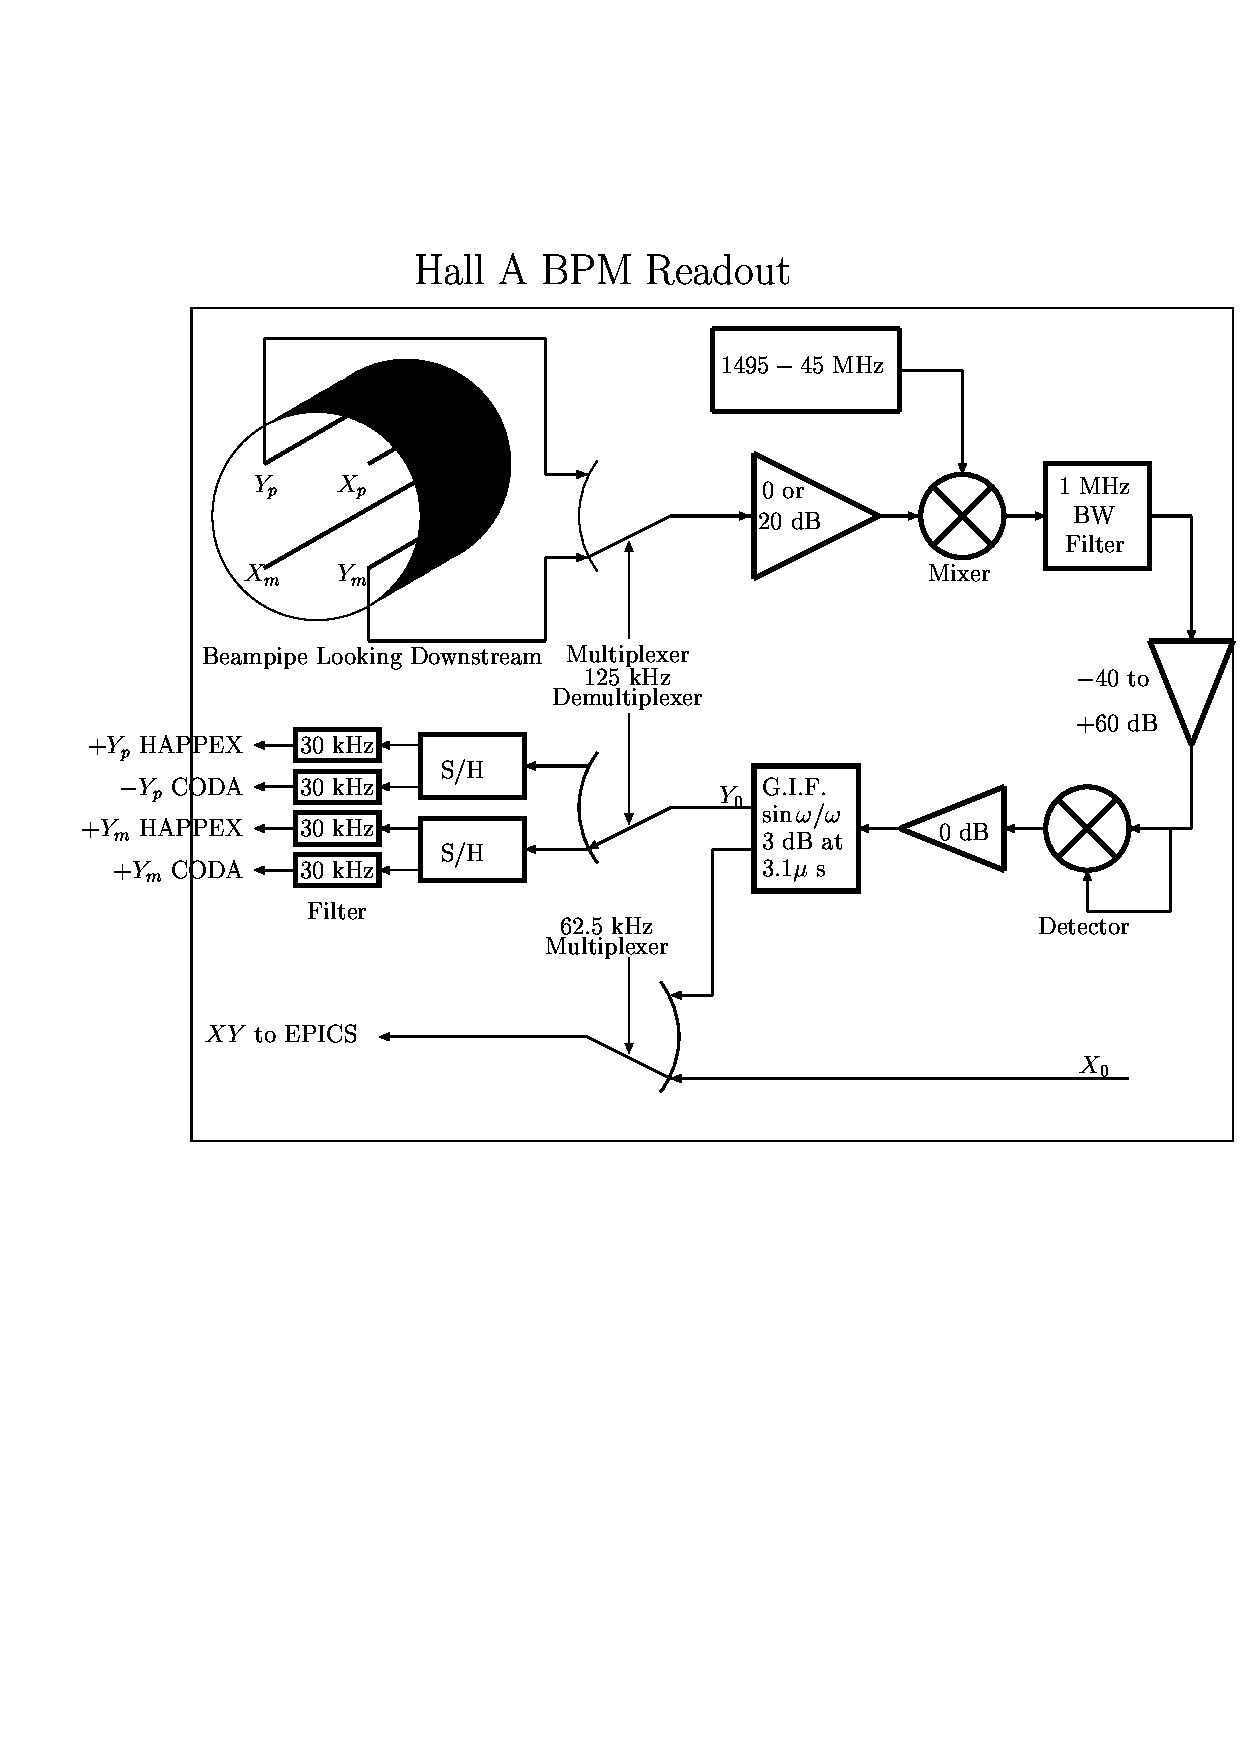
\includegraphics[angle=0,width=15cm]{BPM_fig}
{\linespread{1.}
\caption[Beamline: BPM Readout Electronics]{Schematic of the BPM readout
electronics}
\label{fig:bpmel}}
\end{center}
\end{figure}
}

1. The averaged position over 0.3 seconds is logged into the EPICS~\cite{EPICSwww} database (1 
Hz updating frequency) and injected into the datastream every 3-4 seconds, 
unsynchronized but with an orientative timestamp. From these values we can 
consider that we know the average position of the beam calculated in the EPICS 
coordinate system which is left handed.

2. Approximately once a shift (or more often if requested by the experimenters) 
a B-scope procedure ~\cite{bi:TP} can be performed using the same EPICS electronics 
which then gives the peak-to-peak variation of the beam.

3. Event-by-event information from the BPMs are recorded in the CODA datastream
from each of the 8 BPM antennas (2x4) from which the position of the beam can be 
reconstructed. However, these raw values belong to a parallel electronics chain 
whose constants have to be retrieved by calibrations to the EPICS or scanner 
data. 

\subsection{Beam Exit Channel}

After the target vacuum chamber, which was built by
the University of Virginia, there is an exit beam pipe which 
transfers the scattered beam onto the dump tunnel under vacuum. This exit beam 
pipe is made of a thin walled aluminum spiral corrugated pipe of welded 
construction. The largest diameter is 36 inches with a 0.164 inches wall 
thickness and the smallest diameter is 6 inches with a 0.042 inches wall 
thickness. The whole assembly is rather light (approximately 800 kg) and is 
supported by H shaped adjustable stands. To prevent possible linear collapse 
of the larger diameter sections under vacuum load, four aluminum channels of 
total cross-sectional area of 3'' are welded to its side. A vacuum of 
10$^{-5}$ Torr is maintained with a turbomolecular pump. The exit face of this 
pipe has a 12'' port and is connected to the diffuser with a Beryllium 
window.

}

\section{ Machine/Beamline protection system}
\label{sec:beam-fsd}

The MPS~\cite{MPScebaf} system is composed of the Fast Shutdown System (FSD), Beam Loss 
Monitor (BLM), and gun control system.

The FSD system is a network of permissive signals which terminate at the 
electron gun and chopper 1. The permissive to the gun and chopper
1 may be inhibited by any device connected to an FSD mode. Devices connected to the 
FSD system include vacuum valves, RF systems, Beam loss systems, beam current 
monitors, beam dumps, and particular to Hall A, the target motion mechanism 
and the raster (value and derivative).

The gun control system includes software program which monitors beam 
operating conditions and the state of the FSD and BLM systems. the program 
will warn the operators if a potential for beam damage exists. Potential for 
damage exists when running high average current beam, when FSD nodes are 
masked and when the beam power approaches the operating envelope limits for a 
specific beam dump.

\clearpage
\begin{safetyen}{10}{10}
\section{Safety Information}
\end{safetyen}
}
%
% Information for the ESAD
%

\begin{safetyen}{0}{0}

The beamline in the Hall provide the interface between the CEBAF accelerator
and the experimental hall.   All work on the beamline must be coordinated 
with both physics division and accelerator division; in order to ensure
safe and reliable transport of the electron beam to the dump.

\subsection{Hazards and Mitigations}

All magnets (dipoles, quadrupoles, sextupoles, beam correctors) and beam 
diagnostic devices (BPMs, scanners, Beam Loss Monitor, viewers) necessary for 
the transport of the beam are controlled by Machine Control Center (MCC) 
through EPICS~\cite{EPICSwww}, except for special elements which are addressed in the 
subsequent sections. The detailed safety operational procedures for the Hall 
A beamline should be essentially the same as the one for the CEBAF machine 
and beamline.\\ 

  
\noindent{}Personnel who need to work near or around the beamline should keep in mind the potential hazards:
\begin{itemize}
  \item Radiation ``Hot Spots'' - marked by ARM or RadCon personnel,
  \item Vacuum in the beam line tubes and other vessels,
  \item Thin windowed vacuum enclosers (e.g. the scattering chamber),
  \item Electric power hazards in vicinity of the magnets,
  \item Magnetic field hazards in vicinity of the magnets, and
  \item Conventional hazards (fall hazard, crane hazard etc.).
\end{itemize}

The most hazardous areas along the beamline are roped off it restrict access.   
In particule the scattering chamber, with it's large
volume and thin windows requires hearing protection once it has been evacuated.   
Signs are posted by radcon for any hot spots along the beamline and
radcon must be notified before work is done in a posted area.

Some magnets, as the M{\o}ller spectrometer elements, are covered with plastic
sheets for electric safety. Any access to these magnets requires
the ``Lock and Tag'' procedure~\cite{EHScebaf} and the appropriate training,
including the equipment-specific one. \\

\noindent{}Additional safety information is available in the following documents:
\begin{list}{--}{\setlength{\itemsep}{-0.15cm}}
  \item EH\&S Manual~\cite{EHScebaf};
  \item PSS Description Document~\cite{PSScebaf}
  \item Accelerator Operations Directive~\cite{AODcebaf};
\end{list}

\subsection{Responsible Personnel}

Since the beamline requires both accelerator and physics personnal to maintain
and operate and it is very important that both groups stay in contact that any 
work on the Hall A beamline is coordinated.

\begin{namestab}{tab:beam:personnel}{Beam line: authorized personnel}{%
   Beamline physics division and accelerator divison points-of-contact.}
  \namestabheader{Hall A Physicists}
  \DouglasHiginbotham{\em 1st Contact}
  \RobertMichaels{\em 2nd Contact}
  \namestabheader{Liaisons from Accelerator Division}
  \HariAreti{..to Physics}
  \YvesRoblin{..to Hall-A}
\end{namestab}
\end{safetyen}


\newpage
\section{ Beam Position Monitors}

To determine the position and the direction of the beam on the experimental 
target point, two Beam Position Monitors (BPMs) are located at distances 7.524 m 
(IPM1H03A) and 1.286 m (IPM1H03B) upstream of the target position. 
The BPMs consist of a 4-wire antenna array of open ended thin wire striplines 
tuned to the fundamental RF frequency of 1.497 GHz of the beam ~\cite{bi:bar90}. The 
standard difference-over-sum technique is then used ~\cite{bi:HW} to determine the 
relative position of the beam to within 100 microns for currents
above 1 $\mu $A. The absolute  position of the BPMs can be calibrated with respect to the 
scanners (superharps) which are located adjacent to each of the BPMs (IHA1H03A 
at 7.353 m and IHA1H03B at 1.122 m upstream of the target). The schematic of the 
readout electronics is shown in Figure ~\ref{fig:bpmel}. The
position information from the 
BPMs can be recorded in three different ways:

\begin{figure}
\begin{center}
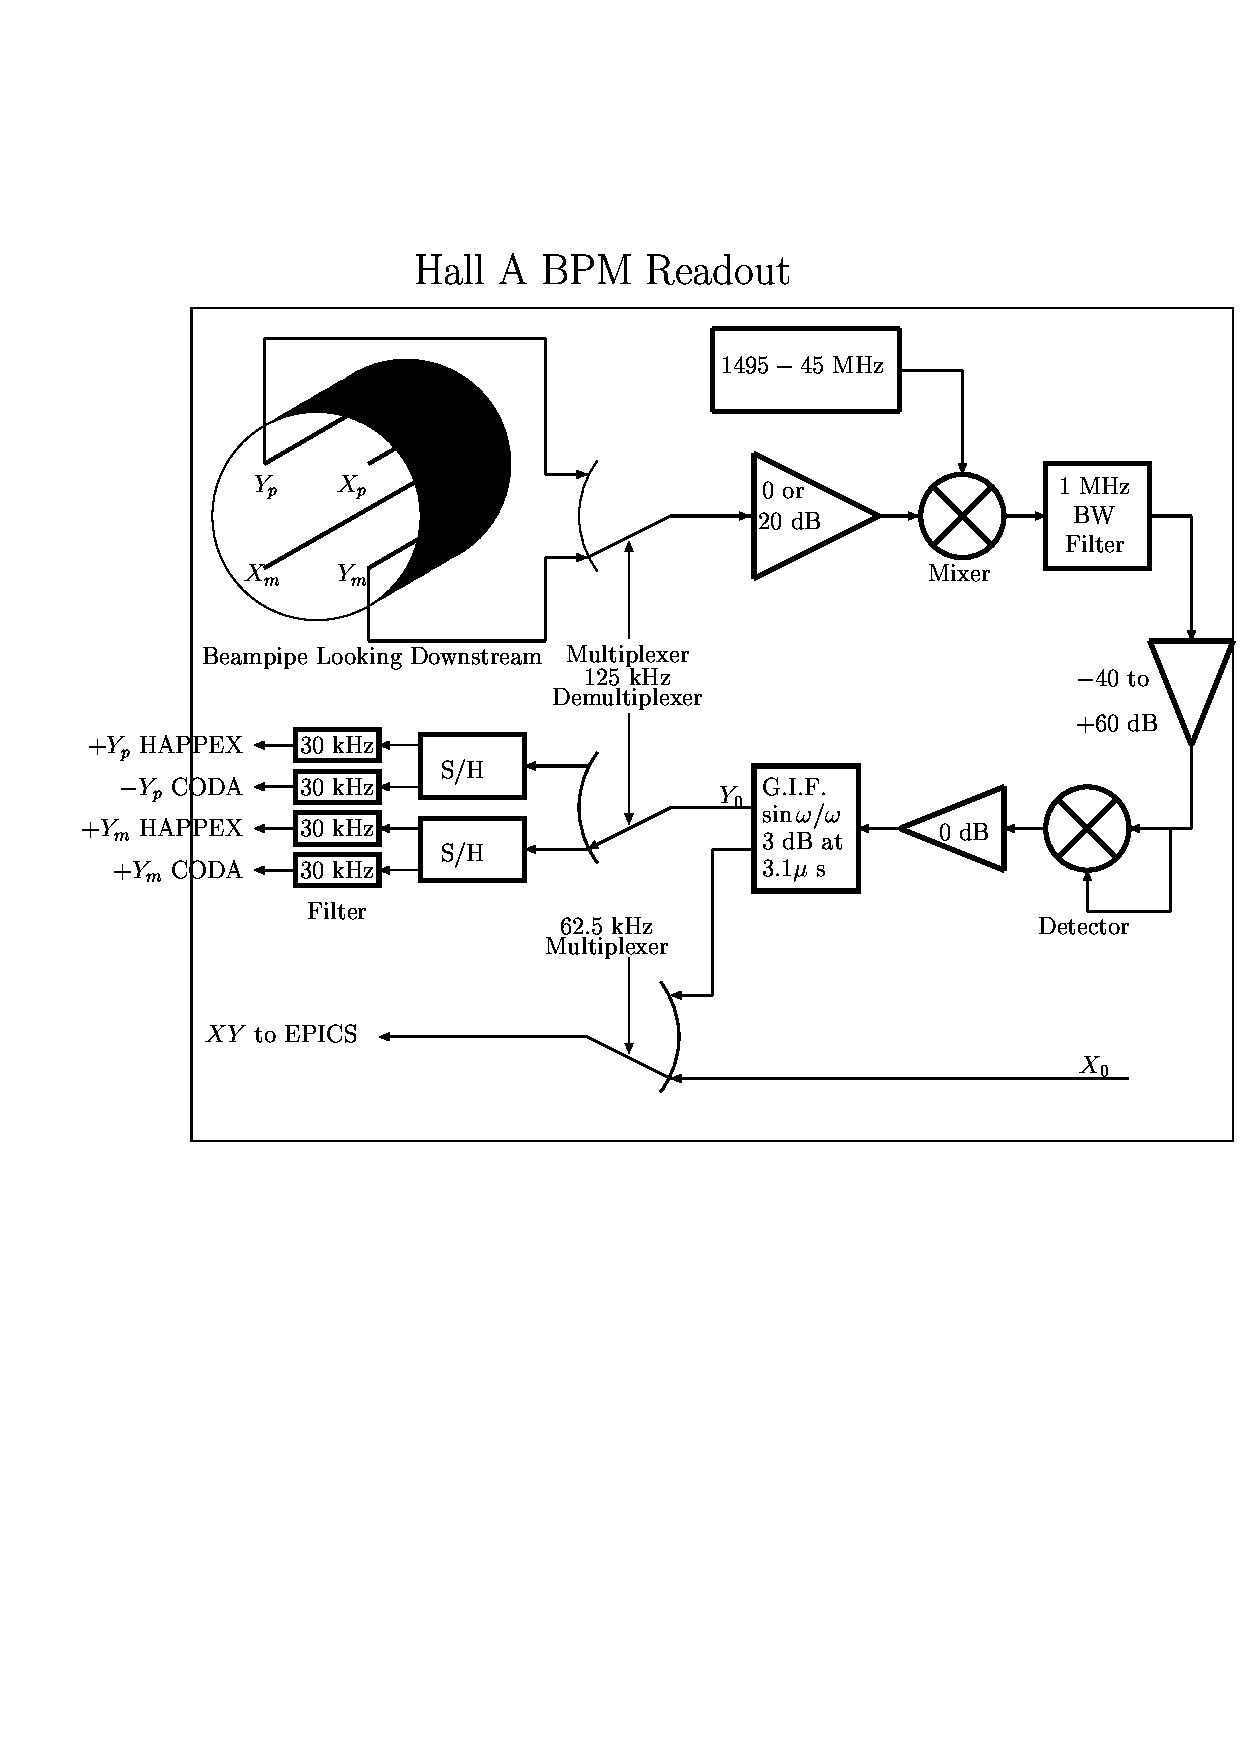
\includegraphics[angle=0,width=15cm]{BPM_fig}
{\linespread{1.}
\caption[Beamline: BPM Readout Electronics]{Schematic of the BPM readout
electronics}
\label{fig:bpmel}}
\end{center}
\end{figure}

\vskip 0.5cm

1. The averaged position over 0.3 seconds is logged into the EPICS database (1 
Hz updating frequency) and injected into the datastream every 3-4 seconds, 
unsynchronized but with an orientative timestamp. From these values we can 
consider that we know the average position of the beam calculated in the EPICS 
coordinate system which is left handed.

\vskip 0.5cm

2. Approximately once a shift (or more often if requested by the experimenters) 
a B-scope procedure ~\cite{bi:TP} can be performed using the same EPICS electronics 
which then gives the peak-to-peak variation of the beam.

\vskip 0.5cm

3. Event-by-event information from the BPMs are recorded in the CODA datastream
from each of the 8 BPM antennas (2x4) from which the position of the beam can be 
reconstructed. However, these raw values belong to a parallel electronics chain 
whose constants have to be retrieved by calibrations to the EPICS or scanner 
data. 


%\begin{thebibliography}{99}
%\bibitem{bi:bar90} W. Barry et al., CEBAF-PR-90-009 (1990).
%\bibitem{bi:HW} C. Hyde-Wright et al., Beam Position Studies for E93050 and priv. comm..
%\bibitem{bi:TP} T. Powers, priv.  comm.. 
%\end{thebibliography}
% ===========  CVS info
% $Header: /group/halla/analysis/cvs/tex/osp/src/beamline/bpms.tex,v 1.1 2003/06/05 17:28:32 gen Exp $
% $Id: bpms.tex,v 1.1 2003/06/05 17:28:32 gen Exp $
% $Author: gen $
% $Date: 2003/06/05 17:28:32 $
% $Name:  $
% $Locker:  $
% $Log: bpms.tex,v $
% Revision 1.1  2003/06/05 17:28:32  gen
% Initial revision
%

\newpage
\section[Beam Current Measurement]{Beam Current Measurement
\footnote{
  $CVS~revision~ $Id: bcm.tex,v 1.5 2003/12/13 06:23:37 gen Exp $ $
}
\footnote{Authors: A.Saha \email{saha@jlab.org}}
}

The Beam Current Monitor (BCM) is designed for stable, low noise, non-intercepting 
beam current measurements. It consists of an Unser monitor, two rf cavities, 
the electronics and a data acquisition system. The cavities and the Unser monitor 
are enclosed in a box to improve magnetic shielding and temperature stabilization.
The box is located 25 m upstream of the target. You can recognize it as a grey 
object on the stands, about 2 m downstream from where the beam enters the 
hall. 

The DC 200 down-converters and the Unser front end electronics are located in Hall 
A. The temperature controller, the Unser back end electronics and its calibration 
current source, cavity's RF unit (housing the RMS-to-DC converter board) and all 
multi-meters, VME crate and computers are located in Hall A control room.

\infolevone{
\subsection{ System Layout}

The schematic diagram of the BCM system is presented in
Fig.~\ref{fig:halla_bcm}.
\begin{figure}[htp]
\begin{center}
\includegraphics[angle=0,width=0.9\textwidth,clip]{habcm_r}
{\linespread{1.}
\caption[Beam Current Measurement: Schematic]{Schematic of the Hall A beam
current measurement system.}
\label{fig:halla_bcm}}
\end{center}
\end{figure}

The Unser monitor is a Parametric Current Transformer designed for non-destructive 
beam current measurement and providing an absolute reference. The monitor is 
calibrated by passing a known current through a wire inside the beam pipe and has a 
nominal output of 4 mV/$\mu $A. It requires extensive magnetic shielding and 
temperature stabilization to reduce noise and zero drift. As the Unser monitor's 
output signal drifts significantly on a time scale of several minutes, it cannot be 
used to continuously monitor the beam current. However, this drift is measured 
during the calibration runs (by taking a zero current reading) and removed in 
calibrating the cavities.  The more stable cavities are then used to determine the 
beam current and charge for each run. We also use the OLO2 Cavity Monitor and the 
Faraday Cup 2 at the Injector section to provide an absolute reference during 
calibration runs.

The two resonant rf cavity monitors on either side of the Unser Monitor are 
stainless steel cylindrical high Q ($\sim 3000$) waveguides which are tuned to the 
frequency of the beam (1.497 GHz) resulting in voltage levels at their   outputs 
which are proportional to the beam current. Each of the rf output signals from the 
two cavities are split into two parts. One part of the signal is  converted to 10 
kHz signals (by the ``downconverters'') and fed into an RMS-to-DC converter board 
consisting of a 50 kHz bandpass filter to  eliminate noise, amplified and split to 
two sets of outputs, which after further processing are recorded in the data 
stream. These two paths to the data stream (leading to the sampled and integrated
data ) will now be described. (The other part of the split signal is downconverted 
to 1 MHz signals and represents the old system (pre Jan 99). Only the HAPPEX 
collaboration presently uses these signals.)

For the sampled (or EPICS~\cite{EPICSwww} or Slow) data, one of the amplifier outputs is sent to a 
high precision digital AC voltmeter (HP 3458A). Each second this device provides 
a digital output which represents the  RMS average of the input signal during that 
second.  The resulting number is  proportional to the beam charge accumulated 
during the corresponding second (or, equivalently, the average  beam current  for 
that second). Signals from both cavity's multi-meters, as well as from the 
multi-meter connected to the Unser, are transported through GPIB ports to the HAC 
computer where they are recorded every 1 to 2 seconds via the data-logging process 
which is described in the calibration procedure. They are also sent through EPICS 
to CODA and the data stream where they are recorded at  quasi-regular intervals, 
typically every two to five  seconds.

For the integrated (or VTOF or Fast) data, the other amplifier output is sent to an 
RMS-to-DC converter which   produces  an analog DC  voltage  level. This level 
drives a Voltage-To-Frequency (VTOF) converter whose output frequency is  
proportional to the  input DC voltage level. These signals are then fed to Fastbus  
scalers and are finally injected into the data stream along  with the other scaler 
information.  These scalers simply accumulate during  the run, resulting  in a 
number which is proportional to the time integrated voltage level and therefore 
more accurately represents the true integral of the current and hence the total 
beam charge. The regular RMS to DC output is linear for currents
from about 5 $\mu$A to somewhere well above 200 $\mu$A.
 Since it is non-linear at the lower 
currents, we have introduced a set of amplifiers with differing gains (x3 and x10) 
allowing the non-linear region to be extended to lower currents at the expense of 
saturation at the very high currents. Hence there are 3 signals coming 
from each BCM (Upx1, Upx3, Upx10, Dnx1, Dnx3, Dnx10). All 6 signals are fed 
to scaler inputs of each spectrometer (E-arm and H-arm) . Hence we have a 
redundancy of 12 scaler outputs for determining the charge during a run. During 
calibration runs we calibrate each of these scaler outputs.   
}

\begin{safetyen}{10}{10}
\subsection{ Authorized Personnel}
\end{safetyen}

All Hall A members are authorized to take BCM calibration data using the Standard 
Non-Invasive Hall A BCM Calibration Procedure. The extended calibration procedures 
involving the Faraday Cup 2 and the OLO2 monitor at the Injector are presently 
performed by A. Saha. 

\vskip 0.2cm

The Accelerator AES group performs the maintenance of the BCM monitors. These 
include:

\begin{tabular}{l l}
1. The Unser calibration. & Every 3 months \\
2. Resonant Cavities Tuning. & Every Downtime \\
3. Multi-meters Autocalibration. & Every Downtime \\
4. Connectors Cleaning. &  Every year \\
5. Unser Keithley Current Source. & Calibration Yearly \\
6. Digital Multi-meters HP3458A and HP 34401A. & Calibration Yearly\\   
\end{tabular}

System Contacts are shown in Table~\ref{tab:BCM:personnel}.
\begin{namestab}{tab:BCM:personnel}{BCM: authorized personnel}{%
   Beam Current Monitor: authorized personnel}
  \ArunSaha{\em Contact}
  \JohnMusson{Accel. expert}
\end{namestab}
%Jean-Claude Denard -x 7555




% ===========  CVS info
% $Header: /group/halla/analysis/cvs/tex/osp/src/beamline/bcm.tex,v 1.5 2003/12/13 06:23:37 gen Exp $
% $Id: bcm.tex,v 1.5 2003/12/13 06:23:37 gen Exp $
% $Author: gen $
% $Date: 2003/12/13 06:23:37 $
% $Name:  $
% $Locker:  $
% $Log: bcm.tex,v $
% Revision 1.5  2003/12/13 06:23:37  gen
% Septum added. Name tables. Polishing
%
% Revision 1.4  2003/12/05 05:48:30  gen
% Polishing
%
% Revision 1.3  2003/06/06 15:19:02  gen
% Revision printout changed
%
% Revision 1.2  2003/06/05 23:29:59  gen
% Revision ID is printed in TeX
%
% Revision 1.1.1.1  2003/06/05 17:28:32  gen
% Imported from /home/gen/tex/OSP
%
%  Revision parameters to appear on the output

\newpage
\section[Fast Raster]{Fast Raster
\footnote{Authors: R.~Michaels \email{rom@jlab.org}}
}


The beam is rastered on target with an amplitude of
several millimeters at 25 kHz to prevent overheating.  
The raster is a set of four of air-core dipoles located
approximately 23 m upstream of the target. 
Two dipoles are for horizontal (X) motion and
another two for vertical (Y).  During the 6 GeV era
there was only one pair of X and Y, but we have doubled
the raster to account for the energy increase to 11 GeV.
The arrangement along the beamline along the 
direction of the beam will be XXYY.

For a typical 40A current in the raster coils, the
deflection by one pair (e.g. the X direction) of coils, 
in radians, is $\theta = 1.94 \times 10^{-3}/ E$
where $E$ is the electron's energy in GeV.
For example, at $E = 6$ GeV, a 0.32 mrad deflection is achieved.
Projected onto the target (about 21 m away) this is a $\pm$ 6.8 mm
excursion {\it if} there were no other magnetic fields 
between the raster and the target; however, there are quadrupoles
which change this depending on the beam tune.

Since 2003 we've used the triangle-wave 
raster pattern designed by Chen Yan.  
This achieves a very uniform rectangular
density distribution of beam on the target 
by moving the beam with a time-varying dipole
magnetic field whose waveform is triangular
with very little dwell time at the peaks.  
The electronics design is an ``H-bridge''
in which switches are opened and closed 
at 25 kHz, to switch between two directions 
of current (100 A peak-to-peak) 
through the raster coils.

Three new features during the 12-GeV era are 
1) the driver of the H-bridge electronics is now
an Agilent model 33522A waveform generator; and
2) The two X are synchronized with each other, and
the two Y are synchronized.  This makes the kicks
add and allows us to accomodate the higher energy
of the beam; and 3) The entire raster can
be synchronized to an external 10 MHz wavetrain
supplied by the polarized injector electronics.
This makes the nominal 25 kHz an exact multiple of
the helicity-flip rate, which achieves a cancellation
of raster noise, important for parity-violation 
experiments only.
The syncrhronization of the pairs of X and Y are
accurate to within a few nsec.

For most users, these three new features will not be
noticeable and the raster will appear to function
the same as during the 6 GeV running.
A user can view the 
status of the raster in the
EPICS overview screen called ``General Accelerator
Parameters'' where the set-point for the radius amplitude
and the readback of the peak-current in the raster are displayed.

Control of the raster is done by first asking the MCC
operators to set up the raster for a particular size
typically 2 mm square.
The control software assumes a field-free region between
the raster and the target, so it is only approximately
correct because there are several quadrupoles in this region.
It is important to check the raster spot size and
make adjustments if necessary.  The adjustment is made
by asking MCC to change the size and noting the 
linear relationship between what their software says
the size is and the actual size.
Relatively small independent adjustments to the 
gains on the X and the Y raster
coils are available in the middle room of the hall A
counting room using the ``PGA Controller'' knobs;
however, it is not recommended to touch these.
Near these knobs is also located an oscilloscope X-Y trace
of the current in the raster.  A fast shutdown (FSD) shuts
the beam down within 0.1 msec if the raster fails, thus
affording some protection of the target.

{\it NOTE:  If you are unsure of the status of the raster,
measure the spot size with very low current ($\le 2 \mu$A) or with
the target out of the beam.}  It would be a mistake
to check the beam spot size with high current on target; by
the time you check it, the target may already be destroyed.
The rastered beam spot on target can be checked with
plots in the ROOT analyzer or by 
using the stand alone code called \mycomp{spot},
also called \mycomp{raster}.
For more details on usage, type \mycomp{spot -h} (help)
on the ADAQ computers.

Regarding the BPM measurements, it should be noted that 
the stripline BPMs displayed by \mycomp{spot} have a high-frequency 
cutoff of approximately 30 kHz.  Since the raster frequency is 25 kHz
the plot of the amplitude distribution shows spikes at the 
limits of the orbit, instead of a flat distribution.  The scale
factor between what is seen in \mycomp{spot} and the real width of the beam
is $\sim 1.5$, i.e. the beam is 1.5 times bigger than the naive
reading of the \mycomp{spot} distribution.



\newpage
% Updated Comments Dec. 2
\infolevone{
\chapter[Arc Energy Measurement]{Arc Energy Measurement
\footnote{Authors: D. Higinbotham \email{doug@jlab.org}}
}
}

\infoleveqnull{
\section{Arc Energy Measurement}
\subsection{Overview}
In order to determine the integral field of the eight dipoles that lead to Hall A, and 
in turn determine the beam energy, a nineth dipole wired in series with the rest is 
located in a special shed near the hall A counting house.
}

\infolevone{
The ARC energy measurement is under EPICS~\cite{EPICSwww} control through 
a MEDM~\cite{MEDMwww} display. Two
independent control systems are used: the beam bend angle measurement through
the arc ("scanners") and the field integral of
the arc ("integral"). To measure the energy: 

\begin{itemize}
\item perform several angle measurements 
\item perform an integral measurement 
\item analyze the integral measurement and note the value of the arc field 
integral 
\item analyze the angle measurements, average the results (proposed by the 
software),
then ask for the energy calculation, enter the above arc field integral and
you will get the beam energy computed from the average angle. 
\end{itemize}

\section{Summary of ARC operations }

Six scanners of the same type, called ``ARC scanner'' and labelled
from scanner \#1 to \#6, are installed on the Hall-A beamline. Scanners \#1
to \#4 are used for the ARC energy measurement and they are located on the Hall-A
arc: \#1 [1HA1C07A] and \#2 [1HA1C07B] just upstream of the arc, in the BSY, and 
\#3 
[1HA1C18A] and \#4 [1HA1C18B] in the Hall-A
tunnel, just upstream the Compton polarimeter. Scanners \#5 [1HA1H03A] and \#6 
[1HA1H03B] 
are located
between the Moller and the target to control the beam geometry on the target
and their use will not be discussed here. 

Procedure for running a harp scan is described elsewhere\footnote{
Harp scan procedure \url{http://hallaweb.jlab.org/equipment/beam/harp_halla/harp.html}.}

Each scanner has a motor/ball-screw/shaft-encoder/vacuum-penetrator system moving
accurately a set of 3 tungsten wires through the beam. Each time a wire crosses
the beam a PMT located a few meters downstream records a signal due to the 
electromagnetic
shower induced by the beam in the wire. Both forward and backward passes are
recorded. The motion is a horizontal translation and, for a forward pass: 

-the translation is from beam left to beam right, 

-the two first wire crossing the beam are at 45deg from the vertical, 

-the third wire, which is the only important for the ARC energy measurement,
is vertical. 

Recording, during the scan, the scanner position and the PMT output voltage
allows us to determine the beam position at each scanner location. Then, using
calibration data not detailed here, we deduce the net beam bend angle through
the arc. This result measured in dispersive arc tuning, along with the field
integral of the arc dipoles, provides an accurate determination of the beam
energy. 

\vspace{0.3cm}

\section{Summary of field integral }

The purpose is to measure absolutely the straight field integral of a 
"BA"
3m long dipole, called the "9th dipole" and located in the
"Dipole Shed". It is of the same type as the 8 arc dipoles
and is powered in series with them. 

The ARC integral setup is basically made of a 3m long plate (the 
"probe")
which is able to move inside the 9th dipole gap along the beam axis and carrying 
two
field measurement devices: a pair of pick-up coils connected in series and a
set of NMR probes. The coils are on both ends of the probe and the NMRs close
to the center. 

-at the "upstream" probe position, the 
"downstream"
coil is close to the dipole center, the "upstream" is outside
the dipole and the NMRs at one end of the dipole: 

Door$<-$-- ....................$<-$-------DIPOLE-----$--->$ 

.............$<-$-------PROBE------$--->$ 

-at the "central" probe position, each coil is at one end
of the 3m long dipole and the NMRs close to the dipole center: 

Door$<-$-- ...................$<-$-------DIPOLE-----$--->$ 

..................................$<-$-------PROBE------$--->$ 

-at the "downstream" probe position, the 
"upstream"
coil is close to the dipole center, the "downstream" is outside
the dipole and the NMRs at one end of the dipole: 

Door$<-$-- ...................$<-$-------DIPOLE-----$--->$ 

....................................................$<-$-------PROBE------$--->$ 

We call upstream the position where the probe is the closest to the shed access
door. Among the 3 above positions, the only one where the NMR can lock on the 
dipole
field is the central one as in the extreme position of the probe, the field 
homogeneity
is not sufficient. The probe position is controlled by a linear encoder. The
Z axis refers to the "beam" direction, increasing from upstream
to downstream. We use three kinds of "Z": 

-Zm to locate a point inside the magnet. The dipole center is at Zm=0 and the
yoke ends at +-1500.mm 

-Zp to locate a point inside the probe. The probe center is at Zp=0. Each of
the 4 NMR probes has a Zp given in the file "magnet.dir".
At a temperature of 21C, the coils are at Zp=+-1519.815mm (from magnet.dir) 

-Zd to refer to a displacement of the probe w.r.t. the dipole. Zd=0 refers to
the upstream (home) position of the probe. The integral measurement is performed
from Zd=0.000mm (1st PDI trigger) to Zd=3199.000mm (last PDI trigger), for forward
pass. Zd is given by the display (at the top of the rack) or by the master screen
("OUT"). 

The relationship between Zm, Zp and Zd is: 

Zd-Zm+Zp=C 

where C is a constant given in magnet.dir (C=1604.000 nomin.). Example of use:
to have the probe center at the dipole center, one must set Zd=1604.000mm (set
Zm=0 and Zp=0 in the above formula, and solve for Zd) 

The integral measurement sequence is the following: 

-from the current position (a priori arbitrary) move the probe upstream, up
to a limit (optic) switch. 

-move downstream by a few mm to cross the encoder index (encoder initialization) 

-move to the central position to measure the central field by NMR, the system
checks if the NMR locks and if the reading is stable, it will be the 
"before"
field 

-move back to upstream position 

-move to downstream position while integrating the flux through the coil system,
this measurement will be called the "forward" integral (duration
\( \sim  \) 7s) 

-move back to upstream position while integrating the flux through the coil
system, this measurement will be called the "backward" integral
(duration \( \sim  \)7s) 

-move to the central position to measure the central field by NMR, the system
checks if the NMR locks and if the reading is stable, it will be the 
"after"
field. 

In addition to the central field, 4 probe temperatures, a local excitation current
measurement, the setting of the dipoles P.S, the readback of the dipoles P.S
and the probe position at NMR measurement time are recorded 
"before"
and "after". 

To perform an integral field measurement: 

1-check if the system works (see "details on integral system 
check"
below) 

2-run the above integral sequence (see "details on integral run"
below) 

3-fix the error(s) if any (see "details on integral errors"
below) 

4-save the data in a file (see "details on integral data save"
below) 

5-analyze the data  


\section{Details on integral run }

To run the integral measurement sequence, call the 
\mycomp{arc\_integral.adl}
medm screen, then: 

-push "start" to start the full sequence 

-look at the results displayed: 

-after the "before" NMR measurement: the 
"before"
data set 

-after the "forward" integral pass: the forward velocity profile
and the forward voltage-after-gain profile 

-after the "backward" integral pass: the backward velocity
profile and the backward voltage-after-gain profile 

-after the "after" NMR measurement: the 
"after"
data set 

-if "BAD NMR" or "PDI saturation" flags
are set, or if something is obviously wrong in the data or plots, call expert. 

-data are ready to be saved (see "Details on integral data save"
below) 


\section{Details on temperatures }

The AC system of the shed is made of two cooling units, a heating unit and a
controller connected to two temperature sensors : one located in the shed and
one located in the BSY. This system is programmed in such a way that the 
temperature
of the shed follows the BSY temperature within +-2C. The BSY temperature can
be anywhere in the 18C to 35C range, regardless of the season. The BSY 
temperature
and the shed temperature are given (in F) by a display panel located close to
the workstation, on the wall. The AC system can be set in manual control by
turning from "auto" to "manual" a set of
switches controlling the cooling units and the heater unit. These switch boxes
are located on the shed wall. If the shed temperature is above 34.4C (94F),
call the crew chief (the electronics can be damaged) and cool down the shed in manual
AC mode. The 4 temperature sensors of the probe are labelled Tx+z+, Tx+z-, Tx-z+,
Tx-z- depending on their position w.r.t. the frame. 

Both "x+" sensors are on the probe edge which is inside the
dipole gap and both "x-" sensors on the opposite edge which
is outside the dipole gap. Both "z-" sensors are at 1/4 of
the long dimension of the probe and both z+ at 3/4 of this length. The average
of the 4 temperatures is used by the analysis program to correct the coil distance
from the thermal expansion of the probe, so it is important to make sure that
the 4 sensors are working well. The user can just make sure that the temperatures
displayed in \mycomp{arc-master.adl} or recorded in 
\mycomp{arc-integral.adl}
are realistic. In \mycomp{arc-integral.adl} they are given in the
order: Tx+z-, Tx+z+, Tx-z-, Tx-z+ Tx-z- and Tx-z+ should be close to the shed
temperature. Tx+z- and Tx+z+ depend on the probe position, as the gap (iron
yoke) is warmer than the shed and the dipole coil (at both ends of the dipole)
is warmer than the iron yoke. For a probe in a central position for more than
about one hour, the Tx+z- and Tx+z+ sensors should give the yoke temperature,
i.e the shed temperature plus 0. to 5.C, depending on the current, LCW temperature
and the magnet/shed temperature history. The 4 temperatures are also displayed
inside the shed, on the electronics rack. These values are digitized by separate
ADCs, so they may differ from the remote values by \( \sim  \)0.1C. 
}

\begin{safetyen}{10}{10}
\infolevone{\section{Shed access and safety }}

Due to the the dipole magnet and motion system, the access to the shed is limited to authorized
persons which are listed in the ESAD and listed below. To be added to the list, 
contact Douglas Higinbotham.
The standard
operation mode of the integral measurement setup is the remote mode, through
the network, from the counting house.
\end{safetyen}

\begin{safetyen}{10}{10}
\infolevone{\section{List of Authorized Personnel for Shed Access}}
\infoleveqnull{\subsection{List of Authorized Personnel for Shed Access}}
\end{safetyen}
\begin{namestab}{tab:arc:personnel}{Arc Energy Measurement: authorized personnel}{%
                 Arc Energy Measurement: authorized personnel}
  \namestabheader{Hall A Personnel}
  \DouglasHiginbotham{\em Contact}
  \namestabheader{Accelerator Personnel}
  \MichaelTiefenback{}
  \YvesRoblin{}
  \RickGonzales{}
  \BillMerz{}
  \MarkAugustine{}
  \HariAreti{}
  \PeteFrancis{}
  \ScottHiggins{}
  \DavidSeidman{}
  \RonLauze{}
  \TonyDay{}
  \ChristopherCurtis{Alignment group}
  \namestabheader{CEA - Saclay experts}
  \PascalVernin{}
  \ChristianVeyssiere{}
  \FrancoisGougnaud{}
  \JacquesMarroncle{}
\end{namestab}



\newpage
\infolevone{
\chapter[Target Chamber]{Target Chamber
\label{sec:target_chamb}
\footnote{
  $CVS~revision~ $Id: tgtcham.tex,v 1.11 2005/04/04 22:27:25 gen Exp $ $
}
\footnote{Authors: ?? \email{??@jlab.org}}
}

The cryo-targets and the waterfall targets 
(see Sec.~\ref{sec:targets-overv}) 
are contained in a special target chamber which is a large 
evacuated  multistaged can. So far, three chambers have been designed:
\begin{list}{\arabic{enumi}.~}{\usecounter{enumi}\setlength{\itemsep}{-0.15cm}}
  \item a chamber used up to 2003;
  \item a chamber designed for use with septum magnets, starting in 2003;
  \item a chamber designed for use with the BigBite spectrometer.
%\footnote{
%        No yet manufactured by Dec,2003.}.
\end{list}

Here, chamber 1 is described. Chambers 2 and 3 are only different in 
size and slightly in shape. The safety considerations fully apply to chambers 2 and 3.
The chamber was designed to isolate the beam line vacuum from  each
HRS so that each HRS could rotate
around the target without vacuum coupling and without jeopardizing
certain desired kinematic and acceptance  specifications of 
both high resolution spectrometers
needed for approved experiments.  It  was also designed to simultaneously
 contain a liquid or gas target and an array of water cooled thin
 metallic foils, both remotely controlled and also be adaptable for
the waterfall target. The desired kinematic specifications that were
 considered included momentum and energy resolution in both arms,
 angular range of spectrometers, angular acceptance, and luminosity.
The chamber vacuum is isolated from the  HRS by using thin aluminum foils. 

The target chamber is designed so that
each spectrometer will have continuous coverage in the standard tune from
$\theta_{min}=$12.54$^\circ$ to $\theta_{max}=$165$^\circ$.
The aluminum window is 6~$in$ high and 0.016~$in$ thick made of 5052 H34 aluminum foil.
The foil forms regularly spaced vertical ridges when
placed under load. The window had an inter-ridge
spacing of 3 inches.
If the window is treated as a collection
of smaller rectangular windows which have the full vertical height
of 6 inches and the inter-ridge spacing as a width,
then stress formulas predict that the 0.016 $in$
material would reach ultimate stress at a pressure higher than 35 PSID
(for both over-pressure and under-pressure). 
There is a gate valve between the 
scattering chamber and the beam entrance (exit) 
pipe. Both 
valves will be closed automatically in the
event that the chamber vacuum begins to rise and an FSD will be caused
( this is done via a relay output of the scattering
chamber vacuum gauge). If either valve is closed an FSD will result.

The target chamber is supported by a 24 $in$ diameter pivot post
secured in concrete, rising about 93.6 $in$ above the Hall A cement floor.
The Hall A target chamber
consists of an aluminum middle ring, a stainless steel base ring,
each with a 41.0 $in$ inner diameter,
and a stainless steel cylindrical top hat with 40 $in$ inner diameter
to enclose the cryotarget and secure the cryogenic connections.

When the scattering chamber is under vacuum, there is a potential
danger of window rupture.
The loud noise from the rupture could hurt
one's ears if not protected. Therefore when the chamber is under vacuum,
protective covers are put on if possible. These must be taken off
for data taking. For restricted access, the protective cover is required
to be on when the chamber is under vacuum. Before switching from controlled
access to restricted access, the protective cover is required to be installed.
Anytime that the scattering chamber
is under vacuum, the pivot area is enclosed in a rope or tape barrier
and a warning sign is posted.
Hearing protection is required in the enclosed area.

\infolevone{
	The aluminum ring with an outer diameter of 45.0 $in$ and
wall thickness 2.0 $in$  is necessary for a sturdy support structure and
to permit machining of the outside surface to accommodate
the flanges for fixed and sliding seals mounted on
opposite sides of the ring that vacuum connect the chamber to each HRS.
The height of the aluminum ring shown is 36.0 $in$, which is
designed to accommodate the mounting flanges.
The stainless steel base ring 
is 11.50 $in$ in height with
one pump-out 6 $in$ diameter port  and with
seven 4 $in$ viewing and electrical feed-through ports.
The base ring will also contain support mechanisms for the solid
target ladder assembly, a rotisserie for collimating slits, radiators, and
magnetic
fingers for
removing the solid target vacuum-lock can. The total height of the top
ring, middle ring, and
base ring is 93.81 $in$. This length is partly determined by our desire to
include with the cryogenic extended target a solid target vertical ladder
secured in an inverted hat through a hole in the base of the chamber.

	The base ring includes an end plate through which the
inverted hat will be adapted to fit into the large vertical pipe serving
as the pivot post for the Hall A spectrometers.

	The stainless steel cylindrical top hat  has
40.0 $in$ inner diameter, and is 0.375 $in$ thick and
46.31 $in$ high , which is necessary to permit the
cryotarget to be withdrawn and to make space available to expose the solid
targets to the electron beam.

   The 200 $\mu$A electron beam, focused to a $\sim$\(0.1\, mm\times
0.1\) mm spot and rastered $\pm$5 mm horizontally or vertically on the
target, enters through a oval hole in the middle ring which
is 2.06 $in$ wide and exits through a 1.81 $in$ hole connected to the
exit pipe.
}

\infolevone{
\section{Target Chamber - Spectrometer Coupling}

   The aluminum middle ring will support a flange on each side for each high
resolution spectrometer. Four flanges will be available: Two flanges will
contain a 6 $in$ window opening which will be covered with a thin foil
(e.g., 10 mil aluminum) .
These two flanges will be used for experiments utilizing
extended  targets that do not require optimum momentum resolution.
The other two flanges will have two fixed ports (with a 8 $in$ $\times$ 6 $in$
opening)
which will be mainly used for calibration of the spectrometers . Fixed ports are
centered at 16.11 $^\circ$ and
45 $^\circ$ for one flange and at 16.11 $^\circ$ and 90 $^\circ$ for the second
flange.

   For a point beam on target a vertical opening in the walls of the chamber
of height 57.15 cm x 0.065 x 2 = 7.43 cm is required so that the scattered
beam is within the full acceptance of the spectrometer.
If the beam is rastered on target $\pm$0.5 cm in the vertical direction,
then the opening in the outer side of the chamber must be at least 8.5 cm for
full acceptance.

From consideration of the angular range of the spectrometers in the standard
tune, the scattered beam acceptance envelope, the effects of an
extended gas target on acceptance,
and the effects of a rastered beam $\pm$ 5 mm on acceptance,
the target chamber requires a window of at least 8.5 cm
high in the aluminum ring extending from 6.33 $^\circ$ (2.48 in) from the
beam exit point to 8.83 $^\circ$ (3.47 in) from the beam entrance point on one
side and a similar window on the other side of the beam.
For future considerations (e.g., using a third arm or sliding seal) the
width of the window on the middle ring was actually constructed
to be 17.78 cm (7 $in$).

\section{Stress Analysis of the Middle Ring}

Since the middle ring has an extensive cut across the midplane on both sides as
well as
entrance and exit holes and loaded with about 25,000 lbs, calculations of the
stresses
 and deformation of  the
midplane support area of the middle ring and deflection of the window opening
were made using the finite element analysis code ANSYS . The work was conducted
by a graduate student in the Department of Civil Engineering at the
University of
Virginia and a REU student.  A scaled down model of the middle ring was
constructed and then tested by applying forces to it using the Materials Testing
Service of the Department of Transportation at the University. ANSYS was first
checked by comparing calculations of the test model deflections to the actual
data. Agreement was  within $\pm$10\%. Results of ANSYS for the target
chamber showed that the maximum deflection of the opening of the window in the
middle ring varied from 0.007 $in$ to 0.015 $in$ depending on how the
middle ring
was loaded. This was decided to be a safe limit. In the final design, several
movable
7 $in$ long, 2 $in$ diameter aluminum support rods are placed in the
window for added support. In addition, flanges defining the ports and
coupling to
the spectrometers can be added, giving additional support to the middle ring.
Compressional stresses, calculated using ANSYS assuming the middle ring was
attached to the
top hat and loaded with 25,000 lbs, were less than 3000 psi 
almost everywhere.
However, stresses over small areas rose to levels 6000 psi near the entrance
and exit holes. These calculations indicated that we did not exceed the safety
limit of 15,000 psi for aluminum. A simple model calculation shown in Appendix
A  gives the result 1434 psi, which represents some average value over the
midplane
contact area.

\section{Vacuum Pumping System}

The vacuum in the target chamber is maintained by an Alcatel ( 880 l/s)
 turbomolecular vacuum pump. The pump is connected to a 6 $in$ port in the
stainless steel ring between 130
 $^\circ \le \theta_p \le 180 ^\circ$. The vacuum pump is
fastened to a horizontal pipe connected to the chamber. The vacuum pressure in
the chamber is about $10^{-5}$ mm. An additional Alcatel pump connected
to an 8 $in$ port should be added to obtain lower vacuum. Both
pumps may be isolated
from the target chamber using gate valves which are remotely operated
from the vacuum control rack and interlocked to the FSD system.


A 2 $in$ all metal gate valve is located between the entrance flange to the
chamber and the beam profile monitor.   
 An additional gate valve is located 2 m downstream of the
 target chamber to isolate the chamber from the exit beam pipe.
}
\begin{safetyen}{10}{15}
\section{Safety Assessment}
\end{safetyen}

The scattering chamber is typically a low maintenance item but it is a vacuum
system and hence problems may occur. The day to day operations of the cryogenic
targets are managed by the Hall A Staff while major maintenance operations are
handled by the Cryogenic Target Group (Physics Division). Occasionally the
cryogenic targets experience difficulties due to failures of the End Station
Refrigerator which supplies the coolant. In these cases the Cryogenics Group
of the Accelerator Division should be contacted.

\noindent{}The target chamber may pose several hazards:

\begin{list}{\arabic{enumi}.~}{\usecounter{enumi}\setlength{\itemsep}{-0.15cm}}
  \item {\bf Rupture of vacuum windows}. This hazard is mitigated by
        lexan guards on the vacuum windows, installed by the hall technicians
        either at the beginning of a ``restricted access'' period 
        %(see Sec.\ref{sec:Access}),
        or during ``control access'', in case an access to the target chamber area is needed.
        Installation and removal of the guards is included in the technician's checklists.
        When the chamber is under vacuum, it is mandatory to use ear protection in the chamber
        vicinity. The appropriate signs must be installed by the technicians. 

  \item {\bf Induced radioactivity}. The RADCON surveyor measures the level of induced
        radiation as a part of the general survey and may declare the target area 
        as ``High Radiation Area'', installing a rope protection around\cite{RWIcebaf}. 

\end{list}

Some other safety issues are discussed in the cryo-target chapter 
(see Sec.~\ref{sec:target-cryo-safety}).
%and also in the polarized target chapter (see Sec.~\ref{sec:target-he3-general}).

\begin{safetyen}{10}{15}
\section[Authorized  Personnel]{Authorized  Personnel}
\end{safetyen}

\begin{namestab}{tab:targ_chamb:personnel}{Target chamber: authorized personnel}{%
      Target chamber: authorized personnel. ``W.B.'' stands for the white board 
      in the counting house.}
  \TechonCall{\em Contact}
  \JessieButler{}
  \DaveMeekins{Target group}
  \JianPingChen{}
\end{namestab}
}

\newpage
\infolevone{\chapter[M{\o}ller Polarimeter]{M{\o}ller Polarimeter}
\setcounter{subsection}{0}}
\infoleveqnull{\section[M{\o}ller Polarimeter]{M{\o}ller Polarimeter}}

The Hall A beam line is equipped with a M{\o}ller 
polarimeter
whose purpose is 
to measure the polarization of the electron beam delivered to the hall. 

\begin{safetyen}{0}{0}

The M{\o}ller Polarimeter system has under gone a major upgrade and an Operational Safety Proceedure (OSP)
is being written and must be reviewed before its use.

\subsection{Hazards and Mitigations}

The hazards and mitigations for this system can be found in the OSP at the end of this document. 

%\infolevone{
%Safety checklist item for this device, located at the end of the beamline section, is solely to ensure
%the beam can be tranported safetly past this system prior to it's recommisioning.
%}

\subsection{Responsible Personnel}
\label{sec:moller-pers}

This list of system experts provided in case there is any question as to the status of system.

\begin{table}[h]
\begin{center}
\begin{tabular}{|ll|l|l|l|l|r|} \hline
  \multicolumn{2}{|c|}{Name} & Dept. & \multicolumn{2}{c|}{Telephone} & 
  \multicolumn{1}{c|}{e-mail} & Comment \\ 
  \cline{4-5}
   &  &   & JLab & Pager &  & \\ 
\hline
 Javier       & Gomez           & JLab    & 7498 & 7498 & gomez@jlab.org    & Primary contact     \\ 
 Oleksandr    & Glamazdin       & Kharkov & 5441 & 5441 & glamazdi@jlab.org &  \\ 
 Viktor       & Gorbenko        & Kharkov & 5441 &   -  & gorbenko@jlab.org &  \\ 
 Roman        & Pomatsalyuk     & Kharkov & 5395 & 0001 & romanip@jlab.org  &  \\ 
\hline
\end{tabular}
\end{center}
\caption[Moller Polarimeter: authorized personnel]{
   The listed name are those who are considered system experts of the Moller Polarimeter and should be contacted
   if there is any question as to the status of the system.
}
\label{tab:moller:personnel}
\end{table}
\end{safetyen}


\newpage
}
% Compton Polarimeter
\infolevone{\chapter[Compton Polarimeter]{Compton Polarimeter}
\label{sec:compton}
\footnote{Author: S.Nanda \email{nanda@jlab.org}}
}
\infoleveqnull{\section{Compton Polarimeter}
\subsection{Overview}}


The Hall A Compton polarimeter has undergone a major upgrade and an
new operational safety proceedure (OSP) is being written and reviewed before the
Compton can be used.   The hazards and mitigations for this system can be found in 
this OSP.

\subsection{Responsible Personnel}

\begin{namestab}{tab:compton:personnel}{Compton Polarimeter: authorized personnel}{%
          Compton Polarimeter: authorized personnel}
 \SirishNanda{Primary Contact}
 \JackSegal{Secondary Contact}
\end{namestab}

\infolevone{
\subsection{Authorized Personnel}

The list
of the presently authorized personnel is given in Table~\ref{tab:compton:personnel}.
Other individuals must notify and receive permission from
the contact person (see Table~\ref{tab:compton:personnel}) to get their names
add to list.

\begin{namestab}{tab:compton:personnel}{Compton Polarimeter: authorized personnel}{%
          Compton Polarimeter: authorized personnel}
 \SirishNanda{\it Contact}
 \JackSegal{Technical}
 \JosephZhang{Optics}
 \MartialAuthier{Engineering}
 \NathalieColombel{Mechanical}
 \PascaleDeck{Electronics}
 \AlainDelbart{Optics}
 \DavidLhuillier{Analysis}
 \YvesLussignol{EPICS}
 \DamienNeyret{DAQ}
 \GerardTarte{Electronics}
 \ChristianVeyssiere{Electronics}
\end{namestab}
}



%
% Old Material
%
% \chapter[eP Beam Energy Measurement]{eP Beam Energy Measurement
\footnote{
  $CVS~revision~ $Id: ep.tex,v 1.6 2003/12/13 06:23:37 gen Exp $ $
}
\footnote{Authors: B.Reitz \email{reitz@jlab.org}}
}
\label{sec:ep}
\section {Purpose and Layout}
\label{sec:ep_purpose}

The Hall A eP system is a stand-alone device to measure the 
energy of the electron beam. It is located along the beamline
17~m upstream of the target. The beam energy $E$ is determined by measuring
the scattered electron angle $\Theta_e$ and the recoil proton angle
$\Theta_p$ in the $^1$H$(e,e'p)$ elastic reaction according to the kinematic
formula:
\begin{equation}
E = M_p \frac{\cos(\Theta_e) + \sin(\Theta_e)/\tan(\Theta_p) - 1}{1 - \cos(\Theta_p)} + O(m_e^2/E^2),
\end{equation}
in which $M_p$ denotes the mass of the proton and $m_e$ the mass of the electron.
The schematic diagram of the eP system is presented in Fig. \ref{fig:ep_layout}. 
Two identical arms, each consisting of an electron and a corresponding proton 
detector system, made up of a set of 2~x~8 silicon micro-strip detectors in the
reaction plane, are placed symmetrically with respect to the beam along the 
vertical plane. The target consists of a rotating CH$_2$ tape.
Simultaneous measurements of the beam energy with both arms result
in cancellation, to first order, of uncertainties in the knowledge of the position
and direction of the beam. 
 \begin{figure}[htb]
    \begin{center}
        \includegraphics*[angle=0,width=0.9\textwidth]{ep_layout}
    \end{center}
    \caption[eP: Layout]{
            Schematic layout of the eP energy measurement system,
            showing the arrangement of its components, the polyethylene (CH$_2$) 
            target, the Cherenkov detectors, the silicon micro-strip detectors (SSD) 
            for protons and electrons, and the scintillator detectors.
            }
    \label{fig:ep_layout} 
 \end{figure}  
%\clearpage

\infolevone{
\section{Description of Components}
\label{sec:ep_desc_comp}

\subsection{High Voltage}
\label{sec:ep_highvoltage}

The eP system is equipped with two gas Cherenkov detectors and 
altogether 18 scintillators. The high voltage for the photomultiplier
tubes of these detectors are provided by a LeCroy 1450 HV power supply,
located in the electronics racks along the beamline. The channel 
assignment and HV voltages (as of summer 2003) are given in
Table \ref{tab:ep_hv}.

\begin{table}[ht]
\begin{center}
\begin{tabular}{|l|r|l|} \hline
Channel & HV (Volts) & Detector  \\ \hline \hline
 1.2 & 2201 & S1 (bottom) \\  \hline
 1.3 & 2200 & S2 (bottom) \\  \hline
 1.4 & 1963 & S1 (top) \\  \hline
 1.5 & 1963 & S2 (top) \\  \hline
 1.8 & 1039 & S3 \\  \hline
 1.9 & 1027 & S3 \\  \hline
 2.0 & 2250 & Cherenkov  \\  \hline
 2.1 & 2250 & Cherenkov  \\  \hline
 3.0 & 1004 & S3 \\  \hline
 3.1 & 1113 & S3 \\  \hline
 3.2 & 1097 & S3 \\  \hline
 3.3 & 1144 & S3 \\  \hline
 3.4 & 1126 & S3 \\  \hline
 3.5 & 1119 & S3 \\  \hline
 3.6 & 1006 & S3 \\  \hline
 3.7 & 1112 & S3 \\  \hline
 3.8 & 1104 & S3 \\  \hline
 3.9 & 1071 & S3 \\  \hline
 3.10 & 1061 & S3 \\  \hline
 3.11 & 1051 & S3 \\  \hline
\end{tabular}
\end{center}
\caption[eP System: HV Summary]{HV connections and HV values. }
\label{tab:ep_hv}
\end{table}

\infolevtwo{
The standard way to control the high voltage is the use of the 
Hall A MEDM~\cite{MEDMwww} graphical user interface (EPICS~\cite{EPICSwww}), which is running 
on the \mycomp{hacsbc2} computer. This computer is located in the counting house,
but can also be accessed from other terminals. Usually at least one terminal 
in Hall A itself has a MEDM screen running, as well. If it is not running, log into \mycomp{hacsbc2}
as user \mycomp{hacuser}, and start the GUI with the command
\mycomp{hlamain}. A screen labeled ``Hall A Main Menu'' will appear (Fig. \ref{fig:medm-hlamain}).
Chose \mycomp{LeCroy HV}, and select \mycomp{Beamline} in the screen which will pop 
up (Fig. \ref{fig:ep_hvlecroy}). 


 \begin{figure}[bht]
    \begin{center}
        \includegraphics*[angle=0,width=6cm]{ep_lecroy}
    \end{center}
    \caption[eP: LeCroy HV Screen]{
	    Epics Menu for the LeCroy High Voltage supplies in Hall A. All slots related
            to the eP system can be accessed from the Beamline button.
            }
    \label{fig:ep_hvlecroy} 
 \end{figure}  
}

For a measurement, all HV channels defined in Table \ref{tab:ep_hv}
should be turned on. The demand voltages in these slots
(Slot 1, Slot 2 ``(e,p) \& ARC'' and Slot 3 ``Moller'') should have 
the correct preset values. 
To turn the HV on (or off), or to change the 
preset values,
press the button below the title of the slot. Another screen will pop-up,
where status and preset values can be adjusted. \infolevtwo{
(See Figs. \ref{fig:ep_hvbeamline}, \ref{fig:ep_hvslot1}, \ref{fig:ep_hvslot2}, and \ref{fig:ep_hvslot3})

\begin{figure}[bht]
    \begin{center}
        \includegraphics*[angle=0,width=0.9\textwidth]{ep_hvbeamline}
    \end{center}
    \caption[eP: Beamline HV Screen]{
	    Overview screen for the high voltage status of devices belonging to the 
            beamline instrumentation.
            }
    \label{fig:ep_hvbeamline} 
 \end{figure}  

\begin{figure}[bht]
    \begin{center}
        \includegraphics*[angle=0,width=0.9\textwidth]{ep_hvslot1}
    \end{center}
    \caption[eP: HV Screen for Slot 1]{
	    Control screen for all high voltage channels from Slot 1.
            }
    \label{fig:ep_hvslot1} 
 \end{figure}  

\begin{figure}[bht]
    \begin{center}
        \includegraphics*[angle=0,width=0.9\textwidth]{ep_hvslot2}
    \end{center}
    \caption[eP: HV Screen for Slot 2]{
	    Control screen for all high voltage channels from Slot 2.
            }
    \label{fig:ep_hvslot2} 
 \end{figure}  


 \begin{figure}[bht]
    \begin{center}
        \includegraphics*[angle=0,width=0.9\textwidth]{ep_hvslot3}
    \end{center}
    \caption[eP: HV Screen for Slot 3]{
	    Control screen for all high voltage channels from Slot 3.
            }
    \label{fig:ep_hvslot3} 
 \end{figure}
}

During a measurement, the alarm handler should be running, so that the 
operator will be informed, should one of the detectors trip. \infolevtwo{This can
also be done manually, by watching the beamline screen Fig. \ref{fig:ep_hvbeamline}.
All fields should be green and showing a voltage close to the values given
in Table \ref{tab:ep_hv}.}
If the EPICS screens are not working, there is an alternative way to 
control the HV, by connecting via telnet directly to the LeCroy 1450.
This can be done from nearly any Linux PC in the counting house with the 
command: \mycomp{$>$ telnet hatsv5 2011}.

%\clearpage

\subsection{MEDM Controls}
\label{sec:ep_medm}

\infolevtwo{
 \begin{figure}[bht]
    \begin{center}
        \includegraphics*[angle=0,width=0.3\textwidth]{ep_slow}
    \end{center}
    \caption[eP: Slow Controls Screen]{
	    EPICS main screen for the controls of the various devices in the eP system. 
            }
    \label{fig:ep_slow} 
 \end{figure} }
The target, the silicon micro-strip detectors, and the setting of the 
Cherenkov detector are controlled by an EPICS GUI \infolevtwo{(Fig. \ref{fig:ep_slow})}. 
It can be started from the ``Hall A Main Menu'' \infolevtwo{(Fig. \ref{fig:medm-hlamain})}
running on \mycomp{hacsbc2} by pressing the \mycomp{EP Energy Measure} button.
(see previous chapter, to learn how to start the ``Hall A Main Menu'' in case
it is not already running)
The controls are actually running on a VME computer \mycomp{hallasc6} 
(Bob calls this \mycomp{e-p~2}). It is located in the eP electronics 
racks along the beamline in Hall A \infolevfour{(Fig. \ref{fig:ep_pic_slow_ctrl})}. This computer
sometimes requires rebooting. \infolevtwo{ The computer is reached through 
the portserver \mycomp{hatsv5} at port 12. To reboot:\\
\\
\mycomp{$>$ telnet hatsv5 2012 \\
user: adaq\\
password: ******* \\
\\ }
if you do not see a prompt, press \mycomp{Ctrl C}.\\
\\
\mycomp{-$>$ reboot}\\
\\
wait for it to finish and then load EPICS:\\
\\
\mycomp{-$>$ $<$ epics \\
...\\
-$>$ Ctrl $]$ \\
telnet$>$ q \\
$>$\\ }

\infolevfour{
 \begin{figure}[bht]
    \begin{center}
        \includegraphics*[angle=0,width=0.75\textwidth]{ep_pic_slow_ctrl}
    \end{center}
    \caption[eP: Picture Slow Controls]{
	    VME crate containing modules for the slow controls of the eP system.
            }
    \label{fig:ep_pic_slow_ctrl} 
 \end{figure}  }
}

\infolevtwo{
\subsection{Silicon Micro-Strip Detectors}
\label{sec:ep_ssd}

There are three GUI's associated with the silicon micro-strip detectors. 
Two of them are important for everyday operations. They are labeled 
\mycomp{MicroStrip Polarization} 
and \mycomp{MX7RH Power Supply and Currents}. To operate the SSDs, pull up
the micro-strip polarization display and turn on all the bias voltages (see Fig. \ref{fig:ep_ssd_bias_control}). 
Make sure that the bias voltages are set to a reasonable value (30 Volts).
Pop up both current strip charts so that you can see when the currents 
have stabilized.
Pull up the MX7RH display and turn on all the supply's (see Fig. \ref{fig:ep_mx7_control}). 
Pop up the power supply strip charts. It takes at 
least 30 minutes for the strips to stabilize.

 \begin{figure}[bht]
    \begin{center}
        \includegraphics*[angle=0,width=0.9\textwidth]{ep_ssd_bias_control}
    \end{center}
    \caption[eP: SSD Bias Voltages Screen]{
            EPICS screen to control the bias voltages for the silicon micro-strip detectors.
            }
    \label{fig:ep_ssd_bias_control} 
 \end{figure}

 \begin{figure}[bht]
    \begin{center}
        \includegraphics*[angle=0,width=0.9\textwidth]{ep_mx7_control}
    \end{center}
    \caption[eP: MX7 Controls Screen]{
	    EPICS screen for the MX7 power supplies. 
            }
    \label{fig:ep_mx7_control} 
 \end{figure}  

%\clearpage
}

\subsection{Target}
\label{sec:ep_target}

The target of the eP system is made of a thin polyethylene (CH$_2$) tape, which 
is moving while it is in the electron beam. \infolevtwo{ To operate the target one has to
pull up the target GUI (Fig. \ref{fig:ep_target_control}). There are two controls, one to start the target moving
labeled \mycomp{Motor Control}
and another labeled \mycomp{Target Motion} to place the target in the beam. 
 \begin{figure}[bht]
    \begin{center}
        \includegraphics*[angle=0,width=0.6\textwidth]{ep_target_control}
    \end{center}
    \caption[eP: Target Control Screen]{
	    EPICS screen for the MX7 power supplies. 
            }
    \label{fig:ep_target_control} 
 \end{figure}  }
The CH$_2$ tape  must always be moving before 
it is placed in the beam. There are two monitors of the tape motion:
an output that shows the motor is powered and a diode-pin combination 
that triggers on a reflective strip. The diodes are often damaged.\\
\begin{safetyen}{10}{5}
Always make sure, that the target is moving while it is in the beam !!!\\
\end{safetyen}
The target movement and motion can also be controlled locally.
\infolevfour{The control box is located under the beamline next to the eP system
(see Fig. \ref{fig:ep_pic_trgtctrl}.)}\\
\begin{safetyen}{10}{5}
If you operate the target manually, make sure that the system
is set back to remote control afterwards.\\
\end{safetyen}
The CH$_2$-tape has only a limited life time. Therefore it
should be exchanged on a regular basis (twice per year, or 
before a long beam time). This work has to be done by the 
Hall A technical staff. 
\infolevfour{
 \begin{figure}[bht]
    \begin{center}
        \includegraphics*[angle=0,width=0.9\textwidth]{ep_pic_trgtctrl}
    \end{center}
    \caption[eP: Picture of Target Control Box]{
	    Control box for the eP target system.
            }
    \label{fig:ep_pic_trgtctrl} 
 \end{figure}  
}
%\clearpage

\subsection{Cherenkov}
\label{sec:ep_cer}

The detectors for the protons (the scintillators S1 and S2, and 
a silicon micro-strip detector) are installed at a fixed angle of
60$^o$. Therefore the scattering angle of the electron varies 
between 9$^o$ and 40$^o$ depending on the beam energy.
There are seven mirrors in each arm, covering the full angular range,
but only one photomultiplier tube per arm, which only looks at one 
mirror at a time. Depending on the beam energy the PMT has to be rotated 
to see the corresponding mirror.
\infolevtwo{ This movement is controlled by the Cherenkov GUI (see Fig. \ref{fig:ep_cer_control}). 
To change the setting, pull up the Cherenkov GUI and 
enter the desired energy in MeV into the widget. One arm at
a time will move. After the first PMT is in position you must re-enter an
energy that is 1 or 2 MeV different in order to move the second PMT.
This is a rather slow process, and can take several minutes.

 \begin{figure}[bht]
    \begin{center}
        \includegraphics*[angle=0,width=0.5\textwidth]{ep_cer_control}
    \end{center}
    \caption[eP: Cherenkov Controls Screen]{
	    EPICS control screen for the Cherenkov detector. User input is only
 	    possible for the beam energy. Be aware that only one detector at a time
            is moved.
            }
    \label{fig:ep_cer_control} 
 \end{figure}  }

The Cherenkov detector is filled with pure CO$_2$-gas. \infolevtwo{The schematic of the gas 
system is shown in Fig. \ref{fig:ep_cer_gas_layout}, \infolevfour{ a picture of the gas-controller
in Fig. \ref{fig:ep_cer_gas_ctrl}}.} The gas-controller is located in the same rack as 
the DAQ system. This rack is located in Hall A next to the beamline.
\infolevtwo{ When performing an eP measurement, the gas system
should be in \mycomp{Pressure}-mode. Therefore the left rotary switch should be at
\mycomp{PRESSION} and the right one at \mycomp{FERME}. The two digital displays
should both indicate a pressure of roughly 10.0~mbar, and the two flow-meters should
be at zero. However the flow regulator under the left flow meter needs to be open.
In this mode the system is pressurized, if the pressure falls below 10~mbar
the automated valve on the gas inlet side opens, until the pressure is restored.
On the other hand, if the pressure rises above 15~mbar, the automated valve in the exit pipe
opens, to release pressure.

If the gas Cherenkov detector needs to be opened, one should turn down the gas flow
on the regulator beneath the left flow meter and open the exit valve (right switch, \mycomp{OUVERT}). 
After the work on the detector is finished,
and the volume is closed again, the detector needs to be set in \mycomp{Flow Mode}.
The left rotary switch needs to be in the \mycomp{DEBIT} and the right one in the
\mycomp{OUVERT} position, the gas flow regulator needs to be opened. After the 
detector is purged for a sufficient time, one should switch back to the \mycomp{Pressure}-mode,
and verify that a pressure of 10~mbar is restored. The CO$_2$ is supplied by the Hall A 
gas system, which also supplies the Cherenkov detectors in the HRS with CO$_2$. The cylinders
and the main vallve (operated manually) are located in the gas-shack.

\begin{figure}[bht]
    \begin{center}
        \includegraphics*[angle=0,width=0.8\textwidth]{ep_cer_gas_layout}
    \end{center}
    \caption[eP: Layout of CO2 Gas System]{
	    Scheme of the gas system for the two carbon dioxide gas Cherenkov detectors.
            }
    \label{fig:ep_cer_gas_layout} 
\end{figure}  

\infolevfour{
\begin{figure}[bht]
    \begin{center}
        \includegraphics*[angle=0,width=0.8\textwidth]{ep_cer_gas_ctrl}
    \end{center}
    \caption[eP: Picture of CO2 Gas Controller]{
            Picture of the gas controller of the eP gas Cherenkov detectors.
            }
    \label{fig:ep_cer_gas_ctrl} 
\end{figure} }
}
%\clearpage

\subsection{Data Acquisition}
\label{sec:ep_daq}

The data acquisition (DAQ) is running on \mycomp{adaqep} in the
\mycomp{epmeas} user account. It is a standard CODA 2.2 system.
The DAQ system also downloads and initializes logic modules,
and thresholds of discriminators. Since these settings depend
on the beam energy, they have to be configured individually for 
each measurement.
\infolevfour{The DAQ hardware itself is located in two racks along the beamline 
in Hall A (see Figs. \ref{fig:ep_pic_daq1}, \ref{fig:ep_pic_daq1}, and \ref{fig:ep_pic_daq3} ). 

 \begin{figure}[bht]
    \begin{center}
        \includegraphics*[angle=0,width=0.75\textwidth]{ep_pic_daq1}
    \end{center}
    \caption[eP: DAQ VME Crate]{
	    VME crate for the eP data acquisition.
            }
    \label{fig:ep_pic_daq1} 
 \end{figure}  
 \begin{figure}[bht]
    \begin{center}
        \includegraphics*[angle=0,width=0.75\textwidth]{ep_pic_daq2}
    \end{center}
    \caption[eP: DAQ NIM Bin]{
	    NIM bin for the eP data acquisition.
            }
    \label{fig:ep_pic_daq2} 
 \end{figure}  
 \begin{figure}[bht]
    \begin{center}
        \includegraphics*[angle=0,width=0.75\textwidth]{ep_pic_daq3}
    \end{center}
    \caption[eP: DAQ CAMAC Crate]{
	    CAMAC crate for the eP data acquisition. 
            }
    \label{fig:ep_pic_daq3} 
 \end{figure}  
%\clearpage 
}

\infolevtwo{
\subsubsection{Trigger-configuration \\ }

Before data taking can start, 
a trigger file appropriate for the nominal beam energy must be created. This
file (\mycomp{settings.conf}) insures that the trigger MLU is programmed 
correctly. You have to be logged into \mycomp{adaqep} as user
\mycomp{epmeas}. There you have to change to the correct directory
(use \mycomp{goconf}) and run a short program (\mycomp{trigger}) to 
generate the trigger file. An example is shown in Fig. \ref{fig:ep_trgcnf}.
Make sure that you give the beam energy in MeV.
The file is read in by CODA during the \mycomp{PRESTART}.

 \begin{figure}[bht]
    \begin{center}
        \includegraphics*[angle=0,width=0.65\textwidth]{ep_trgconfig}
    \end{center}
    \caption[eP: Trigger Configuration]{
	    Example for the generation of a trigger configuration file.
            }
    \label{fig:ep_trgcnf} 
 \end{figure}  

\subsubsection{Rebooting Acquisition-VME \\ }

The DAQ system utilizes a VME computer as its Readout Controller (ROC). This
computer is designated \mycomp{hallasc15} and can be
accessed from the portserver \textbf{hatsv5} at port~2. To reboot it, use the following 
procedure:\\
\\
\mycomp{epmeas@adaqep.jlab.org$>$ telnet hatsv5 2002\\
user: adaq \\
password: ******** \\
}
\\
if you do not see a prompt, press: \mycomp{Ctrl C}\\
\\
\mycomp{-$>$ reboot\\
-$>$ Ctrl $]$ \\
telnet$>$ q \\
epmeas@adaqep.jlab.org$>$\\} 
\\
If the reboot fails, or if CODA afterwards still does not work, 
check that the ROC is configured for CODA 2.2.
Therefore one has to interrupt the reboot by pressing the \mycomp{any}-key.
Press \mycomp{p} to show the present setting, it should look the following
way:\\
\\
\mycomp{boot device          : ei \\
processor number     : 0 \\
host name            : adaqs3-ep.jlab.org \\
file name            : /home/epmeas/vxworks/vx162lc-8MB \\
inet on ethernet (e) : 129.57.188.14:ffffff00 \\
inet on backplane (b): \\
host inet (h)        : 129.57.164.45 \\
gateway inet (g)     : 129.57.188.1 \\
user (u)             : epmeas \\
ftp password (pw) (blank = use rsh): \\
flags (f)            : 0x20 \\
target name (tn)     : hallasc15 \\
startup script (s)   : /home/epmeas/vxworks/epmeas\_22.boot \\
other (o)            : \\
}
\\
Press \mycomp{c} to change these settings and 
reboot the ROC by pressing \mycomp{@} afterwards.

\subsubsection{Running CODA \\ }

To run CODA, you have to be logged into \mycomp{adaqep} as user
\mycomp{epmeas}. From the prompt CODA can be started with the
command \mycomp{runcontrol}. Withing CODA you have to click 
on \mycomp{Configure} and choose configuration \mycomp{epm1},
then click on \mycomp{Download}, and finally on \mycomp{Prestart}.
At this point the information in the settings.conf file,
 that controls the acquisition
(thresholds, discriminator widths, and trigger MLU logic) is downloaded to the
hardware and spooled to the diagnostics window. This provides an opportunity
to check this information.

The actual data taking starts after pressing \mycomp{Go}. The rate 
is usually rather low, below one per second. However if after 
a few minutes the number of events is not increasing, one has to 
verify if:
\begin{itemize}
\item the trigger is programmed correctly,
\item all components of the DAQ are running,
\item the Cherenkov is at the correct position,
\item the target is in the beam and moving.
\end{itemize}
After collecting enough data, the \mycomp{End} button should be used
to end data-taking, and to ensure that all data is written into the 
datafile.

\subsection{Data Analysis}
\label{sec:ep_analysis}

The data analysis is currently done in two steps, using
two different programs. Both run on \mycomp{adaqep} in the
\mycomp{epmeas} account.

In the first step, the CODA raw file is converted into an
ASCII file.
For this part of the analysis one has to change to the \mycomp{epcoda}
directory, which can be done by typing \mycomp{goep}, and start
the program \mycomp{eplong}:\\
\\
\mycomp{epmeas@adaqep.jlab.org$>$ goep \\
epmeas@adaqep.jlab.org$>$ eplong \\
~How many events (-1= lots) ? \\
-1 \\
~What file name ? \\
epmeas02\_\#\#\#.dat \\
~What output filename ? \\
\#\#\# \\
~opening/adaqep/data1/epraw/epmeas02\_\#\#\#.dat    \\
\\
~Have opened  epmeas02\_\#\#\#.dat \\
\\
~bank length is wrong \\
~bank length is wrong \\
~Finished;  events read =   234 \\
epmeas@adaqep.jlab.org$>$  \\
}
\\
In this example \#\#\# is the three-digit CODA run number. \mycomp{eplong} can be started,
while CODA is still taking data for that run.

The second step of the analysis utilizes a stand-alone analysis code,
which asks for nominal beam energy, beam position, beam intensity
and duration and uses the output of \mycomp{eplong}. One has to
change into the \mycomp{ep} directory and start the code:\\
\\
\mycomp{epmeas@adaqep.jlab.org$>$ cd \\
epmeas@adaqep.jlab.org$>$ cd ep \\
epmeas@adaqep.jlab.org$>$ ep \\
}
\\
Make sure, that the nominal beam energy is given in \textbf{GeV}.
The program prints the result for the energy, together with
the path and name for log-files and ntuple files.
It is recommended to repeat the analysis with a slightly changed
nominal energy value or with slightly changed cuts, to verify that
the automatic fitting procedure does really find the eP events,
and does not trigger on noise. One also has to be aware, that one
needs elastic events in both arms to get a reliable results.
Furthermore, for beam energies between 2.7~GeV and 3.4~GeV,
where micro-strip detector E$_3$ is used, the obtained
values are systematically shifted as compared to the results from the ARC energy measurements, 
probably due to a misalignment of this detector.
}}

\infolevtwo{
\section{Operating Procedure}
\label{sec:ep_ops_proc}

In preparation of an eP measurement, the mirrors of the Cherenkov 
should be driven to the appropriate position (see Sec. \ref{sec:ep_cer}), 
and the silicon micro-strip detectors should be turned on (see Sec. \ref{sec:ep_ssd}).
These two measures should be started several hours before the actual 
eP measurement is scheduled.

Shortly before the measurement, the high voltages for the scintillator photomultiplier tubes
and for the Cherenkov photomultiplier tubes need to be turned on (see Sec. 
\ref{sec:ep_highvoltage}). Finally the DAQ should be 
prepared (see Sec. \ref{sec:ep_daq}).

For the eP measurement, the following requirements need to 
be communicated to MCC:
\begin{itemize}
\item 3-4 $\mu$A CW beam 
\item Raster OFF
\item OTR target 1C12 OUT
\item Physics target empty ( or be able to stand unrastered, uncentered beam )
\item Centered on BPM 1H01 absolute
\item Fast Feedback must be ON
\end{itemize} 
To check the beam position (recommended!), you can use the 
\mycomp{Monticello} screen from MCC, which is usually also available
on one monitor in the Hall A counting house. On the 
\mycomp{Monticello} main menu
select \mycomp{BPM}, and there click on
\mycomp{BPM Spikes and Position Summary}.
This will pop up a new screen, go to the top row of this screen 
(\mycomp{``Injector, BSY, Hall A, B and C Transport''}) 
and select \mycomp{Pos Sum}.  From here select \mycomp{Hall A Transport}.
A screen will show up, which summarizes beam positions at various 
locations. For the eP system the numbers in \mycomp{BPM 1H01 absolute}
are the only ones relevant.

When MCC has established those conditions, the high voltages and 
the micro-strip detectors should be checked one more time.
Next the eP target tape motion should be turned on 
(\mycomp{Motor Control}) and then the 
target can be moved into the beam (\mycomp{Target Motion}, 
see Sec.\ref{sec:ep_target}.)

Now the actual data-taking can start, by pressing \mycomp{Prestart/Go}
in the CODA runcontrol screen. The rate should be a few 
tenth of a Hz. If the BPM position changes, the fast feedback system fails, or a 
lot of beamtrips accrue, consider stopping the run and starting a new 
one.

One should analyze the data, while CODA is still running. 
With a hundred events one can already check the quality of the 
data, and estimate how much more statistics are needed.
Typically one needs 40-50 minutes of stable beam or a few 
hundred events.

After data taking is finished, and it is verified, that there
is a sufficient number of events to extract a number for the beam energy, 
the following steps should be taken:
\begin{itemize}
\item eP target: should be moved out of the beam
\item eP target: motor should be turned off (after it is moved out)
\item MCC can restore the beam needed for the experiment: 
\begin{itemize}
\item restore beam position at target
\item restore raster
\item insert OTR 1C12, if needed for the experiment
\item restore beam current
\end{itemize}
\item Shift workers can go back to physics target
\item high voltages for eP scintillators and eP Cherenkov should be turned off
\item MX7 power supplies and micro-strip bias voltages should be turned off
\item CODA windows should be closed
\item remaining windows from the \mycomp{epmeas} account should be closed
\end{itemize}
Before posting the result of the eP measurement, one should make sure,
that the full statistics of the run is analyzed, that the result is 
independent of the chosen cuts, and that there are events on both 
arms of the eP system.

\section{Maintenance}
\label{sec:ep_maintenance}

The CH$_2$ tape of the eP target 
should be exchanged on a regular basis (twice per year, or 
before a long beam time). This work involves opening the 
eP scattering chamber and therefore breaking the vacuum in
this section of the beamline. This work has to be coordinated
by the Hall A work coordinator, and can only be done by the 
Hall A technical staff personnel. 
}

\begin{safetyen}{0}{0}
\section {Safety Assessment}
\label{sec:ep_safety}

\subsection{High Voltage}

The LeCroy 1450~HV~crate equipped with LeCroy~1461N
high voltage cards provides up to 3~kV of low current power.
RG-59/U~HV~cables, certified for up to 5~kV, with standard SHV 
connectors are used to connect the power supply to the photomultipliers.
The PMTs for S1,S2 and for the Cherenkov detector are usually operated 
at 1900~-~2300~V and draw up to 1.5~mA currents. The PMTs for the 
S3 scintillators are operated at 1000~-~1150~V, drawing 0.9~mA current.
The high voltage MUST be turned off during all work on the detector.

\subsection{Silicon Micro-Strip Detectors}

The SSD are prone to radiation damage, regardless if they are 
turned on or off. Ion chambers next to the eP measure radiation levels
in this part of the beamline and interrupt beam delivery via the
fast shutdown system (FSD), in case the levels are not acceptable. Therefore these
ion chambers should never be masked. 

\subsection{Target}

The target is controlled by the experimenters, not by MCC. Therefore it is
the responsibility of the eP operator to ensure that it is properly
operated.
To avoid damage to the eP target, the following instructions have to be 
followed:
\begin{itemize}
\item The target should only be in the beam during an eP measurement
\item Before inserting the target into the beam, the tape motion has to
be turned on. The target should not be in the beam when the tape is not moving. 
\item The target should not be in the beam 
if the beam current is greater than 5 $\mu$A. 
\item After finishing the eP measurement, the target should be moved out
of the beam, and then the tape motion stopped. 
\item The tape should not run, and the target should not be in the beam
without an eP operator being present.
\end{itemize}

\subsection{Cherenkov}

If for work on the Cherenkov detector the detector needs to be opened, 
the CO$_2$ gas flow needs to be stopped. After the work is finished the 
detector needs to be purged and later the operating mode needs to be restored.
\infolevone{(see Sec. \ref{sec:ep_cer})}

\end{safetyen}

% include the personnel list
\begin{safetyen}{0}{0}
\subsection[List of Authorized  Personnel]{List of Authorized  Personnel
\footnote{
   $CVS~revision~ $Id: ep-personnel.tex,v 1.1 2003/11/18 22:34:49 reitz Exp $ $
 }
\footnote{Authors: B.Reitz \url{mailto:reitz@jlab.org}}
}
\end{safetyen}
%All authorized persons must sign next to the correct listed
%name. This signature indicates that they have read and understand this
%OSP.
The list
of the presently authorized personnel is given in Tab.~\ref{tab:ep:personnel}.
Other individuals must notify and receive permission from
the contact person (see Tab.~\ref{tab:ep:personnel}) before adding their names 
to the above list.
\begin{table}[ht]
\begin{center}
\begin{tabular}{|ll|l|l|l|l|r|} \hline
  \multicolumn{2}{|c|}{Name} & Dept. & \multicolumn{2}{c|}{Telephone} & 
  \multicolumn{1}{c|}{e-mail} & Comment \\ 
  \cline{4-5}
   &  &   & JLab & Pager &  & \\ 
\hline
 {\em Bodo} & {\em Reitz}  & JLab    & 5064 & 5064 & reitz@jlab.org      & Contact     \\ 
 Pierre     & Bertin       &         & 7544 & 5035 & bertin@jlab.org &  \\ 
 Ed         & Folts        & JLab    & 7857 & 7857 & folts@jlab.org  &  eP-Target \\ 
 Jack       & Segal        & JLab    & 7242 & 7242 & segal@jlab.org  &  Gas System \\ 
\hline
\end{tabular}
\end{center}
\caption[eP System: authorized personnel]{
   eP System: authorized personnel. The primary contact person's
   name is marked with a slanted font. 
}
\label{tab:ep:personnel}
\end{table}

% ===========  CVS info
% $Header: /group/halla/analysis/cvs/tex/osp/src/beamline/ep-personnel.tex,v 1.1 2003/11/18 22:34:49 reitz Exp $
% $Id: ep-personnel.tex,v 1.1 2003/11/18 22:34:49 reitz Exp $
% $Author: reitz $
% $Date: 2003/11/18 22:34:49 $
% $Name:  $
% $Locker:  $
% $Log: ep-personnel.tex,v $
% Revision 1.1  2003/11/18 22:34:49  reitz
% personnel for eP system
%
% Revision 1.1.1.1  2003/06/05 17:28:27  gen
% Imported from /home/gen/tex/OSP
%


% ===========  CVS info
% $Header: /group/halla/analysis/cvs/tex/osp/src/beamline/ep.tex,v 1.6 2003/12/13 06:23:37 gen Exp $
% $Id: ep.tex,v 1.6 2003/12/13 06:23:37 gen Exp $
% $Author: gen $
% $Date: 2003/12/13 06:23:37 $
% $Name:  $
% $Locker:  $
% $Log: ep.tex,v $
% Revision 1.6  2003/12/13 06:23:37  gen
% Septum added. Name tables. Polishing
%
% Revision 1.5  2003/12/08 15:34:23  reitz
% change paragraph to subsubsection
%
% Revision 1.4  2003/12/05 05:48:30  gen
% Polishing
%
% Revision 1.3  2003/11/18 22:34:16  reitz
% personnel added
%
% Revision 1.2  2003/11/17 06:50:16  gen
% CVS records added
%
 eP device has been removed from Hall A
% \section[Bremsstrahlung Radiator]{Bremsstrahlung Radiator
\footnote{
  $CVS~revision~ $Id: radiator.tex,v 1.6 2003/12/13 06:23:37 gen Exp $ $
}
\footnote{Authors: A.Saha \email{saha@jlab.org}}
}

\subsection{Overview}

The Bremsstrahlung radiator is the last element in the Hall A beam line 
before the scattering chamber, and is about 72.6 cm from the center 
of the physics targets.
Its design is based on the Hall C radiator 
system built by David Meekins, and documented in the Hall C operations
manual.

The central component of the system is a U-shaped, oxygen-free copper target
ladder, with six positions for differing thicknesses of oxygen-free Cu foils.
The ladder is designed so that it never intersects the beam.
The 3.175-cm wide gap in the ladder is spanned only by 
the target foils, which are 6.35 cm wide, 3.175 cm high,
and 3.332 cm apart (center to center).
A stepper motor moves the target ladder with foils up and down,
into and out of the beam.
Hard stops prevent motion of the ladder beyond the limit switches.
Water cooling of the radiator ladder cools the foils, preventing
damage from overheating by the beam.

The interaction of the beam with the foils produces
background radiation in the Hall.
%At 3 GeV, ion chamber trip levels do not need to be
%adjusted, and increases in detector background rates are minimal;
%further tests are planned for 0.8 GeV.
For normal operation of the radiator, currents of 30-50 $\mu$A and energies 
above 1 GeV, ion chamber trip levels do not need to be adjusted. At energies 
below 1 GeV, it might be desirable to use lower beam currents or thinner 
radiatior foils. 
No local shielding is installed, as calculations indicate
that this will not significantly affect dose at the site boundary.
Any installation and/or subsequent modifications must be coordinated
with RadCon.

\begin{safetyen}{10}{10}
\subsection{Safety Issues}
\end{safetyen}

The only safety issue concerning the Bremsstrahlung radiator is that of
induced radioactivity in the Cu targets and in the water 
used for cooling the targets.
The water cooling system is a closed loop,
using a portable welding-torch water cooler, located
under the beam line just upstream of the target. 
The cooler is kept in a tray which is intended to provide secondary
containment in case of a leak.
The cooling system must not be breached or drained without concurrence from 
the RCG. Accidental breach or spill constitutes a radiation contamination 
hazard.  
A spill control kit, capable of containing a system leak or spill, is
staged by the door to the hall. In the event of a spill notify
the RCG.

\infolevtwo{
\subsection{Operations}

Although the radiator foils are water cooled, a high current electron beam
may melt the foils.
Beam currents with the radiator will be limited to 30 micro-amperes.
Including a safety factor, the raster radii given in Table 1
will limit the temperature rise to 100 $^{\circ}$C.

\begin{table}
\begin{center}
\caption[Bremsstrahlung Radiator: Raster Radius]{Raster radius as a function of 
beam current.}
\begin{tabular}{cc}
\hline
\hline
Current ($\mu$A) & Minimum raster radius (mm) \\
\hline \\
10 & (not needed) \\
15 & 0.2 \\
20 & 0.7 \\
25 & 1.3 \\
30 & 2.1 \\
\hline \hline \\
\end{tabular}
\end{center}
\end{table}

The only operational control consists of moving the ladder in and out.
Radiator position is determined by the ratio of the readback voltage from 
a linear encoder to the voltage applied to it.
Table 2 gives the radiator position as a function of this ratio.
The foil thicknesses are set so that the thickness, in percent
of a radiation length, equals the foil number, except that
no foils are mounted in position 1.

\begin{table}
\begin{center}
\caption[Bremsstrahlung Radiator: Encoder Calibration]{Encoder voltage 
calibration. See text.}
\begin{tabular}{ccc}
\hline
\hline
Position & Voltage ratio & $V_{\rm encoder}$ for $V_{\rm supply}$ = 5 V \\
\hline \\
out limit & 0.030 & 0.15 \\
 foil 1 & 0.102 & 0.511 \\
 foil 2 & 0.269 & 1.346 \\
 foil 3 & 0.436 & 2.179 \\
 foil 4 & 0.603 & 3.013 \\
 foil 5 & 0.769 & 3.847 \\
 foil 6 & 0.936 & 4.681 \\
 in limit & 0.966 & 4.831 \\
\hline \hline \\
\end{tabular}
\end{center}
\end{table}

Software controls of the ladder position are under development;
radiator position is changed by calling
MCC and requesting that the radiator be set to some foil position,
or to the out limit.
The position may be changed with beam on.
A manual-control backup system also exists.

Both software and manual backup systems
control an Oregon Micro Systems MH10DX step motor driver,
which drives a Slo-Syn M063-LS09 stepper motor.
The MH10 driver, power supplies, and other control circuitry, 
are in a custom-built box located in the hall in rack 1H75B10.
The linear encoder voltage ADC is in slot 5 of the CAMAC crate in 
rack 1H75B02; radiator inputs use channels 15 and 16, and
are connected through a patch panel to block 30 in rack 1H75B08.

When the radiator is not being used, the system should be set to the
out-limit position, so that it is clear of the beam.
Power to the control box in the hall may be turned off with a front-panel 
switch if the radiator will not be used for a long time - and should be 
turned off if work is to be done on the radiator.
This deactivates the limit switches and the linear encoder, 
but does not affect positioning.
Additional hard stops should be installed as a safety measure.
The Hall A technical staff checklist, done as part of preparations for
closing the Hall for beam, includes checking the radiator
position, the status of the control box, and the installation of hard stops.

\subsection{Special Instructions}

Care must be taken in case any removal or disassembly of the radiator
system is needed.
Disconnecting the stepper motor from the motor driver
while power is on can damage the motor, motor driver, and VME44 board.

The Cu targets will certainly be activated in the course of an experiment.
Therefore, only remove the Cu target, the target ladder,
and/or the whole radiator system in the presence of a Radcon officer.

Ron Gilman should be informed in case of any problems with the radiator.
Except for normal operations of the radiator, any work on the
system hardware requires that RadCon has concurred in the work and
either Ron Gilman or David Meekins is present.

}
% ===========  CVS info
% $Header: /group/halla/analysis/cvs/tex/osp/src/beamline/radiator.tex,v 1.6 2003/12/13 06:23:37 gen Exp $
% $Id: radiator.tex,v 1.6 2003/12/13 06:23:37 gen Exp $
% $Author: gen $
% $Date: 2003/12/13 06:23:37 $
% $Name:  $
% $Locker:  $
% $Log: radiator.tex,v $
% Revision 1.6  2003/12/13 06:23:37  gen
% Septum added. Name tables. Polishing
%
% Revision 1.5  2003/12/10 21:00:22  saha
% brem
%
% Revision 1.4  2003/12/05 05:48:30  gen
% Polishing
%
% Revision 1.3  2003/06/06 15:19:03  gen
% Revision printout changed
%
% Revision 1.2  2003/06/05 23:29:59  gen
% Revision ID is printed in TeX
%
% Revision 1.1.1.1  2003/06/05 17:28:32  gen
% Imported from /home/gen/tex/OSP
%
 currenlty not used
%

%
% Beamline Material for Operations Manual and ESAD
%
\infolevone{\part{Beamline}}
%\infoleveqnull{\chapter{Beamline}}

\graphicspath{{beamline/figs/}}
\renewcommand{\dirfig}[0]{beamline/figs}
\renewcommand{\dircur}[0]{beamline}

\infolevone{
\infolevone{
\chapter[General Description]{General Description
\footnote{Authors: D. Higinbotham \email{doug@jlab.org} with many thanks to A.Saha$^{Deceased}$}}
\section{Introduction}
\label{sec:beam-intro}
}
\infoleveqnull{\section{Beamline}}

\infolevone{
The control and measurement equipment along the Hall A beamline consists of 
various elements necessary to transport beam with the required specifications 
onto the reaction target and the dump and to simultaneously measure the 
properties of the beam relevant to the successful implementation of the 
physics program in Hall A.  The resolution and accuracy requirements in Hall 
A are such that special attention is paid to the following:
\begin{list}{\arabic{enumi}.~}{\usecounter{enumi}\setlength{\itemsep}{-0.15cm}}
  \item Determination of the incident beam energy;
  \item Control of the beam position, direction, emittance and stability;
  \item Determination of the beam current;
  \item Determination of the beam polarization.
\end{list}

A schematic of the Hall A line starting at the shield wall is
shown on Fig.~\ref{fig:Aline1},~\ref{fig:Aline2} and \ref{fig:Aline3}. 

\begin{figure}
\begin{center}
\includegraphics[angle=0,width=15cm]{compton_r}
\caption[Beamline: Hall A Beamline Overview]{Schematic of the Hall A beamline
starting at the shield wall to end of alcove.}
\label{fig:Aline1}
\end{center}
\end{figure}

\begin{figure}
\begin{center}
\includegraphics[angle=0,width=15cm]{aline}
\caption[Beamline: Hall A Beamline Overview]{Schematic of the Hall A beamline
from the end of the alcove to the target chamber.  This image has been updated
to show the new larger raster system as well as the new Moller magnets.}
\label{fig:Aline2}
\end{center}
\end{figure}

\begin{figure}
\begin{center}
\includegraphics[angle=0,width=15cm]{dump_r}
\caption[Beamline: Hall A Beamline Overview]{Schematic of the Hall A beamline
from the target chamber to the dump diffuser.}
\label{fig:Aline3}
\end{center}
\end{figure}

\obsolete{
\section{Beam Line Components}
\label{sec:beam_line_comp}

The main components of the basic Hall A beamline are described
in this section.
Table~\ref{tab:beam_tab1} gives a listing of all the various elements
along the Hall A beamline from the switch yard to the dump.

%\vspace*{0.5cm}
\begin{longtable}[hpt]{lllllr}
\hline
Girder & Diagnostic & Optics & Valves & Element & Distance (m) \\
\# & Elements & Elements & \& Pumps & \# & from target \\ \hline
\multicolumn{6}{c}{{\bf Beam Switch Yard}} \\ \hline 
& TV Viewer &&&ITV2C00 & 148.12862 \\ 
1CB2 & & Dipole (2.3m + & & MLA1C02 & 146.60000 \\
&&0.13m shim) &&& \\
1CB3 && BD && MBD1C00V & 144.18700 \\
&&&Valve & VBV1C00A & $\sim$142.78686 \\
& Current &&& SBC1C00 & $\sim$136.99564 \\
& Beam Stopper &&& SSS1C00 & $\sim$136.53844 \\
& Beam Stopper &&& SSS1C00A & $\sim$136.08124 \\
1C01 & BPM &&& IPM1C01 & 134.32465 \\
&& BC && MQA1C01 & 133.95000 \\
&&& Ion Pump & VIP1C01 & 133.04195 \\
1C02 & BPM &&& IPM1C02 & 132.02465 \\
&& BC && MQA1C02 & 131.65000 \\
&&&& MBC1C02V & 131.30685 \\
1C03 & BPM &&& IPM1C03 & 129.02465 \\
&& BC && MQA1C03 & 129.35000 \\
&&& Ion Pump & VIP1C03 & \\
&&& Rough Pump & VRV1C03 & 128.44195 \\
&&& Convectron & VTC1C03 & \\
1CB4 && Dipole (1m) && MBN1C04 & 116.70000 \\
1C04 & BPM &&& IPM1C04 & 115.42465 \\
&& Quad && MQA1C04 & 115.05000 \\
&& BC && MBC1C04H & 114.70685 \\
&&& Ion Pump & VIP1C04 & 114.14195 \\
1C05 & BPM &&& IPM1C05 & 112.12465 \\
&& Quad && MQA1C05 & 111.75000 \\
&& BC && MBC1C05V & 111.40685 \\
&&& Valve & VBV1C05A & \\
&&& Ion Pump & VIP1C05 & \\
&&& Rough Pump & VRV1C05 & 110.84195 \\
&&& Convectron & VTC1C05 & \\
1C06 &&& Valve & VBV1C06 & \\
& BPM &&& IPM1C06 & 104.82465 \\
&& Quad && MQA1C06 & 104.45000 \\
&& BC && MBC1C06H & 104.10685 \\
&&& Ion Pump & VIP1C06 & 103.54195 \\
1C07 & BPM &    &          & IPM1C07  & 99.52465 \\
     &     & BC &          & MBC1C07V & 98.61076 \\
     &     &    & Ion Pump & VIP1C07  & 98.24195 \\
\hline \multicolumn{6}{c}{{\bf Arc Section $\downarrow$}} \\ \hline 
1C08 & BPM &&& IPM1C08 & 93.42465 \\
&& Quad && MQA1C08 & 93.05000 \\
&& BC && MBC1C08H & 92.70685 \\
&& Sext && MSA1C08 & 92.40500 \\
& TV View &&& ITV1C08 & 92.21180 \\
&&& Ion Pump & VIP1C08 & \\
1CB5 && Dipole (3m) && MBA1C05 & 90.30000 \\
1C09 && Quad && MQA1C09 & 87.85000 \\
&& BC && MBC1C09H & 87.50685 \\
&& Sext && MSA1C09 & 87.20500 \\
1CB6 && Dipole (3m) && MBA1C06 & 85.10000 \\
1C10 & BPM &&& IPM1C10 & 83.02465 \\
&& Quad && MQA1C10 & 82.65000 \\
&& BC && MBC1C10H & 82.30685 \\
&& Sext && MSA1C10 & 82.00500 \\
&&& Ion Pump & VIP1C10 & 81.81180 \\
1CB7 && Dipole (3m) && MBA1C07 & 79.90000 \\
1C11 && Quad && MQA1C11 & 77.45000 \\
&& BC && MBC1C11V & 77.10685 \\
&& Sext && MSA1C11 & 76.80500 \\
&&& Covectron & VTC1C11 & 76.61180 \\
1CB8 && Dipole (3m) && MBA1C08 & 74.70000 \\
1C12 & BPM &&& IPM1C12 & 72.62465 \\
&& Quad && MQA1C12 & 72.25000 \\
&& BC && MBC1C12H & 71.90685 \\
&& Sext && MSA1C12 & 71.60500 \\
&&& Ion Pump & VIP1C12 & 71.41180 \\
1CB9 && Dipole (3m) && MBA1C09 & 69.50000 \\
1C13 && Quad && MQA1C13 & 67.05000 \\
&& BC && MBC1C13V & 66.70685 \\
&& Sext && MSA1C13 & 66.40500 \\
1CB10 && Dipole (3m) && MBA1C10 & 64.30000 \\
1C14 & BPM &&& IPM1C14 & 62.22465 \\
&& Quad && MQA1C14 & 61.85000 \\
&& BC && MBC1C14H & 61.50685 \\
&& Sext && MSA1C14 & 61.20500 \\
&&& Ion Pump & VIP1C14 & 61.01180 \\
1CB11 && Dipole (3m) && MBA1C11 & 59.10000 \\
1C15 &&& Valve & VBV1C15 & \\
&&& Rough Pump & VRV1C15 & \\
&& Quad && MQA1C15 & 56.65000 \\
&& BC && MBC1C15V & 56.30685 \\
&& Sect && MSA1C15 & 56.00500 \\
1CB12 && Dipole (3m) && MBA1C12 & 53.90000 \\ 
1C16 &&& Ion Pump & VIP1C16 & \\
&&& Convectron & VTC1C16 & \\
& BPM &&& IPM1C16 & 51.82465 \\
&& Quad && MQA1C16 & 51.45000 \\
&& BC && MBC1C16H & 51.10685 \\
&&& Valve & VBV1C16 & \\ 
\hline \multicolumn{6}{c}{{\bf Shield Wall $\rightarrow$ Hall A}} \\ \hline 
\multicolumn{5}{l}{SHIELD WALL(entrance surface)} & 50.70700 \\
\multicolumn{5}{l}{SHIELD WALL (exit surface)} &  49.651 \\
\hline
1C17 & TV Viewer &&& ITV1C17 & 49.411 \\
&& Quad && MQA1C17 & 49.100 \\
1C18 & BPM &&& IPM1C18 & 48.650 \\
&& Quad && MQA1C18 & 48.300 \\
&& BC && MBC1C18H & 47.957 \\
&& BC && MBC1C18V & 47.761 \\ \hline
%\noindent 
French & Scanner &&& IHA1C18A & 47.381 \\
Bench & Scanner &&& IHA1C18B & 43.673 \\ \hline
1C19 && Quad && MQA1C19 & 43.000 \\
1C20 & BPM &&& IPM1C120 & 42.550 \\
&& Quad && MQA1C20 & 42.200 \\
&& BC && MBC1C20H & 41.857 \\
&& BC && MBC1C20V & 41.661 \\
&&& Ion Pump & VIP1C20 & 41.450 \\ \hline
%\noindent  
\multicolumn{5}{l}{COMPTON Polarimeter Region} & 41.000 \\
& &&&& 25.500 \\
&&& Ion Pump & VIP1C20A & 34.500 \\
&&& Ion Pump & VIP1C20B & 29.500 \\ \hline
& Current &&& IBC1H00 & \\
&&&& IUN1H00 & 24.501 \\
&&&& IBC1H00A & \\
\multicolumn{2}{l}{Fast Raster} &&& MRA1H00H & 23.000 \\ 
&&&& MRA1H00V & \\ 
&&& Valve & VBV1H00B & 22.053 \\
\multicolumn{2}{l}{eP Energy Target} &&& VTP1H00A & 19.999 \\
%&&& Ion Pump & VIP1H00A & 20.000 \\
1H01 &&& Valve & VBV1H01 & 19.018 \\
& TV View &&& ITV1H01 & 18.938 \\
& BPM &&& IPM1H01 & 18.650 \\
&& Quad && MQA1H01 & 18.300 \\
&& BC && MBC1H01H & 17.957 \\
%&& BC && MBC1H01V & 17.761 \\ 
\hline
\multicolumn{2}{l}{Moller target} &&&& 17.500 \\
1H02 && Quad && MQM1H02 & 16.500 \\
%&&&& VRV1H02A \\
%&&&& VTC1H02A \\
1H03 && Quad && MQM1H03 & 15.415 \\
1H03 && Quad && MQO1H03A & 14.758 \\
Moller && Dipole && MMA1H03 & 13.272 \\
%&&& Ion Pump & VIP1H03A & 11.955 \\ 
1H04 && Quad && MQA1H04 & 9.362 \\
1H04 && Quad && MQA1H04A & 8.676 \\
\hline
Bench && BD && MBD1H04H & 8.133 \\
& BLM &&& IBC1H04A & 7.906 \\
%&&& Valve & VBV1H04A & 7.786 \\
& BPM &&& IPM1H04A & 7.517 \\
& Scanner &&& IHA1H04A & 7.354 \\
& BPM &&& IPM1H04BH & 6.829 \\
& BPM &&& IPM1H04BV & 6.533 \\
& Current &&& IBC1H04B & 6.256 \\
&&& Ion Pump & VTP1H04 & 4.493 \\
&&&& VTC1H04A & \\
& BPM &&& IPM1H04CH & 3.784 \\
& BPM &&& IPM1H04CV & 3.488 \\
& Current &&& IBC1H04C & 3.211 \\
& OTR &&& IOR1H04 & 2.673 \\
& BPM &&& IPM1H04B & 2.378 \\
& Scanner &&& IHA1H04B & 2.215 \\
&&& Valve & VBV1H04B & 2.046 \\ 
&&& Radiator & ERR1H & 0.726 \\ \hline
\multicolumn{4}{l}{TARGET TV Viewer} & ITV1H03A & 0.000 \\
\hline
\multicolumn{2}{l}{DUMP Face} &&&& -50.000 \\
\hline
\caption[Beamline: Hall A Beamline Elements]{Hall A beamline elements 
  from switchyard to Hall A beam dump (revised - 11/17/03).
  All distances are from the center of each element to the target (in 
  meters).
}
\label{tab:beam_tab1}
\end{longtable}
}

\infolevtwo{
\subsection{The Beam Entrance Channel}

The beam entrance channel consists of 63.5 mm inner diameter stainless steel 
tubing connected with conflat flanges. Through magnets the inner diameter of the 
tubing is restricted to 25.4 mm. Sections are isolated by vacuum valves and these are listed 
in Table~\ref{tab:beam_tab1}. Each section has a roughing port and is pumped with an ion pump. 
The pressure is about 10$^{-6}$ Torr. There are several sections along the 
beamline where users interface their equipment. Their individual systems 
are tested leak tight (to $ \le 10^{-9}$ Atm cm$^3$/sec).

\subsection{The Beam Optics Channel}

These consist of dipoles, quadrupoles, sextupoles, and 
beam correctors with their 
standard girders and stands. Starting from the beam switchyard, there are 
eight dipoles in the arc section which (along with five  other smaller beam 
deflectors) bend the beam 37.5 degrees into the hall. Each dipole has a 
quadrupole and a pair of steering magnets (correctors) associated with it. 
After the shield wall at the entrance to the tunnel into the hall the beam is 
essentially undeflected onto the target and into the dump.  

The beamline optics elements are designed to deliver 
various optical tunes of the beam on to the physics target as well as 
simultaneously deliver various optical tunes at other locations along the 
beamline. These requirements are listed in Tables \ref{beam_tab3} and \ref{beam_tab4}. 
For the basic beamline we 
are able to deliver beam onto the hall A target in the achromatic
mode. 
 
\begin{table}[hp]
\begin{center}
\begin{tabular}{|c|c|c|c|c|} \hline
{\bf Mode} & {\bf Spot Size} & {\bf Dispersion} & {\bf Position} & {\bf
Size} \\
& {\bf 4$\cdot\sigma_{x,y}$} & {\bf $\eta$} & {\bf Stability} & {\bf
Stability} \\ \hline
Achromat & 140$\mu$m & 0 & 50$\mu$m & 50$\mu$m \\ \hline
Dispersive & $\propto \eta\delta$ & 4m to 12m & 50$\mu$m & 50$\mu$m \\
\hline
Defocussed & 0 to 3mm & 0 & $\pm$10\% & $\pm$10\% \\ \hline
\end{tabular}
\end{center}
\caption[Beamline: Optics Requirements Target]{ Line A Optics and Beam Requirements at Target}
\label{beam_tab3}
\end{table}

\newcounter{footnotetmp1}
\setcounter{footnotetmp1}{\value{footnote}}
\stepcounter{footnotetmp1}
\newcounter{footnotetmp2}
\setcounter{footnotetmp2}{\value{footnotetmp1}}
\stepcounter{footnotetmp2}
\begin{table}[h]
\begin{center}
\begin{tabular}{|c|c|c|c|c|} \hline
{\bf Mode} & {\bf Spot Size} & {\bf Dispersion} & {\bf Position} & {\bf Size} \\
& {\bf $4\cdot{}\sigma_{x,y}$} & {\bf $\eta$} & {\bf Stability} & {\bf Stability} \\ \hline
Energy-eP  {\color{red}\footnotemark[\arabic{footnotetmp1}]} & $>$100$\mu$m & 0 & 50$\mu$m & 50$\mu$m \\ \hline
Moller Pol.{\color{red}\footnotemark[\arabic{footnotetmp1}]} & $>$250$\mu$m & 0 & 50$\mu$m & 50$\mu$m \\ \hline
Compton Pol.  & $>$80$\mu$m & 0 & 50$\mu$m & 50$\mu$m \\ \hline
Energy-arc {\color{red}\footnotemark[\arabic{footnotetmp1}]~\footnotemark[\arabic{footnotetmp2}]} && 15m & 50$\mu$m & 50$\mu$m \\ \hline
\end{tabular}
\end{center}
\caption[Beamline: Optics Requirements Other]{ Line A Optics and
         Beam Requirements at Other Locations.
}
\label{beam_tab4}
\end{table}
\addtocounter{footnote}{2}
\footnotetext[\value{footnotetmp1}]{Destructive measurements.}
\footnotetext[\value{footnotetmp2}]{Build dispersion in arc section with all 
             magnetic elements except dipoles turned off.}

Build dispersion in arc section with all magnetic elements except
dipoles turned off.

\subsection{Beam Diagnostic Elements}

These consist of beam position monitors (BPMs), beam current monitors,  wire 
scanners (superharps) and beam loss monitors. 
The wire scanners are fabricated by Saclay (French 
collaboration) and four have been installed along the beamline, two before 
the arc section and two after the arc section. They are essential for the 
beam energy determination by the arc method. Another two wire scanners are
installed on the bench just before the target to determine the beam 
position and direction of the beam at the target point with high precision 
and also measure the emmitance of the incident beam. They are also used to  
absolutely calibrate the two associated beam position monitors located  in 
front of the target. 

To determine the position and the direction of the beam on the experimental 
target point, two Beam Position Monitors (BPMs) are located at distances 7.524 m 
(IPM1H03A) and 1.286 m (IPM1H03B) upstream of the target position. 
The BPMs consist of a 4-wire antenna array of open ended thin wire striplines 
tuned to the fundamental RF frequency of 1.497 GHz of the beam ~\cite{bi:bar90}. The 
standard difference-over-sum technique is then used ~\cite{bi:HW} to determine the 
relative position of the beam to within 100 microns for currents
above 1 $\mu $A. The absolute  position of the BPMs can be calibrated with respect to the 
scanners (superharps) which are located adjacent to each of the BPMs (IHA1H03A 
at 7.353 m and IHA1H03B at 1.122 m upstream of the target). 
\infolevone{The schematic of the  readout electronics is shown in Figure ~\ref{fig:bpmel}.}
The position information from the 
BPMs can be recorded in three different ways:

\infolevone{
\begin{figure}[hp]
\begin{center}
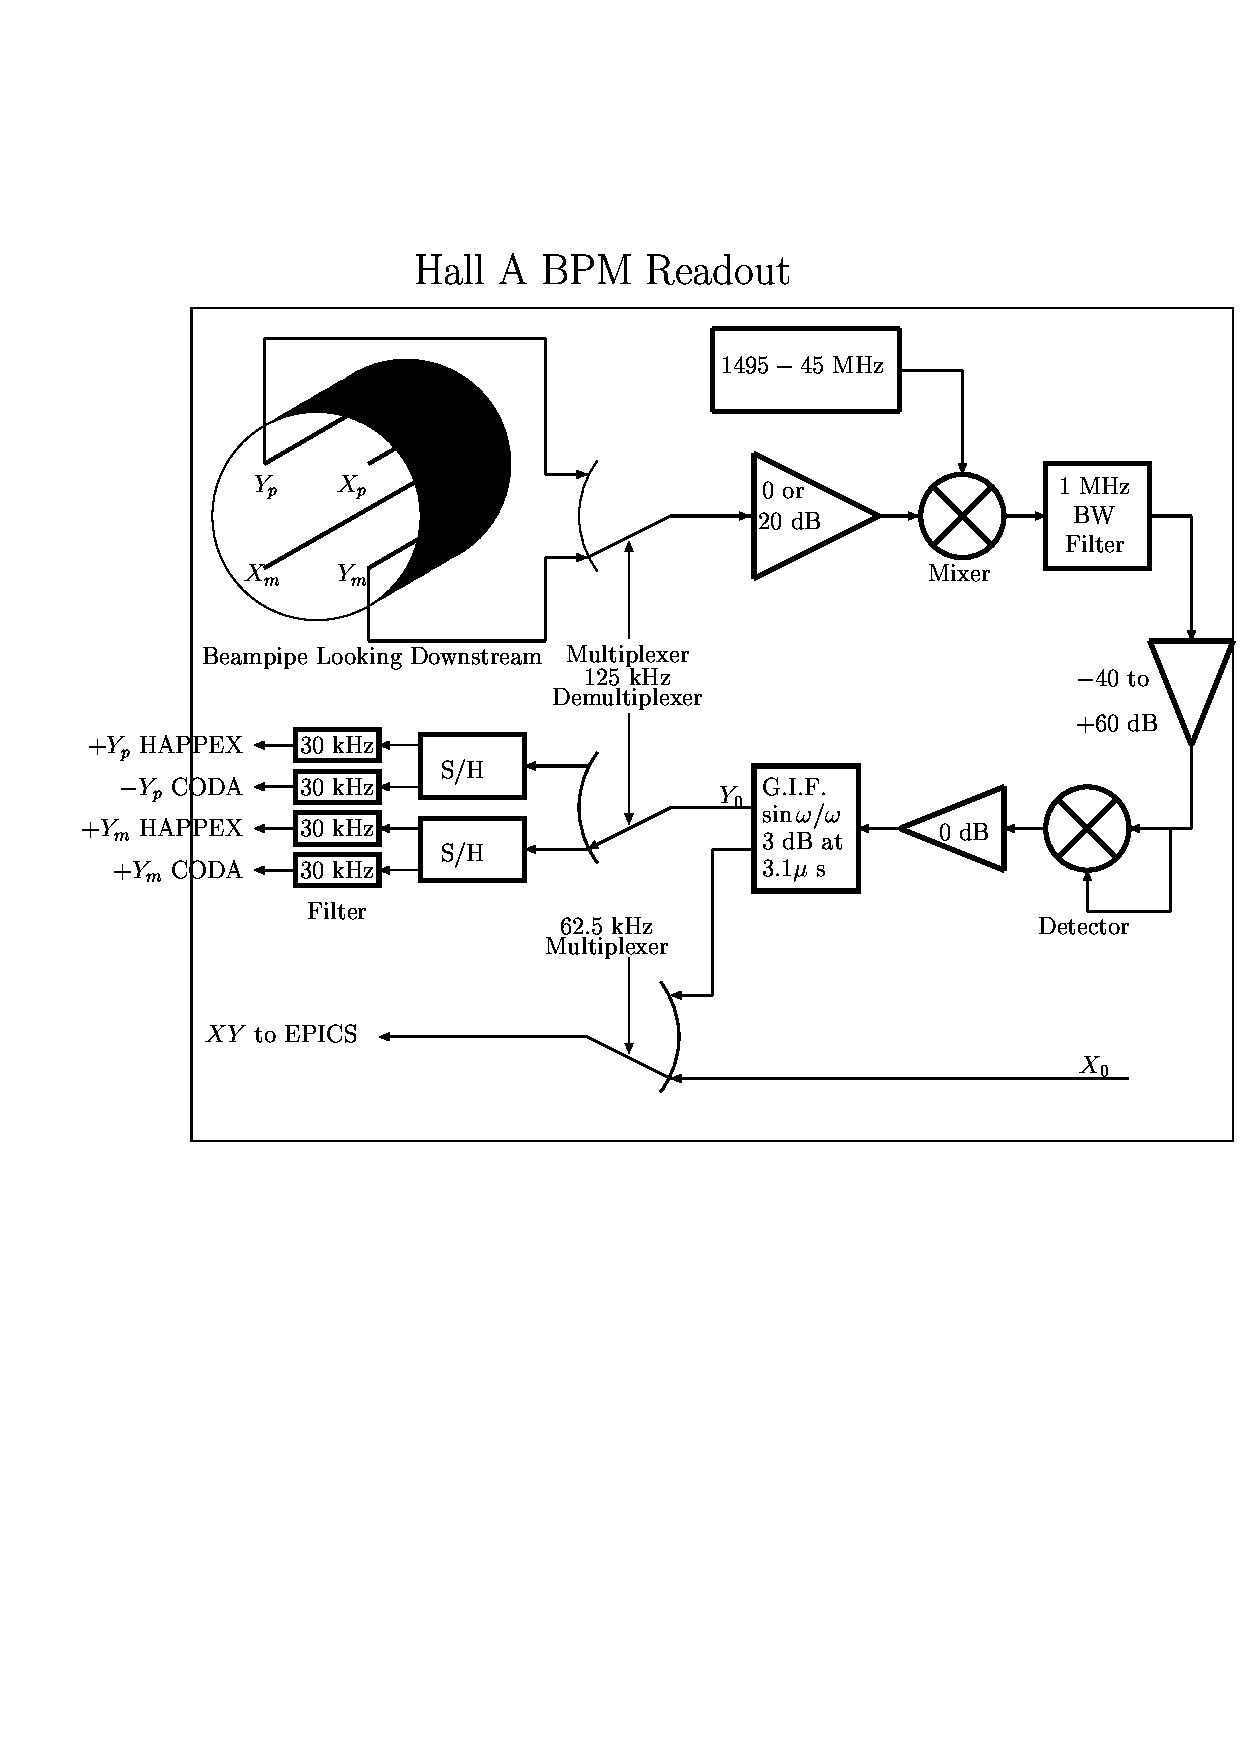
\includegraphics[angle=0,width=15cm]{BPM_fig}
{\linespread{1.}
\caption[Beamline: BPM Readout Electronics]{Schematic of the BPM readout
electronics}
\label{fig:bpmel}}
\end{center}
\end{figure}
}

1. The averaged position over 0.3 seconds is logged into the EPICS~\cite{EPICSwww} database (1 
Hz updating frequency) and injected into the datastream every 3-4 seconds, 
unsynchronized but with an orientative timestamp. From these values we can 
consider that we know the average position of the beam calculated in the EPICS 
coordinate system which is left handed.

2. Approximately once a shift (or more often if requested by the experimenters) 
a B-scope procedure ~\cite{bi:TP} can be performed using the same EPICS electronics 
which then gives the peak-to-peak variation of the beam.

3. Event-by-event information from the BPMs are recorded in the CODA datastream
from each of the 8 BPM antennas (2x4) from which the position of the beam can be 
reconstructed. However, these raw values belong to a parallel electronics chain 
whose constants have to be retrieved by calibrations to the EPICS or scanner 
data. 

\subsection{Beam Exit Channel}

After the target vacuum chamber, which was built by
the University of Virginia, there is an exit beam pipe which 
transfers the scattered beam onto the dump tunnel under vacuum. This exit beam 
pipe is made of a thin walled aluminum spiral corrugated pipe of welded 
construction. The largest diameter is 36 inches with a 0.164 inches wall 
thickness and the smallest diameter is 6 inches with a 0.042 inches wall 
thickness. The whole assembly is rather light (approximately 800 kg) and is 
supported by H shaped adjustable stands. To prevent possible linear collapse 
of the larger diameter sections under vacuum load, four aluminum channels of 
total cross-sectional area of 3'' are welded to its side. A vacuum of 
10$^{-5}$ Torr is maintained with a turbomolecular pump. The exit face of this 
pipe has a 12'' port and is connected to the diffuser with a Beryllium 
window.

}

\section{ Machine/Beamline protection system}
\label{sec:beam-fsd}

The MPS~\cite{MPScebaf} system is composed of the Fast Shutdown System (FSD), Beam Loss 
Monitor (BLM), and gun control system.

The FSD system is a network of permissive signals which terminate at the 
electron gun and chopper 1. The permissive to the gun and chopper
1 may be inhibited by any device connected to an FSD mode. Devices connected to the 
FSD system include vacuum valves, RF systems, Beam loss systems, beam current 
monitors, beam dumps, and particular to Hall A, the target motion mechanism 
and the raster (value and derivative).

The gun control system includes software program which monitors beam 
operating conditions and the state of the FSD and BLM systems. the program 
will warn the operators if a potential for beam damage exists. Potential for 
damage exists when running high average current beam, when FSD nodes are 
masked and when the beam power approaches the operating envelope limits for a 
specific beam dump.

\clearpage
\begin{safetyen}{10}{10}
\section{Safety Information}
\end{safetyen}
}
%
% Information for the ESAD
%

\begin{safetyen}{0}{0}

The beamline in the Hall provide the interface between the CEBAF accelerator
and the experimental hall.   All work on the beamline must be coordinated 
with both physics division and accelerator division; in order to ensure
safe and reliable transport of the electron beam to the dump.

\subsection{Hazards and Mitigations}

All magnets (dipoles, quadrupoles, sextupoles, beam correctors) and beam 
diagnostic devices (BPMs, scanners, Beam Loss Monitor, viewers) necessary for 
the transport of the beam are controlled by Machine Control Center (MCC) 
through EPICS~\cite{EPICSwww}, except for special elements which are addressed in the 
subsequent sections. The detailed safety operational procedures for the Hall 
A beamline should be essentially the same as the one for the CEBAF machine 
and beamline.\\ 

  
\noindent{}Personnel who need to work near or around the beamline should keep in mind the potential hazards:
\begin{itemize}
  \item Radiation ``Hot Spots'' - marked by ARM or RadCon personnel,
  \item Vacuum in the beam line tubes and other vessels,
  \item Thin windowed vacuum enclosers (e.g. the scattering chamber),
  \item Electric power hazards in vicinity of the magnets,
  \item Magnetic field hazards in vicinity of the magnets, and
  \item Conventional hazards (fall hazard, crane hazard etc.).
\end{itemize}

The most hazardous areas along the beamline are roped off it restrict access.   
In particule the scattering chamber, with it's large
volume and thin windows requires hearing protection once it has been evacuated.   
Signs are posted by radcon for any hot spots along the beamline and
radcon must be notified before work is done in a posted area.

Some magnets, as the M{\o}ller spectrometer elements, are covered with plastic
sheets for electric safety. Any access to these magnets requires
the ``Lock and Tag'' procedure~\cite{EHScebaf} and the appropriate training,
including the equipment-specific one. \\

\noindent{}Additional safety information is available in the following documents:
\begin{list}{--}{\setlength{\itemsep}{-0.15cm}}
  \item EH\&S Manual~\cite{EHScebaf};
  \item PSS Description Document~\cite{PSScebaf}
  \item Accelerator Operations Directive~\cite{AODcebaf};
\end{list}

\subsection{Responsible Personnel}

Since the beamline requires both accelerator and physics personnal to maintain
and operate and it is very important that both groups stay in contact that any 
work on the Hall A beamline is coordinated.

\begin{namestab}{tab:beam:personnel}{Beam line: authorized personnel}{%
   Beamline physics division and accelerator divison points-of-contact.}
  \namestabheader{Hall A Physicists}
  \DouglasHiginbotham{\em 1st Contact}
  \RobertMichaels{\em 2nd Contact}
  \namestabheader{Liaisons from Accelerator Division}
  \HariAreti{..to Physics}
  \YvesRoblin{..to Hall-A}
\end{namestab}
\end{safetyen}


\newpage
\section{ Beam Position Monitors}

To determine the position and the direction of the beam on the experimental 
target point, two Beam Position Monitors (BPMs) are located at distances 7.524 m 
(IPM1H03A) and 1.286 m (IPM1H03B) upstream of the target position. 
The BPMs consist of a 4-wire antenna array of open ended thin wire striplines 
tuned to the fundamental RF frequency of 1.497 GHz of the beam ~\cite{bi:bar90}. The 
standard difference-over-sum technique is then used ~\cite{bi:HW} to determine the 
relative position of the beam to within 100 microns for currents
above 1 $\mu $A. The absolute  position of the BPMs can be calibrated with respect to the 
scanners (superharps) which are located adjacent to each of the BPMs (IHA1H03A 
at 7.353 m and IHA1H03B at 1.122 m upstream of the target). The schematic of the 
readout electronics is shown in Figure ~\ref{fig:bpmel}. The
position information from the 
BPMs can be recorded in three different ways:

\begin{figure}
\begin{center}
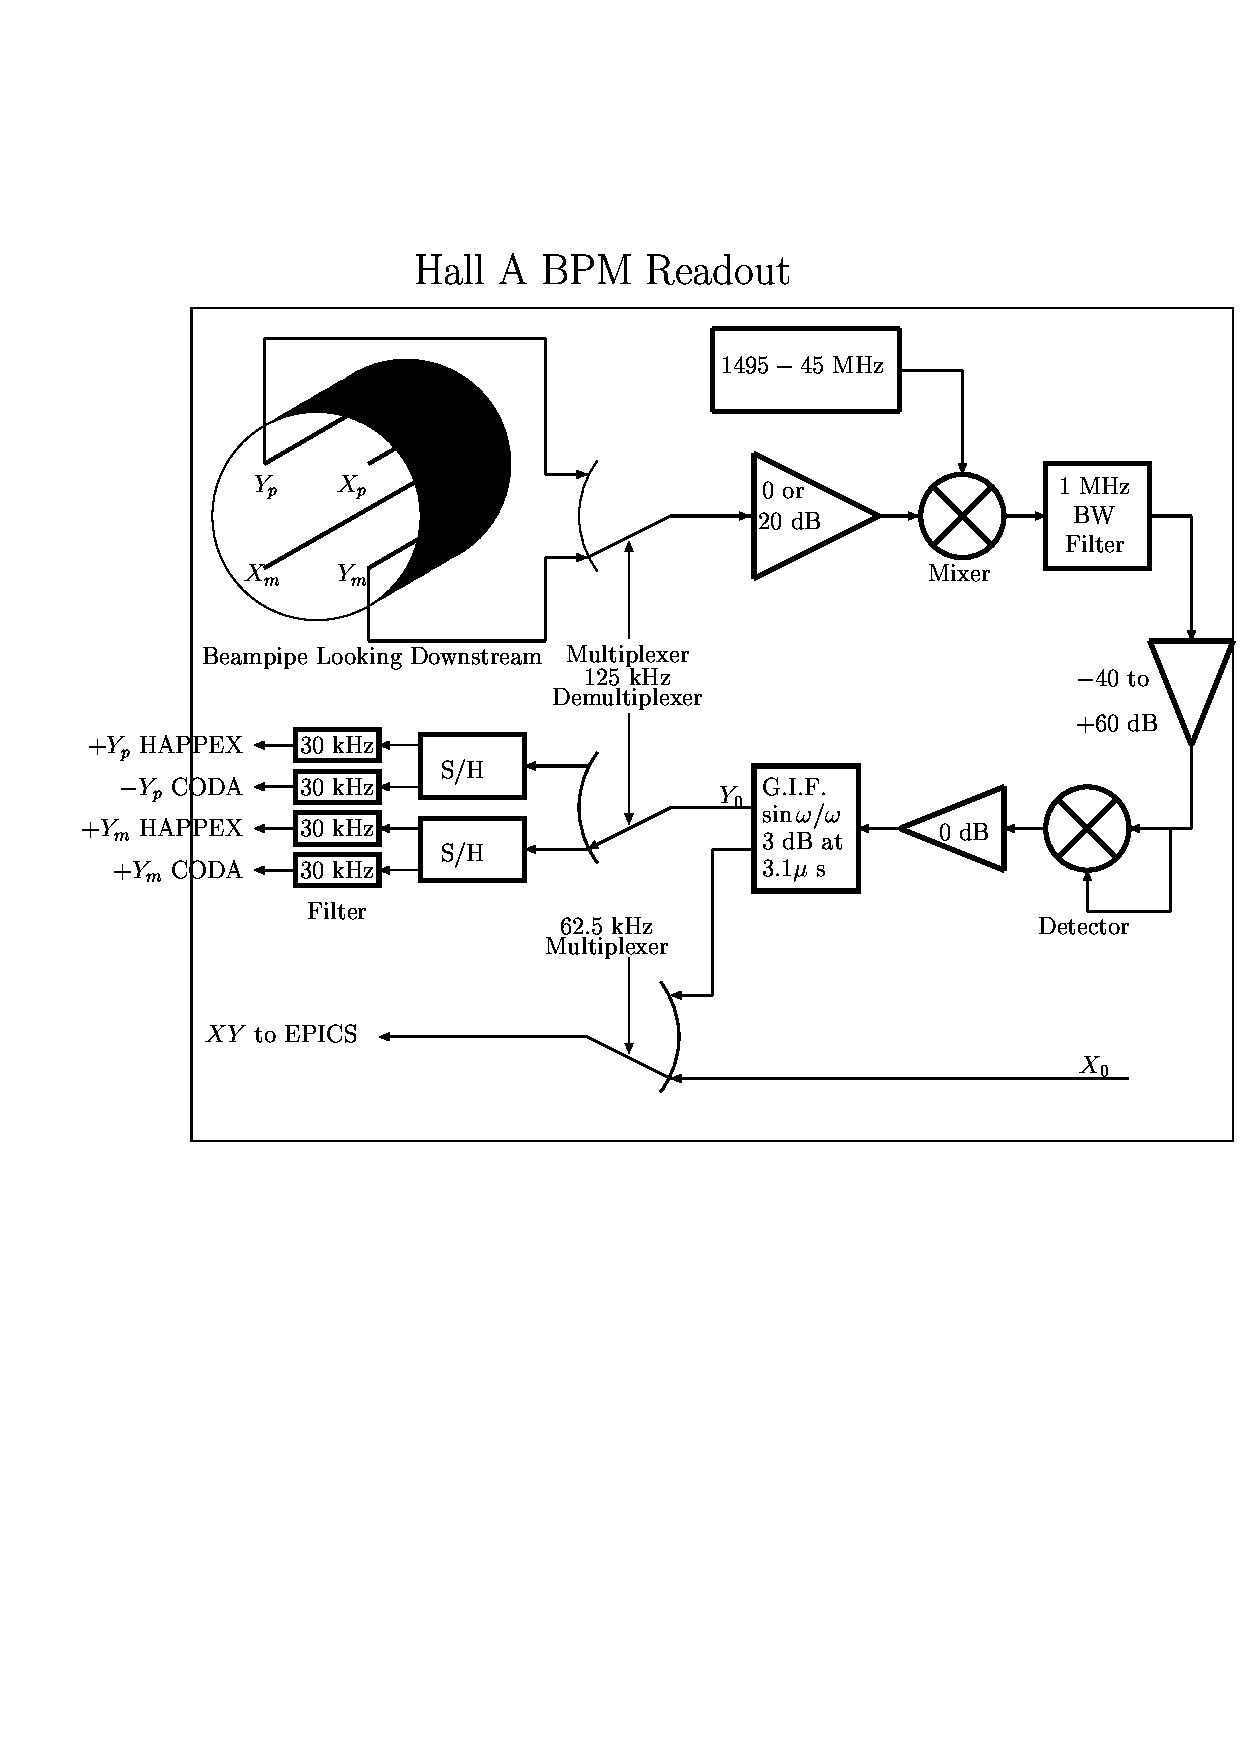
\includegraphics[angle=0,width=15cm]{BPM_fig}
{\linespread{1.}
\caption[Beamline: BPM Readout Electronics]{Schematic of the BPM readout
electronics}
\label{fig:bpmel}}
\end{center}
\end{figure}

\vskip 0.5cm

1. The averaged position over 0.3 seconds is logged into the EPICS database (1 
Hz updating frequency) and injected into the datastream every 3-4 seconds, 
unsynchronized but with an orientative timestamp. From these values we can 
consider that we know the average position of the beam calculated in the EPICS 
coordinate system which is left handed.

\vskip 0.5cm

2. Approximately once a shift (or more often if requested by the experimenters) 
a B-scope procedure ~\cite{bi:TP} can be performed using the same EPICS electronics 
which then gives the peak-to-peak variation of the beam.

\vskip 0.5cm

3. Event-by-event information from the BPMs are recorded in the CODA datastream
from each of the 8 BPM antennas (2x4) from which the position of the beam can be 
reconstructed. However, these raw values belong to a parallel electronics chain 
whose constants have to be retrieved by calibrations to the EPICS or scanner 
data. 


%\begin{thebibliography}{99}
%\bibitem{bi:bar90} W. Barry et al., CEBAF-PR-90-009 (1990).
%\bibitem{bi:HW} C. Hyde-Wright et al., Beam Position Studies for E93050 and priv. comm..
%\bibitem{bi:TP} T. Powers, priv.  comm.. 
%\end{thebibliography}
% ===========  CVS info
% $Header: /group/halla/analysis/cvs/tex/osp/src/beamline/bpms.tex,v 1.1 2003/06/05 17:28:32 gen Exp $
% $Id: bpms.tex,v 1.1 2003/06/05 17:28:32 gen Exp $
% $Author: gen $
% $Date: 2003/06/05 17:28:32 $
% $Name:  $
% $Locker:  $
% $Log: bpms.tex,v $
% Revision 1.1  2003/06/05 17:28:32  gen
% Initial revision
%

\newpage
\section[Beam Current Measurement]{Beam Current Measurement
\footnote{
  $CVS~revision~ $Id: bcm.tex,v 1.5 2003/12/13 06:23:37 gen Exp $ $
}
\footnote{Authors: A.Saha \email{saha@jlab.org}}
}

The Beam Current Monitor (BCM) is designed for stable, low noise, non-intercepting 
beam current measurements. It consists of an Unser monitor, two rf cavities, 
the electronics and a data acquisition system. The cavities and the Unser monitor 
are enclosed in a box to improve magnetic shielding and temperature stabilization.
The box is located 25 m upstream of the target. You can recognize it as a grey 
object on the stands, about 2 m downstream from where the beam enters the 
hall. 

The DC 200 down-converters and the Unser front end electronics are located in Hall 
A. The temperature controller, the Unser back end electronics and its calibration 
current source, cavity's RF unit (housing the RMS-to-DC converter board) and all 
multi-meters, VME crate and computers are located in Hall A control room.

\infolevone{
\subsection{ System Layout}

The schematic diagram of the BCM system is presented in
Fig.~\ref{fig:halla_bcm}.
\begin{figure}[htp]
\begin{center}
\includegraphics[angle=0,width=0.9\textwidth,clip]{habcm_r}
{\linespread{1.}
\caption[Beam Current Measurement: Schematic]{Schematic of the Hall A beam
current measurement system.}
\label{fig:halla_bcm}}
\end{center}
\end{figure}

The Unser monitor is a Parametric Current Transformer designed for non-destructive 
beam current measurement and providing an absolute reference. The monitor is 
calibrated by passing a known current through a wire inside the beam pipe and has a 
nominal output of 4 mV/$\mu $A. It requires extensive magnetic shielding and 
temperature stabilization to reduce noise and zero drift. As the Unser monitor's 
output signal drifts significantly on a time scale of several minutes, it cannot be 
used to continuously monitor the beam current. However, this drift is measured 
during the calibration runs (by taking a zero current reading) and removed in 
calibrating the cavities.  The more stable cavities are then used to determine the 
beam current and charge for each run. We also use the OLO2 Cavity Monitor and the 
Faraday Cup 2 at the Injector section to provide an absolute reference during 
calibration runs.

The two resonant rf cavity monitors on either side of the Unser Monitor are 
stainless steel cylindrical high Q ($\sim 3000$) waveguides which are tuned to the 
frequency of the beam (1.497 GHz) resulting in voltage levels at their   outputs 
which are proportional to the beam current. Each of the rf output signals from the 
two cavities are split into two parts. One part of the signal is  converted to 10 
kHz signals (by the ``downconverters'') and fed into an RMS-to-DC converter board 
consisting of a 50 kHz bandpass filter to  eliminate noise, amplified and split to 
two sets of outputs, which after further processing are recorded in the data 
stream. These two paths to the data stream (leading to the sampled and integrated
data ) will now be described. (The other part of the split signal is downconverted 
to 1 MHz signals and represents the old system (pre Jan 99). Only the HAPPEX 
collaboration presently uses these signals.)

For the sampled (or EPICS~\cite{EPICSwww} or Slow) data, one of the amplifier outputs is sent to a 
high precision digital AC voltmeter (HP 3458A). Each second this device provides 
a digital output which represents the  RMS average of the input signal during that 
second.  The resulting number is  proportional to the beam charge accumulated 
during the corresponding second (or, equivalently, the average  beam current  for 
that second). Signals from both cavity's multi-meters, as well as from the 
multi-meter connected to the Unser, are transported through GPIB ports to the HAC 
computer where they are recorded every 1 to 2 seconds via the data-logging process 
which is described in the calibration procedure. They are also sent through EPICS 
to CODA and the data stream where they are recorded at  quasi-regular intervals, 
typically every two to five  seconds.

For the integrated (or VTOF or Fast) data, the other amplifier output is sent to an 
RMS-to-DC converter which   produces  an analog DC  voltage  level. This level 
drives a Voltage-To-Frequency (VTOF) converter whose output frequency is  
proportional to the  input DC voltage level. These signals are then fed to Fastbus  
scalers and are finally injected into the data stream along  with the other scaler 
information.  These scalers simply accumulate during  the run, resulting  in a 
number which is proportional to the time integrated voltage level and therefore 
more accurately represents the true integral of the current and hence the total 
beam charge. The regular RMS to DC output is linear for currents
from about 5 $\mu$A to somewhere well above 200 $\mu$A.
 Since it is non-linear at the lower 
currents, we have introduced a set of amplifiers with differing gains (x3 and x10) 
allowing the non-linear region to be extended to lower currents at the expense of 
saturation at the very high currents. Hence there are 3 signals coming 
from each BCM (Upx1, Upx3, Upx10, Dnx1, Dnx3, Dnx10). All 6 signals are fed 
to scaler inputs of each spectrometer (E-arm and H-arm) . Hence we have a 
redundancy of 12 scaler outputs for determining the charge during a run. During 
calibration runs we calibrate each of these scaler outputs.   
}

\begin{safetyen}{10}{10}
\subsection{ Authorized Personnel}
\end{safetyen}

All Hall A members are authorized to take BCM calibration data using the Standard 
Non-Invasive Hall A BCM Calibration Procedure. The extended calibration procedures 
involving the Faraday Cup 2 and the OLO2 monitor at the Injector are presently 
performed by A. Saha. 

\vskip 0.2cm

The Accelerator AES group performs the maintenance of the BCM monitors. These 
include:

\begin{tabular}{l l}
1. The Unser calibration. & Every 3 months \\
2. Resonant Cavities Tuning. & Every Downtime \\
3. Multi-meters Autocalibration. & Every Downtime \\
4. Connectors Cleaning. &  Every year \\
5. Unser Keithley Current Source. & Calibration Yearly \\
6. Digital Multi-meters HP3458A and HP 34401A. & Calibration Yearly\\   
\end{tabular}

System Contacts are shown in Table~\ref{tab:BCM:personnel}.
\begin{namestab}{tab:BCM:personnel}{BCM: authorized personnel}{%
   Beam Current Monitor: authorized personnel}
  \ArunSaha{\em Contact}
  \JohnMusson{Accel. expert}
\end{namestab}
%Jean-Claude Denard -x 7555




% ===========  CVS info
% $Header: /group/halla/analysis/cvs/tex/osp/src/beamline/bcm.tex,v 1.5 2003/12/13 06:23:37 gen Exp $
% $Id: bcm.tex,v 1.5 2003/12/13 06:23:37 gen Exp $
% $Author: gen $
% $Date: 2003/12/13 06:23:37 $
% $Name:  $
% $Locker:  $
% $Log: bcm.tex,v $
% Revision 1.5  2003/12/13 06:23:37  gen
% Septum added. Name tables. Polishing
%
% Revision 1.4  2003/12/05 05:48:30  gen
% Polishing
%
% Revision 1.3  2003/06/06 15:19:02  gen
% Revision printout changed
%
% Revision 1.2  2003/06/05 23:29:59  gen
% Revision ID is printed in TeX
%
% Revision 1.1.1.1  2003/06/05 17:28:32  gen
% Imported from /home/gen/tex/OSP
%
%  Revision parameters to appear on the output

\newpage
\section[Fast Raster]{Fast Raster
\footnote{Authors: R.~Michaels \email{rom@jlab.org}}
}


The beam is rastered on target with an amplitude of
several millimeters at 25 kHz to prevent overheating.  
The raster is a set of four of air-core dipoles located
approximately 23 m upstream of the target. 
Two dipoles are for horizontal (X) motion and
another two for vertical (Y).  During the 6 GeV era
there was only one pair of X and Y, but we have doubled
the raster to account for the energy increase to 11 GeV.
The arrangement along the beamline along the 
direction of the beam will be XXYY.

For a typical 40A current in the raster coils, the
deflection by one pair (e.g. the X direction) of coils, 
in radians, is $\theta = 1.94 \times 10^{-3}/ E$
where $E$ is the electron's energy in GeV.
For example, at $E = 6$ GeV, a 0.32 mrad deflection is achieved.
Projected onto the target (about 21 m away) this is a $\pm$ 6.8 mm
excursion {\it if} there were no other magnetic fields 
between the raster and the target; however, there are quadrupoles
which change this depending on the beam tune.

Since 2003 we've used the triangle-wave 
raster pattern designed by Chen Yan.  
This achieves a very uniform rectangular
density distribution of beam on the target 
by moving the beam with a time-varying dipole
magnetic field whose waveform is triangular
with very little dwell time at the peaks.  
The electronics design is an ``H-bridge''
in which switches are opened and closed 
at 25 kHz, to switch between two directions 
of current (100 A peak-to-peak) 
through the raster coils.

Three new features during the 12-GeV era are 
1) the driver of the H-bridge electronics is now
an Agilent model 33522A waveform generator; and
2) The two X are synchronized with each other, and
the two Y are synchronized.  This makes the kicks
add and allows us to accomodate the higher energy
of the beam; and 3) The entire raster can
be synchronized to an external 10 MHz wavetrain
supplied by the polarized injector electronics.
This makes the nominal 25 kHz an exact multiple of
the helicity-flip rate, which achieves a cancellation
of raster noise, important for parity-violation 
experiments only.
The syncrhronization of the pairs of X and Y are
accurate to within a few nsec.

For most users, these three new features will not be
noticeable and the raster will appear to function
the same as during the 6 GeV running.
A user can view the 
status of the raster in the
EPICS overview screen called ``General Accelerator
Parameters'' where the set-point for the radius amplitude
and the readback of the peak-current in the raster are displayed.

Control of the raster is done by first asking the MCC
operators to set up the raster for a particular size
typically 2 mm square.
The control software assumes a field-free region between
the raster and the target, so it is only approximately
correct because there are several quadrupoles in this region.
It is important to check the raster spot size and
make adjustments if necessary.  The adjustment is made
by asking MCC to change the size and noting the 
linear relationship between what their software says
the size is and the actual size.
Relatively small independent adjustments to the 
gains on the X and the Y raster
coils are available in the middle room of the hall A
counting room using the ``PGA Controller'' knobs;
however, it is not recommended to touch these.
Near these knobs is also located an oscilloscope X-Y trace
of the current in the raster.  A fast shutdown (FSD) shuts
the beam down within 0.1 msec if the raster fails, thus
affording some protection of the target.

{\it NOTE:  If you are unsure of the status of the raster,
measure the spot size with very low current ($\le 2 \mu$A) or with
the target out of the beam.}  It would be a mistake
to check the beam spot size with high current on target; by
the time you check it, the target may already be destroyed.
The rastered beam spot on target can be checked with
plots in the ROOT analyzer or by 
using the stand alone code called \mycomp{spot},
also called \mycomp{raster}.
For more details on usage, type \mycomp{spot -h} (help)
on the ADAQ computers.

Regarding the BPM measurements, it should be noted that 
the stripline BPMs displayed by \mycomp{spot} have a high-frequency 
cutoff of approximately 30 kHz.  Since the raster frequency is 25 kHz
the plot of the amplitude distribution shows spikes at the 
limits of the orbit, instead of a flat distribution.  The scale
factor between what is seen in \mycomp{spot} and the real width of the beam
is $\sim 1.5$, i.e. the beam is 1.5 times bigger than the naive
reading of the \mycomp{spot} distribution.



\newpage
% Updated Comments Dec. 2
\infolevone{
\chapter[Arc Energy Measurement]{Arc Energy Measurement
\footnote{Authors: D. Higinbotham \email{doug@jlab.org}}
}
}

\infoleveqnull{
\section{Arc Energy Measurement}
\subsection{Overview}
In order to determine the integral field of the eight dipoles that lead to Hall A, and 
in turn determine the beam energy, a nineth dipole wired in series with the rest is 
located in a special shed near the hall A counting house.
}

\infolevone{
The ARC energy measurement is under EPICS~\cite{EPICSwww} control through 
a MEDM~\cite{MEDMwww} display. Two
independent control systems are used: the beam bend angle measurement through
the arc ("scanners") and the field integral of
the arc ("integral"). To measure the energy: 

\begin{itemize}
\item perform several angle measurements 
\item perform an integral measurement 
\item analyze the integral measurement and note the value of the arc field 
integral 
\item analyze the angle measurements, average the results (proposed by the 
software),
then ask for the energy calculation, enter the above arc field integral and
you will get the beam energy computed from the average angle. 
\end{itemize}

\section{Summary of ARC operations }

Six scanners of the same type, called ``ARC scanner'' and labelled
from scanner \#1 to \#6, are installed on the Hall-A beamline. Scanners \#1
to \#4 are used for the ARC energy measurement and they are located on the Hall-A
arc: \#1 [1HA1C07A] and \#2 [1HA1C07B] just upstream of the arc, in the BSY, and 
\#3 
[1HA1C18A] and \#4 [1HA1C18B] in the Hall-A
tunnel, just upstream the Compton polarimeter. Scanners \#5 [1HA1H03A] and \#6 
[1HA1H03B] 
are located
between the Moller and the target to control the beam geometry on the target
and their use will not be discussed here. 

Procedure for running a harp scan is described elsewhere\footnote{
Harp scan procedure \url{http://hallaweb.jlab.org/equipment/beam/harp_halla/harp.html}.}

Each scanner has a motor/ball-screw/shaft-encoder/vacuum-penetrator system moving
accurately a set of 3 tungsten wires through the beam. Each time a wire crosses
the beam a PMT located a few meters downstream records a signal due to the 
electromagnetic
shower induced by the beam in the wire. Both forward and backward passes are
recorded. The motion is a horizontal translation and, for a forward pass: 

-the translation is from beam left to beam right, 

-the two first wire crossing the beam are at 45deg from the vertical, 

-the third wire, which is the only important for the ARC energy measurement,
is vertical. 

Recording, during the scan, the scanner position and the PMT output voltage
allows us to determine the beam position at each scanner location. Then, using
calibration data not detailed here, we deduce the net beam bend angle through
the arc. This result measured in dispersive arc tuning, along with the field
integral of the arc dipoles, provides an accurate determination of the beam
energy. 

\vspace{0.3cm}

\section{Summary of field integral }

The purpose is to measure absolutely the straight field integral of a 
"BA"
3m long dipole, called the "9th dipole" and located in the
"Dipole Shed". It is of the same type as the 8 arc dipoles
and is powered in series with them. 

The ARC integral setup is basically made of a 3m long plate (the 
"probe")
which is able to move inside the 9th dipole gap along the beam axis and carrying 
two
field measurement devices: a pair of pick-up coils connected in series and a
set of NMR probes. The coils are on both ends of the probe and the NMRs close
to the center. 

-at the "upstream" probe position, the 
"downstream"
coil is close to the dipole center, the "upstream" is outside
the dipole and the NMRs at one end of the dipole: 

Door$<-$-- ....................$<-$-------DIPOLE-----$--->$ 

.............$<-$-------PROBE------$--->$ 

-at the "central" probe position, each coil is at one end
of the 3m long dipole and the NMRs close to the dipole center: 

Door$<-$-- ...................$<-$-------DIPOLE-----$--->$ 

..................................$<-$-------PROBE------$--->$ 

-at the "downstream" probe position, the 
"upstream"
coil is close to the dipole center, the "downstream" is outside
the dipole and the NMRs at one end of the dipole: 

Door$<-$-- ...................$<-$-------DIPOLE-----$--->$ 

....................................................$<-$-------PROBE------$--->$ 

We call upstream the position where the probe is the closest to the shed access
door. Among the 3 above positions, the only one where the NMR can lock on the 
dipole
field is the central one as in the extreme position of the probe, the field 
homogeneity
is not sufficient. The probe position is controlled by a linear encoder. The
Z axis refers to the "beam" direction, increasing from upstream
to downstream. We use three kinds of "Z": 

-Zm to locate a point inside the magnet. The dipole center is at Zm=0 and the
yoke ends at +-1500.mm 

-Zp to locate a point inside the probe. The probe center is at Zp=0. Each of
the 4 NMR probes has a Zp given in the file "magnet.dir".
At a temperature of 21C, the coils are at Zp=+-1519.815mm (from magnet.dir) 

-Zd to refer to a displacement of the probe w.r.t. the dipole. Zd=0 refers to
the upstream (home) position of the probe. The integral measurement is performed
from Zd=0.000mm (1st PDI trigger) to Zd=3199.000mm (last PDI trigger), for forward
pass. Zd is given by the display (at the top of the rack) or by the master screen
("OUT"). 

The relationship between Zm, Zp and Zd is: 

Zd-Zm+Zp=C 

where C is a constant given in magnet.dir (C=1604.000 nomin.). Example of use:
to have the probe center at the dipole center, one must set Zd=1604.000mm (set
Zm=0 and Zp=0 in the above formula, and solve for Zd) 

The integral measurement sequence is the following: 

-from the current position (a priori arbitrary) move the probe upstream, up
to a limit (optic) switch. 

-move downstream by a few mm to cross the encoder index (encoder initialization) 

-move to the central position to measure the central field by NMR, the system
checks if the NMR locks and if the reading is stable, it will be the 
"before"
field 

-move back to upstream position 

-move to downstream position while integrating the flux through the coil system,
this measurement will be called the "forward" integral (duration
\( \sim  \) 7s) 

-move back to upstream position while integrating the flux through the coil
system, this measurement will be called the "backward" integral
(duration \( \sim  \)7s) 

-move to the central position to measure the central field by NMR, the system
checks if the NMR locks and if the reading is stable, it will be the 
"after"
field. 

In addition to the central field, 4 probe temperatures, a local excitation current
measurement, the setting of the dipoles P.S, the readback of the dipoles P.S
and the probe position at NMR measurement time are recorded 
"before"
and "after". 

To perform an integral field measurement: 

1-check if the system works (see "details on integral system 
check"
below) 

2-run the above integral sequence (see "details on integral run"
below) 

3-fix the error(s) if any (see "details on integral errors"
below) 

4-save the data in a file (see "details on integral data save"
below) 

5-analyze the data  


\section{Details on integral run }

To run the integral measurement sequence, call the 
\mycomp{arc\_integral.adl}
medm screen, then: 

-push "start" to start the full sequence 

-look at the results displayed: 

-after the "before" NMR measurement: the 
"before"
data set 

-after the "forward" integral pass: the forward velocity profile
and the forward voltage-after-gain profile 

-after the "backward" integral pass: the backward velocity
profile and the backward voltage-after-gain profile 

-after the "after" NMR measurement: the 
"after"
data set 

-if "BAD NMR" or "PDI saturation" flags
are set, or if something is obviously wrong in the data or plots, call expert. 

-data are ready to be saved (see "Details on integral data save"
below) 


\section{Details on temperatures }

The AC system of the shed is made of two cooling units, a heating unit and a
controller connected to two temperature sensors : one located in the shed and
one located in the BSY. This system is programmed in such a way that the 
temperature
of the shed follows the BSY temperature within +-2C. The BSY temperature can
be anywhere in the 18C to 35C range, regardless of the season. The BSY 
temperature
and the shed temperature are given (in F) by a display panel located close to
the workstation, on the wall. The AC system can be set in manual control by
turning from "auto" to "manual" a set of
switches controlling the cooling units and the heater unit. These switch boxes
are located on the shed wall. If the shed temperature is above 34.4C (94F),
call the crew chief (the electronics can be damaged) and cool down the shed in manual
AC mode. The 4 temperature sensors of the probe are labelled Tx+z+, Tx+z-, Tx-z+,
Tx-z- depending on their position w.r.t. the frame. 

Both "x+" sensors are on the probe edge which is inside the
dipole gap and both "x-" sensors on the opposite edge which
is outside the dipole gap. Both "z-" sensors are at 1/4 of
the long dimension of the probe and both z+ at 3/4 of this length. The average
of the 4 temperatures is used by the analysis program to correct the coil distance
from the thermal expansion of the probe, so it is important to make sure that
the 4 sensors are working well. The user can just make sure that the temperatures
displayed in \mycomp{arc-master.adl} or recorded in 
\mycomp{arc-integral.adl}
are realistic. In \mycomp{arc-integral.adl} they are given in the
order: Tx+z-, Tx+z+, Tx-z-, Tx-z+ Tx-z- and Tx-z+ should be close to the shed
temperature. Tx+z- and Tx+z+ depend on the probe position, as the gap (iron
yoke) is warmer than the shed and the dipole coil (at both ends of the dipole)
is warmer than the iron yoke. For a probe in a central position for more than
about one hour, the Tx+z- and Tx+z+ sensors should give the yoke temperature,
i.e the shed temperature plus 0. to 5.C, depending on the current, LCW temperature
and the magnet/shed temperature history. The 4 temperatures are also displayed
inside the shed, on the electronics rack. These values are digitized by separate
ADCs, so they may differ from the remote values by \( \sim  \)0.1C. 
}

\begin{safetyen}{10}{10}
\infolevone{\section{Shed access and safety }}

Due to the the dipole magnet and motion system, the access to the shed is limited to authorized
persons which are listed in the ESAD and listed below. To be added to the list, 
contact Douglas Higinbotham.
The standard
operation mode of the integral measurement setup is the remote mode, through
the network, from the counting house.
\end{safetyen}

\begin{safetyen}{10}{10}
\infolevone{\section{List of Authorized Personnel for Shed Access}}
\infoleveqnull{\subsection{List of Authorized Personnel for Shed Access}}
\end{safetyen}
\begin{namestab}{tab:arc:personnel}{Arc Energy Measurement: authorized personnel}{%
                 Arc Energy Measurement: authorized personnel}
  \namestabheader{Hall A Personnel}
  \DouglasHiginbotham{\em Contact}
  \namestabheader{Accelerator Personnel}
  \MichaelTiefenback{}
  \YvesRoblin{}
  \RickGonzales{}
  \BillMerz{}
  \MarkAugustine{}
  \HariAreti{}
  \PeteFrancis{}
  \ScottHiggins{}
  \DavidSeidman{}
  \RonLauze{}
  \TonyDay{}
  \ChristopherCurtis{Alignment group}
  \namestabheader{CEA - Saclay experts}
  \PascalVernin{}
  \ChristianVeyssiere{}
  \FrancoisGougnaud{}
  \JacquesMarroncle{}
\end{namestab}



\newpage
\infolevone{
\chapter[Target Chamber]{Target Chamber
\label{sec:target_chamb}
\footnote{
  $CVS~revision~ $Id: tgtcham.tex,v 1.11 2005/04/04 22:27:25 gen Exp $ $
}
\footnote{Authors: ?? \email{??@jlab.org}}
}

The cryo-targets and the waterfall targets 
(see Sec.~\ref{sec:targets-overv}) 
are contained in a special target chamber which is a large 
evacuated  multistaged can. So far, three chambers have been designed:
\begin{list}{\arabic{enumi}.~}{\usecounter{enumi}\setlength{\itemsep}{-0.15cm}}
  \item a chamber used up to 2003;
  \item a chamber designed for use with septum magnets, starting in 2003;
  \item a chamber designed for use with the BigBite spectrometer.
%\footnote{
%        No yet manufactured by Dec,2003.}.
\end{list}

Here, chamber 1 is described. Chambers 2 and 3 are only different in 
size and slightly in shape. The safety considerations fully apply to chambers 2 and 3.
The chamber was designed to isolate the beam line vacuum from  each
HRS so that each HRS could rotate
around the target without vacuum coupling and without jeopardizing
certain desired kinematic and acceptance  specifications of 
both high resolution spectrometers
needed for approved experiments.  It  was also designed to simultaneously
 contain a liquid or gas target and an array of water cooled thin
 metallic foils, both remotely controlled and also be adaptable for
the waterfall target. The desired kinematic specifications that were
 considered included momentum and energy resolution in both arms,
 angular range of spectrometers, angular acceptance, and luminosity.
The chamber vacuum is isolated from the  HRS by using thin aluminum foils. 

The target chamber is designed so that
each spectrometer will have continuous coverage in the standard tune from
$\theta_{min}=$12.54$^\circ$ to $\theta_{max}=$165$^\circ$.
The aluminum window is 6~$in$ high and 0.016~$in$ thick made of 5052 H34 aluminum foil.
The foil forms regularly spaced vertical ridges when
placed under load. The window had an inter-ridge
spacing of 3 inches.
If the window is treated as a collection
of smaller rectangular windows which have the full vertical height
of 6 inches and the inter-ridge spacing as a width,
then stress formulas predict that the 0.016 $in$
material would reach ultimate stress at a pressure higher than 35 PSID
(for both over-pressure and under-pressure). 
There is a gate valve between the 
scattering chamber and the beam entrance (exit) 
pipe. Both 
valves will be closed automatically in the
event that the chamber vacuum begins to rise and an FSD will be caused
( this is done via a relay output of the scattering
chamber vacuum gauge). If either valve is closed an FSD will result.

The target chamber is supported by a 24 $in$ diameter pivot post
secured in concrete, rising about 93.6 $in$ above the Hall A cement floor.
The Hall A target chamber
consists of an aluminum middle ring, a stainless steel base ring,
each with a 41.0 $in$ inner diameter,
and a stainless steel cylindrical top hat with 40 $in$ inner diameter
to enclose the cryotarget and secure the cryogenic connections.

When the scattering chamber is under vacuum, there is a potential
danger of window rupture.
The loud noise from the rupture could hurt
one's ears if not protected. Therefore when the chamber is under vacuum,
protective covers are put on if possible. These must be taken off
for data taking. For restricted access, the protective cover is required
to be on when the chamber is under vacuum. Before switching from controlled
access to restricted access, the protective cover is required to be installed.
Anytime that the scattering chamber
is under vacuum, the pivot area is enclosed in a rope or tape barrier
and a warning sign is posted.
Hearing protection is required in the enclosed area.

\infolevone{
	The aluminum ring with an outer diameter of 45.0 $in$ and
wall thickness 2.0 $in$  is necessary for a sturdy support structure and
to permit machining of the outside surface to accommodate
the flanges for fixed and sliding seals mounted on
opposite sides of the ring that vacuum connect the chamber to each HRS.
The height of the aluminum ring shown is 36.0 $in$, which is
designed to accommodate the mounting flanges.
The stainless steel base ring 
is 11.50 $in$ in height with
one pump-out 6 $in$ diameter port  and with
seven 4 $in$ viewing and electrical feed-through ports.
The base ring will also contain support mechanisms for the solid
target ladder assembly, a rotisserie for collimating slits, radiators, and
magnetic
fingers for
removing the solid target vacuum-lock can. The total height of the top
ring, middle ring, and
base ring is 93.81 $in$. This length is partly determined by our desire to
include with the cryogenic extended target a solid target vertical ladder
secured in an inverted hat through a hole in the base of the chamber.

	The base ring includes an end plate through which the
inverted hat will be adapted to fit into the large vertical pipe serving
as the pivot post for the Hall A spectrometers.

	The stainless steel cylindrical top hat  has
40.0 $in$ inner diameter, and is 0.375 $in$ thick and
46.31 $in$ high , which is necessary to permit the
cryotarget to be withdrawn and to make space available to expose the solid
targets to the electron beam.

   The 200 $\mu$A electron beam, focused to a $\sim$\(0.1\, mm\times
0.1\) mm spot and rastered $\pm$5 mm horizontally or vertically on the
target, enters through a oval hole in the middle ring which
is 2.06 $in$ wide and exits through a 1.81 $in$ hole connected to the
exit pipe.
}

\infolevone{
\section{Target Chamber - Spectrometer Coupling}

   The aluminum middle ring will support a flange on each side for each high
resolution spectrometer. Four flanges will be available: Two flanges will
contain a 6 $in$ window opening which will be covered with a thin foil
(e.g., 10 mil aluminum) .
These two flanges will be used for experiments utilizing
extended  targets that do not require optimum momentum resolution.
The other two flanges will have two fixed ports (with a 8 $in$ $\times$ 6 $in$
opening)
which will be mainly used for calibration of the spectrometers . Fixed ports are
centered at 16.11 $^\circ$ and
45 $^\circ$ for one flange and at 16.11 $^\circ$ and 90 $^\circ$ for the second
flange.

   For a point beam on target a vertical opening in the walls of the chamber
of height 57.15 cm x 0.065 x 2 = 7.43 cm is required so that the scattered
beam is within the full acceptance of the spectrometer.
If the beam is rastered on target $\pm$0.5 cm in the vertical direction,
then the opening in the outer side of the chamber must be at least 8.5 cm for
full acceptance.

From consideration of the angular range of the spectrometers in the standard
tune, the scattered beam acceptance envelope, the effects of an
extended gas target on acceptance,
and the effects of a rastered beam $\pm$ 5 mm on acceptance,
the target chamber requires a window of at least 8.5 cm
high in the aluminum ring extending from 6.33 $^\circ$ (2.48 in) from the
beam exit point to 8.83 $^\circ$ (3.47 in) from the beam entrance point on one
side and a similar window on the other side of the beam.
For future considerations (e.g., using a third arm or sliding seal) the
width of the window on the middle ring was actually constructed
to be 17.78 cm (7 $in$).

\section{Stress Analysis of the Middle Ring}

Since the middle ring has an extensive cut across the midplane on both sides as
well as
entrance and exit holes and loaded with about 25,000 lbs, calculations of the
stresses
 and deformation of  the
midplane support area of the middle ring and deflection of the window opening
were made using the finite element analysis code ANSYS . The work was conducted
by a graduate student in the Department of Civil Engineering at the
University of
Virginia and a REU student.  A scaled down model of the middle ring was
constructed and then tested by applying forces to it using the Materials Testing
Service of the Department of Transportation at the University. ANSYS was first
checked by comparing calculations of the test model deflections to the actual
data. Agreement was  within $\pm$10\%. Results of ANSYS for the target
chamber showed that the maximum deflection of the opening of the window in the
middle ring varied from 0.007 $in$ to 0.015 $in$ depending on how the
middle ring
was loaded. This was decided to be a safe limit. In the final design, several
movable
7 $in$ long, 2 $in$ diameter aluminum support rods are placed in the
window for added support. In addition, flanges defining the ports and
coupling to
the spectrometers can be added, giving additional support to the middle ring.
Compressional stresses, calculated using ANSYS assuming the middle ring was
attached to the
top hat and loaded with 25,000 lbs, were less than 3000 psi 
almost everywhere.
However, stresses over small areas rose to levels 6000 psi near the entrance
and exit holes. These calculations indicated that we did not exceed the safety
limit of 15,000 psi for aluminum. A simple model calculation shown in Appendix
A  gives the result 1434 psi, which represents some average value over the
midplane
contact area.

\section{Vacuum Pumping System}

The vacuum in the target chamber is maintained by an Alcatel ( 880 l/s)
 turbomolecular vacuum pump. The pump is connected to a 6 $in$ port in the
stainless steel ring between 130
 $^\circ \le \theta_p \le 180 ^\circ$. The vacuum pump is
fastened to a horizontal pipe connected to the chamber. The vacuum pressure in
the chamber is about $10^{-5}$ mm. An additional Alcatel pump connected
to an 8 $in$ port should be added to obtain lower vacuum. Both
pumps may be isolated
from the target chamber using gate valves which are remotely operated
from the vacuum control rack and interlocked to the FSD system.


A 2 $in$ all metal gate valve is located between the entrance flange to the
chamber and the beam profile monitor.   
 An additional gate valve is located 2 m downstream of the
 target chamber to isolate the chamber from the exit beam pipe.
}
\begin{safetyen}{10}{15}
\section{Safety Assessment}
\end{safetyen}

The scattering chamber is typically a low maintenance item but it is a vacuum
system and hence problems may occur. The day to day operations of the cryogenic
targets are managed by the Hall A Staff while major maintenance operations are
handled by the Cryogenic Target Group (Physics Division). Occasionally the
cryogenic targets experience difficulties due to failures of the End Station
Refrigerator which supplies the coolant. In these cases the Cryogenics Group
of the Accelerator Division should be contacted.

\noindent{}The target chamber may pose several hazards:

\begin{list}{\arabic{enumi}.~}{\usecounter{enumi}\setlength{\itemsep}{-0.15cm}}
  \item {\bf Rupture of vacuum windows}. This hazard is mitigated by
        lexan guards on the vacuum windows, installed by the hall technicians
        either at the beginning of a ``restricted access'' period 
        %(see Sec.\ref{sec:Access}),
        or during ``control access'', in case an access to the target chamber area is needed.
        Installation and removal of the guards is included in the technician's checklists.
        When the chamber is under vacuum, it is mandatory to use ear protection in the chamber
        vicinity. The appropriate signs must be installed by the technicians. 

  \item {\bf Induced radioactivity}. The RADCON surveyor measures the level of induced
        radiation as a part of the general survey and may declare the target area 
        as ``High Radiation Area'', installing a rope protection around\cite{RWIcebaf}. 

\end{list}

Some other safety issues are discussed in the cryo-target chapter 
(see Sec.~\ref{sec:target-cryo-safety}).
%and also in the polarized target chapter (see Sec.~\ref{sec:target-he3-general}).

\begin{safetyen}{10}{15}
\section[Authorized  Personnel]{Authorized  Personnel}
\end{safetyen}

\begin{namestab}{tab:targ_chamb:personnel}{Target chamber: authorized personnel}{%
      Target chamber: authorized personnel. ``W.B.'' stands for the white board 
      in the counting house.}
  \TechonCall{\em Contact}
  \JessieButler{}
  \DaveMeekins{Target group}
  \JianPingChen{}
\end{namestab}
}

\newpage
\infolevone{\chapter[M{\o}ller Polarimeter]{M{\o}ller Polarimeter}
\setcounter{subsection}{0}}
\infoleveqnull{\section[M{\o}ller Polarimeter]{M{\o}ller Polarimeter}}

The Hall A beam line is equipped with a M{\o}ller 
polarimeter
whose purpose is 
to measure the polarization of the electron beam delivered to the hall. 

\begin{safetyen}{0}{0}

The M{\o}ller Polarimeter system has under gone a major upgrade and an Operational Safety Proceedure (OSP)
is being written and must be reviewed before its use.

\subsection{Hazards and Mitigations}

The hazards and mitigations for this system can be found in the OSP at the end of this document. 

%\infolevone{
%Safety checklist item for this device, located at the end of the beamline section, is solely to ensure
%the beam can be tranported safetly past this system prior to it's recommisioning.
%}

\subsection{Responsible Personnel}
\label{sec:moller-pers}

This list of system experts provided in case there is any question as to the status of system.

\begin{table}[h]
\begin{center}
\begin{tabular}{|ll|l|l|l|l|r|} \hline
  \multicolumn{2}{|c|}{Name} & Dept. & \multicolumn{2}{c|}{Telephone} & 
  \multicolumn{1}{c|}{e-mail} & Comment \\ 
  \cline{4-5}
   &  &   & JLab & Pager &  & \\ 
\hline
 Javier       & Gomez           & JLab    & 7498 & 7498 & gomez@jlab.org    & Primary contact     \\ 
 Oleksandr    & Glamazdin       & Kharkov & 5441 & 5441 & glamazdi@jlab.org &  \\ 
 Viktor       & Gorbenko        & Kharkov & 5441 &   -  & gorbenko@jlab.org &  \\ 
 Roman        & Pomatsalyuk     & Kharkov & 5395 & 0001 & romanip@jlab.org  &  \\ 
\hline
\end{tabular}
\end{center}
\caption[Moller Polarimeter: authorized personnel]{
   The listed name are those who are considered system experts of the Moller Polarimeter and should be contacted
   if there is any question as to the status of the system.
}
\label{tab:moller:personnel}
\end{table}
\end{safetyen}


\newpage
}
% Compton Polarimeter
\infolevone{\chapter[Compton Polarimeter]{Compton Polarimeter}
\label{sec:compton}
\footnote{Author: S.Nanda \email{nanda@jlab.org}}
}
\infoleveqnull{\section{Compton Polarimeter}
\subsection{Overview}}


The Hall A Compton polarimeter has undergone a major upgrade and an
new operational safety proceedure (OSP) is being written and reviewed before the
Compton can be used.   The hazards and mitigations for this system can be found in 
this OSP.

\subsection{Responsible Personnel}

\begin{namestab}{tab:compton:personnel}{Compton Polarimeter: authorized personnel}{%
          Compton Polarimeter: authorized personnel}
 \SirishNanda{Primary Contact}
 \JackSegal{Secondary Contact}
\end{namestab}

\infolevone{
\subsection{Authorized Personnel}

The list
of the presently authorized personnel is given in Table~\ref{tab:compton:personnel}.
Other individuals must notify and receive permission from
the contact person (see Table~\ref{tab:compton:personnel}) to get their names
add to list.

\begin{namestab}{tab:compton:personnel}{Compton Polarimeter: authorized personnel}{%
          Compton Polarimeter: authorized personnel}
 \SirishNanda{\it Contact}
 \JackSegal{Technical}
 \JosephZhang{Optics}
 \MartialAuthier{Engineering}
 \NathalieColombel{Mechanical}
 \PascaleDeck{Electronics}
 \AlainDelbart{Optics}
 \DavidLhuillier{Analysis}
 \YvesLussignol{EPICS}
 \DamienNeyret{DAQ}
 \GerardTarte{Electronics}
 \ChristianVeyssiere{Electronics}
\end{namestab}
}



%
% Old Material
%
% \chapter[eP Beam Energy Measurement]{eP Beam Energy Measurement
\footnote{
  $CVS~revision~ $Id: ep.tex,v 1.6 2003/12/13 06:23:37 gen Exp $ $
}
\footnote{Authors: B.Reitz \email{reitz@jlab.org}}
}
\label{sec:ep}
\section {Purpose and Layout}
\label{sec:ep_purpose}

The Hall A eP system is a stand-alone device to measure the 
energy of the electron beam. It is located along the beamline
17~m upstream of the target. The beam energy $E$ is determined by measuring
the scattered electron angle $\Theta_e$ and the recoil proton angle
$\Theta_p$ in the $^1$H$(e,e'p)$ elastic reaction according to the kinematic
formula:
\begin{equation}
E = M_p \frac{\cos(\Theta_e) + \sin(\Theta_e)/\tan(\Theta_p) - 1}{1 - \cos(\Theta_p)} + O(m_e^2/E^2),
\end{equation}
in which $M_p$ denotes the mass of the proton and $m_e$ the mass of the electron.
The schematic diagram of the eP system is presented in Fig. \ref{fig:ep_layout}. 
Two identical arms, each consisting of an electron and a corresponding proton 
detector system, made up of a set of 2~x~8 silicon micro-strip detectors in the
reaction plane, are placed symmetrically with respect to the beam along the 
vertical plane. The target consists of a rotating CH$_2$ tape.
Simultaneous measurements of the beam energy with both arms result
in cancellation, to first order, of uncertainties in the knowledge of the position
and direction of the beam. 
 \begin{figure}[htb]
    \begin{center}
        \includegraphics*[angle=0,width=0.9\textwidth]{ep_layout}
    \end{center}
    \caption[eP: Layout]{
            Schematic layout of the eP energy measurement system,
            showing the arrangement of its components, the polyethylene (CH$_2$) 
            target, the Cherenkov detectors, the silicon micro-strip detectors (SSD) 
            for protons and electrons, and the scintillator detectors.
            }
    \label{fig:ep_layout} 
 \end{figure}  
%\clearpage

\infolevone{
\section{Description of Components}
\label{sec:ep_desc_comp}

\subsection{High Voltage}
\label{sec:ep_highvoltage}

The eP system is equipped with two gas Cherenkov detectors and 
altogether 18 scintillators. The high voltage for the photomultiplier
tubes of these detectors are provided by a LeCroy 1450 HV power supply,
located in the electronics racks along the beamline. The channel 
assignment and HV voltages (as of summer 2003) are given in
Table \ref{tab:ep_hv}.

\begin{table}[ht]
\begin{center}
\begin{tabular}{|l|r|l|} \hline
Channel & HV (Volts) & Detector  \\ \hline \hline
 1.2 & 2201 & S1 (bottom) \\  \hline
 1.3 & 2200 & S2 (bottom) \\  \hline
 1.4 & 1963 & S1 (top) \\  \hline
 1.5 & 1963 & S2 (top) \\  \hline
 1.8 & 1039 & S3 \\  \hline
 1.9 & 1027 & S3 \\  \hline
 2.0 & 2250 & Cherenkov  \\  \hline
 2.1 & 2250 & Cherenkov  \\  \hline
 3.0 & 1004 & S3 \\  \hline
 3.1 & 1113 & S3 \\  \hline
 3.2 & 1097 & S3 \\  \hline
 3.3 & 1144 & S3 \\  \hline
 3.4 & 1126 & S3 \\  \hline
 3.5 & 1119 & S3 \\  \hline
 3.6 & 1006 & S3 \\  \hline
 3.7 & 1112 & S3 \\  \hline
 3.8 & 1104 & S3 \\  \hline
 3.9 & 1071 & S3 \\  \hline
 3.10 & 1061 & S3 \\  \hline
 3.11 & 1051 & S3 \\  \hline
\end{tabular}
\end{center}
\caption[eP System: HV Summary]{HV connections and HV values. }
\label{tab:ep_hv}
\end{table}

\infolevtwo{
The standard way to control the high voltage is the use of the 
Hall A MEDM~\cite{MEDMwww} graphical user interface (EPICS~\cite{EPICSwww}), which is running 
on the \mycomp{hacsbc2} computer. This computer is located in the counting house,
but can also be accessed from other terminals. Usually at least one terminal 
in Hall A itself has a MEDM screen running, as well. If it is not running, log into \mycomp{hacsbc2}
as user \mycomp{hacuser}, and start the GUI with the command
\mycomp{hlamain}. A screen labeled ``Hall A Main Menu'' will appear (Fig. \ref{fig:medm-hlamain}).
Chose \mycomp{LeCroy HV}, and select \mycomp{Beamline} in the screen which will pop 
up (Fig. \ref{fig:ep_hvlecroy}). 


 \begin{figure}[bht]
    \begin{center}
        \includegraphics*[angle=0,width=6cm]{ep_lecroy}
    \end{center}
    \caption[eP: LeCroy HV Screen]{
	    Epics Menu for the LeCroy High Voltage supplies in Hall A. All slots related
            to the eP system can be accessed from the Beamline button.
            }
    \label{fig:ep_hvlecroy} 
 \end{figure}  
}

For a measurement, all HV channels defined in Table \ref{tab:ep_hv}
should be turned on. The demand voltages in these slots
(Slot 1, Slot 2 ``(e,p) \& ARC'' and Slot 3 ``Moller'') should have 
the correct preset values. 
To turn the HV on (or off), or to change the 
preset values,
press the button below the title of the slot. Another screen will pop-up,
where status and preset values can be adjusted. \infolevtwo{
(See Figs. \ref{fig:ep_hvbeamline}, \ref{fig:ep_hvslot1}, \ref{fig:ep_hvslot2}, and \ref{fig:ep_hvslot3})

\begin{figure}[bht]
    \begin{center}
        \includegraphics*[angle=0,width=0.9\textwidth]{ep_hvbeamline}
    \end{center}
    \caption[eP: Beamline HV Screen]{
	    Overview screen for the high voltage status of devices belonging to the 
            beamline instrumentation.
            }
    \label{fig:ep_hvbeamline} 
 \end{figure}  

\begin{figure}[bht]
    \begin{center}
        \includegraphics*[angle=0,width=0.9\textwidth]{ep_hvslot1}
    \end{center}
    \caption[eP: HV Screen for Slot 1]{
	    Control screen for all high voltage channels from Slot 1.
            }
    \label{fig:ep_hvslot1} 
 \end{figure}  

\begin{figure}[bht]
    \begin{center}
        \includegraphics*[angle=0,width=0.9\textwidth]{ep_hvslot2}
    \end{center}
    \caption[eP: HV Screen for Slot 2]{
	    Control screen for all high voltage channels from Slot 2.
            }
    \label{fig:ep_hvslot2} 
 \end{figure}  


 \begin{figure}[bht]
    \begin{center}
        \includegraphics*[angle=0,width=0.9\textwidth]{ep_hvslot3}
    \end{center}
    \caption[eP: HV Screen for Slot 3]{
	    Control screen for all high voltage channels from Slot 3.
            }
    \label{fig:ep_hvslot3} 
 \end{figure}
}

During a measurement, the alarm handler should be running, so that the 
operator will be informed, should one of the detectors trip. \infolevtwo{This can
also be done manually, by watching the beamline screen Fig. \ref{fig:ep_hvbeamline}.
All fields should be green and showing a voltage close to the values given
in Table \ref{tab:ep_hv}.}
If the EPICS screens are not working, there is an alternative way to 
control the HV, by connecting via telnet directly to the LeCroy 1450.
This can be done from nearly any Linux PC in the counting house with the 
command: \mycomp{$>$ telnet hatsv5 2011}.

%\clearpage

\subsection{MEDM Controls}
\label{sec:ep_medm}

\infolevtwo{
 \begin{figure}[bht]
    \begin{center}
        \includegraphics*[angle=0,width=0.3\textwidth]{ep_slow}
    \end{center}
    \caption[eP: Slow Controls Screen]{
	    EPICS main screen for the controls of the various devices in the eP system. 
            }
    \label{fig:ep_slow} 
 \end{figure} }
The target, the silicon micro-strip detectors, and the setting of the 
Cherenkov detector are controlled by an EPICS GUI \infolevtwo{(Fig. \ref{fig:ep_slow})}. 
It can be started from the ``Hall A Main Menu'' \infolevtwo{(Fig. \ref{fig:medm-hlamain})}
running on \mycomp{hacsbc2} by pressing the \mycomp{EP Energy Measure} button.
(see previous chapter, to learn how to start the ``Hall A Main Menu'' in case
it is not already running)
The controls are actually running on a VME computer \mycomp{hallasc6} 
(Bob calls this \mycomp{e-p~2}). It is located in the eP electronics 
racks along the beamline in Hall A \infolevfour{(Fig. \ref{fig:ep_pic_slow_ctrl})}. This computer
sometimes requires rebooting. \infolevtwo{ The computer is reached through 
the portserver \mycomp{hatsv5} at port 12. To reboot:\\
\\
\mycomp{$>$ telnet hatsv5 2012 \\
user: adaq\\
password: ******* \\
\\ }
if you do not see a prompt, press \mycomp{Ctrl C}.\\
\\
\mycomp{-$>$ reboot}\\
\\
wait for it to finish and then load EPICS:\\
\\
\mycomp{-$>$ $<$ epics \\
...\\
-$>$ Ctrl $]$ \\
telnet$>$ q \\
$>$\\ }

\infolevfour{
 \begin{figure}[bht]
    \begin{center}
        \includegraphics*[angle=0,width=0.75\textwidth]{ep_pic_slow_ctrl}
    \end{center}
    \caption[eP: Picture Slow Controls]{
	    VME crate containing modules for the slow controls of the eP system.
            }
    \label{fig:ep_pic_slow_ctrl} 
 \end{figure}  }
}

\infolevtwo{
\subsection{Silicon Micro-Strip Detectors}
\label{sec:ep_ssd}

There are three GUI's associated with the silicon micro-strip detectors. 
Two of them are important for everyday operations. They are labeled 
\mycomp{MicroStrip Polarization} 
and \mycomp{MX7RH Power Supply and Currents}. To operate the SSDs, pull up
the micro-strip polarization display and turn on all the bias voltages (see Fig. \ref{fig:ep_ssd_bias_control}). 
Make sure that the bias voltages are set to a reasonable value (30 Volts).
Pop up both current strip charts so that you can see when the currents 
have stabilized.
Pull up the MX7RH display and turn on all the supply's (see Fig. \ref{fig:ep_mx7_control}). 
Pop up the power supply strip charts. It takes at 
least 30 minutes for the strips to stabilize.

 \begin{figure}[bht]
    \begin{center}
        \includegraphics*[angle=0,width=0.9\textwidth]{ep_ssd_bias_control}
    \end{center}
    \caption[eP: SSD Bias Voltages Screen]{
            EPICS screen to control the bias voltages for the silicon micro-strip detectors.
            }
    \label{fig:ep_ssd_bias_control} 
 \end{figure}

 \begin{figure}[bht]
    \begin{center}
        \includegraphics*[angle=0,width=0.9\textwidth]{ep_mx7_control}
    \end{center}
    \caption[eP: MX7 Controls Screen]{
	    EPICS screen for the MX7 power supplies. 
            }
    \label{fig:ep_mx7_control} 
 \end{figure}  

%\clearpage
}

\subsection{Target}
\label{sec:ep_target}

The target of the eP system is made of a thin polyethylene (CH$_2$) tape, which 
is moving while it is in the electron beam. \infolevtwo{ To operate the target one has to
pull up the target GUI (Fig. \ref{fig:ep_target_control}). There are two controls, one to start the target moving
labeled \mycomp{Motor Control}
and another labeled \mycomp{Target Motion} to place the target in the beam. 
 \begin{figure}[bht]
    \begin{center}
        \includegraphics*[angle=0,width=0.6\textwidth]{ep_target_control}
    \end{center}
    \caption[eP: Target Control Screen]{
	    EPICS screen for the MX7 power supplies. 
            }
    \label{fig:ep_target_control} 
 \end{figure}  }
The CH$_2$ tape  must always be moving before 
it is placed in the beam. There are two monitors of the tape motion:
an output that shows the motor is powered and a diode-pin combination 
that triggers on a reflective strip. The diodes are often damaged.\\
\begin{safetyen}{10}{5}
Always make sure, that the target is moving while it is in the beam !!!\\
\end{safetyen}
The target movement and motion can also be controlled locally.
\infolevfour{The control box is located under the beamline next to the eP system
(see Fig. \ref{fig:ep_pic_trgtctrl}.)}\\
\begin{safetyen}{10}{5}
If you operate the target manually, make sure that the system
is set back to remote control afterwards.\\
\end{safetyen}
The CH$_2$-tape has only a limited life time. Therefore it
should be exchanged on a regular basis (twice per year, or 
before a long beam time). This work has to be done by the 
Hall A technical staff. 
\infolevfour{
 \begin{figure}[bht]
    \begin{center}
        \includegraphics*[angle=0,width=0.9\textwidth]{ep_pic_trgtctrl}
    \end{center}
    \caption[eP: Picture of Target Control Box]{
	    Control box for the eP target system.
            }
    \label{fig:ep_pic_trgtctrl} 
 \end{figure}  
}
%\clearpage

\subsection{Cherenkov}
\label{sec:ep_cer}

The detectors for the protons (the scintillators S1 and S2, and 
a silicon micro-strip detector) are installed at a fixed angle of
60$^o$. Therefore the scattering angle of the electron varies 
between 9$^o$ and 40$^o$ depending on the beam energy.
There are seven mirrors in each arm, covering the full angular range,
but only one photomultiplier tube per arm, which only looks at one 
mirror at a time. Depending on the beam energy the PMT has to be rotated 
to see the corresponding mirror.
\infolevtwo{ This movement is controlled by the Cherenkov GUI (see Fig. \ref{fig:ep_cer_control}). 
To change the setting, pull up the Cherenkov GUI and 
enter the desired energy in MeV into the widget. One arm at
a time will move. After the first PMT is in position you must re-enter an
energy that is 1 or 2 MeV different in order to move the second PMT.
This is a rather slow process, and can take several minutes.

 \begin{figure}[bht]
    \begin{center}
        \includegraphics*[angle=0,width=0.5\textwidth]{ep_cer_control}
    \end{center}
    \caption[eP: Cherenkov Controls Screen]{
	    EPICS control screen for the Cherenkov detector. User input is only
 	    possible for the beam energy. Be aware that only one detector at a time
            is moved.
            }
    \label{fig:ep_cer_control} 
 \end{figure}  }

The Cherenkov detector is filled with pure CO$_2$-gas. \infolevtwo{The schematic of the gas 
system is shown in Fig. \ref{fig:ep_cer_gas_layout}, \infolevfour{ a picture of the gas-controller
in Fig. \ref{fig:ep_cer_gas_ctrl}}.} The gas-controller is located in the same rack as 
the DAQ system. This rack is located in Hall A next to the beamline.
\infolevtwo{ When performing an eP measurement, the gas system
should be in \mycomp{Pressure}-mode. Therefore the left rotary switch should be at
\mycomp{PRESSION} and the right one at \mycomp{FERME}. The two digital displays
should both indicate a pressure of roughly 10.0~mbar, and the two flow-meters should
be at zero. However the flow regulator under the left flow meter needs to be open.
In this mode the system is pressurized, if the pressure falls below 10~mbar
the automated valve on the gas inlet side opens, until the pressure is restored.
On the other hand, if the pressure rises above 15~mbar, the automated valve in the exit pipe
opens, to release pressure.

If the gas Cherenkov detector needs to be opened, one should turn down the gas flow
on the regulator beneath the left flow meter and open the exit valve (right switch, \mycomp{OUVERT}). 
After the work on the detector is finished,
and the volume is closed again, the detector needs to be set in \mycomp{Flow Mode}.
The left rotary switch needs to be in the \mycomp{DEBIT} and the right one in the
\mycomp{OUVERT} position, the gas flow regulator needs to be opened. After the 
detector is purged for a sufficient time, one should switch back to the \mycomp{Pressure}-mode,
and verify that a pressure of 10~mbar is restored. The CO$_2$ is supplied by the Hall A 
gas system, which also supplies the Cherenkov detectors in the HRS with CO$_2$. The cylinders
and the main vallve (operated manually) are located in the gas-shack.

\begin{figure}[bht]
    \begin{center}
        \includegraphics*[angle=0,width=0.8\textwidth]{ep_cer_gas_layout}
    \end{center}
    \caption[eP: Layout of CO2 Gas System]{
	    Scheme of the gas system for the two carbon dioxide gas Cherenkov detectors.
            }
    \label{fig:ep_cer_gas_layout} 
\end{figure}  

\infolevfour{
\begin{figure}[bht]
    \begin{center}
        \includegraphics*[angle=0,width=0.8\textwidth]{ep_cer_gas_ctrl}
    \end{center}
    \caption[eP: Picture of CO2 Gas Controller]{
            Picture of the gas controller of the eP gas Cherenkov detectors.
            }
    \label{fig:ep_cer_gas_ctrl} 
\end{figure} }
}
%\clearpage

\subsection{Data Acquisition}
\label{sec:ep_daq}

The data acquisition (DAQ) is running on \mycomp{adaqep} in the
\mycomp{epmeas} user account. It is a standard CODA 2.2 system.
The DAQ system also downloads and initializes logic modules,
and thresholds of discriminators. Since these settings depend
on the beam energy, they have to be configured individually for 
each measurement.
\infolevfour{The DAQ hardware itself is located in two racks along the beamline 
in Hall A (see Figs. \ref{fig:ep_pic_daq1}, \ref{fig:ep_pic_daq1}, and \ref{fig:ep_pic_daq3} ). 

 \begin{figure}[bht]
    \begin{center}
        \includegraphics*[angle=0,width=0.75\textwidth]{ep_pic_daq1}
    \end{center}
    \caption[eP: DAQ VME Crate]{
	    VME crate for the eP data acquisition.
            }
    \label{fig:ep_pic_daq1} 
 \end{figure}  
 \begin{figure}[bht]
    \begin{center}
        \includegraphics*[angle=0,width=0.75\textwidth]{ep_pic_daq2}
    \end{center}
    \caption[eP: DAQ NIM Bin]{
	    NIM bin for the eP data acquisition.
            }
    \label{fig:ep_pic_daq2} 
 \end{figure}  
 \begin{figure}[bht]
    \begin{center}
        \includegraphics*[angle=0,width=0.75\textwidth]{ep_pic_daq3}
    \end{center}
    \caption[eP: DAQ CAMAC Crate]{
	    CAMAC crate for the eP data acquisition. 
            }
    \label{fig:ep_pic_daq3} 
 \end{figure}  
%\clearpage 
}

\infolevtwo{
\subsubsection{Trigger-configuration \\ }

Before data taking can start, 
a trigger file appropriate for the nominal beam energy must be created. This
file (\mycomp{settings.conf}) insures that the trigger MLU is programmed 
correctly. You have to be logged into \mycomp{adaqep} as user
\mycomp{epmeas}. There you have to change to the correct directory
(use \mycomp{goconf}) and run a short program (\mycomp{trigger}) to 
generate the trigger file. An example is shown in Fig. \ref{fig:ep_trgcnf}.
Make sure that you give the beam energy in MeV.
The file is read in by CODA during the \mycomp{PRESTART}.

 \begin{figure}[bht]
    \begin{center}
        \includegraphics*[angle=0,width=0.65\textwidth]{ep_trgconfig}
    \end{center}
    \caption[eP: Trigger Configuration]{
	    Example for the generation of a trigger configuration file.
            }
    \label{fig:ep_trgcnf} 
 \end{figure}  

\subsubsection{Rebooting Acquisition-VME \\ }

The DAQ system utilizes a VME computer as its Readout Controller (ROC). This
computer is designated \mycomp{hallasc15} and can be
accessed from the portserver \textbf{hatsv5} at port~2. To reboot it, use the following 
procedure:\\
\\
\mycomp{epmeas@adaqep.jlab.org$>$ telnet hatsv5 2002\\
user: adaq \\
password: ******** \\
}
\\
if you do not see a prompt, press: \mycomp{Ctrl C}\\
\\
\mycomp{-$>$ reboot\\
-$>$ Ctrl $]$ \\
telnet$>$ q \\
epmeas@adaqep.jlab.org$>$\\} 
\\
If the reboot fails, or if CODA afterwards still does not work, 
check that the ROC is configured for CODA 2.2.
Therefore one has to interrupt the reboot by pressing the \mycomp{any}-key.
Press \mycomp{p} to show the present setting, it should look the following
way:\\
\\
\mycomp{boot device          : ei \\
processor number     : 0 \\
host name            : adaqs3-ep.jlab.org \\
file name            : /home/epmeas/vxworks/vx162lc-8MB \\
inet on ethernet (e) : 129.57.188.14:ffffff00 \\
inet on backplane (b): \\
host inet (h)        : 129.57.164.45 \\
gateway inet (g)     : 129.57.188.1 \\
user (u)             : epmeas \\
ftp password (pw) (blank = use rsh): \\
flags (f)            : 0x20 \\
target name (tn)     : hallasc15 \\
startup script (s)   : /home/epmeas/vxworks/epmeas\_22.boot \\
other (o)            : \\
}
\\
Press \mycomp{c} to change these settings and 
reboot the ROC by pressing \mycomp{@} afterwards.

\subsubsection{Running CODA \\ }

To run CODA, you have to be logged into \mycomp{adaqep} as user
\mycomp{epmeas}. From the prompt CODA can be started with the
command \mycomp{runcontrol}. Withing CODA you have to click 
on \mycomp{Configure} and choose configuration \mycomp{epm1},
then click on \mycomp{Download}, and finally on \mycomp{Prestart}.
At this point the information in the settings.conf file,
 that controls the acquisition
(thresholds, discriminator widths, and trigger MLU logic) is downloaded to the
hardware and spooled to the diagnostics window. This provides an opportunity
to check this information.

The actual data taking starts after pressing \mycomp{Go}. The rate 
is usually rather low, below one per second. However if after 
a few minutes the number of events is not increasing, one has to 
verify if:
\begin{itemize}
\item the trigger is programmed correctly,
\item all components of the DAQ are running,
\item the Cherenkov is at the correct position,
\item the target is in the beam and moving.
\end{itemize}
After collecting enough data, the \mycomp{End} button should be used
to end data-taking, and to ensure that all data is written into the 
datafile.

\subsection{Data Analysis}
\label{sec:ep_analysis}

The data analysis is currently done in two steps, using
two different programs. Both run on \mycomp{adaqep} in the
\mycomp{epmeas} account.

In the first step, the CODA raw file is converted into an
ASCII file.
For this part of the analysis one has to change to the \mycomp{epcoda}
directory, which can be done by typing \mycomp{goep}, and start
the program \mycomp{eplong}:\\
\\
\mycomp{epmeas@adaqep.jlab.org$>$ goep \\
epmeas@adaqep.jlab.org$>$ eplong \\
~How many events (-1= lots) ? \\
-1 \\
~What file name ? \\
epmeas02\_\#\#\#.dat \\
~What output filename ? \\
\#\#\# \\
~opening/adaqep/data1/epraw/epmeas02\_\#\#\#.dat    \\
\\
~Have opened  epmeas02\_\#\#\#.dat \\
\\
~bank length is wrong \\
~bank length is wrong \\
~Finished;  events read =   234 \\
epmeas@adaqep.jlab.org$>$  \\
}
\\
In this example \#\#\# is the three-digit CODA run number. \mycomp{eplong} can be started,
while CODA is still taking data for that run.

The second step of the analysis utilizes a stand-alone analysis code,
which asks for nominal beam energy, beam position, beam intensity
and duration and uses the output of \mycomp{eplong}. One has to
change into the \mycomp{ep} directory and start the code:\\
\\
\mycomp{epmeas@adaqep.jlab.org$>$ cd \\
epmeas@adaqep.jlab.org$>$ cd ep \\
epmeas@adaqep.jlab.org$>$ ep \\
}
\\
Make sure, that the nominal beam energy is given in \textbf{GeV}.
The program prints the result for the energy, together with
the path and name for log-files and ntuple files.
It is recommended to repeat the analysis with a slightly changed
nominal energy value or with slightly changed cuts, to verify that
the automatic fitting procedure does really find the eP events,
and does not trigger on noise. One also has to be aware, that one
needs elastic events in both arms to get a reliable results.
Furthermore, for beam energies between 2.7~GeV and 3.4~GeV,
where micro-strip detector E$_3$ is used, the obtained
values are systematically shifted as compared to the results from the ARC energy measurements, 
probably due to a misalignment of this detector.
}}

\infolevtwo{
\section{Operating Procedure}
\label{sec:ep_ops_proc}

In preparation of an eP measurement, the mirrors of the Cherenkov 
should be driven to the appropriate position (see Sec. \ref{sec:ep_cer}), 
and the silicon micro-strip detectors should be turned on (see Sec. \ref{sec:ep_ssd}).
These two measures should be started several hours before the actual 
eP measurement is scheduled.

Shortly before the measurement, the high voltages for the scintillator photomultiplier tubes
and for the Cherenkov photomultiplier tubes need to be turned on (see Sec. 
\ref{sec:ep_highvoltage}). Finally the DAQ should be 
prepared (see Sec. \ref{sec:ep_daq}).

For the eP measurement, the following requirements need to 
be communicated to MCC:
\begin{itemize}
\item 3-4 $\mu$A CW beam 
\item Raster OFF
\item OTR target 1C12 OUT
\item Physics target empty ( or be able to stand unrastered, uncentered beam )
\item Centered on BPM 1H01 absolute
\item Fast Feedback must be ON
\end{itemize} 
To check the beam position (recommended!), you can use the 
\mycomp{Monticello} screen from MCC, which is usually also available
on one monitor in the Hall A counting house. On the 
\mycomp{Monticello} main menu
select \mycomp{BPM}, and there click on
\mycomp{BPM Spikes and Position Summary}.
This will pop up a new screen, go to the top row of this screen 
(\mycomp{``Injector, BSY, Hall A, B and C Transport''}) 
and select \mycomp{Pos Sum}.  From here select \mycomp{Hall A Transport}.
A screen will show up, which summarizes beam positions at various 
locations. For the eP system the numbers in \mycomp{BPM 1H01 absolute}
are the only ones relevant.

When MCC has established those conditions, the high voltages and 
the micro-strip detectors should be checked one more time.
Next the eP target tape motion should be turned on 
(\mycomp{Motor Control}) and then the 
target can be moved into the beam (\mycomp{Target Motion}, 
see Sec.\ref{sec:ep_target}.)

Now the actual data-taking can start, by pressing \mycomp{Prestart/Go}
in the CODA runcontrol screen. The rate should be a few 
tenth of a Hz. If the BPM position changes, the fast feedback system fails, or a 
lot of beamtrips accrue, consider stopping the run and starting a new 
one.

One should analyze the data, while CODA is still running. 
With a hundred events one can already check the quality of the 
data, and estimate how much more statistics are needed.
Typically one needs 40-50 minutes of stable beam or a few 
hundred events.

After data taking is finished, and it is verified, that there
is a sufficient number of events to extract a number for the beam energy, 
the following steps should be taken:
\begin{itemize}
\item eP target: should be moved out of the beam
\item eP target: motor should be turned off (after it is moved out)
\item MCC can restore the beam needed for the experiment: 
\begin{itemize}
\item restore beam position at target
\item restore raster
\item insert OTR 1C12, if needed for the experiment
\item restore beam current
\end{itemize}
\item Shift workers can go back to physics target
\item high voltages for eP scintillators and eP Cherenkov should be turned off
\item MX7 power supplies and micro-strip bias voltages should be turned off
\item CODA windows should be closed
\item remaining windows from the \mycomp{epmeas} account should be closed
\end{itemize}
Before posting the result of the eP measurement, one should make sure,
that the full statistics of the run is analyzed, that the result is 
independent of the chosen cuts, and that there are events on both 
arms of the eP system.

\section{Maintenance}
\label{sec:ep_maintenance}

The CH$_2$ tape of the eP target 
should be exchanged on a regular basis (twice per year, or 
before a long beam time). This work involves opening the 
eP scattering chamber and therefore breaking the vacuum in
this section of the beamline. This work has to be coordinated
by the Hall A work coordinator, and can only be done by the 
Hall A technical staff personnel. 
}

\begin{safetyen}{0}{0}
\section {Safety Assessment}
\label{sec:ep_safety}

\subsection{High Voltage}

The LeCroy 1450~HV~crate equipped with LeCroy~1461N
high voltage cards provides up to 3~kV of low current power.
RG-59/U~HV~cables, certified for up to 5~kV, with standard SHV 
connectors are used to connect the power supply to the photomultipliers.
The PMTs for S1,S2 and for the Cherenkov detector are usually operated 
at 1900~-~2300~V and draw up to 1.5~mA currents. The PMTs for the 
S3 scintillators are operated at 1000~-~1150~V, drawing 0.9~mA current.
The high voltage MUST be turned off during all work on the detector.

\subsection{Silicon Micro-Strip Detectors}

The SSD are prone to radiation damage, regardless if they are 
turned on or off. Ion chambers next to the eP measure radiation levels
in this part of the beamline and interrupt beam delivery via the
fast shutdown system (FSD), in case the levels are not acceptable. Therefore these
ion chambers should never be masked. 

\subsection{Target}

The target is controlled by the experimenters, not by MCC. Therefore it is
the responsibility of the eP operator to ensure that it is properly
operated.
To avoid damage to the eP target, the following instructions have to be 
followed:
\begin{itemize}
\item The target should only be in the beam during an eP measurement
\item Before inserting the target into the beam, the tape motion has to
be turned on. The target should not be in the beam when the tape is not moving. 
\item The target should not be in the beam 
if the beam current is greater than 5 $\mu$A. 
\item After finishing the eP measurement, the target should be moved out
of the beam, and then the tape motion stopped. 
\item The tape should not run, and the target should not be in the beam
without an eP operator being present.
\end{itemize}

\subsection{Cherenkov}

If for work on the Cherenkov detector the detector needs to be opened, 
the CO$_2$ gas flow needs to be stopped. After the work is finished the 
detector needs to be purged and later the operating mode needs to be restored.
\infolevone{(see Sec. \ref{sec:ep_cer})}

\end{safetyen}

% include the personnel list
\begin{safetyen}{0}{0}
\subsection[List of Authorized  Personnel]{List of Authorized  Personnel
\footnote{
   $CVS~revision~ $Id: ep-personnel.tex,v 1.1 2003/11/18 22:34:49 reitz Exp $ $
 }
\footnote{Authors: B.Reitz \url{mailto:reitz@jlab.org}}
}
\end{safetyen}
%All authorized persons must sign next to the correct listed
%name. This signature indicates that they have read and understand this
%OSP.
The list
of the presently authorized personnel is given in Tab.~\ref{tab:ep:personnel}.
Other individuals must notify and receive permission from
the contact person (see Tab.~\ref{tab:ep:personnel}) before adding their names 
to the above list.
\begin{table}[ht]
\begin{center}
\begin{tabular}{|ll|l|l|l|l|r|} \hline
  \multicolumn{2}{|c|}{Name} & Dept. & \multicolumn{2}{c|}{Telephone} & 
  \multicolumn{1}{c|}{e-mail} & Comment \\ 
  \cline{4-5}
   &  &   & JLab & Pager &  & \\ 
\hline
 {\em Bodo} & {\em Reitz}  & JLab    & 5064 & 5064 & reitz@jlab.org      & Contact     \\ 
 Pierre     & Bertin       &         & 7544 & 5035 & bertin@jlab.org &  \\ 
 Ed         & Folts        & JLab    & 7857 & 7857 & folts@jlab.org  &  eP-Target \\ 
 Jack       & Segal        & JLab    & 7242 & 7242 & segal@jlab.org  &  Gas System \\ 
\hline
\end{tabular}
\end{center}
\caption[eP System: authorized personnel]{
   eP System: authorized personnel. The primary contact person's
   name is marked with a slanted font. 
}
\label{tab:ep:personnel}
\end{table}

% ===========  CVS info
% $Header: /group/halla/analysis/cvs/tex/osp/src/beamline/ep-personnel.tex,v 1.1 2003/11/18 22:34:49 reitz Exp $
% $Id: ep-personnel.tex,v 1.1 2003/11/18 22:34:49 reitz Exp $
% $Author: reitz $
% $Date: 2003/11/18 22:34:49 $
% $Name:  $
% $Locker:  $
% $Log: ep-personnel.tex,v $
% Revision 1.1  2003/11/18 22:34:49  reitz
% personnel for eP system
%
% Revision 1.1.1.1  2003/06/05 17:28:27  gen
% Imported from /home/gen/tex/OSP
%


% ===========  CVS info
% $Header: /group/halla/analysis/cvs/tex/osp/src/beamline/ep.tex,v 1.6 2003/12/13 06:23:37 gen Exp $
% $Id: ep.tex,v 1.6 2003/12/13 06:23:37 gen Exp $
% $Author: gen $
% $Date: 2003/12/13 06:23:37 $
% $Name:  $
% $Locker:  $
% $Log: ep.tex,v $
% Revision 1.6  2003/12/13 06:23:37  gen
% Septum added. Name tables. Polishing
%
% Revision 1.5  2003/12/08 15:34:23  reitz
% change paragraph to subsubsection
%
% Revision 1.4  2003/12/05 05:48:30  gen
% Polishing
%
% Revision 1.3  2003/11/18 22:34:16  reitz
% personnel added
%
% Revision 1.2  2003/11/17 06:50:16  gen
% CVS records added
%
 eP device has been removed from Hall A
% \section[Bremsstrahlung Radiator]{Bremsstrahlung Radiator
\footnote{
  $CVS~revision~ $Id: radiator.tex,v 1.6 2003/12/13 06:23:37 gen Exp $ $
}
\footnote{Authors: A.Saha \email{saha@jlab.org}}
}

\subsection{Overview}

The Bremsstrahlung radiator is the last element in the Hall A beam line 
before the scattering chamber, and is about 72.6 cm from the center 
of the physics targets.
Its design is based on the Hall C radiator 
system built by David Meekins, and documented in the Hall C operations
manual.

The central component of the system is a U-shaped, oxygen-free copper target
ladder, with six positions for differing thicknesses of oxygen-free Cu foils.
The ladder is designed so that it never intersects the beam.
The 3.175-cm wide gap in the ladder is spanned only by 
the target foils, which are 6.35 cm wide, 3.175 cm high,
and 3.332 cm apart (center to center).
A stepper motor moves the target ladder with foils up and down,
into and out of the beam.
Hard stops prevent motion of the ladder beyond the limit switches.
Water cooling of the radiator ladder cools the foils, preventing
damage from overheating by the beam.

The interaction of the beam with the foils produces
background radiation in the Hall.
%At 3 GeV, ion chamber trip levels do not need to be
%adjusted, and increases in detector background rates are minimal;
%further tests are planned for 0.8 GeV.
For normal operation of the radiator, currents of 30-50 $\mu$A and energies 
above 1 GeV, ion chamber trip levels do not need to be adjusted. At energies 
below 1 GeV, it might be desirable to use lower beam currents or thinner 
radiatior foils. 
No local shielding is installed, as calculations indicate
that this will not significantly affect dose at the site boundary.
Any installation and/or subsequent modifications must be coordinated
with RadCon.

\begin{safetyen}{10}{10}
\subsection{Safety Issues}
\end{safetyen}

The only safety issue concerning the Bremsstrahlung radiator is that of
induced radioactivity in the Cu targets and in the water 
used for cooling the targets.
The water cooling system is a closed loop,
using a portable welding-torch water cooler, located
under the beam line just upstream of the target. 
The cooler is kept in a tray which is intended to provide secondary
containment in case of a leak.
The cooling system must not be breached or drained without concurrence from 
the RCG. Accidental breach or spill constitutes a radiation contamination 
hazard.  
A spill control kit, capable of containing a system leak or spill, is
staged by the door to the hall. In the event of a spill notify
the RCG.

\infolevtwo{
\subsection{Operations}

Although the radiator foils are water cooled, a high current electron beam
may melt the foils.
Beam currents with the radiator will be limited to 30 micro-amperes.
Including a safety factor, the raster radii given in Table 1
will limit the temperature rise to 100 $^{\circ}$C.

\begin{table}
\begin{center}
\caption[Bremsstrahlung Radiator: Raster Radius]{Raster radius as a function of 
beam current.}
\begin{tabular}{cc}
\hline
\hline
Current ($\mu$A) & Minimum raster radius (mm) \\
\hline \\
10 & (not needed) \\
15 & 0.2 \\
20 & 0.7 \\
25 & 1.3 \\
30 & 2.1 \\
\hline \hline \\
\end{tabular}
\end{center}
\end{table}

The only operational control consists of moving the ladder in and out.
Radiator position is determined by the ratio of the readback voltage from 
a linear encoder to the voltage applied to it.
Table 2 gives the radiator position as a function of this ratio.
The foil thicknesses are set so that the thickness, in percent
of a radiation length, equals the foil number, except that
no foils are mounted in position 1.

\begin{table}
\begin{center}
\caption[Bremsstrahlung Radiator: Encoder Calibration]{Encoder voltage 
calibration. See text.}
\begin{tabular}{ccc}
\hline
\hline
Position & Voltage ratio & $V_{\rm encoder}$ for $V_{\rm supply}$ = 5 V \\
\hline \\
out limit & 0.030 & 0.15 \\
 foil 1 & 0.102 & 0.511 \\
 foil 2 & 0.269 & 1.346 \\
 foil 3 & 0.436 & 2.179 \\
 foil 4 & 0.603 & 3.013 \\
 foil 5 & 0.769 & 3.847 \\
 foil 6 & 0.936 & 4.681 \\
 in limit & 0.966 & 4.831 \\
\hline \hline \\
\end{tabular}
\end{center}
\end{table}

Software controls of the ladder position are under development;
radiator position is changed by calling
MCC and requesting that the radiator be set to some foil position,
or to the out limit.
The position may be changed with beam on.
A manual-control backup system also exists.

Both software and manual backup systems
control an Oregon Micro Systems MH10DX step motor driver,
which drives a Slo-Syn M063-LS09 stepper motor.
The MH10 driver, power supplies, and other control circuitry, 
are in a custom-built box located in the hall in rack 1H75B10.
The linear encoder voltage ADC is in slot 5 of the CAMAC crate in 
rack 1H75B02; radiator inputs use channels 15 and 16, and
are connected through a patch panel to block 30 in rack 1H75B08.

When the radiator is not being used, the system should be set to the
out-limit position, so that it is clear of the beam.
Power to the control box in the hall may be turned off with a front-panel 
switch if the radiator will not be used for a long time - and should be 
turned off if work is to be done on the radiator.
This deactivates the limit switches and the linear encoder, 
but does not affect positioning.
Additional hard stops should be installed as a safety measure.
The Hall A technical staff checklist, done as part of preparations for
closing the Hall for beam, includes checking the radiator
position, the status of the control box, and the installation of hard stops.

\subsection{Special Instructions}

Care must be taken in case any removal or disassembly of the radiator
system is needed.
Disconnecting the stepper motor from the motor driver
while power is on can damage the motor, motor driver, and VME44 board.

The Cu targets will certainly be activated in the course of an experiment.
Therefore, only remove the Cu target, the target ladder,
and/or the whole radiator system in the presence of a Radcon officer.

Ron Gilman should be informed in case of any problems with the radiator.
Except for normal operations of the radiator, any work on the
system hardware requires that RadCon has concurred in the work and
either Ron Gilman or David Meekins is present.

}
% ===========  CVS info
% $Header: /group/halla/analysis/cvs/tex/osp/src/beamline/radiator.tex,v 1.6 2003/12/13 06:23:37 gen Exp $
% $Id: radiator.tex,v 1.6 2003/12/13 06:23:37 gen Exp $
% $Author: gen $
% $Date: 2003/12/13 06:23:37 $
% $Name:  $
% $Locker:  $
% $Log: radiator.tex,v $
% Revision 1.6  2003/12/13 06:23:37  gen
% Septum added. Name tables. Polishing
%
% Revision 1.5  2003/12/10 21:00:22  saha
% brem
%
% Revision 1.4  2003/12/05 05:48:30  gen
% Polishing
%
% Revision 1.3  2003/06/06 15:19:03  gen
% Revision printout changed
%
% Revision 1.2  2003/06/05 23:29:59  gen
% Revision ID is printed in TeX
%
% Revision 1.1.1.1  2003/06/05 17:28:32  gen
% Imported from /home/gen/tex/OSP
%
 currenlty not used
%

%
% Beamline Material for Operations Manual and ESAD
%
\infolevone{\part{Beamline}}
%\infoleveqnull{\chapter{Beamline}}

\graphicspath{{beamline/figs/}}
\renewcommand{\dirfig}[0]{beamline/figs}
\renewcommand{\dircur}[0]{beamline}

\infolevone{
\infolevone{
\chapter[General Description]{General Description
\footnote{Authors: D. Higinbotham \email{doug@jlab.org} with many thanks to A.Saha$^{Deceased}$}}
\section{Introduction}
\label{sec:beam-intro}
}
\infoleveqnull{\section{Beamline}}

\infolevone{
The control and measurement equipment along the Hall A beamline consists of 
various elements necessary to transport beam with the required specifications 
onto the reaction target and the dump and to simultaneously measure the 
properties of the beam relevant to the successful implementation of the 
physics program in Hall A.  The resolution and accuracy requirements in Hall 
A are such that special attention is paid to the following:
\begin{list}{\arabic{enumi}.~}{\usecounter{enumi}\setlength{\itemsep}{-0.15cm}}
  \item Determination of the incident beam energy;
  \item Control of the beam position, direction, emittance and stability;
  \item Determination of the beam current;
  \item Determination of the beam polarization.
\end{list}

A schematic of the Hall A line starting at the shield wall is
shown on Fig.~\ref{fig:Aline1},~\ref{fig:Aline2} and \ref{fig:Aline3}. 

\begin{figure}
\begin{center}
\includegraphics[angle=0,width=15cm]{compton_r}
\caption[Beamline: Hall A Beamline Overview]{Schematic of the Hall A beamline
starting at the shield wall to end of alcove.}
\label{fig:Aline1}
\end{center}
\end{figure}

\begin{figure}
\begin{center}
\includegraphics[angle=0,width=15cm]{aline}
\caption[Beamline: Hall A Beamline Overview]{Schematic of the Hall A beamline
from the end of the alcove to the target chamber.  This image has been updated
to show the new larger raster system as well as the new Moller magnets.}
\label{fig:Aline2}
\end{center}
\end{figure}

\begin{figure}
\begin{center}
\includegraphics[angle=0,width=15cm]{dump_r}
\caption[Beamline: Hall A Beamline Overview]{Schematic of the Hall A beamline
from the target chamber to the dump diffuser.}
\label{fig:Aline3}
\end{center}
\end{figure}

\obsolete{
\section{Beam Line Components}
\label{sec:beam_line_comp}

The main components of the basic Hall A beamline are described
in this section.
Table~\ref{tab:beam_tab1} gives a listing of all the various elements
along the Hall A beamline from the switch yard to the dump.

%\vspace*{0.5cm}
\begin{longtable}[hpt]{lllllr}
\hline
Girder & Diagnostic & Optics & Valves & Element & Distance (m) \\
\# & Elements & Elements & \& Pumps & \# & from target \\ \hline
\multicolumn{6}{c}{{\bf Beam Switch Yard}} \\ \hline 
& TV Viewer &&&ITV2C00 & 148.12862 \\ 
1CB2 & & Dipole (2.3m + & & MLA1C02 & 146.60000 \\
&&0.13m shim) &&& \\
1CB3 && BD && MBD1C00V & 144.18700 \\
&&&Valve & VBV1C00A & $\sim$142.78686 \\
& Current &&& SBC1C00 & $\sim$136.99564 \\
& Beam Stopper &&& SSS1C00 & $\sim$136.53844 \\
& Beam Stopper &&& SSS1C00A & $\sim$136.08124 \\
1C01 & BPM &&& IPM1C01 & 134.32465 \\
&& BC && MQA1C01 & 133.95000 \\
&&& Ion Pump & VIP1C01 & 133.04195 \\
1C02 & BPM &&& IPM1C02 & 132.02465 \\
&& BC && MQA1C02 & 131.65000 \\
&&&& MBC1C02V & 131.30685 \\
1C03 & BPM &&& IPM1C03 & 129.02465 \\
&& BC && MQA1C03 & 129.35000 \\
&&& Ion Pump & VIP1C03 & \\
&&& Rough Pump & VRV1C03 & 128.44195 \\
&&& Convectron & VTC1C03 & \\
1CB4 && Dipole (1m) && MBN1C04 & 116.70000 \\
1C04 & BPM &&& IPM1C04 & 115.42465 \\
&& Quad && MQA1C04 & 115.05000 \\
&& BC && MBC1C04H & 114.70685 \\
&&& Ion Pump & VIP1C04 & 114.14195 \\
1C05 & BPM &&& IPM1C05 & 112.12465 \\
&& Quad && MQA1C05 & 111.75000 \\
&& BC && MBC1C05V & 111.40685 \\
&&& Valve & VBV1C05A & \\
&&& Ion Pump & VIP1C05 & \\
&&& Rough Pump & VRV1C05 & 110.84195 \\
&&& Convectron & VTC1C05 & \\
1C06 &&& Valve & VBV1C06 & \\
& BPM &&& IPM1C06 & 104.82465 \\
&& Quad && MQA1C06 & 104.45000 \\
&& BC && MBC1C06H & 104.10685 \\
&&& Ion Pump & VIP1C06 & 103.54195 \\
1C07 & BPM &    &          & IPM1C07  & 99.52465 \\
     &     & BC &          & MBC1C07V & 98.61076 \\
     &     &    & Ion Pump & VIP1C07  & 98.24195 \\
\hline \multicolumn{6}{c}{{\bf Arc Section $\downarrow$}} \\ \hline 
1C08 & BPM &&& IPM1C08 & 93.42465 \\
&& Quad && MQA1C08 & 93.05000 \\
&& BC && MBC1C08H & 92.70685 \\
&& Sext && MSA1C08 & 92.40500 \\
& TV View &&& ITV1C08 & 92.21180 \\
&&& Ion Pump & VIP1C08 & \\
1CB5 && Dipole (3m) && MBA1C05 & 90.30000 \\
1C09 && Quad && MQA1C09 & 87.85000 \\
&& BC && MBC1C09H & 87.50685 \\
&& Sext && MSA1C09 & 87.20500 \\
1CB6 && Dipole (3m) && MBA1C06 & 85.10000 \\
1C10 & BPM &&& IPM1C10 & 83.02465 \\
&& Quad && MQA1C10 & 82.65000 \\
&& BC && MBC1C10H & 82.30685 \\
&& Sext && MSA1C10 & 82.00500 \\
&&& Ion Pump & VIP1C10 & 81.81180 \\
1CB7 && Dipole (3m) && MBA1C07 & 79.90000 \\
1C11 && Quad && MQA1C11 & 77.45000 \\
&& BC && MBC1C11V & 77.10685 \\
&& Sext && MSA1C11 & 76.80500 \\
&&& Covectron & VTC1C11 & 76.61180 \\
1CB8 && Dipole (3m) && MBA1C08 & 74.70000 \\
1C12 & BPM &&& IPM1C12 & 72.62465 \\
&& Quad && MQA1C12 & 72.25000 \\
&& BC && MBC1C12H & 71.90685 \\
&& Sext && MSA1C12 & 71.60500 \\
&&& Ion Pump & VIP1C12 & 71.41180 \\
1CB9 && Dipole (3m) && MBA1C09 & 69.50000 \\
1C13 && Quad && MQA1C13 & 67.05000 \\
&& BC && MBC1C13V & 66.70685 \\
&& Sext && MSA1C13 & 66.40500 \\
1CB10 && Dipole (3m) && MBA1C10 & 64.30000 \\
1C14 & BPM &&& IPM1C14 & 62.22465 \\
&& Quad && MQA1C14 & 61.85000 \\
&& BC && MBC1C14H & 61.50685 \\
&& Sext && MSA1C14 & 61.20500 \\
&&& Ion Pump & VIP1C14 & 61.01180 \\
1CB11 && Dipole (3m) && MBA1C11 & 59.10000 \\
1C15 &&& Valve & VBV1C15 & \\
&&& Rough Pump & VRV1C15 & \\
&& Quad && MQA1C15 & 56.65000 \\
&& BC && MBC1C15V & 56.30685 \\
&& Sect && MSA1C15 & 56.00500 \\
1CB12 && Dipole (3m) && MBA1C12 & 53.90000 \\ 
1C16 &&& Ion Pump & VIP1C16 & \\
&&& Convectron & VTC1C16 & \\
& BPM &&& IPM1C16 & 51.82465 \\
&& Quad && MQA1C16 & 51.45000 \\
&& BC && MBC1C16H & 51.10685 \\
&&& Valve & VBV1C16 & \\ 
\hline \multicolumn{6}{c}{{\bf Shield Wall $\rightarrow$ Hall A}} \\ \hline 
\multicolumn{5}{l}{SHIELD WALL(entrance surface)} & 50.70700 \\
\multicolumn{5}{l}{SHIELD WALL (exit surface)} &  49.651 \\
\hline
1C17 & TV Viewer &&& ITV1C17 & 49.411 \\
&& Quad && MQA1C17 & 49.100 \\
1C18 & BPM &&& IPM1C18 & 48.650 \\
&& Quad && MQA1C18 & 48.300 \\
&& BC && MBC1C18H & 47.957 \\
&& BC && MBC1C18V & 47.761 \\ \hline
%\noindent 
French & Scanner &&& IHA1C18A & 47.381 \\
Bench & Scanner &&& IHA1C18B & 43.673 \\ \hline
1C19 && Quad && MQA1C19 & 43.000 \\
1C20 & BPM &&& IPM1C120 & 42.550 \\
&& Quad && MQA1C20 & 42.200 \\
&& BC && MBC1C20H & 41.857 \\
&& BC && MBC1C20V & 41.661 \\
&&& Ion Pump & VIP1C20 & 41.450 \\ \hline
%\noindent  
\multicolumn{5}{l}{COMPTON Polarimeter Region} & 41.000 \\
& &&&& 25.500 \\
&&& Ion Pump & VIP1C20A & 34.500 \\
&&& Ion Pump & VIP1C20B & 29.500 \\ \hline
& Current &&& IBC1H00 & \\
&&&& IUN1H00 & 24.501 \\
&&&& IBC1H00A & \\
\multicolumn{2}{l}{Fast Raster} &&& MRA1H00H & 23.000 \\ 
&&&& MRA1H00V & \\ 
&&& Valve & VBV1H00B & 22.053 \\
\multicolumn{2}{l}{eP Energy Target} &&& VTP1H00A & 19.999 \\
%&&& Ion Pump & VIP1H00A & 20.000 \\
1H01 &&& Valve & VBV1H01 & 19.018 \\
& TV View &&& ITV1H01 & 18.938 \\
& BPM &&& IPM1H01 & 18.650 \\
&& Quad && MQA1H01 & 18.300 \\
&& BC && MBC1H01H & 17.957 \\
%&& BC && MBC1H01V & 17.761 \\ 
\hline
\multicolumn{2}{l}{Moller target} &&&& 17.500 \\
1H02 && Quad && MQM1H02 & 16.500 \\
%&&&& VRV1H02A \\
%&&&& VTC1H02A \\
1H03 && Quad && MQM1H03 & 15.415 \\
1H03 && Quad && MQO1H03A & 14.758 \\
Moller && Dipole && MMA1H03 & 13.272 \\
%&&& Ion Pump & VIP1H03A & 11.955 \\ 
1H04 && Quad && MQA1H04 & 9.362 \\
1H04 && Quad && MQA1H04A & 8.676 \\
\hline
Bench && BD && MBD1H04H & 8.133 \\
& BLM &&& IBC1H04A & 7.906 \\
%&&& Valve & VBV1H04A & 7.786 \\
& BPM &&& IPM1H04A & 7.517 \\
& Scanner &&& IHA1H04A & 7.354 \\
& BPM &&& IPM1H04BH & 6.829 \\
& BPM &&& IPM1H04BV & 6.533 \\
& Current &&& IBC1H04B & 6.256 \\
&&& Ion Pump & VTP1H04 & 4.493 \\
&&&& VTC1H04A & \\
& BPM &&& IPM1H04CH & 3.784 \\
& BPM &&& IPM1H04CV & 3.488 \\
& Current &&& IBC1H04C & 3.211 \\
& OTR &&& IOR1H04 & 2.673 \\
& BPM &&& IPM1H04B & 2.378 \\
& Scanner &&& IHA1H04B & 2.215 \\
&&& Valve & VBV1H04B & 2.046 \\ 
&&& Radiator & ERR1H & 0.726 \\ \hline
\multicolumn{4}{l}{TARGET TV Viewer} & ITV1H03A & 0.000 \\
\hline
\multicolumn{2}{l}{DUMP Face} &&&& -50.000 \\
\hline
\caption[Beamline: Hall A Beamline Elements]{Hall A beamline elements 
  from switchyard to Hall A beam dump (revised - 11/17/03).
  All distances are from the center of each element to the target (in 
  meters).
}
\label{tab:beam_tab1}
\end{longtable}
}

\infolevtwo{
\subsection{The Beam Entrance Channel}

The beam entrance channel consists of 63.5 mm inner diameter stainless steel 
tubing connected with conflat flanges. Through magnets the inner diameter of the 
tubing is restricted to 25.4 mm. Sections are isolated by vacuum valves and these are listed 
in Table~\ref{tab:beam_tab1}. Each section has a roughing port and is pumped with an ion pump. 
The pressure is about 10$^{-6}$ Torr. There are several sections along the 
beamline where users interface their equipment. Their individual systems 
are tested leak tight (to $ \le 10^{-9}$ Atm cm$^3$/sec).

\subsection{The Beam Optics Channel}

These consist of dipoles, quadrupoles, sextupoles, and 
beam correctors with their 
standard girders and stands. Starting from the beam switchyard, there are 
eight dipoles in the arc section which (along with five  other smaller beam 
deflectors) bend the beam 37.5 degrees into the hall. Each dipole has a 
quadrupole and a pair of steering magnets (correctors) associated with it. 
After the shield wall at the entrance to the tunnel into the hall the beam is 
essentially undeflected onto the target and into the dump.  

The beamline optics elements are designed to deliver 
various optical tunes of the beam on to the physics target as well as 
simultaneously deliver various optical tunes at other locations along the 
beamline. These requirements are listed in Tables \ref{beam_tab3} and \ref{beam_tab4}. 
For the basic beamline we 
are able to deliver beam onto the hall A target in the achromatic
mode. 
 
\begin{table}[hp]
\begin{center}
\begin{tabular}{|c|c|c|c|c|} \hline
{\bf Mode} & {\bf Spot Size} & {\bf Dispersion} & {\bf Position} & {\bf
Size} \\
& {\bf 4$\cdot\sigma_{x,y}$} & {\bf $\eta$} & {\bf Stability} & {\bf
Stability} \\ \hline
Achromat & 140$\mu$m & 0 & 50$\mu$m & 50$\mu$m \\ \hline
Dispersive & $\propto \eta\delta$ & 4m to 12m & 50$\mu$m & 50$\mu$m \\
\hline
Defocussed & 0 to 3mm & 0 & $\pm$10\% & $\pm$10\% \\ \hline
\end{tabular}
\end{center}
\caption[Beamline: Optics Requirements Target]{ Line A Optics and Beam Requirements at Target}
\label{beam_tab3}
\end{table}

\newcounter{footnotetmp1}
\setcounter{footnotetmp1}{\value{footnote}}
\stepcounter{footnotetmp1}
\newcounter{footnotetmp2}
\setcounter{footnotetmp2}{\value{footnotetmp1}}
\stepcounter{footnotetmp2}
\begin{table}[h]
\begin{center}
\begin{tabular}{|c|c|c|c|c|} \hline
{\bf Mode} & {\bf Spot Size} & {\bf Dispersion} & {\bf Position} & {\bf Size} \\
& {\bf $4\cdot{}\sigma_{x,y}$} & {\bf $\eta$} & {\bf Stability} & {\bf Stability} \\ \hline
Energy-eP  {\color{red}\footnotemark[\arabic{footnotetmp1}]} & $>$100$\mu$m & 0 & 50$\mu$m & 50$\mu$m \\ \hline
Moller Pol.{\color{red}\footnotemark[\arabic{footnotetmp1}]} & $>$250$\mu$m & 0 & 50$\mu$m & 50$\mu$m \\ \hline
Compton Pol.  & $>$80$\mu$m & 0 & 50$\mu$m & 50$\mu$m \\ \hline
Energy-arc {\color{red}\footnotemark[\arabic{footnotetmp1}]~\footnotemark[\arabic{footnotetmp2}]} && 15m & 50$\mu$m & 50$\mu$m \\ \hline
\end{tabular}
\end{center}
\caption[Beamline: Optics Requirements Other]{ Line A Optics and
         Beam Requirements at Other Locations.
}
\label{beam_tab4}
\end{table}
\addtocounter{footnote}{2}
\footnotetext[\value{footnotetmp1}]{Destructive measurements.}
\footnotetext[\value{footnotetmp2}]{Build dispersion in arc section with all 
             magnetic elements except dipoles turned off.}

Build dispersion in arc section with all magnetic elements except
dipoles turned off.

\subsection{Beam Diagnostic Elements}

These consist of beam position monitors (BPMs), beam current monitors,  wire 
scanners (superharps) and beam loss monitors. 
The wire scanners are fabricated by Saclay (French 
collaboration) and four have been installed along the beamline, two before 
the arc section and two after the arc section. They are essential for the 
beam energy determination by the arc method. Another two wire scanners are
installed on the bench just before the target to determine the beam 
position and direction of the beam at the target point with high precision 
and also measure the emmitance of the incident beam. They are also used to  
absolutely calibrate the two associated beam position monitors located  in 
front of the target. 

To determine the position and the direction of the beam on the experimental 
target point, two Beam Position Monitors (BPMs) are located at distances 7.524 m 
(IPM1H03A) and 1.286 m (IPM1H03B) upstream of the target position. 
The BPMs consist of a 4-wire antenna array of open ended thin wire striplines 
tuned to the fundamental RF frequency of 1.497 GHz of the beam ~\cite{bi:bar90}. The 
standard difference-over-sum technique is then used ~\cite{bi:HW} to determine the 
relative position of the beam to within 100 microns for currents
above 1 $\mu $A. The absolute  position of the BPMs can be calibrated with respect to the 
scanners (superharps) which are located adjacent to each of the BPMs (IHA1H03A 
at 7.353 m and IHA1H03B at 1.122 m upstream of the target). 
\infolevone{The schematic of the  readout electronics is shown in Figure ~\ref{fig:bpmel}.}
The position information from the 
BPMs can be recorded in three different ways:

\infolevone{
\begin{figure}[hp]
\begin{center}
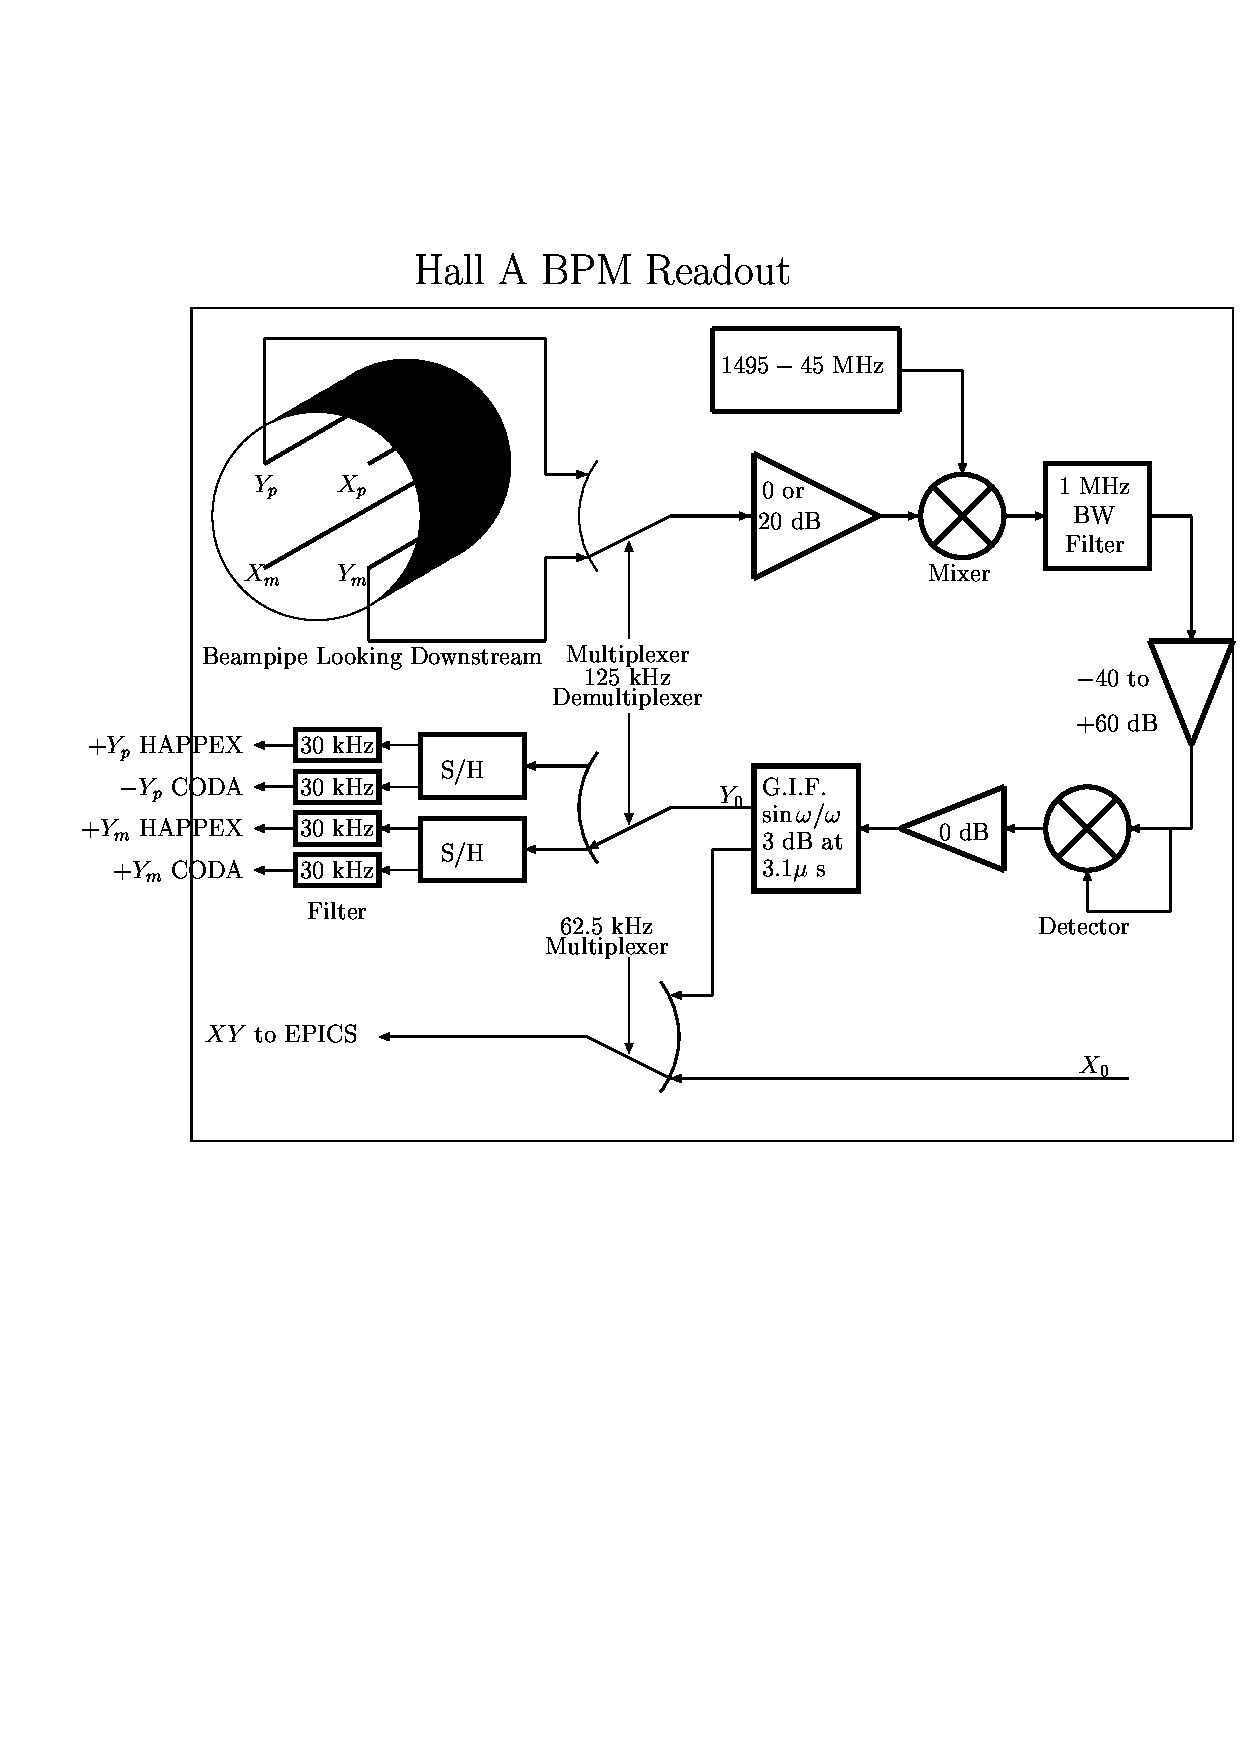
\includegraphics[angle=0,width=15cm]{BPM_fig}
{\linespread{1.}
\caption[Beamline: BPM Readout Electronics]{Schematic of the BPM readout
electronics}
\label{fig:bpmel}}
\end{center}
\end{figure}
}

1. The averaged position over 0.3 seconds is logged into the EPICS~\cite{EPICSwww} database (1 
Hz updating frequency) and injected into the datastream every 3-4 seconds, 
unsynchronized but with an orientative timestamp. From these values we can 
consider that we know the average position of the beam calculated in the EPICS 
coordinate system which is left handed.

2. Approximately once a shift (or more often if requested by the experimenters) 
a B-scope procedure ~\cite{bi:TP} can be performed using the same EPICS electronics 
which then gives the peak-to-peak variation of the beam.

3. Event-by-event information from the BPMs are recorded in the CODA datastream
from each of the 8 BPM antennas (2x4) from which the position of the beam can be 
reconstructed. However, these raw values belong to a parallel electronics chain 
whose constants have to be retrieved by calibrations to the EPICS or scanner 
data. 

\subsection{Beam Exit Channel}

After the target vacuum chamber, which was built by
the University of Virginia, there is an exit beam pipe which 
transfers the scattered beam onto the dump tunnel under vacuum. This exit beam 
pipe is made of a thin walled aluminum spiral corrugated pipe of welded 
construction. The largest diameter is 36 inches with a 0.164 inches wall 
thickness and the smallest diameter is 6 inches with a 0.042 inches wall 
thickness. The whole assembly is rather light (approximately 800 kg) and is 
supported by H shaped adjustable stands. To prevent possible linear collapse 
of the larger diameter sections under vacuum load, four aluminum channels of 
total cross-sectional area of 3'' are welded to its side. A vacuum of 
10$^{-5}$ Torr is maintained with a turbomolecular pump. The exit face of this 
pipe has a 12'' port and is connected to the diffuser with a Beryllium 
window.

}

\section{ Machine/Beamline protection system}
\label{sec:beam-fsd}

The MPS~\cite{MPScebaf} system is composed of the Fast Shutdown System (FSD), Beam Loss 
Monitor (BLM), and gun control system.

The FSD system is a network of permissive signals which terminate at the 
electron gun and chopper 1. The permissive to the gun and chopper
1 may be inhibited by any device connected to an FSD mode. Devices connected to the 
FSD system include vacuum valves, RF systems, Beam loss systems, beam current 
monitors, beam dumps, and particular to Hall A, the target motion mechanism 
and the raster (value and derivative).

The gun control system includes software program which monitors beam 
operating conditions and the state of the FSD and BLM systems. the program 
will warn the operators if a potential for beam damage exists. Potential for 
damage exists when running high average current beam, when FSD nodes are 
masked and when the beam power approaches the operating envelope limits for a 
specific beam dump.

\clearpage
\begin{safetyen}{10}{10}
\section{Safety Information}
\end{safetyen}
}
%
% Information for the ESAD
%

\begin{safetyen}{0}{0}

The beamline in the Hall provide the interface between the CEBAF accelerator
and the experimental hall.   All work on the beamline must be coordinated 
with both physics division and accelerator division; in order to ensure
safe and reliable transport of the electron beam to the dump.

\subsection{Hazards and Mitigations}

All magnets (dipoles, quadrupoles, sextupoles, beam correctors) and beam 
diagnostic devices (BPMs, scanners, Beam Loss Monitor, viewers) necessary for 
the transport of the beam are controlled by Machine Control Center (MCC) 
through EPICS~\cite{EPICSwww}, except for special elements which are addressed in the 
subsequent sections. The detailed safety operational procedures for the Hall 
A beamline should be essentially the same as the one for the CEBAF machine 
and beamline.\\ 

  
\noindent{}Personnel who need to work near or around the beamline should keep in mind the potential hazards:
\begin{itemize}
  \item Radiation ``Hot Spots'' - marked by ARM or RadCon personnel,
  \item Vacuum in the beam line tubes and other vessels,
  \item Thin windowed vacuum enclosers (e.g. the scattering chamber),
  \item Electric power hazards in vicinity of the magnets,
  \item Magnetic field hazards in vicinity of the magnets, and
  \item Conventional hazards (fall hazard, crane hazard etc.).
\end{itemize}

The most hazardous areas along the beamline are roped off it restrict access.   
In particule the scattering chamber, with it's large
volume and thin windows requires hearing protection once it has been evacuated.   
Signs are posted by radcon for any hot spots along the beamline and
radcon must be notified before work is done in a posted area.

Some magnets, as the M{\o}ller spectrometer elements, are covered with plastic
sheets for electric safety. Any access to these magnets requires
the ``Lock and Tag'' procedure~\cite{EHScebaf} and the appropriate training,
including the equipment-specific one. \\

\noindent{}Additional safety information is available in the following documents:
\begin{list}{--}{\setlength{\itemsep}{-0.15cm}}
  \item EH\&S Manual~\cite{EHScebaf};
  \item PSS Description Document~\cite{PSScebaf}
  \item Accelerator Operations Directive~\cite{AODcebaf};
\end{list}

\subsection{Responsible Personnel}

Since the beamline requires both accelerator and physics personnal to maintain
and operate and it is very important that both groups stay in contact that any 
work on the Hall A beamline is coordinated.

\begin{namestab}{tab:beam:personnel}{Beam line: authorized personnel}{%
   Beamline physics division and accelerator divison points-of-contact.}
  \namestabheader{Hall A Physicists}
  \DouglasHiginbotham{\em 1st Contact}
  \RobertMichaels{\em 2nd Contact}
  \namestabheader{Liaisons from Accelerator Division}
  \HariAreti{..to Physics}
  \YvesRoblin{..to Hall-A}
\end{namestab}
\end{safetyen}


\newpage
\section{ Beam Position Monitors}

To determine the position and the direction of the beam on the experimental 
target point, two Beam Position Monitors (BPMs) are located at distances 7.524 m 
(IPM1H03A) and 1.286 m (IPM1H03B) upstream of the target position. 
The BPMs consist of a 4-wire antenna array of open ended thin wire striplines 
tuned to the fundamental RF frequency of 1.497 GHz of the beam ~\cite{bi:bar90}. The 
standard difference-over-sum technique is then used ~\cite{bi:HW} to determine the 
relative position of the beam to within 100 microns for currents
above 1 $\mu $A. The absolute  position of the BPMs can be calibrated with respect to the 
scanners (superharps) which are located adjacent to each of the BPMs (IHA1H03A 
at 7.353 m and IHA1H03B at 1.122 m upstream of the target). The schematic of the 
readout electronics is shown in Figure ~\ref{fig:bpmel}. The
position information from the 
BPMs can be recorded in three different ways:

\begin{figure}
\begin{center}
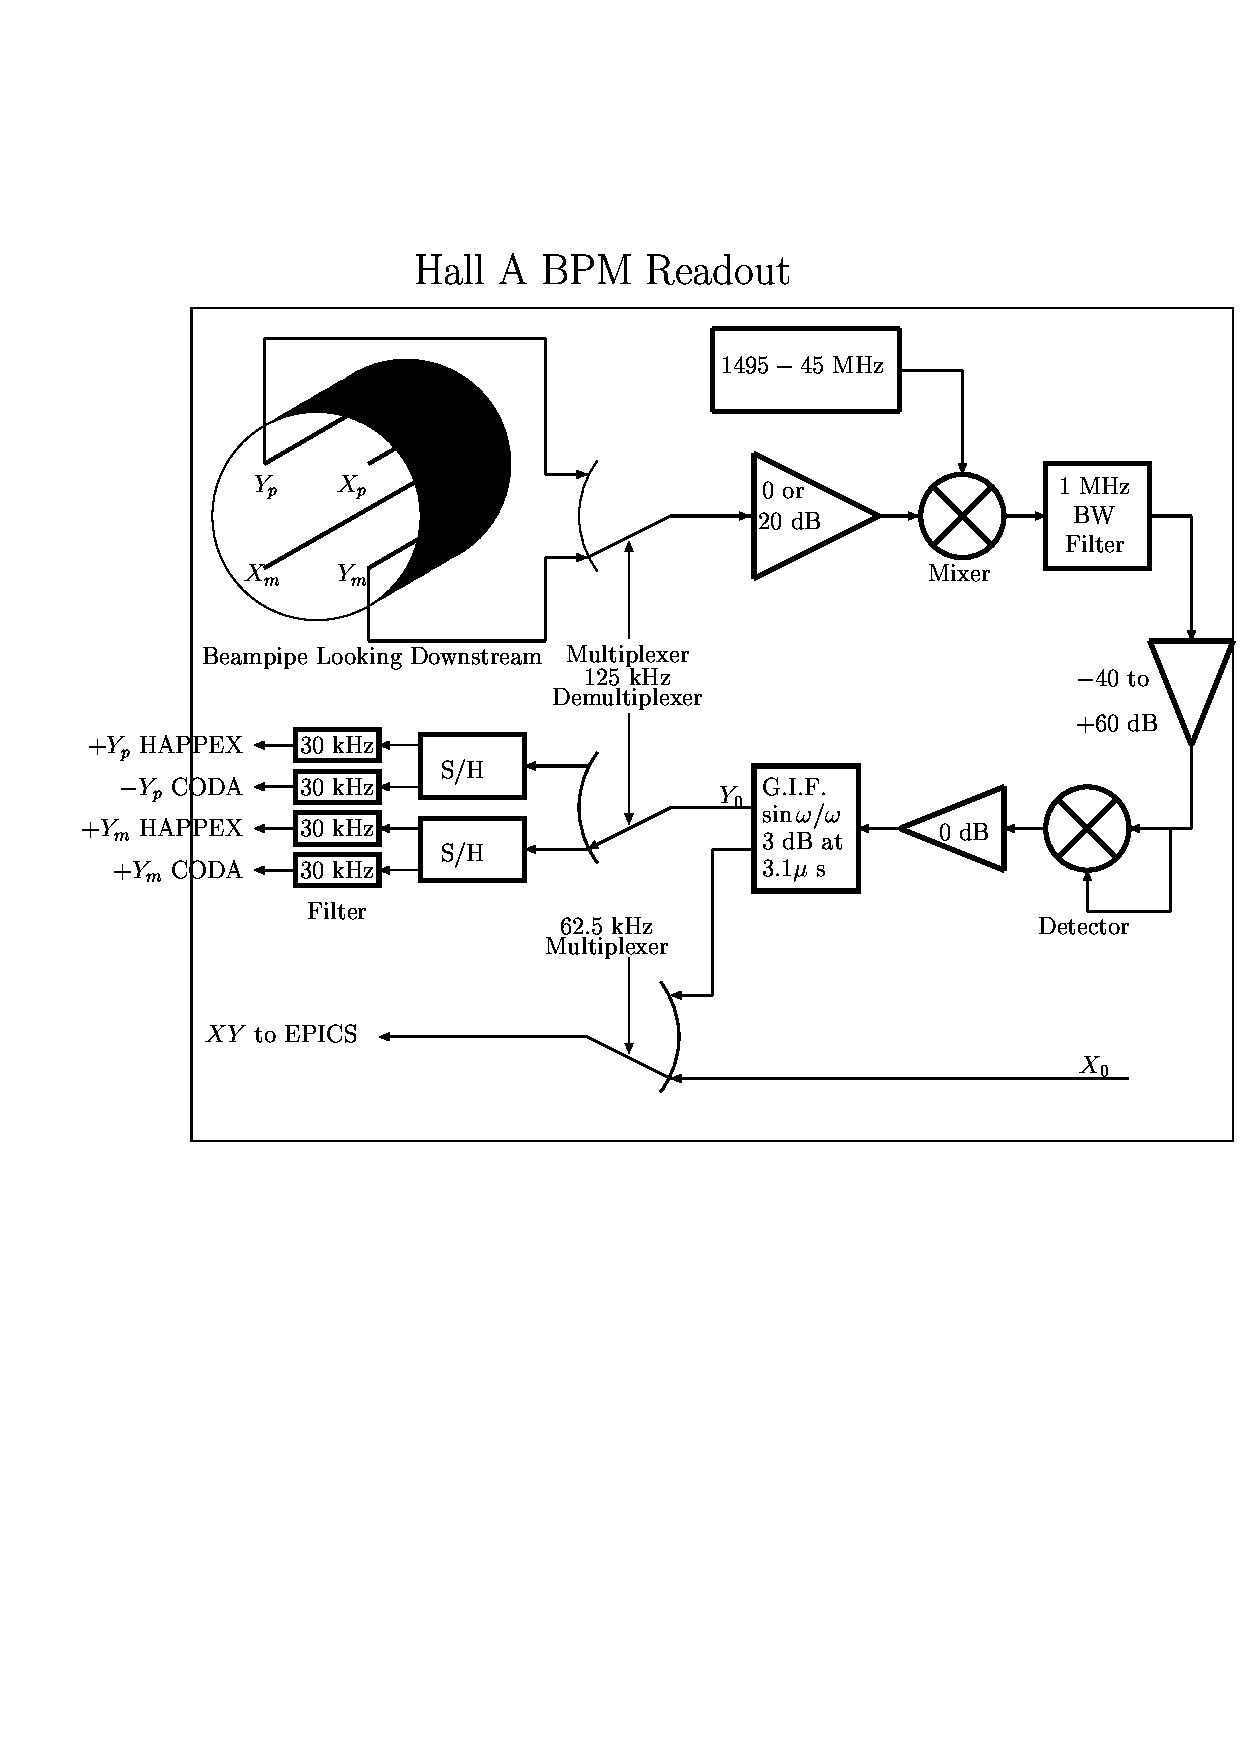
\includegraphics[angle=0,width=15cm]{BPM_fig}
{\linespread{1.}
\caption[Beamline: BPM Readout Electronics]{Schematic of the BPM readout
electronics}
\label{fig:bpmel}}
\end{center}
\end{figure}

\vskip 0.5cm

1. The averaged position over 0.3 seconds is logged into the EPICS database (1 
Hz updating frequency) and injected into the datastream every 3-4 seconds, 
unsynchronized but with an orientative timestamp. From these values we can 
consider that we know the average position of the beam calculated in the EPICS 
coordinate system which is left handed.

\vskip 0.5cm

2. Approximately once a shift (or more often if requested by the experimenters) 
a B-scope procedure ~\cite{bi:TP} can be performed using the same EPICS electronics 
which then gives the peak-to-peak variation of the beam.

\vskip 0.5cm

3. Event-by-event information from the BPMs are recorded in the CODA datastream
from each of the 8 BPM antennas (2x4) from which the position of the beam can be 
reconstructed. However, these raw values belong to a parallel electronics chain 
whose constants have to be retrieved by calibrations to the EPICS or scanner 
data. 


%\begin{thebibliography}{99}
%\bibitem{bi:bar90} W. Barry et al., CEBAF-PR-90-009 (1990).
%\bibitem{bi:HW} C. Hyde-Wright et al., Beam Position Studies for E93050 and priv. comm..
%\bibitem{bi:TP} T. Powers, priv.  comm.. 
%\end{thebibliography}
% ===========  CVS info
% $Header: /group/halla/analysis/cvs/tex/osp/src/beamline/bpms.tex,v 1.1 2003/06/05 17:28:32 gen Exp $
% $Id: bpms.tex,v 1.1 2003/06/05 17:28:32 gen Exp $
% $Author: gen $
% $Date: 2003/06/05 17:28:32 $
% $Name:  $
% $Locker:  $
% $Log: bpms.tex,v $
% Revision 1.1  2003/06/05 17:28:32  gen
% Initial revision
%

\newpage
\section[Beam Current Measurement]{Beam Current Measurement
\footnote{
  $CVS~revision~ $Id: bcm.tex,v 1.5 2003/12/13 06:23:37 gen Exp $ $
}
\footnote{Authors: A.Saha \email{saha@jlab.org}}
}

The Beam Current Monitor (BCM) is designed for stable, low noise, non-intercepting 
beam current measurements. It consists of an Unser monitor, two rf cavities, 
the electronics and a data acquisition system. The cavities and the Unser monitor 
are enclosed in a box to improve magnetic shielding and temperature stabilization.
The box is located 25 m upstream of the target. You can recognize it as a grey 
object on the stands, about 2 m downstream from where the beam enters the 
hall. 

The DC 200 down-converters and the Unser front end electronics are located in Hall 
A. The temperature controller, the Unser back end electronics and its calibration 
current source, cavity's RF unit (housing the RMS-to-DC converter board) and all 
multi-meters, VME crate and computers are located in Hall A control room.

\infolevone{
\subsection{ System Layout}

The schematic diagram of the BCM system is presented in
Fig.~\ref{fig:halla_bcm}.
\begin{figure}[htp]
\begin{center}
\includegraphics[angle=0,width=0.9\textwidth,clip]{habcm_r}
{\linespread{1.}
\caption[Beam Current Measurement: Schematic]{Schematic of the Hall A beam
current measurement system.}
\label{fig:halla_bcm}}
\end{center}
\end{figure}

The Unser monitor is a Parametric Current Transformer designed for non-destructive 
beam current measurement and providing an absolute reference. The monitor is 
calibrated by passing a known current through a wire inside the beam pipe and has a 
nominal output of 4 mV/$\mu $A. It requires extensive magnetic shielding and 
temperature stabilization to reduce noise and zero drift. As the Unser monitor's 
output signal drifts significantly on a time scale of several minutes, it cannot be 
used to continuously monitor the beam current. However, this drift is measured 
during the calibration runs (by taking a zero current reading) and removed in 
calibrating the cavities.  The more stable cavities are then used to determine the 
beam current and charge for each run. We also use the OLO2 Cavity Monitor and the 
Faraday Cup 2 at the Injector section to provide an absolute reference during 
calibration runs.

The two resonant rf cavity monitors on either side of the Unser Monitor are 
stainless steel cylindrical high Q ($\sim 3000$) waveguides which are tuned to the 
frequency of the beam (1.497 GHz) resulting in voltage levels at their   outputs 
which are proportional to the beam current. Each of the rf output signals from the 
two cavities are split into two parts. One part of the signal is  converted to 10 
kHz signals (by the ``downconverters'') and fed into an RMS-to-DC converter board 
consisting of a 50 kHz bandpass filter to  eliminate noise, amplified and split to 
two sets of outputs, which after further processing are recorded in the data 
stream. These two paths to the data stream (leading to the sampled and integrated
data ) will now be described. (The other part of the split signal is downconverted 
to 1 MHz signals and represents the old system (pre Jan 99). Only the HAPPEX 
collaboration presently uses these signals.)

For the sampled (or EPICS~\cite{EPICSwww} or Slow) data, one of the amplifier outputs is sent to a 
high precision digital AC voltmeter (HP 3458A). Each second this device provides 
a digital output which represents the  RMS average of the input signal during that 
second.  The resulting number is  proportional to the beam charge accumulated 
during the corresponding second (or, equivalently, the average  beam current  for 
that second). Signals from both cavity's multi-meters, as well as from the 
multi-meter connected to the Unser, are transported through GPIB ports to the HAC 
computer where they are recorded every 1 to 2 seconds via the data-logging process 
which is described in the calibration procedure. They are also sent through EPICS 
to CODA and the data stream where they are recorded at  quasi-regular intervals, 
typically every two to five  seconds.

For the integrated (or VTOF or Fast) data, the other amplifier output is sent to an 
RMS-to-DC converter which   produces  an analog DC  voltage  level. This level 
drives a Voltage-To-Frequency (VTOF) converter whose output frequency is  
proportional to the  input DC voltage level. These signals are then fed to Fastbus  
scalers and are finally injected into the data stream along  with the other scaler 
information.  These scalers simply accumulate during  the run, resulting  in a 
number which is proportional to the time integrated voltage level and therefore 
more accurately represents the true integral of the current and hence the total 
beam charge. The regular RMS to DC output is linear for currents
from about 5 $\mu$A to somewhere well above 200 $\mu$A.
 Since it is non-linear at the lower 
currents, we have introduced a set of amplifiers with differing gains (x3 and x10) 
allowing the non-linear region to be extended to lower currents at the expense of 
saturation at the very high currents. Hence there are 3 signals coming 
from each BCM (Upx1, Upx3, Upx10, Dnx1, Dnx3, Dnx10). All 6 signals are fed 
to scaler inputs of each spectrometer (E-arm and H-arm) . Hence we have a 
redundancy of 12 scaler outputs for determining the charge during a run. During 
calibration runs we calibrate each of these scaler outputs.   
}

\begin{safetyen}{10}{10}
\subsection{ Authorized Personnel}
\end{safetyen}

All Hall A members are authorized to take BCM calibration data using the Standard 
Non-Invasive Hall A BCM Calibration Procedure. The extended calibration procedures 
involving the Faraday Cup 2 and the OLO2 monitor at the Injector are presently 
performed by A. Saha. 

\vskip 0.2cm

The Accelerator AES group performs the maintenance of the BCM monitors. These 
include:

\begin{tabular}{l l}
1. The Unser calibration. & Every 3 months \\
2. Resonant Cavities Tuning. & Every Downtime \\
3. Multi-meters Autocalibration. & Every Downtime \\
4. Connectors Cleaning. &  Every year \\
5. Unser Keithley Current Source. & Calibration Yearly \\
6. Digital Multi-meters HP3458A and HP 34401A. & Calibration Yearly\\   
\end{tabular}

System Contacts are shown in Table~\ref{tab:BCM:personnel}.
\begin{namestab}{tab:BCM:personnel}{BCM: authorized personnel}{%
   Beam Current Monitor: authorized personnel}
  \ArunSaha{\em Contact}
  \JohnMusson{Accel. expert}
\end{namestab}
%Jean-Claude Denard -x 7555




% ===========  CVS info
% $Header: /group/halla/analysis/cvs/tex/osp/src/beamline/bcm.tex,v 1.5 2003/12/13 06:23:37 gen Exp $
% $Id: bcm.tex,v 1.5 2003/12/13 06:23:37 gen Exp $
% $Author: gen $
% $Date: 2003/12/13 06:23:37 $
% $Name:  $
% $Locker:  $
% $Log: bcm.tex,v $
% Revision 1.5  2003/12/13 06:23:37  gen
% Septum added. Name tables. Polishing
%
% Revision 1.4  2003/12/05 05:48:30  gen
% Polishing
%
% Revision 1.3  2003/06/06 15:19:02  gen
% Revision printout changed
%
% Revision 1.2  2003/06/05 23:29:59  gen
% Revision ID is printed in TeX
%
% Revision 1.1.1.1  2003/06/05 17:28:32  gen
% Imported from /home/gen/tex/OSP
%
%  Revision parameters to appear on the output

\newpage
\section[Fast Raster]{Fast Raster
\footnote{Authors: R.~Michaels \email{rom@jlab.org}}
}


The beam is rastered on target with an amplitude of
several millimeters at 25 kHz to prevent overheating.  
The raster is a set of four of air-core dipoles located
approximately 23 m upstream of the target. 
Two dipoles are for horizontal (X) motion and
another two for vertical (Y).  During the 6 GeV era
there was only one pair of X and Y, but we have doubled
the raster to account for the energy increase to 11 GeV.
The arrangement along the beamline along the 
direction of the beam will be XXYY.

For a typical 40A current in the raster coils, the
deflection by one pair (e.g. the X direction) of coils, 
in radians, is $\theta = 1.94 \times 10^{-3}/ E$
where $E$ is the electron's energy in GeV.
For example, at $E = 6$ GeV, a 0.32 mrad deflection is achieved.
Projected onto the target (about 21 m away) this is a $\pm$ 6.8 mm
excursion {\it if} there were no other magnetic fields 
between the raster and the target; however, there are quadrupoles
which change this depending on the beam tune.

Since 2003 we've used the triangle-wave 
raster pattern designed by Chen Yan.  
This achieves a very uniform rectangular
density distribution of beam on the target 
by moving the beam with a time-varying dipole
magnetic field whose waveform is triangular
with very little dwell time at the peaks.  
The electronics design is an ``H-bridge''
in which switches are opened and closed 
at 25 kHz, to switch between two directions 
of current (100 A peak-to-peak) 
through the raster coils.

Three new features during the 12-GeV era are 
1) the driver of the H-bridge electronics is now
an Agilent model 33522A waveform generator; and
2) The two X are synchronized with each other, and
the two Y are synchronized.  This makes the kicks
add and allows us to accomodate the higher energy
of the beam; and 3) The entire raster can
be synchronized to an external 10 MHz wavetrain
supplied by the polarized injector electronics.
This makes the nominal 25 kHz an exact multiple of
the helicity-flip rate, which achieves a cancellation
of raster noise, important for parity-violation 
experiments only.
The syncrhronization of the pairs of X and Y are
accurate to within a few nsec.

For most users, these three new features will not be
noticeable and the raster will appear to function
the same as during the 6 GeV running.
A user can view the 
status of the raster in the
EPICS overview screen called ``General Accelerator
Parameters'' where the set-point for the radius amplitude
and the readback of the peak-current in the raster are displayed.

Control of the raster is done by first asking the MCC
operators to set up the raster for a particular size
typically 2 mm square.
The control software assumes a field-free region between
the raster and the target, so it is only approximately
correct because there are several quadrupoles in this region.
It is important to check the raster spot size and
make adjustments if necessary.  The adjustment is made
by asking MCC to change the size and noting the 
linear relationship between what their software says
the size is and the actual size.
Relatively small independent adjustments to the 
gains on the X and the Y raster
coils are available in the middle room of the hall A
counting room using the ``PGA Controller'' knobs;
however, it is not recommended to touch these.
Near these knobs is also located an oscilloscope X-Y trace
of the current in the raster.  A fast shutdown (FSD) shuts
the beam down within 0.1 msec if the raster fails, thus
affording some protection of the target.

{\it NOTE:  If you are unsure of the status of the raster,
measure the spot size with very low current ($\le 2 \mu$A) or with
the target out of the beam.}  It would be a mistake
to check the beam spot size with high current on target; by
the time you check it, the target may already be destroyed.
The rastered beam spot on target can be checked with
plots in the ROOT analyzer or by 
using the stand alone code called \mycomp{spot},
also called \mycomp{raster}.
For more details on usage, type \mycomp{spot -h} (help)
on the ADAQ computers.

Regarding the BPM measurements, it should be noted that 
the stripline BPMs displayed by \mycomp{spot} have a high-frequency 
cutoff of approximately 30 kHz.  Since the raster frequency is 25 kHz
the plot of the amplitude distribution shows spikes at the 
limits of the orbit, instead of a flat distribution.  The scale
factor between what is seen in \mycomp{spot} and the real width of the beam
is $\sim 1.5$, i.e. the beam is 1.5 times bigger than the naive
reading of the \mycomp{spot} distribution.



\newpage
% Updated Comments Dec. 2
\infolevone{
\chapter[Arc Energy Measurement]{Arc Energy Measurement
\footnote{Authors: D. Higinbotham \email{doug@jlab.org}}
}
}

\infoleveqnull{
\section{Arc Energy Measurement}
\subsection{Overview}
In order to determine the integral field of the eight dipoles that lead to Hall A, and 
in turn determine the beam energy, a nineth dipole wired in series with the rest is 
located in a special shed near the hall A counting house.
}

\infolevone{
The ARC energy measurement is under EPICS~\cite{EPICSwww} control through 
a MEDM~\cite{MEDMwww} display. Two
independent control systems are used: the beam bend angle measurement through
the arc ("scanners") and the field integral of
the arc ("integral"). To measure the energy: 

\begin{itemize}
\item perform several angle measurements 
\item perform an integral measurement 
\item analyze the integral measurement and note the value of the arc field 
integral 
\item analyze the angle measurements, average the results (proposed by the 
software),
then ask for the energy calculation, enter the above arc field integral and
you will get the beam energy computed from the average angle. 
\end{itemize}

\section{Summary of ARC operations }

Six scanners of the same type, called ``ARC scanner'' and labelled
from scanner \#1 to \#6, are installed on the Hall-A beamline. Scanners \#1
to \#4 are used for the ARC energy measurement and they are located on the Hall-A
arc: \#1 [1HA1C07A] and \#2 [1HA1C07B] just upstream of the arc, in the BSY, and 
\#3 
[1HA1C18A] and \#4 [1HA1C18B] in the Hall-A
tunnel, just upstream the Compton polarimeter. Scanners \#5 [1HA1H03A] and \#6 
[1HA1H03B] 
are located
between the Moller and the target to control the beam geometry on the target
and their use will not be discussed here. 

Procedure for running a harp scan is described elsewhere\footnote{
Harp scan procedure \url{http://hallaweb.jlab.org/equipment/beam/harp_halla/harp.html}.}

Each scanner has a motor/ball-screw/shaft-encoder/vacuum-penetrator system moving
accurately a set of 3 tungsten wires through the beam. Each time a wire crosses
the beam a PMT located a few meters downstream records a signal due to the 
electromagnetic
shower induced by the beam in the wire. Both forward and backward passes are
recorded. The motion is a horizontal translation and, for a forward pass: 

-the translation is from beam left to beam right, 

-the two first wire crossing the beam are at 45deg from the vertical, 

-the third wire, which is the only important for the ARC energy measurement,
is vertical. 

Recording, during the scan, the scanner position and the PMT output voltage
allows us to determine the beam position at each scanner location. Then, using
calibration data not detailed here, we deduce the net beam bend angle through
the arc. This result measured in dispersive arc tuning, along with the field
integral of the arc dipoles, provides an accurate determination of the beam
energy. 

\vspace{0.3cm}

\section{Summary of field integral }

The purpose is to measure absolutely the straight field integral of a 
"BA"
3m long dipole, called the "9th dipole" and located in the
"Dipole Shed". It is of the same type as the 8 arc dipoles
and is powered in series with them. 

The ARC integral setup is basically made of a 3m long plate (the 
"probe")
which is able to move inside the 9th dipole gap along the beam axis and carrying 
two
field measurement devices: a pair of pick-up coils connected in series and a
set of NMR probes. The coils are on both ends of the probe and the NMRs close
to the center. 

-at the "upstream" probe position, the 
"downstream"
coil is close to the dipole center, the "upstream" is outside
the dipole and the NMRs at one end of the dipole: 

Door$<-$-- ....................$<-$-------DIPOLE-----$--->$ 

.............$<-$-------PROBE------$--->$ 

-at the "central" probe position, each coil is at one end
of the 3m long dipole and the NMRs close to the dipole center: 

Door$<-$-- ...................$<-$-------DIPOLE-----$--->$ 

..................................$<-$-------PROBE------$--->$ 

-at the "downstream" probe position, the 
"upstream"
coil is close to the dipole center, the "downstream" is outside
the dipole and the NMRs at one end of the dipole: 

Door$<-$-- ...................$<-$-------DIPOLE-----$--->$ 

....................................................$<-$-------PROBE------$--->$ 

We call upstream the position where the probe is the closest to the shed access
door. Among the 3 above positions, the only one where the NMR can lock on the 
dipole
field is the central one as in the extreme position of the probe, the field 
homogeneity
is not sufficient. The probe position is controlled by a linear encoder. The
Z axis refers to the "beam" direction, increasing from upstream
to downstream. We use three kinds of "Z": 

-Zm to locate a point inside the magnet. The dipole center is at Zm=0 and the
yoke ends at +-1500.mm 

-Zp to locate a point inside the probe. The probe center is at Zp=0. Each of
the 4 NMR probes has a Zp given in the file "magnet.dir".
At a temperature of 21C, the coils are at Zp=+-1519.815mm (from magnet.dir) 

-Zd to refer to a displacement of the probe w.r.t. the dipole. Zd=0 refers to
the upstream (home) position of the probe. The integral measurement is performed
from Zd=0.000mm (1st PDI trigger) to Zd=3199.000mm (last PDI trigger), for forward
pass. Zd is given by the display (at the top of the rack) or by the master screen
("OUT"). 

The relationship between Zm, Zp and Zd is: 

Zd-Zm+Zp=C 

where C is a constant given in magnet.dir (C=1604.000 nomin.). Example of use:
to have the probe center at the dipole center, one must set Zd=1604.000mm (set
Zm=0 and Zp=0 in the above formula, and solve for Zd) 

The integral measurement sequence is the following: 

-from the current position (a priori arbitrary) move the probe upstream, up
to a limit (optic) switch. 

-move downstream by a few mm to cross the encoder index (encoder initialization) 

-move to the central position to measure the central field by NMR, the system
checks if the NMR locks and if the reading is stable, it will be the 
"before"
field 

-move back to upstream position 

-move to downstream position while integrating the flux through the coil system,
this measurement will be called the "forward" integral (duration
\( \sim  \) 7s) 

-move back to upstream position while integrating the flux through the coil
system, this measurement will be called the "backward" integral
(duration \( \sim  \)7s) 

-move to the central position to measure the central field by NMR, the system
checks if the NMR locks and if the reading is stable, it will be the 
"after"
field. 

In addition to the central field, 4 probe temperatures, a local excitation current
measurement, the setting of the dipoles P.S, the readback of the dipoles P.S
and the probe position at NMR measurement time are recorded 
"before"
and "after". 

To perform an integral field measurement: 

1-check if the system works (see "details on integral system 
check"
below) 

2-run the above integral sequence (see "details on integral run"
below) 

3-fix the error(s) if any (see "details on integral errors"
below) 

4-save the data in a file (see "details on integral data save"
below) 

5-analyze the data  


\section{Details on integral run }

To run the integral measurement sequence, call the 
\mycomp{arc\_integral.adl}
medm screen, then: 

-push "start" to start the full sequence 

-look at the results displayed: 

-after the "before" NMR measurement: the 
"before"
data set 

-after the "forward" integral pass: the forward velocity profile
and the forward voltage-after-gain profile 

-after the "backward" integral pass: the backward velocity
profile and the backward voltage-after-gain profile 

-after the "after" NMR measurement: the 
"after"
data set 

-if "BAD NMR" or "PDI saturation" flags
are set, or if something is obviously wrong in the data or plots, call expert. 

-data are ready to be saved (see "Details on integral data save"
below) 


\section{Details on temperatures }

The AC system of the shed is made of two cooling units, a heating unit and a
controller connected to two temperature sensors : one located in the shed and
one located in the BSY. This system is programmed in such a way that the 
temperature
of the shed follows the BSY temperature within +-2C. The BSY temperature can
be anywhere in the 18C to 35C range, regardless of the season. The BSY 
temperature
and the shed temperature are given (in F) by a display panel located close to
the workstation, on the wall. The AC system can be set in manual control by
turning from "auto" to "manual" a set of
switches controlling the cooling units and the heater unit. These switch boxes
are located on the shed wall. If the shed temperature is above 34.4C (94F),
call the crew chief (the electronics can be damaged) and cool down the shed in manual
AC mode. The 4 temperature sensors of the probe are labelled Tx+z+, Tx+z-, Tx-z+,
Tx-z- depending on their position w.r.t. the frame. 

Both "x+" sensors are on the probe edge which is inside the
dipole gap and both "x-" sensors on the opposite edge which
is outside the dipole gap. Both "z-" sensors are at 1/4 of
the long dimension of the probe and both z+ at 3/4 of this length. The average
of the 4 temperatures is used by the analysis program to correct the coil distance
from the thermal expansion of the probe, so it is important to make sure that
the 4 sensors are working well. The user can just make sure that the temperatures
displayed in \mycomp{arc-master.adl} or recorded in 
\mycomp{arc-integral.adl}
are realistic. In \mycomp{arc-integral.adl} they are given in the
order: Tx+z-, Tx+z+, Tx-z-, Tx-z+ Tx-z- and Tx-z+ should be close to the shed
temperature. Tx+z- and Tx+z+ depend on the probe position, as the gap (iron
yoke) is warmer than the shed and the dipole coil (at both ends of the dipole)
is warmer than the iron yoke. For a probe in a central position for more than
about one hour, the Tx+z- and Tx+z+ sensors should give the yoke temperature,
i.e the shed temperature plus 0. to 5.C, depending on the current, LCW temperature
and the magnet/shed temperature history. The 4 temperatures are also displayed
inside the shed, on the electronics rack. These values are digitized by separate
ADCs, so they may differ from the remote values by \( \sim  \)0.1C. 
}

\begin{safetyen}{10}{10}
\infolevone{\section{Shed access and safety }}

Due to the the dipole magnet and motion system, the access to the shed is limited to authorized
persons which are listed in the ESAD and listed below. To be added to the list, 
contact Douglas Higinbotham.
The standard
operation mode of the integral measurement setup is the remote mode, through
the network, from the counting house.
\end{safetyen}

\begin{safetyen}{10}{10}
\infolevone{\section{List of Authorized Personnel for Shed Access}}
\infoleveqnull{\subsection{List of Authorized Personnel for Shed Access}}
\end{safetyen}
\begin{namestab}{tab:arc:personnel}{Arc Energy Measurement: authorized personnel}{%
                 Arc Energy Measurement: authorized personnel}
  \namestabheader{Hall A Personnel}
  \DouglasHiginbotham{\em Contact}
  \namestabheader{Accelerator Personnel}
  \MichaelTiefenback{}
  \YvesRoblin{}
  \RickGonzales{}
  \BillMerz{}
  \MarkAugustine{}
  \HariAreti{}
  \PeteFrancis{}
  \ScottHiggins{}
  \DavidSeidman{}
  \RonLauze{}
  \TonyDay{}
  \ChristopherCurtis{Alignment group}
  \namestabheader{CEA - Saclay experts}
  \PascalVernin{}
  \ChristianVeyssiere{}
  \FrancoisGougnaud{}
  \JacquesMarroncle{}
\end{namestab}



\newpage
\infolevone{
\chapter[Target Chamber]{Target Chamber
\label{sec:target_chamb}
\footnote{
  $CVS~revision~ $Id: tgtcham.tex,v 1.11 2005/04/04 22:27:25 gen Exp $ $
}
\footnote{Authors: ?? \email{??@jlab.org}}
}

The cryo-targets and the waterfall targets 
(see Sec.~\ref{sec:targets-overv}) 
are contained in a special target chamber which is a large 
evacuated  multistaged can. So far, three chambers have been designed:
\begin{list}{\arabic{enumi}.~}{\usecounter{enumi}\setlength{\itemsep}{-0.15cm}}
  \item a chamber used up to 2003;
  \item a chamber designed for use with septum magnets, starting in 2003;
  \item a chamber designed for use with the BigBite spectrometer.
%\footnote{
%        No yet manufactured by Dec,2003.}.
\end{list}

Here, chamber 1 is described. Chambers 2 and 3 are only different in 
size and slightly in shape. The safety considerations fully apply to chambers 2 and 3.
The chamber was designed to isolate the beam line vacuum from  each
HRS so that each HRS could rotate
around the target without vacuum coupling and without jeopardizing
certain desired kinematic and acceptance  specifications of 
both high resolution spectrometers
needed for approved experiments.  It  was also designed to simultaneously
 contain a liquid or gas target and an array of water cooled thin
 metallic foils, both remotely controlled and also be adaptable for
the waterfall target. The desired kinematic specifications that were
 considered included momentum and energy resolution in both arms,
 angular range of spectrometers, angular acceptance, and luminosity.
The chamber vacuum is isolated from the  HRS by using thin aluminum foils. 

The target chamber is designed so that
each spectrometer will have continuous coverage in the standard tune from
$\theta_{min}=$12.54$^\circ$ to $\theta_{max}=$165$^\circ$.
The aluminum window is 6~$in$ high and 0.016~$in$ thick made of 5052 H34 aluminum foil.
The foil forms regularly spaced vertical ridges when
placed under load. The window had an inter-ridge
spacing of 3 inches.
If the window is treated as a collection
of smaller rectangular windows which have the full vertical height
of 6 inches and the inter-ridge spacing as a width,
then stress formulas predict that the 0.016 $in$
material would reach ultimate stress at a pressure higher than 35 PSID
(for both over-pressure and under-pressure). 
There is a gate valve between the 
scattering chamber and the beam entrance (exit) 
pipe. Both 
valves will be closed automatically in the
event that the chamber vacuum begins to rise and an FSD will be caused
( this is done via a relay output of the scattering
chamber vacuum gauge). If either valve is closed an FSD will result.

The target chamber is supported by a 24 $in$ diameter pivot post
secured in concrete, rising about 93.6 $in$ above the Hall A cement floor.
The Hall A target chamber
consists of an aluminum middle ring, a stainless steel base ring,
each with a 41.0 $in$ inner diameter,
and a stainless steel cylindrical top hat with 40 $in$ inner diameter
to enclose the cryotarget and secure the cryogenic connections.

When the scattering chamber is under vacuum, there is a potential
danger of window rupture.
The loud noise from the rupture could hurt
one's ears if not protected. Therefore when the chamber is under vacuum,
protective covers are put on if possible. These must be taken off
for data taking. For restricted access, the protective cover is required
to be on when the chamber is under vacuum. Before switching from controlled
access to restricted access, the protective cover is required to be installed.
Anytime that the scattering chamber
is under vacuum, the pivot area is enclosed in a rope or tape barrier
and a warning sign is posted.
Hearing protection is required in the enclosed area.

\infolevone{
	The aluminum ring with an outer diameter of 45.0 $in$ and
wall thickness 2.0 $in$  is necessary for a sturdy support structure and
to permit machining of the outside surface to accommodate
the flanges for fixed and sliding seals mounted on
opposite sides of the ring that vacuum connect the chamber to each HRS.
The height of the aluminum ring shown is 36.0 $in$, which is
designed to accommodate the mounting flanges.
The stainless steel base ring 
is 11.50 $in$ in height with
one pump-out 6 $in$ diameter port  and with
seven 4 $in$ viewing and electrical feed-through ports.
The base ring will also contain support mechanisms for the solid
target ladder assembly, a rotisserie for collimating slits, radiators, and
magnetic
fingers for
removing the solid target vacuum-lock can. The total height of the top
ring, middle ring, and
base ring is 93.81 $in$. This length is partly determined by our desire to
include with the cryogenic extended target a solid target vertical ladder
secured in an inverted hat through a hole in the base of the chamber.

	The base ring includes an end plate through which the
inverted hat will be adapted to fit into the large vertical pipe serving
as the pivot post for the Hall A spectrometers.

	The stainless steel cylindrical top hat  has
40.0 $in$ inner diameter, and is 0.375 $in$ thick and
46.31 $in$ high , which is necessary to permit the
cryotarget to be withdrawn and to make space available to expose the solid
targets to the electron beam.

   The 200 $\mu$A electron beam, focused to a $\sim$\(0.1\, mm\times
0.1\) mm spot and rastered $\pm$5 mm horizontally or vertically on the
target, enters through a oval hole in the middle ring which
is 2.06 $in$ wide and exits through a 1.81 $in$ hole connected to the
exit pipe.
}

\infolevone{
\section{Target Chamber - Spectrometer Coupling}

   The aluminum middle ring will support a flange on each side for each high
resolution spectrometer. Four flanges will be available: Two flanges will
contain a 6 $in$ window opening which will be covered with a thin foil
(e.g., 10 mil aluminum) .
These two flanges will be used for experiments utilizing
extended  targets that do not require optimum momentum resolution.
The other two flanges will have two fixed ports (with a 8 $in$ $\times$ 6 $in$
opening)
which will be mainly used for calibration of the spectrometers . Fixed ports are
centered at 16.11 $^\circ$ and
45 $^\circ$ for one flange and at 16.11 $^\circ$ and 90 $^\circ$ for the second
flange.

   For a point beam on target a vertical opening in the walls of the chamber
of height 57.15 cm x 0.065 x 2 = 7.43 cm is required so that the scattered
beam is within the full acceptance of the spectrometer.
If the beam is rastered on target $\pm$0.5 cm in the vertical direction,
then the opening in the outer side of the chamber must be at least 8.5 cm for
full acceptance.

From consideration of the angular range of the spectrometers in the standard
tune, the scattered beam acceptance envelope, the effects of an
extended gas target on acceptance,
and the effects of a rastered beam $\pm$ 5 mm on acceptance,
the target chamber requires a window of at least 8.5 cm
high in the aluminum ring extending from 6.33 $^\circ$ (2.48 in) from the
beam exit point to 8.83 $^\circ$ (3.47 in) from the beam entrance point on one
side and a similar window on the other side of the beam.
For future considerations (e.g., using a third arm or sliding seal) the
width of the window on the middle ring was actually constructed
to be 17.78 cm (7 $in$).

\section{Stress Analysis of the Middle Ring}

Since the middle ring has an extensive cut across the midplane on both sides as
well as
entrance and exit holes and loaded with about 25,000 lbs, calculations of the
stresses
 and deformation of  the
midplane support area of the middle ring and deflection of the window opening
were made using the finite element analysis code ANSYS . The work was conducted
by a graduate student in the Department of Civil Engineering at the
University of
Virginia and a REU student.  A scaled down model of the middle ring was
constructed and then tested by applying forces to it using the Materials Testing
Service of the Department of Transportation at the University. ANSYS was first
checked by comparing calculations of the test model deflections to the actual
data. Agreement was  within $\pm$10\%. Results of ANSYS for the target
chamber showed that the maximum deflection of the opening of the window in the
middle ring varied from 0.007 $in$ to 0.015 $in$ depending on how the
middle ring
was loaded. This was decided to be a safe limit. In the final design, several
movable
7 $in$ long, 2 $in$ diameter aluminum support rods are placed in the
window for added support. In addition, flanges defining the ports and
coupling to
the spectrometers can be added, giving additional support to the middle ring.
Compressional stresses, calculated using ANSYS assuming the middle ring was
attached to the
top hat and loaded with 25,000 lbs, were less than 3000 psi 
almost everywhere.
However, stresses over small areas rose to levels 6000 psi near the entrance
and exit holes. These calculations indicated that we did not exceed the safety
limit of 15,000 psi for aluminum. A simple model calculation shown in Appendix
A  gives the result 1434 psi, which represents some average value over the
midplane
contact area.

\section{Vacuum Pumping System}

The vacuum in the target chamber is maintained by an Alcatel ( 880 l/s)
 turbomolecular vacuum pump. The pump is connected to a 6 $in$ port in the
stainless steel ring between 130
 $^\circ \le \theta_p \le 180 ^\circ$. The vacuum pump is
fastened to a horizontal pipe connected to the chamber. The vacuum pressure in
the chamber is about $10^{-5}$ mm. An additional Alcatel pump connected
to an 8 $in$ port should be added to obtain lower vacuum. Both
pumps may be isolated
from the target chamber using gate valves which are remotely operated
from the vacuum control rack and interlocked to the FSD system.


A 2 $in$ all metal gate valve is located between the entrance flange to the
chamber and the beam profile monitor.   
 An additional gate valve is located 2 m downstream of the
 target chamber to isolate the chamber from the exit beam pipe.
}
\begin{safetyen}{10}{15}
\section{Safety Assessment}
\end{safetyen}

The scattering chamber is typically a low maintenance item but it is a vacuum
system and hence problems may occur. The day to day operations of the cryogenic
targets are managed by the Hall A Staff while major maintenance operations are
handled by the Cryogenic Target Group (Physics Division). Occasionally the
cryogenic targets experience difficulties due to failures of the End Station
Refrigerator which supplies the coolant. In these cases the Cryogenics Group
of the Accelerator Division should be contacted.

\noindent{}The target chamber may pose several hazards:

\begin{list}{\arabic{enumi}.~}{\usecounter{enumi}\setlength{\itemsep}{-0.15cm}}
  \item {\bf Rupture of vacuum windows}. This hazard is mitigated by
        lexan guards on the vacuum windows, installed by the hall technicians
        either at the beginning of a ``restricted access'' period 
        %(see Sec.\ref{sec:Access}),
        or during ``control access'', in case an access to the target chamber area is needed.
        Installation and removal of the guards is included in the technician's checklists.
        When the chamber is under vacuum, it is mandatory to use ear protection in the chamber
        vicinity. The appropriate signs must be installed by the technicians. 

  \item {\bf Induced radioactivity}. The RADCON surveyor measures the level of induced
        radiation as a part of the general survey and may declare the target area 
        as ``High Radiation Area'', installing a rope protection around\cite{RWIcebaf}. 

\end{list}

Some other safety issues are discussed in the cryo-target chapter 
(see Sec.~\ref{sec:target-cryo-safety}).
%and also in the polarized target chapter (see Sec.~\ref{sec:target-he3-general}).

\begin{safetyen}{10}{15}
\section[Authorized  Personnel]{Authorized  Personnel}
\end{safetyen}

\begin{namestab}{tab:targ_chamb:personnel}{Target chamber: authorized personnel}{%
      Target chamber: authorized personnel. ``W.B.'' stands for the white board 
      in the counting house.}
  \TechonCall{\em Contact}
  \JessieButler{}
  \DaveMeekins{Target group}
  \JianPingChen{}
\end{namestab}
}

\newpage
\infolevone{\chapter[M{\o}ller Polarimeter]{M{\o}ller Polarimeter}
\setcounter{subsection}{0}}
\infoleveqnull{\section[M{\o}ller Polarimeter]{M{\o}ller Polarimeter}}

The Hall A beam line is equipped with a M{\o}ller 
polarimeter
whose purpose is 
to measure the polarization of the electron beam delivered to the hall. 

\begin{safetyen}{0}{0}

The M{\o}ller Polarimeter system has under gone a major upgrade and an Operational Safety Proceedure (OSP)
is being written and must be reviewed before its use.

\subsection{Hazards and Mitigations}

The hazards and mitigations for this system can be found in the OSP at the end of this document. 

%\infolevone{
%Safety checklist item for this device, located at the end of the beamline section, is solely to ensure
%the beam can be tranported safetly past this system prior to it's recommisioning.
%}

\subsection{Responsible Personnel}
\label{sec:moller-pers}

This list of system experts provided in case there is any question as to the status of system.

\begin{table}[h]
\begin{center}
\begin{tabular}{|ll|l|l|l|l|r|} \hline
  \multicolumn{2}{|c|}{Name} & Dept. & \multicolumn{2}{c|}{Telephone} & 
  \multicolumn{1}{c|}{e-mail} & Comment \\ 
  \cline{4-5}
   &  &   & JLab & Pager &  & \\ 
\hline
 Javier       & Gomez           & JLab    & 7498 & 7498 & gomez@jlab.org    & Primary contact     \\ 
 Oleksandr    & Glamazdin       & Kharkov & 5441 & 5441 & glamazdi@jlab.org &  \\ 
 Viktor       & Gorbenko        & Kharkov & 5441 &   -  & gorbenko@jlab.org &  \\ 
 Roman        & Pomatsalyuk     & Kharkov & 5395 & 0001 & romanip@jlab.org  &  \\ 
\hline
\end{tabular}
\end{center}
\caption[Moller Polarimeter: authorized personnel]{
   The listed name are those who are considered system experts of the Moller Polarimeter and should be contacted
   if there is any question as to the status of the system.
}
\label{tab:moller:personnel}
\end{table}
\end{safetyen}


\newpage
}
% Compton Polarimeter
\infolevone{\chapter[Compton Polarimeter]{Compton Polarimeter}
\label{sec:compton}
\footnote{Author: S.Nanda \email{nanda@jlab.org}}
}
\infoleveqnull{\section{Compton Polarimeter}
\subsection{Overview}}


The Hall A Compton polarimeter has undergone a major upgrade and an
new operational safety proceedure (OSP) is being written and reviewed before the
Compton can be used.   The hazards and mitigations for this system can be found in 
this OSP.

\subsection{Responsible Personnel}

\begin{namestab}{tab:compton:personnel}{Compton Polarimeter: authorized personnel}{%
          Compton Polarimeter: authorized personnel}
 \SirishNanda{Primary Contact}
 \JackSegal{Secondary Contact}
\end{namestab}

\infolevone{
\subsection{Authorized Personnel}

The list
of the presently authorized personnel is given in Table~\ref{tab:compton:personnel}.
Other individuals must notify and receive permission from
the contact person (see Table~\ref{tab:compton:personnel}) to get their names
add to list.

\begin{namestab}{tab:compton:personnel}{Compton Polarimeter: authorized personnel}{%
          Compton Polarimeter: authorized personnel}
 \SirishNanda{\it Contact}
 \JackSegal{Technical}
 \JosephZhang{Optics}
 \MartialAuthier{Engineering}
 \NathalieColombel{Mechanical}
 \PascaleDeck{Electronics}
 \AlainDelbart{Optics}
 \DavidLhuillier{Analysis}
 \YvesLussignol{EPICS}
 \DamienNeyret{DAQ}
 \GerardTarte{Electronics}
 \ChristianVeyssiere{Electronics}
\end{namestab}
}



%
% Old Material
%
% \chapter[eP Beam Energy Measurement]{eP Beam Energy Measurement
\footnote{
  $CVS~revision~ $Id: ep.tex,v 1.6 2003/12/13 06:23:37 gen Exp $ $
}
\footnote{Authors: B.Reitz \email{reitz@jlab.org}}
}
\label{sec:ep}
\section {Purpose and Layout}
\label{sec:ep_purpose}

The Hall A eP system is a stand-alone device to measure the 
energy of the electron beam. It is located along the beamline
17~m upstream of the target. The beam energy $E$ is determined by measuring
the scattered electron angle $\Theta_e$ and the recoil proton angle
$\Theta_p$ in the $^1$H$(e,e'p)$ elastic reaction according to the kinematic
formula:
\begin{equation}
E = M_p \frac{\cos(\Theta_e) + \sin(\Theta_e)/\tan(\Theta_p) - 1}{1 - \cos(\Theta_p)} + O(m_e^2/E^2),
\end{equation}
in which $M_p$ denotes the mass of the proton and $m_e$ the mass of the electron.
The schematic diagram of the eP system is presented in Fig. \ref{fig:ep_layout}. 
Two identical arms, each consisting of an electron and a corresponding proton 
detector system, made up of a set of 2~x~8 silicon micro-strip detectors in the
reaction plane, are placed symmetrically with respect to the beam along the 
vertical plane. The target consists of a rotating CH$_2$ tape.
Simultaneous measurements of the beam energy with both arms result
in cancellation, to first order, of uncertainties in the knowledge of the position
and direction of the beam. 
 \begin{figure}[htb]
    \begin{center}
        \includegraphics*[angle=0,width=0.9\textwidth]{ep_layout}
    \end{center}
    \caption[eP: Layout]{
            Schematic layout of the eP energy measurement system,
            showing the arrangement of its components, the polyethylene (CH$_2$) 
            target, the Cherenkov detectors, the silicon micro-strip detectors (SSD) 
            for protons and electrons, and the scintillator detectors.
            }
    \label{fig:ep_layout} 
 \end{figure}  
%\clearpage

\infolevone{
\section{Description of Components}
\label{sec:ep_desc_comp}

\subsection{High Voltage}
\label{sec:ep_highvoltage}

The eP system is equipped with two gas Cherenkov detectors and 
altogether 18 scintillators. The high voltage for the photomultiplier
tubes of these detectors are provided by a LeCroy 1450 HV power supply,
located in the electronics racks along the beamline. The channel 
assignment and HV voltages (as of summer 2003) are given in
Table \ref{tab:ep_hv}.

\begin{table}[ht]
\begin{center}
\begin{tabular}{|l|r|l|} \hline
Channel & HV (Volts) & Detector  \\ \hline \hline
 1.2 & 2201 & S1 (bottom) \\  \hline
 1.3 & 2200 & S2 (bottom) \\  \hline
 1.4 & 1963 & S1 (top) \\  \hline
 1.5 & 1963 & S2 (top) \\  \hline
 1.8 & 1039 & S3 \\  \hline
 1.9 & 1027 & S3 \\  \hline
 2.0 & 2250 & Cherenkov  \\  \hline
 2.1 & 2250 & Cherenkov  \\  \hline
 3.0 & 1004 & S3 \\  \hline
 3.1 & 1113 & S3 \\  \hline
 3.2 & 1097 & S3 \\  \hline
 3.3 & 1144 & S3 \\  \hline
 3.4 & 1126 & S3 \\  \hline
 3.5 & 1119 & S3 \\  \hline
 3.6 & 1006 & S3 \\  \hline
 3.7 & 1112 & S3 \\  \hline
 3.8 & 1104 & S3 \\  \hline
 3.9 & 1071 & S3 \\  \hline
 3.10 & 1061 & S3 \\  \hline
 3.11 & 1051 & S3 \\  \hline
\end{tabular}
\end{center}
\caption[eP System: HV Summary]{HV connections and HV values. }
\label{tab:ep_hv}
\end{table}

\infolevtwo{
The standard way to control the high voltage is the use of the 
Hall A MEDM~\cite{MEDMwww} graphical user interface (EPICS~\cite{EPICSwww}), which is running 
on the \mycomp{hacsbc2} computer. This computer is located in the counting house,
but can also be accessed from other terminals. Usually at least one terminal 
in Hall A itself has a MEDM screen running, as well. If it is not running, log into \mycomp{hacsbc2}
as user \mycomp{hacuser}, and start the GUI with the command
\mycomp{hlamain}. A screen labeled ``Hall A Main Menu'' will appear (Fig. \ref{fig:medm-hlamain}).
Chose \mycomp{LeCroy HV}, and select \mycomp{Beamline} in the screen which will pop 
up (Fig. \ref{fig:ep_hvlecroy}). 


 \begin{figure}[bht]
    \begin{center}
        \includegraphics*[angle=0,width=6cm]{ep_lecroy}
    \end{center}
    \caption[eP: LeCroy HV Screen]{
	    Epics Menu for the LeCroy High Voltage supplies in Hall A. All slots related
            to the eP system can be accessed from the Beamline button.
            }
    \label{fig:ep_hvlecroy} 
 \end{figure}  
}

For a measurement, all HV channels defined in Table \ref{tab:ep_hv}
should be turned on. The demand voltages in these slots
(Slot 1, Slot 2 ``(e,p) \& ARC'' and Slot 3 ``Moller'') should have 
the correct preset values. 
To turn the HV on (or off), or to change the 
preset values,
press the button below the title of the slot. Another screen will pop-up,
where status and preset values can be adjusted. \infolevtwo{
(See Figs. \ref{fig:ep_hvbeamline}, \ref{fig:ep_hvslot1}, \ref{fig:ep_hvslot2}, and \ref{fig:ep_hvslot3})

\begin{figure}[bht]
    \begin{center}
        \includegraphics*[angle=0,width=0.9\textwidth]{ep_hvbeamline}
    \end{center}
    \caption[eP: Beamline HV Screen]{
	    Overview screen for the high voltage status of devices belonging to the 
            beamline instrumentation.
            }
    \label{fig:ep_hvbeamline} 
 \end{figure}  

\begin{figure}[bht]
    \begin{center}
        \includegraphics*[angle=0,width=0.9\textwidth]{ep_hvslot1}
    \end{center}
    \caption[eP: HV Screen for Slot 1]{
	    Control screen for all high voltage channels from Slot 1.
            }
    \label{fig:ep_hvslot1} 
 \end{figure}  

\begin{figure}[bht]
    \begin{center}
        \includegraphics*[angle=0,width=0.9\textwidth]{ep_hvslot2}
    \end{center}
    \caption[eP: HV Screen for Slot 2]{
	    Control screen for all high voltage channels from Slot 2.
            }
    \label{fig:ep_hvslot2} 
 \end{figure}  


 \begin{figure}[bht]
    \begin{center}
        \includegraphics*[angle=0,width=0.9\textwidth]{ep_hvslot3}
    \end{center}
    \caption[eP: HV Screen for Slot 3]{
	    Control screen for all high voltage channels from Slot 3.
            }
    \label{fig:ep_hvslot3} 
 \end{figure}
}

During a measurement, the alarm handler should be running, so that the 
operator will be informed, should one of the detectors trip. \infolevtwo{This can
also be done manually, by watching the beamline screen Fig. \ref{fig:ep_hvbeamline}.
All fields should be green and showing a voltage close to the values given
in Table \ref{tab:ep_hv}.}
If the EPICS screens are not working, there is an alternative way to 
control the HV, by connecting via telnet directly to the LeCroy 1450.
This can be done from nearly any Linux PC in the counting house with the 
command: \mycomp{$>$ telnet hatsv5 2011}.

%\clearpage

\subsection{MEDM Controls}
\label{sec:ep_medm}

\infolevtwo{
 \begin{figure}[bht]
    \begin{center}
        \includegraphics*[angle=0,width=0.3\textwidth]{ep_slow}
    \end{center}
    \caption[eP: Slow Controls Screen]{
	    EPICS main screen for the controls of the various devices in the eP system. 
            }
    \label{fig:ep_slow} 
 \end{figure} }
The target, the silicon micro-strip detectors, and the setting of the 
Cherenkov detector are controlled by an EPICS GUI \infolevtwo{(Fig. \ref{fig:ep_slow})}. 
It can be started from the ``Hall A Main Menu'' \infolevtwo{(Fig. \ref{fig:medm-hlamain})}
running on \mycomp{hacsbc2} by pressing the \mycomp{EP Energy Measure} button.
(see previous chapter, to learn how to start the ``Hall A Main Menu'' in case
it is not already running)
The controls are actually running on a VME computer \mycomp{hallasc6} 
(Bob calls this \mycomp{e-p~2}). It is located in the eP electronics 
racks along the beamline in Hall A \infolevfour{(Fig. \ref{fig:ep_pic_slow_ctrl})}. This computer
sometimes requires rebooting. \infolevtwo{ The computer is reached through 
the portserver \mycomp{hatsv5} at port 12. To reboot:\\
\\
\mycomp{$>$ telnet hatsv5 2012 \\
user: adaq\\
password: ******* \\
\\ }
if you do not see a prompt, press \mycomp{Ctrl C}.\\
\\
\mycomp{-$>$ reboot}\\
\\
wait for it to finish and then load EPICS:\\
\\
\mycomp{-$>$ $<$ epics \\
...\\
-$>$ Ctrl $]$ \\
telnet$>$ q \\
$>$\\ }

\infolevfour{
 \begin{figure}[bht]
    \begin{center}
        \includegraphics*[angle=0,width=0.75\textwidth]{ep_pic_slow_ctrl}
    \end{center}
    \caption[eP: Picture Slow Controls]{
	    VME crate containing modules for the slow controls of the eP system.
            }
    \label{fig:ep_pic_slow_ctrl} 
 \end{figure}  }
}

\infolevtwo{
\subsection{Silicon Micro-Strip Detectors}
\label{sec:ep_ssd}

There are three GUI's associated with the silicon micro-strip detectors. 
Two of them are important for everyday operations. They are labeled 
\mycomp{MicroStrip Polarization} 
and \mycomp{MX7RH Power Supply and Currents}. To operate the SSDs, pull up
the micro-strip polarization display and turn on all the bias voltages (see Fig. \ref{fig:ep_ssd_bias_control}). 
Make sure that the bias voltages are set to a reasonable value (30 Volts).
Pop up both current strip charts so that you can see when the currents 
have stabilized.
Pull up the MX7RH display and turn on all the supply's (see Fig. \ref{fig:ep_mx7_control}). 
Pop up the power supply strip charts. It takes at 
least 30 minutes for the strips to stabilize.

 \begin{figure}[bht]
    \begin{center}
        \includegraphics*[angle=0,width=0.9\textwidth]{ep_ssd_bias_control}
    \end{center}
    \caption[eP: SSD Bias Voltages Screen]{
            EPICS screen to control the bias voltages for the silicon micro-strip detectors.
            }
    \label{fig:ep_ssd_bias_control} 
 \end{figure}

 \begin{figure}[bht]
    \begin{center}
        \includegraphics*[angle=0,width=0.9\textwidth]{ep_mx7_control}
    \end{center}
    \caption[eP: MX7 Controls Screen]{
	    EPICS screen for the MX7 power supplies. 
            }
    \label{fig:ep_mx7_control} 
 \end{figure}  

%\clearpage
}

\subsection{Target}
\label{sec:ep_target}

The target of the eP system is made of a thin polyethylene (CH$_2$) tape, which 
is moving while it is in the electron beam. \infolevtwo{ To operate the target one has to
pull up the target GUI (Fig. \ref{fig:ep_target_control}). There are two controls, one to start the target moving
labeled \mycomp{Motor Control}
and another labeled \mycomp{Target Motion} to place the target in the beam. 
 \begin{figure}[bht]
    \begin{center}
        \includegraphics*[angle=0,width=0.6\textwidth]{ep_target_control}
    \end{center}
    \caption[eP: Target Control Screen]{
	    EPICS screen for the MX7 power supplies. 
            }
    \label{fig:ep_target_control} 
 \end{figure}  }
The CH$_2$ tape  must always be moving before 
it is placed in the beam. There are two monitors of the tape motion:
an output that shows the motor is powered and a diode-pin combination 
that triggers on a reflective strip. The diodes are often damaged.\\
\begin{safetyen}{10}{5}
Always make sure, that the target is moving while it is in the beam !!!\\
\end{safetyen}
The target movement and motion can also be controlled locally.
\infolevfour{The control box is located under the beamline next to the eP system
(see Fig. \ref{fig:ep_pic_trgtctrl}.)}\\
\begin{safetyen}{10}{5}
If you operate the target manually, make sure that the system
is set back to remote control afterwards.\\
\end{safetyen}
The CH$_2$-tape has only a limited life time. Therefore it
should be exchanged on a regular basis (twice per year, or 
before a long beam time). This work has to be done by the 
Hall A technical staff. 
\infolevfour{
 \begin{figure}[bht]
    \begin{center}
        \includegraphics*[angle=0,width=0.9\textwidth]{ep_pic_trgtctrl}
    \end{center}
    \caption[eP: Picture of Target Control Box]{
	    Control box for the eP target system.
            }
    \label{fig:ep_pic_trgtctrl} 
 \end{figure}  
}
%\clearpage

\subsection{Cherenkov}
\label{sec:ep_cer}

The detectors for the protons (the scintillators S1 and S2, and 
a silicon micro-strip detector) are installed at a fixed angle of
60$^o$. Therefore the scattering angle of the electron varies 
between 9$^o$ and 40$^o$ depending on the beam energy.
There are seven mirrors in each arm, covering the full angular range,
but only one photomultiplier tube per arm, which only looks at one 
mirror at a time. Depending on the beam energy the PMT has to be rotated 
to see the corresponding mirror.
\infolevtwo{ This movement is controlled by the Cherenkov GUI (see Fig. \ref{fig:ep_cer_control}). 
To change the setting, pull up the Cherenkov GUI and 
enter the desired energy in MeV into the widget. One arm at
a time will move. After the first PMT is in position you must re-enter an
energy that is 1 or 2 MeV different in order to move the second PMT.
This is a rather slow process, and can take several minutes.

 \begin{figure}[bht]
    \begin{center}
        \includegraphics*[angle=0,width=0.5\textwidth]{ep_cer_control}
    \end{center}
    \caption[eP: Cherenkov Controls Screen]{
	    EPICS control screen for the Cherenkov detector. User input is only
 	    possible for the beam energy. Be aware that only one detector at a time
            is moved.
            }
    \label{fig:ep_cer_control} 
 \end{figure}  }

The Cherenkov detector is filled with pure CO$_2$-gas. \infolevtwo{The schematic of the gas 
system is shown in Fig. \ref{fig:ep_cer_gas_layout}, \infolevfour{ a picture of the gas-controller
in Fig. \ref{fig:ep_cer_gas_ctrl}}.} The gas-controller is located in the same rack as 
the DAQ system. This rack is located in Hall A next to the beamline.
\infolevtwo{ When performing an eP measurement, the gas system
should be in \mycomp{Pressure}-mode. Therefore the left rotary switch should be at
\mycomp{PRESSION} and the right one at \mycomp{FERME}. The two digital displays
should both indicate a pressure of roughly 10.0~mbar, and the two flow-meters should
be at zero. However the flow regulator under the left flow meter needs to be open.
In this mode the system is pressurized, if the pressure falls below 10~mbar
the automated valve on the gas inlet side opens, until the pressure is restored.
On the other hand, if the pressure rises above 15~mbar, the automated valve in the exit pipe
opens, to release pressure.

If the gas Cherenkov detector needs to be opened, one should turn down the gas flow
on the regulator beneath the left flow meter and open the exit valve (right switch, \mycomp{OUVERT}). 
After the work on the detector is finished,
and the volume is closed again, the detector needs to be set in \mycomp{Flow Mode}.
The left rotary switch needs to be in the \mycomp{DEBIT} and the right one in the
\mycomp{OUVERT} position, the gas flow regulator needs to be opened. After the 
detector is purged for a sufficient time, one should switch back to the \mycomp{Pressure}-mode,
and verify that a pressure of 10~mbar is restored. The CO$_2$ is supplied by the Hall A 
gas system, which also supplies the Cherenkov detectors in the HRS with CO$_2$. The cylinders
and the main vallve (operated manually) are located in the gas-shack.

\begin{figure}[bht]
    \begin{center}
        \includegraphics*[angle=0,width=0.8\textwidth]{ep_cer_gas_layout}
    \end{center}
    \caption[eP: Layout of CO2 Gas System]{
	    Scheme of the gas system for the two carbon dioxide gas Cherenkov detectors.
            }
    \label{fig:ep_cer_gas_layout} 
\end{figure}  

\infolevfour{
\begin{figure}[bht]
    \begin{center}
        \includegraphics*[angle=0,width=0.8\textwidth]{ep_cer_gas_ctrl}
    \end{center}
    \caption[eP: Picture of CO2 Gas Controller]{
            Picture of the gas controller of the eP gas Cherenkov detectors.
            }
    \label{fig:ep_cer_gas_ctrl} 
\end{figure} }
}
%\clearpage

\subsection{Data Acquisition}
\label{sec:ep_daq}

The data acquisition (DAQ) is running on \mycomp{adaqep} in the
\mycomp{epmeas} user account. It is a standard CODA 2.2 system.
The DAQ system also downloads and initializes logic modules,
and thresholds of discriminators. Since these settings depend
on the beam energy, they have to be configured individually for 
each measurement.
\infolevfour{The DAQ hardware itself is located in two racks along the beamline 
in Hall A (see Figs. \ref{fig:ep_pic_daq1}, \ref{fig:ep_pic_daq1}, and \ref{fig:ep_pic_daq3} ). 

 \begin{figure}[bht]
    \begin{center}
        \includegraphics*[angle=0,width=0.75\textwidth]{ep_pic_daq1}
    \end{center}
    \caption[eP: DAQ VME Crate]{
	    VME crate for the eP data acquisition.
            }
    \label{fig:ep_pic_daq1} 
 \end{figure}  
 \begin{figure}[bht]
    \begin{center}
        \includegraphics*[angle=0,width=0.75\textwidth]{ep_pic_daq2}
    \end{center}
    \caption[eP: DAQ NIM Bin]{
	    NIM bin for the eP data acquisition.
            }
    \label{fig:ep_pic_daq2} 
 \end{figure}  
 \begin{figure}[bht]
    \begin{center}
        \includegraphics*[angle=0,width=0.75\textwidth]{ep_pic_daq3}
    \end{center}
    \caption[eP: DAQ CAMAC Crate]{
	    CAMAC crate for the eP data acquisition. 
            }
    \label{fig:ep_pic_daq3} 
 \end{figure}  
%\clearpage 
}

\infolevtwo{
\subsubsection{Trigger-configuration \\ }

Before data taking can start, 
a trigger file appropriate for the nominal beam energy must be created. This
file (\mycomp{settings.conf}) insures that the trigger MLU is programmed 
correctly. You have to be logged into \mycomp{adaqep} as user
\mycomp{epmeas}. There you have to change to the correct directory
(use \mycomp{goconf}) and run a short program (\mycomp{trigger}) to 
generate the trigger file. An example is shown in Fig. \ref{fig:ep_trgcnf}.
Make sure that you give the beam energy in MeV.
The file is read in by CODA during the \mycomp{PRESTART}.

 \begin{figure}[bht]
    \begin{center}
        \includegraphics*[angle=0,width=0.65\textwidth]{ep_trgconfig}
    \end{center}
    \caption[eP: Trigger Configuration]{
	    Example for the generation of a trigger configuration file.
            }
    \label{fig:ep_trgcnf} 
 \end{figure}  

\subsubsection{Rebooting Acquisition-VME \\ }

The DAQ system utilizes a VME computer as its Readout Controller (ROC). This
computer is designated \mycomp{hallasc15} and can be
accessed from the portserver \textbf{hatsv5} at port~2. To reboot it, use the following 
procedure:\\
\\
\mycomp{epmeas@adaqep.jlab.org$>$ telnet hatsv5 2002\\
user: adaq \\
password: ******** \\
}
\\
if you do not see a prompt, press: \mycomp{Ctrl C}\\
\\
\mycomp{-$>$ reboot\\
-$>$ Ctrl $]$ \\
telnet$>$ q \\
epmeas@adaqep.jlab.org$>$\\} 
\\
If the reboot fails, or if CODA afterwards still does not work, 
check that the ROC is configured for CODA 2.2.
Therefore one has to interrupt the reboot by pressing the \mycomp{any}-key.
Press \mycomp{p} to show the present setting, it should look the following
way:\\
\\
\mycomp{boot device          : ei \\
processor number     : 0 \\
host name            : adaqs3-ep.jlab.org \\
file name            : /home/epmeas/vxworks/vx162lc-8MB \\
inet on ethernet (e) : 129.57.188.14:ffffff00 \\
inet on backplane (b): \\
host inet (h)        : 129.57.164.45 \\
gateway inet (g)     : 129.57.188.1 \\
user (u)             : epmeas \\
ftp password (pw) (blank = use rsh): \\
flags (f)            : 0x20 \\
target name (tn)     : hallasc15 \\
startup script (s)   : /home/epmeas/vxworks/epmeas\_22.boot \\
other (o)            : \\
}
\\
Press \mycomp{c} to change these settings and 
reboot the ROC by pressing \mycomp{@} afterwards.

\subsubsection{Running CODA \\ }

To run CODA, you have to be logged into \mycomp{adaqep} as user
\mycomp{epmeas}. From the prompt CODA can be started with the
command \mycomp{runcontrol}. Withing CODA you have to click 
on \mycomp{Configure} and choose configuration \mycomp{epm1},
then click on \mycomp{Download}, and finally on \mycomp{Prestart}.
At this point the information in the settings.conf file,
 that controls the acquisition
(thresholds, discriminator widths, and trigger MLU logic) is downloaded to the
hardware and spooled to the diagnostics window. This provides an opportunity
to check this information.

The actual data taking starts after pressing \mycomp{Go}. The rate 
is usually rather low, below one per second. However if after 
a few minutes the number of events is not increasing, one has to 
verify if:
\begin{itemize}
\item the trigger is programmed correctly,
\item all components of the DAQ are running,
\item the Cherenkov is at the correct position,
\item the target is in the beam and moving.
\end{itemize}
After collecting enough data, the \mycomp{End} button should be used
to end data-taking, and to ensure that all data is written into the 
datafile.

\subsection{Data Analysis}
\label{sec:ep_analysis}

The data analysis is currently done in two steps, using
two different programs. Both run on \mycomp{adaqep} in the
\mycomp{epmeas} account.

In the first step, the CODA raw file is converted into an
ASCII file.
For this part of the analysis one has to change to the \mycomp{epcoda}
directory, which can be done by typing \mycomp{goep}, and start
the program \mycomp{eplong}:\\
\\
\mycomp{epmeas@adaqep.jlab.org$>$ goep \\
epmeas@adaqep.jlab.org$>$ eplong \\
~How many events (-1= lots) ? \\
-1 \\
~What file name ? \\
epmeas02\_\#\#\#.dat \\
~What output filename ? \\
\#\#\# \\
~opening/adaqep/data1/epraw/epmeas02\_\#\#\#.dat    \\
\\
~Have opened  epmeas02\_\#\#\#.dat \\
\\
~bank length is wrong \\
~bank length is wrong \\
~Finished;  events read =   234 \\
epmeas@adaqep.jlab.org$>$  \\
}
\\
In this example \#\#\# is the three-digit CODA run number. \mycomp{eplong} can be started,
while CODA is still taking data for that run.

The second step of the analysis utilizes a stand-alone analysis code,
which asks for nominal beam energy, beam position, beam intensity
and duration and uses the output of \mycomp{eplong}. One has to
change into the \mycomp{ep} directory and start the code:\\
\\
\mycomp{epmeas@adaqep.jlab.org$>$ cd \\
epmeas@adaqep.jlab.org$>$ cd ep \\
epmeas@adaqep.jlab.org$>$ ep \\
}
\\
Make sure, that the nominal beam energy is given in \textbf{GeV}.
The program prints the result for the energy, together with
the path and name for log-files and ntuple files.
It is recommended to repeat the analysis with a slightly changed
nominal energy value or with slightly changed cuts, to verify that
the automatic fitting procedure does really find the eP events,
and does not trigger on noise. One also has to be aware, that one
needs elastic events in both arms to get a reliable results.
Furthermore, for beam energies between 2.7~GeV and 3.4~GeV,
where micro-strip detector E$_3$ is used, the obtained
values are systematically shifted as compared to the results from the ARC energy measurements, 
probably due to a misalignment of this detector.
}}

\infolevtwo{
\section{Operating Procedure}
\label{sec:ep_ops_proc}

In preparation of an eP measurement, the mirrors of the Cherenkov 
should be driven to the appropriate position (see Sec. \ref{sec:ep_cer}), 
and the silicon micro-strip detectors should be turned on (see Sec. \ref{sec:ep_ssd}).
These two measures should be started several hours before the actual 
eP measurement is scheduled.

Shortly before the measurement, the high voltages for the scintillator photomultiplier tubes
and for the Cherenkov photomultiplier tubes need to be turned on (see Sec. 
\ref{sec:ep_highvoltage}). Finally the DAQ should be 
prepared (see Sec. \ref{sec:ep_daq}).

For the eP measurement, the following requirements need to 
be communicated to MCC:
\begin{itemize}
\item 3-4 $\mu$A CW beam 
\item Raster OFF
\item OTR target 1C12 OUT
\item Physics target empty ( or be able to stand unrastered, uncentered beam )
\item Centered on BPM 1H01 absolute
\item Fast Feedback must be ON
\end{itemize} 
To check the beam position (recommended!), you can use the 
\mycomp{Monticello} screen from MCC, which is usually also available
on one monitor in the Hall A counting house. On the 
\mycomp{Monticello} main menu
select \mycomp{BPM}, and there click on
\mycomp{BPM Spikes and Position Summary}.
This will pop up a new screen, go to the top row of this screen 
(\mycomp{``Injector, BSY, Hall A, B and C Transport''}) 
and select \mycomp{Pos Sum}.  From here select \mycomp{Hall A Transport}.
A screen will show up, which summarizes beam positions at various 
locations. For the eP system the numbers in \mycomp{BPM 1H01 absolute}
are the only ones relevant.

When MCC has established those conditions, the high voltages and 
the micro-strip detectors should be checked one more time.
Next the eP target tape motion should be turned on 
(\mycomp{Motor Control}) and then the 
target can be moved into the beam (\mycomp{Target Motion}, 
see Sec.\ref{sec:ep_target}.)

Now the actual data-taking can start, by pressing \mycomp{Prestart/Go}
in the CODA runcontrol screen. The rate should be a few 
tenth of a Hz. If the BPM position changes, the fast feedback system fails, or a 
lot of beamtrips accrue, consider stopping the run and starting a new 
one.

One should analyze the data, while CODA is still running. 
With a hundred events one can already check the quality of the 
data, and estimate how much more statistics are needed.
Typically one needs 40-50 minutes of stable beam or a few 
hundred events.

After data taking is finished, and it is verified, that there
is a sufficient number of events to extract a number for the beam energy, 
the following steps should be taken:
\begin{itemize}
\item eP target: should be moved out of the beam
\item eP target: motor should be turned off (after it is moved out)
\item MCC can restore the beam needed for the experiment: 
\begin{itemize}
\item restore beam position at target
\item restore raster
\item insert OTR 1C12, if needed for the experiment
\item restore beam current
\end{itemize}
\item Shift workers can go back to physics target
\item high voltages for eP scintillators and eP Cherenkov should be turned off
\item MX7 power supplies and micro-strip bias voltages should be turned off
\item CODA windows should be closed
\item remaining windows from the \mycomp{epmeas} account should be closed
\end{itemize}
Before posting the result of the eP measurement, one should make sure,
that the full statistics of the run is analyzed, that the result is 
independent of the chosen cuts, and that there are events on both 
arms of the eP system.

\section{Maintenance}
\label{sec:ep_maintenance}

The CH$_2$ tape of the eP target 
should be exchanged on a regular basis (twice per year, or 
before a long beam time). This work involves opening the 
eP scattering chamber and therefore breaking the vacuum in
this section of the beamline. This work has to be coordinated
by the Hall A work coordinator, and can only be done by the 
Hall A technical staff personnel. 
}

\begin{safetyen}{0}{0}
\section {Safety Assessment}
\label{sec:ep_safety}

\subsection{High Voltage}

The LeCroy 1450~HV~crate equipped with LeCroy~1461N
high voltage cards provides up to 3~kV of low current power.
RG-59/U~HV~cables, certified for up to 5~kV, with standard SHV 
connectors are used to connect the power supply to the photomultipliers.
The PMTs for S1,S2 and for the Cherenkov detector are usually operated 
at 1900~-~2300~V and draw up to 1.5~mA currents. The PMTs for the 
S3 scintillators are operated at 1000~-~1150~V, drawing 0.9~mA current.
The high voltage MUST be turned off during all work on the detector.

\subsection{Silicon Micro-Strip Detectors}

The SSD are prone to radiation damage, regardless if they are 
turned on or off. Ion chambers next to the eP measure radiation levels
in this part of the beamline and interrupt beam delivery via the
fast shutdown system (FSD), in case the levels are not acceptable. Therefore these
ion chambers should never be masked. 

\subsection{Target}

The target is controlled by the experimenters, not by MCC. Therefore it is
the responsibility of the eP operator to ensure that it is properly
operated.
To avoid damage to the eP target, the following instructions have to be 
followed:
\begin{itemize}
\item The target should only be in the beam during an eP measurement
\item Before inserting the target into the beam, the tape motion has to
be turned on. The target should not be in the beam when the tape is not moving. 
\item The target should not be in the beam 
if the beam current is greater than 5 $\mu$A. 
\item After finishing the eP measurement, the target should be moved out
of the beam, and then the tape motion stopped. 
\item The tape should not run, and the target should not be in the beam
without an eP operator being present.
\end{itemize}

\subsection{Cherenkov}

If for work on the Cherenkov detector the detector needs to be opened, 
the CO$_2$ gas flow needs to be stopped. After the work is finished the 
detector needs to be purged and later the operating mode needs to be restored.
\infolevone{(see Sec. \ref{sec:ep_cer})}

\end{safetyen}

% include the personnel list
\begin{safetyen}{0}{0}
\subsection[List of Authorized  Personnel]{List of Authorized  Personnel
\footnote{
   $CVS~revision~ $Id: ep-personnel.tex,v 1.1 2003/11/18 22:34:49 reitz Exp $ $
 }
\footnote{Authors: B.Reitz \url{mailto:reitz@jlab.org}}
}
\end{safetyen}
%All authorized persons must sign next to the correct listed
%name. This signature indicates that they have read and understand this
%OSP.
The list
of the presently authorized personnel is given in Tab.~\ref{tab:ep:personnel}.
Other individuals must notify and receive permission from
the contact person (see Tab.~\ref{tab:ep:personnel}) before adding their names 
to the above list.
\begin{table}[ht]
\begin{center}
\begin{tabular}{|ll|l|l|l|l|r|} \hline
  \multicolumn{2}{|c|}{Name} & Dept. & \multicolumn{2}{c|}{Telephone} & 
  \multicolumn{1}{c|}{e-mail} & Comment \\ 
  \cline{4-5}
   &  &   & JLab & Pager &  & \\ 
\hline
 {\em Bodo} & {\em Reitz}  & JLab    & 5064 & 5064 & reitz@jlab.org      & Contact     \\ 
 Pierre     & Bertin       &         & 7544 & 5035 & bertin@jlab.org &  \\ 
 Ed         & Folts        & JLab    & 7857 & 7857 & folts@jlab.org  &  eP-Target \\ 
 Jack       & Segal        & JLab    & 7242 & 7242 & segal@jlab.org  &  Gas System \\ 
\hline
\end{tabular}
\end{center}
\caption[eP System: authorized personnel]{
   eP System: authorized personnel. The primary contact person's
   name is marked with a slanted font. 
}
\label{tab:ep:personnel}
\end{table}

% ===========  CVS info
% $Header: /group/halla/analysis/cvs/tex/osp/src/beamline/ep-personnel.tex,v 1.1 2003/11/18 22:34:49 reitz Exp $
% $Id: ep-personnel.tex,v 1.1 2003/11/18 22:34:49 reitz Exp $
% $Author: reitz $
% $Date: 2003/11/18 22:34:49 $
% $Name:  $
% $Locker:  $
% $Log: ep-personnel.tex,v $
% Revision 1.1  2003/11/18 22:34:49  reitz
% personnel for eP system
%
% Revision 1.1.1.1  2003/06/05 17:28:27  gen
% Imported from /home/gen/tex/OSP
%


% ===========  CVS info
% $Header: /group/halla/analysis/cvs/tex/osp/src/beamline/ep.tex,v 1.6 2003/12/13 06:23:37 gen Exp $
% $Id: ep.tex,v 1.6 2003/12/13 06:23:37 gen Exp $
% $Author: gen $
% $Date: 2003/12/13 06:23:37 $
% $Name:  $
% $Locker:  $
% $Log: ep.tex,v $
% Revision 1.6  2003/12/13 06:23:37  gen
% Septum added. Name tables. Polishing
%
% Revision 1.5  2003/12/08 15:34:23  reitz
% change paragraph to subsubsection
%
% Revision 1.4  2003/12/05 05:48:30  gen
% Polishing
%
% Revision 1.3  2003/11/18 22:34:16  reitz
% personnel added
%
% Revision 1.2  2003/11/17 06:50:16  gen
% CVS records added
%
 eP device has been removed from Hall A
% \section[Bremsstrahlung Radiator]{Bremsstrahlung Radiator
\footnote{
  $CVS~revision~ $Id: radiator.tex,v 1.6 2003/12/13 06:23:37 gen Exp $ $
}
\footnote{Authors: A.Saha \email{saha@jlab.org}}
}

\subsection{Overview}

The Bremsstrahlung radiator is the last element in the Hall A beam line 
before the scattering chamber, and is about 72.6 cm from the center 
of the physics targets.
Its design is based on the Hall C radiator 
system built by David Meekins, and documented in the Hall C operations
manual.

The central component of the system is a U-shaped, oxygen-free copper target
ladder, with six positions for differing thicknesses of oxygen-free Cu foils.
The ladder is designed so that it never intersects the beam.
The 3.175-cm wide gap in the ladder is spanned only by 
the target foils, which are 6.35 cm wide, 3.175 cm high,
and 3.332 cm apart (center to center).
A stepper motor moves the target ladder with foils up and down,
into and out of the beam.
Hard stops prevent motion of the ladder beyond the limit switches.
Water cooling of the radiator ladder cools the foils, preventing
damage from overheating by the beam.

The interaction of the beam with the foils produces
background radiation in the Hall.
%At 3 GeV, ion chamber trip levels do not need to be
%adjusted, and increases in detector background rates are minimal;
%further tests are planned for 0.8 GeV.
For normal operation of the radiator, currents of 30-50 $\mu$A and energies 
above 1 GeV, ion chamber trip levels do not need to be adjusted. At energies 
below 1 GeV, it might be desirable to use lower beam currents or thinner 
radiatior foils. 
No local shielding is installed, as calculations indicate
that this will not significantly affect dose at the site boundary.
Any installation and/or subsequent modifications must be coordinated
with RadCon.

\begin{safetyen}{10}{10}
\subsection{Safety Issues}
\end{safetyen}

The only safety issue concerning the Bremsstrahlung radiator is that of
induced radioactivity in the Cu targets and in the water 
used for cooling the targets.
The water cooling system is a closed loop,
using a portable welding-torch water cooler, located
under the beam line just upstream of the target. 
The cooler is kept in a tray which is intended to provide secondary
containment in case of a leak.
The cooling system must not be breached or drained without concurrence from 
the RCG. Accidental breach or spill constitutes a radiation contamination 
hazard.  
A spill control kit, capable of containing a system leak or spill, is
staged by the door to the hall. In the event of a spill notify
the RCG.

\infolevtwo{
\subsection{Operations}

Although the radiator foils are water cooled, a high current electron beam
may melt the foils.
Beam currents with the radiator will be limited to 30 micro-amperes.
Including a safety factor, the raster radii given in Table 1
will limit the temperature rise to 100 $^{\circ}$C.

\begin{table}
\begin{center}
\caption[Bremsstrahlung Radiator: Raster Radius]{Raster radius as a function of 
beam current.}
\begin{tabular}{cc}
\hline
\hline
Current ($\mu$A) & Minimum raster radius (mm) \\
\hline \\
10 & (not needed) \\
15 & 0.2 \\
20 & 0.7 \\
25 & 1.3 \\
30 & 2.1 \\
\hline \hline \\
\end{tabular}
\end{center}
\end{table}

The only operational control consists of moving the ladder in and out.
Radiator position is determined by the ratio of the readback voltage from 
a linear encoder to the voltage applied to it.
Table 2 gives the radiator position as a function of this ratio.
The foil thicknesses are set so that the thickness, in percent
of a radiation length, equals the foil number, except that
no foils are mounted in position 1.

\begin{table}
\begin{center}
\caption[Bremsstrahlung Radiator: Encoder Calibration]{Encoder voltage 
calibration. See text.}
\begin{tabular}{ccc}
\hline
\hline
Position & Voltage ratio & $V_{\rm encoder}$ for $V_{\rm supply}$ = 5 V \\
\hline \\
out limit & 0.030 & 0.15 \\
 foil 1 & 0.102 & 0.511 \\
 foil 2 & 0.269 & 1.346 \\
 foil 3 & 0.436 & 2.179 \\
 foil 4 & 0.603 & 3.013 \\
 foil 5 & 0.769 & 3.847 \\
 foil 6 & 0.936 & 4.681 \\
 in limit & 0.966 & 4.831 \\
\hline \hline \\
\end{tabular}
\end{center}
\end{table}

Software controls of the ladder position are under development;
radiator position is changed by calling
MCC and requesting that the radiator be set to some foil position,
or to the out limit.
The position may be changed with beam on.
A manual-control backup system also exists.

Both software and manual backup systems
control an Oregon Micro Systems MH10DX step motor driver,
which drives a Slo-Syn M063-LS09 stepper motor.
The MH10 driver, power supplies, and other control circuitry, 
are in a custom-built box located in the hall in rack 1H75B10.
The linear encoder voltage ADC is in slot 5 of the CAMAC crate in 
rack 1H75B02; radiator inputs use channels 15 and 16, and
are connected through a patch panel to block 30 in rack 1H75B08.

When the radiator is not being used, the system should be set to the
out-limit position, so that it is clear of the beam.
Power to the control box in the hall may be turned off with a front-panel 
switch if the radiator will not be used for a long time - and should be 
turned off if work is to be done on the radiator.
This deactivates the limit switches and the linear encoder, 
but does not affect positioning.
Additional hard stops should be installed as a safety measure.
The Hall A technical staff checklist, done as part of preparations for
closing the Hall for beam, includes checking the radiator
position, the status of the control box, and the installation of hard stops.

\subsection{Special Instructions}

Care must be taken in case any removal or disassembly of the radiator
system is needed.
Disconnecting the stepper motor from the motor driver
while power is on can damage the motor, motor driver, and VME44 board.

The Cu targets will certainly be activated in the course of an experiment.
Therefore, only remove the Cu target, the target ladder,
and/or the whole radiator system in the presence of a Radcon officer.

Ron Gilman should be informed in case of any problems with the radiator.
Except for normal operations of the radiator, any work on the
system hardware requires that RadCon has concurred in the work and
either Ron Gilman or David Meekins is present.

}
% ===========  CVS info
% $Header: /group/halla/analysis/cvs/tex/osp/src/beamline/radiator.tex,v 1.6 2003/12/13 06:23:37 gen Exp $
% $Id: radiator.tex,v 1.6 2003/12/13 06:23:37 gen Exp $
% $Author: gen $
% $Date: 2003/12/13 06:23:37 $
% $Name:  $
% $Locker:  $
% $Log: radiator.tex,v $
% Revision 1.6  2003/12/13 06:23:37  gen
% Septum added. Name tables. Polishing
%
% Revision 1.5  2003/12/10 21:00:22  saha
% brem
%
% Revision 1.4  2003/12/05 05:48:30  gen
% Polishing
%
% Revision 1.3  2003/06/06 15:19:03  gen
% Revision printout changed
%
% Revision 1.2  2003/06/05 23:29:59  gen
% Revision ID is printed in TeX
%
% Revision 1.1.1.1  2003/06/05 17:28:32  gen
% Imported from /home/gen/tex/OSP
%
 currenlty not used
%

%
% Beamline Material for Operations Manual and ESAD
%
\infolevone{\part{Beamline}}
%\infoleveqnull{\chapter{Beamline}}

\graphicspath{{beamline/figs/}}
\renewcommand{\dirfig}[0]{beamline/figs}
\renewcommand{\dircur}[0]{beamline}

\infolevone{
\infolevone{
\chapter[General Description]{General Description
\footnote{Authors: D. Higinbotham \email{doug@jlab.org} with many thanks to A.Saha$^{Deceased}$}}
\section{Introduction}
\label{sec:beam-intro}
}
\infoleveqnull{\section{Beamline}}

\infolevone{
The control and measurement equipment along the Hall A beamline consists of 
various elements necessary to transport beam with the required specifications 
onto the reaction target and the dump and to simultaneously measure the 
properties of the beam relevant to the successful implementation of the 
physics program in Hall A.  The resolution and accuracy requirements in Hall 
A are such that special attention is paid to the following:
\begin{list}{\arabic{enumi}.~}{\usecounter{enumi}\setlength{\itemsep}{-0.15cm}}
  \item Determination of the incident beam energy;
  \item Control of the beam position, direction, emittance and stability;
  \item Determination of the beam current;
  \item Determination of the beam polarization.
\end{list}

A schematic of the Hall A line starting at the shield wall is
shown on Fig.~\ref{fig:Aline1},~\ref{fig:Aline2} and \ref{fig:Aline3}. 

\begin{figure}
\begin{center}
\includegraphics[angle=0,width=15cm]{compton_r}
\caption[Beamline: Hall A Beamline Overview]{Schematic of the Hall A beamline
starting at the shield wall to end of alcove.}
\label{fig:Aline1}
\end{center}
\end{figure}

\begin{figure}
\begin{center}
\includegraphics[angle=0,width=15cm]{aline}
\caption[Beamline: Hall A Beamline Overview]{Schematic of the Hall A beamline
from the end of the alcove to the target chamber.  This image has been updated
to show the new larger raster system as well as the new Moller magnets.}
\label{fig:Aline2}
\end{center}
\end{figure}

\begin{figure}
\begin{center}
\includegraphics[angle=0,width=15cm]{dump_r}
\caption[Beamline: Hall A Beamline Overview]{Schematic of the Hall A beamline
from the target chamber to the dump diffuser.}
\label{fig:Aline3}
\end{center}
\end{figure}

\obsolete{
\section{Beam Line Components}
\label{sec:beam_line_comp}

The main components of the basic Hall A beamline are described
in this section.
Table~\ref{tab:beam_tab1} gives a listing of all the various elements
along the Hall A beamline from the switch yard to the dump.

%\vspace*{0.5cm}
\begin{longtable}[hpt]{lllllr}
\hline
Girder & Diagnostic & Optics & Valves & Element & Distance (m) \\
\# & Elements & Elements & \& Pumps & \# & from target \\ \hline
\multicolumn{6}{c}{{\bf Beam Switch Yard}} \\ \hline 
& TV Viewer &&&ITV2C00 & 148.12862 \\ 
1CB2 & & Dipole (2.3m + & & MLA1C02 & 146.60000 \\
&&0.13m shim) &&& \\
1CB3 && BD && MBD1C00V & 144.18700 \\
&&&Valve & VBV1C00A & $\sim$142.78686 \\
& Current &&& SBC1C00 & $\sim$136.99564 \\
& Beam Stopper &&& SSS1C00 & $\sim$136.53844 \\
& Beam Stopper &&& SSS1C00A & $\sim$136.08124 \\
1C01 & BPM &&& IPM1C01 & 134.32465 \\
&& BC && MQA1C01 & 133.95000 \\
&&& Ion Pump & VIP1C01 & 133.04195 \\
1C02 & BPM &&& IPM1C02 & 132.02465 \\
&& BC && MQA1C02 & 131.65000 \\
&&&& MBC1C02V & 131.30685 \\
1C03 & BPM &&& IPM1C03 & 129.02465 \\
&& BC && MQA1C03 & 129.35000 \\
&&& Ion Pump & VIP1C03 & \\
&&& Rough Pump & VRV1C03 & 128.44195 \\
&&& Convectron & VTC1C03 & \\
1CB4 && Dipole (1m) && MBN1C04 & 116.70000 \\
1C04 & BPM &&& IPM1C04 & 115.42465 \\
&& Quad && MQA1C04 & 115.05000 \\
&& BC && MBC1C04H & 114.70685 \\
&&& Ion Pump & VIP1C04 & 114.14195 \\
1C05 & BPM &&& IPM1C05 & 112.12465 \\
&& Quad && MQA1C05 & 111.75000 \\
&& BC && MBC1C05V & 111.40685 \\
&&& Valve & VBV1C05A & \\
&&& Ion Pump & VIP1C05 & \\
&&& Rough Pump & VRV1C05 & 110.84195 \\
&&& Convectron & VTC1C05 & \\
1C06 &&& Valve & VBV1C06 & \\
& BPM &&& IPM1C06 & 104.82465 \\
&& Quad && MQA1C06 & 104.45000 \\
&& BC && MBC1C06H & 104.10685 \\
&&& Ion Pump & VIP1C06 & 103.54195 \\
1C07 & BPM &    &          & IPM1C07  & 99.52465 \\
     &     & BC &          & MBC1C07V & 98.61076 \\
     &     &    & Ion Pump & VIP1C07  & 98.24195 \\
\hline \multicolumn{6}{c}{{\bf Arc Section $\downarrow$}} \\ \hline 
1C08 & BPM &&& IPM1C08 & 93.42465 \\
&& Quad && MQA1C08 & 93.05000 \\
&& BC && MBC1C08H & 92.70685 \\
&& Sext && MSA1C08 & 92.40500 \\
& TV View &&& ITV1C08 & 92.21180 \\
&&& Ion Pump & VIP1C08 & \\
1CB5 && Dipole (3m) && MBA1C05 & 90.30000 \\
1C09 && Quad && MQA1C09 & 87.85000 \\
&& BC && MBC1C09H & 87.50685 \\
&& Sext && MSA1C09 & 87.20500 \\
1CB6 && Dipole (3m) && MBA1C06 & 85.10000 \\
1C10 & BPM &&& IPM1C10 & 83.02465 \\
&& Quad && MQA1C10 & 82.65000 \\
&& BC && MBC1C10H & 82.30685 \\
&& Sext && MSA1C10 & 82.00500 \\
&&& Ion Pump & VIP1C10 & 81.81180 \\
1CB7 && Dipole (3m) && MBA1C07 & 79.90000 \\
1C11 && Quad && MQA1C11 & 77.45000 \\
&& BC && MBC1C11V & 77.10685 \\
&& Sext && MSA1C11 & 76.80500 \\
&&& Covectron & VTC1C11 & 76.61180 \\
1CB8 && Dipole (3m) && MBA1C08 & 74.70000 \\
1C12 & BPM &&& IPM1C12 & 72.62465 \\
&& Quad && MQA1C12 & 72.25000 \\
&& BC && MBC1C12H & 71.90685 \\
&& Sext && MSA1C12 & 71.60500 \\
&&& Ion Pump & VIP1C12 & 71.41180 \\
1CB9 && Dipole (3m) && MBA1C09 & 69.50000 \\
1C13 && Quad && MQA1C13 & 67.05000 \\
&& BC && MBC1C13V & 66.70685 \\
&& Sext && MSA1C13 & 66.40500 \\
1CB10 && Dipole (3m) && MBA1C10 & 64.30000 \\
1C14 & BPM &&& IPM1C14 & 62.22465 \\
&& Quad && MQA1C14 & 61.85000 \\
&& BC && MBC1C14H & 61.50685 \\
&& Sext && MSA1C14 & 61.20500 \\
&&& Ion Pump & VIP1C14 & 61.01180 \\
1CB11 && Dipole (3m) && MBA1C11 & 59.10000 \\
1C15 &&& Valve & VBV1C15 & \\
&&& Rough Pump & VRV1C15 & \\
&& Quad && MQA1C15 & 56.65000 \\
&& BC && MBC1C15V & 56.30685 \\
&& Sect && MSA1C15 & 56.00500 \\
1CB12 && Dipole (3m) && MBA1C12 & 53.90000 \\ 
1C16 &&& Ion Pump & VIP1C16 & \\
&&& Convectron & VTC1C16 & \\
& BPM &&& IPM1C16 & 51.82465 \\
&& Quad && MQA1C16 & 51.45000 \\
&& BC && MBC1C16H & 51.10685 \\
&&& Valve & VBV1C16 & \\ 
\hline \multicolumn{6}{c}{{\bf Shield Wall $\rightarrow$ Hall A}} \\ \hline 
\multicolumn{5}{l}{SHIELD WALL(entrance surface)} & 50.70700 \\
\multicolumn{5}{l}{SHIELD WALL (exit surface)} &  49.651 \\
\hline
1C17 & TV Viewer &&& ITV1C17 & 49.411 \\
&& Quad && MQA1C17 & 49.100 \\
1C18 & BPM &&& IPM1C18 & 48.650 \\
&& Quad && MQA1C18 & 48.300 \\
&& BC && MBC1C18H & 47.957 \\
&& BC && MBC1C18V & 47.761 \\ \hline
%\noindent 
French & Scanner &&& IHA1C18A & 47.381 \\
Bench & Scanner &&& IHA1C18B & 43.673 \\ \hline
1C19 && Quad && MQA1C19 & 43.000 \\
1C20 & BPM &&& IPM1C120 & 42.550 \\
&& Quad && MQA1C20 & 42.200 \\
&& BC && MBC1C20H & 41.857 \\
&& BC && MBC1C20V & 41.661 \\
&&& Ion Pump & VIP1C20 & 41.450 \\ \hline
%\noindent  
\multicolumn{5}{l}{COMPTON Polarimeter Region} & 41.000 \\
& &&&& 25.500 \\
&&& Ion Pump & VIP1C20A & 34.500 \\
&&& Ion Pump & VIP1C20B & 29.500 \\ \hline
& Current &&& IBC1H00 & \\
&&&& IUN1H00 & 24.501 \\
&&&& IBC1H00A & \\
\multicolumn{2}{l}{Fast Raster} &&& MRA1H00H & 23.000 \\ 
&&&& MRA1H00V & \\ 
&&& Valve & VBV1H00B & 22.053 \\
\multicolumn{2}{l}{eP Energy Target} &&& VTP1H00A & 19.999 \\
%&&& Ion Pump & VIP1H00A & 20.000 \\
1H01 &&& Valve & VBV1H01 & 19.018 \\
& TV View &&& ITV1H01 & 18.938 \\
& BPM &&& IPM1H01 & 18.650 \\
&& Quad && MQA1H01 & 18.300 \\
&& BC && MBC1H01H & 17.957 \\
%&& BC && MBC1H01V & 17.761 \\ 
\hline
\multicolumn{2}{l}{Moller target} &&&& 17.500 \\
1H02 && Quad && MQM1H02 & 16.500 \\
%&&&& VRV1H02A \\
%&&&& VTC1H02A \\
1H03 && Quad && MQM1H03 & 15.415 \\
1H03 && Quad && MQO1H03A & 14.758 \\
Moller && Dipole && MMA1H03 & 13.272 \\
%&&& Ion Pump & VIP1H03A & 11.955 \\ 
1H04 && Quad && MQA1H04 & 9.362 \\
1H04 && Quad && MQA1H04A & 8.676 \\
\hline
Bench && BD && MBD1H04H & 8.133 \\
& BLM &&& IBC1H04A & 7.906 \\
%&&& Valve & VBV1H04A & 7.786 \\
& BPM &&& IPM1H04A & 7.517 \\
& Scanner &&& IHA1H04A & 7.354 \\
& BPM &&& IPM1H04BH & 6.829 \\
& BPM &&& IPM1H04BV & 6.533 \\
& Current &&& IBC1H04B & 6.256 \\
&&& Ion Pump & VTP1H04 & 4.493 \\
&&&& VTC1H04A & \\
& BPM &&& IPM1H04CH & 3.784 \\
& BPM &&& IPM1H04CV & 3.488 \\
& Current &&& IBC1H04C & 3.211 \\
& OTR &&& IOR1H04 & 2.673 \\
& BPM &&& IPM1H04B & 2.378 \\
& Scanner &&& IHA1H04B & 2.215 \\
&&& Valve & VBV1H04B & 2.046 \\ 
&&& Radiator & ERR1H & 0.726 \\ \hline
\multicolumn{4}{l}{TARGET TV Viewer} & ITV1H03A & 0.000 \\
\hline
\multicolumn{2}{l}{DUMP Face} &&&& -50.000 \\
\hline
\caption[Beamline: Hall A Beamline Elements]{Hall A beamline elements 
  from switchyard to Hall A beam dump (revised - 11/17/03).
  All distances are from the center of each element to the target (in 
  meters).
}
\label{tab:beam_tab1}
\end{longtable}
}

\infolevtwo{
\subsection{The Beam Entrance Channel}

The beam entrance channel consists of 63.5 mm inner diameter stainless steel 
tubing connected with conflat flanges. Through magnets the inner diameter of the 
tubing is restricted to 25.4 mm. Sections are isolated by vacuum valves and these are listed 
in Table~\ref{tab:beam_tab1}. Each section has a roughing port and is pumped with an ion pump. 
The pressure is about 10$^{-6}$ Torr. There are several sections along the 
beamline where users interface their equipment. Their individual systems 
are tested leak tight (to $ \le 10^{-9}$ Atm cm$^3$/sec).

\subsection{The Beam Optics Channel}

These consist of dipoles, quadrupoles, sextupoles, and 
beam correctors with their 
standard girders and stands. Starting from the beam switchyard, there are 
eight dipoles in the arc section which (along with five  other smaller beam 
deflectors) bend the beam 37.5 degrees into the hall. Each dipole has a 
quadrupole and a pair of steering magnets (correctors) associated with it. 
After the shield wall at the entrance to the tunnel into the hall the beam is 
essentially undeflected onto the target and into the dump.  

The beamline optics elements are designed to deliver 
various optical tunes of the beam on to the physics target as well as 
simultaneously deliver various optical tunes at other locations along the 
beamline. These requirements are listed in Tables \ref{beam_tab3} and \ref{beam_tab4}. 
For the basic beamline we 
are able to deliver beam onto the hall A target in the achromatic
mode. 
 
\begin{table}[hp]
\begin{center}
\begin{tabular}{|c|c|c|c|c|} \hline
{\bf Mode} & {\bf Spot Size} & {\bf Dispersion} & {\bf Position} & {\bf
Size} \\
& {\bf 4$\cdot\sigma_{x,y}$} & {\bf $\eta$} & {\bf Stability} & {\bf
Stability} \\ \hline
Achromat & 140$\mu$m & 0 & 50$\mu$m & 50$\mu$m \\ \hline
Dispersive & $\propto \eta\delta$ & 4m to 12m & 50$\mu$m & 50$\mu$m \\
\hline
Defocussed & 0 to 3mm & 0 & $\pm$10\% & $\pm$10\% \\ \hline
\end{tabular}
\end{center}
\caption[Beamline: Optics Requirements Target]{ Line A Optics and Beam Requirements at Target}
\label{beam_tab3}
\end{table}

\newcounter{footnotetmp1}
\setcounter{footnotetmp1}{\value{footnote}}
\stepcounter{footnotetmp1}
\newcounter{footnotetmp2}
\setcounter{footnotetmp2}{\value{footnotetmp1}}
\stepcounter{footnotetmp2}
\begin{table}[h]
\begin{center}
\begin{tabular}{|c|c|c|c|c|} \hline
{\bf Mode} & {\bf Spot Size} & {\bf Dispersion} & {\bf Position} & {\bf Size} \\
& {\bf $4\cdot{}\sigma_{x,y}$} & {\bf $\eta$} & {\bf Stability} & {\bf Stability} \\ \hline
Energy-eP  {\color{red}\footnotemark[\arabic{footnotetmp1}]} & $>$100$\mu$m & 0 & 50$\mu$m & 50$\mu$m \\ \hline
Moller Pol.{\color{red}\footnotemark[\arabic{footnotetmp1}]} & $>$250$\mu$m & 0 & 50$\mu$m & 50$\mu$m \\ \hline
Compton Pol.  & $>$80$\mu$m & 0 & 50$\mu$m & 50$\mu$m \\ \hline
Energy-arc {\color{red}\footnotemark[\arabic{footnotetmp1}]~\footnotemark[\arabic{footnotetmp2}]} && 15m & 50$\mu$m & 50$\mu$m \\ \hline
\end{tabular}
\end{center}
\caption[Beamline: Optics Requirements Other]{ Line A Optics and
         Beam Requirements at Other Locations.
}
\label{beam_tab4}
\end{table}
\addtocounter{footnote}{2}
\footnotetext[\value{footnotetmp1}]{Destructive measurements.}
\footnotetext[\value{footnotetmp2}]{Build dispersion in arc section with all 
             magnetic elements except dipoles turned off.}

Build dispersion in arc section with all magnetic elements except
dipoles turned off.

\subsection{Beam Diagnostic Elements}

These consist of beam position monitors (BPMs), beam current monitors,  wire 
scanners (superharps) and beam loss monitors. 
The wire scanners are fabricated by Saclay (French 
collaboration) and four have been installed along the beamline, two before 
the arc section and two after the arc section. They are essential for the 
beam energy determination by the arc method. Another two wire scanners are
installed on the bench just before the target to determine the beam 
position and direction of the beam at the target point with high precision 
and also measure the emmitance of the incident beam. They are also used to  
absolutely calibrate the two associated beam position monitors located  in 
front of the target. 

To determine the position and the direction of the beam on the experimental 
target point, two Beam Position Monitors (BPMs) are located at distances 7.524 m 
(IPM1H03A) and 1.286 m (IPM1H03B) upstream of the target position. 
The BPMs consist of a 4-wire antenna array of open ended thin wire striplines 
tuned to the fundamental RF frequency of 1.497 GHz of the beam ~\cite{bi:bar90}. The 
standard difference-over-sum technique is then used ~\cite{bi:HW} to determine the 
relative position of the beam to within 100 microns for currents
above 1 $\mu $A. The absolute  position of the BPMs can be calibrated with respect to the 
scanners (superharps) which are located adjacent to each of the BPMs (IHA1H03A 
at 7.353 m and IHA1H03B at 1.122 m upstream of the target). 
\infolevone{The schematic of the  readout electronics is shown in Figure ~\ref{fig:bpmel}.}
The position information from the 
BPMs can be recorded in three different ways:

\infolevone{
\begin{figure}[hp]
\begin{center}
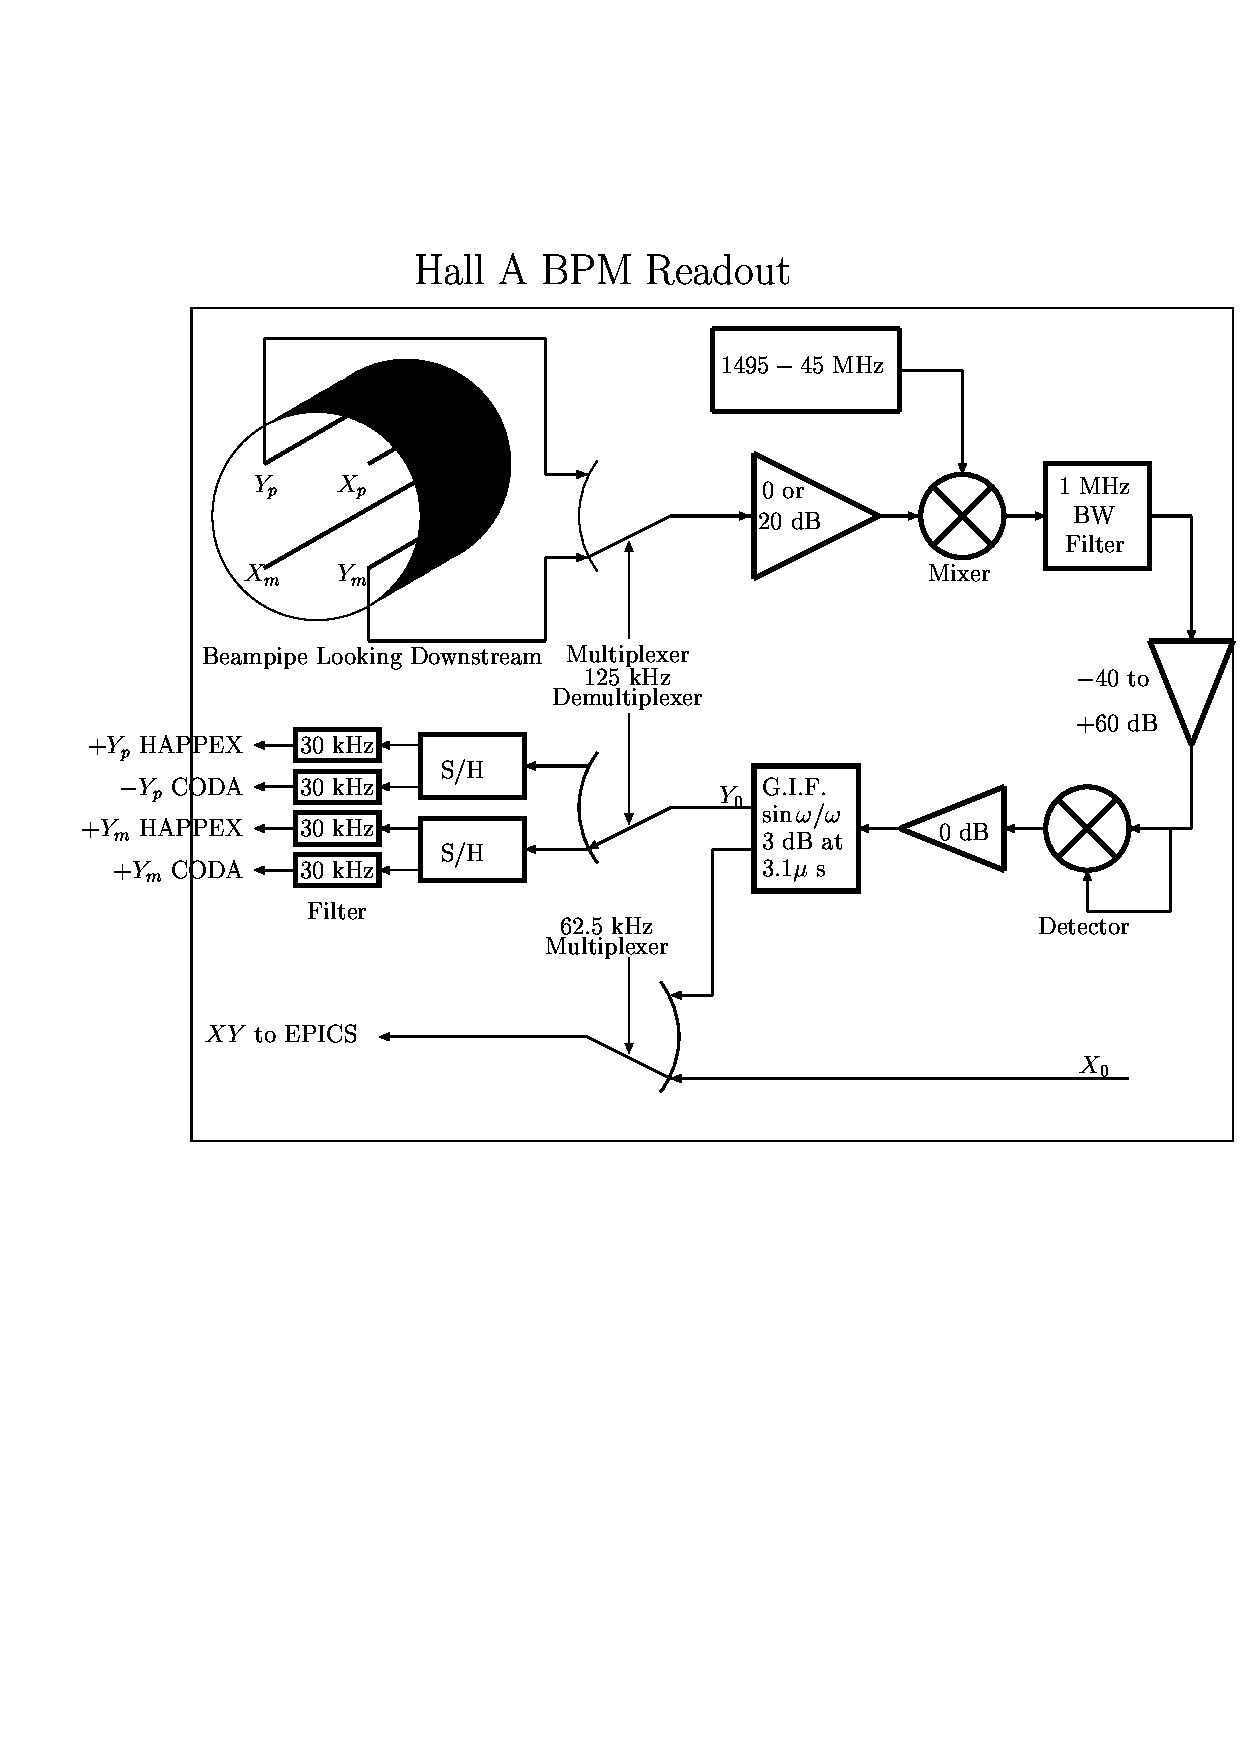
\includegraphics[angle=0,width=15cm]{BPM_fig}
{\linespread{1.}
\caption[Beamline: BPM Readout Electronics]{Schematic of the BPM readout
electronics}
\label{fig:bpmel}}
\end{center}
\end{figure}
}

1. The averaged position over 0.3 seconds is logged into the EPICS~\cite{EPICSwww} database (1 
Hz updating frequency) and injected into the datastream every 3-4 seconds, 
unsynchronized but with an orientative timestamp. From these values we can 
consider that we know the average position of the beam calculated in the EPICS 
coordinate system which is left handed.

2. Approximately once a shift (or more often if requested by the experimenters) 
a B-scope procedure ~\cite{bi:TP} can be performed using the same EPICS electronics 
which then gives the peak-to-peak variation of the beam.

3. Event-by-event information from the BPMs are recorded in the CODA datastream
from each of the 8 BPM antennas (2x4) from which the position of the beam can be 
reconstructed. However, these raw values belong to a parallel electronics chain 
whose constants have to be retrieved by calibrations to the EPICS or scanner 
data. 

\subsection{Beam Exit Channel}

After the target vacuum chamber, which was built by
the University of Virginia, there is an exit beam pipe which 
transfers the scattered beam onto the dump tunnel under vacuum. This exit beam 
pipe is made of a thin walled aluminum spiral corrugated pipe of welded 
construction. The largest diameter is 36 inches with a 0.164 inches wall 
thickness and the smallest diameter is 6 inches with a 0.042 inches wall 
thickness. The whole assembly is rather light (approximately 800 kg) and is 
supported by H shaped adjustable stands. To prevent possible linear collapse 
of the larger diameter sections under vacuum load, four aluminum channels of 
total cross-sectional area of 3'' are welded to its side. A vacuum of 
10$^{-5}$ Torr is maintained with a turbomolecular pump. The exit face of this 
pipe has a 12'' port and is connected to the diffuser with a Beryllium 
window.

}

\section{ Machine/Beamline protection system}
\label{sec:beam-fsd}

The MPS~\cite{MPScebaf} system is composed of the Fast Shutdown System (FSD), Beam Loss 
Monitor (BLM), and gun control system.

The FSD system is a network of permissive signals which terminate at the 
electron gun and chopper 1. The permissive to the gun and chopper
1 may be inhibited by any device connected to an FSD mode. Devices connected to the 
FSD system include vacuum valves, RF systems, Beam loss systems, beam current 
monitors, beam dumps, and particular to Hall A, the target motion mechanism 
and the raster (value and derivative).

The gun control system includes software program which monitors beam 
operating conditions and the state of the FSD and BLM systems. the program 
will warn the operators if a potential for beam damage exists. Potential for 
damage exists when running high average current beam, when FSD nodes are 
masked and when the beam power approaches the operating envelope limits for a 
specific beam dump.

\clearpage
\begin{safetyen}{10}{10}
\section{Safety Information}
\end{safetyen}
}
%
% Information for the ESAD
%

\begin{safetyen}{0}{0}

The beamline in the Hall provide the interface between the CEBAF accelerator
and the experimental hall.   All work on the beamline must be coordinated 
with both physics division and accelerator division; in order to ensure
safe and reliable transport of the electron beam to the dump.

\subsection{Hazards and Mitigations}

All magnets (dipoles, quadrupoles, sextupoles, beam correctors) and beam 
diagnostic devices (BPMs, scanners, Beam Loss Monitor, viewers) necessary for 
the transport of the beam are controlled by Machine Control Center (MCC) 
through EPICS~\cite{EPICSwww}, except for special elements which are addressed in the 
subsequent sections. The detailed safety operational procedures for the Hall 
A beamline should be essentially the same as the one for the CEBAF machine 
and beamline.\\ 

  
\noindent{}Personnel who need to work near or around the beamline should keep in mind the potential hazards:
\begin{itemize}
  \item Radiation ``Hot Spots'' - marked by ARM or RadCon personnel,
  \item Vacuum in the beam line tubes and other vessels,
  \item Thin windowed vacuum enclosers (e.g. the scattering chamber),
  \item Electric power hazards in vicinity of the magnets,
  \item Magnetic field hazards in vicinity of the magnets, and
  \item Conventional hazards (fall hazard, crane hazard etc.).
\end{itemize}

The most hazardous areas along the beamline are roped off it restrict access.   
In particule the scattering chamber, with it's large
volume and thin windows requires hearing protection once it has been evacuated.   
Signs are posted by radcon for any hot spots along the beamline and
radcon must be notified before work is done in a posted area.

Some magnets, as the M{\o}ller spectrometer elements, are covered with plastic
sheets for electric safety. Any access to these magnets requires
the ``Lock and Tag'' procedure~\cite{EHScebaf} and the appropriate training,
including the equipment-specific one. \\

\noindent{}Additional safety information is available in the following documents:
\begin{list}{--}{\setlength{\itemsep}{-0.15cm}}
  \item EH\&S Manual~\cite{EHScebaf};
  \item PSS Description Document~\cite{PSScebaf}
  \item Accelerator Operations Directive~\cite{AODcebaf};
\end{list}

\subsection{Responsible Personnel}

Since the beamline requires both accelerator and physics personnal to maintain
and operate and it is very important that both groups stay in contact that any 
work on the Hall A beamline is coordinated.

\begin{namestab}{tab:beam:personnel}{Beam line: authorized personnel}{%
   Beamline physics division and accelerator divison points-of-contact.}
  \namestabheader{Hall A Physicists}
  \DouglasHiginbotham{\em 1st Contact}
  \RobertMichaels{\em 2nd Contact}
  \namestabheader{Liaisons from Accelerator Division}
  \HariAreti{..to Physics}
  \YvesRoblin{..to Hall-A}
\end{namestab}
\end{safetyen}


\newpage
\section{ Beam Position Monitors}

To determine the position and the direction of the beam on the experimental 
target point, two Beam Position Monitors (BPMs) are located at distances 7.524 m 
(IPM1H03A) and 1.286 m (IPM1H03B) upstream of the target position. 
The BPMs consist of a 4-wire antenna array of open ended thin wire striplines 
tuned to the fundamental RF frequency of 1.497 GHz of the beam ~\cite{bi:bar90}. The 
standard difference-over-sum technique is then used ~\cite{bi:HW} to determine the 
relative position of the beam to within 100 microns for currents
above 1 $\mu $A. The absolute  position of the BPMs can be calibrated with respect to the 
scanners (superharps) which are located adjacent to each of the BPMs (IHA1H03A 
at 7.353 m and IHA1H03B at 1.122 m upstream of the target). The schematic of the 
readout electronics is shown in Figure ~\ref{fig:bpmel}. The
position information from the 
BPMs can be recorded in three different ways:

\begin{figure}
\begin{center}
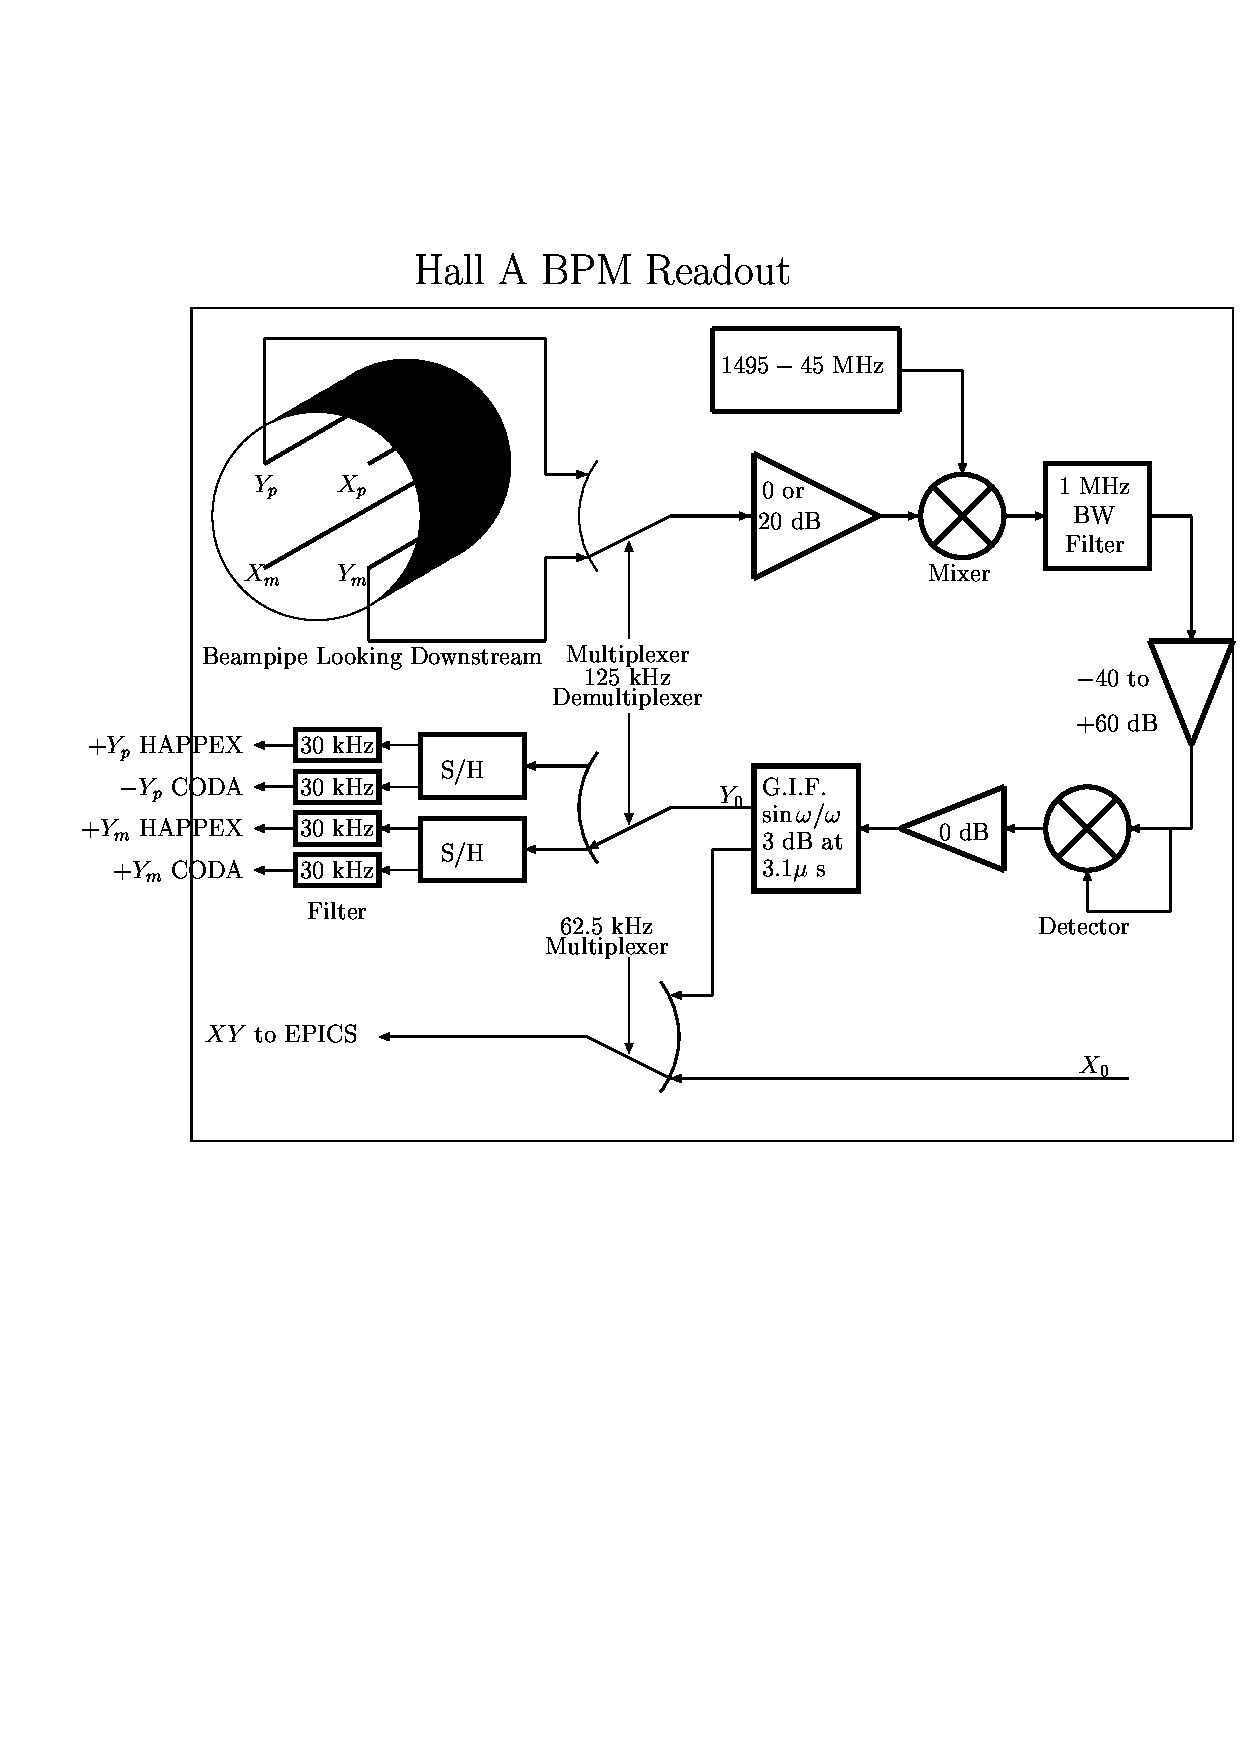
\includegraphics[angle=0,width=15cm]{BPM_fig}
{\linespread{1.}
\caption[Beamline: BPM Readout Electronics]{Schematic of the BPM readout
electronics}
\label{fig:bpmel}}
\end{center}
\end{figure}

\vskip 0.5cm

1. The averaged position over 0.3 seconds is logged into the EPICS database (1 
Hz updating frequency) and injected into the datastream every 3-4 seconds, 
unsynchronized but with an orientative timestamp. From these values we can 
consider that we know the average position of the beam calculated in the EPICS 
coordinate system which is left handed.

\vskip 0.5cm

2. Approximately once a shift (or more often if requested by the experimenters) 
a B-scope procedure ~\cite{bi:TP} can be performed using the same EPICS electronics 
which then gives the peak-to-peak variation of the beam.

\vskip 0.5cm

3. Event-by-event information from the BPMs are recorded in the CODA datastream
from each of the 8 BPM antennas (2x4) from which the position of the beam can be 
reconstructed. However, these raw values belong to a parallel electronics chain 
whose constants have to be retrieved by calibrations to the EPICS or scanner 
data. 


%\begin{thebibliography}{99}
%\bibitem{bi:bar90} W. Barry et al., CEBAF-PR-90-009 (1990).
%\bibitem{bi:HW} C. Hyde-Wright et al., Beam Position Studies for E93050 and priv. comm..
%\bibitem{bi:TP} T. Powers, priv.  comm.. 
%\end{thebibliography}
% ===========  CVS info
% $Header: /group/halla/analysis/cvs/tex/osp/src/beamline/bpms.tex,v 1.1 2003/06/05 17:28:32 gen Exp $
% $Id: bpms.tex,v 1.1 2003/06/05 17:28:32 gen Exp $
% $Author: gen $
% $Date: 2003/06/05 17:28:32 $
% $Name:  $
% $Locker:  $
% $Log: bpms.tex,v $
% Revision 1.1  2003/06/05 17:28:32  gen
% Initial revision
%

\newpage
\section[Beam Current Measurement]{Beam Current Measurement
\footnote{
  $CVS~revision~ $Id: bcm.tex,v 1.5 2003/12/13 06:23:37 gen Exp $ $
}
\footnote{Authors: A.Saha \email{saha@jlab.org}}
}

The Beam Current Monitor (BCM) is designed for stable, low noise, non-intercepting 
beam current measurements. It consists of an Unser monitor, two rf cavities, 
the electronics and a data acquisition system. The cavities and the Unser monitor 
are enclosed in a box to improve magnetic shielding and temperature stabilization.
The box is located 25 m upstream of the target. You can recognize it as a grey 
object on the stands, about 2 m downstream from where the beam enters the 
hall. 

The DC 200 down-converters and the Unser front end electronics are located in Hall 
A. The temperature controller, the Unser back end electronics and its calibration 
current source, cavity's RF unit (housing the RMS-to-DC converter board) and all 
multi-meters, VME crate and computers are located in Hall A control room.

\infolevone{
\subsection{ System Layout}

The schematic diagram of the BCM system is presented in
Fig.~\ref{fig:halla_bcm}.
\begin{figure}[htp]
\begin{center}
\includegraphics[angle=0,width=0.9\textwidth,clip]{habcm_r}
{\linespread{1.}
\caption[Beam Current Measurement: Schematic]{Schematic of the Hall A beam
current measurement system.}
\label{fig:halla_bcm}}
\end{center}
\end{figure}

The Unser monitor is a Parametric Current Transformer designed for non-destructive 
beam current measurement and providing an absolute reference. The monitor is 
calibrated by passing a known current through a wire inside the beam pipe and has a 
nominal output of 4 mV/$\mu $A. It requires extensive magnetic shielding and 
temperature stabilization to reduce noise and zero drift. As the Unser monitor's 
output signal drifts significantly on a time scale of several minutes, it cannot be 
used to continuously monitor the beam current. However, this drift is measured 
during the calibration runs (by taking a zero current reading) and removed in 
calibrating the cavities.  The more stable cavities are then used to determine the 
beam current and charge for each run. We also use the OLO2 Cavity Monitor and the 
Faraday Cup 2 at the Injector section to provide an absolute reference during 
calibration runs.

The two resonant rf cavity monitors on either side of the Unser Monitor are 
stainless steel cylindrical high Q ($\sim 3000$) waveguides which are tuned to the 
frequency of the beam (1.497 GHz) resulting in voltage levels at their   outputs 
which are proportional to the beam current. Each of the rf output signals from the 
two cavities are split into two parts. One part of the signal is  converted to 10 
kHz signals (by the ``downconverters'') and fed into an RMS-to-DC converter board 
consisting of a 50 kHz bandpass filter to  eliminate noise, amplified and split to 
two sets of outputs, which after further processing are recorded in the data 
stream. These two paths to the data stream (leading to the sampled and integrated
data ) will now be described. (The other part of the split signal is downconverted 
to 1 MHz signals and represents the old system (pre Jan 99). Only the HAPPEX 
collaboration presently uses these signals.)

For the sampled (or EPICS~\cite{EPICSwww} or Slow) data, one of the amplifier outputs is sent to a 
high precision digital AC voltmeter (HP 3458A). Each second this device provides 
a digital output which represents the  RMS average of the input signal during that 
second.  The resulting number is  proportional to the beam charge accumulated 
during the corresponding second (or, equivalently, the average  beam current  for 
that second). Signals from both cavity's multi-meters, as well as from the 
multi-meter connected to the Unser, are transported through GPIB ports to the HAC 
computer where they are recorded every 1 to 2 seconds via the data-logging process 
which is described in the calibration procedure. They are also sent through EPICS 
to CODA and the data stream where they are recorded at  quasi-regular intervals, 
typically every two to five  seconds.

For the integrated (or VTOF or Fast) data, the other amplifier output is sent to an 
RMS-to-DC converter which   produces  an analog DC  voltage  level. This level 
drives a Voltage-To-Frequency (VTOF) converter whose output frequency is  
proportional to the  input DC voltage level. These signals are then fed to Fastbus  
scalers and are finally injected into the data stream along  with the other scaler 
information.  These scalers simply accumulate during  the run, resulting  in a 
number which is proportional to the time integrated voltage level and therefore 
more accurately represents the true integral of the current and hence the total 
beam charge. The regular RMS to DC output is linear for currents
from about 5 $\mu$A to somewhere well above 200 $\mu$A.
 Since it is non-linear at the lower 
currents, we have introduced a set of amplifiers with differing gains (x3 and x10) 
allowing the non-linear region to be extended to lower currents at the expense of 
saturation at the very high currents. Hence there are 3 signals coming 
from each BCM (Upx1, Upx3, Upx10, Dnx1, Dnx3, Dnx10). All 6 signals are fed 
to scaler inputs of each spectrometer (E-arm and H-arm) . Hence we have a 
redundancy of 12 scaler outputs for determining the charge during a run. During 
calibration runs we calibrate each of these scaler outputs.   
}

\begin{safetyen}{10}{10}
\subsection{ Authorized Personnel}
\end{safetyen}

All Hall A members are authorized to take BCM calibration data using the Standard 
Non-Invasive Hall A BCM Calibration Procedure. The extended calibration procedures 
involving the Faraday Cup 2 and the OLO2 monitor at the Injector are presently 
performed by A. Saha. 

\vskip 0.2cm

The Accelerator AES group performs the maintenance of the BCM monitors. These 
include:

\begin{tabular}{l l}
1. The Unser calibration. & Every 3 months \\
2. Resonant Cavities Tuning. & Every Downtime \\
3. Multi-meters Autocalibration. & Every Downtime \\
4. Connectors Cleaning. &  Every year \\
5. Unser Keithley Current Source. & Calibration Yearly \\
6. Digital Multi-meters HP3458A and HP 34401A. & Calibration Yearly\\   
\end{tabular}

System Contacts are shown in Table~\ref{tab:BCM:personnel}.
\begin{namestab}{tab:BCM:personnel}{BCM: authorized personnel}{%
   Beam Current Monitor: authorized personnel}
  \ArunSaha{\em Contact}
  \JohnMusson{Accel. expert}
\end{namestab}
%Jean-Claude Denard -x 7555




% ===========  CVS info
% $Header: /group/halla/analysis/cvs/tex/osp/src/beamline/bcm.tex,v 1.5 2003/12/13 06:23:37 gen Exp $
% $Id: bcm.tex,v 1.5 2003/12/13 06:23:37 gen Exp $
% $Author: gen $
% $Date: 2003/12/13 06:23:37 $
% $Name:  $
% $Locker:  $
% $Log: bcm.tex,v $
% Revision 1.5  2003/12/13 06:23:37  gen
% Septum added. Name tables. Polishing
%
% Revision 1.4  2003/12/05 05:48:30  gen
% Polishing
%
% Revision 1.3  2003/06/06 15:19:02  gen
% Revision printout changed
%
% Revision 1.2  2003/06/05 23:29:59  gen
% Revision ID is printed in TeX
%
% Revision 1.1.1.1  2003/06/05 17:28:32  gen
% Imported from /home/gen/tex/OSP
%
%  Revision parameters to appear on the output

\newpage
\section[Fast Raster]{Fast Raster
\footnote{Authors: R.~Michaels \email{rom@jlab.org}}
}


The beam is rastered on target with an amplitude of
several millimeters at 25 kHz to prevent overheating.  
The raster is a set of four of air-core dipoles located
approximately 23 m upstream of the target. 
Two dipoles are for horizontal (X) motion and
another two for vertical (Y).  During the 6 GeV era
there was only one pair of X and Y, but we have doubled
the raster to account for the energy increase to 11 GeV.
The arrangement along the beamline along the 
direction of the beam will be XXYY.

For a typical 40A current in the raster coils, the
deflection by one pair (e.g. the X direction) of coils, 
in radians, is $\theta = 1.94 \times 10^{-3}/ E$
where $E$ is the electron's energy in GeV.
For example, at $E = 6$ GeV, a 0.32 mrad deflection is achieved.
Projected onto the target (about 21 m away) this is a $\pm$ 6.8 mm
excursion {\it if} there were no other magnetic fields 
between the raster and the target; however, there are quadrupoles
which change this depending on the beam tune.

Since 2003 we've used the triangle-wave 
raster pattern designed by Chen Yan.  
This achieves a very uniform rectangular
density distribution of beam on the target 
by moving the beam with a time-varying dipole
magnetic field whose waveform is triangular
with very little dwell time at the peaks.  
The electronics design is an ``H-bridge''
in which switches are opened and closed 
at 25 kHz, to switch between two directions 
of current (100 A peak-to-peak) 
through the raster coils.

Three new features during the 12-GeV era are 
1) the driver of the H-bridge electronics is now
an Agilent model 33522A waveform generator; and
2) The two X are synchronized with each other, and
the two Y are synchronized.  This makes the kicks
add and allows us to accomodate the higher energy
of the beam; and 3) The entire raster can
be synchronized to an external 10 MHz wavetrain
supplied by the polarized injector electronics.
This makes the nominal 25 kHz an exact multiple of
the helicity-flip rate, which achieves a cancellation
of raster noise, important for parity-violation 
experiments only.
The syncrhronization of the pairs of X and Y are
accurate to within a few nsec.

For most users, these three new features will not be
noticeable and the raster will appear to function
the same as during the 6 GeV running.
A user can view the 
status of the raster in the
EPICS overview screen called ``General Accelerator
Parameters'' where the set-point for the radius amplitude
and the readback of the peak-current in the raster are displayed.

Control of the raster is done by first asking the MCC
operators to set up the raster for a particular size
typically 2 mm square.
The control software assumes a field-free region between
the raster and the target, so it is only approximately
correct because there are several quadrupoles in this region.
It is important to check the raster spot size and
make adjustments if necessary.  The adjustment is made
by asking MCC to change the size and noting the 
linear relationship between what their software says
the size is and the actual size.
Relatively small independent adjustments to the 
gains on the X and the Y raster
coils are available in the middle room of the hall A
counting room using the ``PGA Controller'' knobs;
however, it is not recommended to touch these.
Near these knobs is also located an oscilloscope X-Y trace
of the current in the raster.  A fast shutdown (FSD) shuts
the beam down within 0.1 msec if the raster fails, thus
affording some protection of the target.

{\it NOTE:  If you are unsure of the status of the raster,
measure the spot size with very low current ($\le 2 \mu$A) or with
the target out of the beam.}  It would be a mistake
to check the beam spot size with high current on target; by
the time you check it, the target may already be destroyed.
The rastered beam spot on target can be checked with
plots in the ROOT analyzer or by 
using the stand alone code called \mycomp{spot},
also called \mycomp{raster}.
For more details on usage, type \mycomp{spot -h} (help)
on the ADAQ computers.

Regarding the BPM measurements, it should be noted that 
the stripline BPMs displayed by \mycomp{spot} have a high-frequency 
cutoff of approximately 30 kHz.  Since the raster frequency is 25 kHz
the plot of the amplitude distribution shows spikes at the 
limits of the orbit, instead of a flat distribution.  The scale
factor between what is seen in \mycomp{spot} and the real width of the beam
is $\sim 1.5$, i.e. the beam is 1.5 times bigger than the naive
reading of the \mycomp{spot} distribution.



\newpage
% Updated Comments Dec. 2
\infolevone{
\chapter[Arc Energy Measurement]{Arc Energy Measurement
\footnote{Authors: D. Higinbotham \email{doug@jlab.org}}
}
}

\infoleveqnull{
\section{Arc Energy Measurement}
\subsection{Overview}
In order to determine the integral field of the eight dipoles that lead to Hall A, and 
in turn determine the beam energy, a nineth dipole wired in series with the rest is 
located in a special shed near the hall A counting house.
}

\infolevone{
The ARC energy measurement is under EPICS~\cite{EPICSwww} control through 
a MEDM~\cite{MEDMwww} display. Two
independent control systems are used: the beam bend angle measurement through
the arc ("scanners") and the field integral of
the arc ("integral"). To measure the energy: 

\begin{itemize}
\item perform several angle measurements 
\item perform an integral measurement 
\item analyze the integral measurement and note the value of the arc field 
integral 
\item analyze the angle measurements, average the results (proposed by the 
software),
then ask for the energy calculation, enter the above arc field integral and
you will get the beam energy computed from the average angle. 
\end{itemize}

\section{Summary of ARC operations }

Six scanners of the same type, called ``ARC scanner'' and labelled
from scanner \#1 to \#6, are installed on the Hall-A beamline. Scanners \#1
to \#4 are used for the ARC energy measurement and they are located on the Hall-A
arc: \#1 [1HA1C07A] and \#2 [1HA1C07B] just upstream of the arc, in the BSY, and 
\#3 
[1HA1C18A] and \#4 [1HA1C18B] in the Hall-A
tunnel, just upstream the Compton polarimeter. Scanners \#5 [1HA1H03A] and \#6 
[1HA1H03B] 
are located
between the Moller and the target to control the beam geometry on the target
and their use will not be discussed here. 

Procedure for running a harp scan is described elsewhere\footnote{
Harp scan procedure \url{http://hallaweb.jlab.org/equipment/beam/harp_halla/harp.html}.}

Each scanner has a motor/ball-screw/shaft-encoder/vacuum-penetrator system moving
accurately a set of 3 tungsten wires through the beam. Each time a wire crosses
the beam a PMT located a few meters downstream records a signal due to the 
electromagnetic
shower induced by the beam in the wire. Both forward and backward passes are
recorded. The motion is a horizontal translation and, for a forward pass: 

-the translation is from beam left to beam right, 

-the two first wire crossing the beam are at 45deg from the vertical, 

-the third wire, which is the only important for the ARC energy measurement,
is vertical. 

Recording, during the scan, the scanner position and the PMT output voltage
allows us to determine the beam position at each scanner location. Then, using
calibration data not detailed here, we deduce the net beam bend angle through
the arc. This result measured in dispersive arc tuning, along with the field
integral of the arc dipoles, provides an accurate determination of the beam
energy. 

\vspace{0.3cm}

\section{Summary of field integral }

The purpose is to measure absolutely the straight field integral of a 
"BA"
3m long dipole, called the "9th dipole" and located in the
"Dipole Shed". It is of the same type as the 8 arc dipoles
and is powered in series with them. 

The ARC integral setup is basically made of a 3m long plate (the 
"probe")
which is able to move inside the 9th dipole gap along the beam axis and carrying 
two
field measurement devices: a pair of pick-up coils connected in series and a
set of NMR probes. The coils are on both ends of the probe and the NMRs close
to the center. 

-at the "upstream" probe position, the 
"downstream"
coil is close to the dipole center, the "upstream" is outside
the dipole and the NMRs at one end of the dipole: 

Door$<-$-- ....................$<-$-------DIPOLE-----$--->$ 

.............$<-$-------PROBE------$--->$ 

-at the "central" probe position, each coil is at one end
of the 3m long dipole and the NMRs close to the dipole center: 

Door$<-$-- ...................$<-$-------DIPOLE-----$--->$ 

..................................$<-$-------PROBE------$--->$ 

-at the "downstream" probe position, the 
"upstream"
coil is close to the dipole center, the "downstream" is outside
the dipole and the NMRs at one end of the dipole: 

Door$<-$-- ...................$<-$-------DIPOLE-----$--->$ 

....................................................$<-$-------PROBE------$--->$ 

We call upstream the position where the probe is the closest to the shed access
door. Among the 3 above positions, the only one where the NMR can lock on the 
dipole
field is the central one as in the extreme position of the probe, the field 
homogeneity
is not sufficient. The probe position is controlled by a linear encoder. The
Z axis refers to the "beam" direction, increasing from upstream
to downstream. We use three kinds of "Z": 

-Zm to locate a point inside the magnet. The dipole center is at Zm=0 and the
yoke ends at +-1500.mm 

-Zp to locate a point inside the probe. The probe center is at Zp=0. Each of
the 4 NMR probes has a Zp given in the file "magnet.dir".
At a temperature of 21C, the coils are at Zp=+-1519.815mm (from magnet.dir) 

-Zd to refer to a displacement of the probe w.r.t. the dipole. Zd=0 refers to
the upstream (home) position of the probe. The integral measurement is performed
from Zd=0.000mm (1st PDI trigger) to Zd=3199.000mm (last PDI trigger), for forward
pass. Zd is given by the display (at the top of the rack) or by the master screen
("OUT"). 

The relationship between Zm, Zp and Zd is: 

Zd-Zm+Zp=C 

where C is a constant given in magnet.dir (C=1604.000 nomin.). Example of use:
to have the probe center at the dipole center, one must set Zd=1604.000mm (set
Zm=0 and Zp=0 in the above formula, and solve for Zd) 

The integral measurement sequence is the following: 

-from the current position (a priori arbitrary) move the probe upstream, up
to a limit (optic) switch. 

-move downstream by a few mm to cross the encoder index (encoder initialization) 

-move to the central position to measure the central field by NMR, the system
checks if the NMR locks and if the reading is stable, it will be the 
"before"
field 

-move back to upstream position 

-move to downstream position while integrating the flux through the coil system,
this measurement will be called the "forward" integral (duration
\( \sim  \) 7s) 

-move back to upstream position while integrating the flux through the coil
system, this measurement will be called the "backward" integral
(duration \( \sim  \)7s) 

-move to the central position to measure the central field by NMR, the system
checks if the NMR locks and if the reading is stable, it will be the 
"after"
field. 

In addition to the central field, 4 probe temperatures, a local excitation current
measurement, the setting of the dipoles P.S, the readback of the dipoles P.S
and the probe position at NMR measurement time are recorded 
"before"
and "after". 

To perform an integral field measurement: 

1-check if the system works (see "details on integral system 
check"
below) 

2-run the above integral sequence (see "details on integral run"
below) 

3-fix the error(s) if any (see "details on integral errors"
below) 

4-save the data in a file (see "details on integral data save"
below) 

5-analyze the data  


\section{Details on integral run }

To run the integral measurement sequence, call the 
\mycomp{arc\_integral.adl}
medm screen, then: 

-push "start" to start the full sequence 

-look at the results displayed: 

-after the "before" NMR measurement: the 
"before"
data set 

-after the "forward" integral pass: the forward velocity profile
and the forward voltage-after-gain profile 

-after the "backward" integral pass: the backward velocity
profile and the backward voltage-after-gain profile 

-after the "after" NMR measurement: the 
"after"
data set 

-if "BAD NMR" or "PDI saturation" flags
are set, or if something is obviously wrong in the data or plots, call expert. 

-data are ready to be saved (see "Details on integral data save"
below) 


\section{Details on temperatures }

The AC system of the shed is made of two cooling units, a heating unit and a
controller connected to two temperature sensors : one located in the shed and
one located in the BSY. This system is programmed in such a way that the 
temperature
of the shed follows the BSY temperature within +-2C. The BSY temperature can
be anywhere in the 18C to 35C range, regardless of the season. The BSY 
temperature
and the shed temperature are given (in F) by a display panel located close to
the workstation, on the wall. The AC system can be set in manual control by
turning from "auto" to "manual" a set of
switches controlling the cooling units and the heater unit. These switch boxes
are located on the shed wall. If the shed temperature is above 34.4C (94F),
call the crew chief (the electronics can be damaged) and cool down the shed in manual
AC mode. The 4 temperature sensors of the probe are labelled Tx+z+, Tx+z-, Tx-z+,
Tx-z- depending on their position w.r.t. the frame. 

Both "x+" sensors are on the probe edge which is inside the
dipole gap and both "x-" sensors on the opposite edge which
is outside the dipole gap. Both "z-" sensors are at 1/4 of
the long dimension of the probe and both z+ at 3/4 of this length. The average
of the 4 temperatures is used by the analysis program to correct the coil distance
from the thermal expansion of the probe, so it is important to make sure that
the 4 sensors are working well. The user can just make sure that the temperatures
displayed in \mycomp{arc-master.adl} or recorded in 
\mycomp{arc-integral.adl}
are realistic. In \mycomp{arc-integral.adl} they are given in the
order: Tx+z-, Tx+z+, Tx-z-, Tx-z+ Tx-z- and Tx-z+ should be close to the shed
temperature. Tx+z- and Tx+z+ depend on the probe position, as the gap (iron
yoke) is warmer than the shed and the dipole coil (at both ends of the dipole)
is warmer than the iron yoke. For a probe in a central position for more than
about one hour, the Tx+z- and Tx+z+ sensors should give the yoke temperature,
i.e the shed temperature plus 0. to 5.C, depending on the current, LCW temperature
and the magnet/shed temperature history. The 4 temperatures are also displayed
inside the shed, on the electronics rack. These values are digitized by separate
ADCs, so they may differ from the remote values by \( \sim  \)0.1C. 
}

\begin{safetyen}{10}{10}
\infolevone{\section{Shed access and safety }}

Due to the the dipole magnet and motion system, the access to the shed is limited to authorized
persons which are listed in the ESAD and listed below. To be added to the list, 
contact Douglas Higinbotham.
The standard
operation mode of the integral measurement setup is the remote mode, through
the network, from the counting house.
\end{safetyen}

\begin{safetyen}{10}{10}
\infolevone{\section{List of Authorized Personnel for Shed Access}}
\infoleveqnull{\subsection{List of Authorized Personnel for Shed Access}}
\end{safetyen}
\begin{namestab}{tab:arc:personnel}{Arc Energy Measurement: authorized personnel}{%
                 Arc Energy Measurement: authorized personnel}
  \namestabheader{Hall A Personnel}
  \DouglasHiginbotham{\em Contact}
  \namestabheader{Accelerator Personnel}
  \MichaelTiefenback{}
  \YvesRoblin{}
  \RickGonzales{}
  \BillMerz{}
  \MarkAugustine{}
  \HariAreti{}
  \PeteFrancis{}
  \ScottHiggins{}
  \DavidSeidman{}
  \RonLauze{}
  \TonyDay{}
  \ChristopherCurtis{Alignment group}
  \namestabheader{CEA - Saclay experts}
  \PascalVernin{}
  \ChristianVeyssiere{}
  \FrancoisGougnaud{}
  \JacquesMarroncle{}
\end{namestab}



\newpage
\infolevone{
\chapter[Target Chamber]{Target Chamber
\label{sec:target_chamb}
\footnote{
  $CVS~revision~ $Id: tgtcham.tex,v 1.11 2005/04/04 22:27:25 gen Exp $ $
}
\footnote{Authors: ?? \email{??@jlab.org}}
}

The cryo-targets and the waterfall targets 
(see Sec.~\ref{sec:targets-overv}) 
are contained in a special target chamber which is a large 
evacuated  multistaged can. So far, three chambers have been designed:
\begin{list}{\arabic{enumi}.~}{\usecounter{enumi}\setlength{\itemsep}{-0.15cm}}
  \item a chamber used up to 2003;
  \item a chamber designed for use with septum magnets, starting in 2003;
  \item a chamber designed for use with the BigBite spectrometer.
%\footnote{
%        No yet manufactured by Dec,2003.}.
\end{list}

Here, chamber 1 is described. Chambers 2 and 3 are only different in 
size and slightly in shape. The safety considerations fully apply to chambers 2 and 3.
The chamber was designed to isolate the beam line vacuum from  each
HRS so that each HRS could rotate
around the target without vacuum coupling and without jeopardizing
certain desired kinematic and acceptance  specifications of 
both high resolution spectrometers
needed for approved experiments.  It  was also designed to simultaneously
 contain a liquid or gas target and an array of water cooled thin
 metallic foils, both remotely controlled and also be adaptable for
the waterfall target. The desired kinematic specifications that were
 considered included momentum and energy resolution in both arms,
 angular range of spectrometers, angular acceptance, and luminosity.
The chamber vacuum is isolated from the  HRS by using thin aluminum foils. 

The target chamber is designed so that
each spectrometer will have continuous coverage in the standard tune from
$\theta_{min}=$12.54$^\circ$ to $\theta_{max}=$165$^\circ$.
The aluminum window is 6~$in$ high and 0.016~$in$ thick made of 5052 H34 aluminum foil.
The foil forms regularly spaced vertical ridges when
placed under load. The window had an inter-ridge
spacing of 3 inches.
If the window is treated as a collection
of smaller rectangular windows which have the full vertical height
of 6 inches and the inter-ridge spacing as a width,
then stress formulas predict that the 0.016 $in$
material would reach ultimate stress at a pressure higher than 35 PSID
(for both over-pressure and under-pressure). 
There is a gate valve between the 
scattering chamber and the beam entrance (exit) 
pipe. Both 
valves will be closed automatically in the
event that the chamber vacuum begins to rise and an FSD will be caused
( this is done via a relay output of the scattering
chamber vacuum gauge). If either valve is closed an FSD will result.

The target chamber is supported by a 24 $in$ diameter pivot post
secured in concrete, rising about 93.6 $in$ above the Hall A cement floor.
The Hall A target chamber
consists of an aluminum middle ring, a stainless steel base ring,
each with a 41.0 $in$ inner diameter,
and a stainless steel cylindrical top hat with 40 $in$ inner diameter
to enclose the cryotarget and secure the cryogenic connections.

When the scattering chamber is under vacuum, there is a potential
danger of window rupture.
The loud noise from the rupture could hurt
one's ears if not protected. Therefore when the chamber is under vacuum,
protective covers are put on if possible. These must be taken off
for data taking. For restricted access, the protective cover is required
to be on when the chamber is under vacuum. Before switching from controlled
access to restricted access, the protective cover is required to be installed.
Anytime that the scattering chamber
is under vacuum, the pivot area is enclosed in a rope or tape barrier
and a warning sign is posted.
Hearing protection is required in the enclosed area.

\infolevone{
	The aluminum ring with an outer diameter of 45.0 $in$ and
wall thickness 2.0 $in$  is necessary for a sturdy support structure and
to permit machining of the outside surface to accommodate
the flanges for fixed and sliding seals mounted on
opposite sides of the ring that vacuum connect the chamber to each HRS.
The height of the aluminum ring shown is 36.0 $in$, which is
designed to accommodate the mounting flanges.
The stainless steel base ring 
is 11.50 $in$ in height with
one pump-out 6 $in$ diameter port  and with
seven 4 $in$ viewing and electrical feed-through ports.
The base ring will also contain support mechanisms for the solid
target ladder assembly, a rotisserie for collimating slits, radiators, and
magnetic
fingers for
removing the solid target vacuum-lock can. The total height of the top
ring, middle ring, and
base ring is 93.81 $in$. This length is partly determined by our desire to
include with the cryogenic extended target a solid target vertical ladder
secured in an inverted hat through a hole in the base of the chamber.

	The base ring includes an end plate through which the
inverted hat will be adapted to fit into the large vertical pipe serving
as the pivot post for the Hall A spectrometers.

	The stainless steel cylindrical top hat  has
40.0 $in$ inner diameter, and is 0.375 $in$ thick and
46.31 $in$ high , which is necessary to permit the
cryotarget to be withdrawn and to make space available to expose the solid
targets to the electron beam.

   The 200 $\mu$A electron beam, focused to a $\sim$\(0.1\, mm\times
0.1\) mm spot and rastered $\pm$5 mm horizontally or vertically on the
target, enters through a oval hole in the middle ring which
is 2.06 $in$ wide and exits through a 1.81 $in$ hole connected to the
exit pipe.
}

\infolevone{
\section{Target Chamber - Spectrometer Coupling}

   The aluminum middle ring will support a flange on each side for each high
resolution spectrometer. Four flanges will be available: Two flanges will
contain a 6 $in$ window opening which will be covered with a thin foil
(e.g., 10 mil aluminum) .
These two flanges will be used for experiments utilizing
extended  targets that do not require optimum momentum resolution.
The other two flanges will have two fixed ports (with a 8 $in$ $\times$ 6 $in$
opening)
which will be mainly used for calibration of the spectrometers . Fixed ports are
centered at 16.11 $^\circ$ and
45 $^\circ$ for one flange and at 16.11 $^\circ$ and 90 $^\circ$ for the second
flange.

   For a point beam on target a vertical opening in the walls of the chamber
of height 57.15 cm x 0.065 x 2 = 7.43 cm is required so that the scattered
beam is within the full acceptance of the spectrometer.
If the beam is rastered on target $\pm$0.5 cm in the vertical direction,
then the opening in the outer side of the chamber must be at least 8.5 cm for
full acceptance.

From consideration of the angular range of the spectrometers in the standard
tune, the scattered beam acceptance envelope, the effects of an
extended gas target on acceptance,
and the effects of a rastered beam $\pm$ 5 mm on acceptance,
the target chamber requires a window of at least 8.5 cm
high in the aluminum ring extending from 6.33 $^\circ$ (2.48 in) from the
beam exit point to 8.83 $^\circ$ (3.47 in) from the beam entrance point on one
side and a similar window on the other side of the beam.
For future considerations (e.g., using a third arm or sliding seal) the
width of the window on the middle ring was actually constructed
to be 17.78 cm (7 $in$).

\section{Stress Analysis of the Middle Ring}

Since the middle ring has an extensive cut across the midplane on both sides as
well as
entrance and exit holes and loaded with about 25,000 lbs, calculations of the
stresses
 and deformation of  the
midplane support area of the middle ring and deflection of the window opening
were made using the finite element analysis code ANSYS . The work was conducted
by a graduate student in the Department of Civil Engineering at the
University of
Virginia and a REU student.  A scaled down model of the middle ring was
constructed and then tested by applying forces to it using the Materials Testing
Service of the Department of Transportation at the University. ANSYS was first
checked by comparing calculations of the test model deflections to the actual
data. Agreement was  within $\pm$10\%. Results of ANSYS for the target
chamber showed that the maximum deflection of the opening of the window in the
middle ring varied from 0.007 $in$ to 0.015 $in$ depending on how the
middle ring
was loaded. This was decided to be a safe limit. In the final design, several
movable
7 $in$ long, 2 $in$ diameter aluminum support rods are placed in the
window for added support. In addition, flanges defining the ports and
coupling to
the spectrometers can be added, giving additional support to the middle ring.
Compressional stresses, calculated using ANSYS assuming the middle ring was
attached to the
top hat and loaded with 25,000 lbs, were less than 3000 psi 
almost everywhere.
However, stresses over small areas rose to levels 6000 psi near the entrance
and exit holes. These calculations indicated that we did not exceed the safety
limit of 15,000 psi for aluminum. A simple model calculation shown in Appendix
A  gives the result 1434 psi, which represents some average value over the
midplane
contact area.

\section{Vacuum Pumping System}

The vacuum in the target chamber is maintained by an Alcatel ( 880 l/s)
 turbomolecular vacuum pump. The pump is connected to a 6 $in$ port in the
stainless steel ring between 130
 $^\circ \le \theta_p \le 180 ^\circ$. The vacuum pump is
fastened to a horizontal pipe connected to the chamber. The vacuum pressure in
the chamber is about $10^{-5}$ mm. An additional Alcatel pump connected
to an 8 $in$ port should be added to obtain lower vacuum. Both
pumps may be isolated
from the target chamber using gate valves which are remotely operated
from the vacuum control rack and interlocked to the FSD system.


A 2 $in$ all metal gate valve is located between the entrance flange to the
chamber and the beam profile monitor.   
 An additional gate valve is located 2 m downstream of the
 target chamber to isolate the chamber from the exit beam pipe.
}
\begin{safetyen}{10}{15}
\section{Safety Assessment}
\end{safetyen}

The scattering chamber is typically a low maintenance item but it is a vacuum
system and hence problems may occur. The day to day operations of the cryogenic
targets are managed by the Hall A Staff while major maintenance operations are
handled by the Cryogenic Target Group (Physics Division). Occasionally the
cryogenic targets experience difficulties due to failures of the End Station
Refrigerator which supplies the coolant. In these cases the Cryogenics Group
of the Accelerator Division should be contacted.

\noindent{}The target chamber may pose several hazards:

\begin{list}{\arabic{enumi}.~}{\usecounter{enumi}\setlength{\itemsep}{-0.15cm}}
  \item {\bf Rupture of vacuum windows}. This hazard is mitigated by
        lexan guards on the vacuum windows, installed by the hall technicians
        either at the beginning of a ``restricted access'' period 
        %(see Sec.\ref{sec:Access}),
        or during ``control access'', in case an access to the target chamber area is needed.
        Installation and removal of the guards is included in the technician's checklists.
        When the chamber is under vacuum, it is mandatory to use ear protection in the chamber
        vicinity. The appropriate signs must be installed by the technicians. 

  \item {\bf Induced radioactivity}. The RADCON surveyor measures the level of induced
        radiation as a part of the general survey and may declare the target area 
        as ``High Radiation Area'', installing a rope protection around\cite{RWIcebaf}. 

\end{list}

Some other safety issues are discussed in the cryo-target chapter 
(see Sec.~\ref{sec:target-cryo-safety}).
%and also in the polarized target chapter (see Sec.~\ref{sec:target-he3-general}).

\begin{safetyen}{10}{15}
\section[Authorized  Personnel]{Authorized  Personnel}
\end{safetyen}

\begin{namestab}{tab:targ_chamb:personnel}{Target chamber: authorized personnel}{%
      Target chamber: authorized personnel. ``W.B.'' stands for the white board 
      in the counting house.}
  \TechonCall{\em Contact}
  \JessieButler{}
  \DaveMeekins{Target group}
  \JianPingChen{}
\end{namestab}
}

\newpage
\infolevone{\chapter[M{\o}ller Polarimeter]{M{\o}ller Polarimeter}
\setcounter{subsection}{0}}
\infoleveqnull{\section[M{\o}ller Polarimeter]{M{\o}ller Polarimeter}}

The Hall A beam line is equipped with a M{\o}ller 
polarimeter
whose purpose is 
to measure the polarization of the electron beam delivered to the hall. 

\begin{safetyen}{0}{0}

The M{\o}ller Polarimeter system has under gone a major upgrade and an Operational Safety Proceedure (OSP)
is being written and must be reviewed before its use.

\subsection{Hazards and Mitigations}

The hazards and mitigations for this system can be found in the OSP at the end of this document. 

%\infolevone{
%Safety checklist item for this device, located at the end of the beamline section, is solely to ensure
%the beam can be tranported safetly past this system prior to it's recommisioning.
%}

\subsection{Responsible Personnel}
\label{sec:moller-pers}

This list of system experts provided in case there is any question as to the status of system.

\begin{table}[h]
\begin{center}
\begin{tabular}{|ll|l|l|l|l|r|} \hline
  \multicolumn{2}{|c|}{Name} & Dept. & \multicolumn{2}{c|}{Telephone} & 
  \multicolumn{1}{c|}{e-mail} & Comment \\ 
  \cline{4-5}
   &  &   & JLab & Pager &  & \\ 
\hline
 Javier       & Gomez           & JLab    & 7498 & 7498 & gomez@jlab.org    & Primary contact     \\ 
 Oleksandr    & Glamazdin       & Kharkov & 5441 & 5441 & glamazdi@jlab.org &  \\ 
 Viktor       & Gorbenko        & Kharkov & 5441 &   -  & gorbenko@jlab.org &  \\ 
 Roman        & Pomatsalyuk     & Kharkov & 5395 & 0001 & romanip@jlab.org  &  \\ 
\hline
\end{tabular}
\end{center}
\caption[Moller Polarimeter: authorized personnel]{
   The listed name are those who are considered system experts of the Moller Polarimeter and should be contacted
   if there is any question as to the status of the system.
}
\label{tab:moller:personnel}
\end{table}
\end{safetyen}


\newpage
}
% Compton Polarimeter
\infolevone{\chapter[Compton Polarimeter]{Compton Polarimeter}
\label{sec:compton}
\footnote{Author: S.Nanda \email{nanda@jlab.org}}
}
\infoleveqnull{\section{Compton Polarimeter}
\subsection{Overview}}


The Hall A Compton polarimeter has undergone a major upgrade and an
new operational safety proceedure (OSP) is being written and reviewed before the
Compton can be used.   The hazards and mitigations for this system can be found in 
this OSP.

\subsection{Responsible Personnel}

\begin{namestab}{tab:compton:personnel}{Compton Polarimeter: authorized personnel}{%
          Compton Polarimeter: authorized personnel}
 \SirishNanda{Primary Contact}
 \JackSegal{Secondary Contact}
\end{namestab}

\infolevone{
\subsection{Authorized Personnel}

The list
of the presently authorized personnel is given in Table~\ref{tab:compton:personnel}.
Other individuals must notify and receive permission from
the contact person (see Table~\ref{tab:compton:personnel}) to get their names
add to list.

\begin{namestab}{tab:compton:personnel}{Compton Polarimeter: authorized personnel}{%
          Compton Polarimeter: authorized personnel}
 \SirishNanda{\it Contact}
 \JackSegal{Technical}
 \JosephZhang{Optics}
 \MartialAuthier{Engineering}
 \NathalieColombel{Mechanical}
 \PascaleDeck{Electronics}
 \AlainDelbart{Optics}
 \DavidLhuillier{Analysis}
 \YvesLussignol{EPICS}
 \DamienNeyret{DAQ}
 \GerardTarte{Electronics}
 \ChristianVeyssiere{Electronics}
\end{namestab}
}



%
% Old Material
%
% \chapter[eP Beam Energy Measurement]{eP Beam Energy Measurement
\footnote{
  $CVS~revision~ $Id: ep.tex,v 1.6 2003/12/13 06:23:37 gen Exp $ $
}
\footnote{Authors: B.Reitz \email{reitz@jlab.org}}
}
\label{sec:ep}
\section {Purpose and Layout}
\label{sec:ep_purpose}

The Hall A eP system is a stand-alone device to measure the 
energy of the electron beam. It is located along the beamline
17~m upstream of the target. The beam energy $E$ is determined by measuring
the scattered electron angle $\Theta_e$ and the recoil proton angle
$\Theta_p$ in the $^1$H$(e,e'p)$ elastic reaction according to the kinematic
formula:
\begin{equation}
E = M_p \frac{\cos(\Theta_e) + \sin(\Theta_e)/\tan(\Theta_p) - 1}{1 - \cos(\Theta_p)} + O(m_e^2/E^2),
\end{equation}
in which $M_p$ denotes the mass of the proton and $m_e$ the mass of the electron.
The schematic diagram of the eP system is presented in Fig. \ref{fig:ep_layout}. 
Two identical arms, each consisting of an electron and a corresponding proton 
detector system, made up of a set of 2~x~8 silicon micro-strip detectors in the
reaction plane, are placed symmetrically with respect to the beam along the 
vertical plane. The target consists of a rotating CH$_2$ tape.
Simultaneous measurements of the beam energy with both arms result
in cancellation, to first order, of uncertainties in the knowledge of the position
and direction of the beam. 
 \begin{figure}[htb]
    \begin{center}
        \includegraphics*[angle=0,width=0.9\textwidth]{ep_layout}
    \end{center}
    \caption[eP: Layout]{
            Schematic layout of the eP energy measurement system,
            showing the arrangement of its components, the polyethylene (CH$_2$) 
            target, the Cherenkov detectors, the silicon micro-strip detectors (SSD) 
            for protons and electrons, and the scintillator detectors.
            }
    \label{fig:ep_layout} 
 \end{figure}  
%\clearpage

\infolevone{
\section{Description of Components}
\label{sec:ep_desc_comp}

\subsection{High Voltage}
\label{sec:ep_highvoltage}

The eP system is equipped with two gas Cherenkov detectors and 
altogether 18 scintillators. The high voltage for the photomultiplier
tubes of these detectors are provided by a LeCroy 1450 HV power supply,
located in the electronics racks along the beamline. The channel 
assignment and HV voltages (as of summer 2003) are given in
Table \ref{tab:ep_hv}.

\begin{table}[ht]
\begin{center}
\begin{tabular}{|l|r|l|} \hline
Channel & HV (Volts) & Detector  \\ \hline \hline
 1.2 & 2201 & S1 (bottom) \\  \hline
 1.3 & 2200 & S2 (bottom) \\  \hline
 1.4 & 1963 & S1 (top) \\  \hline
 1.5 & 1963 & S2 (top) \\  \hline
 1.8 & 1039 & S3 \\  \hline
 1.9 & 1027 & S3 \\  \hline
 2.0 & 2250 & Cherenkov  \\  \hline
 2.1 & 2250 & Cherenkov  \\  \hline
 3.0 & 1004 & S3 \\  \hline
 3.1 & 1113 & S3 \\  \hline
 3.2 & 1097 & S3 \\  \hline
 3.3 & 1144 & S3 \\  \hline
 3.4 & 1126 & S3 \\  \hline
 3.5 & 1119 & S3 \\  \hline
 3.6 & 1006 & S3 \\  \hline
 3.7 & 1112 & S3 \\  \hline
 3.8 & 1104 & S3 \\  \hline
 3.9 & 1071 & S3 \\  \hline
 3.10 & 1061 & S3 \\  \hline
 3.11 & 1051 & S3 \\  \hline
\end{tabular}
\end{center}
\caption[eP System: HV Summary]{HV connections and HV values. }
\label{tab:ep_hv}
\end{table}

\infolevtwo{
The standard way to control the high voltage is the use of the 
Hall A MEDM~\cite{MEDMwww} graphical user interface (EPICS~\cite{EPICSwww}), which is running 
on the \mycomp{hacsbc2} computer. This computer is located in the counting house,
but can also be accessed from other terminals. Usually at least one terminal 
in Hall A itself has a MEDM screen running, as well. If it is not running, log into \mycomp{hacsbc2}
as user \mycomp{hacuser}, and start the GUI with the command
\mycomp{hlamain}. A screen labeled ``Hall A Main Menu'' will appear (Fig. \ref{fig:medm-hlamain}).
Chose \mycomp{LeCroy HV}, and select \mycomp{Beamline} in the screen which will pop 
up (Fig. \ref{fig:ep_hvlecroy}). 


 \begin{figure}[bht]
    \begin{center}
        \includegraphics*[angle=0,width=6cm]{ep_lecroy}
    \end{center}
    \caption[eP: LeCroy HV Screen]{
	    Epics Menu for the LeCroy High Voltage supplies in Hall A. All slots related
            to the eP system can be accessed from the Beamline button.
            }
    \label{fig:ep_hvlecroy} 
 \end{figure}  
}

For a measurement, all HV channels defined in Table \ref{tab:ep_hv}
should be turned on. The demand voltages in these slots
(Slot 1, Slot 2 ``(e,p) \& ARC'' and Slot 3 ``Moller'') should have 
the correct preset values. 
To turn the HV on (or off), or to change the 
preset values,
press the button below the title of the slot. Another screen will pop-up,
where status and preset values can be adjusted. \infolevtwo{
(See Figs. \ref{fig:ep_hvbeamline}, \ref{fig:ep_hvslot1}, \ref{fig:ep_hvslot2}, and \ref{fig:ep_hvslot3})

\begin{figure}[bht]
    \begin{center}
        \includegraphics*[angle=0,width=0.9\textwidth]{ep_hvbeamline}
    \end{center}
    \caption[eP: Beamline HV Screen]{
	    Overview screen for the high voltage status of devices belonging to the 
            beamline instrumentation.
            }
    \label{fig:ep_hvbeamline} 
 \end{figure}  

\begin{figure}[bht]
    \begin{center}
        \includegraphics*[angle=0,width=0.9\textwidth]{ep_hvslot1}
    \end{center}
    \caption[eP: HV Screen for Slot 1]{
	    Control screen for all high voltage channels from Slot 1.
            }
    \label{fig:ep_hvslot1} 
 \end{figure}  

\begin{figure}[bht]
    \begin{center}
        \includegraphics*[angle=0,width=0.9\textwidth]{ep_hvslot2}
    \end{center}
    \caption[eP: HV Screen for Slot 2]{
	    Control screen for all high voltage channels from Slot 2.
            }
    \label{fig:ep_hvslot2} 
 \end{figure}  


 \begin{figure}[bht]
    \begin{center}
        \includegraphics*[angle=0,width=0.9\textwidth]{ep_hvslot3}
    \end{center}
    \caption[eP: HV Screen for Slot 3]{
	    Control screen for all high voltage channels from Slot 3.
            }
    \label{fig:ep_hvslot3} 
 \end{figure}
}

During a measurement, the alarm handler should be running, so that the 
operator will be informed, should one of the detectors trip. \infolevtwo{This can
also be done manually, by watching the beamline screen Fig. \ref{fig:ep_hvbeamline}.
All fields should be green and showing a voltage close to the values given
in Table \ref{tab:ep_hv}.}
If the EPICS screens are not working, there is an alternative way to 
control the HV, by connecting via telnet directly to the LeCroy 1450.
This can be done from nearly any Linux PC in the counting house with the 
command: \mycomp{$>$ telnet hatsv5 2011}.

%\clearpage

\subsection{MEDM Controls}
\label{sec:ep_medm}

\infolevtwo{
 \begin{figure}[bht]
    \begin{center}
        \includegraphics*[angle=0,width=0.3\textwidth]{ep_slow}
    \end{center}
    \caption[eP: Slow Controls Screen]{
	    EPICS main screen for the controls of the various devices in the eP system. 
            }
    \label{fig:ep_slow} 
 \end{figure} }
The target, the silicon micro-strip detectors, and the setting of the 
Cherenkov detector are controlled by an EPICS GUI \infolevtwo{(Fig. \ref{fig:ep_slow})}. 
It can be started from the ``Hall A Main Menu'' \infolevtwo{(Fig. \ref{fig:medm-hlamain})}
running on \mycomp{hacsbc2} by pressing the \mycomp{EP Energy Measure} button.
(see previous chapter, to learn how to start the ``Hall A Main Menu'' in case
it is not already running)
The controls are actually running on a VME computer \mycomp{hallasc6} 
(Bob calls this \mycomp{e-p~2}). It is located in the eP electronics 
racks along the beamline in Hall A \infolevfour{(Fig. \ref{fig:ep_pic_slow_ctrl})}. This computer
sometimes requires rebooting. \infolevtwo{ The computer is reached through 
the portserver \mycomp{hatsv5} at port 12. To reboot:\\
\\
\mycomp{$>$ telnet hatsv5 2012 \\
user: adaq\\
password: ******* \\
\\ }
if you do not see a prompt, press \mycomp{Ctrl C}.\\
\\
\mycomp{-$>$ reboot}\\
\\
wait for it to finish and then load EPICS:\\
\\
\mycomp{-$>$ $<$ epics \\
...\\
-$>$ Ctrl $]$ \\
telnet$>$ q \\
$>$\\ }

\infolevfour{
 \begin{figure}[bht]
    \begin{center}
        \includegraphics*[angle=0,width=0.75\textwidth]{ep_pic_slow_ctrl}
    \end{center}
    \caption[eP: Picture Slow Controls]{
	    VME crate containing modules for the slow controls of the eP system.
            }
    \label{fig:ep_pic_slow_ctrl} 
 \end{figure}  }
}

\infolevtwo{
\subsection{Silicon Micro-Strip Detectors}
\label{sec:ep_ssd}

There are three GUI's associated with the silicon micro-strip detectors. 
Two of them are important for everyday operations. They are labeled 
\mycomp{MicroStrip Polarization} 
and \mycomp{MX7RH Power Supply and Currents}. To operate the SSDs, pull up
the micro-strip polarization display and turn on all the bias voltages (see Fig. \ref{fig:ep_ssd_bias_control}). 
Make sure that the bias voltages are set to a reasonable value (30 Volts).
Pop up both current strip charts so that you can see when the currents 
have stabilized.
Pull up the MX7RH display and turn on all the supply's (see Fig. \ref{fig:ep_mx7_control}). 
Pop up the power supply strip charts. It takes at 
least 30 minutes for the strips to stabilize.

 \begin{figure}[bht]
    \begin{center}
        \includegraphics*[angle=0,width=0.9\textwidth]{ep_ssd_bias_control}
    \end{center}
    \caption[eP: SSD Bias Voltages Screen]{
            EPICS screen to control the bias voltages for the silicon micro-strip detectors.
            }
    \label{fig:ep_ssd_bias_control} 
 \end{figure}

 \begin{figure}[bht]
    \begin{center}
        \includegraphics*[angle=0,width=0.9\textwidth]{ep_mx7_control}
    \end{center}
    \caption[eP: MX7 Controls Screen]{
	    EPICS screen for the MX7 power supplies. 
            }
    \label{fig:ep_mx7_control} 
 \end{figure}  

%\clearpage
}

\subsection{Target}
\label{sec:ep_target}

The target of the eP system is made of a thin polyethylene (CH$_2$) tape, which 
is moving while it is in the electron beam. \infolevtwo{ To operate the target one has to
pull up the target GUI (Fig. \ref{fig:ep_target_control}). There are two controls, one to start the target moving
labeled \mycomp{Motor Control}
and another labeled \mycomp{Target Motion} to place the target in the beam. 
 \begin{figure}[bht]
    \begin{center}
        \includegraphics*[angle=0,width=0.6\textwidth]{ep_target_control}
    \end{center}
    \caption[eP: Target Control Screen]{
	    EPICS screen for the MX7 power supplies. 
            }
    \label{fig:ep_target_control} 
 \end{figure}  }
The CH$_2$ tape  must always be moving before 
it is placed in the beam. There are two monitors of the tape motion:
an output that shows the motor is powered and a diode-pin combination 
that triggers on a reflective strip. The diodes are often damaged.\\
\begin{safetyen}{10}{5}
Always make sure, that the target is moving while it is in the beam !!!\\
\end{safetyen}
The target movement and motion can also be controlled locally.
\infolevfour{The control box is located under the beamline next to the eP system
(see Fig. \ref{fig:ep_pic_trgtctrl}.)}\\
\begin{safetyen}{10}{5}
If you operate the target manually, make sure that the system
is set back to remote control afterwards.\\
\end{safetyen}
The CH$_2$-tape has only a limited life time. Therefore it
should be exchanged on a regular basis (twice per year, or 
before a long beam time). This work has to be done by the 
Hall A technical staff. 
\infolevfour{
 \begin{figure}[bht]
    \begin{center}
        \includegraphics*[angle=0,width=0.9\textwidth]{ep_pic_trgtctrl}
    \end{center}
    \caption[eP: Picture of Target Control Box]{
	    Control box for the eP target system.
            }
    \label{fig:ep_pic_trgtctrl} 
 \end{figure}  
}
%\clearpage

\subsection{Cherenkov}
\label{sec:ep_cer}

The detectors for the protons (the scintillators S1 and S2, and 
a silicon micro-strip detector) are installed at a fixed angle of
60$^o$. Therefore the scattering angle of the electron varies 
between 9$^o$ and 40$^o$ depending on the beam energy.
There are seven mirrors in each arm, covering the full angular range,
but only one photomultiplier tube per arm, which only looks at one 
mirror at a time. Depending on the beam energy the PMT has to be rotated 
to see the corresponding mirror.
\infolevtwo{ This movement is controlled by the Cherenkov GUI (see Fig. \ref{fig:ep_cer_control}). 
To change the setting, pull up the Cherenkov GUI and 
enter the desired energy in MeV into the widget. One arm at
a time will move. After the first PMT is in position you must re-enter an
energy that is 1 or 2 MeV different in order to move the second PMT.
This is a rather slow process, and can take several minutes.

 \begin{figure}[bht]
    \begin{center}
        \includegraphics*[angle=0,width=0.5\textwidth]{ep_cer_control}
    \end{center}
    \caption[eP: Cherenkov Controls Screen]{
	    EPICS control screen for the Cherenkov detector. User input is only
 	    possible for the beam energy. Be aware that only one detector at a time
            is moved.
            }
    \label{fig:ep_cer_control} 
 \end{figure}  }

The Cherenkov detector is filled with pure CO$_2$-gas. \infolevtwo{The schematic of the gas 
system is shown in Fig. \ref{fig:ep_cer_gas_layout}, \infolevfour{ a picture of the gas-controller
in Fig. \ref{fig:ep_cer_gas_ctrl}}.} The gas-controller is located in the same rack as 
the DAQ system. This rack is located in Hall A next to the beamline.
\infolevtwo{ When performing an eP measurement, the gas system
should be in \mycomp{Pressure}-mode. Therefore the left rotary switch should be at
\mycomp{PRESSION} and the right one at \mycomp{FERME}. The two digital displays
should both indicate a pressure of roughly 10.0~mbar, and the two flow-meters should
be at zero. However the flow regulator under the left flow meter needs to be open.
In this mode the system is pressurized, if the pressure falls below 10~mbar
the automated valve on the gas inlet side opens, until the pressure is restored.
On the other hand, if the pressure rises above 15~mbar, the automated valve in the exit pipe
opens, to release pressure.

If the gas Cherenkov detector needs to be opened, one should turn down the gas flow
on the regulator beneath the left flow meter and open the exit valve (right switch, \mycomp{OUVERT}). 
After the work on the detector is finished,
and the volume is closed again, the detector needs to be set in \mycomp{Flow Mode}.
The left rotary switch needs to be in the \mycomp{DEBIT} and the right one in the
\mycomp{OUVERT} position, the gas flow regulator needs to be opened. After the 
detector is purged for a sufficient time, one should switch back to the \mycomp{Pressure}-mode,
and verify that a pressure of 10~mbar is restored. The CO$_2$ is supplied by the Hall A 
gas system, which also supplies the Cherenkov detectors in the HRS with CO$_2$. The cylinders
and the main vallve (operated manually) are located in the gas-shack.

\begin{figure}[bht]
    \begin{center}
        \includegraphics*[angle=0,width=0.8\textwidth]{ep_cer_gas_layout}
    \end{center}
    \caption[eP: Layout of CO2 Gas System]{
	    Scheme of the gas system for the two carbon dioxide gas Cherenkov detectors.
            }
    \label{fig:ep_cer_gas_layout} 
\end{figure}  

\infolevfour{
\begin{figure}[bht]
    \begin{center}
        \includegraphics*[angle=0,width=0.8\textwidth]{ep_cer_gas_ctrl}
    \end{center}
    \caption[eP: Picture of CO2 Gas Controller]{
            Picture of the gas controller of the eP gas Cherenkov detectors.
            }
    \label{fig:ep_cer_gas_ctrl} 
\end{figure} }
}
%\clearpage

\subsection{Data Acquisition}
\label{sec:ep_daq}

The data acquisition (DAQ) is running on \mycomp{adaqep} in the
\mycomp{epmeas} user account. It is a standard CODA 2.2 system.
The DAQ system also downloads and initializes logic modules,
and thresholds of discriminators. Since these settings depend
on the beam energy, they have to be configured individually for 
each measurement.
\infolevfour{The DAQ hardware itself is located in two racks along the beamline 
in Hall A (see Figs. \ref{fig:ep_pic_daq1}, \ref{fig:ep_pic_daq1}, and \ref{fig:ep_pic_daq3} ). 

 \begin{figure}[bht]
    \begin{center}
        \includegraphics*[angle=0,width=0.75\textwidth]{ep_pic_daq1}
    \end{center}
    \caption[eP: DAQ VME Crate]{
	    VME crate for the eP data acquisition.
            }
    \label{fig:ep_pic_daq1} 
 \end{figure}  
 \begin{figure}[bht]
    \begin{center}
        \includegraphics*[angle=0,width=0.75\textwidth]{ep_pic_daq2}
    \end{center}
    \caption[eP: DAQ NIM Bin]{
	    NIM bin for the eP data acquisition.
            }
    \label{fig:ep_pic_daq2} 
 \end{figure}  
 \begin{figure}[bht]
    \begin{center}
        \includegraphics*[angle=0,width=0.75\textwidth]{ep_pic_daq3}
    \end{center}
    \caption[eP: DAQ CAMAC Crate]{
	    CAMAC crate for the eP data acquisition. 
            }
    \label{fig:ep_pic_daq3} 
 \end{figure}  
%\clearpage 
}

\infolevtwo{
\subsubsection{Trigger-configuration \\ }

Before data taking can start, 
a trigger file appropriate for the nominal beam energy must be created. This
file (\mycomp{settings.conf}) insures that the trigger MLU is programmed 
correctly. You have to be logged into \mycomp{adaqep} as user
\mycomp{epmeas}. There you have to change to the correct directory
(use \mycomp{goconf}) and run a short program (\mycomp{trigger}) to 
generate the trigger file. An example is shown in Fig. \ref{fig:ep_trgcnf}.
Make sure that you give the beam energy in MeV.
The file is read in by CODA during the \mycomp{PRESTART}.

 \begin{figure}[bht]
    \begin{center}
        \includegraphics*[angle=0,width=0.65\textwidth]{ep_trgconfig}
    \end{center}
    \caption[eP: Trigger Configuration]{
	    Example for the generation of a trigger configuration file.
            }
    \label{fig:ep_trgcnf} 
 \end{figure}  

\subsubsection{Rebooting Acquisition-VME \\ }

The DAQ system utilizes a VME computer as its Readout Controller (ROC). This
computer is designated \mycomp{hallasc15} and can be
accessed from the portserver \textbf{hatsv5} at port~2. To reboot it, use the following 
procedure:\\
\\
\mycomp{epmeas@adaqep.jlab.org$>$ telnet hatsv5 2002\\
user: adaq \\
password: ******** \\
}
\\
if you do not see a prompt, press: \mycomp{Ctrl C}\\
\\
\mycomp{-$>$ reboot\\
-$>$ Ctrl $]$ \\
telnet$>$ q \\
epmeas@adaqep.jlab.org$>$\\} 
\\
If the reboot fails, or if CODA afterwards still does not work, 
check that the ROC is configured for CODA 2.2.
Therefore one has to interrupt the reboot by pressing the \mycomp{any}-key.
Press \mycomp{p} to show the present setting, it should look the following
way:\\
\\
\mycomp{boot device          : ei \\
processor number     : 0 \\
host name            : adaqs3-ep.jlab.org \\
file name            : /home/epmeas/vxworks/vx162lc-8MB \\
inet on ethernet (e) : 129.57.188.14:ffffff00 \\
inet on backplane (b): \\
host inet (h)        : 129.57.164.45 \\
gateway inet (g)     : 129.57.188.1 \\
user (u)             : epmeas \\
ftp password (pw) (blank = use rsh): \\
flags (f)            : 0x20 \\
target name (tn)     : hallasc15 \\
startup script (s)   : /home/epmeas/vxworks/epmeas\_22.boot \\
other (o)            : \\
}
\\
Press \mycomp{c} to change these settings and 
reboot the ROC by pressing \mycomp{@} afterwards.

\subsubsection{Running CODA \\ }

To run CODA, you have to be logged into \mycomp{adaqep} as user
\mycomp{epmeas}. From the prompt CODA can be started with the
command \mycomp{runcontrol}. Withing CODA you have to click 
on \mycomp{Configure} and choose configuration \mycomp{epm1},
then click on \mycomp{Download}, and finally on \mycomp{Prestart}.
At this point the information in the settings.conf file,
 that controls the acquisition
(thresholds, discriminator widths, and trigger MLU logic) is downloaded to the
hardware and spooled to the diagnostics window. This provides an opportunity
to check this information.

The actual data taking starts after pressing \mycomp{Go}. The rate 
is usually rather low, below one per second. However if after 
a few minutes the number of events is not increasing, one has to 
verify if:
\begin{itemize}
\item the trigger is programmed correctly,
\item all components of the DAQ are running,
\item the Cherenkov is at the correct position,
\item the target is in the beam and moving.
\end{itemize}
After collecting enough data, the \mycomp{End} button should be used
to end data-taking, and to ensure that all data is written into the 
datafile.

\subsection{Data Analysis}
\label{sec:ep_analysis}

The data analysis is currently done in two steps, using
two different programs. Both run on \mycomp{adaqep} in the
\mycomp{epmeas} account.

In the first step, the CODA raw file is converted into an
ASCII file.
For this part of the analysis one has to change to the \mycomp{epcoda}
directory, which can be done by typing \mycomp{goep}, and start
the program \mycomp{eplong}:\\
\\
\mycomp{epmeas@adaqep.jlab.org$>$ goep \\
epmeas@adaqep.jlab.org$>$ eplong \\
~How many events (-1= lots) ? \\
-1 \\
~What file name ? \\
epmeas02\_\#\#\#.dat \\
~What output filename ? \\
\#\#\# \\
~opening/adaqep/data1/epraw/epmeas02\_\#\#\#.dat    \\
\\
~Have opened  epmeas02\_\#\#\#.dat \\
\\
~bank length is wrong \\
~bank length is wrong \\
~Finished;  events read =   234 \\
epmeas@adaqep.jlab.org$>$  \\
}
\\
In this example \#\#\# is the three-digit CODA run number. \mycomp{eplong} can be started,
while CODA is still taking data for that run.

The second step of the analysis utilizes a stand-alone analysis code,
which asks for nominal beam energy, beam position, beam intensity
and duration and uses the output of \mycomp{eplong}. One has to
change into the \mycomp{ep} directory and start the code:\\
\\
\mycomp{epmeas@adaqep.jlab.org$>$ cd \\
epmeas@adaqep.jlab.org$>$ cd ep \\
epmeas@adaqep.jlab.org$>$ ep \\
}
\\
Make sure, that the nominal beam energy is given in \textbf{GeV}.
The program prints the result for the energy, together with
the path and name for log-files and ntuple files.
It is recommended to repeat the analysis with a slightly changed
nominal energy value or with slightly changed cuts, to verify that
the automatic fitting procedure does really find the eP events,
and does not trigger on noise. One also has to be aware, that one
needs elastic events in both arms to get a reliable results.
Furthermore, for beam energies between 2.7~GeV and 3.4~GeV,
where micro-strip detector E$_3$ is used, the obtained
values are systematically shifted as compared to the results from the ARC energy measurements, 
probably due to a misalignment of this detector.
}}

\infolevtwo{
\section{Operating Procedure}
\label{sec:ep_ops_proc}

In preparation of an eP measurement, the mirrors of the Cherenkov 
should be driven to the appropriate position (see Sec. \ref{sec:ep_cer}), 
and the silicon micro-strip detectors should be turned on (see Sec. \ref{sec:ep_ssd}).
These two measures should be started several hours before the actual 
eP measurement is scheduled.

Shortly before the measurement, the high voltages for the scintillator photomultiplier tubes
and for the Cherenkov photomultiplier tubes need to be turned on (see Sec. 
\ref{sec:ep_highvoltage}). Finally the DAQ should be 
prepared (see Sec. \ref{sec:ep_daq}).

For the eP measurement, the following requirements need to 
be communicated to MCC:
\begin{itemize}
\item 3-4 $\mu$A CW beam 
\item Raster OFF
\item OTR target 1C12 OUT
\item Physics target empty ( or be able to stand unrastered, uncentered beam )
\item Centered on BPM 1H01 absolute
\item Fast Feedback must be ON
\end{itemize} 
To check the beam position (recommended!), you can use the 
\mycomp{Monticello} screen from MCC, which is usually also available
on one monitor in the Hall A counting house. On the 
\mycomp{Monticello} main menu
select \mycomp{BPM}, and there click on
\mycomp{BPM Spikes and Position Summary}.
This will pop up a new screen, go to the top row of this screen 
(\mycomp{``Injector, BSY, Hall A, B and C Transport''}) 
and select \mycomp{Pos Sum}.  From here select \mycomp{Hall A Transport}.
A screen will show up, which summarizes beam positions at various 
locations. For the eP system the numbers in \mycomp{BPM 1H01 absolute}
are the only ones relevant.

When MCC has established those conditions, the high voltages and 
the micro-strip detectors should be checked one more time.
Next the eP target tape motion should be turned on 
(\mycomp{Motor Control}) and then the 
target can be moved into the beam (\mycomp{Target Motion}, 
see Sec.\ref{sec:ep_target}.)

Now the actual data-taking can start, by pressing \mycomp{Prestart/Go}
in the CODA runcontrol screen. The rate should be a few 
tenth of a Hz. If the BPM position changes, the fast feedback system fails, or a 
lot of beamtrips accrue, consider stopping the run and starting a new 
one.

One should analyze the data, while CODA is still running. 
With a hundred events one can already check the quality of the 
data, and estimate how much more statistics are needed.
Typically one needs 40-50 minutes of stable beam or a few 
hundred events.

After data taking is finished, and it is verified, that there
is a sufficient number of events to extract a number for the beam energy, 
the following steps should be taken:
\begin{itemize}
\item eP target: should be moved out of the beam
\item eP target: motor should be turned off (after it is moved out)
\item MCC can restore the beam needed for the experiment: 
\begin{itemize}
\item restore beam position at target
\item restore raster
\item insert OTR 1C12, if needed for the experiment
\item restore beam current
\end{itemize}
\item Shift workers can go back to physics target
\item high voltages for eP scintillators and eP Cherenkov should be turned off
\item MX7 power supplies and micro-strip bias voltages should be turned off
\item CODA windows should be closed
\item remaining windows from the \mycomp{epmeas} account should be closed
\end{itemize}
Before posting the result of the eP measurement, one should make sure,
that the full statistics of the run is analyzed, that the result is 
independent of the chosen cuts, and that there are events on both 
arms of the eP system.

\section{Maintenance}
\label{sec:ep_maintenance}

The CH$_2$ tape of the eP target 
should be exchanged on a regular basis (twice per year, or 
before a long beam time). This work involves opening the 
eP scattering chamber and therefore breaking the vacuum in
this section of the beamline. This work has to be coordinated
by the Hall A work coordinator, and can only be done by the 
Hall A technical staff personnel. 
}

\begin{safetyen}{0}{0}
\section {Safety Assessment}
\label{sec:ep_safety}

\subsection{High Voltage}

The LeCroy 1450~HV~crate equipped with LeCroy~1461N
high voltage cards provides up to 3~kV of low current power.
RG-59/U~HV~cables, certified for up to 5~kV, with standard SHV 
connectors are used to connect the power supply to the photomultipliers.
The PMTs for S1,S2 and for the Cherenkov detector are usually operated 
at 1900~-~2300~V and draw up to 1.5~mA currents. The PMTs for the 
S3 scintillators are operated at 1000~-~1150~V, drawing 0.9~mA current.
The high voltage MUST be turned off during all work on the detector.

\subsection{Silicon Micro-Strip Detectors}

The SSD are prone to radiation damage, regardless if they are 
turned on or off. Ion chambers next to the eP measure radiation levels
in this part of the beamline and interrupt beam delivery via the
fast shutdown system (FSD), in case the levels are not acceptable. Therefore these
ion chambers should never be masked. 

\subsection{Target}

The target is controlled by the experimenters, not by MCC. Therefore it is
the responsibility of the eP operator to ensure that it is properly
operated.
To avoid damage to the eP target, the following instructions have to be 
followed:
\begin{itemize}
\item The target should only be in the beam during an eP measurement
\item Before inserting the target into the beam, the tape motion has to
be turned on. The target should not be in the beam when the tape is not moving. 
\item The target should not be in the beam 
if the beam current is greater than 5 $\mu$A. 
\item After finishing the eP measurement, the target should be moved out
of the beam, and then the tape motion stopped. 
\item The tape should not run, and the target should not be in the beam
without an eP operator being present.
\end{itemize}

\subsection{Cherenkov}

If for work on the Cherenkov detector the detector needs to be opened, 
the CO$_2$ gas flow needs to be stopped. After the work is finished the 
detector needs to be purged and later the operating mode needs to be restored.
\infolevone{(see Sec. \ref{sec:ep_cer})}

\end{safetyen}

% include the personnel list
\begin{safetyen}{0}{0}
\subsection[List of Authorized  Personnel]{List of Authorized  Personnel
\footnote{
   $CVS~revision~ $Id: ep-personnel.tex,v 1.1 2003/11/18 22:34:49 reitz Exp $ $
 }
\footnote{Authors: B.Reitz \url{mailto:reitz@jlab.org}}
}
\end{safetyen}
%All authorized persons must sign next to the correct listed
%name. This signature indicates that they have read and understand this
%OSP.
The list
of the presently authorized personnel is given in Tab.~\ref{tab:ep:personnel}.
Other individuals must notify and receive permission from
the contact person (see Tab.~\ref{tab:ep:personnel}) before adding their names 
to the above list.
\begin{table}[ht]
\begin{center}
\begin{tabular}{|ll|l|l|l|l|r|} \hline
  \multicolumn{2}{|c|}{Name} & Dept. & \multicolumn{2}{c|}{Telephone} & 
  \multicolumn{1}{c|}{e-mail} & Comment \\ 
  \cline{4-5}
   &  &   & JLab & Pager &  & \\ 
\hline
 {\em Bodo} & {\em Reitz}  & JLab    & 5064 & 5064 & reitz@jlab.org      & Contact     \\ 
 Pierre     & Bertin       &         & 7544 & 5035 & bertin@jlab.org &  \\ 
 Ed         & Folts        & JLab    & 7857 & 7857 & folts@jlab.org  &  eP-Target \\ 
 Jack       & Segal        & JLab    & 7242 & 7242 & segal@jlab.org  &  Gas System \\ 
\hline
\end{tabular}
\end{center}
\caption[eP System: authorized personnel]{
   eP System: authorized personnel. The primary contact person's
   name is marked with a slanted font. 
}
\label{tab:ep:personnel}
\end{table}

% ===========  CVS info
% $Header: /group/halla/analysis/cvs/tex/osp/src/beamline/ep-personnel.tex,v 1.1 2003/11/18 22:34:49 reitz Exp $
% $Id: ep-personnel.tex,v 1.1 2003/11/18 22:34:49 reitz Exp $
% $Author: reitz $
% $Date: 2003/11/18 22:34:49 $
% $Name:  $
% $Locker:  $
% $Log: ep-personnel.tex,v $
% Revision 1.1  2003/11/18 22:34:49  reitz
% personnel for eP system
%
% Revision 1.1.1.1  2003/06/05 17:28:27  gen
% Imported from /home/gen/tex/OSP
%


% ===========  CVS info
% $Header: /group/halla/analysis/cvs/tex/osp/src/beamline/ep.tex,v 1.6 2003/12/13 06:23:37 gen Exp $
% $Id: ep.tex,v 1.6 2003/12/13 06:23:37 gen Exp $
% $Author: gen $
% $Date: 2003/12/13 06:23:37 $
% $Name:  $
% $Locker:  $
% $Log: ep.tex,v $
% Revision 1.6  2003/12/13 06:23:37  gen
% Septum added. Name tables. Polishing
%
% Revision 1.5  2003/12/08 15:34:23  reitz
% change paragraph to subsubsection
%
% Revision 1.4  2003/12/05 05:48:30  gen
% Polishing
%
% Revision 1.3  2003/11/18 22:34:16  reitz
% personnel added
%
% Revision 1.2  2003/11/17 06:50:16  gen
% CVS records added
%
 eP device has been removed from Hall A
% \section[Bremsstrahlung Radiator]{Bremsstrahlung Radiator
\footnote{
  $CVS~revision~ $Id: radiator.tex,v 1.6 2003/12/13 06:23:37 gen Exp $ $
}
\footnote{Authors: A.Saha \email{saha@jlab.org}}
}

\subsection{Overview}

The Bremsstrahlung radiator is the last element in the Hall A beam line 
before the scattering chamber, and is about 72.6 cm from the center 
of the physics targets.
Its design is based on the Hall C radiator 
system built by David Meekins, and documented in the Hall C operations
manual.

The central component of the system is a U-shaped, oxygen-free copper target
ladder, with six positions for differing thicknesses of oxygen-free Cu foils.
The ladder is designed so that it never intersects the beam.
The 3.175-cm wide gap in the ladder is spanned only by 
the target foils, which are 6.35 cm wide, 3.175 cm high,
and 3.332 cm apart (center to center).
A stepper motor moves the target ladder with foils up and down,
into and out of the beam.
Hard stops prevent motion of the ladder beyond the limit switches.
Water cooling of the radiator ladder cools the foils, preventing
damage from overheating by the beam.

The interaction of the beam with the foils produces
background radiation in the Hall.
%At 3 GeV, ion chamber trip levels do not need to be
%adjusted, and increases in detector background rates are minimal;
%further tests are planned for 0.8 GeV.
For normal operation of the radiator, currents of 30-50 $\mu$A and energies 
above 1 GeV, ion chamber trip levels do not need to be adjusted. At energies 
below 1 GeV, it might be desirable to use lower beam currents or thinner 
radiatior foils. 
No local shielding is installed, as calculations indicate
that this will not significantly affect dose at the site boundary.
Any installation and/or subsequent modifications must be coordinated
with RadCon.

\begin{safetyen}{10}{10}
\subsection{Safety Issues}
\end{safetyen}

The only safety issue concerning the Bremsstrahlung radiator is that of
induced radioactivity in the Cu targets and in the water 
used for cooling the targets.
The water cooling system is a closed loop,
using a portable welding-torch water cooler, located
under the beam line just upstream of the target. 
The cooler is kept in a tray which is intended to provide secondary
containment in case of a leak.
The cooling system must not be breached or drained without concurrence from 
the RCG. Accidental breach or spill constitutes a radiation contamination 
hazard.  
A spill control kit, capable of containing a system leak or spill, is
staged by the door to the hall. In the event of a spill notify
the RCG.

\infolevtwo{
\subsection{Operations}

Although the radiator foils are water cooled, a high current electron beam
may melt the foils.
Beam currents with the radiator will be limited to 30 micro-amperes.
Including a safety factor, the raster radii given in Table 1
will limit the temperature rise to 100 $^{\circ}$C.

\begin{table}
\begin{center}
\caption[Bremsstrahlung Radiator: Raster Radius]{Raster radius as a function of 
beam current.}
\begin{tabular}{cc}
\hline
\hline
Current ($\mu$A) & Minimum raster radius (mm) \\
\hline \\
10 & (not needed) \\
15 & 0.2 \\
20 & 0.7 \\
25 & 1.3 \\
30 & 2.1 \\
\hline \hline \\
\end{tabular}
\end{center}
\end{table}

The only operational control consists of moving the ladder in and out.
Radiator position is determined by the ratio of the readback voltage from 
a linear encoder to the voltage applied to it.
Table 2 gives the radiator position as a function of this ratio.
The foil thicknesses are set so that the thickness, in percent
of a radiation length, equals the foil number, except that
no foils are mounted in position 1.

\begin{table}
\begin{center}
\caption[Bremsstrahlung Radiator: Encoder Calibration]{Encoder voltage 
calibration. See text.}
\begin{tabular}{ccc}
\hline
\hline
Position & Voltage ratio & $V_{\rm encoder}$ for $V_{\rm supply}$ = 5 V \\
\hline \\
out limit & 0.030 & 0.15 \\
 foil 1 & 0.102 & 0.511 \\
 foil 2 & 0.269 & 1.346 \\
 foil 3 & 0.436 & 2.179 \\
 foil 4 & 0.603 & 3.013 \\
 foil 5 & 0.769 & 3.847 \\
 foil 6 & 0.936 & 4.681 \\
 in limit & 0.966 & 4.831 \\
\hline \hline \\
\end{tabular}
\end{center}
\end{table}

Software controls of the ladder position are under development;
radiator position is changed by calling
MCC and requesting that the radiator be set to some foil position,
or to the out limit.
The position may be changed with beam on.
A manual-control backup system also exists.

Both software and manual backup systems
control an Oregon Micro Systems MH10DX step motor driver,
which drives a Slo-Syn M063-LS09 stepper motor.
The MH10 driver, power supplies, and other control circuitry, 
are in a custom-built box located in the hall in rack 1H75B10.
The linear encoder voltage ADC is in slot 5 of the CAMAC crate in 
rack 1H75B02; radiator inputs use channels 15 and 16, and
are connected through a patch panel to block 30 in rack 1H75B08.

When the radiator is not being used, the system should be set to the
out-limit position, so that it is clear of the beam.
Power to the control box in the hall may be turned off with a front-panel 
switch if the radiator will not be used for a long time - and should be 
turned off if work is to be done on the radiator.
This deactivates the limit switches and the linear encoder, 
but does not affect positioning.
Additional hard stops should be installed as a safety measure.
The Hall A technical staff checklist, done as part of preparations for
closing the Hall for beam, includes checking the radiator
position, the status of the control box, and the installation of hard stops.

\subsection{Special Instructions}

Care must be taken in case any removal or disassembly of the radiator
system is needed.
Disconnecting the stepper motor from the motor driver
while power is on can damage the motor, motor driver, and VME44 board.

The Cu targets will certainly be activated in the course of an experiment.
Therefore, only remove the Cu target, the target ladder,
and/or the whole radiator system in the presence of a Radcon officer.

Ron Gilman should be informed in case of any problems with the radiator.
Except for normal operations of the radiator, any work on the
system hardware requires that RadCon has concurred in the work and
either Ron Gilman or David Meekins is present.

}
% ===========  CVS info
% $Header: /group/halla/analysis/cvs/tex/osp/src/beamline/radiator.tex,v 1.6 2003/12/13 06:23:37 gen Exp $
% $Id: radiator.tex,v 1.6 2003/12/13 06:23:37 gen Exp $
% $Author: gen $
% $Date: 2003/12/13 06:23:37 $
% $Name:  $
% $Locker:  $
% $Log: radiator.tex,v $
% Revision 1.6  2003/12/13 06:23:37  gen
% Septum added. Name tables. Polishing
%
% Revision 1.5  2003/12/10 21:00:22  saha
% brem
%
% Revision 1.4  2003/12/05 05:48:30  gen
% Polishing
%
% Revision 1.3  2003/06/06 15:19:03  gen
% Revision printout changed
%
% Revision 1.2  2003/06/05 23:29:59  gen
% Revision ID is printed in TeX
%
% Revision 1.1.1.1  2003/06/05 17:28:32  gen
% Imported from /home/gen/tex/OSP
%
 currenlty not used
%

%
% Beamline Material for Operations Manual and ESAD
%
\infolevone{\part{Beamline}}
%\infoleveqnull{\chapter{Beamline}}

\graphicspath{{beamline/figs/}}
\renewcommand{\dirfig}[0]{beamline/figs}
\renewcommand{\dircur}[0]{beamline}

\infolevone{
\infolevone{
\chapter[General Description]{General Description
\footnote{Authors: D. Higinbotham \email{doug@jlab.org} with many thanks to A.Saha$^{Deceased}$}}
\section{Introduction}
\label{sec:beam-intro}
}
\infoleveqnull{\section{Beamline}}

\infolevone{
The control and measurement equipment along the Hall A beamline consists of 
various elements necessary to transport beam with the required specifications 
onto the reaction target and the dump and to simultaneously measure the 
properties of the beam relevant to the successful implementation of the 
physics program in Hall A.  The resolution and accuracy requirements in Hall 
A are such that special attention is paid to the following:
\begin{list}{\arabic{enumi}.~}{\usecounter{enumi}\setlength{\itemsep}{-0.15cm}}
  \item Determination of the incident beam energy;
  \item Control of the beam position, direction, emittance and stability;
  \item Determination of the beam current;
  \item Determination of the beam polarization.
\end{list}

A schematic of the Hall A line starting at the shield wall is
shown on Fig.~\ref{fig:Aline1},~\ref{fig:Aline2} and \ref{fig:Aline3}. 

\begin{figure}
\begin{center}
\includegraphics[angle=0,width=15cm]{compton_r}
\caption[Beamline: Hall A Beamline Overview]{Schematic of the Hall A beamline
starting at the shield wall to end of alcove.}
\label{fig:Aline1}
\end{center}
\end{figure}

\begin{figure}
\begin{center}
\includegraphics[angle=0,width=15cm]{aline}
\caption[Beamline: Hall A Beamline Overview]{Schematic of the Hall A beamline
from the end of the alcove to the target chamber.  This image has been updated
to show the new larger raster system as well as the new Moller magnets.}
\label{fig:Aline2}
\end{center}
\end{figure}

\begin{figure}
\begin{center}
\includegraphics[angle=0,width=15cm]{dump_r}
\caption[Beamline: Hall A Beamline Overview]{Schematic of the Hall A beamline
from the target chamber to the dump diffuser.}
\label{fig:Aline3}
\end{center}
\end{figure}

\obsolete{
\section{Beam Line Components}
\label{sec:beam_line_comp}

The main components of the basic Hall A beamline are described
in this section.
Table~\ref{tab:beam_tab1} gives a listing of all the various elements
along the Hall A beamline from the switch yard to the dump.

%\vspace*{0.5cm}
\begin{longtable}[hpt]{lllllr}
\hline
Girder & Diagnostic & Optics & Valves & Element & Distance (m) \\
\# & Elements & Elements & \& Pumps & \# & from target \\ \hline
\multicolumn{6}{c}{{\bf Beam Switch Yard}} \\ \hline 
& TV Viewer &&&ITV2C00 & 148.12862 \\ 
1CB2 & & Dipole (2.3m + & & MLA1C02 & 146.60000 \\
&&0.13m shim) &&& \\
1CB3 && BD && MBD1C00V & 144.18700 \\
&&&Valve & VBV1C00A & $\sim$142.78686 \\
& Current &&& SBC1C00 & $\sim$136.99564 \\
& Beam Stopper &&& SSS1C00 & $\sim$136.53844 \\
& Beam Stopper &&& SSS1C00A & $\sim$136.08124 \\
1C01 & BPM &&& IPM1C01 & 134.32465 \\
&& BC && MQA1C01 & 133.95000 \\
&&& Ion Pump & VIP1C01 & 133.04195 \\
1C02 & BPM &&& IPM1C02 & 132.02465 \\
&& BC && MQA1C02 & 131.65000 \\
&&&& MBC1C02V & 131.30685 \\
1C03 & BPM &&& IPM1C03 & 129.02465 \\
&& BC && MQA1C03 & 129.35000 \\
&&& Ion Pump & VIP1C03 & \\
&&& Rough Pump & VRV1C03 & 128.44195 \\
&&& Convectron & VTC1C03 & \\
1CB4 && Dipole (1m) && MBN1C04 & 116.70000 \\
1C04 & BPM &&& IPM1C04 & 115.42465 \\
&& Quad && MQA1C04 & 115.05000 \\
&& BC && MBC1C04H & 114.70685 \\
&&& Ion Pump & VIP1C04 & 114.14195 \\
1C05 & BPM &&& IPM1C05 & 112.12465 \\
&& Quad && MQA1C05 & 111.75000 \\
&& BC && MBC1C05V & 111.40685 \\
&&& Valve & VBV1C05A & \\
&&& Ion Pump & VIP1C05 & \\
&&& Rough Pump & VRV1C05 & 110.84195 \\
&&& Convectron & VTC1C05 & \\
1C06 &&& Valve & VBV1C06 & \\
& BPM &&& IPM1C06 & 104.82465 \\
&& Quad && MQA1C06 & 104.45000 \\
&& BC && MBC1C06H & 104.10685 \\
&&& Ion Pump & VIP1C06 & 103.54195 \\
1C07 & BPM &    &          & IPM1C07  & 99.52465 \\
     &     & BC &          & MBC1C07V & 98.61076 \\
     &     &    & Ion Pump & VIP1C07  & 98.24195 \\
\hline \multicolumn{6}{c}{{\bf Arc Section $\downarrow$}} \\ \hline 
1C08 & BPM &&& IPM1C08 & 93.42465 \\
&& Quad && MQA1C08 & 93.05000 \\
&& BC && MBC1C08H & 92.70685 \\
&& Sext && MSA1C08 & 92.40500 \\
& TV View &&& ITV1C08 & 92.21180 \\
&&& Ion Pump & VIP1C08 & \\
1CB5 && Dipole (3m) && MBA1C05 & 90.30000 \\
1C09 && Quad && MQA1C09 & 87.85000 \\
&& BC && MBC1C09H & 87.50685 \\
&& Sext && MSA1C09 & 87.20500 \\
1CB6 && Dipole (3m) && MBA1C06 & 85.10000 \\
1C10 & BPM &&& IPM1C10 & 83.02465 \\
&& Quad && MQA1C10 & 82.65000 \\
&& BC && MBC1C10H & 82.30685 \\
&& Sext && MSA1C10 & 82.00500 \\
&&& Ion Pump & VIP1C10 & 81.81180 \\
1CB7 && Dipole (3m) && MBA1C07 & 79.90000 \\
1C11 && Quad && MQA1C11 & 77.45000 \\
&& BC && MBC1C11V & 77.10685 \\
&& Sext && MSA1C11 & 76.80500 \\
&&& Covectron & VTC1C11 & 76.61180 \\
1CB8 && Dipole (3m) && MBA1C08 & 74.70000 \\
1C12 & BPM &&& IPM1C12 & 72.62465 \\
&& Quad && MQA1C12 & 72.25000 \\
&& BC && MBC1C12H & 71.90685 \\
&& Sext && MSA1C12 & 71.60500 \\
&&& Ion Pump & VIP1C12 & 71.41180 \\
1CB9 && Dipole (3m) && MBA1C09 & 69.50000 \\
1C13 && Quad && MQA1C13 & 67.05000 \\
&& BC && MBC1C13V & 66.70685 \\
&& Sext && MSA1C13 & 66.40500 \\
1CB10 && Dipole (3m) && MBA1C10 & 64.30000 \\
1C14 & BPM &&& IPM1C14 & 62.22465 \\
&& Quad && MQA1C14 & 61.85000 \\
&& BC && MBC1C14H & 61.50685 \\
&& Sext && MSA1C14 & 61.20500 \\
&&& Ion Pump & VIP1C14 & 61.01180 \\
1CB11 && Dipole (3m) && MBA1C11 & 59.10000 \\
1C15 &&& Valve & VBV1C15 & \\
&&& Rough Pump & VRV1C15 & \\
&& Quad && MQA1C15 & 56.65000 \\
&& BC && MBC1C15V & 56.30685 \\
&& Sect && MSA1C15 & 56.00500 \\
1CB12 && Dipole (3m) && MBA1C12 & 53.90000 \\ 
1C16 &&& Ion Pump & VIP1C16 & \\
&&& Convectron & VTC1C16 & \\
& BPM &&& IPM1C16 & 51.82465 \\
&& Quad && MQA1C16 & 51.45000 \\
&& BC && MBC1C16H & 51.10685 \\
&&& Valve & VBV1C16 & \\ 
\hline \multicolumn{6}{c}{{\bf Shield Wall $\rightarrow$ Hall A}} \\ \hline 
\multicolumn{5}{l}{SHIELD WALL(entrance surface)} & 50.70700 \\
\multicolumn{5}{l}{SHIELD WALL (exit surface)} &  49.651 \\
\hline
1C17 & TV Viewer &&& ITV1C17 & 49.411 \\
&& Quad && MQA1C17 & 49.100 \\
1C18 & BPM &&& IPM1C18 & 48.650 \\
&& Quad && MQA1C18 & 48.300 \\
&& BC && MBC1C18H & 47.957 \\
&& BC && MBC1C18V & 47.761 \\ \hline
%\noindent 
French & Scanner &&& IHA1C18A & 47.381 \\
Bench & Scanner &&& IHA1C18B & 43.673 \\ \hline
1C19 && Quad && MQA1C19 & 43.000 \\
1C20 & BPM &&& IPM1C120 & 42.550 \\
&& Quad && MQA1C20 & 42.200 \\
&& BC && MBC1C20H & 41.857 \\
&& BC && MBC1C20V & 41.661 \\
&&& Ion Pump & VIP1C20 & 41.450 \\ \hline
%\noindent  
\multicolumn{5}{l}{COMPTON Polarimeter Region} & 41.000 \\
& &&&& 25.500 \\
&&& Ion Pump & VIP1C20A & 34.500 \\
&&& Ion Pump & VIP1C20B & 29.500 \\ \hline
& Current &&& IBC1H00 & \\
&&&& IUN1H00 & 24.501 \\
&&&& IBC1H00A & \\
\multicolumn{2}{l}{Fast Raster} &&& MRA1H00H & 23.000 \\ 
&&&& MRA1H00V & \\ 
&&& Valve & VBV1H00B & 22.053 \\
\multicolumn{2}{l}{eP Energy Target} &&& VTP1H00A & 19.999 \\
%&&& Ion Pump & VIP1H00A & 20.000 \\
1H01 &&& Valve & VBV1H01 & 19.018 \\
& TV View &&& ITV1H01 & 18.938 \\
& BPM &&& IPM1H01 & 18.650 \\
&& Quad && MQA1H01 & 18.300 \\
&& BC && MBC1H01H & 17.957 \\
%&& BC && MBC1H01V & 17.761 \\ 
\hline
\multicolumn{2}{l}{Moller target} &&&& 17.500 \\
1H02 && Quad && MQM1H02 & 16.500 \\
%&&&& VRV1H02A \\
%&&&& VTC1H02A \\
1H03 && Quad && MQM1H03 & 15.415 \\
1H03 && Quad && MQO1H03A & 14.758 \\
Moller && Dipole && MMA1H03 & 13.272 \\
%&&& Ion Pump & VIP1H03A & 11.955 \\ 
1H04 && Quad && MQA1H04 & 9.362 \\
1H04 && Quad && MQA1H04A & 8.676 \\
\hline
Bench && BD && MBD1H04H & 8.133 \\
& BLM &&& IBC1H04A & 7.906 \\
%&&& Valve & VBV1H04A & 7.786 \\
& BPM &&& IPM1H04A & 7.517 \\
& Scanner &&& IHA1H04A & 7.354 \\
& BPM &&& IPM1H04BH & 6.829 \\
& BPM &&& IPM1H04BV & 6.533 \\
& Current &&& IBC1H04B & 6.256 \\
&&& Ion Pump & VTP1H04 & 4.493 \\
&&&& VTC1H04A & \\
& BPM &&& IPM1H04CH & 3.784 \\
& BPM &&& IPM1H04CV & 3.488 \\
& Current &&& IBC1H04C & 3.211 \\
& OTR &&& IOR1H04 & 2.673 \\
& BPM &&& IPM1H04B & 2.378 \\
& Scanner &&& IHA1H04B & 2.215 \\
&&& Valve & VBV1H04B & 2.046 \\ 
&&& Radiator & ERR1H & 0.726 \\ \hline
\multicolumn{4}{l}{TARGET TV Viewer} & ITV1H03A & 0.000 \\
\hline
\multicolumn{2}{l}{DUMP Face} &&&& -50.000 \\
\hline
\caption[Beamline: Hall A Beamline Elements]{Hall A beamline elements 
  from switchyard to Hall A beam dump (revised - 11/17/03).
  All distances are from the center of each element to the target (in 
  meters).
}
\label{tab:beam_tab1}
\end{longtable}
}

\infolevtwo{
\subsection{The Beam Entrance Channel}

The beam entrance channel consists of 63.5 mm inner diameter stainless steel 
tubing connected with conflat flanges. Through magnets the inner diameter of the 
tubing is restricted to 25.4 mm. Sections are isolated by vacuum valves and these are listed 
in Table~\ref{tab:beam_tab1}. Each section has a roughing port and is pumped with an ion pump. 
The pressure is about 10$^{-6}$ Torr. There are several sections along the 
beamline where users interface their equipment. Their individual systems 
are tested leak tight (to $ \le 10^{-9}$ Atm cm$^3$/sec).

\subsection{The Beam Optics Channel}

These consist of dipoles, quadrupoles, sextupoles, and 
beam correctors with their 
standard girders and stands. Starting from the beam switchyard, there are 
eight dipoles in the arc section which (along with five  other smaller beam 
deflectors) bend the beam 37.5 degrees into the hall. Each dipole has a 
quadrupole and a pair of steering magnets (correctors) associated with it. 
After the shield wall at the entrance to the tunnel into the hall the beam is 
essentially undeflected onto the target and into the dump.  

The beamline optics elements are designed to deliver 
various optical tunes of the beam on to the physics target as well as 
simultaneously deliver various optical tunes at other locations along the 
beamline. These requirements are listed in Tables \ref{beam_tab3} and \ref{beam_tab4}. 
For the basic beamline we 
are able to deliver beam onto the hall A target in the achromatic
mode. 
 
\begin{table}[hp]
\begin{center}
\begin{tabular}{|c|c|c|c|c|} \hline
{\bf Mode} & {\bf Spot Size} & {\bf Dispersion} & {\bf Position} & {\bf
Size} \\
& {\bf 4$\cdot\sigma_{x,y}$} & {\bf $\eta$} & {\bf Stability} & {\bf
Stability} \\ \hline
Achromat & 140$\mu$m & 0 & 50$\mu$m & 50$\mu$m \\ \hline
Dispersive & $\propto \eta\delta$ & 4m to 12m & 50$\mu$m & 50$\mu$m \\
\hline
Defocussed & 0 to 3mm & 0 & $\pm$10\% & $\pm$10\% \\ \hline
\end{tabular}
\end{center}
\caption[Beamline: Optics Requirements Target]{ Line A Optics and Beam Requirements at Target}
\label{beam_tab3}
\end{table}

\newcounter{footnotetmp1}
\setcounter{footnotetmp1}{\value{footnote}}
\stepcounter{footnotetmp1}
\newcounter{footnotetmp2}
\setcounter{footnotetmp2}{\value{footnotetmp1}}
\stepcounter{footnotetmp2}
\begin{table}[h]
\begin{center}
\begin{tabular}{|c|c|c|c|c|} \hline
{\bf Mode} & {\bf Spot Size} & {\bf Dispersion} & {\bf Position} & {\bf Size} \\
& {\bf $4\cdot{}\sigma_{x,y}$} & {\bf $\eta$} & {\bf Stability} & {\bf Stability} \\ \hline
Energy-eP  {\color{red}\footnotemark[\arabic{footnotetmp1}]} & $>$100$\mu$m & 0 & 50$\mu$m & 50$\mu$m \\ \hline
Moller Pol.{\color{red}\footnotemark[\arabic{footnotetmp1}]} & $>$250$\mu$m & 0 & 50$\mu$m & 50$\mu$m \\ \hline
Compton Pol.  & $>$80$\mu$m & 0 & 50$\mu$m & 50$\mu$m \\ \hline
Energy-arc {\color{red}\footnotemark[\arabic{footnotetmp1}]~\footnotemark[\arabic{footnotetmp2}]} && 15m & 50$\mu$m & 50$\mu$m \\ \hline
\end{tabular}
\end{center}
\caption[Beamline: Optics Requirements Other]{ Line A Optics and
         Beam Requirements at Other Locations.
}
\label{beam_tab4}
\end{table}
\addtocounter{footnote}{2}
\footnotetext[\value{footnotetmp1}]{Destructive measurements.}
\footnotetext[\value{footnotetmp2}]{Build dispersion in arc section with all 
             magnetic elements except dipoles turned off.}

Build dispersion in arc section with all magnetic elements except
dipoles turned off.

\subsection{Beam Diagnostic Elements}

These consist of beam position monitors (BPMs), beam current monitors,  wire 
scanners (superharps) and beam loss monitors. 
The wire scanners are fabricated by Saclay (French 
collaboration) and four have been installed along the beamline, two before 
the arc section and two after the arc section. They are essential for the 
beam energy determination by the arc method. Another two wire scanners are
installed on the bench just before the target to determine the beam 
position and direction of the beam at the target point with high precision 
and also measure the emmitance of the incident beam. They are also used to  
absolutely calibrate the two associated beam position monitors located  in 
front of the target. 

To determine the position and the direction of the beam on the experimental 
target point, two Beam Position Monitors (BPMs) are located at distances 7.524 m 
(IPM1H03A) and 1.286 m (IPM1H03B) upstream of the target position. 
The BPMs consist of a 4-wire antenna array of open ended thin wire striplines 
tuned to the fundamental RF frequency of 1.497 GHz of the beam ~\cite{bi:bar90}. The 
standard difference-over-sum technique is then used ~\cite{bi:HW} to determine the 
relative position of the beam to within 100 microns for currents
above 1 $\mu $A. The absolute  position of the BPMs can be calibrated with respect to the 
scanners (superharps) which are located adjacent to each of the BPMs (IHA1H03A 
at 7.353 m and IHA1H03B at 1.122 m upstream of the target). 
\infolevone{The schematic of the  readout electronics is shown in Figure ~\ref{fig:bpmel}.}
The position information from the 
BPMs can be recorded in three different ways:

\infolevone{
\begin{figure}[hp]
\begin{center}
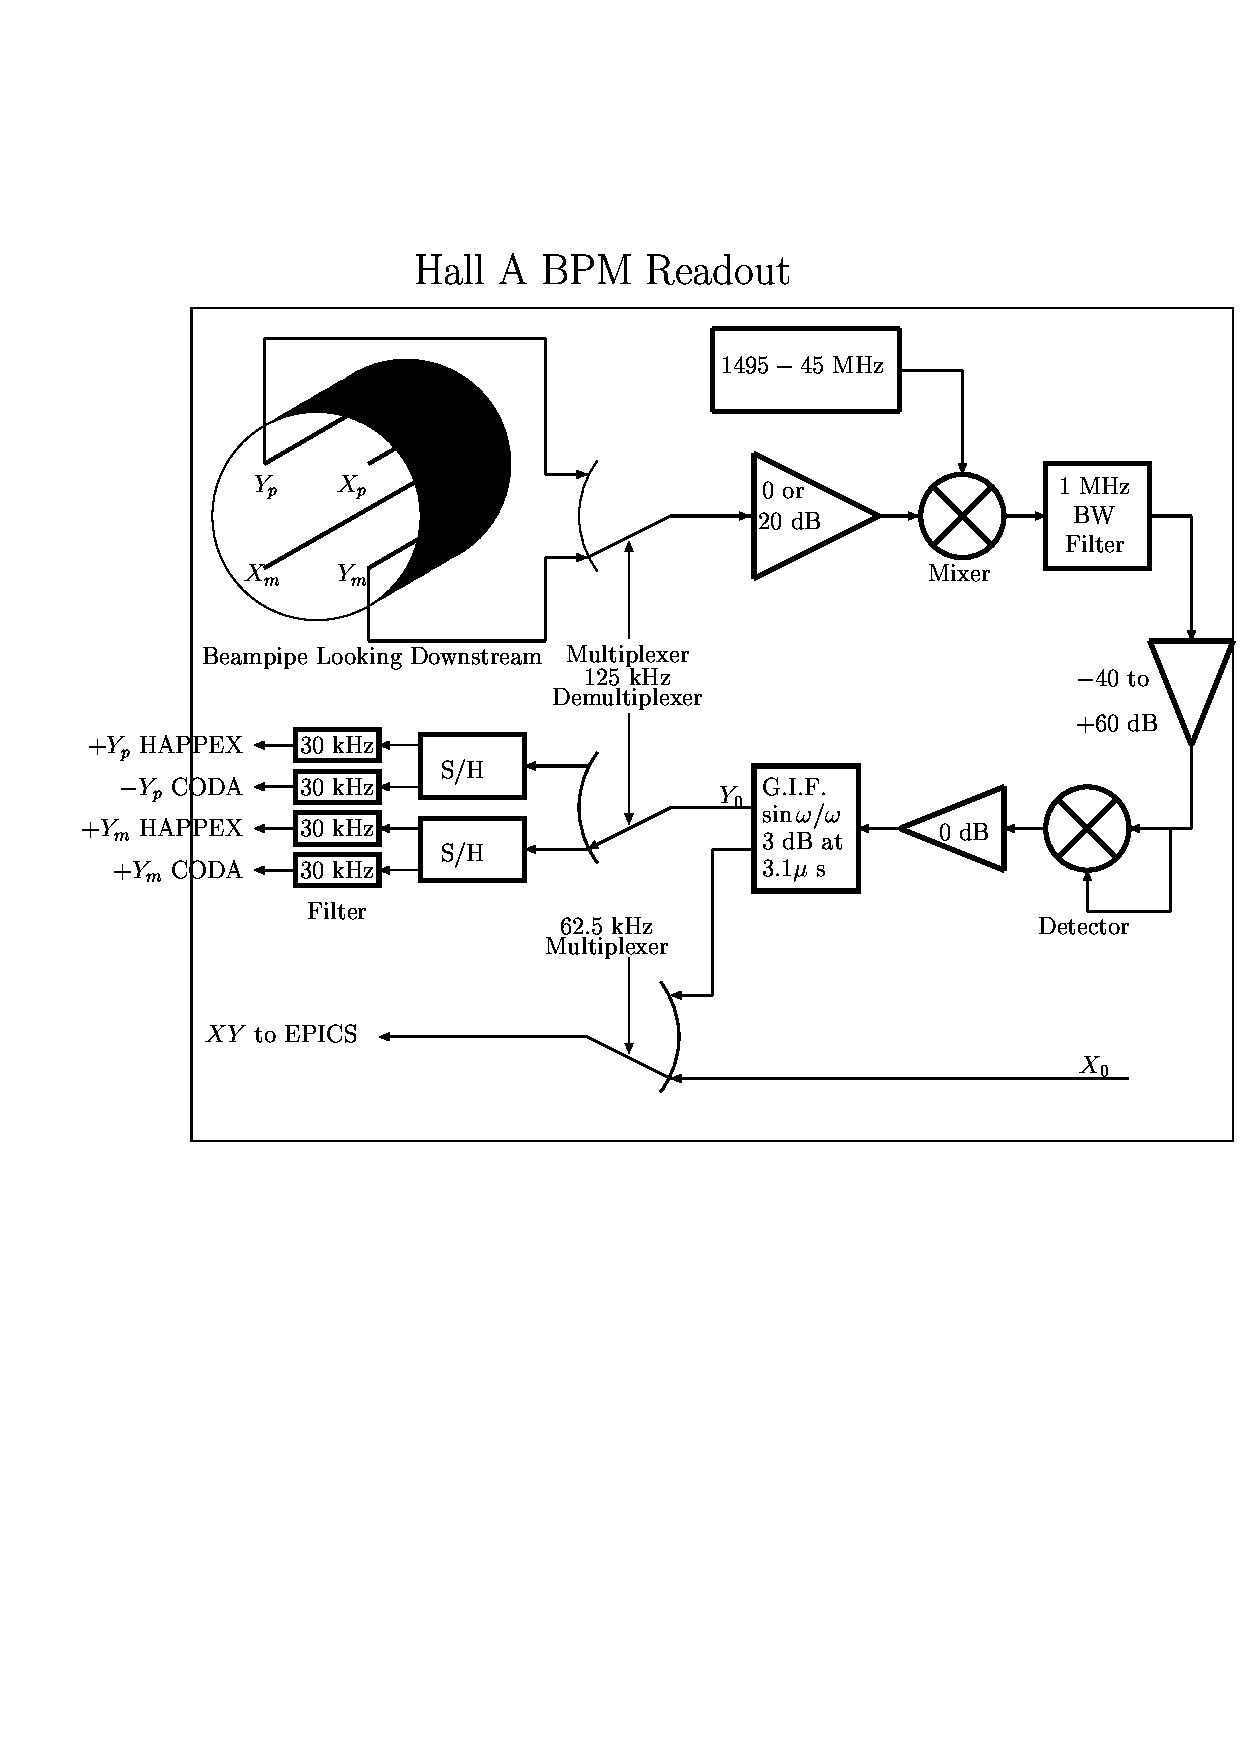
\includegraphics[angle=0,width=15cm]{BPM_fig}
{\linespread{1.}
\caption[Beamline: BPM Readout Electronics]{Schematic of the BPM readout
electronics}
\label{fig:bpmel}}
\end{center}
\end{figure}
}

1. The averaged position over 0.3 seconds is logged into the EPICS~\cite{EPICSwww} database (1 
Hz updating frequency) and injected into the datastream every 3-4 seconds, 
unsynchronized but with an orientative timestamp. From these values we can 
consider that we know the average position of the beam calculated in the EPICS 
coordinate system which is left handed.

2. Approximately once a shift (or more often if requested by the experimenters) 
a B-scope procedure ~\cite{bi:TP} can be performed using the same EPICS electronics 
which then gives the peak-to-peak variation of the beam.

3. Event-by-event information from the BPMs are recorded in the CODA datastream
from each of the 8 BPM antennas (2x4) from which the position of the beam can be 
reconstructed. However, these raw values belong to a parallel electronics chain 
whose constants have to be retrieved by calibrations to the EPICS or scanner 
data. 

\subsection{Beam Exit Channel}

After the target vacuum chamber, which was built by
the University of Virginia, there is an exit beam pipe which 
transfers the scattered beam onto the dump tunnel under vacuum. This exit beam 
pipe is made of a thin walled aluminum spiral corrugated pipe of welded 
construction. The largest diameter is 36 inches with a 0.164 inches wall 
thickness and the smallest diameter is 6 inches with a 0.042 inches wall 
thickness. The whole assembly is rather light (approximately 800 kg) and is 
supported by H shaped adjustable stands. To prevent possible linear collapse 
of the larger diameter sections under vacuum load, four aluminum channels of 
total cross-sectional area of 3'' are welded to its side. A vacuum of 
10$^{-5}$ Torr is maintained with a turbomolecular pump. The exit face of this 
pipe has a 12'' port and is connected to the diffuser with a Beryllium 
window.

}

\section{ Machine/Beamline protection system}
\label{sec:beam-fsd}

The MPS~\cite{MPScebaf} system is composed of the Fast Shutdown System (FSD), Beam Loss 
Monitor (BLM), and gun control system.

The FSD system is a network of permissive signals which terminate at the 
electron gun and chopper 1. The permissive to the gun and chopper
1 may be inhibited by any device connected to an FSD mode. Devices connected to the 
FSD system include vacuum valves, RF systems, Beam loss systems, beam current 
monitors, beam dumps, and particular to Hall A, the target motion mechanism 
and the raster (value and derivative).

The gun control system includes software program which monitors beam 
operating conditions and the state of the FSD and BLM systems. the program 
will warn the operators if a potential for beam damage exists. Potential for 
damage exists when running high average current beam, when FSD nodes are 
masked and when the beam power approaches the operating envelope limits for a 
specific beam dump.

\clearpage
\begin{safetyen}{10}{10}
\section{Safety Information}
\end{safetyen}
}
%
% Information for the ESAD
%

\begin{safetyen}{0}{0}

The beamline in the Hall provide the interface between the CEBAF accelerator
and the experimental hall.   All work on the beamline must be coordinated 
with both physics division and accelerator division; in order to ensure
safe and reliable transport of the electron beam to the dump.

\subsection{Hazards and Mitigations}

All magnets (dipoles, quadrupoles, sextupoles, beam correctors) and beam 
diagnostic devices (BPMs, scanners, Beam Loss Monitor, viewers) necessary for 
the transport of the beam are controlled by Machine Control Center (MCC) 
through EPICS~\cite{EPICSwww}, except for special elements which are addressed in the 
subsequent sections. The detailed safety operational procedures for the Hall 
A beamline should be essentially the same as the one for the CEBAF machine 
and beamline.\\ 

  
\noindent{}Personnel who need to work near or around the beamline should keep in mind the potential hazards:
\begin{itemize}
  \item Radiation ``Hot Spots'' - marked by ARM or RadCon personnel,
  \item Vacuum in the beam line tubes and other vessels,
  \item Thin windowed vacuum enclosers (e.g. the scattering chamber),
  \item Electric power hazards in vicinity of the magnets,
  \item Magnetic field hazards in vicinity of the magnets, and
  \item Conventional hazards (fall hazard, crane hazard etc.).
\end{itemize}

The most hazardous areas along the beamline are roped off it restrict access.   
In particule the scattering chamber, with it's large
volume and thin windows requires hearing protection once it has been evacuated.   
Signs are posted by radcon for any hot spots along the beamline and
radcon must be notified before work is done in a posted area.

Some magnets, as the M{\o}ller spectrometer elements, are covered with plastic
sheets for electric safety. Any access to these magnets requires
the ``Lock and Tag'' procedure~\cite{EHScebaf} and the appropriate training,
including the equipment-specific one. \\

\noindent{}Additional safety information is available in the following documents:
\begin{list}{--}{\setlength{\itemsep}{-0.15cm}}
  \item EH\&S Manual~\cite{EHScebaf};
  \item PSS Description Document~\cite{PSScebaf}
  \item Accelerator Operations Directive~\cite{AODcebaf};
\end{list}

\subsection{Responsible Personnel}

Since the beamline requires both accelerator and physics personnal to maintain
and operate and it is very important that both groups stay in contact that any 
work on the Hall A beamline is coordinated.

\begin{namestab}{tab:beam:personnel}{Beam line: authorized personnel}{%
   Beamline physics division and accelerator divison points-of-contact.}
  \namestabheader{Hall A Physicists}
  \DouglasHiginbotham{\em 1st Contact}
  \RobertMichaels{\em 2nd Contact}
  \namestabheader{Liaisons from Accelerator Division}
  \HariAreti{..to Physics}
  \YvesRoblin{..to Hall-A}
\end{namestab}
\end{safetyen}


\newpage
\section{ Beam Position Monitors}

To determine the position and the direction of the beam on the experimental 
target point, two Beam Position Monitors (BPMs) are located at distances 7.524 m 
(IPM1H03A) and 1.286 m (IPM1H03B) upstream of the target position. 
The BPMs consist of a 4-wire antenna array of open ended thin wire striplines 
tuned to the fundamental RF frequency of 1.497 GHz of the beam ~\cite{bi:bar90}. The 
standard difference-over-sum technique is then used ~\cite{bi:HW} to determine the 
relative position of the beam to within 100 microns for currents
above 1 $\mu $A. The absolute  position of the BPMs can be calibrated with respect to the 
scanners (superharps) which are located adjacent to each of the BPMs (IHA1H03A 
at 7.353 m and IHA1H03B at 1.122 m upstream of the target). The schematic of the 
readout electronics is shown in Figure ~\ref{fig:bpmel}. The
position information from the 
BPMs can be recorded in three different ways:

\begin{figure}
\begin{center}
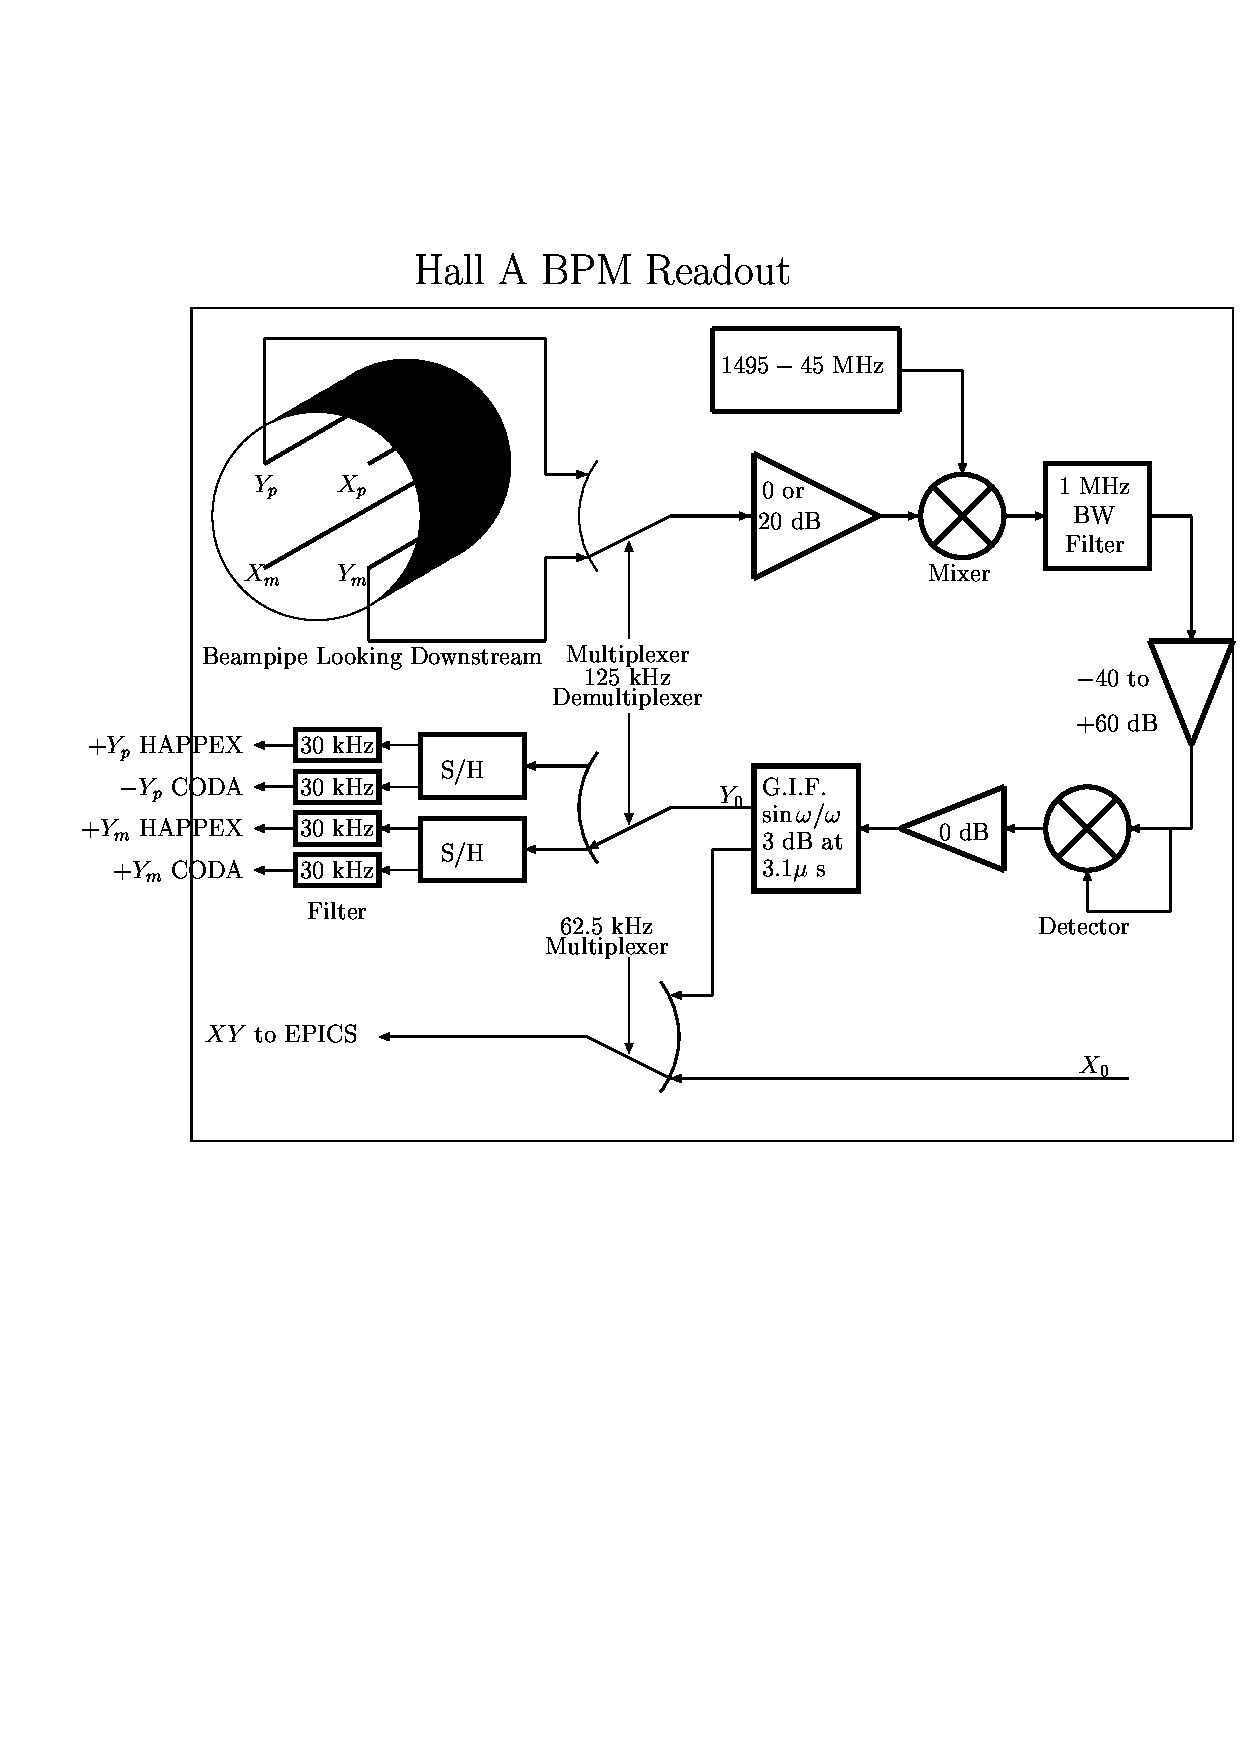
\includegraphics[angle=0,width=15cm]{BPM_fig}
{\linespread{1.}
\caption[Beamline: BPM Readout Electronics]{Schematic of the BPM readout
electronics}
\label{fig:bpmel}}
\end{center}
\end{figure}

\vskip 0.5cm

1. The averaged position over 0.3 seconds is logged into the EPICS database (1 
Hz updating frequency) and injected into the datastream every 3-4 seconds, 
unsynchronized but with an orientative timestamp. From these values we can 
consider that we know the average position of the beam calculated in the EPICS 
coordinate system which is left handed.

\vskip 0.5cm

2. Approximately once a shift (or more often if requested by the experimenters) 
a B-scope procedure ~\cite{bi:TP} can be performed using the same EPICS electronics 
which then gives the peak-to-peak variation of the beam.

\vskip 0.5cm

3. Event-by-event information from the BPMs are recorded in the CODA datastream
from each of the 8 BPM antennas (2x4) from which the position of the beam can be 
reconstructed. However, these raw values belong to a parallel electronics chain 
whose constants have to be retrieved by calibrations to the EPICS or scanner 
data. 


%\begin{thebibliography}{99}
%\bibitem{bi:bar90} W. Barry et al., CEBAF-PR-90-009 (1990).
%\bibitem{bi:HW} C. Hyde-Wright et al., Beam Position Studies for E93050 and priv. comm..
%\bibitem{bi:TP} T. Powers, priv.  comm.. 
%\end{thebibliography}
% ===========  CVS info
% $Header: /group/halla/analysis/cvs/tex/osp/src/beamline/bpms.tex,v 1.1 2003/06/05 17:28:32 gen Exp $
% $Id: bpms.tex,v 1.1 2003/06/05 17:28:32 gen Exp $
% $Author: gen $
% $Date: 2003/06/05 17:28:32 $
% $Name:  $
% $Locker:  $
% $Log: bpms.tex,v $
% Revision 1.1  2003/06/05 17:28:32  gen
% Initial revision
%

\newpage
\section[Beam Current Measurement]{Beam Current Measurement
\footnote{
  $CVS~revision~ $Id: bcm.tex,v 1.5 2003/12/13 06:23:37 gen Exp $ $
}
\footnote{Authors: A.Saha \email{saha@jlab.org}}
}

The Beam Current Monitor (BCM) is designed for stable, low noise, non-intercepting 
beam current measurements. It consists of an Unser monitor, two rf cavities, 
the electronics and a data acquisition system. The cavities and the Unser monitor 
are enclosed in a box to improve magnetic shielding and temperature stabilization.
The box is located 25 m upstream of the target. You can recognize it as a grey 
object on the stands, about 2 m downstream from where the beam enters the 
hall. 

The DC 200 down-converters and the Unser front end electronics are located in Hall 
A. The temperature controller, the Unser back end electronics and its calibration 
current source, cavity's RF unit (housing the RMS-to-DC converter board) and all 
multi-meters, VME crate and computers are located in Hall A control room.

\infolevone{
\subsection{ System Layout}

The schematic diagram of the BCM system is presented in
Fig.~\ref{fig:halla_bcm}.
\begin{figure}[htp]
\begin{center}
\includegraphics[angle=0,width=0.9\textwidth,clip]{habcm_r}
{\linespread{1.}
\caption[Beam Current Measurement: Schematic]{Schematic of the Hall A beam
current measurement system.}
\label{fig:halla_bcm}}
\end{center}
\end{figure}

The Unser monitor is a Parametric Current Transformer designed for non-destructive 
beam current measurement and providing an absolute reference. The monitor is 
calibrated by passing a known current through a wire inside the beam pipe and has a 
nominal output of 4 mV/$\mu $A. It requires extensive magnetic shielding and 
temperature stabilization to reduce noise and zero drift. As the Unser monitor's 
output signal drifts significantly on a time scale of several minutes, it cannot be 
used to continuously monitor the beam current. However, this drift is measured 
during the calibration runs (by taking a zero current reading) and removed in 
calibrating the cavities.  The more stable cavities are then used to determine the 
beam current and charge for each run. We also use the OLO2 Cavity Monitor and the 
Faraday Cup 2 at the Injector section to provide an absolute reference during 
calibration runs.

The two resonant rf cavity monitors on either side of the Unser Monitor are 
stainless steel cylindrical high Q ($\sim 3000$) waveguides which are tuned to the 
frequency of the beam (1.497 GHz) resulting in voltage levels at their   outputs 
which are proportional to the beam current. Each of the rf output signals from the 
two cavities are split into two parts. One part of the signal is  converted to 10 
kHz signals (by the ``downconverters'') and fed into an RMS-to-DC converter board 
consisting of a 50 kHz bandpass filter to  eliminate noise, amplified and split to 
two sets of outputs, which after further processing are recorded in the data 
stream. These two paths to the data stream (leading to the sampled and integrated
data ) will now be described. (The other part of the split signal is downconverted 
to 1 MHz signals and represents the old system (pre Jan 99). Only the HAPPEX 
collaboration presently uses these signals.)

For the sampled (or EPICS~\cite{EPICSwww} or Slow) data, one of the amplifier outputs is sent to a 
high precision digital AC voltmeter (HP 3458A). Each second this device provides 
a digital output which represents the  RMS average of the input signal during that 
second.  The resulting number is  proportional to the beam charge accumulated 
during the corresponding second (or, equivalently, the average  beam current  for 
that second). Signals from both cavity's multi-meters, as well as from the 
multi-meter connected to the Unser, are transported through GPIB ports to the HAC 
computer where they are recorded every 1 to 2 seconds via the data-logging process 
which is described in the calibration procedure. They are also sent through EPICS 
to CODA and the data stream where they are recorded at  quasi-regular intervals, 
typically every two to five  seconds.

For the integrated (or VTOF or Fast) data, the other amplifier output is sent to an 
RMS-to-DC converter which   produces  an analog DC  voltage  level. This level 
drives a Voltage-To-Frequency (VTOF) converter whose output frequency is  
proportional to the  input DC voltage level. These signals are then fed to Fastbus  
scalers and are finally injected into the data stream along  with the other scaler 
information.  These scalers simply accumulate during  the run, resulting  in a 
number which is proportional to the time integrated voltage level and therefore 
more accurately represents the true integral of the current and hence the total 
beam charge. The regular RMS to DC output is linear for currents
from about 5 $\mu$A to somewhere well above 200 $\mu$A.
 Since it is non-linear at the lower 
currents, we have introduced a set of amplifiers with differing gains (x3 and x10) 
allowing the non-linear region to be extended to lower currents at the expense of 
saturation at the very high currents. Hence there are 3 signals coming 
from each BCM (Upx1, Upx3, Upx10, Dnx1, Dnx3, Dnx10). All 6 signals are fed 
to scaler inputs of each spectrometer (E-arm and H-arm) . Hence we have a 
redundancy of 12 scaler outputs for determining the charge during a run. During 
calibration runs we calibrate each of these scaler outputs.   
}

\begin{safetyen}{10}{10}
\subsection{ Authorized Personnel}
\end{safetyen}

All Hall A members are authorized to take BCM calibration data using the Standard 
Non-Invasive Hall A BCM Calibration Procedure. The extended calibration procedures 
involving the Faraday Cup 2 and the OLO2 monitor at the Injector are presently 
performed by A. Saha. 

\vskip 0.2cm

The Accelerator AES group performs the maintenance of the BCM monitors. These 
include:

\begin{tabular}{l l}
1. The Unser calibration. & Every 3 months \\
2. Resonant Cavities Tuning. & Every Downtime \\
3. Multi-meters Autocalibration. & Every Downtime \\
4. Connectors Cleaning. &  Every year \\
5. Unser Keithley Current Source. & Calibration Yearly \\
6. Digital Multi-meters HP3458A and HP 34401A. & Calibration Yearly\\   
\end{tabular}

System Contacts are shown in Table~\ref{tab:BCM:personnel}.
\begin{namestab}{tab:BCM:personnel}{BCM: authorized personnel}{%
   Beam Current Monitor: authorized personnel}
  \ArunSaha{\em Contact}
  \JohnMusson{Accel. expert}
\end{namestab}
%Jean-Claude Denard -x 7555




% ===========  CVS info
% $Header: /group/halla/analysis/cvs/tex/osp/src/beamline/bcm.tex,v 1.5 2003/12/13 06:23:37 gen Exp $
% $Id: bcm.tex,v 1.5 2003/12/13 06:23:37 gen Exp $
% $Author: gen $
% $Date: 2003/12/13 06:23:37 $
% $Name:  $
% $Locker:  $
% $Log: bcm.tex,v $
% Revision 1.5  2003/12/13 06:23:37  gen
% Septum added. Name tables. Polishing
%
% Revision 1.4  2003/12/05 05:48:30  gen
% Polishing
%
% Revision 1.3  2003/06/06 15:19:02  gen
% Revision printout changed
%
% Revision 1.2  2003/06/05 23:29:59  gen
% Revision ID is printed in TeX
%
% Revision 1.1.1.1  2003/06/05 17:28:32  gen
% Imported from /home/gen/tex/OSP
%
%  Revision parameters to appear on the output

\newpage
\section[Fast Raster]{Fast Raster
\footnote{Authors: R.~Michaels \email{rom@jlab.org}}
}


The beam is rastered on target with an amplitude of
several millimeters at 25 kHz to prevent overheating.  
The raster is a set of four of air-core dipoles located
approximately 23 m upstream of the target. 
Two dipoles are for horizontal (X) motion and
another two for vertical (Y).  During the 6 GeV era
there was only one pair of X and Y, but we have doubled
the raster to account for the energy increase to 11 GeV.
The arrangement along the beamline along the 
direction of the beam will be XXYY.

For a typical 40A current in the raster coils, the
deflection by one pair (e.g. the X direction) of coils, 
in radians, is $\theta = 1.94 \times 10^{-3}/ E$
where $E$ is the electron's energy in GeV.
For example, at $E = 6$ GeV, a 0.32 mrad deflection is achieved.
Projected onto the target (about 21 m away) this is a $\pm$ 6.8 mm
excursion {\it if} there were no other magnetic fields 
between the raster and the target; however, there are quadrupoles
which change this depending on the beam tune.

Since 2003 we've used the triangle-wave 
raster pattern designed by Chen Yan.  
This achieves a very uniform rectangular
density distribution of beam on the target 
by moving the beam with a time-varying dipole
magnetic field whose waveform is triangular
with very little dwell time at the peaks.  
The electronics design is an ``H-bridge''
in which switches are opened and closed 
at 25 kHz, to switch between two directions 
of current (100 A peak-to-peak) 
through the raster coils.

Three new features during the 12-GeV era are 
1) the driver of the H-bridge electronics is now
an Agilent model 33522A waveform generator; and
2) The two X are synchronized with each other, and
the two Y are synchronized.  This makes the kicks
add and allows us to accomodate the higher energy
of the beam; and 3) The entire raster can
be synchronized to an external 10 MHz wavetrain
supplied by the polarized injector electronics.
This makes the nominal 25 kHz an exact multiple of
the helicity-flip rate, which achieves a cancellation
of raster noise, important for parity-violation 
experiments only.
The syncrhronization of the pairs of X and Y are
accurate to within a few nsec.

For most users, these three new features will not be
noticeable and the raster will appear to function
the same as during the 6 GeV running.
A user can view the 
status of the raster in the
EPICS overview screen called ``General Accelerator
Parameters'' where the set-point for the radius amplitude
and the readback of the peak-current in the raster are displayed.

Control of the raster is done by first asking the MCC
operators to set up the raster for a particular size
typically 2 mm square.
The control software assumes a field-free region between
the raster and the target, so it is only approximately
correct because there are several quadrupoles in this region.
It is important to check the raster spot size and
make adjustments if necessary.  The adjustment is made
by asking MCC to change the size and noting the 
linear relationship between what their software says
the size is and the actual size.
Relatively small independent adjustments to the 
gains on the X and the Y raster
coils are available in the middle room of the hall A
counting room using the ``PGA Controller'' knobs;
however, it is not recommended to touch these.
Near these knobs is also located an oscilloscope X-Y trace
of the current in the raster.  A fast shutdown (FSD) shuts
the beam down within 0.1 msec if the raster fails, thus
affording some protection of the target.

{\it NOTE:  If you are unsure of the status of the raster,
measure the spot size with very low current ($\le 2 \mu$A) or with
the target out of the beam.}  It would be a mistake
to check the beam spot size with high current on target; by
the time you check it, the target may already be destroyed.
The rastered beam spot on target can be checked with
plots in the ROOT analyzer or by 
using the stand alone code called \mycomp{spot},
also called \mycomp{raster}.
For more details on usage, type \mycomp{spot -h} (help)
on the ADAQ computers.

Regarding the BPM measurements, it should be noted that 
the stripline BPMs displayed by \mycomp{spot} have a high-frequency 
cutoff of approximately 30 kHz.  Since the raster frequency is 25 kHz
the plot of the amplitude distribution shows spikes at the 
limits of the orbit, instead of a flat distribution.  The scale
factor between what is seen in \mycomp{spot} and the real width of the beam
is $\sim 1.5$, i.e. the beam is 1.5 times bigger than the naive
reading of the \mycomp{spot} distribution.



\newpage
% Updated Comments Dec. 2
\infolevone{
\chapter[Arc Energy Measurement]{Arc Energy Measurement
\footnote{Authors: D. Higinbotham \email{doug@jlab.org}}
}
}

\infoleveqnull{
\section{Arc Energy Measurement}
\subsection{Overview}
In order to determine the integral field of the eight dipoles that lead to Hall A, and 
in turn determine the beam energy, a nineth dipole wired in series with the rest is 
located in a special shed near the hall A counting house.
}

\infolevone{
The ARC energy measurement is under EPICS~\cite{EPICSwww} control through 
a MEDM~\cite{MEDMwww} display. Two
independent control systems are used: the beam bend angle measurement through
the arc ("scanners") and the field integral of
the arc ("integral"). To measure the energy: 

\begin{itemize}
\item perform several angle measurements 
\item perform an integral measurement 
\item analyze the integral measurement and note the value of the arc field 
integral 
\item analyze the angle measurements, average the results (proposed by the 
software),
then ask for the energy calculation, enter the above arc field integral and
you will get the beam energy computed from the average angle. 
\end{itemize}

\section{Summary of ARC operations }

Six scanners of the same type, called ``ARC scanner'' and labelled
from scanner \#1 to \#6, are installed on the Hall-A beamline. Scanners \#1
to \#4 are used for the ARC energy measurement and they are located on the Hall-A
arc: \#1 [1HA1C07A] and \#2 [1HA1C07B] just upstream of the arc, in the BSY, and 
\#3 
[1HA1C18A] and \#4 [1HA1C18B] in the Hall-A
tunnel, just upstream the Compton polarimeter. Scanners \#5 [1HA1H03A] and \#6 
[1HA1H03B] 
are located
between the Moller and the target to control the beam geometry on the target
and their use will not be discussed here. 

Procedure for running a harp scan is described elsewhere\footnote{
Harp scan procedure \url{http://hallaweb.jlab.org/equipment/beam/harp_halla/harp.html}.}

Each scanner has a motor/ball-screw/shaft-encoder/vacuum-penetrator system moving
accurately a set of 3 tungsten wires through the beam. Each time a wire crosses
the beam a PMT located a few meters downstream records a signal due to the 
electromagnetic
shower induced by the beam in the wire. Both forward and backward passes are
recorded. The motion is a horizontal translation and, for a forward pass: 

-the translation is from beam left to beam right, 

-the two first wire crossing the beam are at 45deg from the vertical, 

-the third wire, which is the only important for the ARC energy measurement,
is vertical. 

Recording, during the scan, the scanner position and the PMT output voltage
allows us to determine the beam position at each scanner location. Then, using
calibration data not detailed here, we deduce the net beam bend angle through
the arc. This result measured in dispersive arc tuning, along with the field
integral of the arc dipoles, provides an accurate determination of the beam
energy. 

\vspace{0.3cm}

\section{Summary of field integral }

The purpose is to measure absolutely the straight field integral of a 
"BA"
3m long dipole, called the "9th dipole" and located in the
"Dipole Shed". It is of the same type as the 8 arc dipoles
and is powered in series with them. 

The ARC integral setup is basically made of a 3m long plate (the 
"probe")
which is able to move inside the 9th dipole gap along the beam axis and carrying 
two
field measurement devices: a pair of pick-up coils connected in series and a
set of NMR probes. The coils are on both ends of the probe and the NMRs close
to the center. 

-at the "upstream" probe position, the 
"downstream"
coil is close to the dipole center, the "upstream" is outside
the dipole and the NMRs at one end of the dipole: 

Door$<-$-- ....................$<-$-------DIPOLE-----$--->$ 

.............$<-$-------PROBE------$--->$ 

-at the "central" probe position, each coil is at one end
of the 3m long dipole and the NMRs close to the dipole center: 

Door$<-$-- ...................$<-$-------DIPOLE-----$--->$ 

..................................$<-$-------PROBE------$--->$ 

-at the "downstream" probe position, the 
"upstream"
coil is close to the dipole center, the "downstream" is outside
the dipole and the NMRs at one end of the dipole: 

Door$<-$-- ...................$<-$-------DIPOLE-----$--->$ 

....................................................$<-$-------PROBE------$--->$ 

We call upstream the position where the probe is the closest to the shed access
door. Among the 3 above positions, the only one where the NMR can lock on the 
dipole
field is the central one as in the extreme position of the probe, the field 
homogeneity
is not sufficient. The probe position is controlled by a linear encoder. The
Z axis refers to the "beam" direction, increasing from upstream
to downstream. We use three kinds of "Z": 

-Zm to locate a point inside the magnet. The dipole center is at Zm=0 and the
yoke ends at +-1500.mm 

-Zp to locate a point inside the probe. The probe center is at Zp=0. Each of
the 4 NMR probes has a Zp given in the file "magnet.dir".
At a temperature of 21C, the coils are at Zp=+-1519.815mm (from magnet.dir) 

-Zd to refer to a displacement of the probe w.r.t. the dipole. Zd=0 refers to
the upstream (home) position of the probe. The integral measurement is performed
from Zd=0.000mm (1st PDI trigger) to Zd=3199.000mm (last PDI trigger), for forward
pass. Zd is given by the display (at the top of the rack) or by the master screen
("OUT"). 

The relationship between Zm, Zp and Zd is: 

Zd-Zm+Zp=C 

where C is a constant given in magnet.dir (C=1604.000 nomin.). Example of use:
to have the probe center at the dipole center, one must set Zd=1604.000mm (set
Zm=0 and Zp=0 in the above formula, and solve for Zd) 

The integral measurement sequence is the following: 

-from the current position (a priori arbitrary) move the probe upstream, up
to a limit (optic) switch. 

-move downstream by a few mm to cross the encoder index (encoder initialization) 

-move to the central position to measure the central field by NMR, the system
checks if the NMR locks and if the reading is stable, it will be the 
"before"
field 

-move back to upstream position 

-move to downstream position while integrating the flux through the coil system,
this measurement will be called the "forward" integral (duration
\( \sim  \) 7s) 

-move back to upstream position while integrating the flux through the coil
system, this measurement will be called the "backward" integral
(duration \( \sim  \)7s) 

-move to the central position to measure the central field by NMR, the system
checks if the NMR locks and if the reading is stable, it will be the 
"after"
field. 

In addition to the central field, 4 probe temperatures, a local excitation current
measurement, the setting of the dipoles P.S, the readback of the dipoles P.S
and the probe position at NMR measurement time are recorded 
"before"
and "after". 

To perform an integral field measurement: 

1-check if the system works (see "details on integral system 
check"
below) 

2-run the above integral sequence (see "details on integral run"
below) 

3-fix the error(s) if any (see "details on integral errors"
below) 

4-save the data in a file (see "details on integral data save"
below) 

5-analyze the data  


\section{Details on integral run }

To run the integral measurement sequence, call the 
\mycomp{arc\_integral.adl}
medm screen, then: 

-push "start" to start the full sequence 

-look at the results displayed: 

-after the "before" NMR measurement: the 
"before"
data set 

-after the "forward" integral pass: the forward velocity profile
and the forward voltage-after-gain profile 

-after the "backward" integral pass: the backward velocity
profile and the backward voltage-after-gain profile 

-after the "after" NMR measurement: the 
"after"
data set 

-if "BAD NMR" or "PDI saturation" flags
are set, or if something is obviously wrong in the data or plots, call expert. 

-data are ready to be saved (see "Details on integral data save"
below) 


\section{Details on temperatures }

The AC system of the shed is made of two cooling units, a heating unit and a
controller connected to two temperature sensors : one located in the shed and
one located in the BSY. This system is programmed in such a way that the 
temperature
of the shed follows the BSY temperature within +-2C. The BSY temperature can
be anywhere in the 18C to 35C range, regardless of the season. The BSY 
temperature
and the shed temperature are given (in F) by a display panel located close to
the workstation, on the wall. The AC system can be set in manual control by
turning from "auto" to "manual" a set of
switches controlling the cooling units and the heater unit. These switch boxes
are located on the shed wall. If the shed temperature is above 34.4C (94F),
call the crew chief (the electronics can be damaged) and cool down the shed in manual
AC mode. The 4 temperature sensors of the probe are labelled Tx+z+, Tx+z-, Tx-z+,
Tx-z- depending on their position w.r.t. the frame. 

Both "x+" sensors are on the probe edge which is inside the
dipole gap and both "x-" sensors on the opposite edge which
is outside the dipole gap. Both "z-" sensors are at 1/4 of
the long dimension of the probe and both z+ at 3/4 of this length. The average
of the 4 temperatures is used by the analysis program to correct the coil distance
from the thermal expansion of the probe, so it is important to make sure that
the 4 sensors are working well. The user can just make sure that the temperatures
displayed in \mycomp{arc-master.adl} or recorded in 
\mycomp{arc-integral.adl}
are realistic. In \mycomp{arc-integral.adl} they are given in the
order: Tx+z-, Tx+z+, Tx-z-, Tx-z+ Tx-z- and Tx-z+ should be close to the shed
temperature. Tx+z- and Tx+z+ depend on the probe position, as the gap (iron
yoke) is warmer than the shed and the dipole coil (at both ends of the dipole)
is warmer than the iron yoke. For a probe in a central position for more than
about one hour, the Tx+z- and Tx+z+ sensors should give the yoke temperature,
i.e the shed temperature plus 0. to 5.C, depending on the current, LCW temperature
and the magnet/shed temperature history. The 4 temperatures are also displayed
inside the shed, on the electronics rack. These values are digitized by separate
ADCs, so they may differ from the remote values by \( \sim  \)0.1C. 
}

\begin{safetyen}{10}{10}
\infolevone{\section{Shed access and safety }}

Due to the the dipole magnet and motion system, the access to the shed is limited to authorized
persons which are listed in the ESAD and listed below. To be added to the list, 
contact Douglas Higinbotham.
The standard
operation mode of the integral measurement setup is the remote mode, through
the network, from the counting house.
\end{safetyen}

\begin{safetyen}{10}{10}
\infolevone{\section{List of Authorized Personnel for Shed Access}}
\infoleveqnull{\subsection{List of Authorized Personnel for Shed Access}}
\end{safetyen}
\begin{namestab}{tab:arc:personnel}{Arc Energy Measurement: authorized personnel}{%
                 Arc Energy Measurement: authorized personnel}
  \namestabheader{Hall A Personnel}
  \DouglasHiginbotham{\em Contact}
  \namestabheader{Accelerator Personnel}
  \MichaelTiefenback{}
  \YvesRoblin{}
  \RickGonzales{}
  \BillMerz{}
  \MarkAugustine{}
  \HariAreti{}
  \PeteFrancis{}
  \ScottHiggins{}
  \DavidSeidman{}
  \RonLauze{}
  \TonyDay{}
  \ChristopherCurtis{Alignment group}
  \namestabheader{CEA - Saclay experts}
  \PascalVernin{}
  \ChristianVeyssiere{}
  \FrancoisGougnaud{}
  \JacquesMarroncle{}
\end{namestab}



\newpage
\infolevone{
\chapter[Target Chamber]{Target Chamber
\label{sec:target_chamb}
\footnote{
  $CVS~revision~ $Id: tgtcham.tex,v 1.11 2005/04/04 22:27:25 gen Exp $ $
}
\footnote{Authors: ?? \email{??@jlab.org}}
}

The cryo-targets and the waterfall targets 
(see Sec.~\ref{sec:targets-overv}) 
are contained in a special target chamber which is a large 
evacuated  multistaged can. So far, three chambers have been designed:
\begin{list}{\arabic{enumi}.~}{\usecounter{enumi}\setlength{\itemsep}{-0.15cm}}
  \item a chamber used up to 2003;
  \item a chamber designed for use with septum magnets, starting in 2003;
  \item a chamber designed for use with the BigBite spectrometer.
%\footnote{
%        No yet manufactured by Dec,2003.}.
\end{list}

Here, chamber 1 is described. Chambers 2 and 3 are only different in 
size and slightly in shape. The safety considerations fully apply to chambers 2 and 3.
The chamber was designed to isolate the beam line vacuum from  each
HRS so that each HRS could rotate
around the target without vacuum coupling and without jeopardizing
certain desired kinematic and acceptance  specifications of 
both high resolution spectrometers
needed for approved experiments.  It  was also designed to simultaneously
 contain a liquid or gas target and an array of water cooled thin
 metallic foils, both remotely controlled and also be adaptable for
the waterfall target. The desired kinematic specifications that were
 considered included momentum and energy resolution in both arms,
 angular range of spectrometers, angular acceptance, and luminosity.
The chamber vacuum is isolated from the  HRS by using thin aluminum foils. 

The target chamber is designed so that
each spectrometer will have continuous coverage in the standard tune from
$\theta_{min}=$12.54$^\circ$ to $\theta_{max}=$165$^\circ$.
The aluminum window is 6~$in$ high and 0.016~$in$ thick made of 5052 H34 aluminum foil.
The foil forms regularly spaced vertical ridges when
placed under load. The window had an inter-ridge
spacing of 3 inches.
If the window is treated as a collection
of smaller rectangular windows which have the full vertical height
of 6 inches and the inter-ridge spacing as a width,
then stress formulas predict that the 0.016 $in$
material would reach ultimate stress at a pressure higher than 35 PSID
(for both over-pressure and under-pressure). 
There is a gate valve between the 
scattering chamber and the beam entrance (exit) 
pipe. Both 
valves will be closed automatically in the
event that the chamber vacuum begins to rise and an FSD will be caused
( this is done via a relay output of the scattering
chamber vacuum gauge). If either valve is closed an FSD will result.

The target chamber is supported by a 24 $in$ diameter pivot post
secured in concrete, rising about 93.6 $in$ above the Hall A cement floor.
The Hall A target chamber
consists of an aluminum middle ring, a stainless steel base ring,
each with a 41.0 $in$ inner diameter,
and a stainless steel cylindrical top hat with 40 $in$ inner diameter
to enclose the cryotarget and secure the cryogenic connections.

When the scattering chamber is under vacuum, there is a potential
danger of window rupture.
The loud noise from the rupture could hurt
one's ears if not protected. Therefore when the chamber is under vacuum,
protective covers are put on if possible. These must be taken off
for data taking. For restricted access, the protective cover is required
to be on when the chamber is under vacuum. Before switching from controlled
access to restricted access, the protective cover is required to be installed.
Anytime that the scattering chamber
is under vacuum, the pivot area is enclosed in a rope or tape barrier
and a warning sign is posted.
Hearing protection is required in the enclosed area.

\infolevone{
	The aluminum ring with an outer diameter of 45.0 $in$ and
wall thickness 2.0 $in$  is necessary for a sturdy support structure and
to permit machining of the outside surface to accommodate
the flanges for fixed and sliding seals mounted on
opposite sides of the ring that vacuum connect the chamber to each HRS.
The height of the aluminum ring shown is 36.0 $in$, which is
designed to accommodate the mounting flanges.
The stainless steel base ring 
is 11.50 $in$ in height with
one pump-out 6 $in$ diameter port  and with
seven 4 $in$ viewing and electrical feed-through ports.
The base ring will also contain support mechanisms for the solid
target ladder assembly, a rotisserie for collimating slits, radiators, and
magnetic
fingers for
removing the solid target vacuum-lock can. The total height of the top
ring, middle ring, and
base ring is 93.81 $in$. This length is partly determined by our desire to
include with the cryogenic extended target a solid target vertical ladder
secured in an inverted hat through a hole in the base of the chamber.

	The base ring includes an end plate through which the
inverted hat will be adapted to fit into the large vertical pipe serving
as the pivot post for the Hall A spectrometers.

	The stainless steel cylindrical top hat  has
40.0 $in$ inner diameter, and is 0.375 $in$ thick and
46.31 $in$ high , which is necessary to permit the
cryotarget to be withdrawn and to make space available to expose the solid
targets to the electron beam.

   The 200 $\mu$A electron beam, focused to a $\sim$\(0.1\, mm\times
0.1\) mm spot and rastered $\pm$5 mm horizontally or vertically on the
target, enters through a oval hole in the middle ring which
is 2.06 $in$ wide and exits through a 1.81 $in$ hole connected to the
exit pipe.
}

\infolevone{
\section{Target Chamber - Spectrometer Coupling}

   The aluminum middle ring will support a flange on each side for each high
resolution spectrometer. Four flanges will be available: Two flanges will
contain a 6 $in$ window opening which will be covered with a thin foil
(e.g., 10 mil aluminum) .
These two flanges will be used for experiments utilizing
extended  targets that do not require optimum momentum resolution.
The other two flanges will have two fixed ports (with a 8 $in$ $\times$ 6 $in$
opening)
which will be mainly used for calibration of the spectrometers . Fixed ports are
centered at 16.11 $^\circ$ and
45 $^\circ$ for one flange and at 16.11 $^\circ$ and 90 $^\circ$ for the second
flange.

   For a point beam on target a vertical opening in the walls of the chamber
of height 57.15 cm x 0.065 x 2 = 7.43 cm is required so that the scattered
beam is within the full acceptance of the spectrometer.
If the beam is rastered on target $\pm$0.5 cm in the vertical direction,
then the opening in the outer side of the chamber must be at least 8.5 cm for
full acceptance.

From consideration of the angular range of the spectrometers in the standard
tune, the scattered beam acceptance envelope, the effects of an
extended gas target on acceptance,
and the effects of a rastered beam $\pm$ 5 mm on acceptance,
the target chamber requires a window of at least 8.5 cm
high in the aluminum ring extending from 6.33 $^\circ$ (2.48 in) from the
beam exit point to 8.83 $^\circ$ (3.47 in) from the beam entrance point on one
side and a similar window on the other side of the beam.
For future considerations (e.g., using a third arm or sliding seal) the
width of the window on the middle ring was actually constructed
to be 17.78 cm (7 $in$).

\section{Stress Analysis of the Middle Ring}

Since the middle ring has an extensive cut across the midplane on both sides as
well as
entrance and exit holes and loaded with about 25,000 lbs, calculations of the
stresses
 and deformation of  the
midplane support area of the middle ring and deflection of the window opening
were made using the finite element analysis code ANSYS . The work was conducted
by a graduate student in the Department of Civil Engineering at the
University of
Virginia and a REU student.  A scaled down model of the middle ring was
constructed and then tested by applying forces to it using the Materials Testing
Service of the Department of Transportation at the University. ANSYS was first
checked by comparing calculations of the test model deflections to the actual
data. Agreement was  within $\pm$10\%. Results of ANSYS for the target
chamber showed that the maximum deflection of the opening of the window in the
middle ring varied from 0.007 $in$ to 0.015 $in$ depending on how the
middle ring
was loaded. This was decided to be a safe limit. In the final design, several
movable
7 $in$ long, 2 $in$ diameter aluminum support rods are placed in the
window for added support. In addition, flanges defining the ports and
coupling to
the spectrometers can be added, giving additional support to the middle ring.
Compressional stresses, calculated using ANSYS assuming the middle ring was
attached to the
top hat and loaded with 25,000 lbs, were less than 3000 psi 
almost everywhere.
However, stresses over small areas rose to levels 6000 psi near the entrance
and exit holes. These calculations indicated that we did not exceed the safety
limit of 15,000 psi for aluminum. A simple model calculation shown in Appendix
A  gives the result 1434 psi, which represents some average value over the
midplane
contact area.

\section{Vacuum Pumping System}

The vacuum in the target chamber is maintained by an Alcatel ( 880 l/s)
 turbomolecular vacuum pump. The pump is connected to a 6 $in$ port in the
stainless steel ring between 130
 $^\circ \le \theta_p \le 180 ^\circ$. The vacuum pump is
fastened to a horizontal pipe connected to the chamber. The vacuum pressure in
the chamber is about $10^{-5}$ mm. An additional Alcatel pump connected
to an 8 $in$ port should be added to obtain lower vacuum. Both
pumps may be isolated
from the target chamber using gate valves which are remotely operated
from the vacuum control rack and interlocked to the FSD system.


A 2 $in$ all metal gate valve is located between the entrance flange to the
chamber and the beam profile monitor.   
 An additional gate valve is located 2 m downstream of the
 target chamber to isolate the chamber from the exit beam pipe.
}
\begin{safetyen}{10}{15}
\section{Safety Assessment}
\end{safetyen}

The scattering chamber is typically a low maintenance item but it is a vacuum
system and hence problems may occur. The day to day operations of the cryogenic
targets are managed by the Hall A Staff while major maintenance operations are
handled by the Cryogenic Target Group (Physics Division). Occasionally the
cryogenic targets experience difficulties due to failures of the End Station
Refrigerator which supplies the coolant. In these cases the Cryogenics Group
of the Accelerator Division should be contacted.

\noindent{}The target chamber may pose several hazards:

\begin{list}{\arabic{enumi}.~}{\usecounter{enumi}\setlength{\itemsep}{-0.15cm}}
  \item {\bf Rupture of vacuum windows}. This hazard is mitigated by
        lexan guards on the vacuum windows, installed by the hall technicians
        either at the beginning of a ``restricted access'' period 
        %(see Sec.\ref{sec:Access}),
        or during ``control access'', in case an access to the target chamber area is needed.
        Installation and removal of the guards is included in the technician's checklists.
        When the chamber is under vacuum, it is mandatory to use ear protection in the chamber
        vicinity. The appropriate signs must be installed by the technicians. 

  \item {\bf Induced radioactivity}. The RADCON surveyor measures the level of induced
        radiation as a part of the general survey and may declare the target area 
        as ``High Radiation Area'', installing a rope protection around\cite{RWIcebaf}. 

\end{list}

Some other safety issues are discussed in the cryo-target chapter 
(see Sec.~\ref{sec:target-cryo-safety}).
%and also in the polarized target chapter (see Sec.~\ref{sec:target-he3-general}).

\begin{safetyen}{10}{15}
\section[Authorized  Personnel]{Authorized  Personnel}
\end{safetyen}

\begin{namestab}{tab:targ_chamb:personnel}{Target chamber: authorized personnel}{%
      Target chamber: authorized personnel. ``W.B.'' stands for the white board 
      in the counting house.}
  \TechonCall{\em Contact}
  \JessieButler{}
  \DaveMeekins{Target group}
  \JianPingChen{}
\end{namestab}
}

\newpage
\infolevone{\chapter[M{\o}ller Polarimeter]{M{\o}ller Polarimeter}
\setcounter{subsection}{0}}
\infoleveqnull{\section[M{\o}ller Polarimeter]{M{\o}ller Polarimeter}}

The Hall A beam line is equipped with a M{\o}ller 
polarimeter
whose purpose is 
to measure the polarization of the electron beam delivered to the hall. 

\begin{safetyen}{0}{0}

The M{\o}ller Polarimeter system has under gone a major upgrade and an Operational Safety Proceedure (OSP)
is being written and must be reviewed before its use.

\subsection{Hazards and Mitigations}

The hazards and mitigations for this system can be found in the OSP at the end of this document. 

%\infolevone{
%Safety checklist item for this device, located at the end of the beamline section, is solely to ensure
%the beam can be tranported safetly past this system prior to it's recommisioning.
%}

\subsection{Responsible Personnel}
\label{sec:moller-pers}

This list of system experts provided in case there is any question as to the status of system.

\begin{table}[h]
\begin{center}
\begin{tabular}{|ll|l|l|l|l|r|} \hline
  \multicolumn{2}{|c|}{Name} & Dept. & \multicolumn{2}{c|}{Telephone} & 
  \multicolumn{1}{c|}{e-mail} & Comment \\ 
  \cline{4-5}
   &  &   & JLab & Pager &  & \\ 
\hline
 Javier       & Gomez           & JLab    & 7498 & 7498 & gomez@jlab.org    & Primary contact     \\ 
 Oleksandr    & Glamazdin       & Kharkov & 5441 & 5441 & glamazdi@jlab.org &  \\ 
 Viktor       & Gorbenko        & Kharkov & 5441 &   -  & gorbenko@jlab.org &  \\ 
 Roman        & Pomatsalyuk     & Kharkov & 5395 & 0001 & romanip@jlab.org  &  \\ 
\hline
\end{tabular}
\end{center}
\caption[Moller Polarimeter: authorized personnel]{
   The listed name are those who are considered system experts of the Moller Polarimeter and should be contacted
   if there is any question as to the status of the system.
}
\label{tab:moller:personnel}
\end{table}
\end{safetyen}


\newpage
}
% Compton Polarimeter
\infolevone{\chapter[Compton Polarimeter]{Compton Polarimeter}
\label{sec:compton}
\footnote{Author: S.Nanda \email{nanda@jlab.org}}
}
\infoleveqnull{\section{Compton Polarimeter}
\subsection{Overview}}


The Hall A Compton polarimeter has undergone a major upgrade and an
new operational safety proceedure (OSP) is being written and reviewed before the
Compton can be used.   The hazards and mitigations for this system can be found in 
this OSP.

\subsection{Responsible Personnel}

\begin{namestab}{tab:compton:personnel}{Compton Polarimeter: authorized personnel}{%
          Compton Polarimeter: authorized personnel}
 \SirishNanda{Primary Contact}
 \JackSegal{Secondary Contact}
\end{namestab}

\infolevone{
\subsection{Authorized Personnel}

The list
of the presently authorized personnel is given in Table~\ref{tab:compton:personnel}.
Other individuals must notify and receive permission from
the contact person (see Table~\ref{tab:compton:personnel}) to get their names
add to list.

\begin{namestab}{tab:compton:personnel}{Compton Polarimeter: authorized personnel}{%
          Compton Polarimeter: authorized personnel}
 \SirishNanda{\it Contact}
 \JackSegal{Technical}
 \JosephZhang{Optics}
 \MartialAuthier{Engineering}
 \NathalieColombel{Mechanical}
 \PascaleDeck{Electronics}
 \AlainDelbart{Optics}
 \DavidLhuillier{Analysis}
 \YvesLussignol{EPICS}
 \DamienNeyret{DAQ}
 \GerardTarte{Electronics}
 \ChristianVeyssiere{Electronics}
\end{namestab}
}



%
% Old Material
%
% \chapter[eP Beam Energy Measurement]{eP Beam Energy Measurement
\footnote{
  $CVS~revision~ $Id: ep.tex,v 1.6 2003/12/13 06:23:37 gen Exp $ $
}
\footnote{Authors: B.Reitz \email{reitz@jlab.org}}
}
\label{sec:ep}
\section {Purpose and Layout}
\label{sec:ep_purpose}

The Hall A eP system is a stand-alone device to measure the 
energy of the electron beam. It is located along the beamline
17~m upstream of the target. The beam energy $E$ is determined by measuring
the scattered electron angle $\Theta_e$ and the recoil proton angle
$\Theta_p$ in the $^1$H$(e,e'p)$ elastic reaction according to the kinematic
formula:
\begin{equation}
E = M_p \frac{\cos(\Theta_e) + \sin(\Theta_e)/\tan(\Theta_p) - 1}{1 - \cos(\Theta_p)} + O(m_e^2/E^2),
\end{equation}
in which $M_p$ denotes the mass of the proton and $m_e$ the mass of the electron.
The schematic diagram of the eP system is presented in Fig. \ref{fig:ep_layout}. 
Two identical arms, each consisting of an electron and a corresponding proton 
detector system, made up of a set of 2~x~8 silicon micro-strip detectors in the
reaction plane, are placed symmetrically with respect to the beam along the 
vertical plane. The target consists of a rotating CH$_2$ tape.
Simultaneous measurements of the beam energy with both arms result
in cancellation, to first order, of uncertainties in the knowledge of the position
and direction of the beam. 
 \begin{figure}[htb]
    \begin{center}
        \includegraphics*[angle=0,width=0.9\textwidth]{ep_layout}
    \end{center}
    \caption[eP: Layout]{
            Schematic layout of the eP energy measurement system,
            showing the arrangement of its components, the polyethylene (CH$_2$) 
            target, the Cherenkov detectors, the silicon micro-strip detectors (SSD) 
            for protons and electrons, and the scintillator detectors.
            }
    \label{fig:ep_layout} 
 \end{figure}  
%\clearpage

\infolevone{
\section{Description of Components}
\label{sec:ep_desc_comp}

\subsection{High Voltage}
\label{sec:ep_highvoltage}

The eP system is equipped with two gas Cherenkov detectors and 
altogether 18 scintillators. The high voltage for the photomultiplier
tubes of these detectors are provided by a LeCroy 1450 HV power supply,
located in the electronics racks along the beamline. The channel 
assignment and HV voltages (as of summer 2003) are given in
Table \ref{tab:ep_hv}.

\begin{table}[ht]
\begin{center}
\begin{tabular}{|l|r|l|} \hline
Channel & HV (Volts) & Detector  \\ \hline \hline
 1.2 & 2201 & S1 (bottom) \\  \hline
 1.3 & 2200 & S2 (bottom) \\  \hline
 1.4 & 1963 & S1 (top) \\  \hline
 1.5 & 1963 & S2 (top) \\  \hline
 1.8 & 1039 & S3 \\  \hline
 1.9 & 1027 & S3 \\  \hline
 2.0 & 2250 & Cherenkov  \\  \hline
 2.1 & 2250 & Cherenkov  \\  \hline
 3.0 & 1004 & S3 \\  \hline
 3.1 & 1113 & S3 \\  \hline
 3.2 & 1097 & S3 \\  \hline
 3.3 & 1144 & S3 \\  \hline
 3.4 & 1126 & S3 \\  \hline
 3.5 & 1119 & S3 \\  \hline
 3.6 & 1006 & S3 \\  \hline
 3.7 & 1112 & S3 \\  \hline
 3.8 & 1104 & S3 \\  \hline
 3.9 & 1071 & S3 \\  \hline
 3.10 & 1061 & S3 \\  \hline
 3.11 & 1051 & S3 \\  \hline
\end{tabular}
\end{center}
\caption[eP System: HV Summary]{HV connections and HV values. }
\label{tab:ep_hv}
\end{table}

\infolevtwo{
The standard way to control the high voltage is the use of the 
Hall A MEDM~\cite{MEDMwww} graphical user interface (EPICS~\cite{EPICSwww}), which is running 
on the \mycomp{hacsbc2} computer. This computer is located in the counting house,
but can also be accessed from other terminals. Usually at least one terminal 
in Hall A itself has a MEDM screen running, as well. If it is not running, log into \mycomp{hacsbc2}
as user \mycomp{hacuser}, and start the GUI with the command
\mycomp{hlamain}. A screen labeled ``Hall A Main Menu'' will appear (Fig. \ref{fig:medm-hlamain}).
Chose \mycomp{LeCroy HV}, and select \mycomp{Beamline} in the screen which will pop 
up (Fig. \ref{fig:ep_hvlecroy}). 


 \begin{figure}[bht]
    \begin{center}
        \includegraphics*[angle=0,width=6cm]{ep_lecroy}
    \end{center}
    \caption[eP: LeCroy HV Screen]{
	    Epics Menu for the LeCroy High Voltage supplies in Hall A. All slots related
            to the eP system can be accessed from the Beamline button.
            }
    \label{fig:ep_hvlecroy} 
 \end{figure}  
}

For a measurement, all HV channels defined in Table \ref{tab:ep_hv}
should be turned on. The demand voltages in these slots
(Slot 1, Slot 2 ``(e,p) \& ARC'' and Slot 3 ``Moller'') should have 
the correct preset values. 
To turn the HV on (or off), or to change the 
preset values,
press the button below the title of the slot. Another screen will pop-up,
where status and preset values can be adjusted. \infolevtwo{
(See Figs. \ref{fig:ep_hvbeamline}, \ref{fig:ep_hvslot1}, \ref{fig:ep_hvslot2}, and \ref{fig:ep_hvslot3})

\begin{figure}[bht]
    \begin{center}
        \includegraphics*[angle=0,width=0.9\textwidth]{ep_hvbeamline}
    \end{center}
    \caption[eP: Beamline HV Screen]{
	    Overview screen for the high voltage status of devices belonging to the 
            beamline instrumentation.
            }
    \label{fig:ep_hvbeamline} 
 \end{figure}  

\begin{figure}[bht]
    \begin{center}
        \includegraphics*[angle=0,width=0.9\textwidth]{ep_hvslot1}
    \end{center}
    \caption[eP: HV Screen for Slot 1]{
	    Control screen for all high voltage channels from Slot 1.
            }
    \label{fig:ep_hvslot1} 
 \end{figure}  

\begin{figure}[bht]
    \begin{center}
        \includegraphics*[angle=0,width=0.9\textwidth]{ep_hvslot2}
    \end{center}
    \caption[eP: HV Screen for Slot 2]{
	    Control screen for all high voltage channels from Slot 2.
            }
    \label{fig:ep_hvslot2} 
 \end{figure}  


 \begin{figure}[bht]
    \begin{center}
        \includegraphics*[angle=0,width=0.9\textwidth]{ep_hvslot3}
    \end{center}
    \caption[eP: HV Screen for Slot 3]{
	    Control screen for all high voltage channels from Slot 3.
            }
    \label{fig:ep_hvslot3} 
 \end{figure}
}

During a measurement, the alarm handler should be running, so that the 
operator will be informed, should one of the detectors trip. \infolevtwo{This can
also be done manually, by watching the beamline screen Fig. \ref{fig:ep_hvbeamline}.
All fields should be green and showing a voltage close to the values given
in Table \ref{tab:ep_hv}.}
If the EPICS screens are not working, there is an alternative way to 
control the HV, by connecting via telnet directly to the LeCroy 1450.
This can be done from nearly any Linux PC in the counting house with the 
command: \mycomp{$>$ telnet hatsv5 2011}.

%\clearpage

\subsection{MEDM Controls}
\label{sec:ep_medm}

\infolevtwo{
 \begin{figure}[bht]
    \begin{center}
        \includegraphics*[angle=0,width=0.3\textwidth]{ep_slow}
    \end{center}
    \caption[eP: Slow Controls Screen]{
	    EPICS main screen for the controls of the various devices in the eP system. 
            }
    \label{fig:ep_slow} 
 \end{figure} }
The target, the silicon micro-strip detectors, and the setting of the 
Cherenkov detector are controlled by an EPICS GUI \infolevtwo{(Fig. \ref{fig:ep_slow})}. 
It can be started from the ``Hall A Main Menu'' \infolevtwo{(Fig. \ref{fig:medm-hlamain})}
running on \mycomp{hacsbc2} by pressing the \mycomp{EP Energy Measure} button.
(see previous chapter, to learn how to start the ``Hall A Main Menu'' in case
it is not already running)
The controls are actually running on a VME computer \mycomp{hallasc6} 
(Bob calls this \mycomp{e-p~2}). It is located in the eP electronics 
racks along the beamline in Hall A \infolevfour{(Fig. \ref{fig:ep_pic_slow_ctrl})}. This computer
sometimes requires rebooting. \infolevtwo{ The computer is reached through 
the portserver \mycomp{hatsv5} at port 12. To reboot:\\
\\
\mycomp{$>$ telnet hatsv5 2012 \\
user: adaq\\
password: ******* \\
\\ }
if you do not see a prompt, press \mycomp{Ctrl C}.\\
\\
\mycomp{-$>$ reboot}\\
\\
wait for it to finish and then load EPICS:\\
\\
\mycomp{-$>$ $<$ epics \\
...\\
-$>$ Ctrl $]$ \\
telnet$>$ q \\
$>$\\ }

\infolevfour{
 \begin{figure}[bht]
    \begin{center}
        \includegraphics*[angle=0,width=0.75\textwidth]{ep_pic_slow_ctrl}
    \end{center}
    \caption[eP: Picture Slow Controls]{
	    VME crate containing modules for the slow controls of the eP system.
            }
    \label{fig:ep_pic_slow_ctrl} 
 \end{figure}  }
}

\infolevtwo{
\subsection{Silicon Micro-Strip Detectors}
\label{sec:ep_ssd}

There are three GUI's associated with the silicon micro-strip detectors. 
Two of them are important for everyday operations. They are labeled 
\mycomp{MicroStrip Polarization} 
and \mycomp{MX7RH Power Supply and Currents}. To operate the SSDs, pull up
the micro-strip polarization display and turn on all the bias voltages (see Fig. \ref{fig:ep_ssd_bias_control}). 
Make sure that the bias voltages are set to a reasonable value (30 Volts).
Pop up both current strip charts so that you can see when the currents 
have stabilized.
Pull up the MX7RH display and turn on all the supply's (see Fig. \ref{fig:ep_mx7_control}). 
Pop up the power supply strip charts. It takes at 
least 30 minutes for the strips to stabilize.

 \begin{figure}[bht]
    \begin{center}
        \includegraphics*[angle=0,width=0.9\textwidth]{ep_ssd_bias_control}
    \end{center}
    \caption[eP: SSD Bias Voltages Screen]{
            EPICS screen to control the bias voltages for the silicon micro-strip detectors.
            }
    \label{fig:ep_ssd_bias_control} 
 \end{figure}

 \begin{figure}[bht]
    \begin{center}
        \includegraphics*[angle=0,width=0.9\textwidth]{ep_mx7_control}
    \end{center}
    \caption[eP: MX7 Controls Screen]{
	    EPICS screen for the MX7 power supplies. 
            }
    \label{fig:ep_mx7_control} 
 \end{figure}  

%\clearpage
}

\subsection{Target}
\label{sec:ep_target}

The target of the eP system is made of a thin polyethylene (CH$_2$) tape, which 
is moving while it is in the electron beam. \infolevtwo{ To operate the target one has to
pull up the target GUI (Fig. \ref{fig:ep_target_control}). There are two controls, one to start the target moving
labeled \mycomp{Motor Control}
and another labeled \mycomp{Target Motion} to place the target in the beam. 
 \begin{figure}[bht]
    \begin{center}
        \includegraphics*[angle=0,width=0.6\textwidth]{ep_target_control}
    \end{center}
    \caption[eP: Target Control Screen]{
	    EPICS screen for the MX7 power supplies. 
            }
    \label{fig:ep_target_control} 
 \end{figure}  }
The CH$_2$ tape  must always be moving before 
it is placed in the beam. There are two monitors of the tape motion:
an output that shows the motor is powered and a diode-pin combination 
that triggers on a reflective strip. The diodes are often damaged.\\
\begin{safetyen}{10}{5}
Always make sure, that the target is moving while it is in the beam !!!\\
\end{safetyen}
The target movement and motion can also be controlled locally.
\infolevfour{The control box is located under the beamline next to the eP system
(see Fig. \ref{fig:ep_pic_trgtctrl}.)}\\
\begin{safetyen}{10}{5}
If you operate the target manually, make sure that the system
is set back to remote control afterwards.\\
\end{safetyen}
The CH$_2$-tape has only a limited life time. Therefore it
should be exchanged on a regular basis (twice per year, or 
before a long beam time). This work has to be done by the 
Hall A technical staff. 
\infolevfour{
 \begin{figure}[bht]
    \begin{center}
        \includegraphics*[angle=0,width=0.9\textwidth]{ep_pic_trgtctrl}
    \end{center}
    \caption[eP: Picture of Target Control Box]{
	    Control box for the eP target system.
            }
    \label{fig:ep_pic_trgtctrl} 
 \end{figure}  
}
%\clearpage

\subsection{Cherenkov}
\label{sec:ep_cer}

The detectors for the protons (the scintillators S1 and S2, and 
a silicon micro-strip detector) are installed at a fixed angle of
60$^o$. Therefore the scattering angle of the electron varies 
between 9$^o$ and 40$^o$ depending on the beam energy.
There are seven mirrors in each arm, covering the full angular range,
but only one photomultiplier tube per arm, which only looks at one 
mirror at a time. Depending on the beam energy the PMT has to be rotated 
to see the corresponding mirror.
\infolevtwo{ This movement is controlled by the Cherenkov GUI (see Fig. \ref{fig:ep_cer_control}). 
To change the setting, pull up the Cherenkov GUI and 
enter the desired energy in MeV into the widget. One arm at
a time will move. After the first PMT is in position you must re-enter an
energy that is 1 or 2 MeV different in order to move the second PMT.
This is a rather slow process, and can take several minutes.

 \begin{figure}[bht]
    \begin{center}
        \includegraphics*[angle=0,width=0.5\textwidth]{ep_cer_control}
    \end{center}
    \caption[eP: Cherenkov Controls Screen]{
	    EPICS control screen for the Cherenkov detector. User input is only
 	    possible for the beam energy. Be aware that only one detector at a time
            is moved.
            }
    \label{fig:ep_cer_control} 
 \end{figure}  }

The Cherenkov detector is filled with pure CO$_2$-gas. \infolevtwo{The schematic of the gas 
system is shown in Fig. \ref{fig:ep_cer_gas_layout}, \infolevfour{ a picture of the gas-controller
in Fig. \ref{fig:ep_cer_gas_ctrl}}.} The gas-controller is located in the same rack as 
the DAQ system. This rack is located in Hall A next to the beamline.
\infolevtwo{ When performing an eP measurement, the gas system
should be in \mycomp{Pressure}-mode. Therefore the left rotary switch should be at
\mycomp{PRESSION} and the right one at \mycomp{FERME}. The two digital displays
should both indicate a pressure of roughly 10.0~mbar, and the two flow-meters should
be at zero. However the flow regulator under the left flow meter needs to be open.
In this mode the system is pressurized, if the pressure falls below 10~mbar
the automated valve on the gas inlet side opens, until the pressure is restored.
On the other hand, if the pressure rises above 15~mbar, the automated valve in the exit pipe
opens, to release pressure.

If the gas Cherenkov detector needs to be opened, one should turn down the gas flow
on the regulator beneath the left flow meter and open the exit valve (right switch, \mycomp{OUVERT}). 
After the work on the detector is finished,
and the volume is closed again, the detector needs to be set in \mycomp{Flow Mode}.
The left rotary switch needs to be in the \mycomp{DEBIT} and the right one in the
\mycomp{OUVERT} position, the gas flow regulator needs to be opened. After the 
detector is purged for a sufficient time, one should switch back to the \mycomp{Pressure}-mode,
and verify that a pressure of 10~mbar is restored. The CO$_2$ is supplied by the Hall A 
gas system, which also supplies the Cherenkov detectors in the HRS with CO$_2$. The cylinders
and the main vallve (operated manually) are located in the gas-shack.

\begin{figure}[bht]
    \begin{center}
        \includegraphics*[angle=0,width=0.8\textwidth]{ep_cer_gas_layout}
    \end{center}
    \caption[eP: Layout of CO2 Gas System]{
	    Scheme of the gas system for the two carbon dioxide gas Cherenkov detectors.
            }
    \label{fig:ep_cer_gas_layout} 
\end{figure}  

\infolevfour{
\begin{figure}[bht]
    \begin{center}
        \includegraphics*[angle=0,width=0.8\textwidth]{ep_cer_gas_ctrl}
    \end{center}
    \caption[eP: Picture of CO2 Gas Controller]{
            Picture of the gas controller of the eP gas Cherenkov detectors.
            }
    \label{fig:ep_cer_gas_ctrl} 
\end{figure} }
}
%\clearpage

\subsection{Data Acquisition}
\label{sec:ep_daq}

The data acquisition (DAQ) is running on \mycomp{adaqep} in the
\mycomp{epmeas} user account. It is a standard CODA 2.2 system.
The DAQ system also downloads and initializes logic modules,
and thresholds of discriminators. Since these settings depend
on the beam energy, they have to be configured individually for 
each measurement.
\infolevfour{The DAQ hardware itself is located in two racks along the beamline 
in Hall A (see Figs. \ref{fig:ep_pic_daq1}, \ref{fig:ep_pic_daq1}, and \ref{fig:ep_pic_daq3} ). 

 \begin{figure}[bht]
    \begin{center}
        \includegraphics*[angle=0,width=0.75\textwidth]{ep_pic_daq1}
    \end{center}
    \caption[eP: DAQ VME Crate]{
	    VME crate for the eP data acquisition.
            }
    \label{fig:ep_pic_daq1} 
 \end{figure}  
 \begin{figure}[bht]
    \begin{center}
        \includegraphics*[angle=0,width=0.75\textwidth]{ep_pic_daq2}
    \end{center}
    \caption[eP: DAQ NIM Bin]{
	    NIM bin for the eP data acquisition.
            }
    \label{fig:ep_pic_daq2} 
 \end{figure}  
 \begin{figure}[bht]
    \begin{center}
        \includegraphics*[angle=0,width=0.75\textwidth]{ep_pic_daq3}
    \end{center}
    \caption[eP: DAQ CAMAC Crate]{
	    CAMAC crate for the eP data acquisition. 
            }
    \label{fig:ep_pic_daq3} 
 \end{figure}  
%\clearpage 
}

\infolevtwo{
\subsubsection{Trigger-configuration \\ }

Before data taking can start, 
a trigger file appropriate for the nominal beam energy must be created. This
file (\mycomp{settings.conf}) insures that the trigger MLU is programmed 
correctly. You have to be logged into \mycomp{adaqep} as user
\mycomp{epmeas}. There you have to change to the correct directory
(use \mycomp{goconf}) and run a short program (\mycomp{trigger}) to 
generate the trigger file. An example is shown in Fig. \ref{fig:ep_trgcnf}.
Make sure that you give the beam energy in MeV.
The file is read in by CODA during the \mycomp{PRESTART}.

 \begin{figure}[bht]
    \begin{center}
        \includegraphics*[angle=0,width=0.65\textwidth]{ep_trgconfig}
    \end{center}
    \caption[eP: Trigger Configuration]{
	    Example for the generation of a trigger configuration file.
            }
    \label{fig:ep_trgcnf} 
 \end{figure}  

\subsubsection{Rebooting Acquisition-VME \\ }

The DAQ system utilizes a VME computer as its Readout Controller (ROC). This
computer is designated \mycomp{hallasc15} and can be
accessed from the portserver \textbf{hatsv5} at port~2. To reboot it, use the following 
procedure:\\
\\
\mycomp{epmeas@adaqep.jlab.org$>$ telnet hatsv5 2002\\
user: adaq \\
password: ******** \\
}
\\
if you do not see a prompt, press: \mycomp{Ctrl C}\\
\\
\mycomp{-$>$ reboot\\
-$>$ Ctrl $]$ \\
telnet$>$ q \\
epmeas@adaqep.jlab.org$>$\\} 
\\
If the reboot fails, or if CODA afterwards still does not work, 
check that the ROC is configured for CODA 2.2.
Therefore one has to interrupt the reboot by pressing the \mycomp{any}-key.
Press \mycomp{p} to show the present setting, it should look the following
way:\\
\\
\mycomp{boot device          : ei \\
processor number     : 0 \\
host name            : adaqs3-ep.jlab.org \\
file name            : /home/epmeas/vxworks/vx162lc-8MB \\
inet on ethernet (e) : 129.57.188.14:ffffff00 \\
inet on backplane (b): \\
host inet (h)        : 129.57.164.45 \\
gateway inet (g)     : 129.57.188.1 \\
user (u)             : epmeas \\
ftp password (pw) (blank = use rsh): \\
flags (f)            : 0x20 \\
target name (tn)     : hallasc15 \\
startup script (s)   : /home/epmeas/vxworks/epmeas\_22.boot \\
other (o)            : \\
}
\\
Press \mycomp{c} to change these settings and 
reboot the ROC by pressing \mycomp{@} afterwards.

\subsubsection{Running CODA \\ }

To run CODA, you have to be logged into \mycomp{adaqep} as user
\mycomp{epmeas}. From the prompt CODA can be started with the
command \mycomp{runcontrol}. Withing CODA you have to click 
on \mycomp{Configure} and choose configuration \mycomp{epm1},
then click on \mycomp{Download}, and finally on \mycomp{Prestart}.
At this point the information in the settings.conf file,
 that controls the acquisition
(thresholds, discriminator widths, and trigger MLU logic) is downloaded to the
hardware and spooled to the diagnostics window. This provides an opportunity
to check this information.

The actual data taking starts after pressing \mycomp{Go}. The rate 
is usually rather low, below one per second. However if after 
a few minutes the number of events is not increasing, one has to 
verify if:
\begin{itemize}
\item the trigger is programmed correctly,
\item all components of the DAQ are running,
\item the Cherenkov is at the correct position,
\item the target is in the beam and moving.
\end{itemize}
After collecting enough data, the \mycomp{End} button should be used
to end data-taking, and to ensure that all data is written into the 
datafile.

\subsection{Data Analysis}
\label{sec:ep_analysis}

The data analysis is currently done in two steps, using
two different programs. Both run on \mycomp{adaqep} in the
\mycomp{epmeas} account.

In the first step, the CODA raw file is converted into an
ASCII file.
For this part of the analysis one has to change to the \mycomp{epcoda}
directory, which can be done by typing \mycomp{goep}, and start
the program \mycomp{eplong}:\\
\\
\mycomp{epmeas@adaqep.jlab.org$>$ goep \\
epmeas@adaqep.jlab.org$>$ eplong \\
~How many events (-1= lots) ? \\
-1 \\
~What file name ? \\
epmeas02\_\#\#\#.dat \\
~What output filename ? \\
\#\#\# \\
~opening/adaqep/data1/epraw/epmeas02\_\#\#\#.dat    \\
\\
~Have opened  epmeas02\_\#\#\#.dat \\
\\
~bank length is wrong \\
~bank length is wrong \\
~Finished;  events read =   234 \\
epmeas@adaqep.jlab.org$>$  \\
}
\\
In this example \#\#\# is the three-digit CODA run number. \mycomp{eplong} can be started,
while CODA is still taking data for that run.

The second step of the analysis utilizes a stand-alone analysis code,
which asks for nominal beam energy, beam position, beam intensity
and duration and uses the output of \mycomp{eplong}. One has to
change into the \mycomp{ep} directory and start the code:\\
\\
\mycomp{epmeas@adaqep.jlab.org$>$ cd \\
epmeas@adaqep.jlab.org$>$ cd ep \\
epmeas@adaqep.jlab.org$>$ ep \\
}
\\
Make sure, that the nominal beam energy is given in \textbf{GeV}.
The program prints the result for the energy, together with
the path and name for log-files and ntuple files.
It is recommended to repeat the analysis with a slightly changed
nominal energy value or with slightly changed cuts, to verify that
the automatic fitting procedure does really find the eP events,
and does not trigger on noise. One also has to be aware, that one
needs elastic events in both arms to get a reliable results.
Furthermore, for beam energies between 2.7~GeV and 3.4~GeV,
where micro-strip detector E$_3$ is used, the obtained
values are systematically shifted as compared to the results from the ARC energy measurements, 
probably due to a misalignment of this detector.
}}

\infolevtwo{
\section{Operating Procedure}
\label{sec:ep_ops_proc}

In preparation of an eP measurement, the mirrors of the Cherenkov 
should be driven to the appropriate position (see Sec. \ref{sec:ep_cer}), 
and the silicon micro-strip detectors should be turned on (see Sec. \ref{sec:ep_ssd}).
These two measures should be started several hours before the actual 
eP measurement is scheduled.

Shortly before the measurement, the high voltages for the scintillator photomultiplier tubes
and for the Cherenkov photomultiplier tubes need to be turned on (see Sec. 
\ref{sec:ep_highvoltage}). Finally the DAQ should be 
prepared (see Sec. \ref{sec:ep_daq}).

For the eP measurement, the following requirements need to 
be communicated to MCC:
\begin{itemize}
\item 3-4 $\mu$A CW beam 
\item Raster OFF
\item OTR target 1C12 OUT
\item Physics target empty ( or be able to stand unrastered, uncentered beam )
\item Centered on BPM 1H01 absolute
\item Fast Feedback must be ON
\end{itemize} 
To check the beam position (recommended!), you can use the 
\mycomp{Monticello} screen from MCC, which is usually also available
on one monitor in the Hall A counting house. On the 
\mycomp{Monticello} main menu
select \mycomp{BPM}, and there click on
\mycomp{BPM Spikes and Position Summary}.
This will pop up a new screen, go to the top row of this screen 
(\mycomp{``Injector, BSY, Hall A, B and C Transport''}) 
and select \mycomp{Pos Sum}.  From here select \mycomp{Hall A Transport}.
A screen will show up, which summarizes beam positions at various 
locations. For the eP system the numbers in \mycomp{BPM 1H01 absolute}
are the only ones relevant.

When MCC has established those conditions, the high voltages and 
the micro-strip detectors should be checked one more time.
Next the eP target tape motion should be turned on 
(\mycomp{Motor Control}) and then the 
target can be moved into the beam (\mycomp{Target Motion}, 
see Sec.\ref{sec:ep_target}.)

Now the actual data-taking can start, by pressing \mycomp{Prestart/Go}
in the CODA runcontrol screen. The rate should be a few 
tenth of a Hz. If the BPM position changes, the fast feedback system fails, or a 
lot of beamtrips accrue, consider stopping the run and starting a new 
one.

One should analyze the data, while CODA is still running. 
With a hundred events one can already check the quality of the 
data, and estimate how much more statistics are needed.
Typically one needs 40-50 minutes of stable beam or a few 
hundred events.

After data taking is finished, and it is verified, that there
is a sufficient number of events to extract a number for the beam energy, 
the following steps should be taken:
\begin{itemize}
\item eP target: should be moved out of the beam
\item eP target: motor should be turned off (after it is moved out)
\item MCC can restore the beam needed for the experiment: 
\begin{itemize}
\item restore beam position at target
\item restore raster
\item insert OTR 1C12, if needed for the experiment
\item restore beam current
\end{itemize}
\item Shift workers can go back to physics target
\item high voltages for eP scintillators and eP Cherenkov should be turned off
\item MX7 power supplies and micro-strip bias voltages should be turned off
\item CODA windows should be closed
\item remaining windows from the \mycomp{epmeas} account should be closed
\end{itemize}
Before posting the result of the eP measurement, one should make sure,
that the full statistics of the run is analyzed, that the result is 
independent of the chosen cuts, and that there are events on both 
arms of the eP system.

\section{Maintenance}
\label{sec:ep_maintenance}

The CH$_2$ tape of the eP target 
should be exchanged on a regular basis (twice per year, or 
before a long beam time). This work involves opening the 
eP scattering chamber and therefore breaking the vacuum in
this section of the beamline. This work has to be coordinated
by the Hall A work coordinator, and can only be done by the 
Hall A technical staff personnel. 
}

\begin{safetyen}{0}{0}
\section {Safety Assessment}
\label{sec:ep_safety}

\subsection{High Voltage}

The LeCroy 1450~HV~crate equipped with LeCroy~1461N
high voltage cards provides up to 3~kV of low current power.
RG-59/U~HV~cables, certified for up to 5~kV, with standard SHV 
connectors are used to connect the power supply to the photomultipliers.
The PMTs for S1,S2 and for the Cherenkov detector are usually operated 
at 1900~-~2300~V and draw up to 1.5~mA currents. The PMTs for the 
S3 scintillators are operated at 1000~-~1150~V, drawing 0.9~mA current.
The high voltage MUST be turned off during all work on the detector.

\subsection{Silicon Micro-Strip Detectors}

The SSD are prone to radiation damage, regardless if they are 
turned on or off. Ion chambers next to the eP measure radiation levels
in this part of the beamline and interrupt beam delivery via the
fast shutdown system (FSD), in case the levels are not acceptable. Therefore these
ion chambers should never be masked. 

\subsection{Target}

The target is controlled by the experimenters, not by MCC. Therefore it is
the responsibility of the eP operator to ensure that it is properly
operated.
To avoid damage to the eP target, the following instructions have to be 
followed:
\begin{itemize}
\item The target should only be in the beam during an eP measurement
\item Before inserting the target into the beam, the tape motion has to
be turned on. The target should not be in the beam when the tape is not moving. 
\item The target should not be in the beam 
if the beam current is greater than 5 $\mu$A. 
\item After finishing the eP measurement, the target should be moved out
of the beam, and then the tape motion stopped. 
\item The tape should not run, and the target should not be in the beam
without an eP operator being present.
\end{itemize}

\subsection{Cherenkov}

If for work on the Cherenkov detector the detector needs to be opened, 
the CO$_2$ gas flow needs to be stopped. After the work is finished the 
detector needs to be purged and later the operating mode needs to be restored.
\infolevone{(see Sec. \ref{sec:ep_cer})}

\end{safetyen}

% include the personnel list
\begin{safetyen}{0}{0}
\subsection[List of Authorized  Personnel]{List of Authorized  Personnel
\footnote{
   $CVS~revision~ $Id: ep-personnel.tex,v 1.1 2003/11/18 22:34:49 reitz Exp $ $
 }
\footnote{Authors: B.Reitz \url{mailto:reitz@jlab.org}}
}
\end{safetyen}
%All authorized persons must sign next to the correct listed
%name. This signature indicates that they have read and understand this
%OSP.
The list
of the presently authorized personnel is given in Tab.~\ref{tab:ep:personnel}.
Other individuals must notify and receive permission from
the contact person (see Tab.~\ref{tab:ep:personnel}) before adding their names 
to the above list.
\begin{table}[ht]
\begin{center}
\begin{tabular}{|ll|l|l|l|l|r|} \hline
  \multicolumn{2}{|c|}{Name} & Dept. & \multicolumn{2}{c|}{Telephone} & 
  \multicolumn{1}{c|}{e-mail} & Comment \\ 
  \cline{4-5}
   &  &   & JLab & Pager &  & \\ 
\hline
 {\em Bodo} & {\em Reitz}  & JLab    & 5064 & 5064 & reitz@jlab.org      & Contact     \\ 
 Pierre     & Bertin       &         & 7544 & 5035 & bertin@jlab.org &  \\ 
 Ed         & Folts        & JLab    & 7857 & 7857 & folts@jlab.org  &  eP-Target \\ 
 Jack       & Segal        & JLab    & 7242 & 7242 & segal@jlab.org  &  Gas System \\ 
\hline
\end{tabular}
\end{center}
\caption[eP System: authorized personnel]{
   eP System: authorized personnel. The primary contact person's
   name is marked with a slanted font. 
}
\label{tab:ep:personnel}
\end{table}

% ===========  CVS info
% $Header: /group/halla/analysis/cvs/tex/osp/src/beamline/ep-personnel.tex,v 1.1 2003/11/18 22:34:49 reitz Exp $
% $Id: ep-personnel.tex,v 1.1 2003/11/18 22:34:49 reitz Exp $
% $Author: reitz $
% $Date: 2003/11/18 22:34:49 $
% $Name:  $
% $Locker:  $
% $Log: ep-personnel.tex,v $
% Revision 1.1  2003/11/18 22:34:49  reitz
% personnel for eP system
%
% Revision 1.1.1.1  2003/06/05 17:28:27  gen
% Imported from /home/gen/tex/OSP
%


% ===========  CVS info
% $Header: /group/halla/analysis/cvs/tex/osp/src/beamline/ep.tex,v 1.6 2003/12/13 06:23:37 gen Exp $
% $Id: ep.tex,v 1.6 2003/12/13 06:23:37 gen Exp $
% $Author: gen $
% $Date: 2003/12/13 06:23:37 $
% $Name:  $
% $Locker:  $
% $Log: ep.tex,v $
% Revision 1.6  2003/12/13 06:23:37  gen
% Septum added. Name tables. Polishing
%
% Revision 1.5  2003/12/08 15:34:23  reitz
% change paragraph to subsubsection
%
% Revision 1.4  2003/12/05 05:48:30  gen
% Polishing
%
% Revision 1.3  2003/11/18 22:34:16  reitz
% personnel added
%
% Revision 1.2  2003/11/17 06:50:16  gen
% CVS records added
%
 eP device has been removed from Hall A
% \section[Bremsstrahlung Radiator]{Bremsstrahlung Radiator
\footnote{
  $CVS~revision~ $Id: radiator.tex,v 1.6 2003/12/13 06:23:37 gen Exp $ $
}
\footnote{Authors: A.Saha \email{saha@jlab.org}}
}

\subsection{Overview}

The Bremsstrahlung radiator is the last element in the Hall A beam line 
before the scattering chamber, and is about 72.6 cm from the center 
of the physics targets.
Its design is based on the Hall C radiator 
system built by David Meekins, and documented in the Hall C operations
manual.

The central component of the system is a U-shaped, oxygen-free copper target
ladder, with six positions for differing thicknesses of oxygen-free Cu foils.
The ladder is designed so that it never intersects the beam.
The 3.175-cm wide gap in the ladder is spanned only by 
the target foils, which are 6.35 cm wide, 3.175 cm high,
and 3.332 cm apart (center to center).
A stepper motor moves the target ladder with foils up and down,
into and out of the beam.
Hard stops prevent motion of the ladder beyond the limit switches.
Water cooling of the radiator ladder cools the foils, preventing
damage from overheating by the beam.

The interaction of the beam with the foils produces
background radiation in the Hall.
%At 3 GeV, ion chamber trip levels do not need to be
%adjusted, and increases in detector background rates are minimal;
%further tests are planned for 0.8 GeV.
For normal operation of the radiator, currents of 30-50 $\mu$A and energies 
above 1 GeV, ion chamber trip levels do not need to be adjusted. At energies 
below 1 GeV, it might be desirable to use lower beam currents or thinner 
radiatior foils. 
No local shielding is installed, as calculations indicate
that this will not significantly affect dose at the site boundary.
Any installation and/or subsequent modifications must be coordinated
with RadCon.

\begin{safetyen}{10}{10}
\subsection{Safety Issues}
\end{safetyen}

The only safety issue concerning the Bremsstrahlung radiator is that of
induced radioactivity in the Cu targets and in the water 
used for cooling the targets.
The water cooling system is a closed loop,
using a portable welding-torch water cooler, located
under the beam line just upstream of the target. 
The cooler is kept in a tray which is intended to provide secondary
containment in case of a leak.
The cooling system must not be breached or drained without concurrence from 
the RCG. Accidental breach or spill constitutes a radiation contamination 
hazard.  
A spill control kit, capable of containing a system leak or spill, is
staged by the door to the hall. In the event of a spill notify
the RCG.

\infolevtwo{
\subsection{Operations}

Although the radiator foils are water cooled, a high current electron beam
may melt the foils.
Beam currents with the radiator will be limited to 30 micro-amperes.
Including a safety factor, the raster radii given in Table 1
will limit the temperature rise to 100 $^{\circ}$C.

\begin{table}
\begin{center}
\caption[Bremsstrahlung Radiator: Raster Radius]{Raster radius as a function of 
beam current.}
\begin{tabular}{cc}
\hline
\hline
Current ($\mu$A) & Minimum raster radius (mm) \\
\hline \\
10 & (not needed) \\
15 & 0.2 \\
20 & 0.7 \\
25 & 1.3 \\
30 & 2.1 \\
\hline \hline \\
\end{tabular}
\end{center}
\end{table}

The only operational control consists of moving the ladder in and out.
Radiator position is determined by the ratio of the readback voltage from 
a linear encoder to the voltage applied to it.
Table 2 gives the radiator position as a function of this ratio.
The foil thicknesses are set so that the thickness, in percent
of a radiation length, equals the foil number, except that
no foils are mounted in position 1.

\begin{table}
\begin{center}
\caption[Bremsstrahlung Radiator: Encoder Calibration]{Encoder voltage 
calibration. See text.}
\begin{tabular}{ccc}
\hline
\hline
Position & Voltage ratio & $V_{\rm encoder}$ for $V_{\rm supply}$ = 5 V \\
\hline \\
out limit & 0.030 & 0.15 \\
 foil 1 & 0.102 & 0.511 \\
 foil 2 & 0.269 & 1.346 \\
 foil 3 & 0.436 & 2.179 \\
 foil 4 & 0.603 & 3.013 \\
 foil 5 & 0.769 & 3.847 \\
 foil 6 & 0.936 & 4.681 \\
 in limit & 0.966 & 4.831 \\
\hline \hline \\
\end{tabular}
\end{center}
\end{table}

Software controls of the ladder position are under development;
radiator position is changed by calling
MCC and requesting that the radiator be set to some foil position,
or to the out limit.
The position may be changed with beam on.
A manual-control backup system also exists.

Both software and manual backup systems
control an Oregon Micro Systems MH10DX step motor driver,
which drives a Slo-Syn M063-LS09 stepper motor.
The MH10 driver, power supplies, and other control circuitry, 
are in a custom-built box located in the hall in rack 1H75B10.
The linear encoder voltage ADC is in slot 5 of the CAMAC crate in 
rack 1H75B02; radiator inputs use channels 15 and 16, and
are connected through a patch panel to block 30 in rack 1H75B08.

When the radiator is not being used, the system should be set to the
out-limit position, so that it is clear of the beam.
Power to the control box in the hall may be turned off with a front-panel 
switch if the radiator will not be used for a long time - and should be 
turned off if work is to be done on the radiator.
This deactivates the limit switches and the linear encoder, 
but does not affect positioning.
Additional hard stops should be installed as a safety measure.
The Hall A technical staff checklist, done as part of preparations for
closing the Hall for beam, includes checking the radiator
position, the status of the control box, and the installation of hard stops.

\subsection{Special Instructions}

Care must be taken in case any removal or disassembly of the radiator
system is needed.
Disconnecting the stepper motor from the motor driver
while power is on can damage the motor, motor driver, and VME44 board.

The Cu targets will certainly be activated in the course of an experiment.
Therefore, only remove the Cu target, the target ladder,
and/or the whole radiator system in the presence of a Radcon officer.

Ron Gilman should be informed in case of any problems with the radiator.
Except for normal operations of the radiator, any work on the
system hardware requires that RadCon has concurred in the work and
either Ron Gilman or David Meekins is present.

}
% ===========  CVS info
% $Header: /group/halla/analysis/cvs/tex/osp/src/beamline/radiator.tex,v 1.6 2003/12/13 06:23:37 gen Exp $
% $Id: radiator.tex,v 1.6 2003/12/13 06:23:37 gen Exp $
% $Author: gen $
% $Date: 2003/12/13 06:23:37 $
% $Name:  $
% $Locker:  $
% $Log: radiator.tex,v $
% Revision 1.6  2003/12/13 06:23:37  gen
% Septum added. Name tables. Polishing
%
% Revision 1.5  2003/12/10 21:00:22  saha
% brem
%
% Revision 1.4  2003/12/05 05:48:30  gen
% Polishing
%
% Revision 1.3  2003/06/06 15:19:03  gen
% Revision printout changed
%
% Revision 1.2  2003/06/05 23:29:59  gen
% Revision ID is printed in TeX
%
% Revision 1.1.1.1  2003/06/05 17:28:32  gen
% Imported from /home/gen/tex/OSP
%
 currenlty not used
%


\infolevone{
%
% Beamline Material for Operations Manual and ESAD
%
\infolevone{\part{Beamline}}
%\infoleveqnull{\chapter{Beamline}}

\graphicspath{{beamline/figs/}}
\renewcommand{\dirfig}[0]{beamline/figs}
\renewcommand{\dircur}[0]{beamline}

\infolevone{
\infolevone{
\chapter[General Description]{General Description
\footnote{Authors: D. Higinbotham \email{doug@jlab.org} with many thanks to A.Saha$^{Deceased}$}}
\section{Introduction}
\label{sec:beam-intro}
}
\infoleveqnull{\section{Beamline}}

\infolevone{
The control and measurement equipment along the Hall A beamline consists of 
various elements necessary to transport beam with the required specifications 
onto the reaction target and the dump and to simultaneously measure the 
properties of the beam relevant to the successful implementation of the 
physics program in Hall A.  The resolution and accuracy requirements in Hall 
A are such that special attention is paid to the following:
\begin{list}{\arabic{enumi}.~}{\usecounter{enumi}\setlength{\itemsep}{-0.15cm}}
  \item Determination of the incident beam energy;
  \item Control of the beam position, direction, emittance and stability;
  \item Determination of the beam current;
  \item Determination of the beam polarization.
\end{list}

A schematic of the Hall A line starting at the shield wall is
shown on Fig.~\ref{fig:Aline1},~\ref{fig:Aline2} and \ref{fig:Aline3}. 

\begin{figure}
\begin{center}
\includegraphics[angle=0,width=15cm]{compton_r}
\caption[Beamline: Hall A Beamline Overview]{Schematic of the Hall A beamline
starting at the shield wall to end of alcove.}
\label{fig:Aline1}
\end{center}
\end{figure}

\begin{figure}
\begin{center}
\includegraphics[angle=0,width=15cm]{aline}
\caption[Beamline: Hall A Beamline Overview]{Schematic of the Hall A beamline
from the end of the alcove to the target chamber.  This image has been updated
to show the new larger raster system as well as the new Moller magnets.}
\label{fig:Aline2}
\end{center}
\end{figure}

\begin{figure}
\begin{center}
\includegraphics[angle=0,width=15cm]{dump_r}
\caption[Beamline: Hall A Beamline Overview]{Schematic of the Hall A beamline
from the target chamber to the dump diffuser.}
\label{fig:Aline3}
\end{center}
\end{figure}

\obsolete{
\section{Beam Line Components}
\label{sec:beam_line_comp}

The main components of the basic Hall A beamline are described
in this section.
Table~\ref{tab:beam_tab1} gives a listing of all the various elements
along the Hall A beamline from the switch yard to the dump.

%\vspace*{0.5cm}
\begin{longtable}[hpt]{lllllr}
\hline
Girder & Diagnostic & Optics & Valves & Element & Distance (m) \\
\# & Elements & Elements & \& Pumps & \# & from target \\ \hline
\multicolumn{6}{c}{{\bf Beam Switch Yard}} \\ \hline 
& TV Viewer &&&ITV2C00 & 148.12862 \\ 
1CB2 & & Dipole (2.3m + & & MLA1C02 & 146.60000 \\
&&0.13m shim) &&& \\
1CB3 && BD && MBD1C00V & 144.18700 \\
&&&Valve & VBV1C00A & $\sim$142.78686 \\
& Current &&& SBC1C00 & $\sim$136.99564 \\
& Beam Stopper &&& SSS1C00 & $\sim$136.53844 \\
& Beam Stopper &&& SSS1C00A & $\sim$136.08124 \\
1C01 & BPM &&& IPM1C01 & 134.32465 \\
&& BC && MQA1C01 & 133.95000 \\
&&& Ion Pump & VIP1C01 & 133.04195 \\
1C02 & BPM &&& IPM1C02 & 132.02465 \\
&& BC && MQA1C02 & 131.65000 \\
&&&& MBC1C02V & 131.30685 \\
1C03 & BPM &&& IPM1C03 & 129.02465 \\
&& BC && MQA1C03 & 129.35000 \\
&&& Ion Pump & VIP1C03 & \\
&&& Rough Pump & VRV1C03 & 128.44195 \\
&&& Convectron & VTC1C03 & \\
1CB4 && Dipole (1m) && MBN1C04 & 116.70000 \\
1C04 & BPM &&& IPM1C04 & 115.42465 \\
&& Quad && MQA1C04 & 115.05000 \\
&& BC && MBC1C04H & 114.70685 \\
&&& Ion Pump & VIP1C04 & 114.14195 \\
1C05 & BPM &&& IPM1C05 & 112.12465 \\
&& Quad && MQA1C05 & 111.75000 \\
&& BC && MBC1C05V & 111.40685 \\
&&& Valve & VBV1C05A & \\
&&& Ion Pump & VIP1C05 & \\
&&& Rough Pump & VRV1C05 & 110.84195 \\
&&& Convectron & VTC1C05 & \\
1C06 &&& Valve & VBV1C06 & \\
& BPM &&& IPM1C06 & 104.82465 \\
&& Quad && MQA1C06 & 104.45000 \\
&& BC && MBC1C06H & 104.10685 \\
&&& Ion Pump & VIP1C06 & 103.54195 \\
1C07 & BPM &    &          & IPM1C07  & 99.52465 \\
     &     & BC &          & MBC1C07V & 98.61076 \\
     &     &    & Ion Pump & VIP1C07  & 98.24195 \\
\hline \multicolumn{6}{c}{{\bf Arc Section $\downarrow$}} \\ \hline 
1C08 & BPM &&& IPM1C08 & 93.42465 \\
&& Quad && MQA1C08 & 93.05000 \\
&& BC && MBC1C08H & 92.70685 \\
&& Sext && MSA1C08 & 92.40500 \\
& TV View &&& ITV1C08 & 92.21180 \\
&&& Ion Pump & VIP1C08 & \\
1CB5 && Dipole (3m) && MBA1C05 & 90.30000 \\
1C09 && Quad && MQA1C09 & 87.85000 \\
&& BC && MBC1C09H & 87.50685 \\
&& Sext && MSA1C09 & 87.20500 \\
1CB6 && Dipole (3m) && MBA1C06 & 85.10000 \\
1C10 & BPM &&& IPM1C10 & 83.02465 \\
&& Quad && MQA1C10 & 82.65000 \\
&& BC && MBC1C10H & 82.30685 \\
&& Sext && MSA1C10 & 82.00500 \\
&&& Ion Pump & VIP1C10 & 81.81180 \\
1CB7 && Dipole (3m) && MBA1C07 & 79.90000 \\
1C11 && Quad && MQA1C11 & 77.45000 \\
&& BC && MBC1C11V & 77.10685 \\
&& Sext && MSA1C11 & 76.80500 \\
&&& Covectron & VTC1C11 & 76.61180 \\
1CB8 && Dipole (3m) && MBA1C08 & 74.70000 \\
1C12 & BPM &&& IPM1C12 & 72.62465 \\
&& Quad && MQA1C12 & 72.25000 \\
&& BC && MBC1C12H & 71.90685 \\
&& Sext && MSA1C12 & 71.60500 \\
&&& Ion Pump & VIP1C12 & 71.41180 \\
1CB9 && Dipole (3m) && MBA1C09 & 69.50000 \\
1C13 && Quad && MQA1C13 & 67.05000 \\
&& BC && MBC1C13V & 66.70685 \\
&& Sext && MSA1C13 & 66.40500 \\
1CB10 && Dipole (3m) && MBA1C10 & 64.30000 \\
1C14 & BPM &&& IPM1C14 & 62.22465 \\
&& Quad && MQA1C14 & 61.85000 \\
&& BC && MBC1C14H & 61.50685 \\
&& Sext && MSA1C14 & 61.20500 \\
&&& Ion Pump & VIP1C14 & 61.01180 \\
1CB11 && Dipole (3m) && MBA1C11 & 59.10000 \\
1C15 &&& Valve & VBV1C15 & \\
&&& Rough Pump & VRV1C15 & \\
&& Quad && MQA1C15 & 56.65000 \\
&& BC && MBC1C15V & 56.30685 \\
&& Sect && MSA1C15 & 56.00500 \\
1CB12 && Dipole (3m) && MBA1C12 & 53.90000 \\ 
1C16 &&& Ion Pump & VIP1C16 & \\
&&& Convectron & VTC1C16 & \\
& BPM &&& IPM1C16 & 51.82465 \\
&& Quad && MQA1C16 & 51.45000 \\
&& BC && MBC1C16H & 51.10685 \\
&&& Valve & VBV1C16 & \\ 
\hline \multicolumn{6}{c}{{\bf Shield Wall $\rightarrow$ Hall A}} \\ \hline 
\multicolumn{5}{l}{SHIELD WALL(entrance surface)} & 50.70700 \\
\multicolumn{5}{l}{SHIELD WALL (exit surface)} &  49.651 \\
\hline
1C17 & TV Viewer &&& ITV1C17 & 49.411 \\
&& Quad && MQA1C17 & 49.100 \\
1C18 & BPM &&& IPM1C18 & 48.650 \\
&& Quad && MQA1C18 & 48.300 \\
&& BC && MBC1C18H & 47.957 \\
&& BC && MBC1C18V & 47.761 \\ \hline
%\noindent 
French & Scanner &&& IHA1C18A & 47.381 \\
Bench & Scanner &&& IHA1C18B & 43.673 \\ \hline
1C19 && Quad && MQA1C19 & 43.000 \\
1C20 & BPM &&& IPM1C120 & 42.550 \\
&& Quad && MQA1C20 & 42.200 \\
&& BC && MBC1C20H & 41.857 \\
&& BC && MBC1C20V & 41.661 \\
&&& Ion Pump & VIP1C20 & 41.450 \\ \hline
%\noindent  
\multicolumn{5}{l}{COMPTON Polarimeter Region} & 41.000 \\
& &&&& 25.500 \\
&&& Ion Pump & VIP1C20A & 34.500 \\
&&& Ion Pump & VIP1C20B & 29.500 \\ \hline
& Current &&& IBC1H00 & \\
&&&& IUN1H00 & 24.501 \\
&&&& IBC1H00A & \\
\multicolumn{2}{l}{Fast Raster} &&& MRA1H00H & 23.000 \\ 
&&&& MRA1H00V & \\ 
&&& Valve & VBV1H00B & 22.053 \\
\multicolumn{2}{l}{eP Energy Target} &&& VTP1H00A & 19.999 \\
%&&& Ion Pump & VIP1H00A & 20.000 \\
1H01 &&& Valve & VBV1H01 & 19.018 \\
& TV View &&& ITV1H01 & 18.938 \\
& BPM &&& IPM1H01 & 18.650 \\
&& Quad && MQA1H01 & 18.300 \\
&& BC && MBC1H01H & 17.957 \\
%&& BC && MBC1H01V & 17.761 \\ 
\hline
\multicolumn{2}{l}{Moller target} &&&& 17.500 \\
1H02 && Quad && MQM1H02 & 16.500 \\
%&&&& VRV1H02A \\
%&&&& VTC1H02A \\
1H03 && Quad && MQM1H03 & 15.415 \\
1H03 && Quad && MQO1H03A & 14.758 \\
Moller && Dipole && MMA1H03 & 13.272 \\
%&&& Ion Pump & VIP1H03A & 11.955 \\ 
1H04 && Quad && MQA1H04 & 9.362 \\
1H04 && Quad && MQA1H04A & 8.676 \\
\hline
Bench && BD && MBD1H04H & 8.133 \\
& BLM &&& IBC1H04A & 7.906 \\
%&&& Valve & VBV1H04A & 7.786 \\
& BPM &&& IPM1H04A & 7.517 \\
& Scanner &&& IHA1H04A & 7.354 \\
& BPM &&& IPM1H04BH & 6.829 \\
& BPM &&& IPM1H04BV & 6.533 \\
& Current &&& IBC1H04B & 6.256 \\
&&& Ion Pump & VTP1H04 & 4.493 \\
&&&& VTC1H04A & \\
& BPM &&& IPM1H04CH & 3.784 \\
& BPM &&& IPM1H04CV & 3.488 \\
& Current &&& IBC1H04C & 3.211 \\
& OTR &&& IOR1H04 & 2.673 \\
& BPM &&& IPM1H04B & 2.378 \\
& Scanner &&& IHA1H04B & 2.215 \\
&&& Valve & VBV1H04B & 2.046 \\ 
&&& Radiator & ERR1H & 0.726 \\ \hline
\multicolumn{4}{l}{TARGET TV Viewer} & ITV1H03A & 0.000 \\
\hline
\multicolumn{2}{l}{DUMP Face} &&&& -50.000 \\
\hline
\caption[Beamline: Hall A Beamline Elements]{Hall A beamline elements 
  from switchyard to Hall A beam dump (revised - 11/17/03).
  All distances are from the center of each element to the target (in 
  meters).
}
\label{tab:beam_tab1}
\end{longtable}
}

\infolevtwo{
\subsection{The Beam Entrance Channel}

The beam entrance channel consists of 63.5 mm inner diameter stainless steel 
tubing connected with conflat flanges. Through magnets the inner diameter of the 
tubing is restricted to 25.4 mm. Sections are isolated by vacuum valves and these are listed 
in Table~\ref{tab:beam_tab1}. Each section has a roughing port and is pumped with an ion pump. 
The pressure is about 10$^{-6}$ Torr. There are several sections along the 
beamline where users interface their equipment. Their individual systems 
are tested leak tight (to $ \le 10^{-9}$ Atm cm$^3$/sec).

\subsection{The Beam Optics Channel}

These consist of dipoles, quadrupoles, sextupoles, and 
beam correctors with their 
standard girders and stands. Starting from the beam switchyard, there are 
eight dipoles in the arc section which (along with five  other smaller beam 
deflectors) bend the beam 37.5 degrees into the hall. Each dipole has a 
quadrupole and a pair of steering magnets (correctors) associated with it. 
After the shield wall at the entrance to the tunnel into the hall the beam is 
essentially undeflected onto the target and into the dump.  

The beamline optics elements are designed to deliver 
various optical tunes of the beam on to the physics target as well as 
simultaneously deliver various optical tunes at other locations along the 
beamline. These requirements are listed in Tables \ref{beam_tab3} and \ref{beam_tab4}. 
For the basic beamline we 
are able to deliver beam onto the hall A target in the achromatic
mode. 
 
\begin{table}[hp]
\begin{center}
\begin{tabular}{|c|c|c|c|c|} \hline
{\bf Mode} & {\bf Spot Size} & {\bf Dispersion} & {\bf Position} & {\bf
Size} \\
& {\bf 4$\cdot\sigma_{x,y}$} & {\bf $\eta$} & {\bf Stability} & {\bf
Stability} \\ \hline
Achromat & 140$\mu$m & 0 & 50$\mu$m & 50$\mu$m \\ \hline
Dispersive & $\propto \eta\delta$ & 4m to 12m & 50$\mu$m & 50$\mu$m \\
\hline
Defocussed & 0 to 3mm & 0 & $\pm$10\% & $\pm$10\% \\ \hline
\end{tabular}
\end{center}
\caption[Beamline: Optics Requirements Target]{ Line A Optics and Beam Requirements at Target}
\label{beam_tab3}
\end{table}

\newcounter{footnotetmp1}
\setcounter{footnotetmp1}{\value{footnote}}
\stepcounter{footnotetmp1}
\newcounter{footnotetmp2}
\setcounter{footnotetmp2}{\value{footnotetmp1}}
\stepcounter{footnotetmp2}
\begin{table}[h]
\begin{center}
\begin{tabular}{|c|c|c|c|c|} \hline
{\bf Mode} & {\bf Spot Size} & {\bf Dispersion} & {\bf Position} & {\bf Size} \\
& {\bf $4\cdot{}\sigma_{x,y}$} & {\bf $\eta$} & {\bf Stability} & {\bf Stability} \\ \hline
Energy-eP  {\color{red}\footnotemark[\arabic{footnotetmp1}]} & $>$100$\mu$m & 0 & 50$\mu$m & 50$\mu$m \\ \hline
Moller Pol.{\color{red}\footnotemark[\arabic{footnotetmp1}]} & $>$250$\mu$m & 0 & 50$\mu$m & 50$\mu$m \\ \hline
Compton Pol.  & $>$80$\mu$m & 0 & 50$\mu$m & 50$\mu$m \\ \hline
Energy-arc {\color{red}\footnotemark[\arabic{footnotetmp1}]~\footnotemark[\arabic{footnotetmp2}]} && 15m & 50$\mu$m & 50$\mu$m \\ \hline
\end{tabular}
\end{center}
\caption[Beamline: Optics Requirements Other]{ Line A Optics and
         Beam Requirements at Other Locations.
}
\label{beam_tab4}
\end{table}
\addtocounter{footnote}{2}
\footnotetext[\value{footnotetmp1}]{Destructive measurements.}
\footnotetext[\value{footnotetmp2}]{Build dispersion in arc section with all 
             magnetic elements except dipoles turned off.}

Build dispersion in arc section with all magnetic elements except
dipoles turned off.

\subsection{Beam Diagnostic Elements}

These consist of beam position monitors (BPMs), beam current monitors,  wire 
scanners (superharps) and beam loss monitors. 
The wire scanners are fabricated by Saclay (French 
collaboration) and four have been installed along the beamline, two before 
the arc section and two after the arc section. They are essential for the 
beam energy determination by the arc method. Another two wire scanners are
installed on the bench just before the target to determine the beam 
position and direction of the beam at the target point with high precision 
and also measure the emmitance of the incident beam. They are also used to  
absolutely calibrate the two associated beam position monitors located  in 
front of the target. 

To determine the position and the direction of the beam on the experimental 
target point, two Beam Position Monitors (BPMs) are located at distances 7.524 m 
(IPM1H03A) and 1.286 m (IPM1H03B) upstream of the target position. 
The BPMs consist of a 4-wire antenna array of open ended thin wire striplines 
tuned to the fundamental RF frequency of 1.497 GHz of the beam ~\cite{bi:bar90}. The 
standard difference-over-sum technique is then used ~\cite{bi:HW} to determine the 
relative position of the beam to within 100 microns for currents
above 1 $\mu $A. The absolute  position of the BPMs can be calibrated with respect to the 
scanners (superharps) which are located adjacent to each of the BPMs (IHA1H03A 
at 7.353 m and IHA1H03B at 1.122 m upstream of the target). 
\infolevone{The schematic of the  readout electronics is shown in Figure ~\ref{fig:bpmel}.}
The position information from the 
BPMs can be recorded in three different ways:

\infolevone{
\begin{figure}[hp]
\begin{center}
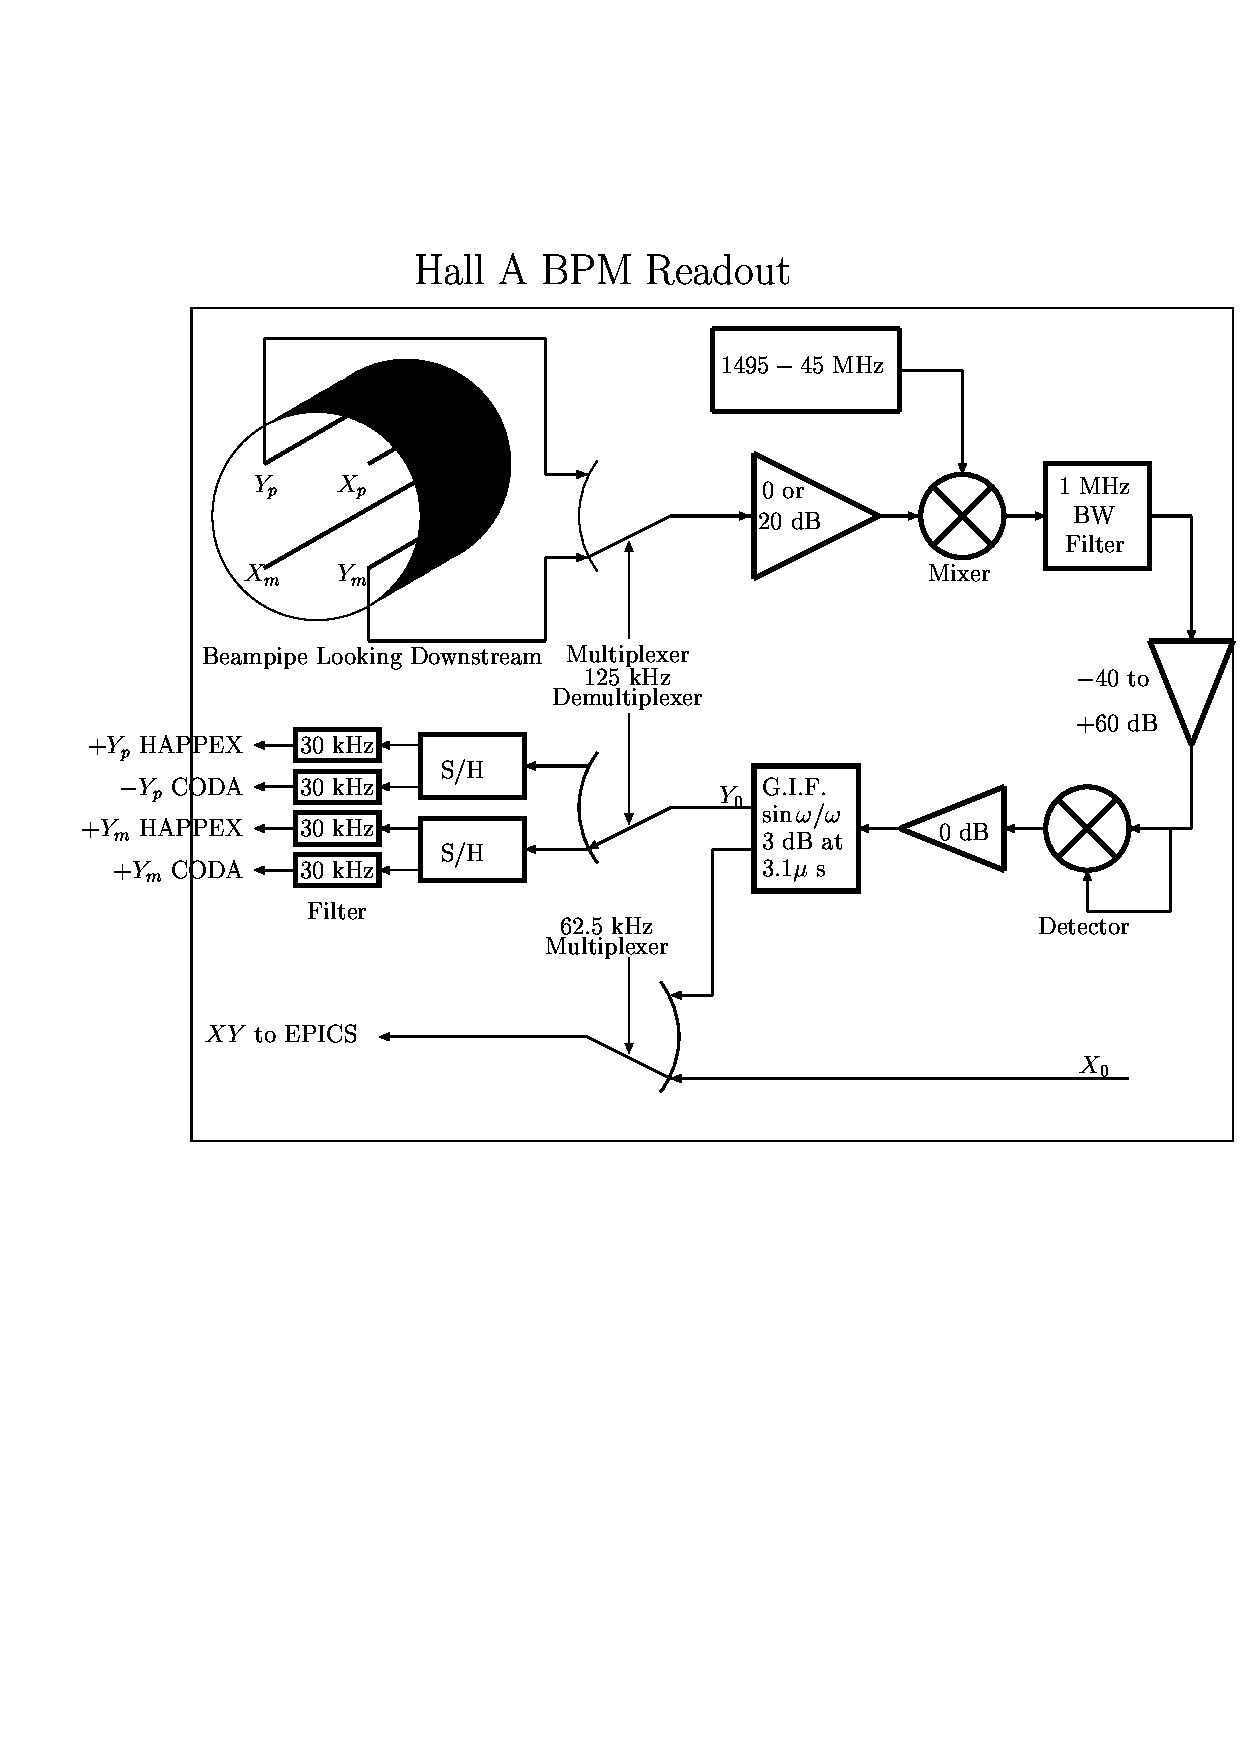
\includegraphics[angle=0,width=15cm]{BPM_fig}
{\linespread{1.}
\caption[Beamline: BPM Readout Electronics]{Schematic of the BPM readout
electronics}
\label{fig:bpmel}}
\end{center}
\end{figure}
}

1. The averaged position over 0.3 seconds is logged into the EPICS~\cite{EPICSwww} database (1 
Hz updating frequency) and injected into the datastream every 3-4 seconds, 
unsynchronized but with an orientative timestamp. From these values we can 
consider that we know the average position of the beam calculated in the EPICS 
coordinate system which is left handed.

2. Approximately once a shift (or more often if requested by the experimenters) 
a B-scope procedure ~\cite{bi:TP} can be performed using the same EPICS electronics 
which then gives the peak-to-peak variation of the beam.

3. Event-by-event information from the BPMs are recorded in the CODA datastream
from each of the 8 BPM antennas (2x4) from which the position of the beam can be 
reconstructed. However, these raw values belong to a parallel electronics chain 
whose constants have to be retrieved by calibrations to the EPICS or scanner 
data. 

\subsection{Beam Exit Channel}

After the target vacuum chamber, which was built by
the University of Virginia, there is an exit beam pipe which 
transfers the scattered beam onto the dump tunnel under vacuum. This exit beam 
pipe is made of a thin walled aluminum spiral corrugated pipe of welded 
construction. The largest diameter is 36 inches with a 0.164 inches wall 
thickness and the smallest diameter is 6 inches with a 0.042 inches wall 
thickness. The whole assembly is rather light (approximately 800 kg) and is 
supported by H shaped adjustable stands. To prevent possible linear collapse 
of the larger diameter sections under vacuum load, four aluminum channels of 
total cross-sectional area of 3'' are welded to its side. A vacuum of 
10$^{-5}$ Torr is maintained with a turbomolecular pump. The exit face of this 
pipe has a 12'' port and is connected to the diffuser with a Beryllium 
window.

}

\section{ Machine/Beamline protection system}
\label{sec:beam-fsd}

The MPS~\cite{MPScebaf} system is composed of the Fast Shutdown System (FSD), Beam Loss 
Monitor (BLM), and gun control system.

The FSD system is a network of permissive signals which terminate at the 
electron gun and chopper 1. The permissive to the gun and chopper
1 may be inhibited by any device connected to an FSD mode. Devices connected to the 
FSD system include vacuum valves, RF systems, Beam loss systems, beam current 
monitors, beam dumps, and particular to Hall A, the target motion mechanism 
and the raster (value and derivative).

The gun control system includes software program which monitors beam 
operating conditions and the state of the FSD and BLM systems. the program 
will warn the operators if a potential for beam damage exists. Potential for 
damage exists when running high average current beam, when FSD nodes are 
masked and when the beam power approaches the operating envelope limits for a 
specific beam dump.

\clearpage
\begin{safetyen}{10}{10}
\section{Safety Information}
\end{safetyen}
}
%
% Information for the ESAD
%

\begin{safetyen}{0}{0}

The beamline in the Hall provide the interface between the CEBAF accelerator
and the experimental hall.   All work on the beamline must be coordinated 
with both physics division and accelerator division; in order to ensure
safe and reliable transport of the electron beam to the dump.

\subsection{Hazards and Mitigations}

All magnets (dipoles, quadrupoles, sextupoles, beam correctors) and beam 
diagnostic devices (BPMs, scanners, Beam Loss Monitor, viewers) necessary for 
the transport of the beam are controlled by Machine Control Center (MCC) 
through EPICS~\cite{EPICSwww}, except for special elements which are addressed in the 
subsequent sections. The detailed safety operational procedures for the Hall 
A beamline should be essentially the same as the one for the CEBAF machine 
and beamline.\\ 

  
\noindent{}Personnel who need to work near or around the beamline should keep in mind the potential hazards:
\begin{itemize}
  \item Radiation ``Hot Spots'' - marked by ARM or RadCon personnel,
  \item Vacuum in the beam line tubes and other vessels,
  \item Thin windowed vacuum enclosers (e.g. the scattering chamber),
  \item Electric power hazards in vicinity of the magnets,
  \item Magnetic field hazards in vicinity of the magnets, and
  \item Conventional hazards (fall hazard, crane hazard etc.).
\end{itemize}

The most hazardous areas along the beamline are roped off it restrict access.   
In particule the scattering chamber, with it's large
volume and thin windows requires hearing protection once it has been evacuated.   
Signs are posted by radcon for any hot spots along the beamline and
radcon must be notified before work is done in a posted area.

Some magnets, as the M{\o}ller spectrometer elements, are covered with plastic
sheets for electric safety. Any access to these magnets requires
the ``Lock and Tag'' procedure~\cite{EHScebaf} and the appropriate training,
including the equipment-specific one. \\

\noindent{}Additional safety information is available in the following documents:
\begin{list}{--}{\setlength{\itemsep}{-0.15cm}}
  \item EH\&S Manual~\cite{EHScebaf};
  \item PSS Description Document~\cite{PSScebaf}
  \item Accelerator Operations Directive~\cite{AODcebaf};
\end{list}

\subsection{Responsible Personnel}

Since the beamline requires both accelerator and physics personnal to maintain
and operate and it is very important that both groups stay in contact that any 
work on the Hall A beamline is coordinated.

\begin{namestab}{tab:beam:personnel}{Beam line: authorized personnel}{%
   Beamline physics division and accelerator divison points-of-contact.}
  \namestabheader{Hall A Physicists}
  \DouglasHiginbotham{\em 1st Contact}
  \RobertMichaels{\em 2nd Contact}
  \namestabheader{Liaisons from Accelerator Division}
  \HariAreti{..to Physics}
  \YvesRoblin{..to Hall-A}
\end{namestab}
\end{safetyen}


\newpage
\section{ Beam Position Monitors}

To determine the position and the direction of the beam on the experimental 
target point, two Beam Position Monitors (BPMs) are located at distances 7.524 m 
(IPM1H03A) and 1.286 m (IPM1H03B) upstream of the target position. 
The BPMs consist of a 4-wire antenna array of open ended thin wire striplines 
tuned to the fundamental RF frequency of 1.497 GHz of the beam ~\cite{bi:bar90}. The 
standard difference-over-sum technique is then used ~\cite{bi:HW} to determine the 
relative position of the beam to within 100 microns for currents
above 1 $\mu $A. The absolute  position of the BPMs can be calibrated with respect to the 
scanners (superharps) which are located adjacent to each of the BPMs (IHA1H03A 
at 7.353 m and IHA1H03B at 1.122 m upstream of the target). The schematic of the 
readout electronics is shown in Figure ~\ref{fig:bpmel}. The
position information from the 
BPMs can be recorded in three different ways:

\begin{figure}
\begin{center}
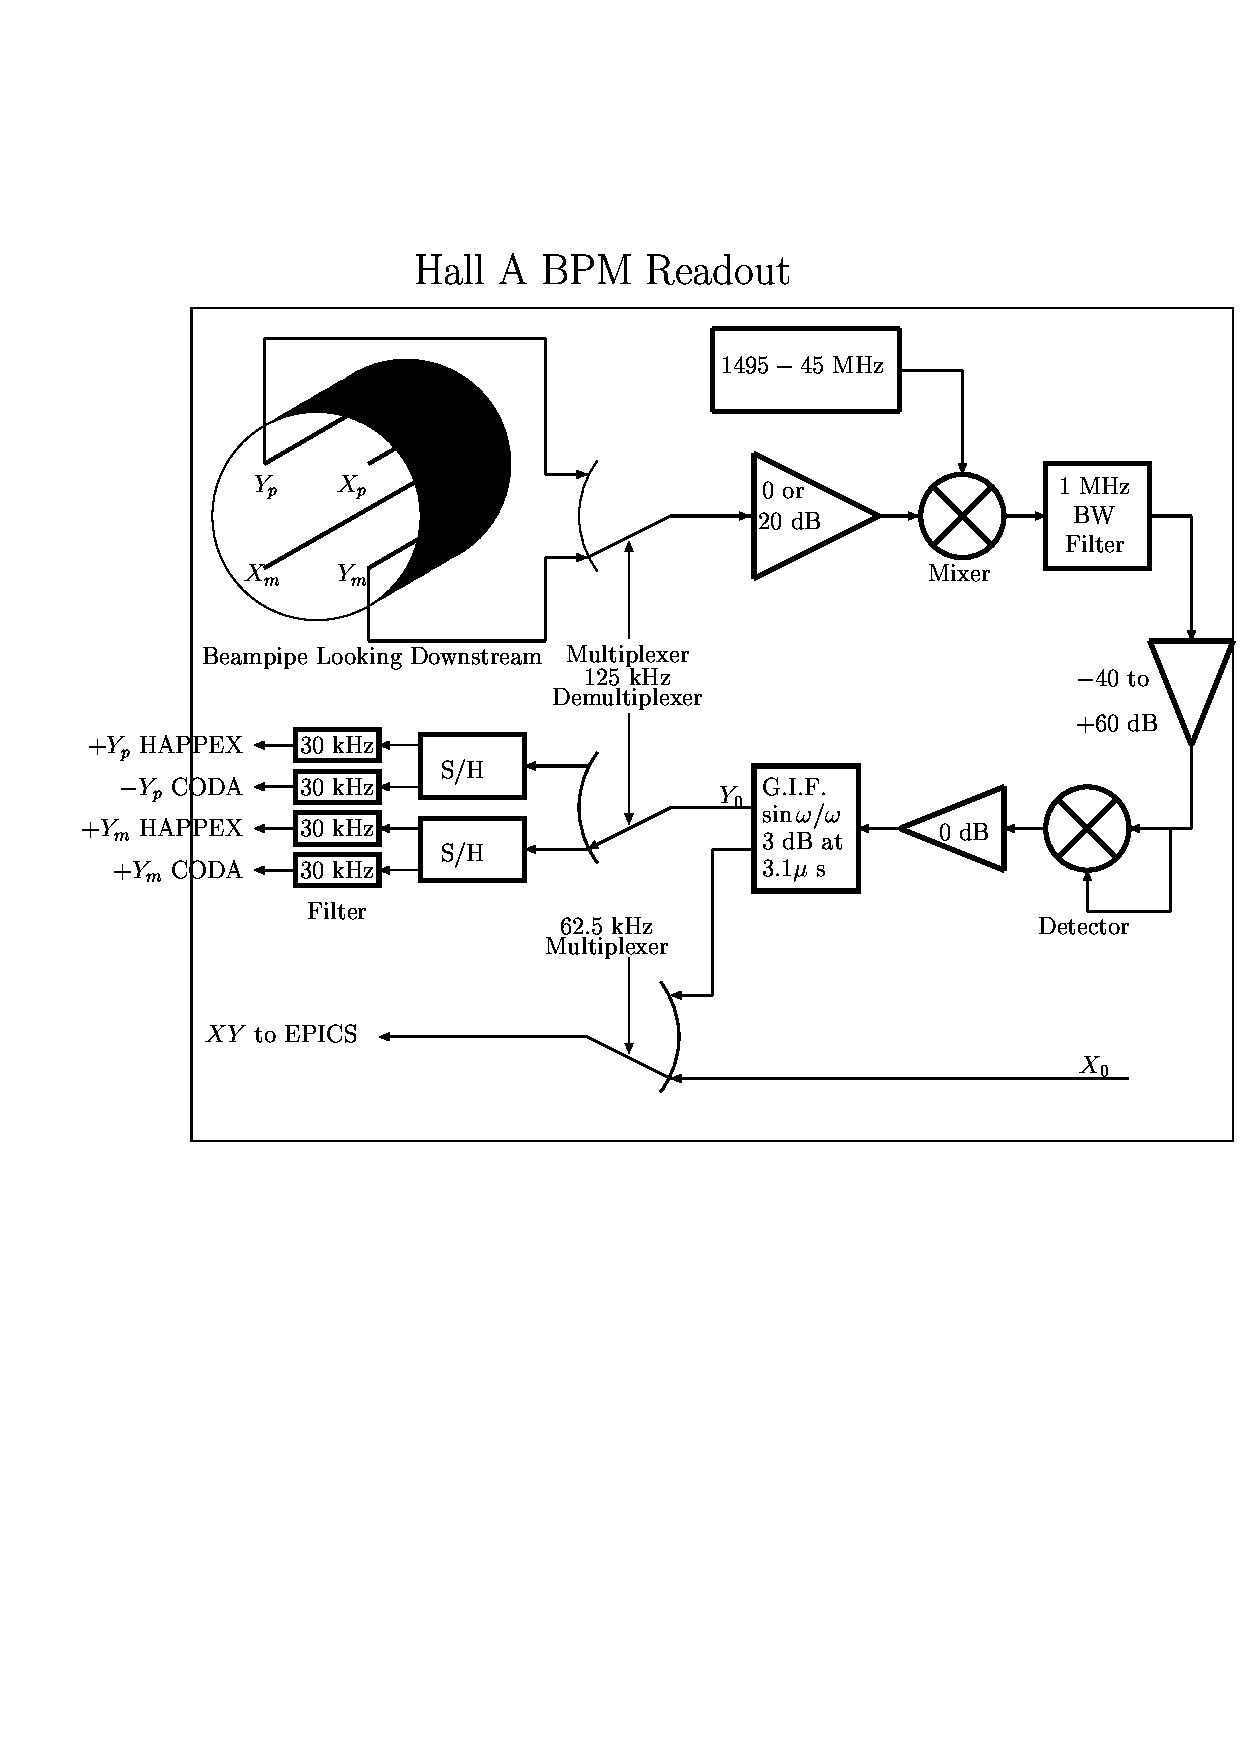
\includegraphics[angle=0,width=15cm]{BPM_fig}
{\linespread{1.}
\caption[Beamline: BPM Readout Electronics]{Schematic of the BPM readout
electronics}
\label{fig:bpmel}}
\end{center}
\end{figure}

\vskip 0.5cm

1. The averaged position over 0.3 seconds is logged into the EPICS database (1 
Hz updating frequency) and injected into the datastream every 3-4 seconds, 
unsynchronized but with an orientative timestamp. From these values we can 
consider that we know the average position of the beam calculated in the EPICS 
coordinate system which is left handed.

\vskip 0.5cm

2. Approximately once a shift (or more often if requested by the experimenters) 
a B-scope procedure ~\cite{bi:TP} can be performed using the same EPICS electronics 
which then gives the peak-to-peak variation of the beam.

\vskip 0.5cm

3. Event-by-event information from the BPMs are recorded in the CODA datastream
from each of the 8 BPM antennas (2x4) from which the position of the beam can be 
reconstructed. However, these raw values belong to a parallel electronics chain 
whose constants have to be retrieved by calibrations to the EPICS or scanner 
data. 


%\begin{thebibliography}{99}
%\bibitem{bi:bar90} W. Barry et al., CEBAF-PR-90-009 (1990).
%\bibitem{bi:HW} C. Hyde-Wright et al., Beam Position Studies for E93050 and priv. comm..
%\bibitem{bi:TP} T. Powers, priv.  comm.. 
%\end{thebibliography}
% ===========  CVS info
% $Header: /group/halla/analysis/cvs/tex/osp/src/beamline/bpms.tex,v 1.1 2003/06/05 17:28:32 gen Exp $
% $Id: bpms.tex,v 1.1 2003/06/05 17:28:32 gen Exp $
% $Author: gen $
% $Date: 2003/06/05 17:28:32 $
% $Name:  $
% $Locker:  $
% $Log: bpms.tex,v $
% Revision 1.1  2003/06/05 17:28:32  gen
% Initial revision
%

\newpage
\section[Beam Current Measurement]{Beam Current Measurement
\footnote{
  $CVS~revision~ $Id: bcm.tex,v 1.5 2003/12/13 06:23:37 gen Exp $ $
}
\footnote{Authors: A.Saha \email{saha@jlab.org}}
}

The Beam Current Monitor (BCM) is designed for stable, low noise, non-intercepting 
beam current measurements. It consists of an Unser monitor, two rf cavities, 
the electronics and a data acquisition system. The cavities and the Unser monitor 
are enclosed in a box to improve magnetic shielding and temperature stabilization.
The box is located 25 m upstream of the target. You can recognize it as a grey 
object on the stands, about 2 m downstream from where the beam enters the 
hall. 

The DC 200 down-converters and the Unser front end electronics are located in Hall 
A. The temperature controller, the Unser back end electronics and its calibration 
current source, cavity's RF unit (housing the RMS-to-DC converter board) and all 
multi-meters, VME crate and computers are located in Hall A control room.

\infolevone{
\subsection{ System Layout}

The schematic diagram of the BCM system is presented in
Fig.~\ref{fig:halla_bcm}.
\begin{figure}[htp]
\begin{center}
\includegraphics[angle=0,width=0.9\textwidth,clip]{habcm_r}
{\linespread{1.}
\caption[Beam Current Measurement: Schematic]{Schematic of the Hall A beam
current measurement system.}
\label{fig:halla_bcm}}
\end{center}
\end{figure}

The Unser monitor is a Parametric Current Transformer designed for non-destructive 
beam current measurement and providing an absolute reference. The monitor is 
calibrated by passing a known current through a wire inside the beam pipe and has a 
nominal output of 4 mV/$\mu $A. It requires extensive magnetic shielding and 
temperature stabilization to reduce noise and zero drift. As the Unser monitor's 
output signal drifts significantly on a time scale of several minutes, it cannot be 
used to continuously monitor the beam current. However, this drift is measured 
during the calibration runs (by taking a zero current reading) and removed in 
calibrating the cavities.  The more stable cavities are then used to determine the 
beam current and charge for each run. We also use the OLO2 Cavity Monitor and the 
Faraday Cup 2 at the Injector section to provide an absolute reference during 
calibration runs.

The two resonant rf cavity monitors on either side of the Unser Monitor are 
stainless steel cylindrical high Q ($\sim 3000$) waveguides which are tuned to the 
frequency of the beam (1.497 GHz) resulting in voltage levels at their   outputs 
which are proportional to the beam current. Each of the rf output signals from the 
two cavities are split into two parts. One part of the signal is  converted to 10 
kHz signals (by the ``downconverters'') and fed into an RMS-to-DC converter board 
consisting of a 50 kHz bandpass filter to  eliminate noise, amplified and split to 
two sets of outputs, which after further processing are recorded in the data 
stream. These two paths to the data stream (leading to the sampled and integrated
data ) will now be described. (The other part of the split signal is downconverted 
to 1 MHz signals and represents the old system (pre Jan 99). Only the HAPPEX 
collaboration presently uses these signals.)

For the sampled (or EPICS~\cite{EPICSwww} or Slow) data, one of the amplifier outputs is sent to a 
high precision digital AC voltmeter (HP 3458A). Each second this device provides 
a digital output which represents the  RMS average of the input signal during that 
second.  The resulting number is  proportional to the beam charge accumulated 
during the corresponding second (or, equivalently, the average  beam current  for 
that second). Signals from both cavity's multi-meters, as well as from the 
multi-meter connected to the Unser, are transported through GPIB ports to the HAC 
computer where they are recorded every 1 to 2 seconds via the data-logging process 
which is described in the calibration procedure. They are also sent through EPICS 
to CODA and the data stream where they are recorded at  quasi-regular intervals, 
typically every two to five  seconds.

For the integrated (or VTOF or Fast) data, the other amplifier output is sent to an 
RMS-to-DC converter which   produces  an analog DC  voltage  level. This level 
drives a Voltage-To-Frequency (VTOF) converter whose output frequency is  
proportional to the  input DC voltage level. These signals are then fed to Fastbus  
scalers and are finally injected into the data stream along  with the other scaler 
information.  These scalers simply accumulate during  the run, resulting  in a 
number which is proportional to the time integrated voltage level and therefore 
more accurately represents the true integral of the current and hence the total 
beam charge. The regular RMS to DC output is linear for currents
from about 5 $\mu$A to somewhere well above 200 $\mu$A.
 Since it is non-linear at the lower 
currents, we have introduced a set of amplifiers with differing gains (x3 and x10) 
allowing the non-linear region to be extended to lower currents at the expense of 
saturation at the very high currents. Hence there are 3 signals coming 
from each BCM (Upx1, Upx3, Upx10, Dnx1, Dnx3, Dnx10). All 6 signals are fed 
to scaler inputs of each spectrometer (E-arm and H-arm) . Hence we have a 
redundancy of 12 scaler outputs for determining the charge during a run. During 
calibration runs we calibrate each of these scaler outputs.   
}

\begin{safetyen}{10}{10}
\subsection{ Authorized Personnel}
\end{safetyen}

All Hall A members are authorized to take BCM calibration data using the Standard 
Non-Invasive Hall A BCM Calibration Procedure. The extended calibration procedures 
involving the Faraday Cup 2 and the OLO2 monitor at the Injector are presently 
performed by A. Saha. 

\vskip 0.2cm

The Accelerator AES group performs the maintenance of the BCM monitors. These 
include:

\begin{tabular}{l l}
1. The Unser calibration. & Every 3 months \\
2. Resonant Cavities Tuning. & Every Downtime \\
3. Multi-meters Autocalibration. & Every Downtime \\
4. Connectors Cleaning. &  Every year \\
5. Unser Keithley Current Source. & Calibration Yearly \\
6. Digital Multi-meters HP3458A and HP 34401A. & Calibration Yearly\\   
\end{tabular}

System Contacts are shown in Table~\ref{tab:BCM:personnel}.
\begin{namestab}{tab:BCM:personnel}{BCM: authorized personnel}{%
   Beam Current Monitor: authorized personnel}
  \ArunSaha{\em Contact}
  \JohnMusson{Accel. expert}
\end{namestab}
%Jean-Claude Denard -x 7555




% ===========  CVS info
% $Header: /group/halla/analysis/cvs/tex/osp/src/beamline/bcm.tex,v 1.5 2003/12/13 06:23:37 gen Exp $
% $Id: bcm.tex,v 1.5 2003/12/13 06:23:37 gen Exp $
% $Author: gen $
% $Date: 2003/12/13 06:23:37 $
% $Name:  $
% $Locker:  $
% $Log: bcm.tex,v $
% Revision 1.5  2003/12/13 06:23:37  gen
% Septum added. Name tables. Polishing
%
% Revision 1.4  2003/12/05 05:48:30  gen
% Polishing
%
% Revision 1.3  2003/06/06 15:19:02  gen
% Revision printout changed
%
% Revision 1.2  2003/06/05 23:29:59  gen
% Revision ID is printed in TeX
%
% Revision 1.1.1.1  2003/06/05 17:28:32  gen
% Imported from /home/gen/tex/OSP
%
%  Revision parameters to appear on the output

\newpage
\section[Fast Raster]{Fast Raster
\footnote{Authors: R.~Michaels \email{rom@jlab.org}}
}


The beam is rastered on target with an amplitude of
several millimeters at 25 kHz to prevent overheating.  
The raster is a set of four of air-core dipoles located
approximately 23 m upstream of the target. 
Two dipoles are for horizontal (X) motion and
another two for vertical (Y).  During the 6 GeV era
there was only one pair of X and Y, but we have doubled
the raster to account for the energy increase to 11 GeV.
The arrangement along the beamline along the 
direction of the beam will be XXYY.

For a typical 40A current in the raster coils, the
deflection by one pair (e.g. the X direction) of coils, 
in radians, is $\theta = 1.94 \times 10^{-3}/ E$
where $E$ is the electron's energy in GeV.
For example, at $E = 6$ GeV, a 0.32 mrad deflection is achieved.
Projected onto the target (about 21 m away) this is a $\pm$ 6.8 mm
excursion {\it if} there were no other magnetic fields 
between the raster and the target; however, there are quadrupoles
which change this depending on the beam tune.

Since 2003 we've used the triangle-wave 
raster pattern designed by Chen Yan.  
This achieves a very uniform rectangular
density distribution of beam on the target 
by moving the beam with a time-varying dipole
magnetic field whose waveform is triangular
with very little dwell time at the peaks.  
The electronics design is an ``H-bridge''
in which switches are opened and closed 
at 25 kHz, to switch between two directions 
of current (100 A peak-to-peak) 
through the raster coils.

Three new features during the 12-GeV era are 
1) the driver of the H-bridge electronics is now
an Agilent model 33522A waveform generator; and
2) The two X are synchronized with each other, and
the two Y are synchronized.  This makes the kicks
add and allows us to accomodate the higher energy
of the beam; and 3) The entire raster can
be synchronized to an external 10 MHz wavetrain
supplied by the polarized injector electronics.
This makes the nominal 25 kHz an exact multiple of
the helicity-flip rate, which achieves a cancellation
of raster noise, important for parity-violation 
experiments only.
The syncrhronization of the pairs of X and Y are
accurate to within a few nsec.

For most users, these three new features will not be
noticeable and the raster will appear to function
the same as during the 6 GeV running.
A user can view the 
status of the raster in the
EPICS overview screen called ``General Accelerator
Parameters'' where the set-point for the radius amplitude
and the readback of the peak-current in the raster are displayed.

Control of the raster is done by first asking the MCC
operators to set up the raster for a particular size
typically 2 mm square.
The control software assumes a field-free region between
the raster and the target, so it is only approximately
correct because there are several quadrupoles in this region.
It is important to check the raster spot size and
make adjustments if necessary.  The adjustment is made
by asking MCC to change the size and noting the 
linear relationship between what their software says
the size is and the actual size.
Relatively small independent adjustments to the 
gains on the X and the Y raster
coils are available in the middle room of the hall A
counting room using the ``PGA Controller'' knobs;
however, it is not recommended to touch these.
Near these knobs is also located an oscilloscope X-Y trace
of the current in the raster.  A fast shutdown (FSD) shuts
the beam down within 0.1 msec if the raster fails, thus
affording some protection of the target.

{\it NOTE:  If you are unsure of the status of the raster,
measure the spot size with very low current ($\le 2 \mu$A) or with
the target out of the beam.}  It would be a mistake
to check the beam spot size with high current on target; by
the time you check it, the target may already be destroyed.
The rastered beam spot on target can be checked with
plots in the ROOT analyzer or by 
using the stand alone code called \mycomp{spot},
also called \mycomp{raster}.
For more details on usage, type \mycomp{spot -h} (help)
on the ADAQ computers.

Regarding the BPM measurements, it should be noted that 
the stripline BPMs displayed by \mycomp{spot} have a high-frequency 
cutoff of approximately 30 kHz.  Since the raster frequency is 25 kHz
the plot of the amplitude distribution shows spikes at the 
limits of the orbit, instead of a flat distribution.  The scale
factor between what is seen in \mycomp{spot} and the real width of the beam
is $\sim 1.5$, i.e. the beam is 1.5 times bigger than the naive
reading of the \mycomp{spot} distribution.



\newpage
% Updated Comments Dec. 2
\infolevone{
\chapter[Arc Energy Measurement]{Arc Energy Measurement
\footnote{Authors: D. Higinbotham \email{doug@jlab.org}}
}
}

\infoleveqnull{
\section{Arc Energy Measurement}
\subsection{Overview}
In order to determine the integral field of the eight dipoles that lead to Hall A, and 
in turn determine the beam energy, a nineth dipole wired in series with the rest is 
located in a special shed near the hall A counting house.
}

\infolevone{
The ARC energy measurement is under EPICS~\cite{EPICSwww} control through 
a MEDM~\cite{MEDMwww} display. Two
independent control systems are used: the beam bend angle measurement through
the arc ("scanners") and the field integral of
the arc ("integral"). To measure the energy: 

\begin{itemize}
\item perform several angle measurements 
\item perform an integral measurement 
\item analyze the integral measurement and note the value of the arc field 
integral 
\item analyze the angle measurements, average the results (proposed by the 
software),
then ask for the energy calculation, enter the above arc field integral and
you will get the beam energy computed from the average angle. 
\end{itemize}

\section{Summary of ARC operations }

Six scanners of the same type, called ``ARC scanner'' and labelled
from scanner \#1 to \#6, are installed on the Hall-A beamline. Scanners \#1
to \#4 are used for the ARC energy measurement and they are located on the Hall-A
arc: \#1 [1HA1C07A] and \#2 [1HA1C07B] just upstream of the arc, in the BSY, and 
\#3 
[1HA1C18A] and \#4 [1HA1C18B] in the Hall-A
tunnel, just upstream the Compton polarimeter. Scanners \#5 [1HA1H03A] and \#6 
[1HA1H03B] 
are located
between the Moller and the target to control the beam geometry on the target
and their use will not be discussed here. 

Procedure for running a harp scan is described elsewhere\footnote{
Harp scan procedure \url{http://hallaweb.jlab.org/equipment/beam/harp_halla/harp.html}.}

Each scanner has a motor/ball-screw/shaft-encoder/vacuum-penetrator system moving
accurately a set of 3 tungsten wires through the beam. Each time a wire crosses
the beam a PMT located a few meters downstream records a signal due to the 
electromagnetic
shower induced by the beam in the wire. Both forward and backward passes are
recorded. The motion is a horizontal translation and, for a forward pass: 

-the translation is from beam left to beam right, 

-the two first wire crossing the beam are at 45deg from the vertical, 

-the third wire, which is the only important for the ARC energy measurement,
is vertical. 

Recording, during the scan, the scanner position and the PMT output voltage
allows us to determine the beam position at each scanner location. Then, using
calibration data not detailed here, we deduce the net beam bend angle through
the arc. This result measured in dispersive arc tuning, along with the field
integral of the arc dipoles, provides an accurate determination of the beam
energy. 

\vspace{0.3cm}

\section{Summary of field integral }

The purpose is to measure absolutely the straight field integral of a 
"BA"
3m long dipole, called the "9th dipole" and located in the
"Dipole Shed". It is of the same type as the 8 arc dipoles
and is powered in series with them. 

The ARC integral setup is basically made of a 3m long plate (the 
"probe")
which is able to move inside the 9th dipole gap along the beam axis and carrying 
two
field measurement devices: a pair of pick-up coils connected in series and a
set of NMR probes. The coils are on both ends of the probe and the NMRs close
to the center. 

-at the "upstream" probe position, the 
"downstream"
coil is close to the dipole center, the "upstream" is outside
the dipole and the NMRs at one end of the dipole: 

Door$<-$-- ....................$<-$-------DIPOLE-----$--->$ 

.............$<-$-------PROBE------$--->$ 

-at the "central" probe position, each coil is at one end
of the 3m long dipole and the NMRs close to the dipole center: 

Door$<-$-- ...................$<-$-------DIPOLE-----$--->$ 

..................................$<-$-------PROBE------$--->$ 

-at the "downstream" probe position, the 
"upstream"
coil is close to the dipole center, the "downstream" is outside
the dipole and the NMRs at one end of the dipole: 

Door$<-$-- ...................$<-$-------DIPOLE-----$--->$ 

....................................................$<-$-------PROBE------$--->$ 

We call upstream the position where the probe is the closest to the shed access
door. Among the 3 above positions, the only one where the NMR can lock on the 
dipole
field is the central one as in the extreme position of the probe, the field 
homogeneity
is not sufficient. The probe position is controlled by a linear encoder. The
Z axis refers to the "beam" direction, increasing from upstream
to downstream. We use three kinds of "Z": 

-Zm to locate a point inside the magnet. The dipole center is at Zm=0 and the
yoke ends at +-1500.mm 

-Zp to locate a point inside the probe. The probe center is at Zp=0. Each of
the 4 NMR probes has a Zp given in the file "magnet.dir".
At a temperature of 21C, the coils are at Zp=+-1519.815mm (from magnet.dir) 

-Zd to refer to a displacement of the probe w.r.t. the dipole. Zd=0 refers to
the upstream (home) position of the probe. The integral measurement is performed
from Zd=0.000mm (1st PDI trigger) to Zd=3199.000mm (last PDI trigger), for forward
pass. Zd is given by the display (at the top of the rack) or by the master screen
("OUT"). 

The relationship between Zm, Zp and Zd is: 

Zd-Zm+Zp=C 

where C is a constant given in magnet.dir (C=1604.000 nomin.). Example of use:
to have the probe center at the dipole center, one must set Zd=1604.000mm (set
Zm=0 and Zp=0 in the above formula, and solve for Zd) 

The integral measurement sequence is the following: 

-from the current position (a priori arbitrary) move the probe upstream, up
to a limit (optic) switch. 

-move downstream by a few mm to cross the encoder index (encoder initialization) 

-move to the central position to measure the central field by NMR, the system
checks if the NMR locks and if the reading is stable, it will be the 
"before"
field 

-move back to upstream position 

-move to downstream position while integrating the flux through the coil system,
this measurement will be called the "forward" integral (duration
\( \sim  \) 7s) 

-move back to upstream position while integrating the flux through the coil
system, this measurement will be called the "backward" integral
(duration \( \sim  \)7s) 

-move to the central position to measure the central field by NMR, the system
checks if the NMR locks and if the reading is stable, it will be the 
"after"
field. 

In addition to the central field, 4 probe temperatures, a local excitation current
measurement, the setting of the dipoles P.S, the readback of the dipoles P.S
and the probe position at NMR measurement time are recorded 
"before"
and "after". 

To perform an integral field measurement: 

1-check if the system works (see "details on integral system 
check"
below) 

2-run the above integral sequence (see "details on integral run"
below) 

3-fix the error(s) if any (see "details on integral errors"
below) 

4-save the data in a file (see "details on integral data save"
below) 

5-analyze the data  


\section{Details on integral run }

To run the integral measurement sequence, call the 
\mycomp{arc\_integral.adl}
medm screen, then: 

-push "start" to start the full sequence 

-look at the results displayed: 

-after the "before" NMR measurement: the 
"before"
data set 

-after the "forward" integral pass: the forward velocity profile
and the forward voltage-after-gain profile 

-after the "backward" integral pass: the backward velocity
profile and the backward voltage-after-gain profile 

-after the "after" NMR measurement: the 
"after"
data set 

-if "BAD NMR" or "PDI saturation" flags
are set, or if something is obviously wrong in the data or plots, call expert. 

-data are ready to be saved (see "Details on integral data save"
below) 


\section{Details on temperatures }

The AC system of the shed is made of two cooling units, a heating unit and a
controller connected to two temperature sensors : one located in the shed and
one located in the BSY. This system is programmed in such a way that the 
temperature
of the shed follows the BSY temperature within +-2C. The BSY temperature can
be anywhere in the 18C to 35C range, regardless of the season. The BSY 
temperature
and the shed temperature are given (in F) by a display panel located close to
the workstation, on the wall. The AC system can be set in manual control by
turning from "auto" to "manual" a set of
switches controlling the cooling units and the heater unit. These switch boxes
are located on the shed wall. If the shed temperature is above 34.4C (94F),
call the crew chief (the electronics can be damaged) and cool down the shed in manual
AC mode. The 4 temperature sensors of the probe are labelled Tx+z+, Tx+z-, Tx-z+,
Tx-z- depending on their position w.r.t. the frame. 

Both "x+" sensors are on the probe edge which is inside the
dipole gap and both "x-" sensors on the opposite edge which
is outside the dipole gap. Both "z-" sensors are at 1/4 of
the long dimension of the probe and both z+ at 3/4 of this length. The average
of the 4 temperatures is used by the analysis program to correct the coil distance
from the thermal expansion of the probe, so it is important to make sure that
the 4 sensors are working well. The user can just make sure that the temperatures
displayed in \mycomp{arc-master.adl} or recorded in 
\mycomp{arc-integral.adl}
are realistic. In \mycomp{arc-integral.adl} they are given in the
order: Tx+z-, Tx+z+, Tx-z-, Tx-z+ Tx-z- and Tx-z+ should be close to the shed
temperature. Tx+z- and Tx+z+ depend on the probe position, as the gap (iron
yoke) is warmer than the shed and the dipole coil (at both ends of the dipole)
is warmer than the iron yoke. For a probe in a central position for more than
about one hour, the Tx+z- and Tx+z+ sensors should give the yoke temperature,
i.e the shed temperature plus 0. to 5.C, depending on the current, LCW temperature
and the magnet/shed temperature history. The 4 temperatures are also displayed
inside the shed, on the electronics rack. These values are digitized by separate
ADCs, so they may differ from the remote values by \( \sim  \)0.1C. 
}

\begin{safetyen}{10}{10}
\infolevone{\section{Shed access and safety }}

Due to the the dipole magnet and motion system, the access to the shed is limited to authorized
persons which are listed in the ESAD and listed below. To be added to the list, 
contact Douglas Higinbotham.
The standard
operation mode of the integral measurement setup is the remote mode, through
the network, from the counting house.
\end{safetyen}

\begin{safetyen}{10}{10}
\infolevone{\section{List of Authorized Personnel for Shed Access}}
\infoleveqnull{\subsection{List of Authorized Personnel for Shed Access}}
\end{safetyen}
\begin{namestab}{tab:arc:personnel}{Arc Energy Measurement: authorized personnel}{%
                 Arc Energy Measurement: authorized personnel}
  \namestabheader{Hall A Personnel}
  \DouglasHiginbotham{\em Contact}
  \namestabheader{Accelerator Personnel}
  \MichaelTiefenback{}
  \YvesRoblin{}
  \RickGonzales{}
  \BillMerz{}
  \MarkAugustine{}
  \HariAreti{}
  \PeteFrancis{}
  \ScottHiggins{}
  \DavidSeidman{}
  \RonLauze{}
  \TonyDay{}
  \ChristopherCurtis{Alignment group}
  \namestabheader{CEA - Saclay experts}
  \PascalVernin{}
  \ChristianVeyssiere{}
  \FrancoisGougnaud{}
  \JacquesMarroncle{}
\end{namestab}



\newpage
\infolevone{
\chapter[Target Chamber]{Target Chamber
\label{sec:target_chamb}
\footnote{
  $CVS~revision~ $Id: tgtcham.tex,v 1.11 2005/04/04 22:27:25 gen Exp $ $
}
\footnote{Authors: ?? \email{??@jlab.org}}
}

The cryo-targets and the waterfall targets 
(see Sec.~\ref{sec:targets-overv}) 
are contained in a special target chamber which is a large 
evacuated  multistaged can. So far, three chambers have been designed:
\begin{list}{\arabic{enumi}.~}{\usecounter{enumi}\setlength{\itemsep}{-0.15cm}}
  \item a chamber used up to 2003;
  \item a chamber designed for use with septum magnets, starting in 2003;
  \item a chamber designed for use with the BigBite spectrometer.
%\footnote{
%        No yet manufactured by Dec,2003.}.
\end{list}

Here, chamber 1 is described. Chambers 2 and 3 are only different in 
size and slightly in shape. The safety considerations fully apply to chambers 2 and 3.
The chamber was designed to isolate the beam line vacuum from  each
HRS so that each HRS could rotate
around the target without vacuum coupling and without jeopardizing
certain desired kinematic and acceptance  specifications of 
both high resolution spectrometers
needed for approved experiments.  It  was also designed to simultaneously
 contain a liquid or gas target and an array of water cooled thin
 metallic foils, both remotely controlled and also be adaptable for
the waterfall target. The desired kinematic specifications that were
 considered included momentum and energy resolution in both arms,
 angular range of spectrometers, angular acceptance, and luminosity.
The chamber vacuum is isolated from the  HRS by using thin aluminum foils. 

The target chamber is designed so that
each spectrometer will have continuous coverage in the standard tune from
$\theta_{min}=$12.54$^\circ$ to $\theta_{max}=$165$^\circ$.
The aluminum window is 6~$in$ high and 0.016~$in$ thick made of 5052 H34 aluminum foil.
The foil forms regularly spaced vertical ridges when
placed under load. The window had an inter-ridge
spacing of 3 inches.
If the window is treated as a collection
of smaller rectangular windows which have the full vertical height
of 6 inches and the inter-ridge spacing as a width,
then stress formulas predict that the 0.016 $in$
material would reach ultimate stress at a pressure higher than 35 PSID
(for both over-pressure and under-pressure). 
There is a gate valve between the 
scattering chamber and the beam entrance (exit) 
pipe. Both 
valves will be closed automatically in the
event that the chamber vacuum begins to rise and an FSD will be caused
( this is done via a relay output of the scattering
chamber vacuum gauge). If either valve is closed an FSD will result.

The target chamber is supported by a 24 $in$ diameter pivot post
secured in concrete, rising about 93.6 $in$ above the Hall A cement floor.
The Hall A target chamber
consists of an aluminum middle ring, a stainless steel base ring,
each with a 41.0 $in$ inner diameter,
and a stainless steel cylindrical top hat with 40 $in$ inner diameter
to enclose the cryotarget and secure the cryogenic connections.

When the scattering chamber is under vacuum, there is a potential
danger of window rupture.
The loud noise from the rupture could hurt
one's ears if not protected. Therefore when the chamber is under vacuum,
protective covers are put on if possible. These must be taken off
for data taking. For restricted access, the protective cover is required
to be on when the chamber is under vacuum. Before switching from controlled
access to restricted access, the protective cover is required to be installed.
Anytime that the scattering chamber
is under vacuum, the pivot area is enclosed in a rope or tape barrier
and a warning sign is posted.
Hearing protection is required in the enclosed area.

\infolevone{
	The aluminum ring with an outer diameter of 45.0 $in$ and
wall thickness 2.0 $in$  is necessary for a sturdy support structure and
to permit machining of the outside surface to accommodate
the flanges for fixed and sliding seals mounted on
opposite sides of the ring that vacuum connect the chamber to each HRS.
The height of the aluminum ring shown is 36.0 $in$, which is
designed to accommodate the mounting flanges.
The stainless steel base ring 
is 11.50 $in$ in height with
one pump-out 6 $in$ diameter port  and with
seven 4 $in$ viewing and electrical feed-through ports.
The base ring will also contain support mechanisms for the solid
target ladder assembly, a rotisserie for collimating slits, radiators, and
magnetic
fingers for
removing the solid target vacuum-lock can. The total height of the top
ring, middle ring, and
base ring is 93.81 $in$. This length is partly determined by our desire to
include with the cryogenic extended target a solid target vertical ladder
secured in an inverted hat through a hole in the base of the chamber.

	The base ring includes an end plate through which the
inverted hat will be adapted to fit into the large vertical pipe serving
as the pivot post for the Hall A spectrometers.

	The stainless steel cylindrical top hat  has
40.0 $in$ inner diameter, and is 0.375 $in$ thick and
46.31 $in$ high , which is necessary to permit the
cryotarget to be withdrawn and to make space available to expose the solid
targets to the electron beam.

   The 200 $\mu$A electron beam, focused to a $\sim$\(0.1\, mm\times
0.1\) mm spot and rastered $\pm$5 mm horizontally or vertically on the
target, enters through a oval hole in the middle ring which
is 2.06 $in$ wide and exits through a 1.81 $in$ hole connected to the
exit pipe.
}

\infolevone{
\section{Target Chamber - Spectrometer Coupling}

   The aluminum middle ring will support a flange on each side for each high
resolution spectrometer. Four flanges will be available: Two flanges will
contain a 6 $in$ window opening which will be covered with a thin foil
(e.g., 10 mil aluminum) .
These two flanges will be used for experiments utilizing
extended  targets that do not require optimum momentum resolution.
The other two flanges will have two fixed ports (with a 8 $in$ $\times$ 6 $in$
opening)
which will be mainly used for calibration of the spectrometers . Fixed ports are
centered at 16.11 $^\circ$ and
45 $^\circ$ for one flange and at 16.11 $^\circ$ and 90 $^\circ$ for the second
flange.

   For a point beam on target a vertical opening in the walls of the chamber
of height 57.15 cm x 0.065 x 2 = 7.43 cm is required so that the scattered
beam is within the full acceptance of the spectrometer.
If the beam is rastered on target $\pm$0.5 cm in the vertical direction,
then the opening in the outer side of the chamber must be at least 8.5 cm for
full acceptance.

From consideration of the angular range of the spectrometers in the standard
tune, the scattered beam acceptance envelope, the effects of an
extended gas target on acceptance,
and the effects of a rastered beam $\pm$ 5 mm on acceptance,
the target chamber requires a window of at least 8.5 cm
high in the aluminum ring extending from 6.33 $^\circ$ (2.48 in) from the
beam exit point to 8.83 $^\circ$ (3.47 in) from the beam entrance point on one
side and a similar window on the other side of the beam.
For future considerations (e.g., using a third arm or sliding seal) the
width of the window on the middle ring was actually constructed
to be 17.78 cm (7 $in$).

\section{Stress Analysis of the Middle Ring}

Since the middle ring has an extensive cut across the midplane on both sides as
well as
entrance and exit holes and loaded with about 25,000 lbs, calculations of the
stresses
 and deformation of  the
midplane support area of the middle ring and deflection of the window opening
were made using the finite element analysis code ANSYS . The work was conducted
by a graduate student in the Department of Civil Engineering at the
University of
Virginia and a REU student.  A scaled down model of the middle ring was
constructed and then tested by applying forces to it using the Materials Testing
Service of the Department of Transportation at the University. ANSYS was first
checked by comparing calculations of the test model deflections to the actual
data. Agreement was  within $\pm$10\%. Results of ANSYS for the target
chamber showed that the maximum deflection of the opening of the window in the
middle ring varied from 0.007 $in$ to 0.015 $in$ depending on how the
middle ring
was loaded. This was decided to be a safe limit. In the final design, several
movable
7 $in$ long, 2 $in$ diameter aluminum support rods are placed in the
window for added support. In addition, flanges defining the ports and
coupling to
the spectrometers can be added, giving additional support to the middle ring.
Compressional stresses, calculated using ANSYS assuming the middle ring was
attached to the
top hat and loaded with 25,000 lbs, were less than 3000 psi 
almost everywhere.
However, stresses over small areas rose to levels 6000 psi near the entrance
and exit holes. These calculations indicated that we did not exceed the safety
limit of 15,000 psi for aluminum. A simple model calculation shown in Appendix
A  gives the result 1434 psi, which represents some average value over the
midplane
contact area.

\section{Vacuum Pumping System}

The vacuum in the target chamber is maintained by an Alcatel ( 880 l/s)
 turbomolecular vacuum pump. The pump is connected to a 6 $in$ port in the
stainless steel ring between 130
 $^\circ \le \theta_p \le 180 ^\circ$. The vacuum pump is
fastened to a horizontal pipe connected to the chamber. The vacuum pressure in
the chamber is about $10^{-5}$ mm. An additional Alcatel pump connected
to an 8 $in$ port should be added to obtain lower vacuum. Both
pumps may be isolated
from the target chamber using gate valves which are remotely operated
from the vacuum control rack and interlocked to the FSD system.


A 2 $in$ all metal gate valve is located between the entrance flange to the
chamber and the beam profile monitor.   
 An additional gate valve is located 2 m downstream of the
 target chamber to isolate the chamber from the exit beam pipe.
}
\begin{safetyen}{10}{15}
\section{Safety Assessment}
\end{safetyen}

The scattering chamber is typically a low maintenance item but it is a vacuum
system and hence problems may occur. The day to day operations of the cryogenic
targets are managed by the Hall A Staff while major maintenance operations are
handled by the Cryogenic Target Group (Physics Division). Occasionally the
cryogenic targets experience difficulties due to failures of the End Station
Refrigerator which supplies the coolant. In these cases the Cryogenics Group
of the Accelerator Division should be contacted.

\noindent{}The target chamber may pose several hazards:

\begin{list}{\arabic{enumi}.~}{\usecounter{enumi}\setlength{\itemsep}{-0.15cm}}
  \item {\bf Rupture of vacuum windows}. This hazard is mitigated by
        lexan guards on the vacuum windows, installed by the hall technicians
        either at the beginning of a ``restricted access'' period 
        %(see Sec.\ref{sec:Access}),
        or during ``control access'', in case an access to the target chamber area is needed.
        Installation and removal of the guards is included in the technician's checklists.
        When the chamber is under vacuum, it is mandatory to use ear protection in the chamber
        vicinity. The appropriate signs must be installed by the technicians. 

  \item {\bf Induced radioactivity}. The RADCON surveyor measures the level of induced
        radiation as a part of the general survey and may declare the target area 
        as ``High Radiation Area'', installing a rope protection around\cite{RWIcebaf}. 

\end{list}

Some other safety issues are discussed in the cryo-target chapter 
(see Sec.~\ref{sec:target-cryo-safety}).
%and also in the polarized target chapter (see Sec.~\ref{sec:target-he3-general}).

\begin{safetyen}{10}{15}
\section[Authorized  Personnel]{Authorized  Personnel}
\end{safetyen}

\begin{namestab}{tab:targ_chamb:personnel}{Target chamber: authorized personnel}{%
      Target chamber: authorized personnel. ``W.B.'' stands for the white board 
      in the counting house.}
  \TechonCall{\em Contact}
  \JessieButler{}
  \DaveMeekins{Target group}
  \JianPingChen{}
\end{namestab}
}

\newpage
\infolevone{\chapter[M{\o}ller Polarimeter]{M{\o}ller Polarimeter}
\setcounter{subsection}{0}}
\infoleveqnull{\section[M{\o}ller Polarimeter]{M{\o}ller Polarimeter}}

The Hall A beam line is equipped with a M{\o}ller 
polarimeter
whose purpose is 
to measure the polarization of the electron beam delivered to the hall. 

\begin{safetyen}{0}{0}

The M{\o}ller Polarimeter system has under gone a major upgrade and an Operational Safety Proceedure (OSP)
is being written and must be reviewed before its use.

\subsection{Hazards and Mitigations}

The hazards and mitigations for this system can be found in the OSP at the end of this document. 

%\infolevone{
%Safety checklist item for this device, located at the end of the beamline section, is solely to ensure
%the beam can be tranported safetly past this system prior to it's recommisioning.
%}

\subsection{Responsible Personnel}
\label{sec:moller-pers}

This list of system experts provided in case there is any question as to the status of system.

\begin{table}[h]
\begin{center}
\begin{tabular}{|ll|l|l|l|l|r|} \hline
  \multicolumn{2}{|c|}{Name} & Dept. & \multicolumn{2}{c|}{Telephone} & 
  \multicolumn{1}{c|}{e-mail} & Comment \\ 
  \cline{4-5}
   &  &   & JLab & Pager &  & \\ 
\hline
 Javier       & Gomez           & JLab    & 7498 & 7498 & gomez@jlab.org    & Primary contact     \\ 
 Oleksandr    & Glamazdin       & Kharkov & 5441 & 5441 & glamazdi@jlab.org &  \\ 
 Viktor       & Gorbenko        & Kharkov & 5441 &   -  & gorbenko@jlab.org &  \\ 
 Roman        & Pomatsalyuk     & Kharkov & 5395 & 0001 & romanip@jlab.org  &  \\ 
\hline
\end{tabular}
\end{center}
\caption[Moller Polarimeter: authorized personnel]{
   The listed name are those who are considered system experts of the Moller Polarimeter and should be contacted
   if there is any question as to the status of the system.
}
\label{tab:moller:personnel}
\end{table}
\end{safetyen}


\newpage
}
% Compton Polarimeter
\infolevone{\chapter[Compton Polarimeter]{Compton Polarimeter}
\label{sec:compton}
\footnote{Author: S.Nanda \email{nanda@jlab.org}}
}
\infoleveqnull{\section{Compton Polarimeter}
\subsection{Overview}}


The Hall A Compton polarimeter has undergone a major upgrade and an
new operational safety proceedure (OSP) is being written and reviewed before the
Compton can be used.   The hazards and mitigations for this system can be found in 
this OSP.

\subsection{Responsible Personnel}

\begin{namestab}{tab:compton:personnel}{Compton Polarimeter: authorized personnel}{%
          Compton Polarimeter: authorized personnel}
 \SirishNanda{Primary Contact}
 \JackSegal{Secondary Contact}
\end{namestab}

\infolevone{
\subsection{Authorized Personnel}

The list
of the presently authorized personnel is given in Table~\ref{tab:compton:personnel}.
Other individuals must notify and receive permission from
the contact person (see Table~\ref{tab:compton:personnel}) to get their names
add to list.

\begin{namestab}{tab:compton:personnel}{Compton Polarimeter: authorized personnel}{%
          Compton Polarimeter: authorized personnel}
 \SirishNanda{\it Contact}
 \JackSegal{Technical}
 \JosephZhang{Optics}
 \MartialAuthier{Engineering}
 \NathalieColombel{Mechanical}
 \PascaleDeck{Electronics}
 \AlainDelbart{Optics}
 \DavidLhuillier{Analysis}
 \YvesLussignol{EPICS}
 \DamienNeyret{DAQ}
 \GerardTarte{Electronics}
 \ChristianVeyssiere{Electronics}
\end{namestab}
}



%
% Old Material
%
% \chapter[eP Beam Energy Measurement]{eP Beam Energy Measurement
\footnote{
  $CVS~revision~ $Id: ep.tex,v 1.6 2003/12/13 06:23:37 gen Exp $ $
}
\footnote{Authors: B.Reitz \email{reitz@jlab.org}}
}
\label{sec:ep}
\section {Purpose and Layout}
\label{sec:ep_purpose}

The Hall A eP system is a stand-alone device to measure the 
energy of the electron beam. It is located along the beamline
17~m upstream of the target. The beam energy $E$ is determined by measuring
the scattered electron angle $\Theta_e$ and the recoil proton angle
$\Theta_p$ in the $^1$H$(e,e'p)$ elastic reaction according to the kinematic
formula:
\begin{equation}
E = M_p \frac{\cos(\Theta_e) + \sin(\Theta_e)/\tan(\Theta_p) - 1}{1 - \cos(\Theta_p)} + O(m_e^2/E^2),
\end{equation}
in which $M_p$ denotes the mass of the proton and $m_e$ the mass of the electron.
The schematic diagram of the eP system is presented in Fig. \ref{fig:ep_layout}. 
Two identical arms, each consisting of an electron and a corresponding proton 
detector system, made up of a set of 2~x~8 silicon micro-strip detectors in the
reaction plane, are placed symmetrically with respect to the beam along the 
vertical plane. The target consists of a rotating CH$_2$ tape.
Simultaneous measurements of the beam energy with both arms result
in cancellation, to first order, of uncertainties in the knowledge of the position
and direction of the beam. 
 \begin{figure}[htb]
    \begin{center}
        \includegraphics*[angle=0,width=0.9\textwidth]{ep_layout}
    \end{center}
    \caption[eP: Layout]{
            Schematic layout of the eP energy measurement system,
            showing the arrangement of its components, the polyethylene (CH$_2$) 
            target, the Cherenkov detectors, the silicon micro-strip detectors (SSD) 
            for protons and electrons, and the scintillator detectors.
            }
    \label{fig:ep_layout} 
 \end{figure}  
%\clearpage

\infolevone{
\section{Description of Components}
\label{sec:ep_desc_comp}

\subsection{High Voltage}
\label{sec:ep_highvoltage}

The eP system is equipped with two gas Cherenkov detectors and 
altogether 18 scintillators. The high voltage for the photomultiplier
tubes of these detectors are provided by a LeCroy 1450 HV power supply,
located in the electronics racks along the beamline. The channel 
assignment and HV voltages (as of summer 2003) are given in
Table \ref{tab:ep_hv}.

\begin{table}[ht]
\begin{center}
\begin{tabular}{|l|r|l|} \hline
Channel & HV (Volts) & Detector  \\ \hline \hline
 1.2 & 2201 & S1 (bottom) \\  \hline
 1.3 & 2200 & S2 (bottom) \\  \hline
 1.4 & 1963 & S1 (top) \\  \hline
 1.5 & 1963 & S2 (top) \\  \hline
 1.8 & 1039 & S3 \\  \hline
 1.9 & 1027 & S3 \\  \hline
 2.0 & 2250 & Cherenkov  \\  \hline
 2.1 & 2250 & Cherenkov  \\  \hline
 3.0 & 1004 & S3 \\  \hline
 3.1 & 1113 & S3 \\  \hline
 3.2 & 1097 & S3 \\  \hline
 3.3 & 1144 & S3 \\  \hline
 3.4 & 1126 & S3 \\  \hline
 3.5 & 1119 & S3 \\  \hline
 3.6 & 1006 & S3 \\  \hline
 3.7 & 1112 & S3 \\  \hline
 3.8 & 1104 & S3 \\  \hline
 3.9 & 1071 & S3 \\  \hline
 3.10 & 1061 & S3 \\  \hline
 3.11 & 1051 & S3 \\  \hline
\end{tabular}
\end{center}
\caption[eP System: HV Summary]{HV connections and HV values. }
\label{tab:ep_hv}
\end{table}

\infolevtwo{
The standard way to control the high voltage is the use of the 
Hall A MEDM~\cite{MEDMwww} graphical user interface (EPICS~\cite{EPICSwww}), which is running 
on the \mycomp{hacsbc2} computer. This computer is located in the counting house,
but can also be accessed from other terminals. Usually at least one terminal 
in Hall A itself has a MEDM screen running, as well. If it is not running, log into \mycomp{hacsbc2}
as user \mycomp{hacuser}, and start the GUI with the command
\mycomp{hlamain}. A screen labeled ``Hall A Main Menu'' will appear (Fig. \ref{fig:medm-hlamain}).
Chose \mycomp{LeCroy HV}, and select \mycomp{Beamline} in the screen which will pop 
up (Fig. \ref{fig:ep_hvlecroy}). 


 \begin{figure}[bht]
    \begin{center}
        \includegraphics*[angle=0,width=6cm]{ep_lecroy}
    \end{center}
    \caption[eP: LeCroy HV Screen]{
	    Epics Menu for the LeCroy High Voltage supplies in Hall A. All slots related
            to the eP system can be accessed from the Beamline button.
            }
    \label{fig:ep_hvlecroy} 
 \end{figure}  
}

For a measurement, all HV channels defined in Table \ref{tab:ep_hv}
should be turned on. The demand voltages in these slots
(Slot 1, Slot 2 ``(e,p) \& ARC'' and Slot 3 ``Moller'') should have 
the correct preset values. 
To turn the HV on (or off), or to change the 
preset values,
press the button below the title of the slot. Another screen will pop-up,
where status and preset values can be adjusted. \infolevtwo{
(See Figs. \ref{fig:ep_hvbeamline}, \ref{fig:ep_hvslot1}, \ref{fig:ep_hvslot2}, and \ref{fig:ep_hvslot3})

\begin{figure}[bht]
    \begin{center}
        \includegraphics*[angle=0,width=0.9\textwidth]{ep_hvbeamline}
    \end{center}
    \caption[eP: Beamline HV Screen]{
	    Overview screen for the high voltage status of devices belonging to the 
            beamline instrumentation.
            }
    \label{fig:ep_hvbeamline} 
 \end{figure}  

\begin{figure}[bht]
    \begin{center}
        \includegraphics*[angle=0,width=0.9\textwidth]{ep_hvslot1}
    \end{center}
    \caption[eP: HV Screen for Slot 1]{
	    Control screen for all high voltage channels from Slot 1.
            }
    \label{fig:ep_hvslot1} 
 \end{figure}  

\begin{figure}[bht]
    \begin{center}
        \includegraphics*[angle=0,width=0.9\textwidth]{ep_hvslot2}
    \end{center}
    \caption[eP: HV Screen for Slot 2]{
	    Control screen for all high voltage channels from Slot 2.
            }
    \label{fig:ep_hvslot2} 
 \end{figure}  


 \begin{figure}[bht]
    \begin{center}
        \includegraphics*[angle=0,width=0.9\textwidth]{ep_hvslot3}
    \end{center}
    \caption[eP: HV Screen for Slot 3]{
	    Control screen for all high voltage channels from Slot 3.
            }
    \label{fig:ep_hvslot3} 
 \end{figure}
}

During a measurement, the alarm handler should be running, so that the 
operator will be informed, should one of the detectors trip. \infolevtwo{This can
also be done manually, by watching the beamline screen Fig. \ref{fig:ep_hvbeamline}.
All fields should be green and showing a voltage close to the values given
in Table \ref{tab:ep_hv}.}
If the EPICS screens are not working, there is an alternative way to 
control the HV, by connecting via telnet directly to the LeCroy 1450.
This can be done from nearly any Linux PC in the counting house with the 
command: \mycomp{$>$ telnet hatsv5 2011}.

%\clearpage

\subsection{MEDM Controls}
\label{sec:ep_medm}

\infolevtwo{
 \begin{figure}[bht]
    \begin{center}
        \includegraphics*[angle=0,width=0.3\textwidth]{ep_slow}
    \end{center}
    \caption[eP: Slow Controls Screen]{
	    EPICS main screen for the controls of the various devices in the eP system. 
            }
    \label{fig:ep_slow} 
 \end{figure} }
The target, the silicon micro-strip detectors, and the setting of the 
Cherenkov detector are controlled by an EPICS GUI \infolevtwo{(Fig. \ref{fig:ep_slow})}. 
It can be started from the ``Hall A Main Menu'' \infolevtwo{(Fig. \ref{fig:medm-hlamain})}
running on \mycomp{hacsbc2} by pressing the \mycomp{EP Energy Measure} button.
(see previous chapter, to learn how to start the ``Hall A Main Menu'' in case
it is not already running)
The controls are actually running on a VME computer \mycomp{hallasc6} 
(Bob calls this \mycomp{e-p~2}). It is located in the eP electronics 
racks along the beamline in Hall A \infolevfour{(Fig. \ref{fig:ep_pic_slow_ctrl})}. This computer
sometimes requires rebooting. \infolevtwo{ The computer is reached through 
the portserver \mycomp{hatsv5} at port 12. To reboot:\\
\\
\mycomp{$>$ telnet hatsv5 2012 \\
user: adaq\\
password: ******* \\
\\ }
if you do not see a prompt, press \mycomp{Ctrl C}.\\
\\
\mycomp{-$>$ reboot}\\
\\
wait for it to finish and then load EPICS:\\
\\
\mycomp{-$>$ $<$ epics \\
...\\
-$>$ Ctrl $]$ \\
telnet$>$ q \\
$>$\\ }

\infolevfour{
 \begin{figure}[bht]
    \begin{center}
        \includegraphics*[angle=0,width=0.75\textwidth]{ep_pic_slow_ctrl}
    \end{center}
    \caption[eP: Picture Slow Controls]{
	    VME crate containing modules for the slow controls of the eP system.
            }
    \label{fig:ep_pic_slow_ctrl} 
 \end{figure}  }
}

\infolevtwo{
\subsection{Silicon Micro-Strip Detectors}
\label{sec:ep_ssd}

There are three GUI's associated with the silicon micro-strip detectors. 
Two of them are important for everyday operations. They are labeled 
\mycomp{MicroStrip Polarization} 
and \mycomp{MX7RH Power Supply and Currents}. To operate the SSDs, pull up
the micro-strip polarization display and turn on all the bias voltages (see Fig. \ref{fig:ep_ssd_bias_control}). 
Make sure that the bias voltages are set to a reasonable value (30 Volts).
Pop up both current strip charts so that you can see when the currents 
have stabilized.
Pull up the MX7RH display and turn on all the supply's (see Fig. \ref{fig:ep_mx7_control}). 
Pop up the power supply strip charts. It takes at 
least 30 minutes for the strips to stabilize.

 \begin{figure}[bht]
    \begin{center}
        \includegraphics*[angle=0,width=0.9\textwidth]{ep_ssd_bias_control}
    \end{center}
    \caption[eP: SSD Bias Voltages Screen]{
            EPICS screen to control the bias voltages for the silicon micro-strip detectors.
            }
    \label{fig:ep_ssd_bias_control} 
 \end{figure}

 \begin{figure}[bht]
    \begin{center}
        \includegraphics*[angle=0,width=0.9\textwidth]{ep_mx7_control}
    \end{center}
    \caption[eP: MX7 Controls Screen]{
	    EPICS screen for the MX7 power supplies. 
            }
    \label{fig:ep_mx7_control} 
 \end{figure}  

%\clearpage
}

\subsection{Target}
\label{sec:ep_target}

The target of the eP system is made of a thin polyethylene (CH$_2$) tape, which 
is moving while it is in the electron beam. \infolevtwo{ To operate the target one has to
pull up the target GUI (Fig. \ref{fig:ep_target_control}). There are two controls, one to start the target moving
labeled \mycomp{Motor Control}
and another labeled \mycomp{Target Motion} to place the target in the beam. 
 \begin{figure}[bht]
    \begin{center}
        \includegraphics*[angle=0,width=0.6\textwidth]{ep_target_control}
    \end{center}
    \caption[eP: Target Control Screen]{
	    EPICS screen for the MX7 power supplies. 
            }
    \label{fig:ep_target_control} 
 \end{figure}  }
The CH$_2$ tape  must always be moving before 
it is placed in the beam. There are two monitors of the tape motion:
an output that shows the motor is powered and a diode-pin combination 
that triggers on a reflective strip. The diodes are often damaged.\\
\begin{safetyen}{10}{5}
Always make sure, that the target is moving while it is in the beam !!!\\
\end{safetyen}
The target movement and motion can also be controlled locally.
\infolevfour{The control box is located under the beamline next to the eP system
(see Fig. \ref{fig:ep_pic_trgtctrl}.)}\\
\begin{safetyen}{10}{5}
If you operate the target manually, make sure that the system
is set back to remote control afterwards.\\
\end{safetyen}
The CH$_2$-tape has only a limited life time. Therefore it
should be exchanged on a regular basis (twice per year, or 
before a long beam time). This work has to be done by the 
Hall A technical staff. 
\infolevfour{
 \begin{figure}[bht]
    \begin{center}
        \includegraphics*[angle=0,width=0.9\textwidth]{ep_pic_trgtctrl}
    \end{center}
    \caption[eP: Picture of Target Control Box]{
	    Control box for the eP target system.
            }
    \label{fig:ep_pic_trgtctrl} 
 \end{figure}  
}
%\clearpage

\subsection{Cherenkov}
\label{sec:ep_cer}

The detectors for the protons (the scintillators S1 and S2, and 
a silicon micro-strip detector) are installed at a fixed angle of
60$^o$. Therefore the scattering angle of the electron varies 
between 9$^o$ and 40$^o$ depending on the beam energy.
There are seven mirrors in each arm, covering the full angular range,
but only one photomultiplier tube per arm, which only looks at one 
mirror at a time. Depending on the beam energy the PMT has to be rotated 
to see the corresponding mirror.
\infolevtwo{ This movement is controlled by the Cherenkov GUI (see Fig. \ref{fig:ep_cer_control}). 
To change the setting, pull up the Cherenkov GUI and 
enter the desired energy in MeV into the widget. One arm at
a time will move. After the first PMT is in position you must re-enter an
energy that is 1 or 2 MeV different in order to move the second PMT.
This is a rather slow process, and can take several minutes.

 \begin{figure}[bht]
    \begin{center}
        \includegraphics*[angle=0,width=0.5\textwidth]{ep_cer_control}
    \end{center}
    \caption[eP: Cherenkov Controls Screen]{
	    EPICS control screen for the Cherenkov detector. User input is only
 	    possible for the beam energy. Be aware that only one detector at a time
            is moved.
            }
    \label{fig:ep_cer_control} 
 \end{figure}  }

The Cherenkov detector is filled with pure CO$_2$-gas. \infolevtwo{The schematic of the gas 
system is shown in Fig. \ref{fig:ep_cer_gas_layout}, \infolevfour{ a picture of the gas-controller
in Fig. \ref{fig:ep_cer_gas_ctrl}}.} The gas-controller is located in the same rack as 
the DAQ system. This rack is located in Hall A next to the beamline.
\infolevtwo{ When performing an eP measurement, the gas system
should be in \mycomp{Pressure}-mode. Therefore the left rotary switch should be at
\mycomp{PRESSION} and the right one at \mycomp{FERME}. The two digital displays
should both indicate a pressure of roughly 10.0~mbar, and the two flow-meters should
be at zero. However the flow regulator under the left flow meter needs to be open.
In this mode the system is pressurized, if the pressure falls below 10~mbar
the automated valve on the gas inlet side opens, until the pressure is restored.
On the other hand, if the pressure rises above 15~mbar, the automated valve in the exit pipe
opens, to release pressure.

If the gas Cherenkov detector needs to be opened, one should turn down the gas flow
on the regulator beneath the left flow meter and open the exit valve (right switch, \mycomp{OUVERT}). 
After the work on the detector is finished,
and the volume is closed again, the detector needs to be set in \mycomp{Flow Mode}.
The left rotary switch needs to be in the \mycomp{DEBIT} and the right one in the
\mycomp{OUVERT} position, the gas flow regulator needs to be opened. After the 
detector is purged for a sufficient time, one should switch back to the \mycomp{Pressure}-mode,
and verify that a pressure of 10~mbar is restored. The CO$_2$ is supplied by the Hall A 
gas system, which also supplies the Cherenkov detectors in the HRS with CO$_2$. The cylinders
and the main vallve (operated manually) are located in the gas-shack.

\begin{figure}[bht]
    \begin{center}
        \includegraphics*[angle=0,width=0.8\textwidth]{ep_cer_gas_layout}
    \end{center}
    \caption[eP: Layout of CO2 Gas System]{
	    Scheme of the gas system for the two carbon dioxide gas Cherenkov detectors.
            }
    \label{fig:ep_cer_gas_layout} 
\end{figure}  

\infolevfour{
\begin{figure}[bht]
    \begin{center}
        \includegraphics*[angle=0,width=0.8\textwidth]{ep_cer_gas_ctrl}
    \end{center}
    \caption[eP: Picture of CO2 Gas Controller]{
            Picture of the gas controller of the eP gas Cherenkov detectors.
            }
    \label{fig:ep_cer_gas_ctrl} 
\end{figure} }
}
%\clearpage

\subsection{Data Acquisition}
\label{sec:ep_daq}

The data acquisition (DAQ) is running on \mycomp{adaqep} in the
\mycomp{epmeas} user account. It is a standard CODA 2.2 system.
The DAQ system also downloads and initializes logic modules,
and thresholds of discriminators. Since these settings depend
on the beam energy, they have to be configured individually for 
each measurement.
\infolevfour{The DAQ hardware itself is located in two racks along the beamline 
in Hall A (see Figs. \ref{fig:ep_pic_daq1}, \ref{fig:ep_pic_daq1}, and \ref{fig:ep_pic_daq3} ). 

 \begin{figure}[bht]
    \begin{center}
        \includegraphics*[angle=0,width=0.75\textwidth]{ep_pic_daq1}
    \end{center}
    \caption[eP: DAQ VME Crate]{
	    VME crate for the eP data acquisition.
            }
    \label{fig:ep_pic_daq1} 
 \end{figure}  
 \begin{figure}[bht]
    \begin{center}
        \includegraphics*[angle=0,width=0.75\textwidth]{ep_pic_daq2}
    \end{center}
    \caption[eP: DAQ NIM Bin]{
	    NIM bin for the eP data acquisition.
            }
    \label{fig:ep_pic_daq2} 
 \end{figure}  
 \begin{figure}[bht]
    \begin{center}
        \includegraphics*[angle=0,width=0.75\textwidth]{ep_pic_daq3}
    \end{center}
    \caption[eP: DAQ CAMAC Crate]{
	    CAMAC crate for the eP data acquisition. 
            }
    \label{fig:ep_pic_daq3} 
 \end{figure}  
%\clearpage 
}

\infolevtwo{
\subsubsection{Trigger-configuration \\ }

Before data taking can start, 
a trigger file appropriate for the nominal beam energy must be created. This
file (\mycomp{settings.conf}) insures that the trigger MLU is programmed 
correctly. You have to be logged into \mycomp{adaqep} as user
\mycomp{epmeas}. There you have to change to the correct directory
(use \mycomp{goconf}) and run a short program (\mycomp{trigger}) to 
generate the trigger file. An example is shown in Fig. \ref{fig:ep_trgcnf}.
Make sure that you give the beam energy in MeV.
The file is read in by CODA during the \mycomp{PRESTART}.

 \begin{figure}[bht]
    \begin{center}
        \includegraphics*[angle=0,width=0.65\textwidth]{ep_trgconfig}
    \end{center}
    \caption[eP: Trigger Configuration]{
	    Example for the generation of a trigger configuration file.
            }
    \label{fig:ep_trgcnf} 
 \end{figure}  

\subsubsection{Rebooting Acquisition-VME \\ }

The DAQ system utilizes a VME computer as its Readout Controller (ROC). This
computer is designated \mycomp{hallasc15} and can be
accessed from the portserver \textbf{hatsv5} at port~2. To reboot it, use the following 
procedure:\\
\\
\mycomp{epmeas@adaqep.jlab.org$>$ telnet hatsv5 2002\\
user: adaq \\
password: ******** \\
}
\\
if you do not see a prompt, press: \mycomp{Ctrl C}\\
\\
\mycomp{-$>$ reboot\\
-$>$ Ctrl $]$ \\
telnet$>$ q \\
epmeas@adaqep.jlab.org$>$\\} 
\\
If the reboot fails, or if CODA afterwards still does not work, 
check that the ROC is configured for CODA 2.2.
Therefore one has to interrupt the reboot by pressing the \mycomp{any}-key.
Press \mycomp{p} to show the present setting, it should look the following
way:\\
\\
\mycomp{boot device          : ei \\
processor number     : 0 \\
host name            : adaqs3-ep.jlab.org \\
file name            : /home/epmeas/vxworks/vx162lc-8MB \\
inet on ethernet (e) : 129.57.188.14:ffffff00 \\
inet on backplane (b): \\
host inet (h)        : 129.57.164.45 \\
gateway inet (g)     : 129.57.188.1 \\
user (u)             : epmeas \\
ftp password (pw) (blank = use rsh): \\
flags (f)            : 0x20 \\
target name (tn)     : hallasc15 \\
startup script (s)   : /home/epmeas/vxworks/epmeas\_22.boot \\
other (o)            : \\
}
\\
Press \mycomp{c} to change these settings and 
reboot the ROC by pressing \mycomp{@} afterwards.

\subsubsection{Running CODA \\ }

To run CODA, you have to be logged into \mycomp{adaqep} as user
\mycomp{epmeas}. From the prompt CODA can be started with the
command \mycomp{runcontrol}. Withing CODA you have to click 
on \mycomp{Configure} and choose configuration \mycomp{epm1},
then click on \mycomp{Download}, and finally on \mycomp{Prestart}.
At this point the information in the settings.conf file,
 that controls the acquisition
(thresholds, discriminator widths, and trigger MLU logic) is downloaded to the
hardware and spooled to the diagnostics window. This provides an opportunity
to check this information.

The actual data taking starts after pressing \mycomp{Go}. The rate 
is usually rather low, below one per second. However if after 
a few minutes the number of events is not increasing, one has to 
verify if:
\begin{itemize}
\item the trigger is programmed correctly,
\item all components of the DAQ are running,
\item the Cherenkov is at the correct position,
\item the target is in the beam and moving.
\end{itemize}
After collecting enough data, the \mycomp{End} button should be used
to end data-taking, and to ensure that all data is written into the 
datafile.

\subsection{Data Analysis}
\label{sec:ep_analysis}

The data analysis is currently done in two steps, using
two different programs. Both run on \mycomp{adaqep} in the
\mycomp{epmeas} account.

In the first step, the CODA raw file is converted into an
ASCII file.
For this part of the analysis one has to change to the \mycomp{epcoda}
directory, which can be done by typing \mycomp{goep}, and start
the program \mycomp{eplong}:\\
\\
\mycomp{epmeas@adaqep.jlab.org$>$ goep \\
epmeas@adaqep.jlab.org$>$ eplong \\
~How many events (-1= lots) ? \\
-1 \\
~What file name ? \\
epmeas02\_\#\#\#.dat \\
~What output filename ? \\
\#\#\# \\
~opening/adaqep/data1/epraw/epmeas02\_\#\#\#.dat    \\
\\
~Have opened  epmeas02\_\#\#\#.dat \\
\\
~bank length is wrong \\
~bank length is wrong \\
~Finished;  events read =   234 \\
epmeas@adaqep.jlab.org$>$  \\
}
\\
In this example \#\#\# is the three-digit CODA run number. \mycomp{eplong} can be started,
while CODA is still taking data for that run.

The second step of the analysis utilizes a stand-alone analysis code,
which asks for nominal beam energy, beam position, beam intensity
and duration and uses the output of \mycomp{eplong}. One has to
change into the \mycomp{ep} directory and start the code:\\
\\
\mycomp{epmeas@adaqep.jlab.org$>$ cd \\
epmeas@adaqep.jlab.org$>$ cd ep \\
epmeas@adaqep.jlab.org$>$ ep \\
}
\\
Make sure, that the nominal beam energy is given in \textbf{GeV}.
The program prints the result for the energy, together with
the path and name for log-files and ntuple files.
It is recommended to repeat the analysis with a slightly changed
nominal energy value or with slightly changed cuts, to verify that
the automatic fitting procedure does really find the eP events,
and does not trigger on noise. One also has to be aware, that one
needs elastic events in both arms to get a reliable results.
Furthermore, for beam energies between 2.7~GeV and 3.4~GeV,
where micro-strip detector E$_3$ is used, the obtained
values are systematically shifted as compared to the results from the ARC energy measurements, 
probably due to a misalignment of this detector.
}}

\infolevtwo{
\section{Operating Procedure}
\label{sec:ep_ops_proc}

In preparation of an eP measurement, the mirrors of the Cherenkov 
should be driven to the appropriate position (see Sec. \ref{sec:ep_cer}), 
and the silicon micro-strip detectors should be turned on (see Sec. \ref{sec:ep_ssd}).
These two measures should be started several hours before the actual 
eP measurement is scheduled.

Shortly before the measurement, the high voltages for the scintillator photomultiplier tubes
and for the Cherenkov photomultiplier tubes need to be turned on (see Sec. 
\ref{sec:ep_highvoltage}). Finally the DAQ should be 
prepared (see Sec. \ref{sec:ep_daq}).

For the eP measurement, the following requirements need to 
be communicated to MCC:
\begin{itemize}
\item 3-4 $\mu$A CW beam 
\item Raster OFF
\item OTR target 1C12 OUT
\item Physics target empty ( or be able to stand unrastered, uncentered beam )
\item Centered on BPM 1H01 absolute
\item Fast Feedback must be ON
\end{itemize} 
To check the beam position (recommended!), you can use the 
\mycomp{Monticello} screen from MCC, which is usually also available
on one monitor in the Hall A counting house. On the 
\mycomp{Monticello} main menu
select \mycomp{BPM}, and there click on
\mycomp{BPM Spikes and Position Summary}.
This will pop up a new screen, go to the top row of this screen 
(\mycomp{``Injector, BSY, Hall A, B and C Transport''}) 
and select \mycomp{Pos Sum}.  From here select \mycomp{Hall A Transport}.
A screen will show up, which summarizes beam positions at various 
locations. For the eP system the numbers in \mycomp{BPM 1H01 absolute}
are the only ones relevant.

When MCC has established those conditions, the high voltages and 
the micro-strip detectors should be checked one more time.
Next the eP target tape motion should be turned on 
(\mycomp{Motor Control}) and then the 
target can be moved into the beam (\mycomp{Target Motion}, 
see Sec.\ref{sec:ep_target}.)

Now the actual data-taking can start, by pressing \mycomp{Prestart/Go}
in the CODA runcontrol screen. The rate should be a few 
tenth of a Hz. If the BPM position changes, the fast feedback system fails, or a 
lot of beamtrips accrue, consider stopping the run and starting a new 
one.

One should analyze the data, while CODA is still running. 
With a hundred events one can already check the quality of the 
data, and estimate how much more statistics are needed.
Typically one needs 40-50 minutes of stable beam or a few 
hundred events.

After data taking is finished, and it is verified, that there
is a sufficient number of events to extract a number for the beam energy, 
the following steps should be taken:
\begin{itemize}
\item eP target: should be moved out of the beam
\item eP target: motor should be turned off (after it is moved out)
\item MCC can restore the beam needed for the experiment: 
\begin{itemize}
\item restore beam position at target
\item restore raster
\item insert OTR 1C12, if needed for the experiment
\item restore beam current
\end{itemize}
\item Shift workers can go back to physics target
\item high voltages for eP scintillators and eP Cherenkov should be turned off
\item MX7 power supplies and micro-strip bias voltages should be turned off
\item CODA windows should be closed
\item remaining windows from the \mycomp{epmeas} account should be closed
\end{itemize}
Before posting the result of the eP measurement, one should make sure,
that the full statistics of the run is analyzed, that the result is 
independent of the chosen cuts, and that there are events on both 
arms of the eP system.

\section{Maintenance}
\label{sec:ep_maintenance}

The CH$_2$ tape of the eP target 
should be exchanged on a regular basis (twice per year, or 
before a long beam time). This work involves opening the 
eP scattering chamber and therefore breaking the vacuum in
this section of the beamline. This work has to be coordinated
by the Hall A work coordinator, and can only be done by the 
Hall A technical staff personnel. 
}

\begin{safetyen}{0}{0}
\section {Safety Assessment}
\label{sec:ep_safety}

\subsection{High Voltage}

The LeCroy 1450~HV~crate equipped with LeCroy~1461N
high voltage cards provides up to 3~kV of low current power.
RG-59/U~HV~cables, certified for up to 5~kV, with standard SHV 
connectors are used to connect the power supply to the photomultipliers.
The PMTs for S1,S2 and for the Cherenkov detector are usually operated 
at 1900~-~2300~V and draw up to 1.5~mA currents. The PMTs for the 
S3 scintillators are operated at 1000~-~1150~V, drawing 0.9~mA current.
The high voltage MUST be turned off during all work on the detector.

\subsection{Silicon Micro-Strip Detectors}

The SSD are prone to radiation damage, regardless if they are 
turned on or off. Ion chambers next to the eP measure radiation levels
in this part of the beamline and interrupt beam delivery via the
fast shutdown system (FSD), in case the levels are not acceptable. Therefore these
ion chambers should never be masked. 

\subsection{Target}

The target is controlled by the experimenters, not by MCC. Therefore it is
the responsibility of the eP operator to ensure that it is properly
operated.
To avoid damage to the eP target, the following instructions have to be 
followed:
\begin{itemize}
\item The target should only be in the beam during an eP measurement
\item Before inserting the target into the beam, the tape motion has to
be turned on. The target should not be in the beam when the tape is not moving. 
\item The target should not be in the beam 
if the beam current is greater than 5 $\mu$A. 
\item After finishing the eP measurement, the target should be moved out
of the beam, and then the tape motion stopped. 
\item The tape should not run, and the target should not be in the beam
without an eP operator being present.
\end{itemize}

\subsection{Cherenkov}

If for work on the Cherenkov detector the detector needs to be opened, 
the CO$_2$ gas flow needs to be stopped. After the work is finished the 
detector needs to be purged and later the operating mode needs to be restored.
\infolevone{(see Sec. \ref{sec:ep_cer})}

\end{safetyen}

% include the personnel list
\begin{safetyen}{0}{0}
\subsection[List of Authorized  Personnel]{List of Authorized  Personnel
\footnote{
   $CVS~revision~ $Id: ep-personnel.tex,v 1.1 2003/11/18 22:34:49 reitz Exp $ $
 }
\footnote{Authors: B.Reitz \url{mailto:reitz@jlab.org}}
}
\end{safetyen}
%All authorized persons must sign next to the correct listed
%name. This signature indicates that they have read and understand this
%OSP.
The list
of the presently authorized personnel is given in Tab.~\ref{tab:ep:personnel}.
Other individuals must notify and receive permission from
the contact person (see Tab.~\ref{tab:ep:personnel}) before adding their names 
to the above list.
\begin{table}[ht]
\begin{center}
\begin{tabular}{|ll|l|l|l|l|r|} \hline
  \multicolumn{2}{|c|}{Name} & Dept. & \multicolumn{2}{c|}{Telephone} & 
  \multicolumn{1}{c|}{e-mail} & Comment \\ 
  \cline{4-5}
   &  &   & JLab & Pager &  & \\ 
\hline
 {\em Bodo} & {\em Reitz}  & JLab    & 5064 & 5064 & reitz@jlab.org      & Contact     \\ 
 Pierre     & Bertin       &         & 7544 & 5035 & bertin@jlab.org &  \\ 
 Ed         & Folts        & JLab    & 7857 & 7857 & folts@jlab.org  &  eP-Target \\ 
 Jack       & Segal        & JLab    & 7242 & 7242 & segal@jlab.org  &  Gas System \\ 
\hline
\end{tabular}
\end{center}
\caption[eP System: authorized personnel]{
   eP System: authorized personnel. The primary contact person's
   name is marked with a slanted font. 
}
\label{tab:ep:personnel}
\end{table}

% ===========  CVS info
% $Header: /group/halla/analysis/cvs/tex/osp/src/beamline/ep-personnel.tex,v 1.1 2003/11/18 22:34:49 reitz Exp $
% $Id: ep-personnel.tex,v 1.1 2003/11/18 22:34:49 reitz Exp $
% $Author: reitz $
% $Date: 2003/11/18 22:34:49 $
% $Name:  $
% $Locker:  $
% $Log: ep-personnel.tex,v $
% Revision 1.1  2003/11/18 22:34:49  reitz
% personnel for eP system
%
% Revision 1.1.1.1  2003/06/05 17:28:27  gen
% Imported from /home/gen/tex/OSP
%


% ===========  CVS info
% $Header: /group/halla/analysis/cvs/tex/osp/src/beamline/ep.tex,v 1.6 2003/12/13 06:23:37 gen Exp $
% $Id: ep.tex,v 1.6 2003/12/13 06:23:37 gen Exp $
% $Author: gen $
% $Date: 2003/12/13 06:23:37 $
% $Name:  $
% $Locker:  $
% $Log: ep.tex,v $
% Revision 1.6  2003/12/13 06:23:37  gen
% Septum added. Name tables. Polishing
%
% Revision 1.5  2003/12/08 15:34:23  reitz
% change paragraph to subsubsection
%
% Revision 1.4  2003/12/05 05:48:30  gen
% Polishing
%
% Revision 1.3  2003/11/18 22:34:16  reitz
% personnel added
%
% Revision 1.2  2003/11/17 06:50:16  gen
% CVS records added
%
 eP device has been removed from Hall A
% \section[Bremsstrahlung Radiator]{Bremsstrahlung Radiator
\footnote{
  $CVS~revision~ $Id: radiator.tex,v 1.6 2003/12/13 06:23:37 gen Exp $ $
}
\footnote{Authors: A.Saha \email{saha@jlab.org}}
}

\subsection{Overview}

The Bremsstrahlung radiator is the last element in the Hall A beam line 
before the scattering chamber, and is about 72.6 cm from the center 
of the physics targets.
Its design is based on the Hall C radiator 
system built by David Meekins, and documented in the Hall C operations
manual.

The central component of the system is a U-shaped, oxygen-free copper target
ladder, with six positions for differing thicknesses of oxygen-free Cu foils.
The ladder is designed so that it never intersects the beam.
The 3.175-cm wide gap in the ladder is spanned only by 
the target foils, which are 6.35 cm wide, 3.175 cm high,
and 3.332 cm apart (center to center).
A stepper motor moves the target ladder with foils up and down,
into and out of the beam.
Hard stops prevent motion of the ladder beyond the limit switches.
Water cooling of the radiator ladder cools the foils, preventing
damage from overheating by the beam.

The interaction of the beam with the foils produces
background radiation in the Hall.
%At 3 GeV, ion chamber trip levels do not need to be
%adjusted, and increases in detector background rates are minimal;
%further tests are planned for 0.8 GeV.
For normal operation of the radiator, currents of 30-50 $\mu$A and energies 
above 1 GeV, ion chamber trip levels do not need to be adjusted. At energies 
below 1 GeV, it might be desirable to use lower beam currents or thinner 
radiatior foils. 
No local shielding is installed, as calculations indicate
that this will not significantly affect dose at the site boundary.
Any installation and/or subsequent modifications must be coordinated
with RadCon.

\begin{safetyen}{10}{10}
\subsection{Safety Issues}
\end{safetyen}

The only safety issue concerning the Bremsstrahlung radiator is that of
induced radioactivity in the Cu targets and in the water 
used for cooling the targets.
The water cooling system is a closed loop,
using a portable welding-torch water cooler, located
under the beam line just upstream of the target. 
The cooler is kept in a tray which is intended to provide secondary
containment in case of a leak.
The cooling system must not be breached or drained without concurrence from 
the RCG. Accidental breach or spill constitutes a radiation contamination 
hazard.  
A spill control kit, capable of containing a system leak or spill, is
staged by the door to the hall. In the event of a spill notify
the RCG.

\infolevtwo{
\subsection{Operations}

Although the radiator foils are water cooled, a high current electron beam
may melt the foils.
Beam currents with the radiator will be limited to 30 micro-amperes.
Including a safety factor, the raster radii given in Table 1
will limit the temperature rise to 100 $^{\circ}$C.

\begin{table}
\begin{center}
\caption[Bremsstrahlung Radiator: Raster Radius]{Raster radius as a function of 
beam current.}
\begin{tabular}{cc}
\hline
\hline
Current ($\mu$A) & Minimum raster radius (mm) \\
\hline \\
10 & (not needed) \\
15 & 0.2 \\
20 & 0.7 \\
25 & 1.3 \\
30 & 2.1 \\
\hline \hline \\
\end{tabular}
\end{center}
\end{table}

The only operational control consists of moving the ladder in and out.
Radiator position is determined by the ratio of the readback voltage from 
a linear encoder to the voltage applied to it.
Table 2 gives the radiator position as a function of this ratio.
The foil thicknesses are set so that the thickness, in percent
of a radiation length, equals the foil number, except that
no foils are mounted in position 1.

\begin{table}
\begin{center}
\caption[Bremsstrahlung Radiator: Encoder Calibration]{Encoder voltage 
calibration. See text.}
\begin{tabular}{ccc}
\hline
\hline
Position & Voltage ratio & $V_{\rm encoder}$ for $V_{\rm supply}$ = 5 V \\
\hline \\
out limit & 0.030 & 0.15 \\
 foil 1 & 0.102 & 0.511 \\
 foil 2 & 0.269 & 1.346 \\
 foil 3 & 0.436 & 2.179 \\
 foil 4 & 0.603 & 3.013 \\
 foil 5 & 0.769 & 3.847 \\
 foil 6 & 0.936 & 4.681 \\
 in limit & 0.966 & 4.831 \\
\hline \hline \\
\end{tabular}
\end{center}
\end{table}

Software controls of the ladder position are under development;
radiator position is changed by calling
MCC and requesting that the radiator be set to some foil position,
or to the out limit.
The position may be changed with beam on.
A manual-control backup system also exists.

Both software and manual backup systems
control an Oregon Micro Systems MH10DX step motor driver,
which drives a Slo-Syn M063-LS09 stepper motor.
The MH10 driver, power supplies, and other control circuitry, 
are in a custom-built box located in the hall in rack 1H75B10.
The linear encoder voltage ADC is in slot 5 of the CAMAC crate in 
rack 1H75B02; radiator inputs use channels 15 and 16, and
are connected through a patch panel to block 30 in rack 1H75B08.

When the radiator is not being used, the system should be set to the
out-limit position, so that it is clear of the beam.
Power to the control box in the hall may be turned off with a front-panel 
switch if the radiator will not be used for a long time - and should be 
turned off if work is to be done on the radiator.
This deactivates the limit switches and the linear encoder, 
but does not affect positioning.
Additional hard stops should be installed as a safety measure.
The Hall A technical staff checklist, done as part of preparations for
closing the Hall for beam, includes checking the radiator
position, the status of the control box, and the installation of hard stops.

\subsection{Special Instructions}

Care must be taken in case any removal or disassembly of the radiator
system is needed.
Disconnecting the stepper motor from the motor driver
while power is on can damage the motor, motor driver, and VME44 board.

The Cu targets will certainly be activated in the course of an experiment.
Therefore, only remove the Cu target, the target ladder,
and/or the whole radiator system in the presence of a Radcon officer.

Ron Gilman should be informed in case of any problems with the radiator.
Except for normal operations of the radiator, any work on the
system hardware requires that RadCon has concurred in the work and
either Ron Gilman or David Meekins is present.

}
% ===========  CVS info
% $Header: /group/halla/analysis/cvs/tex/osp/src/beamline/radiator.tex,v 1.6 2003/12/13 06:23:37 gen Exp $
% $Id: radiator.tex,v 1.6 2003/12/13 06:23:37 gen Exp $
% $Author: gen $
% $Date: 2003/12/13 06:23:37 $
% $Name:  $
% $Locker:  $
% $Log: radiator.tex,v $
% Revision 1.6  2003/12/13 06:23:37  gen
% Septum added. Name tables. Polishing
%
% Revision 1.5  2003/12/10 21:00:22  saha
% brem
%
% Revision 1.4  2003/12/05 05:48:30  gen
% Polishing
%
% Revision 1.3  2003/06/06 15:19:03  gen
% Revision printout changed
%
% Revision 1.2  2003/06/05 23:29:59  gen
% Revision ID is printed in TeX
%
% Revision 1.1.1.1  2003/06/05 17:28:32  gen
% Imported from /home/gen/tex/OSP
%
 currenlty not used
%

%
% Beamline Material for Operations Manual and ESAD
%
\infolevone{\part{Beamline}}
%\infoleveqnull{\chapter{Beamline}}

\graphicspath{{beamline/figs/}}
\renewcommand{\dirfig}[0]{beamline/figs}
\renewcommand{\dircur}[0]{beamline}

\infolevone{
\infolevone{
\chapter[General Description]{General Description
\footnote{Authors: D. Higinbotham \email{doug@jlab.org} with many thanks to A.Saha$^{Deceased}$}}
\section{Introduction}
\label{sec:beam-intro}
}
\infoleveqnull{\section{Beamline}}

\infolevone{
The control and measurement equipment along the Hall A beamline consists of 
various elements necessary to transport beam with the required specifications 
onto the reaction target and the dump and to simultaneously measure the 
properties of the beam relevant to the successful implementation of the 
physics program in Hall A.  The resolution and accuracy requirements in Hall 
A are such that special attention is paid to the following:
\begin{list}{\arabic{enumi}.~}{\usecounter{enumi}\setlength{\itemsep}{-0.15cm}}
  \item Determination of the incident beam energy;
  \item Control of the beam position, direction, emittance and stability;
  \item Determination of the beam current;
  \item Determination of the beam polarization.
\end{list}

A schematic of the Hall A line starting at the shield wall is
shown on Fig.~\ref{fig:Aline1},~\ref{fig:Aline2} and \ref{fig:Aline3}. 

\begin{figure}
\begin{center}
\includegraphics[angle=0,width=15cm]{compton_r}
\caption[Beamline: Hall A Beamline Overview]{Schematic of the Hall A beamline
starting at the shield wall to end of alcove.}
\label{fig:Aline1}
\end{center}
\end{figure}

\begin{figure}
\begin{center}
\includegraphics[angle=0,width=15cm]{aline}
\caption[Beamline: Hall A Beamline Overview]{Schematic of the Hall A beamline
from the end of the alcove to the target chamber.  This image has been updated
to show the new larger raster system as well as the new Moller magnets.}
\label{fig:Aline2}
\end{center}
\end{figure}

\begin{figure}
\begin{center}
\includegraphics[angle=0,width=15cm]{dump_r}
\caption[Beamline: Hall A Beamline Overview]{Schematic of the Hall A beamline
from the target chamber to the dump diffuser.}
\label{fig:Aline3}
\end{center}
\end{figure}

\obsolete{
\section{Beam Line Components}
\label{sec:beam_line_comp}

The main components of the basic Hall A beamline are described
in this section.
Table~\ref{tab:beam_tab1} gives a listing of all the various elements
along the Hall A beamline from the switch yard to the dump.

%\vspace*{0.5cm}
\begin{longtable}[hpt]{lllllr}
\hline
Girder & Diagnostic & Optics & Valves & Element & Distance (m) \\
\# & Elements & Elements & \& Pumps & \# & from target \\ \hline
\multicolumn{6}{c}{{\bf Beam Switch Yard}} \\ \hline 
& TV Viewer &&&ITV2C00 & 148.12862 \\ 
1CB2 & & Dipole (2.3m + & & MLA1C02 & 146.60000 \\
&&0.13m shim) &&& \\
1CB3 && BD && MBD1C00V & 144.18700 \\
&&&Valve & VBV1C00A & $\sim$142.78686 \\
& Current &&& SBC1C00 & $\sim$136.99564 \\
& Beam Stopper &&& SSS1C00 & $\sim$136.53844 \\
& Beam Stopper &&& SSS1C00A & $\sim$136.08124 \\
1C01 & BPM &&& IPM1C01 & 134.32465 \\
&& BC && MQA1C01 & 133.95000 \\
&&& Ion Pump & VIP1C01 & 133.04195 \\
1C02 & BPM &&& IPM1C02 & 132.02465 \\
&& BC && MQA1C02 & 131.65000 \\
&&&& MBC1C02V & 131.30685 \\
1C03 & BPM &&& IPM1C03 & 129.02465 \\
&& BC && MQA1C03 & 129.35000 \\
&&& Ion Pump & VIP1C03 & \\
&&& Rough Pump & VRV1C03 & 128.44195 \\
&&& Convectron & VTC1C03 & \\
1CB4 && Dipole (1m) && MBN1C04 & 116.70000 \\
1C04 & BPM &&& IPM1C04 & 115.42465 \\
&& Quad && MQA1C04 & 115.05000 \\
&& BC && MBC1C04H & 114.70685 \\
&&& Ion Pump & VIP1C04 & 114.14195 \\
1C05 & BPM &&& IPM1C05 & 112.12465 \\
&& Quad && MQA1C05 & 111.75000 \\
&& BC && MBC1C05V & 111.40685 \\
&&& Valve & VBV1C05A & \\
&&& Ion Pump & VIP1C05 & \\
&&& Rough Pump & VRV1C05 & 110.84195 \\
&&& Convectron & VTC1C05 & \\
1C06 &&& Valve & VBV1C06 & \\
& BPM &&& IPM1C06 & 104.82465 \\
&& Quad && MQA1C06 & 104.45000 \\
&& BC && MBC1C06H & 104.10685 \\
&&& Ion Pump & VIP1C06 & 103.54195 \\
1C07 & BPM &    &          & IPM1C07  & 99.52465 \\
     &     & BC &          & MBC1C07V & 98.61076 \\
     &     &    & Ion Pump & VIP1C07  & 98.24195 \\
\hline \multicolumn{6}{c}{{\bf Arc Section $\downarrow$}} \\ \hline 
1C08 & BPM &&& IPM1C08 & 93.42465 \\
&& Quad && MQA1C08 & 93.05000 \\
&& BC && MBC1C08H & 92.70685 \\
&& Sext && MSA1C08 & 92.40500 \\
& TV View &&& ITV1C08 & 92.21180 \\
&&& Ion Pump & VIP1C08 & \\
1CB5 && Dipole (3m) && MBA1C05 & 90.30000 \\
1C09 && Quad && MQA1C09 & 87.85000 \\
&& BC && MBC1C09H & 87.50685 \\
&& Sext && MSA1C09 & 87.20500 \\
1CB6 && Dipole (3m) && MBA1C06 & 85.10000 \\
1C10 & BPM &&& IPM1C10 & 83.02465 \\
&& Quad && MQA1C10 & 82.65000 \\
&& BC && MBC1C10H & 82.30685 \\
&& Sext && MSA1C10 & 82.00500 \\
&&& Ion Pump & VIP1C10 & 81.81180 \\
1CB7 && Dipole (3m) && MBA1C07 & 79.90000 \\
1C11 && Quad && MQA1C11 & 77.45000 \\
&& BC && MBC1C11V & 77.10685 \\
&& Sext && MSA1C11 & 76.80500 \\
&&& Covectron & VTC1C11 & 76.61180 \\
1CB8 && Dipole (3m) && MBA1C08 & 74.70000 \\
1C12 & BPM &&& IPM1C12 & 72.62465 \\
&& Quad && MQA1C12 & 72.25000 \\
&& BC && MBC1C12H & 71.90685 \\
&& Sext && MSA1C12 & 71.60500 \\
&&& Ion Pump & VIP1C12 & 71.41180 \\
1CB9 && Dipole (3m) && MBA1C09 & 69.50000 \\
1C13 && Quad && MQA1C13 & 67.05000 \\
&& BC && MBC1C13V & 66.70685 \\
&& Sext && MSA1C13 & 66.40500 \\
1CB10 && Dipole (3m) && MBA1C10 & 64.30000 \\
1C14 & BPM &&& IPM1C14 & 62.22465 \\
&& Quad && MQA1C14 & 61.85000 \\
&& BC && MBC1C14H & 61.50685 \\
&& Sext && MSA1C14 & 61.20500 \\
&&& Ion Pump & VIP1C14 & 61.01180 \\
1CB11 && Dipole (3m) && MBA1C11 & 59.10000 \\
1C15 &&& Valve & VBV1C15 & \\
&&& Rough Pump & VRV1C15 & \\
&& Quad && MQA1C15 & 56.65000 \\
&& BC && MBC1C15V & 56.30685 \\
&& Sect && MSA1C15 & 56.00500 \\
1CB12 && Dipole (3m) && MBA1C12 & 53.90000 \\ 
1C16 &&& Ion Pump & VIP1C16 & \\
&&& Convectron & VTC1C16 & \\
& BPM &&& IPM1C16 & 51.82465 \\
&& Quad && MQA1C16 & 51.45000 \\
&& BC && MBC1C16H & 51.10685 \\
&&& Valve & VBV1C16 & \\ 
\hline \multicolumn{6}{c}{{\bf Shield Wall $\rightarrow$ Hall A}} \\ \hline 
\multicolumn{5}{l}{SHIELD WALL(entrance surface)} & 50.70700 \\
\multicolumn{5}{l}{SHIELD WALL (exit surface)} &  49.651 \\
\hline
1C17 & TV Viewer &&& ITV1C17 & 49.411 \\
&& Quad && MQA1C17 & 49.100 \\
1C18 & BPM &&& IPM1C18 & 48.650 \\
&& Quad && MQA1C18 & 48.300 \\
&& BC && MBC1C18H & 47.957 \\
&& BC && MBC1C18V & 47.761 \\ \hline
%\noindent 
French & Scanner &&& IHA1C18A & 47.381 \\
Bench & Scanner &&& IHA1C18B & 43.673 \\ \hline
1C19 && Quad && MQA1C19 & 43.000 \\
1C20 & BPM &&& IPM1C120 & 42.550 \\
&& Quad && MQA1C20 & 42.200 \\
&& BC && MBC1C20H & 41.857 \\
&& BC && MBC1C20V & 41.661 \\
&&& Ion Pump & VIP1C20 & 41.450 \\ \hline
%\noindent  
\multicolumn{5}{l}{COMPTON Polarimeter Region} & 41.000 \\
& &&&& 25.500 \\
&&& Ion Pump & VIP1C20A & 34.500 \\
&&& Ion Pump & VIP1C20B & 29.500 \\ \hline
& Current &&& IBC1H00 & \\
&&&& IUN1H00 & 24.501 \\
&&&& IBC1H00A & \\
\multicolumn{2}{l}{Fast Raster} &&& MRA1H00H & 23.000 \\ 
&&&& MRA1H00V & \\ 
&&& Valve & VBV1H00B & 22.053 \\
\multicolumn{2}{l}{eP Energy Target} &&& VTP1H00A & 19.999 \\
%&&& Ion Pump & VIP1H00A & 20.000 \\
1H01 &&& Valve & VBV1H01 & 19.018 \\
& TV View &&& ITV1H01 & 18.938 \\
& BPM &&& IPM1H01 & 18.650 \\
&& Quad && MQA1H01 & 18.300 \\
&& BC && MBC1H01H & 17.957 \\
%&& BC && MBC1H01V & 17.761 \\ 
\hline
\multicolumn{2}{l}{Moller target} &&&& 17.500 \\
1H02 && Quad && MQM1H02 & 16.500 \\
%&&&& VRV1H02A \\
%&&&& VTC1H02A \\
1H03 && Quad && MQM1H03 & 15.415 \\
1H03 && Quad && MQO1H03A & 14.758 \\
Moller && Dipole && MMA1H03 & 13.272 \\
%&&& Ion Pump & VIP1H03A & 11.955 \\ 
1H04 && Quad && MQA1H04 & 9.362 \\
1H04 && Quad && MQA1H04A & 8.676 \\
\hline
Bench && BD && MBD1H04H & 8.133 \\
& BLM &&& IBC1H04A & 7.906 \\
%&&& Valve & VBV1H04A & 7.786 \\
& BPM &&& IPM1H04A & 7.517 \\
& Scanner &&& IHA1H04A & 7.354 \\
& BPM &&& IPM1H04BH & 6.829 \\
& BPM &&& IPM1H04BV & 6.533 \\
& Current &&& IBC1H04B & 6.256 \\
&&& Ion Pump & VTP1H04 & 4.493 \\
&&&& VTC1H04A & \\
& BPM &&& IPM1H04CH & 3.784 \\
& BPM &&& IPM1H04CV & 3.488 \\
& Current &&& IBC1H04C & 3.211 \\
& OTR &&& IOR1H04 & 2.673 \\
& BPM &&& IPM1H04B & 2.378 \\
& Scanner &&& IHA1H04B & 2.215 \\
&&& Valve & VBV1H04B & 2.046 \\ 
&&& Radiator & ERR1H & 0.726 \\ \hline
\multicolumn{4}{l}{TARGET TV Viewer} & ITV1H03A & 0.000 \\
\hline
\multicolumn{2}{l}{DUMP Face} &&&& -50.000 \\
\hline
\caption[Beamline: Hall A Beamline Elements]{Hall A beamline elements 
  from switchyard to Hall A beam dump (revised - 11/17/03).
  All distances are from the center of each element to the target (in 
  meters).
}
\label{tab:beam_tab1}
\end{longtable}
}

\infolevtwo{
\subsection{The Beam Entrance Channel}

The beam entrance channel consists of 63.5 mm inner diameter stainless steel 
tubing connected with conflat flanges. Through magnets the inner diameter of the 
tubing is restricted to 25.4 mm. Sections are isolated by vacuum valves and these are listed 
in Table~\ref{tab:beam_tab1}. Each section has a roughing port and is pumped with an ion pump. 
The pressure is about 10$^{-6}$ Torr. There are several sections along the 
beamline where users interface their equipment. Their individual systems 
are tested leak tight (to $ \le 10^{-9}$ Atm cm$^3$/sec).

\subsection{The Beam Optics Channel}

These consist of dipoles, quadrupoles, sextupoles, and 
beam correctors with their 
standard girders and stands. Starting from the beam switchyard, there are 
eight dipoles in the arc section which (along with five  other smaller beam 
deflectors) bend the beam 37.5 degrees into the hall. Each dipole has a 
quadrupole and a pair of steering magnets (correctors) associated with it. 
After the shield wall at the entrance to the tunnel into the hall the beam is 
essentially undeflected onto the target and into the dump.  

The beamline optics elements are designed to deliver 
various optical tunes of the beam on to the physics target as well as 
simultaneously deliver various optical tunes at other locations along the 
beamline. These requirements are listed in Tables \ref{beam_tab3} and \ref{beam_tab4}. 
For the basic beamline we 
are able to deliver beam onto the hall A target in the achromatic
mode. 
 
\begin{table}[hp]
\begin{center}
\begin{tabular}{|c|c|c|c|c|} \hline
{\bf Mode} & {\bf Spot Size} & {\bf Dispersion} & {\bf Position} & {\bf
Size} \\
& {\bf 4$\cdot\sigma_{x,y}$} & {\bf $\eta$} & {\bf Stability} & {\bf
Stability} \\ \hline
Achromat & 140$\mu$m & 0 & 50$\mu$m & 50$\mu$m \\ \hline
Dispersive & $\propto \eta\delta$ & 4m to 12m & 50$\mu$m & 50$\mu$m \\
\hline
Defocussed & 0 to 3mm & 0 & $\pm$10\% & $\pm$10\% \\ \hline
\end{tabular}
\end{center}
\caption[Beamline: Optics Requirements Target]{ Line A Optics and Beam Requirements at Target}
\label{beam_tab3}
\end{table}

\newcounter{footnotetmp1}
\setcounter{footnotetmp1}{\value{footnote}}
\stepcounter{footnotetmp1}
\newcounter{footnotetmp2}
\setcounter{footnotetmp2}{\value{footnotetmp1}}
\stepcounter{footnotetmp2}
\begin{table}[h]
\begin{center}
\begin{tabular}{|c|c|c|c|c|} \hline
{\bf Mode} & {\bf Spot Size} & {\bf Dispersion} & {\bf Position} & {\bf Size} \\
& {\bf $4\cdot{}\sigma_{x,y}$} & {\bf $\eta$} & {\bf Stability} & {\bf Stability} \\ \hline
Energy-eP  {\color{red}\footnotemark[\arabic{footnotetmp1}]} & $>$100$\mu$m & 0 & 50$\mu$m & 50$\mu$m \\ \hline
Moller Pol.{\color{red}\footnotemark[\arabic{footnotetmp1}]} & $>$250$\mu$m & 0 & 50$\mu$m & 50$\mu$m \\ \hline
Compton Pol.  & $>$80$\mu$m & 0 & 50$\mu$m & 50$\mu$m \\ \hline
Energy-arc {\color{red}\footnotemark[\arabic{footnotetmp1}]~\footnotemark[\arabic{footnotetmp2}]} && 15m & 50$\mu$m & 50$\mu$m \\ \hline
\end{tabular}
\end{center}
\caption[Beamline: Optics Requirements Other]{ Line A Optics and
         Beam Requirements at Other Locations.
}
\label{beam_tab4}
\end{table}
\addtocounter{footnote}{2}
\footnotetext[\value{footnotetmp1}]{Destructive measurements.}
\footnotetext[\value{footnotetmp2}]{Build dispersion in arc section with all 
             magnetic elements except dipoles turned off.}

Build dispersion in arc section with all magnetic elements except
dipoles turned off.

\subsection{Beam Diagnostic Elements}

These consist of beam position monitors (BPMs), beam current monitors,  wire 
scanners (superharps) and beam loss monitors. 
The wire scanners are fabricated by Saclay (French 
collaboration) and four have been installed along the beamline, two before 
the arc section and two after the arc section. They are essential for the 
beam energy determination by the arc method. Another two wire scanners are
installed on the bench just before the target to determine the beam 
position and direction of the beam at the target point with high precision 
and also measure the emmitance of the incident beam. They are also used to  
absolutely calibrate the two associated beam position monitors located  in 
front of the target. 

To determine the position and the direction of the beam on the experimental 
target point, two Beam Position Monitors (BPMs) are located at distances 7.524 m 
(IPM1H03A) and 1.286 m (IPM1H03B) upstream of the target position. 
The BPMs consist of a 4-wire antenna array of open ended thin wire striplines 
tuned to the fundamental RF frequency of 1.497 GHz of the beam ~\cite{bi:bar90}. The 
standard difference-over-sum technique is then used ~\cite{bi:HW} to determine the 
relative position of the beam to within 100 microns for currents
above 1 $\mu $A. The absolute  position of the BPMs can be calibrated with respect to the 
scanners (superharps) which are located adjacent to each of the BPMs (IHA1H03A 
at 7.353 m and IHA1H03B at 1.122 m upstream of the target). 
\infolevone{The schematic of the  readout electronics is shown in Figure ~\ref{fig:bpmel}.}
The position information from the 
BPMs can be recorded in three different ways:

\infolevone{
\begin{figure}[hp]
\begin{center}
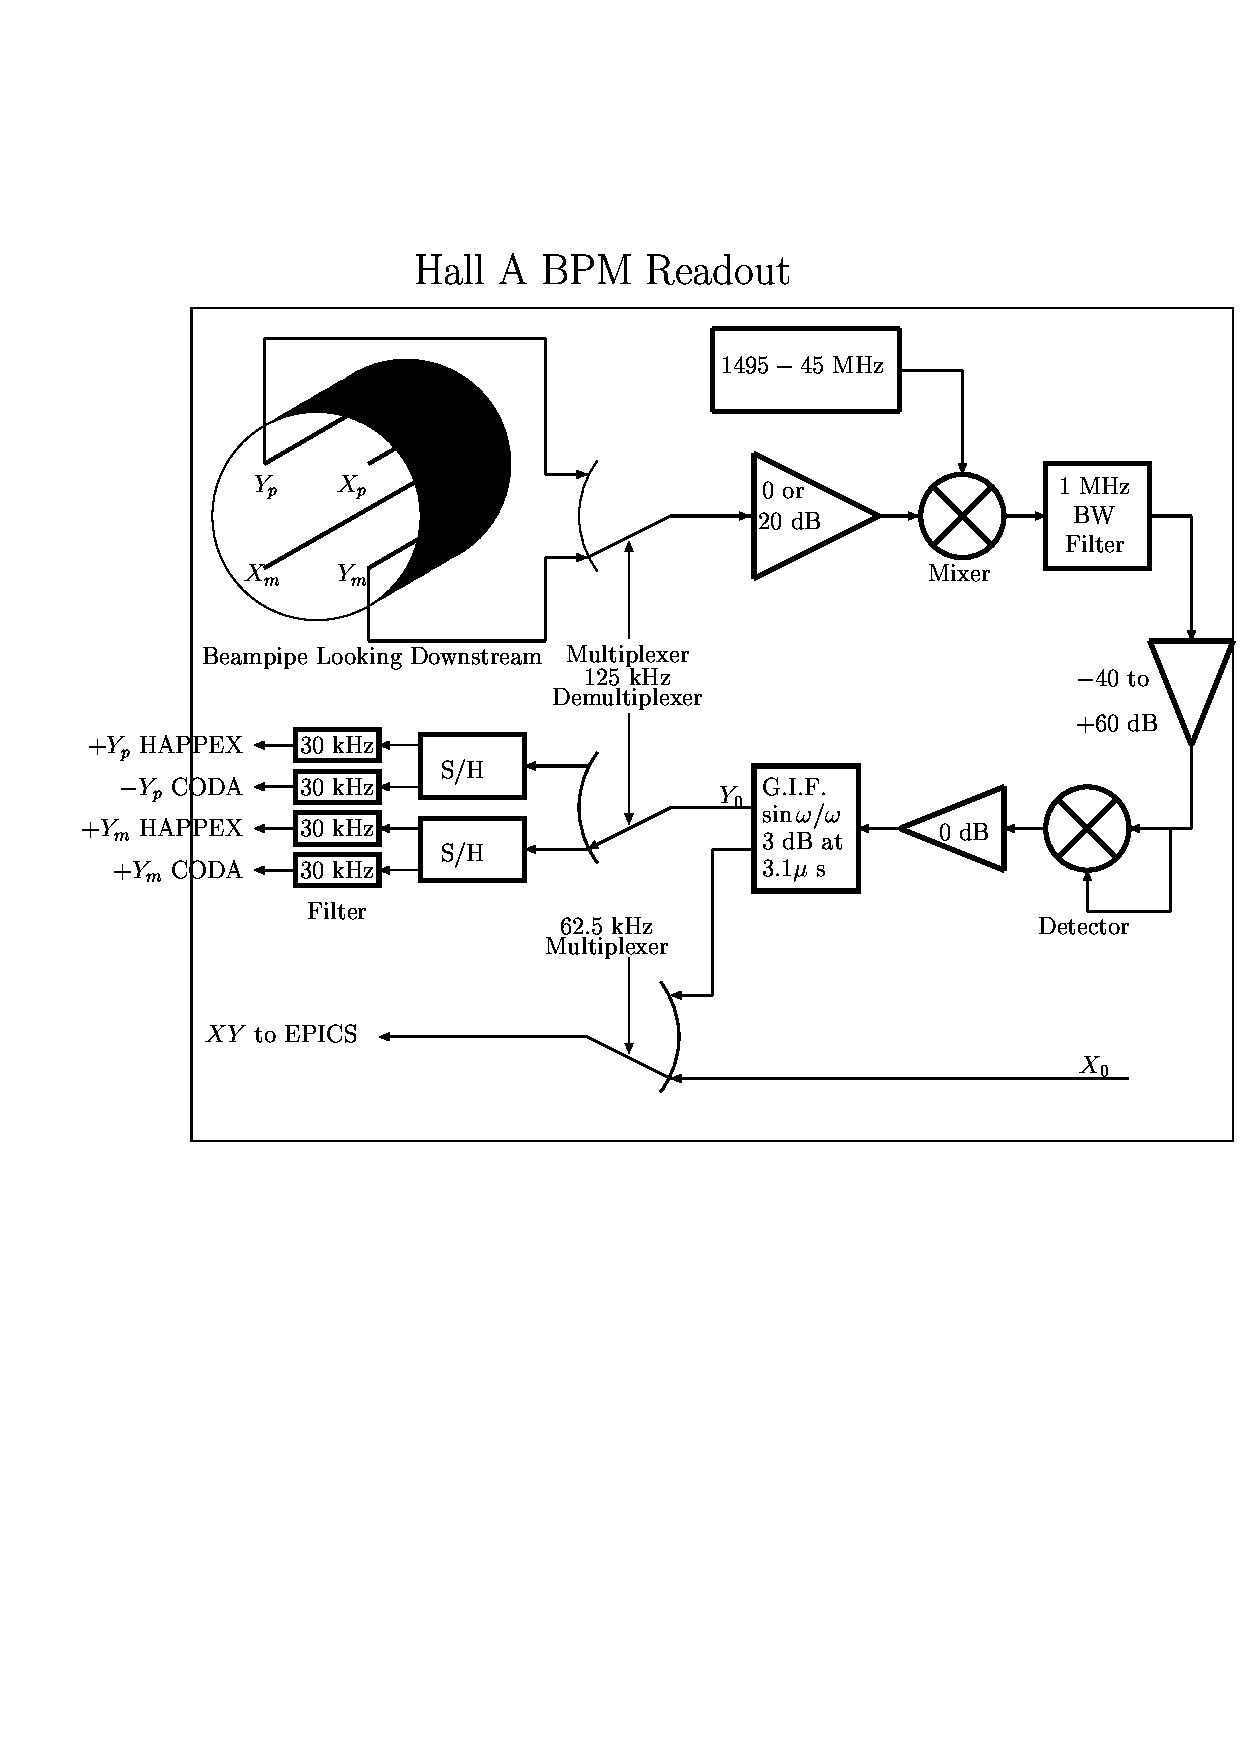
\includegraphics[angle=0,width=15cm]{BPM_fig}
{\linespread{1.}
\caption[Beamline: BPM Readout Electronics]{Schematic of the BPM readout
electronics}
\label{fig:bpmel}}
\end{center}
\end{figure}
}

1. The averaged position over 0.3 seconds is logged into the EPICS~\cite{EPICSwww} database (1 
Hz updating frequency) and injected into the datastream every 3-4 seconds, 
unsynchronized but with an orientative timestamp. From these values we can 
consider that we know the average position of the beam calculated in the EPICS 
coordinate system which is left handed.

2. Approximately once a shift (or more often if requested by the experimenters) 
a B-scope procedure ~\cite{bi:TP} can be performed using the same EPICS electronics 
which then gives the peak-to-peak variation of the beam.

3. Event-by-event information from the BPMs are recorded in the CODA datastream
from each of the 8 BPM antennas (2x4) from which the position of the beam can be 
reconstructed. However, these raw values belong to a parallel electronics chain 
whose constants have to be retrieved by calibrations to the EPICS or scanner 
data. 

\subsection{Beam Exit Channel}

After the target vacuum chamber, which was built by
the University of Virginia, there is an exit beam pipe which 
transfers the scattered beam onto the dump tunnel under vacuum. This exit beam 
pipe is made of a thin walled aluminum spiral corrugated pipe of welded 
construction. The largest diameter is 36 inches with a 0.164 inches wall 
thickness and the smallest diameter is 6 inches with a 0.042 inches wall 
thickness. The whole assembly is rather light (approximately 800 kg) and is 
supported by H shaped adjustable stands. To prevent possible linear collapse 
of the larger diameter sections under vacuum load, four aluminum channels of 
total cross-sectional area of 3'' are welded to its side. A vacuum of 
10$^{-5}$ Torr is maintained with a turbomolecular pump. The exit face of this 
pipe has a 12'' port and is connected to the diffuser with a Beryllium 
window.

}

\section{ Machine/Beamline protection system}
\label{sec:beam-fsd}

The MPS~\cite{MPScebaf} system is composed of the Fast Shutdown System (FSD), Beam Loss 
Monitor (BLM), and gun control system.

The FSD system is a network of permissive signals which terminate at the 
electron gun and chopper 1. The permissive to the gun and chopper
1 may be inhibited by any device connected to an FSD mode. Devices connected to the 
FSD system include vacuum valves, RF systems, Beam loss systems, beam current 
monitors, beam dumps, and particular to Hall A, the target motion mechanism 
and the raster (value and derivative).

The gun control system includes software program which monitors beam 
operating conditions and the state of the FSD and BLM systems. the program 
will warn the operators if a potential for beam damage exists. Potential for 
damage exists when running high average current beam, when FSD nodes are 
masked and when the beam power approaches the operating envelope limits for a 
specific beam dump.

\clearpage
\begin{safetyen}{10}{10}
\section{Safety Information}
\end{safetyen}
}
%
% Information for the ESAD
%

\begin{safetyen}{0}{0}

The beamline in the Hall provide the interface between the CEBAF accelerator
and the experimental hall.   All work on the beamline must be coordinated 
with both physics division and accelerator division; in order to ensure
safe and reliable transport of the electron beam to the dump.

\subsection{Hazards and Mitigations}

All magnets (dipoles, quadrupoles, sextupoles, beam correctors) and beam 
diagnostic devices (BPMs, scanners, Beam Loss Monitor, viewers) necessary for 
the transport of the beam are controlled by Machine Control Center (MCC) 
through EPICS~\cite{EPICSwww}, except for special elements which are addressed in the 
subsequent sections. The detailed safety operational procedures for the Hall 
A beamline should be essentially the same as the one for the CEBAF machine 
and beamline.\\ 

  
\noindent{}Personnel who need to work near or around the beamline should keep in mind the potential hazards:
\begin{itemize}
  \item Radiation ``Hot Spots'' - marked by ARM or RadCon personnel,
  \item Vacuum in the beam line tubes and other vessels,
  \item Thin windowed vacuum enclosers (e.g. the scattering chamber),
  \item Electric power hazards in vicinity of the magnets,
  \item Magnetic field hazards in vicinity of the magnets, and
  \item Conventional hazards (fall hazard, crane hazard etc.).
\end{itemize}

The most hazardous areas along the beamline are roped off it restrict access.   
In particule the scattering chamber, with it's large
volume and thin windows requires hearing protection once it has been evacuated.   
Signs are posted by radcon for any hot spots along the beamline and
radcon must be notified before work is done in a posted area.

Some magnets, as the M{\o}ller spectrometer elements, are covered with plastic
sheets for electric safety. Any access to these magnets requires
the ``Lock and Tag'' procedure~\cite{EHScebaf} and the appropriate training,
including the equipment-specific one. \\

\noindent{}Additional safety information is available in the following documents:
\begin{list}{--}{\setlength{\itemsep}{-0.15cm}}
  \item EH\&S Manual~\cite{EHScebaf};
  \item PSS Description Document~\cite{PSScebaf}
  \item Accelerator Operations Directive~\cite{AODcebaf};
\end{list}

\subsection{Responsible Personnel}

Since the beamline requires both accelerator and physics personnal to maintain
and operate and it is very important that both groups stay in contact that any 
work on the Hall A beamline is coordinated.

\begin{namestab}{tab:beam:personnel}{Beam line: authorized personnel}{%
   Beamline physics division and accelerator divison points-of-contact.}
  \namestabheader{Hall A Physicists}
  \DouglasHiginbotham{\em 1st Contact}
  \RobertMichaels{\em 2nd Contact}
  \namestabheader{Liaisons from Accelerator Division}
  \HariAreti{..to Physics}
  \YvesRoblin{..to Hall-A}
\end{namestab}
\end{safetyen}


\newpage
\section{ Beam Position Monitors}

To determine the position and the direction of the beam on the experimental 
target point, two Beam Position Monitors (BPMs) are located at distances 7.524 m 
(IPM1H03A) and 1.286 m (IPM1H03B) upstream of the target position. 
The BPMs consist of a 4-wire antenna array of open ended thin wire striplines 
tuned to the fundamental RF frequency of 1.497 GHz of the beam ~\cite{bi:bar90}. The 
standard difference-over-sum technique is then used ~\cite{bi:HW} to determine the 
relative position of the beam to within 100 microns for currents
above 1 $\mu $A. The absolute  position of the BPMs can be calibrated with respect to the 
scanners (superharps) which are located adjacent to each of the BPMs (IHA1H03A 
at 7.353 m and IHA1H03B at 1.122 m upstream of the target). The schematic of the 
readout electronics is shown in Figure ~\ref{fig:bpmel}. The
position information from the 
BPMs can be recorded in three different ways:

\begin{figure}
\begin{center}
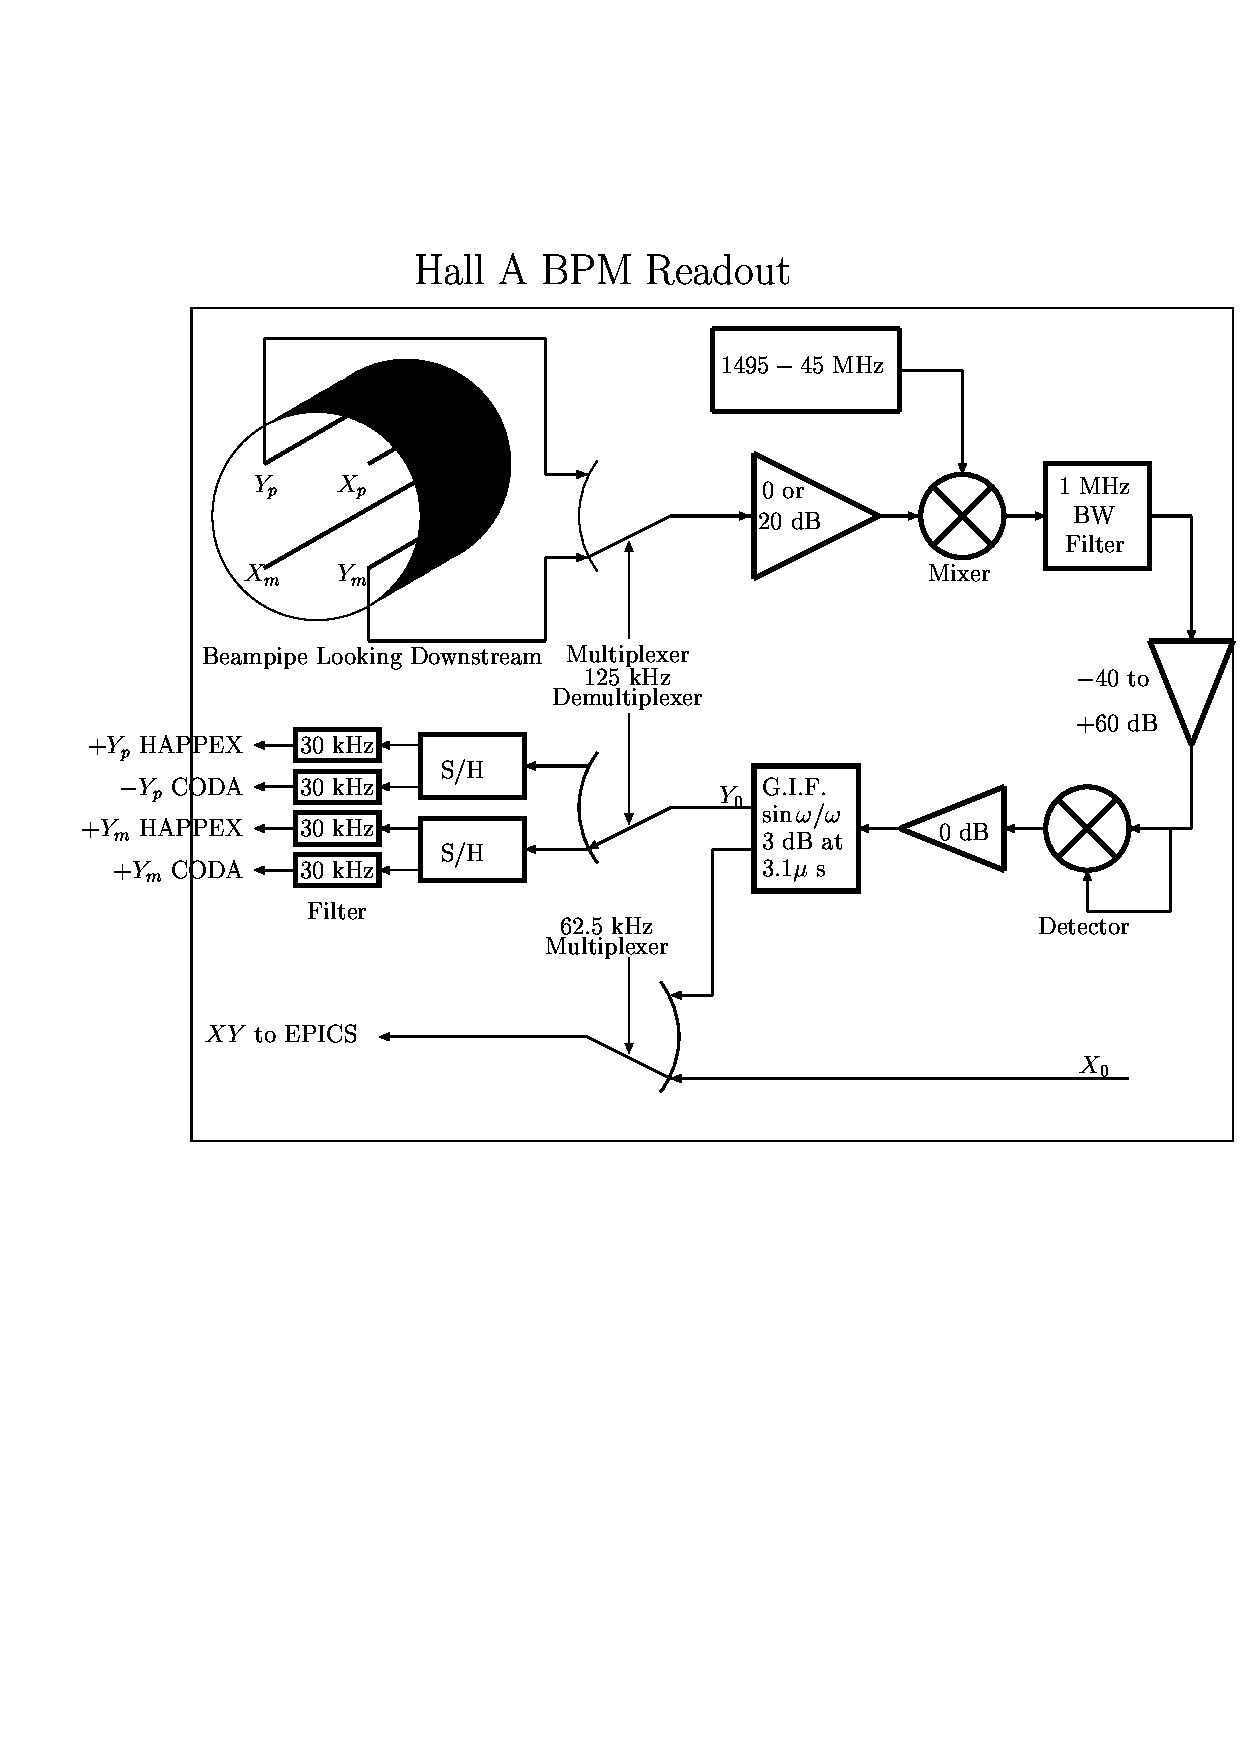
\includegraphics[angle=0,width=15cm]{BPM_fig}
{\linespread{1.}
\caption[Beamline: BPM Readout Electronics]{Schematic of the BPM readout
electronics}
\label{fig:bpmel}}
\end{center}
\end{figure}

\vskip 0.5cm

1. The averaged position over 0.3 seconds is logged into the EPICS database (1 
Hz updating frequency) and injected into the datastream every 3-4 seconds, 
unsynchronized but with an orientative timestamp. From these values we can 
consider that we know the average position of the beam calculated in the EPICS 
coordinate system which is left handed.

\vskip 0.5cm

2. Approximately once a shift (or more often if requested by the experimenters) 
a B-scope procedure ~\cite{bi:TP} can be performed using the same EPICS electronics 
which then gives the peak-to-peak variation of the beam.

\vskip 0.5cm

3. Event-by-event information from the BPMs are recorded in the CODA datastream
from each of the 8 BPM antennas (2x4) from which the position of the beam can be 
reconstructed. However, these raw values belong to a parallel electronics chain 
whose constants have to be retrieved by calibrations to the EPICS or scanner 
data. 


%\begin{thebibliography}{99}
%\bibitem{bi:bar90} W. Barry et al., CEBAF-PR-90-009 (1990).
%\bibitem{bi:HW} C. Hyde-Wright et al., Beam Position Studies for E93050 and priv. comm..
%\bibitem{bi:TP} T. Powers, priv.  comm.. 
%\end{thebibliography}
% ===========  CVS info
% $Header: /group/halla/analysis/cvs/tex/osp/src/beamline/bpms.tex,v 1.1 2003/06/05 17:28:32 gen Exp $
% $Id: bpms.tex,v 1.1 2003/06/05 17:28:32 gen Exp $
% $Author: gen $
% $Date: 2003/06/05 17:28:32 $
% $Name:  $
% $Locker:  $
% $Log: bpms.tex,v $
% Revision 1.1  2003/06/05 17:28:32  gen
% Initial revision
%

\newpage
\section[Beam Current Measurement]{Beam Current Measurement
\footnote{
  $CVS~revision~ $Id: bcm.tex,v 1.5 2003/12/13 06:23:37 gen Exp $ $
}
\footnote{Authors: A.Saha \email{saha@jlab.org}}
}

The Beam Current Monitor (BCM) is designed for stable, low noise, non-intercepting 
beam current measurements. It consists of an Unser monitor, two rf cavities, 
the electronics and a data acquisition system. The cavities and the Unser monitor 
are enclosed in a box to improve magnetic shielding and temperature stabilization.
The box is located 25 m upstream of the target. You can recognize it as a grey 
object on the stands, about 2 m downstream from where the beam enters the 
hall. 

The DC 200 down-converters and the Unser front end electronics are located in Hall 
A. The temperature controller, the Unser back end electronics and its calibration 
current source, cavity's RF unit (housing the RMS-to-DC converter board) and all 
multi-meters, VME crate and computers are located in Hall A control room.

\infolevone{
\subsection{ System Layout}

The schematic diagram of the BCM system is presented in
Fig.~\ref{fig:halla_bcm}.
\begin{figure}[htp]
\begin{center}
\includegraphics[angle=0,width=0.9\textwidth,clip]{habcm_r}
{\linespread{1.}
\caption[Beam Current Measurement: Schematic]{Schematic of the Hall A beam
current measurement system.}
\label{fig:halla_bcm}}
\end{center}
\end{figure}

The Unser monitor is a Parametric Current Transformer designed for non-destructive 
beam current measurement and providing an absolute reference. The monitor is 
calibrated by passing a known current through a wire inside the beam pipe and has a 
nominal output of 4 mV/$\mu $A. It requires extensive magnetic shielding and 
temperature stabilization to reduce noise and zero drift. As the Unser monitor's 
output signal drifts significantly on a time scale of several minutes, it cannot be 
used to continuously monitor the beam current. However, this drift is measured 
during the calibration runs (by taking a zero current reading) and removed in 
calibrating the cavities.  The more stable cavities are then used to determine the 
beam current and charge for each run. We also use the OLO2 Cavity Monitor and the 
Faraday Cup 2 at the Injector section to provide an absolute reference during 
calibration runs.

The two resonant rf cavity monitors on either side of the Unser Monitor are 
stainless steel cylindrical high Q ($\sim 3000$) waveguides which are tuned to the 
frequency of the beam (1.497 GHz) resulting in voltage levels at their   outputs 
which are proportional to the beam current. Each of the rf output signals from the 
two cavities are split into two parts. One part of the signal is  converted to 10 
kHz signals (by the ``downconverters'') and fed into an RMS-to-DC converter board 
consisting of a 50 kHz bandpass filter to  eliminate noise, amplified and split to 
two sets of outputs, which after further processing are recorded in the data 
stream. These two paths to the data stream (leading to the sampled and integrated
data ) will now be described. (The other part of the split signal is downconverted 
to 1 MHz signals and represents the old system (pre Jan 99). Only the HAPPEX 
collaboration presently uses these signals.)

For the sampled (or EPICS~\cite{EPICSwww} or Slow) data, one of the amplifier outputs is sent to a 
high precision digital AC voltmeter (HP 3458A). Each second this device provides 
a digital output which represents the  RMS average of the input signal during that 
second.  The resulting number is  proportional to the beam charge accumulated 
during the corresponding second (or, equivalently, the average  beam current  for 
that second). Signals from both cavity's multi-meters, as well as from the 
multi-meter connected to the Unser, are transported through GPIB ports to the HAC 
computer where they are recorded every 1 to 2 seconds via the data-logging process 
which is described in the calibration procedure. They are also sent through EPICS 
to CODA and the data stream where they are recorded at  quasi-regular intervals, 
typically every two to five  seconds.

For the integrated (or VTOF or Fast) data, the other amplifier output is sent to an 
RMS-to-DC converter which   produces  an analog DC  voltage  level. This level 
drives a Voltage-To-Frequency (VTOF) converter whose output frequency is  
proportional to the  input DC voltage level. These signals are then fed to Fastbus  
scalers and are finally injected into the data stream along  with the other scaler 
information.  These scalers simply accumulate during  the run, resulting  in a 
number which is proportional to the time integrated voltage level and therefore 
more accurately represents the true integral of the current and hence the total 
beam charge. The regular RMS to DC output is linear for currents
from about 5 $\mu$A to somewhere well above 200 $\mu$A.
 Since it is non-linear at the lower 
currents, we have introduced a set of amplifiers with differing gains (x3 and x10) 
allowing the non-linear region to be extended to lower currents at the expense of 
saturation at the very high currents. Hence there are 3 signals coming 
from each BCM (Upx1, Upx3, Upx10, Dnx1, Dnx3, Dnx10). All 6 signals are fed 
to scaler inputs of each spectrometer (E-arm and H-arm) . Hence we have a 
redundancy of 12 scaler outputs for determining the charge during a run. During 
calibration runs we calibrate each of these scaler outputs.   
}

\begin{safetyen}{10}{10}
\subsection{ Authorized Personnel}
\end{safetyen}

All Hall A members are authorized to take BCM calibration data using the Standard 
Non-Invasive Hall A BCM Calibration Procedure. The extended calibration procedures 
involving the Faraday Cup 2 and the OLO2 monitor at the Injector are presently 
performed by A. Saha. 

\vskip 0.2cm

The Accelerator AES group performs the maintenance of the BCM monitors. These 
include:

\begin{tabular}{l l}
1. The Unser calibration. & Every 3 months \\
2. Resonant Cavities Tuning. & Every Downtime \\
3. Multi-meters Autocalibration. & Every Downtime \\
4. Connectors Cleaning. &  Every year \\
5. Unser Keithley Current Source. & Calibration Yearly \\
6. Digital Multi-meters HP3458A and HP 34401A. & Calibration Yearly\\   
\end{tabular}

System Contacts are shown in Table~\ref{tab:BCM:personnel}.
\begin{namestab}{tab:BCM:personnel}{BCM: authorized personnel}{%
   Beam Current Monitor: authorized personnel}
  \ArunSaha{\em Contact}
  \JohnMusson{Accel. expert}
\end{namestab}
%Jean-Claude Denard -x 7555




% ===========  CVS info
% $Header: /group/halla/analysis/cvs/tex/osp/src/beamline/bcm.tex,v 1.5 2003/12/13 06:23:37 gen Exp $
% $Id: bcm.tex,v 1.5 2003/12/13 06:23:37 gen Exp $
% $Author: gen $
% $Date: 2003/12/13 06:23:37 $
% $Name:  $
% $Locker:  $
% $Log: bcm.tex,v $
% Revision 1.5  2003/12/13 06:23:37  gen
% Septum added. Name tables. Polishing
%
% Revision 1.4  2003/12/05 05:48:30  gen
% Polishing
%
% Revision 1.3  2003/06/06 15:19:02  gen
% Revision printout changed
%
% Revision 1.2  2003/06/05 23:29:59  gen
% Revision ID is printed in TeX
%
% Revision 1.1.1.1  2003/06/05 17:28:32  gen
% Imported from /home/gen/tex/OSP
%
%  Revision parameters to appear on the output

\newpage
\section[Fast Raster]{Fast Raster
\footnote{Authors: R.~Michaels \email{rom@jlab.org}}
}


The beam is rastered on target with an amplitude of
several millimeters at 25 kHz to prevent overheating.  
The raster is a set of four of air-core dipoles located
approximately 23 m upstream of the target. 
Two dipoles are for horizontal (X) motion and
another two for vertical (Y).  During the 6 GeV era
there was only one pair of X and Y, but we have doubled
the raster to account for the energy increase to 11 GeV.
The arrangement along the beamline along the 
direction of the beam will be XXYY.

For a typical 40A current in the raster coils, the
deflection by one pair (e.g. the X direction) of coils, 
in radians, is $\theta = 1.94 \times 10^{-3}/ E$
where $E$ is the electron's energy in GeV.
For example, at $E = 6$ GeV, a 0.32 mrad deflection is achieved.
Projected onto the target (about 21 m away) this is a $\pm$ 6.8 mm
excursion {\it if} there were no other magnetic fields 
between the raster and the target; however, there are quadrupoles
which change this depending on the beam tune.

Since 2003 we've used the triangle-wave 
raster pattern designed by Chen Yan.  
This achieves a very uniform rectangular
density distribution of beam on the target 
by moving the beam with a time-varying dipole
magnetic field whose waveform is triangular
with very little dwell time at the peaks.  
The electronics design is an ``H-bridge''
in which switches are opened and closed 
at 25 kHz, to switch between two directions 
of current (100 A peak-to-peak) 
through the raster coils.

Three new features during the 12-GeV era are 
1) the driver of the H-bridge electronics is now
an Agilent model 33522A waveform generator; and
2) The two X are synchronized with each other, and
the two Y are synchronized.  This makes the kicks
add and allows us to accomodate the higher energy
of the beam; and 3) The entire raster can
be synchronized to an external 10 MHz wavetrain
supplied by the polarized injector electronics.
This makes the nominal 25 kHz an exact multiple of
the helicity-flip rate, which achieves a cancellation
of raster noise, important for parity-violation 
experiments only.
The syncrhronization of the pairs of X and Y are
accurate to within a few nsec.

For most users, these three new features will not be
noticeable and the raster will appear to function
the same as during the 6 GeV running.
A user can view the 
status of the raster in the
EPICS overview screen called ``General Accelerator
Parameters'' where the set-point for the radius amplitude
and the readback of the peak-current in the raster are displayed.

Control of the raster is done by first asking the MCC
operators to set up the raster for a particular size
typically 2 mm square.
The control software assumes a field-free region between
the raster and the target, so it is only approximately
correct because there are several quadrupoles in this region.
It is important to check the raster spot size and
make adjustments if necessary.  The adjustment is made
by asking MCC to change the size and noting the 
linear relationship between what their software says
the size is and the actual size.
Relatively small independent adjustments to the 
gains on the X and the Y raster
coils are available in the middle room of the hall A
counting room using the ``PGA Controller'' knobs;
however, it is not recommended to touch these.
Near these knobs is also located an oscilloscope X-Y trace
of the current in the raster.  A fast shutdown (FSD) shuts
the beam down within 0.1 msec if the raster fails, thus
affording some protection of the target.

{\it NOTE:  If you are unsure of the status of the raster,
measure the spot size with very low current ($\le 2 \mu$A) or with
the target out of the beam.}  It would be a mistake
to check the beam spot size with high current on target; by
the time you check it, the target may already be destroyed.
The rastered beam spot on target can be checked with
plots in the ROOT analyzer or by 
using the stand alone code called \mycomp{spot},
also called \mycomp{raster}.
For more details on usage, type \mycomp{spot -h} (help)
on the ADAQ computers.

Regarding the BPM measurements, it should be noted that 
the stripline BPMs displayed by \mycomp{spot} have a high-frequency 
cutoff of approximately 30 kHz.  Since the raster frequency is 25 kHz
the plot of the amplitude distribution shows spikes at the 
limits of the orbit, instead of a flat distribution.  The scale
factor between what is seen in \mycomp{spot} and the real width of the beam
is $\sim 1.5$, i.e. the beam is 1.5 times bigger than the naive
reading of the \mycomp{spot} distribution.



\newpage
% Updated Comments Dec. 2
\infolevone{
\chapter[Arc Energy Measurement]{Arc Energy Measurement
\footnote{Authors: D. Higinbotham \email{doug@jlab.org}}
}
}

\infoleveqnull{
\section{Arc Energy Measurement}
\subsection{Overview}
In order to determine the integral field of the eight dipoles that lead to Hall A, and 
in turn determine the beam energy, a nineth dipole wired in series with the rest is 
located in a special shed near the hall A counting house.
}

\infolevone{
The ARC energy measurement is under EPICS~\cite{EPICSwww} control through 
a MEDM~\cite{MEDMwww} display. Two
independent control systems are used: the beam bend angle measurement through
the arc ("scanners") and the field integral of
the arc ("integral"). To measure the energy: 

\begin{itemize}
\item perform several angle measurements 
\item perform an integral measurement 
\item analyze the integral measurement and note the value of the arc field 
integral 
\item analyze the angle measurements, average the results (proposed by the 
software),
then ask for the energy calculation, enter the above arc field integral and
you will get the beam energy computed from the average angle. 
\end{itemize}

\section{Summary of ARC operations }

Six scanners of the same type, called ``ARC scanner'' and labelled
from scanner \#1 to \#6, are installed on the Hall-A beamline. Scanners \#1
to \#4 are used for the ARC energy measurement and they are located on the Hall-A
arc: \#1 [1HA1C07A] and \#2 [1HA1C07B] just upstream of the arc, in the BSY, and 
\#3 
[1HA1C18A] and \#4 [1HA1C18B] in the Hall-A
tunnel, just upstream the Compton polarimeter. Scanners \#5 [1HA1H03A] and \#6 
[1HA1H03B] 
are located
between the Moller and the target to control the beam geometry on the target
and their use will not be discussed here. 

Procedure for running a harp scan is described elsewhere\footnote{
Harp scan procedure \url{http://hallaweb.jlab.org/equipment/beam/harp_halla/harp.html}.}

Each scanner has a motor/ball-screw/shaft-encoder/vacuum-penetrator system moving
accurately a set of 3 tungsten wires through the beam. Each time a wire crosses
the beam a PMT located a few meters downstream records a signal due to the 
electromagnetic
shower induced by the beam in the wire. Both forward and backward passes are
recorded. The motion is a horizontal translation and, for a forward pass: 

-the translation is from beam left to beam right, 

-the two first wire crossing the beam are at 45deg from the vertical, 

-the third wire, which is the only important for the ARC energy measurement,
is vertical. 

Recording, during the scan, the scanner position and the PMT output voltage
allows us to determine the beam position at each scanner location. Then, using
calibration data not detailed here, we deduce the net beam bend angle through
the arc. This result measured in dispersive arc tuning, along with the field
integral of the arc dipoles, provides an accurate determination of the beam
energy. 

\vspace{0.3cm}

\section{Summary of field integral }

The purpose is to measure absolutely the straight field integral of a 
"BA"
3m long dipole, called the "9th dipole" and located in the
"Dipole Shed". It is of the same type as the 8 arc dipoles
and is powered in series with them. 

The ARC integral setup is basically made of a 3m long plate (the 
"probe")
which is able to move inside the 9th dipole gap along the beam axis and carrying 
two
field measurement devices: a pair of pick-up coils connected in series and a
set of NMR probes. The coils are on both ends of the probe and the NMRs close
to the center. 

-at the "upstream" probe position, the 
"downstream"
coil is close to the dipole center, the "upstream" is outside
the dipole and the NMRs at one end of the dipole: 

Door$<-$-- ....................$<-$-------DIPOLE-----$--->$ 

.............$<-$-------PROBE------$--->$ 

-at the "central" probe position, each coil is at one end
of the 3m long dipole and the NMRs close to the dipole center: 

Door$<-$-- ...................$<-$-------DIPOLE-----$--->$ 

..................................$<-$-------PROBE------$--->$ 

-at the "downstream" probe position, the 
"upstream"
coil is close to the dipole center, the "downstream" is outside
the dipole and the NMRs at one end of the dipole: 

Door$<-$-- ...................$<-$-------DIPOLE-----$--->$ 

....................................................$<-$-------PROBE------$--->$ 

We call upstream the position where the probe is the closest to the shed access
door. Among the 3 above positions, the only one where the NMR can lock on the 
dipole
field is the central one as in the extreme position of the probe, the field 
homogeneity
is not sufficient. The probe position is controlled by a linear encoder. The
Z axis refers to the "beam" direction, increasing from upstream
to downstream. We use three kinds of "Z": 

-Zm to locate a point inside the magnet. The dipole center is at Zm=0 and the
yoke ends at +-1500.mm 

-Zp to locate a point inside the probe. The probe center is at Zp=0. Each of
the 4 NMR probes has a Zp given in the file "magnet.dir".
At a temperature of 21C, the coils are at Zp=+-1519.815mm (from magnet.dir) 

-Zd to refer to a displacement of the probe w.r.t. the dipole. Zd=0 refers to
the upstream (home) position of the probe. The integral measurement is performed
from Zd=0.000mm (1st PDI trigger) to Zd=3199.000mm (last PDI trigger), for forward
pass. Zd is given by the display (at the top of the rack) or by the master screen
("OUT"). 

The relationship between Zm, Zp and Zd is: 

Zd-Zm+Zp=C 

where C is a constant given in magnet.dir (C=1604.000 nomin.). Example of use:
to have the probe center at the dipole center, one must set Zd=1604.000mm (set
Zm=0 and Zp=0 in the above formula, and solve for Zd) 

The integral measurement sequence is the following: 

-from the current position (a priori arbitrary) move the probe upstream, up
to a limit (optic) switch. 

-move downstream by a few mm to cross the encoder index (encoder initialization) 

-move to the central position to measure the central field by NMR, the system
checks if the NMR locks and if the reading is stable, it will be the 
"before"
field 

-move back to upstream position 

-move to downstream position while integrating the flux through the coil system,
this measurement will be called the "forward" integral (duration
\( \sim  \) 7s) 

-move back to upstream position while integrating the flux through the coil
system, this measurement will be called the "backward" integral
(duration \( \sim  \)7s) 

-move to the central position to measure the central field by NMR, the system
checks if the NMR locks and if the reading is stable, it will be the 
"after"
field. 

In addition to the central field, 4 probe temperatures, a local excitation current
measurement, the setting of the dipoles P.S, the readback of the dipoles P.S
and the probe position at NMR measurement time are recorded 
"before"
and "after". 

To perform an integral field measurement: 

1-check if the system works (see "details on integral system 
check"
below) 

2-run the above integral sequence (see "details on integral run"
below) 

3-fix the error(s) if any (see "details on integral errors"
below) 

4-save the data in a file (see "details on integral data save"
below) 

5-analyze the data  


\section{Details on integral run }

To run the integral measurement sequence, call the 
\mycomp{arc\_integral.adl}
medm screen, then: 

-push "start" to start the full sequence 

-look at the results displayed: 

-after the "before" NMR measurement: the 
"before"
data set 

-after the "forward" integral pass: the forward velocity profile
and the forward voltage-after-gain profile 

-after the "backward" integral pass: the backward velocity
profile and the backward voltage-after-gain profile 

-after the "after" NMR measurement: the 
"after"
data set 

-if "BAD NMR" or "PDI saturation" flags
are set, or if something is obviously wrong in the data or plots, call expert. 

-data are ready to be saved (see "Details on integral data save"
below) 


\section{Details on temperatures }

The AC system of the shed is made of two cooling units, a heating unit and a
controller connected to two temperature sensors : one located in the shed and
one located in the BSY. This system is programmed in such a way that the 
temperature
of the shed follows the BSY temperature within +-2C. The BSY temperature can
be anywhere in the 18C to 35C range, regardless of the season. The BSY 
temperature
and the shed temperature are given (in F) by a display panel located close to
the workstation, on the wall. The AC system can be set in manual control by
turning from "auto" to "manual" a set of
switches controlling the cooling units and the heater unit. These switch boxes
are located on the shed wall. If the shed temperature is above 34.4C (94F),
call the crew chief (the electronics can be damaged) and cool down the shed in manual
AC mode. The 4 temperature sensors of the probe are labelled Tx+z+, Tx+z-, Tx-z+,
Tx-z- depending on their position w.r.t. the frame. 

Both "x+" sensors are on the probe edge which is inside the
dipole gap and both "x-" sensors on the opposite edge which
is outside the dipole gap. Both "z-" sensors are at 1/4 of
the long dimension of the probe and both z+ at 3/4 of this length. The average
of the 4 temperatures is used by the analysis program to correct the coil distance
from the thermal expansion of the probe, so it is important to make sure that
the 4 sensors are working well. The user can just make sure that the temperatures
displayed in \mycomp{arc-master.adl} or recorded in 
\mycomp{arc-integral.adl}
are realistic. In \mycomp{arc-integral.adl} they are given in the
order: Tx+z-, Tx+z+, Tx-z-, Tx-z+ Tx-z- and Tx-z+ should be close to the shed
temperature. Tx+z- and Tx+z+ depend on the probe position, as the gap (iron
yoke) is warmer than the shed and the dipole coil (at both ends of the dipole)
is warmer than the iron yoke. For a probe in a central position for more than
about one hour, the Tx+z- and Tx+z+ sensors should give the yoke temperature,
i.e the shed temperature plus 0. to 5.C, depending on the current, LCW temperature
and the magnet/shed temperature history. The 4 temperatures are also displayed
inside the shed, on the electronics rack. These values are digitized by separate
ADCs, so they may differ from the remote values by \( \sim  \)0.1C. 
}

\begin{safetyen}{10}{10}
\infolevone{\section{Shed access and safety }}

Due to the the dipole magnet and motion system, the access to the shed is limited to authorized
persons which are listed in the ESAD and listed below. To be added to the list, 
contact Douglas Higinbotham.
The standard
operation mode of the integral measurement setup is the remote mode, through
the network, from the counting house.
\end{safetyen}

\begin{safetyen}{10}{10}
\infolevone{\section{List of Authorized Personnel for Shed Access}}
\infoleveqnull{\subsection{List of Authorized Personnel for Shed Access}}
\end{safetyen}
\begin{namestab}{tab:arc:personnel}{Arc Energy Measurement: authorized personnel}{%
                 Arc Energy Measurement: authorized personnel}
  \namestabheader{Hall A Personnel}
  \DouglasHiginbotham{\em Contact}
  \namestabheader{Accelerator Personnel}
  \MichaelTiefenback{}
  \YvesRoblin{}
  \RickGonzales{}
  \BillMerz{}
  \MarkAugustine{}
  \HariAreti{}
  \PeteFrancis{}
  \ScottHiggins{}
  \DavidSeidman{}
  \RonLauze{}
  \TonyDay{}
  \ChristopherCurtis{Alignment group}
  \namestabheader{CEA - Saclay experts}
  \PascalVernin{}
  \ChristianVeyssiere{}
  \FrancoisGougnaud{}
  \JacquesMarroncle{}
\end{namestab}



\newpage
\infolevone{
\chapter[Target Chamber]{Target Chamber
\label{sec:target_chamb}
\footnote{
  $CVS~revision~ $Id: tgtcham.tex,v 1.11 2005/04/04 22:27:25 gen Exp $ $
}
\footnote{Authors: ?? \email{??@jlab.org}}
}

The cryo-targets and the waterfall targets 
(see Sec.~\ref{sec:targets-overv}) 
are contained in a special target chamber which is a large 
evacuated  multistaged can. So far, three chambers have been designed:
\begin{list}{\arabic{enumi}.~}{\usecounter{enumi}\setlength{\itemsep}{-0.15cm}}
  \item a chamber used up to 2003;
  \item a chamber designed for use with septum magnets, starting in 2003;
  \item a chamber designed for use with the BigBite spectrometer.
%\footnote{
%        No yet manufactured by Dec,2003.}.
\end{list}

Here, chamber 1 is described. Chambers 2 and 3 are only different in 
size and slightly in shape. The safety considerations fully apply to chambers 2 and 3.
The chamber was designed to isolate the beam line vacuum from  each
HRS so that each HRS could rotate
around the target without vacuum coupling and without jeopardizing
certain desired kinematic and acceptance  specifications of 
both high resolution spectrometers
needed for approved experiments.  It  was also designed to simultaneously
 contain a liquid or gas target and an array of water cooled thin
 metallic foils, both remotely controlled and also be adaptable for
the waterfall target. The desired kinematic specifications that were
 considered included momentum and energy resolution in both arms,
 angular range of spectrometers, angular acceptance, and luminosity.
The chamber vacuum is isolated from the  HRS by using thin aluminum foils. 

The target chamber is designed so that
each spectrometer will have continuous coverage in the standard tune from
$\theta_{min}=$12.54$^\circ$ to $\theta_{max}=$165$^\circ$.
The aluminum window is 6~$in$ high and 0.016~$in$ thick made of 5052 H34 aluminum foil.
The foil forms regularly spaced vertical ridges when
placed under load. The window had an inter-ridge
spacing of 3 inches.
If the window is treated as a collection
of smaller rectangular windows which have the full vertical height
of 6 inches and the inter-ridge spacing as a width,
then stress formulas predict that the 0.016 $in$
material would reach ultimate stress at a pressure higher than 35 PSID
(for both over-pressure and under-pressure). 
There is a gate valve between the 
scattering chamber and the beam entrance (exit) 
pipe. Both 
valves will be closed automatically in the
event that the chamber vacuum begins to rise and an FSD will be caused
( this is done via a relay output of the scattering
chamber vacuum gauge). If either valve is closed an FSD will result.

The target chamber is supported by a 24 $in$ diameter pivot post
secured in concrete, rising about 93.6 $in$ above the Hall A cement floor.
The Hall A target chamber
consists of an aluminum middle ring, a stainless steel base ring,
each with a 41.0 $in$ inner diameter,
and a stainless steel cylindrical top hat with 40 $in$ inner diameter
to enclose the cryotarget and secure the cryogenic connections.

When the scattering chamber is under vacuum, there is a potential
danger of window rupture.
The loud noise from the rupture could hurt
one's ears if not protected. Therefore when the chamber is under vacuum,
protective covers are put on if possible. These must be taken off
for data taking. For restricted access, the protective cover is required
to be on when the chamber is under vacuum. Before switching from controlled
access to restricted access, the protective cover is required to be installed.
Anytime that the scattering chamber
is under vacuum, the pivot area is enclosed in a rope or tape barrier
and a warning sign is posted.
Hearing protection is required in the enclosed area.

\infolevone{
	The aluminum ring with an outer diameter of 45.0 $in$ and
wall thickness 2.0 $in$  is necessary for a sturdy support structure and
to permit machining of the outside surface to accommodate
the flanges for fixed and sliding seals mounted on
opposite sides of the ring that vacuum connect the chamber to each HRS.
The height of the aluminum ring shown is 36.0 $in$, which is
designed to accommodate the mounting flanges.
The stainless steel base ring 
is 11.50 $in$ in height with
one pump-out 6 $in$ diameter port  and with
seven 4 $in$ viewing and electrical feed-through ports.
The base ring will also contain support mechanisms for the solid
target ladder assembly, a rotisserie for collimating slits, radiators, and
magnetic
fingers for
removing the solid target vacuum-lock can. The total height of the top
ring, middle ring, and
base ring is 93.81 $in$. This length is partly determined by our desire to
include with the cryogenic extended target a solid target vertical ladder
secured in an inverted hat through a hole in the base of the chamber.

	The base ring includes an end plate through which the
inverted hat will be adapted to fit into the large vertical pipe serving
as the pivot post for the Hall A spectrometers.

	The stainless steel cylindrical top hat  has
40.0 $in$ inner diameter, and is 0.375 $in$ thick and
46.31 $in$ high , which is necessary to permit the
cryotarget to be withdrawn and to make space available to expose the solid
targets to the electron beam.

   The 200 $\mu$A electron beam, focused to a $\sim$\(0.1\, mm\times
0.1\) mm spot and rastered $\pm$5 mm horizontally or vertically on the
target, enters through a oval hole in the middle ring which
is 2.06 $in$ wide and exits through a 1.81 $in$ hole connected to the
exit pipe.
}

\infolevone{
\section{Target Chamber - Spectrometer Coupling}

   The aluminum middle ring will support a flange on each side for each high
resolution spectrometer. Four flanges will be available: Two flanges will
contain a 6 $in$ window opening which will be covered with a thin foil
(e.g., 10 mil aluminum) .
These two flanges will be used for experiments utilizing
extended  targets that do not require optimum momentum resolution.
The other two flanges will have two fixed ports (with a 8 $in$ $\times$ 6 $in$
opening)
which will be mainly used for calibration of the spectrometers . Fixed ports are
centered at 16.11 $^\circ$ and
45 $^\circ$ for one flange and at 16.11 $^\circ$ and 90 $^\circ$ for the second
flange.

   For a point beam on target a vertical opening in the walls of the chamber
of height 57.15 cm x 0.065 x 2 = 7.43 cm is required so that the scattered
beam is within the full acceptance of the spectrometer.
If the beam is rastered on target $\pm$0.5 cm in the vertical direction,
then the opening in the outer side of the chamber must be at least 8.5 cm for
full acceptance.

From consideration of the angular range of the spectrometers in the standard
tune, the scattered beam acceptance envelope, the effects of an
extended gas target on acceptance,
and the effects of a rastered beam $\pm$ 5 mm on acceptance,
the target chamber requires a window of at least 8.5 cm
high in the aluminum ring extending from 6.33 $^\circ$ (2.48 in) from the
beam exit point to 8.83 $^\circ$ (3.47 in) from the beam entrance point on one
side and a similar window on the other side of the beam.
For future considerations (e.g., using a third arm or sliding seal) the
width of the window on the middle ring was actually constructed
to be 17.78 cm (7 $in$).

\section{Stress Analysis of the Middle Ring}

Since the middle ring has an extensive cut across the midplane on both sides as
well as
entrance and exit holes and loaded with about 25,000 lbs, calculations of the
stresses
 and deformation of  the
midplane support area of the middle ring and deflection of the window opening
were made using the finite element analysis code ANSYS . The work was conducted
by a graduate student in the Department of Civil Engineering at the
University of
Virginia and a REU student.  A scaled down model of the middle ring was
constructed and then tested by applying forces to it using the Materials Testing
Service of the Department of Transportation at the University. ANSYS was first
checked by comparing calculations of the test model deflections to the actual
data. Agreement was  within $\pm$10\%. Results of ANSYS for the target
chamber showed that the maximum deflection of the opening of the window in the
middle ring varied from 0.007 $in$ to 0.015 $in$ depending on how the
middle ring
was loaded. This was decided to be a safe limit. In the final design, several
movable
7 $in$ long, 2 $in$ diameter aluminum support rods are placed in the
window for added support. In addition, flanges defining the ports and
coupling to
the spectrometers can be added, giving additional support to the middle ring.
Compressional stresses, calculated using ANSYS assuming the middle ring was
attached to the
top hat and loaded with 25,000 lbs, were less than 3000 psi 
almost everywhere.
However, stresses over small areas rose to levels 6000 psi near the entrance
and exit holes. These calculations indicated that we did not exceed the safety
limit of 15,000 psi for aluminum. A simple model calculation shown in Appendix
A  gives the result 1434 psi, which represents some average value over the
midplane
contact area.

\section{Vacuum Pumping System}

The vacuum in the target chamber is maintained by an Alcatel ( 880 l/s)
 turbomolecular vacuum pump. The pump is connected to a 6 $in$ port in the
stainless steel ring between 130
 $^\circ \le \theta_p \le 180 ^\circ$. The vacuum pump is
fastened to a horizontal pipe connected to the chamber. The vacuum pressure in
the chamber is about $10^{-5}$ mm. An additional Alcatel pump connected
to an 8 $in$ port should be added to obtain lower vacuum. Both
pumps may be isolated
from the target chamber using gate valves which are remotely operated
from the vacuum control rack and interlocked to the FSD system.


A 2 $in$ all metal gate valve is located between the entrance flange to the
chamber and the beam profile monitor.   
 An additional gate valve is located 2 m downstream of the
 target chamber to isolate the chamber from the exit beam pipe.
}
\begin{safetyen}{10}{15}
\section{Safety Assessment}
\end{safetyen}

The scattering chamber is typically a low maintenance item but it is a vacuum
system and hence problems may occur. The day to day operations of the cryogenic
targets are managed by the Hall A Staff while major maintenance operations are
handled by the Cryogenic Target Group (Physics Division). Occasionally the
cryogenic targets experience difficulties due to failures of the End Station
Refrigerator which supplies the coolant. In these cases the Cryogenics Group
of the Accelerator Division should be contacted.

\noindent{}The target chamber may pose several hazards:

\begin{list}{\arabic{enumi}.~}{\usecounter{enumi}\setlength{\itemsep}{-0.15cm}}
  \item {\bf Rupture of vacuum windows}. This hazard is mitigated by
        lexan guards on the vacuum windows, installed by the hall technicians
        either at the beginning of a ``restricted access'' period 
        %(see Sec.\ref{sec:Access}),
        or during ``control access'', in case an access to the target chamber area is needed.
        Installation and removal of the guards is included in the technician's checklists.
        When the chamber is under vacuum, it is mandatory to use ear protection in the chamber
        vicinity. The appropriate signs must be installed by the technicians. 

  \item {\bf Induced radioactivity}. The RADCON surveyor measures the level of induced
        radiation as a part of the general survey and may declare the target area 
        as ``High Radiation Area'', installing a rope protection around\cite{RWIcebaf}. 

\end{list}

Some other safety issues are discussed in the cryo-target chapter 
(see Sec.~\ref{sec:target-cryo-safety}).
%and also in the polarized target chapter (see Sec.~\ref{sec:target-he3-general}).

\begin{safetyen}{10}{15}
\section[Authorized  Personnel]{Authorized  Personnel}
\end{safetyen}

\begin{namestab}{tab:targ_chamb:personnel}{Target chamber: authorized personnel}{%
      Target chamber: authorized personnel. ``W.B.'' stands for the white board 
      in the counting house.}
  \TechonCall{\em Contact}
  \JessieButler{}
  \DaveMeekins{Target group}
  \JianPingChen{}
\end{namestab}
}

\newpage
\infolevone{\chapter[M{\o}ller Polarimeter]{M{\o}ller Polarimeter}
\setcounter{subsection}{0}}
\infoleveqnull{\section[M{\o}ller Polarimeter]{M{\o}ller Polarimeter}}

The Hall A beam line is equipped with a M{\o}ller 
polarimeter
whose purpose is 
to measure the polarization of the electron beam delivered to the hall. 

\begin{safetyen}{0}{0}

The M{\o}ller Polarimeter system has under gone a major upgrade and an Operational Safety Proceedure (OSP)
is being written and must be reviewed before its use.

\subsection{Hazards and Mitigations}

The hazards and mitigations for this system can be found in the OSP at the end of this document. 

%\infolevone{
%Safety checklist item for this device, located at the end of the beamline section, is solely to ensure
%the beam can be tranported safetly past this system prior to it's recommisioning.
%}

\subsection{Responsible Personnel}
\label{sec:moller-pers}

This list of system experts provided in case there is any question as to the status of system.

\begin{table}[h]
\begin{center}
\begin{tabular}{|ll|l|l|l|l|r|} \hline
  \multicolumn{2}{|c|}{Name} & Dept. & \multicolumn{2}{c|}{Telephone} & 
  \multicolumn{1}{c|}{e-mail} & Comment \\ 
  \cline{4-5}
   &  &   & JLab & Pager &  & \\ 
\hline
 Javier       & Gomez           & JLab    & 7498 & 7498 & gomez@jlab.org    & Primary contact     \\ 
 Oleksandr    & Glamazdin       & Kharkov & 5441 & 5441 & glamazdi@jlab.org &  \\ 
 Viktor       & Gorbenko        & Kharkov & 5441 &   -  & gorbenko@jlab.org &  \\ 
 Roman        & Pomatsalyuk     & Kharkov & 5395 & 0001 & romanip@jlab.org  &  \\ 
\hline
\end{tabular}
\end{center}
\caption[Moller Polarimeter: authorized personnel]{
   The listed name are those who are considered system experts of the Moller Polarimeter and should be contacted
   if there is any question as to the status of the system.
}
\label{tab:moller:personnel}
\end{table}
\end{safetyen}


\newpage
}
% Compton Polarimeter
\infolevone{\chapter[Compton Polarimeter]{Compton Polarimeter}
\label{sec:compton}
\footnote{Author: S.Nanda \email{nanda@jlab.org}}
}
\infoleveqnull{\section{Compton Polarimeter}
\subsection{Overview}}


The Hall A Compton polarimeter has undergone a major upgrade and an
new operational safety proceedure (OSP) is being written and reviewed before the
Compton can be used.   The hazards and mitigations for this system can be found in 
this OSP.

\subsection{Responsible Personnel}

\begin{namestab}{tab:compton:personnel}{Compton Polarimeter: authorized personnel}{%
          Compton Polarimeter: authorized personnel}
 \SirishNanda{Primary Contact}
 \JackSegal{Secondary Contact}
\end{namestab}

\infolevone{
\subsection{Authorized Personnel}

The list
of the presently authorized personnel is given in Table~\ref{tab:compton:personnel}.
Other individuals must notify and receive permission from
the contact person (see Table~\ref{tab:compton:personnel}) to get their names
add to list.

\begin{namestab}{tab:compton:personnel}{Compton Polarimeter: authorized personnel}{%
          Compton Polarimeter: authorized personnel}
 \SirishNanda{\it Contact}
 \JackSegal{Technical}
 \JosephZhang{Optics}
 \MartialAuthier{Engineering}
 \NathalieColombel{Mechanical}
 \PascaleDeck{Electronics}
 \AlainDelbart{Optics}
 \DavidLhuillier{Analysis}
 \YvesLussignol{EPICS}
 \DamienNeyret{DAQ}
 \GerardTarte{Electronics}
 \ChristianVeyssiere{Electronics}
\end{namestab}
}



%
% Old Material
%
% \chapter[eP Beam Energy Measurement]{eP Beam Energy Measurement
\footnote{
  $CVS~revision~ $Id: ep.tex,v 1.6 2003/12/13 06:23:37 gen Exp $ $
}
\footnote{Authors: B.Reitz \email{reitz@jlab.org}}
}
\label{sec:ep}
\section {Purpose and Layout}
\label{sec:ep_purpose}

The Hall A eP system is a stand-alone device to measure the 
energy of the electron beam. It is located along the beamline
17~m upstream of the target. The beam energy $E$ is determined by measuring
the scattered electron angle $\Theta_e$ and the recoil proton angle
$\Theta_p$ in the $^1$H$(e,e'p)$ elastic reaction according to the kinematic
formula:
\begin{equation}
E = M_p \frac{\cos(\Theta_e) + \sin(\Theta_e)/\tan(\Theta_p) - 1}{1 - \cos(\Theta_p)} + O(m_e^2/E^2),
\end{equation}
in which $M_p$ denotes the mass of the proton and $m_e$ the mass of the electron.
The schematic diagram of the eP system is presented in Fig. \ref{fig:ep_layout}. 
Two identical arms, each consisting of an electron and a corresponding proton 
detector system, made up of a set of 2~x~8 silicon micro-strip detectors in the
reaction plane, are placed symmetrically with respect to the beam along the 
vertical plane. The target consists of a rotating CH$_2$ tape.
Simultaneous measurements of the beam energy with both arms result
in cancellation, to first order, of uncertainties in the knowledge of the position
and direction of the beam. 
 \begin{figure}[htb]
    \begin{center}
        \includegraphics*[angle=0,width=0.9\textwidth]{ep_layout}
    \end{center}
    \caption[eP: Layout]{
            Schematic layout of the eP energy measurement system,
            showing the arrangement of its components, the polyethylene (CH$_2$) 
            target, the Cherenkov detectors, the silicon micro-strip detectors (SSD) 
            for protons and electrons, and the scintillator detectors.
            }
    \label{fig:ep_layout} 
 \end{figure}  
%\clearpage

\infolevone{
\section{Description of Components}
\label{sec:ep_desc_comp}

\subsection{High Voltage}
\label{sec:ep_highvoltage}

The eP system is equipped with two gas Cherenkov detectors and 
altogether 18 scintillators. The high voltage for the photomultiplier
tubes of these detectors are provided by a LeCroy 1450 HV power supply,
located in the electronics racks along the beamline. The channel 
assignment and HV voltages (as of summer 2003) are given in
Table \ref{tab:ep_hv}.

\begin{table}[ht]
\begin{center}
\begin{tabular}{|l|r|l|} \hline
Channel & HV (Volts) & Detector  \\ \hline \hline
 1.2 & 2201 & S1 (bottom) \\  \hline
 1.3 & 2200 & S2 (bottom) \\  \hline
 1.4 & 1963 & S1 (top) \\  \hline
 1.5 & 1963 & S2 (top) \\  \hline
 1.8 & 1039 & S3 \\  \hline
 1.9 & 1027 & S3 \\  \hline
 2.0 & 2250 & Cherenkov  \\  \hline
 2.1 & 2250 & Cherenkov  \\  \hline
 3.0 & 1004 & S3 \\  \hline
 3.1 & 1113 & S3 \\  \hline
 3.2 & 1097 & S3 \\  \hline
 3.3 & 1144 & S3 \\  \hline
 3.4 & 1126 & S3 \\  \hline
 3.5 & 1119 & S3 \\  \hline
 3.6 & 1006 & S3 \\  \hline
 3.7 & 1112 & S3 \\  \hline
 3.8 & 1104 & S3 \\  \hline
 3.9 & 1071 & S3 \\  \hline
 3.10 & 1061 & S3 \\  \hline
 3.11 & 1051 & S3 \\  \hline
\end{tabular}
\end{center}
\caption[eP System: HV Summary]{HV connections and HV values. }
\label{tab:ep_hv}
\end{table}

\infolevtwo{
The standard way to control the high voltage is the use of the 
Hall A MEDM~\cite{MEDMwww} graphical user interface (EPICS~\cite{EPICSwww}), which is running 
on the \mycomp{hacsbc2} computer. This computer is located in the counting house,
but can also be accessed from other terminals. Usually at least one terminal 
in Hall A itself has a MEDM screen running, as well. If it is not running, log into \mycomp{hacsbc2}
as user \mycomp{hacuser}, and start the GUI with the command
\mycomp{hlamain}. A screen labeled ``Hall A Main Menu'' will appear (Fig. \ref{fig:medm-hlamain}).
Chose \mycomp{LeCroy HV}, and select \mycomp{Beamline} in the screen which will pop 
up (Fig. \ref{fig:ep_hvlecroy}). 


 \begin{figure}[bht]
    \begin{center}
        \includegraphics*[angle=0,width=6cm]{ep_lecroy}
    \end{center}
    \caption[eP: LeCroy HV Screen]{
	    Epics Menu for the LeCroy High Voltage supplies in Hall A. All slots related
            to the eP system can be accessed from the Beamline button.
            }
    \label{fig:ep_hvlecroy} 
 \end{figure}  
}

For a measurement, all HV channels defined in Table \ref{tab:ep_hv}
should be turned on. The demand voltages in these slots
(Slot 1, Slot 2 ``(e,p) \& ARC'' and Slot 3 ``Moller'') should have 
the correct preset values. 
To turn the HV on (or off), or to change the 
preset values,
press the button below the title of the slot. Another screen will pop-up,
where status and preset values can be adjusted. \infolevtwo{
(See Figs. \ref{fig:ep_hvbeamline}, \ref{fig:ep_hvslot1}, \ref{fig:ep_hvslot2}, and \ref{fig:ep_hvslot3})

\begin{figure}[bht]
    \begin{center}
        \includegraphics*[angle=0,width=0.9\textwidth]{ep_hvbeamline}
    \end{center}
    \caption[eP: Beamline HV Screen]{
	    Overview screen for the high voltage status of devices belonging to the 
            beamline instrumentation.
            }
    \label{fig:ep_hvbeamline} 
 \end{figure}  

\begin{figure}[bht]
    \begin{center}
        \includegraphics*[angle=0,width=0.9\textwidth]{ep_hvslot1}
    \end{center}
    \caption[eP: HV Screen for Slot 1]{
	    Control screen for all high voltage channels from Slot 1.
            }
    \label{fig:ep_hvslot1} 
 \end{figure}  

\begin{figure}[bht]
    \begin{center}
        \includegraphics*[angle=0,width=0.9\textwidth]{ep_hvslot2}
    \end{center}
    \caption[eP: HV Screen for Slot 2]{
	    Control screen for all high voltage channels from Slot 2.
            }
    \label{fig:ep_hvslot2} 
 \end{figure}  


 \begin{figure}[bht]
    \begin{center}
        \includegraphics*[angle=0,width=0.9\textwidth]{ep_hvslot3}
    \end{center}
    \caption[eP: HV Screen for Slot 3]{
	    Control screen for all high voltage channels from Slot 3.
            }
    \label{fig:ep_hvslot3} 
 \end{figure}
}

During a measurement, the alarm handler should be running, so that the 
operator will be informed, should one of the detectors trip. \infolevtwo{This can
also be done manually, by watching the beamline screen Fig. \ref{fig:ep_hvbeamline}.
All fields should be green and showing a voltage close to the values given
in Table \ref{tab:ep_hv}.}
If the EPICS screens are not working, there is an alternative way to 
control the HV, by connecting via telnet directly to the LeCroy 1450.
This can be done from nearly any Linux PC in the counting house with the 
command: \mycomp{$>$ telnet hatsv5 2011}.

%\clearpage

\subsection{MEDM Controls}
\label{sec:ep_medm}

\infolevtwo{
 \begin{figure}[bht]
    \begin{center}
        \includegraphics*[angle=0,width=0.3\textwidth]{ep_slow}
    \end{center}
    \caption[eP: Slow Controls Screen]{
	    EPICS main screen for the controls of the various devices in the eP system. 
            }
    \label{fig:ep_slow} 
 \end{figure} }
The target, the silicon micro-strip detectors, and the setting of the 
Cherenkov detector are controlled by an EPICS GUI \infolevtwo{(Fig. \ref{fig:ep_slow})}. 
It can be started from the ``Hall A Main Menu'' \infolevtwo{(Fig. \ref{fig:medm-hlamain})}
running on \mycomp{hacsbc2} by pressing the \mycomp{EP Energy Measure} button.
(see previous chapter, to learn how to start the ``Hall A Main Menu'' in case
it is not already running)
The controls are actually running on a VME computer \mycomp{hallasc6} 
(Bob calls this \mycomp{e-p~2}). It is located in the eP electronics 
racks along the beamline in Hall A \infolevfour{(Fig. \ref{fig:ep_pic_slow_ctrl})}. This computer
sometimes requires rebooting. \infolevtwo{ The computer is reached through 
the portserver \mycomp{hatsv5} at port 12. To reboot:\\
\\
\mycomp{$>$ telnet hatsv5 2012 \\
user: adaq\\
password: ******* \\
\\ }
if you do not see a prompt, press \mycomp{Ctrl C}.\\
\\
\mycomp{-$>$ reboot}\\
\\
wait for it to finish and then load EPICS:\\
\\
\mycomp{-$>$ $<$ epics \\
...\\
-$>$ Ctrl $]$ \\
telnet$>$ q \\
$>$\\ }

\infolevfour{
 \begin{figure}[bht]
    \begin{center}
        \includegraphics*[angle=0,width=0.75\textwidth]{ep_pic_slow_ctrl}
    \end{center}
    \caption[eP: Picture Slow Controls]{
	    VME crate containing modules for the slow controls of the eP system.
            }
    \label{fig:ep_pic_slow_ctrl} 
 \end{figure}  }
}

\infolevtwo{
\subsection{Silicon Micro-Strip Detectors}
\label{sec:ep_ssd}

There are three GUI's associated with the silicon micro-strip detectors. 
Two of them are important for everyday operations. They are labeled 
\mycomp{MicroStrip Polarization} 
and \mycomp{MX7RH Power Supply and Currents}. To operate the SSDs, pull up
the micro-strip polarization display and turn on all the bias voltages (see Fig. \ref{fig:ep_ssd_bias_control}). 
Make sure that the bias voltages are set to a reasonable value (30 Volts).
Pop up both current strip charts so that you can see when the currents 
have stabilized.
Pull up the MX7RH display and turn on all the supply's (see Fig. \ref{fig:ep_mx7_control}). 
Pop up the power supply strip charts. It takes at 
least 30 minutes for the strips to stabilize.

 \begin{figure}[bht]
    \begin{center}
        \includegraphics*[angle=0,width=0.9\textwidth]{ep_ssd_bias_control}
    \end{center}
    \caption[eP: SSD Bias Voltages Screen]{
            EPICS screen to control the bias voltages for the silicon micro-strip detectors.
            }
    \label{fig:ep_ssd_bias_control} 
 \end{figure}

 \begin{figure}[bht]
    \begin{center}
        \includegraphics*[angle=0,width=0.9\textwidth]{ep_mx7_control}
    \end{center}
    \caption[eP: MX7 Controls Screen]{
	    EPICS screen for the MX7 power supplies. 
            }
    \label{fig:ep_mx7_control} 
 \end{figure}  

%\clearpage
}

\subsection{Target}
\label{sec:ep_target}

The target of the eP system is made of a thin polyethylene (CH$_2$) tape, which 
is moving while it is in the electron beam. \infolevtwo{ To operate the target one has to
pull up the target GUI (Fig. \ref{fig:ep_target_control}). There are two controls, one to start the target moving
labeled \mycomp{Motor Control}
and another labeled \mycomp{Target Motion} to place the target in the beam. 
 \begin{figure}[bht]
    \begin{center}
        \includegraphics*[angle=0,width=0.6\textwidth]{ep_target_control}
    \end{center}
    \caption[eP: Target Control Screen]{
	    EPICS screen for the MX7 power supplies. 
            }
    \label{fig:ep_target_control} 
 \end{figure}  }
The CH$_2$ tape  must always be moving before 
it is placed in the beam. There are two monitors of the tape motion:
an output that shows the motor is powered and a diode-pin combination 
that triggers on a reflective strip. The diodes are often damaged.\\
\begin{safetyen}{10}{5}
Always make sure, that the target is moving while it is in the beam !!!\\
\end{safetyen}
The target movement and motion can also be controlled locally.
\infolevfour{The control box is located under the beamline next to the eP system
(see Fig. \ref{fig:ep_pic_trgtctrl}.)}\\
\begin{safetyen}{10}{5}
If you operate the target manually, make sure that the system
is set back to remote control afterwards.\\
\end{safetyen}
The CH$_2$-tape has only a limited life time. Therefore it
should be exchanged on a regular basis (twice per year, or 
before a long beam time). This work has to be done by the 
Hall A technical staff. 
\infolevfour{
 \begin{figure}[bht]
    \begin{center}
        \includegraphics*[angle=0,width=0.9\textwidth]{ep_pic_trgtctrl}
    \end{center}
    \caption[eP: Picture of Target Control Box]{
	    Control box for the eP target system.
            }
    \label{fig:ep_pic_trgtctrl} 
 \end{figure}  
}
%\clearpage

\subsection{Cherenkov}
\label{sec:ep_cer}

The detectors for the protons (the scintillators S1 and S2, and 
a silicon micro-strip detector) are installed at a fixed angle of
60$^o$. Therefore the scattering angle of the electron varies 
between 9$^o$ and 40$^o$ depending on the beam energy.
There are seven mirrors in each arm, covering the full angular range,
but only one photomultiplier tube per arm, which only looks at one 
mirror at a time. Depending on the beam energy the PMT has to be rotated 
to see the corresponding mirror.
\infolevtwo{ This movement is controlled by the Cherenkov GUI (see Fig. \ref{fig:ep_cer_control}). 
To change the setting, pull up the Cherenkov GUI and 
enter the desired energy in MeV into the widget. One arm at
a time will move. After the first PMT is in position you must re-enter an
energy that is 1 or 2 MeV different in order to move the second PMT.
This is a rather slow process, and can take several minutes.

 \begin{figure}[bht]
    \begin{center}
        \includegraphics*[angle=0,width=0.5\textwidth]{ep_cer_control}
    \end{center}
    \caption[eP: Cherenkov Controls Screen]{
	    EPICS control screen for the Cherenkov detector. User input is only
 	    possible for the beam energy. Be aware that only one detector at a time
            is moved.
            }
    \label{fig:ep_cer_control} 
 \end{figure}  }

The Cherenkov detector is filled with pure CO$_2$-gas. \infolevtwo{The schematic of the gas 
system is shown in Fig. \ref{fig:ep_cer_gas_layout}, \infolevfour{ a picture of the gas-controller
in Fig. \ref{fig:ep_cer_gas_ctrl}}.} The gas-controller is located in the same rack as 
the DAQ system. This rack is located in Hall A next to the beamline.
\infolevtwo{ When performing an eP measurement, the gas system
should be in \mycomp{Pressure}-mode. Therefore the left rotary switch should be at
\mycomp{PRESSION} and the right one at \mycomp{FERME}. The two digital displays
should both indicate a pressure of roughly 10.0~mbar, and the two flow-meters should
be at zero. However the flow regulator under the left flow meter needs to be open.
In this mode the system is pressurized, if the pressure falls below 10~mbar
the automated valve on the gas inlet side opens, until the pressure is restored.
On the other hand, if the pressure rises above 15~mbar, the automated valve in the exit pipe
opens, to release pressure.

If the gas Cherenkov detector needs to be opened, one should turn down the gas flow
on the regulator beneath the left flow meter and open the exit valve (right switch, \mycomp{OUVERT}). 
After the work on the detector is finished,
and the volume is closed again, the detector needs to be set in \mycomp{Flow Mode}.
The left rotary switch needs to be in the \mycomp{DEBIT} and the right one in the
\mycomp{OUVERT} position, the gas flow regulator needs to be opened. After the 
detector is purged for a sufficient time, one should switch back to the \mycomp{Pressure}-mode,
and verify that a pressure of 10~mbar is restored. The CO$_2$ is supplied by the Hall A 
gas system, which also supplies the Cherenkov detectors in the HRS with CO$_2$. The cylinders
and the main vallve (operated manually) are located in the gas-shack.

\begin{figure}[bht]
    \begin{center}
        \includegraphics*[angle=0,width=0.8\textwidth]{ep_cer_gas_layout}
    \end{center}
    \caption[eP: Layout of CO2 Gas System]{
	    Scheme of the gas system for the two carbon dioxide gas Cherenkov detectors.
            }
    \label{fig:ep_cer_gas_layout} 
\end{figure}  

\infolevfour{
\begin{figure}[bht]
    \begin{center}
        \includegraphics*[angle=0,width=0.8\textwidth]{ep_cer_gas_ctrl}
    \end{center}
    \caption[eP: Picture of CO2 Gas Controller]{
            Picture of the gas controller of the eP gas Cherenkov detectors.
            }
    \label{fig:ep_cer_gas_ctrl} 
\end{figure} }
}
%\clearpage

\subsection{Data Acquisition}
\label{sec:ep_daq}

The data acquisition (DAQ) is running on \mycomp{adaqep} in the
\mycomp{epmeas} user account. It is a standard CODA 2.2 system.
The DAQ system also downloads and initializes logic modules,
and thresholds of discriminators. Since these settings depend
on the beam energy, they have to be configured individually for 
each measurement.
\infolevfour{The DAQ hardware itself is located in two racks along the beamline 
in Hall A (see Figs. \ref{fig:ep_pic_daq1}, \ref{fig:ep_pic_daq1}, and \ref{fig:ep_pic_daq3} ). 

 \begin{figure}[bht]
    \begin{center}
        \includegraphics*[angle=0,width=0.75\textwidth]{ep_pic_daq1}
    \end{center}
    \caption[eP: DAQ VME Crate]{
	    VME crate for the eP data acquisition.
            }
    \label{fig:ep_pic_daq1} 
 \end{figure}  
 \begin{figure}[bht]
    \begin{center}
        \includegraphics*[angle=0,width=0.75\textwidth]{ep_pic_daq2}
    \end{center}
    \caption[eP: DAQ NIM Bin]{
	    NIM bin for the eP data acquisition.
            }
    \label{fig:ep_pic_daq2} 
 \end{figure}  
 \begin{figure}[bht]
    \begin{center}
        \includegraphics*[angle=0,width=0.75\textwidth]{ep_pic_daq3}
    \end{center}
    \caption[eP: DAQ CAMAC Crate]{
	    CAMAC crate for the eP data acquisition. 
            }
    \label{fig:ep_pic_daq3} 
 \end{figure}  
%\clearpage 
}

\infolevtwo{
\subsubsection{Trigger-configuration \\ }

Before data taking can start, 
a trigger file appropriate for the nominal beam energy must be created. This
file (\mycomp{settings.conf}) insures that the trigger MLU is programmed 
correctly. You have to be logged into \mycomp{adaqep} as user
\mycomp{epmeas}. There you have to change to the correct directory
(use \mycomp{goconf}) and run a short program (\mycomp{trigger}) to 
generate the trigger file. An example is shown in Fig. \ref{fig:ep_trgcnf}.
Make sure that you give the beam energy in MeV.
The file is read in by CODA during the \mycomp{PRESTART}.

 \begin{figure}[bht]
    \begin{center}
        \includegraphics*[angle=0,width=0.65\textwidth]{ep_trgconfig}
    \end{center}
    \caption[eP: Trigger Configuration]{
	    Example for the generation of a trigger configuration file.
            }
    \label{fig:ep_trgcnf} 
 \end{figure}  

\subsubsection{Rebooting Acquisition-VME \\ }

The DAQ system utilizes a VME computer as its Readout Controller (ROC). This
computer is designated \mycomp{hallasc15} and can be
accessed from the portserver \textbf{hatsv5} at port~2. To reboot it, use the following 
procedure:\\
\\
\mycomp{epmeas@adaqep.jlab.org$>$ telnet hatsv5 2002\\
user: adaq \\
password: ******** \\
}
\\
if you do not see a prompt, press: \mycomp{Ctrl C}\\
\\
\mycomp{-$>$ reboot\\
-$>$ Ctrl $]$ \\
telnet$>$ q \\
epmeas@adaqep.jlab.org$>$\\} 
\\
If the reboot fails, or if CODA afterwards still does not work, 
check that the ROC is configured for CODA 2.2.
Therefore one has to interrupt the reboot by pressing the \mycomp{any}-key.
Press \mycomp{p} to show the present setting, it should look the following
way:\\
\\
\mycomp{boot device          : ei \\
processor number     : 0 \\
host name            : adaqs3-ep.jlab.org \\
file name            : /home/epmeas/vxworks/vx162lc-8MB \\
inet on ethernet (e) : 129.57.188.14:ffffff00 \\
inet on backplane (b): \\
host inet (h)        : 129.57.164.45 \\
gateway inet (g)     : 129.57.188.1 \\
user (u)             : epmeas \\
ftp password (pw) (blank = use rsh): \\
flags (f)            : 0x20 \\
target name (tn)     : hallasc15 \\
startup script (s)   : /home/epmeas/vxworks/epmeas\_22.boot \\
other (o)            : \\
}
\\
Press \mycomp{c} to change these settings and 
reboot the ROC by pressing \mycomp{@} afterwards.

\subsubsection{Running CODA \\ }

To run CODA, you have to be logged into \mycomp{adaqep} as user
\mycomp{epmeas}. From the prompt CODA can be started with the
command \mycomp{runcontrol}. Withing CODA you have to click 
on \mycomp{Configure} and choose configuration \mycomp{epm1},
then click on \mycomp{Download}, and finally on \mycomp{Prestart}.
At this point the information in the settings.conf file,
 that controls the acquisition
(thresholds, discriminator widths, and trigger MLU logic) is downloaded to the
hardware and spooled to the diagnostics window. This provides an opportunity
to check this information.

The actual data taking starts after pressing \mycomp{Go}. The rate 
is usually rather low, below one per second. However if after 
a few minutes the number of events is not increasing, one has to 
verify if:
\begin{itemize}
\item the trigger is programmed correctly,
\item all components of the DAQ are running,
\item the Cherenkov is at the correct position,
\item the target is in the beam and moving.
\end{itemize}
After collecting enough data, the \mycomp{End} button should be used
to end data-taking, and to ensure that all data is written into the 
datafile.

\subsection{Data Analysis}
\label{sec:ep_analysis}

The data analysis is currently done in two steps, using
two different programs. Both run on \mycomp{adaqep} in the
\mycomp{epmeas} account.

In the first step, the CODA raw file is converted into an
ASCII file.
For this part of the analysis one has to change to the \mycomp{epcoda}
directory, which can be done by typing \mycomp{goep}, and start
the program \mycomp{eplong}:\\
\\
\mycomp{epmeas@adaqep.jlab.org$>$ goep \\
epmeas@adaqep.jlab.org$>$ eplong \\
~How many events (-1= lots) ? \\
-1 \\
~What file name ? \\
epmeas02\_\#\#\#.dat \\
~What output filename ? \\
\#\#\# \\
~opening/adaqep/data1/epraw/epmeas02\_\#\#\#.dat    \\
\\
~Have opened  epmeas02\_\#\#\#.dat \\
\\
~bank length is wrong \\
~bank length is wrong \\
~Finished;  events read =   234 \\
epmeas@adaqep.jlab.org$>$  \\
}
\\
In this example \#\#\# is the three-digit CODA run number. \mycomp{eplong} can be started,
while CODA is still taking data for that run.

The second step of the analysis utilizes a stand-alone analysis code,
which asks for nominal beam energy, beam position, beam intensity
and duration and uses the output of \mycomp{eplong}. One has to
change into the \mycomp{ep} directory and start the code:\\
\\
\mycomp{epmeas@adaqep.jlab.org$>$ cd \\
epmeas@adaqep.jlab.org$>$ cd ep \\
epmeas@adaqep.jlab.org$>$ ep \\
}
\\
Make sure, that the nominal beam energy is given in \textbf{GeV}.
The program prints the result for the energy, together with
the path and name for log-files and ntuple files.
It is recommended to repeat the analysis with a slightly changed
nominal energy value or with slightly changed cuts, to verify that
the automatic fitting procedure does really find the eP events,
and does not trigger on noise. One also has to be aware, that one
needs elastic events in both arms to get a reliable results.
Furthermore, for beam energies between 2.7~GeV and 3.4~GeV,
where micro-strip detector E$_3$ is used, the obtained
values are systematically shifted as compared to the results from the ARC energy measurements, 
probably due to a misalignment of this detector.
}}

\infolevtwo{
\section{Operating Procedure}
\label{sec:ep_ops_proc}

In preparation of an eP measurement, the mirrors of the Cherenkov 
should be driven to the appropriate position (see Sec. \ref{sec:ep_cer}), 
and the silicon micro-strip detectors should be turned on (see Sec. \ref{sec:ep_ssd}).
These two measures should be started several hours before the actual 
eP measurement is scheduled.

Shortly before the measurement, the high voltages for the scintillator photomultiplier tubes
and for the Cherenkov photomultiplier tubes need to be turned on (see Sec. 
\ref{sec:ep_highvoltage}). Finally the DAQ should be 
prepared (see Sec. \ref{sec:ep_daq}).

For the eP measurement, the following requirements need to 
be communicated to MCC:
\begin{itemize}
\item 3-4 $\mu$A CW beam 
\item Raster OFF
\item OTR target 1C12 OUT
\item Physics target empty ( or be able to stand unrastered, uncentered beam )
\item Centered on BPM 1H01 absolute
\item Fast Feedback must be ON
\end{itemize} 
To check the beam position (recommended!), you can use the 
\mycomp{Monticello} screen from MCC, which is usually also available
on one monitor in the Hall A counting house. On the 
\mycomp{Monticello} main menu
select \mycomp{BPM}, and there click on
\mycomp{BPM Spikes and Position Summary}.
This will pop up a new screen, go to the top row of this screen 
(\mycomp{``Injector, BSY, Hall A, B and C Transport''}) 
and select \mycomp{Pos Sum}.  From here select \mycomp{Hall A Transport}.
A screen will show up, which summarizes beam positions at various 
locations. For the eP system the numbers in \mycomp{BPM 1H01 absolute}
are the only ones relevant.

When MCC has established those conditions, the high voltages and 
the micro-strip detectors should be checked one more time.
Next the eP target tape motion should be turned on 
(\mycomp{Motor Control}) and then the 
target can be moved into the beam (\mycomp{Target Motion}, 
see Sec.\ref{sec:ep_target}.)

Now the actual data-taking can start, by pressing \mycomp{Prestart/Go}
in the CODA runcontrol screen. The rate should be a few 
tenth of a Hz. If the BPM position changes, the fast feedback system fails, or a 
lot of beamtrips accrue, consider stopping the run and starting a new 
one.

One should analyze the data, while CODA is still running. 
With a hundred events one can already check the quality of the 
data, and estimate how much more statistics are needed.
Typically one needs 40-50 minutes of stable beam or a few 
hundred events.

After data taking is finished, and it is verified, that there
is a sufficient number of events to extract a number for the beam energy, 
the following steps should be taken:
\begin{itemize}
\item eP target: should be moved out of the beam
\item eP target: motor should be turned off (after it is moved out)
\item MCC can restore the beam needed for the experiment: 
\begin{itemize}
\item restore beam position at target
\item restore raster
\item insert OTR 1C12, if needed for the experiment
\item restore beam current
\end{itemize}
\item Shift workers can go back to physics target
\item high voltages for eP scintillators and eP Cherenkov should be turned off
\item MX7 power supplies and micro-strip bias voltages should be turned off
\item CODA windows should be closed
\item remaining windows from the \mycomp{epmeas} account should be closed
\end{itemize}
Before posting the result of the eP measurement, one should make sure,
that the full statistics of the run is analyzed, that the result is 
independent of the chosen cuts, and that there are events on both 
arms of the eP system.

\section{Maintenance}
\label{sec:ep_maintenance}

The CH$_2$ tape of the eP target 
should be exchanged on a regular basis (twice per year, or 
before a long beam time). This work involves opening the 
eP scattering chamber and therefore breaking the vacuum in
this section of the beamline. This work has to be coordinated
by the Hall A work coordinator, and can only be done by the 
Hall A technical staff personnel. 
}

\begin{safetyen}{0}{0}
\section {Safety Assessment}
\label{sec:ep_safety}

\subsection{High Voltage}

The LeCroy 1450~HV~crate equipped with LeCroy~1461N
high voltage cards provides up to 3~kV of low current power.
RG-59/U~HV~cables, certified for up to 5~kV, with standard SHV 
connectors are used to connect the power supply to the photomultipliers.
The PMTs for S1,S2 and for the Cherenkov detector are usually operated 
at 1900~-~2300~V and draw up to 1.5~mA currents. The PMTs for the 
S3 scintillators are operated at 1000~-~1150~V, drawing 0.9~mA current.
The high voltage MUST be turned off during all work on the detector.

\subsection{Silicon Micro-Strip Detectors}

The SSD are prone to radiation damage, regardless if they are 
turned on or off. Ion chambers next to the eP measure radiation levels
in this part of the beamline and interrupt beam delivery via the
fast shutdown system (FSD), in case the levels are not acceptable. Therefore these
ion chambers should never be masked. 

\subsection{Target}

The target is controlled by the experimenters, not by MCC. Therefore it is
the responsibility of the eP operator to ensure that it is properly
operated.
To avoid damage to the eP target, the following instructions have to be 
followed:
\begin{itemize}
\item The target should only be in the beam during an eP measurement
\item Before inserting the target into the beam, the tape motion has to
be turned on. The target should not be in the beam when the tape is not moving. 
\item The target should not be in the beam 
if the beam current is greater than 5 $\mu$A. 
\item After finishing the eP measurement, the target should be moved out
of the beam, and then the tape motion stopped. 
\item The tape should not run, and the target should not be in the beam
without an eP operator being present.
\end{itemize}

\subsection{Cherenkov}

If for work on the Cherenkov detector the detector needs to be opened, 
the CO$_2$ gas flow needs to be stopped. After the work is finished the 
detector needs to be purged and later the operating mode needs to be restored.
\infolevone{(see Sec. \ref{sec:ep_cer})}

\end{safetyen}

% include the personnel list
\begin{safetyen}{0}{0}
\subsection[List of Authorized  Personnel]{List of Authorized  Personnel
\footnote{
   $CVS~revision~ $Id: ep-personnel.tex,v 1.1 2003/11/18 22:34:49 reitz Exp $ $
 }
\footnote{Authors: B.Reitz \url{mailto:reitz@jlab.org}}
}
\end{safetyen}
%All authorized persons must sign next to the correct listed
%name. This signature indicates that they have read and understand this
%OSP.
The list
of the presently authorized personnel is given in Tab.~\ref{tab:ep:personnel}.
Other individuals must notify and receive permission from
the contact person (see Tab.~\ref{tab:ep:personnel}) before adding their names 
to the above list.
\begin{table}[ht]
\begin{center}
\begin{tabular}{|ll|l|l|l|l|r|} \hline
  \multicolumn{2}{|c|}{Name} & Dept. & \multicolumn{2}{c|}{Telephone} & 
  \multicolumn{1}{c|}{e-mail} & Comment \\ 
  \cline{4-5}
   &  &   & JLab & Pager &  & \\ 
\hline
 {\em Bodo} & {\em Reitz}  & JLab    & 5064 & 5064 & reitz@jlab.org      & Contact     \\ 
 Pierre     & Bertin       &         & 7544 & 5035 & bertin@jlab.org &  \\ 
 Ed         & Folts        & JLab    & 7857 & 7857 & folts@jlab.org  &  eP-Target \\ 
 Jack       & Segal        & JLab    & 7242 & 7242 & segal@jlab.org  &  Gas System \\ 
\hline
\end{tabular}
\end{center}
\caption[eP System: authorized personnel]{
   eP System: authorized personnel. The primary contact person's
   name is marked with a slanted font. 
}
\label{tab:ep:personnel}
\end{table}

% ===========  CVS info
% $Header: /group/halla/analysis/cvs/tex/osp/src/beamline/ep-personnel.tex,v 1.1 2003/11/18 22:34:49 reitz Exp $
% $Id: ep-personnel.tex,v 1.1 2003/11/18 22:34:49 reitz Exp $
% $Author: reitz $
% $Date: 2003/11/18 22:34:49 $
% $Name:  $
% $Locker:  $
% $Log: ep-personnel.tex,v $
% Revision 1.1  2003/11/18 22:34:49  reitz
% personnel for eP system
%
% Revision 1.1.1.1  2003/06/05 17:28:27  gen
% Imported from /home/gen/tex/OSP
%


% ===========  CVS info
% $Header: /group/halla/analysis/cvs/tex/osp/src/beamline/ep.tex,v 1.6 2003/12/13 06:23:37 gen Exp $
% $Id: ep.tex,v 1.6 2003/12/13 06:23:37 gen Exp $
% $Author: gen $
% $Date: 2003/12/13 06:23:37 $
% $Name:  $
% $Locker:  $
% $Log: ep.tex,v $
% Revision 1.6  2003/12/13 06:23:37  gen
% Septum added. Name tables. Polishing
%
% Revision 1.5  2003/12/08 15:34:23  reitz
% change paragraph to subsubsection
%
% Revision 1.4  2003/12/05 05:48:30  gen
% Polishing
%
% Revision 1.3  2003/11/18 22:34:16  reitz
% personnel added
%
% Revision 1.2  2003/11/17 06:50:16  gen
% CVS records added
%
 eP device has been removed from Hall A
% \section[Bremsstrahlung Radiator]{Bremsstrahlung Radiator
\footnote{
  $CVS~revision~ $Id: radiator.tex,v 1.6 2003/12/13 06:23:37 gen Exp $ $
}
\footnote{Authors: A.Saha \email{saha@jlab.org}}
}

\subsection{Overview}

The Bremsstrahlung radiator is the last element in the Hall A beam line 
before the scattering chamber, and is about 72.6 cm from the center 
of the physics targets.
Its design is based on the Hall C radiator 
system built by David Meekins, and documented in the Hall C operations
manual.

The central component of the system is a U-shaped, oxygen-free copper target
ladder, with six positions for differing thicknesses of oxygen-free Cu foils.
The ladder is designed so that it never intersects the beam.
The 3.175-cm wide gap in the ladder is spanned only by 
the target foils, which are 6.35 cm wide, 3.175 cm high,
and 3.332 cm apart (center to center).
A stepper motor moves the target ladder with foils up and down,
into and out of the beam.
Hard stops prevent motion of the ladder beyond the limit switches.
Water cooling of the radiator ladder cools the foils, preventing
damage from overheating by the beam.

The interaction of the beam with the foils produces
background radiation in the Hall.
%At 3 GeV, ion chamber trip levels do not need to be
%adjusted, and increases in detector background rates are minimal;
%further tests are planned for 0.8 GeV.
For normal operation of the radiator, currents of 30-50 $\mu$A and energies 
above 1 GeV, ion chamber trip levels do not need to be adjusted. At energies 
below 1 GeV, it might be desirable to use lower beam currents or thinner 
radiatior foils. 
No local shielding is installed, as calculations indicate
that this will not significantly affect dose at the site boundary.
Any installation and/or subsequent modifications must be coordinated
with RadCon.

\begin{safetyen}{10}{10}
\subsection{Safety Issues}
\end{safetyen}

The only safety issue concerning the Bremsstrahlung radiator is that of
induced radioactivity in the Cu targets and in the water 
used for cooling the targets.
The water cooling system is a closed loop,
using a portable welding-torch water cooler, located
under the beam line just upstream of the target. 
The cooler is kept in a tray which is intended to provide secondary
containment in case of a leak.
The cooling system must not be breached or drained without concurrence from 
the RCG. Accidental breach or spill constitutes a radiation contamination 
hazard.  
A spill control kit, capable of containing a system leak or spill, is
staged by the door to the hall. In the event of a spill notify
the RCG.

\infolevtwo{
\subsection{Operations}

Although the radiator foils are water cooled, a high current electron beam
may melt the foils.
Beam currents with the radiator will be limited to 30 micro-amperes.
Including a safety factor, the raster radii given in Table 1
will limit the temperature rise to 100 $^{\circ}$C.

\begin{table}
\begin{center}
\caption[Bremsstrahlung Radiator: Raster Radius]{Raster radius as a function of 
beam current.}
\begin{tabular}{cc}
\hline
\hline
Current ($\mu$A) & Minimum raster radius (mm) \\
\hline \\
10 & (not needed) \\
15 & 0.2 \\
20 & 0.7 \\
25 & 1.3 \\
30 & 2.1 \\
\hline \hline \\
\end{tabular}
\end{center}
\end{table}

The only operational control consists of moving the ladder in and out.
Radiator position is determined by the ratio of the readback voltage from 
a linear encoder to the voltage applied to it.
Table 2 gives the radiator position as a function of this ratio.
The foil thicknesses are set so that the thickness, in percent
of a radiation length, equals the foil number, except that
no foils are mounted in position 1.

\begin{table}
\begin{center}
\caption[Bremsstrahlung Radiator: Encoder Calibration]{Encoder voltage 
calibration. See text.}
\begin{tabular}{ccc}
\hline
\hline
Position & Voltage ratio & $V_{\rm encoder}$ for $V_{\rm supply}$ = 5 V \\
\hline \\
out limit & 0.030 & 0.15 \\
 foil 1 & 0.102 & 0.511 \\
 foil 2 & 0.269 & 1.346 \\
 foil 3 & 0.436 & 2.179 \\
 foil 4 & 0.603 & 3.013 \\
 foil 5 & 0.769 & 3.847 \\
 foil 6 & 0.936 & 4.681 \\
 in limit & 0.966 & 4.831 \\
\hline \hline \\
\end{tabular}
\end{center}
\end{table}

Software controls of the ladder position are under development;
radiator position is changed by calling
MCC and requesting that the radiator be set to some foil position,
or to the out limit.
The position may be changed with beam on.
A manual-control backup system also exists.

Both software and manual backup systems
control an Oregon Micro Systems MH10DX step motor driver,
which drives a Slo-Syn M063-LS09 stepper motor.
The MH10 driver, power supplies, and other control circuitry, 
are in a custom-built box located in the hall in rack 1H75B10.
The linear encoder voltage ADC is in slot 5 of the CAMAC crate in 
rack 1H75B02; radiator inputs use channels 15 and 16, and
are connected through a patch panel to block 30 in rack 1H75B08.

When the radiator is not being used, the system should be set to the
out-limit position, so that it is clear of the beam.
Power to the control box in the hall may be turned off with a front-panel 
switch if the radiator will not be used for a long time - and should be 
turned off if work is to be done on the radiator.
This deactivates the limit switches and the linear encoder, 
but does not affect positioning.
Additional hard stops should be installed as a safety measure.
The Hall A technical staff checklist, done as part of preparations for
closing the Hall for beam, includes checking the radiator
position, the status of the control box, and the installation of hard stops.

\subsection{Special Instructions}

Care must be taken in case any removal or disassembly of the radiator
system is needed.
Disconnecting the stepper motor from the motor driver
while power is on can damage the motor, motor driver, and VME44 board.

The Cu targets will certainly be activated in the course of an experiment.
Therefore, only remove the Cu target, the target ladder,
and/or the whole radiator system in the presence of a Radcon officer.

Ron Gilman should be informed in case of any problems with the radiator.
Except for normal operations of the radiator, any work on the
system hardware requires that RadCon has concurred in the work and
either Ron Gilman or David Meekins is present.

}
% ===========  CVS info
% $Header: /group/halla/analysis/cvs/tex/osp/src/beamline/radiator.tex,v 1.6 2003/12/13 06:23:37 gen Exp $
% $Id: radiator.tex,v 1.6 2003/12/13 06:23:37 gen Exp $
% $Author: gen $
% $Date: 2003/12/13 06:23:37 $
% $Name:  $
% $Locker:  $
% $Log: radiator.tex,v $
% Revision 1.6  2003/12/13 06:23:37  gen
% Septum added. Name tables. Polishing
%
% Revision 1.5  2003/12/10 21:00:22  saha
% brem
%
% Revision 1.4  2003/12/05 05:48:30  gen
% Polishing
%
% Revision 1.3  2003/06/06 15:19:03  gen
% Revision printout changed
%
% Revision 1.2  2003/06/05 23:29:59  gen
% Revision ID is printed in TeX
%
% Revision 1.1.1.1  2003/06/05 17:28:32  gen
% Imported from /home/gen/tex/OSP
%
 currenlty not used
%

%
% Beamline Material for Operations Manual and ESAD
%
\infolevone{\part{Beamline}}
%\infoleveqnull{\chapter{Beamline}}

\graphicspath{{beamline/figs/}}
\renewcommand{\dirfig}[0]{beamline/figs}
\renewcommand{\dircur}[0]{beamline}

\infolevone{
\infolevone{
\chapter[General Description]{General Description
\footnote{Authors: D. Higinbotham \email{doug@jlab.org} with many thanks to A.Saha$^{Deceased}$}}
\section{Introduction}
\label{sec:beam-intro}
}
\infoleveqnull{\section{Beamline}}

\infolevone{
The control and measurement equipment along the Hall A beamline consists of 
various elements necessary to transport beam with the required specifications 
onto the reaction target and the dump and to simultaneously measure the 
properties of the beam relevant to the successful implementation of the 
physics program in Hall A.  The resolution and accuracy requirements in Hall 
A are such that special attention is paid to the following:
\begin{list}{\arabic{enumi}.~}{\usecounter{enumi}\setlength{\itemsep}{-0.15cm}}
  \item Determination of the incident beam energy;
  \item Control of the beam position, direction, emittance and stability;
  \item Determination of the beam current;
  \item Determination of the beam polarization.
\end{list}

A schematic of the Hall A line starting at the shield wall is
shown on Fig.~\ref{fig:Aline1},~\ref{fig:Aline2} and \ref{fig:Aline3}. 

\begin{figure}
\begin{center}
\includegraphics[angle=0,width=15cm]{compton_r}
\caption[Beamline: Hall A Beamline Overview]{Schematic of the Hall A beamline
starting at the shield wall to end of alcove.}
\label{fig:Aline1}
\end{center}
\end{figure}

\begin{figure}
\begin{center}
\includegraphics[angle=0,width=15cm]{aline}
\caption[Beamline: Hall A Beamline Overview]{Schematic of the Hall A beamline
from the end of the alcove to the target chamber.  This image has been updated
to show the new larger raster system as well as the new Moller magnets.}
\label{fig:Aline2}
\end{center}
\end{figure}

\begin{figure}
\begin{center}
\includegraphics[angle=0,width=15cm]{dump_r}
\caption[Beamline: Hall A Beamline Overview]{Schematic of the Hall A beamline
from the target chamber to the dump diffuser.}
\label{fig:Aline3}
\end{center}
\end{figure}

\obsolete{
\section{Beam Line Components}
\label{sec:beam_line_comp}

The main components of the basic Hall A beamline are described
in this section.
Table~\ref{tab:beam_tab1} gives a listing of all the various elements
along the Hall A beamline from the switch yard to the dump.

%\vspace*{0.5cm}
\begin{longtable}[hpt]{lllllr}
\hline
Girder & Diagnostic & Optics & Valves & Element & Distance (m) \\
\# & Elements & Elements & \& Pumps & \# & from target \\ \hline
\multicolumn{6}{c}{{\bf Beam Switch Yard}} \\ \hline 
& TV Viewer &&&ITV2C00 & 148.12862 \\ 
1CB2 & & Dipole (2.3m + & & MLA1C02 & 146.60000 \\
&&0.13m shim) &&& \\
1CB3 && BD && MBD1C00V & 144.18700 \\
&&&Valve & VBV1C00A & $\sim$142.78686 \\
& Current &&& SBC1C00 & $\sim$136.99564 \\
& Beam Stopper &&& SSS1C00 & $\sim$136.53844 \\
& Beam Stopper &&& SSS1C00A & $\sim$136.08124 \\
1C01 & BPM &&& IPM1C01 & 134.32465 \\
&& BC && MQA1C01 & 133.95000 \\
&&& Ion Pump & VIP1C01 & 133.04195 \\
1C02 & BPM &&& IPM1C02 & 132.02465 \\
&& BC && MQA1C02 & 131.65000 \\
&&&& MBC1C02V & 131.30685 \\
1C03 & BPM &&& IPM1C03 & 129.02465 \\
&& BC && MQA1C03 & 129.35000 \\
&&& Ion Pump & VIP1C03 & \\
&&& Rough Pump & VRV1C03 & 128.44195 \\
&&& Convectron & VTC1C03 & \\
1CB4 && Dipole (1m) && MBN1C04 & 116.70000 \\
1C04 & BPM &&& IPM1C04 & 115.42465 \\
&& Quad && MQA1C04 & 115.05000 \\
&& BC && MBC1C04H & 114.70685 \\
&&& Ion Pump & VIP1C04 & 114.14195 \\
1C05 & BPM &&& IPM1C05 & 112.12465 \\
&& Quad && MQA1C05 & 111.75000 \\
&& BC && MBC1C05V & 111.40685 \\
&&& Valve & VBV1C05A & \\
&&& Ion Pump & VIP1C05 & \\
&&& Rough Pump & VRV1C05 & 110.84195 \\
&&& Convectron & VTC1C05 & \\
1C06 &&& Valve & VBV1C06 & \\
& BPM &&& IPM1C06 & 104.82465 \\
&& Quad && MQA1C06 & 104.45000 \\
&& BC && MBC1C06H & 104.10685 \\
&&& Ion Pump & VIP1C06 & 103.54195 \\
1C07 & BPM &    &          & IPM1C07  & 99.52465 \\
     &     & BC &          & MBC1C07V & 98.61076 \\
     &     &    & Ion Pump & VIP1C07  & 98.24195 \\
\hline \multicolumn{6}{c}{{\bf Arc Section $\downarrow$}} \\ \hline 
1C08 & BPM &&& IPM1C08 & 93.42465 \\
&& Quad && MQA1C08 & 93.05000 \\
&& BC && MBC1C08H & 92.70685 \\
&& Sext && MSA1C08 & 92.40500 \\
& TV View &&& ITV1C08 & 92.21180 \\
&&& Ion Pump & VIP1C08 & \\
1CB5 && Dipole (3m) && MBA1C05 & 90.30000 \\
1C09 && Quad && MQA1C09 & 87.85000 \\
&& BC && MBC1C09H & 87.50685 \\
&& Sext && MSA1C09 & 87.20500 \\
1CB6 && Dipole (3m) && MBA1C06 & 85.10000 \\
1C10 & BPM &&& IPM1C10 & 83.02465 \\
&& Quad && MQA1C10 & 82.65000 \\
&& BC && MBC1C10H & 82.30685 \\
&& Sext && MSA1C10 & 82.00500 \\
&&& Ion Pump & VIP1C10 & 81.81180 \\
1CB7 && Dipole (3m) && MBA1C07 & 79.90000 \\
1C11 && Quad && MQA1C11 & 77.45000 \\
&& BC && MBC1C11V & 77.10685 \\
&& Sext && MSA1C11 & 76.80500 \\
&&& Covectron & VTC1C11 & 76.61180 \\
1CB8 && Dipole (3m) && MBA1C08 & 74.70000 \\
1C12 & BPM &&& IPM1C12 & 72.62465 \\
&& Quad && MQA1C12 & 72.25000 \\
&& BC && MBC1C12H & 71.90685 \\
&& Sext && MSA1C12 & 71.60500 \\
&&& Ion Pump & VIP1C12 & 71.41180 \\
1CB9 && Dipole (3m) && MBA1C09 & 69.50000 \\
1C13 && Quad && MQA1C13 & 67.05000 \\
&& BC && MBC1C13V & 66.70685 \\
&& Sext && MSA1C13 & 66.40500 \\
1CB10 && Dipole (3m) && MBA1C10 & 64.30000 \\
1C14 & BPM &&& IPM1C14 & 62.22465 \\
&& Quad && MQA1C14 & 61.85000 \\
&& BC && MBC1C14H & 61.50685 \\
&& Sext && MSA1C14 & 61.20500 \\
&&& Ion Pump & VIP1C14 & 61.01180 \\
1CB11 && Dipole (3m) && MBA1C11 & 59.10000 \\
1C15 &&& Valve & VBV1C15 & \\
&&& Rough Pump & VRV1C15 & \\
&& Quad && MQA1C15 & 56.65000 \\
&& BC && MBC1C15V & 56.30685 \\
&& Sect && MSA1C15 & 56.00500 \\
1CB12 && Dipole (3m) && MBA1C12 & 53.90000 \\ 
1C16 &&& Ion Pump & VIP1C16 & \\
&&& Convectron & VTC1C16 & \\
& BPM &&& IPM1C16 & 51.82465 \\
&& Quad && MQA1C16 & 51.45000 \\
&& BC && MBC1C16H & 51.10685 \\
&&& Valve & VBV1C16 & \\ 
\hline \multicolumn{6}{c}{{\bf Shield Wall $\rightarrow$ Hall A}} \\ \hline 
\multicolumn{5}{l}{SHIELD WALL(entrance surface)} & 50.70700 \\
\multicolumn{5}{l}{SHIELD WALL (exit surface)} &  49.651 \\
\hline
1C17 & TV Viewer &&& ITV1C17 & 49.411 \\
&& Quad && MQA1C17 & 49.100 \\
1C18 & BPM &&& IPM1C18 & 48.650 \\
&& Quad && MQA1C18 & 48.300 \\
&& BC && MBC1C18H & 47.957 \\
&& BC && MBC1C18V & 47.761 \\ \hline
%\noindent 
French & Scanner &&& IHA1C18A & 47.381 \\
Bench & Scanner &&& IHA1C18B & 43.673 \\ \hline
1C19 && Quad && MQA1C19 & 43.000 \\
1C20 & BPM &&& IPM1C120 & 42.550 \\
&& Quad && MQA1C20 & 42.200 \\
&& BC && MBC1C20H & 41.857 \\
&& BC && MBC1C20V & 41.661 \\
&&& Ion Pump & VIP1C20 & 41.450 \\ \hline
%\noindent  
\multicolumn{5}{l}{COMPTON Polarimeter Region} & 41.000 \\
& &&&& 25.500 \\
&&& Ion Pump & VIP1C20A & 34.500 \\
&&& Ion Pump & VIP1C20B & 29.500 \\ \hline
& Current &&& IBC1H00 & \\
&&&& IUN1H00 & 24.501 \\
&&&& IBC1H00A & \\
\multicolumn{2}{l}{Fast Raster} &&& MRA1H00H & 23.000 \\ 
&&&& MRA1H00V & \\ 
&&& Valve & VBV1H00B & 22.053 \\
\multicolumn{2}{l}{eP Energy Target} &&& VTP1H00A & 19.999 \\
%&&& Ion Pump & VIP1H00A & 20.000 \\
1H01 &&& Valve & VBV1H01 & 19.018 \\
& TV View &&& ITV1H01 & 18.938 \\
& BPM &&& IPM1H01 & 18.650 \\
&& Quad && MQA1H01 & 18.300 \\
&& BC && MBC1H01H & 17.957 \\
%&& BC && MBC1H01V & 17.761 \\ 
\hline
\multicolumn{2}{l}{Moller target} &&&& 17.500 \\
1H02 && Quad && MQM1H02 & 16.500 \\
%&&&& VRV1H02A \\
%&&&& VTC1H02A \\
1H03 && Quad && MQM1H03 & 15.415 \\
1H03 && Quad && MQO1H03A & 14.758 \\
Moller && Dipole && MMA1H03 & 13.272 \\
%&&& Ion Pump & VIP1H03A & 11.955 \\ 
1H04 && Quad && MQA1H04 & 9.362 \\
1H04 && Quad && MQA1H04A & 8.676 \\
\hline
Bench && BD && MBD1H04H & 8.133 \\
& BLM &&& IBC1H04A & 7.906 \\
%&&& Valve & VBV1H04A & 7.786 \\
& BPM &&& IPM1H04A & 7.517 \\
& Scanner &&& IHA1H04A & 7.354 \\
& BPM &&& IPM1H04BH & 6.829 \\
& BPM &&& IPM1H04BV & 6.533 \\
& Current &&& IBC1H04B & 6.256 \\
&&& Ion Pump & VTP1H04 & 4.493 \\
&&&& VTC1H04A & \\
& BPM &&& IPM1H04CH & 3.784 \\
& BPM &&& IPM1H04CV & 3.488 \\
& Current &&& IBC1H04C & 3.211 \\
& OTR &&& IOR1H04 & 2.673 \\
& BPM &&& IPM1H04B & 2.378 \\
& Scanner &&& IHA1H04B & 2.215 \\
&&& Valve & VBV1H04B & 2.046 \\ 
&&& Radiator & ERR1H & 0.726 \\ \hline
\multicolumn{4}{l}{TARGET TV Viewer} & ITV1H03A & 0.000 \\
\hline
\multicolumn{2}{l}{DUMP Face} &&&& -50.000 \\
\hline
\caption[Beamline: Hall A Beamline Elements]{Hall A beamline elements 
  from switchyard to Hall A beam dump (revised - 11/17/03).
  All distances are from the center of each element to the target (in 
  meters).
}
\label{tab:beam_tab1}
\end{longtable}
}

\infolevtwo{
\subsection{The Beam Entrance Channel}

The beam entrance channel consists of 63.5 mm inner diameter stainless steel 
tubing connected with conflat flanges. Through magnets the inner diameter of the 
tubing is restricted to 25.4 mm. Sections are isolated by vacuum valves and these are listed 
in Table~\ref{tab:beam_tab1}. Each section has a roughing port and is pumped with an ion pump. 
The pressure is about 10$^{-6}$ Torr. There are several sections along the 
beamline where users interface their equipment. Their individual systems 
are tested leak tight (to $ \le 10^{-9}$ Atm cm$^3$/sec).

\subsection{The Beam Optics Channel}

These consist of dipoles, quadrupoles, sextupoles, and 
beam correctors with their 
standard girders and stands. Starting from the beam switchyard, there are 
eight dipoles in the arc section which (along with five  other smaller beam 
deflectors) bend the beam 37.5 degrees into the hall. Each dipole has a 
quadrupole and a pair of steering magnets (correctors) associated with it. 
After the shield wall at the entrance to the tunnel into the hall the beam is 
essentially undeflected onto the target and into the dump.  

The beamline optics elements are designed to deliver 
various optical tunes of the beam on to the physics target as well as 
simultaneously deliver various optical tunes at other locations along the 
beamline. These requirements are listed in Tables \ref{beam_tab3} and \ref{beam_tab4}. 
For the basic beamline we 
are able to deliver beam onto the hall A target in the achromatic
mode. 
 
\begin{table}[hp]
\begin{center}
\begin{tabular}{|c|c|c|c|c|} \hline
{\bf Mode} & {\bf Spot Size} & {\bf Dispersion} & {\bf Position} & {\bf
Size} \\
& {\bf 4$\cdot\sigma_{x,y}$} & {\bf $\eta$} & {\bf Stability} & {\bf
Stability} \\ \hline
Achromat & 140$\mu$m & 0 & 50$\mu$m & 50$\mu$m \\ \hline
Dispersive & $\propto \eta\delta$ & 4m to 12m & 50$\mu$m & 50$\mu$m \\
\hline
Defocussed & 0 to 3mm & 0 & $\pm$10\% & $\pm$10\% \\ \hline
\end{tabular}
\end{center}
\caption[Beamline: Optics Requirements Target]{ Line A Optics and Beam Requirements at Target}
\label{beam_tab3}
\end{table}

\newcounter{footnotetmp1}
\setcounter{footnotetmp1}{\value{footnote}}
\stepcounter{footnotetmp1}
\newcounter{footnotetmp2}
\setcounter{footnotetmp2}{\value{footnotetmp1}}
\stepcounter{footnotetmp2}
\begin{table}[h]
\begin{center}
\begin{tabular}{|c|c|c|c|c|} \hline
{\bf Mode} & {\bf Spot Size} & {\bf Dispersion} & {\bf Position} & {\bf Size} \\
& {\bf $4\cdot{}\sigma_{x,y}$} & {\bf $\eta$} & {\bf Stability} & {\bf Stability} \\ \hline
Energy-eP  {\color{red}\footnotemark[\arabic{footnotetmp1}]} & $>$100$\mu$m & 0 & 50$\mu$m & 50$\mu$m \\ \hline
Moller Pol.{\color{red}\footnotemark[\arabic{footnotetmp1}]} & $>$250$\mu$m & 0 & 50$\mu$m & 50$\mu$m \\ \hline
Compton Pol.  & $>$80$\mu$m & 0 & 50$\mu$m & 50$\mu$m \\ \hline
Energy-arc {\color{red}\footnotemark[\arabic{footnotetmp1}]~\footnotemark[\arabic{footnotetmp2}]} && 15m & 50$\mu$m & 50$\mu$m \\ \hline
\end{tabular}
\end{center}
\caption[Beamline: Optics Requirements Other]{ Line A Optics and
         Beam Requirements at Other Locations.
}
\label{beam_tab4}
\end{table}
\addtocounter{footnote}{2}
\footnotetext[\value{footnotetmp1}]{Destructive measurements.}
\footnotetext[\value{footnotetmp2}]{Build dispersion in arc section with all 
             magnetic elements except dipoles turned off.}

Build dispersion in arc section with all magnetic elements except
dipoles turned off.

\subsection{Beam Diagnostic Elements}

These consist of beam position monitors (BPMs), beam current monitors,  wire 
scanners (superharps) and beam loss monitors. 
The wire scanners are fabricated by Saclay (French 
collaboration) and four have been installed along the beamline, two before 
the arc section and two after the arc section. They are essential for the 
beam energy determination by the arc method. Another two wire scanners are
installed on the bench just before the target to determine the beam 
position and direction of the beam at the target point with high precision 
and also measure the emmitance of the incident beam. They are also used to  
absolutely calibrate the two associated beam position monitors located  in 
front of the target. 

To determine the position and the direction of the beam on the experimental 
target point, two Beam Position Monitors (BPMs) are located at distances 7.524 m 
(IPM1H03A) and 1.286 m (IPM1H03B) upstream of the target position. 
The BPMs consist of a 4-wire antenna array of open ended thin wire striplines 
tuned to the fundamental RF frequency of 1.497 GHz of the beam ~\cite{bi:bar90}. The 
standard difference-over-sum technique is then used ~\cite{bi:HW} to determine the 
relative position of the beam to within 100 microns for currents
above 1 $\mu $A. The absolute  position of the BPMs can be calibrated with respect to the 
scanners (superharps) which are located adjacent to each of the BPMs (IHA1H03A 
at 7.353 m and IHA1H03B at 1.122 m upstream of the target). 
\infolevone{The schematic of the  readout electronics is shown in Figure ~\ref{fig:bpmel}.}
The position information from the 
BPMs can be recorded in three different ways:

\infolevone{
\begin{figure}[hp]
\begin{center}
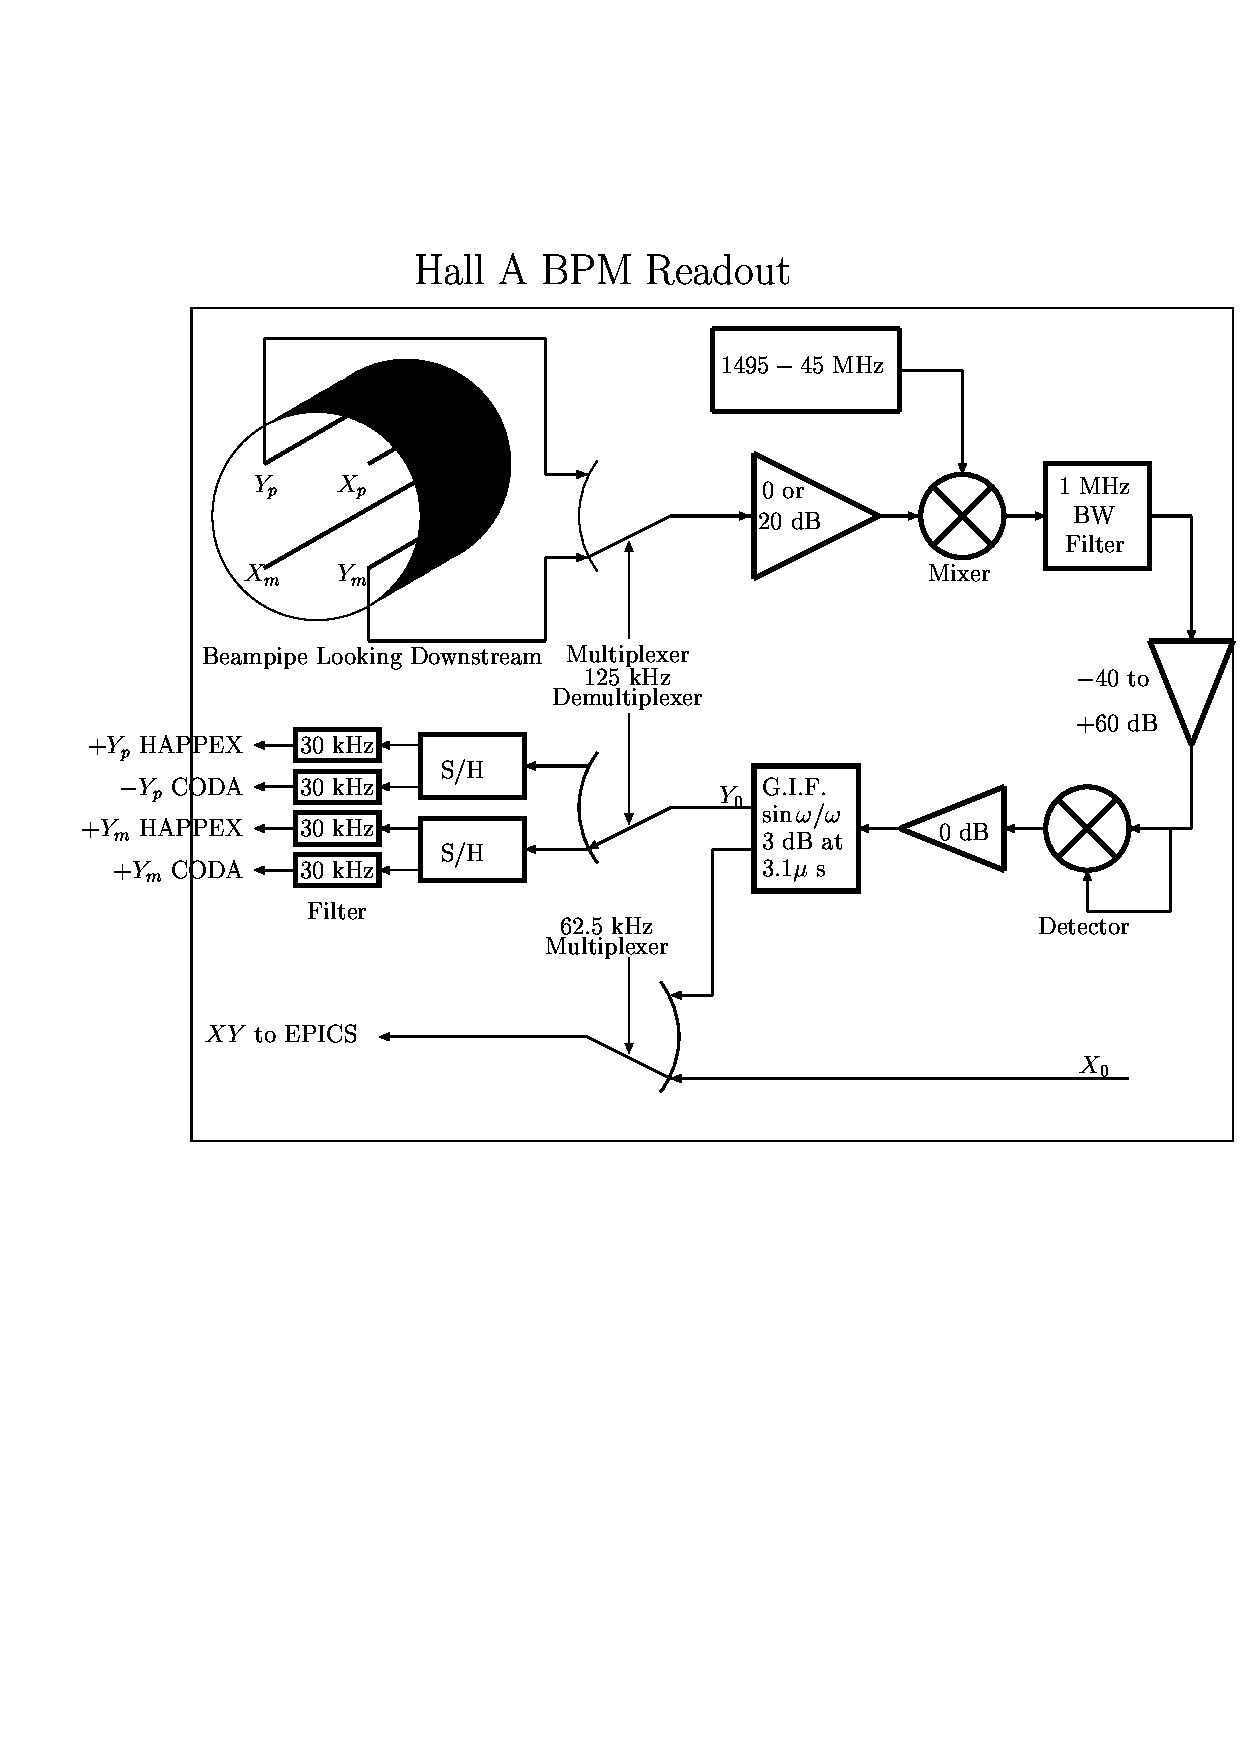
\includegraphics[angle=0,width=15cm]{BPM_fig}
{\linespread{1.}
\caption[Beamline: BPM Readout Electronics]{Schematic of the BPM readout
electronics}
\label{fig:bpmel}}
\end{center}
\end{figure}
}

1. The averaged position over 0.3 seconds is logged into the EPICS~\cite{EPICSwww} database (1 
Hz updating frequency) and injected into the datastream every 3-4 seconds, 
unsynchronized but with an orientative timestamp. From these values we can 
consider that we know the average position of the beam calculated in the EPICS 
coordinate system which is left handed.

2. Approximately once a shift (or more often if requested by the experimenters) 
a B-scope procedure ~\cite{bi:TP} can be performed using the same EPICS electronics 
which then gives the peak-to-peak variation of the beam.

3. Event-by-event information from the BPMs are recorded in the CODA datastream
from each of the 8 BPM antennas (2x4) from which the position of the beam can be 
reconstructed. However, these raw values belong to a parallel electronics chain 
whose constants have to be retrieved by calibrations to the EPICS or scanner 
data. 

\subsection{Beam Exit Channel}

After the target vacuum chamber, which was built by
the University of Virginia, there is an exit beam pipe which 
transfers the scattered beam onto the dump tunnel under vacuum. This exit beam 
pipe is made of a thin walled aluminum spiral corrugated pipe of welded 
construction. The largest diameter is 36 inches with a 0.164 inches wall 
thickness and the smallest diameter is 6 inches with a 0.042 inches wall 
thickness. The whole assembly is rather light (approximately 800 kg) and is 
supported by H shaped adjustable stands. To prevent possible linear collapse 
of the larger diameter sections under vacuum load, four aluminum channels of 
total cross-sectional area of 3'' are welded to its side. A vacuum of 
10$^{-5}$ Torr is maintained with a turbomolecular pump. The exit face of this 
pipe has a 12'' port and is connected to the diffuser with a Beryllium 
window.

}

\section{ Machine/Beamline protection system}
\label{sec:beam-fsd}

The MPS~\cite{MPScebaf} system is composed of the Fast Shutdown System (FSD), Beam Loss 
Monitor (BLM), and gun control system.

The FSD system is a network of permissive signals which terminate at the 
electron gun and chopper 1. The permissive to the gun and chopper
1 may be inhibited by any device connected to an FSD mode. Devices connected to the 
FSD system include vacuum valves, RF systems, Beam loss systems, beam current 
monitors, beam dumps, and particular to Hall A, the target motion mechanism 
and the raster (value and derivative).

The gun control system includes software program which monitors beam 
operating conditions and the state of the FSD and BLM systems. the program 
will warn the operators if a potential for beam damage exists. Potential for 
damage exists when running high average current beam, when FSD nodes are 
masked and when the beam power approaches the operating envelope limits for a 
specific beam dump.

\clearpage
\begin{safetyen}{10}{10}
\section{Safety Information}
\end{safetyen}
}
%
% Information for the ESAD
%

\begin{safetyen}{0}{0}

The beamline in the Hall provide the interface between the CEBAF accelerator
and the experimental hall.   All work on the beamline must be coordinated 
with both physics division and accelerator division; in order to ensure
safe and reliable transport of the electron beam to the dump.

\subsection{Hazards and Mitigations}

All magnets (dipoles, quadrupoles, sextupoles, beam correctors) and beam 
diagnostic devices (BPMs, scanners, Beam Loss Monitor, viewers) necessary for 
the transport of the beam are controlled by Machine Control Center (MCC) 
through EPICS~\cite{EPICSwww}, except for special elements which are addressed in the 
subsequent sections. The detailed safety operational procedures for the Hall 
A beamline should be essentially the same as the one for the CEBAF machine 
and beamline.\\ 

  
\noindent{}Personnel who need to work near or around the beamline should keep in mind the potential hazards:
\begin{itemize}
  \item Radiation ``Hot Spots'' - marked by ARM or RadCon personnel,
  \item Vacuum in the beam line tubes and other vessels,
  \item Thin windowed vacuum enclosers (e.g. the scattering chamber),
  \item Electric power hazards in vicinity of the magnets,
  \item Magnetic field hazards in vicinity of the magnets, and
  \item Conventional hazards (fall hazard, crane hazard etc.).
\end{itemize}

The most hazardous areas along the beamline are roped off it restrict access.   
In particule the scattering chamber, with it's large
volume and thin windows requires hearing protection once it has been evacuated.   
Signs are posted by radcon for any hot spots along the beamline and
radcon must be notified before work is done in a posted area.

Some magnets, as the M{\o}ller spectrometer elements, are covered with plastic
sheets for electric safety. Any access to these magnets requires
the ``Lock and Tag'' procedure~\cite{EHScebaf} and the appropriate training,
including the equipment-specific one. \\

\noindent{}Additional safety information is available in the following documents:
\begin{list}{--}{\setlength{\itemsep}{-0.15cm}}
  \item EH\&S Manual~\cite{EHScebaf};
  \item PSS Description Document~\cite{PSScebaf}
  \item Accelerator Operations Directive~\cite{AODcebaf};
\end{list}

\subsection{Responsible Personnel}

Since the beamline requires both accelerator and physics personnal to maintain
and operate and it is very important that both groups stay in contact that any 
work on the Hall A beamline is coordinated.

\begin{namestab}{tab:beam:personnel}{Beam line: authorized personnel}{%
   Beamline physics division and accelerator divison points-of-contact.}
  \namestabheader{Hall A Physicists}
  \DouglasHiginbotham{\em 1st Contact}
  \RobertMichaels{\em 2nd Contact}
  \namestabheader{Liaisons from Accelerator Division}
  \HariAreti{..to Physics}
  \YvesRoblin{..to Hall-A}
\end{namestab}
\end{safetyen}


\newpage
\section{ Beam Position Monitors}

To determine the position and the direction of the beam on the experimental 
target point, two Beam Position Monitors (BPMs) are located at distances 7.524 m 
(IPM1H03A) and 1.286 m (IPM1H03B) upstream of the target position. 
The BPMs consist of a 4-wire antenna array of open ended thin wire striplines 
tuned to the fundamental RF frequency of 1.497 GHz of the beam ~\cite{bi:bar90}. The 
standard difference-over-sum technique is then used ~\cite{bi:HW} to determine the 
relative position of the beam to within 100 microns for currents
above 1 $\mu $A. The absolute  position of the BPMs can be calibrated with respect to the 
scanners (superharps) which are located adjacent to each of the BPMs (IHA1H03A 
at 7.353 m and IHA1H03B at 1.122 m upstream of the target). The schematic of the 
readout electronics is shown in Figure ~\ref{fig:bpmel}. The
position information from the 
BPMs can be recorded in three different ways:

\begin{figure}
\begin{center}
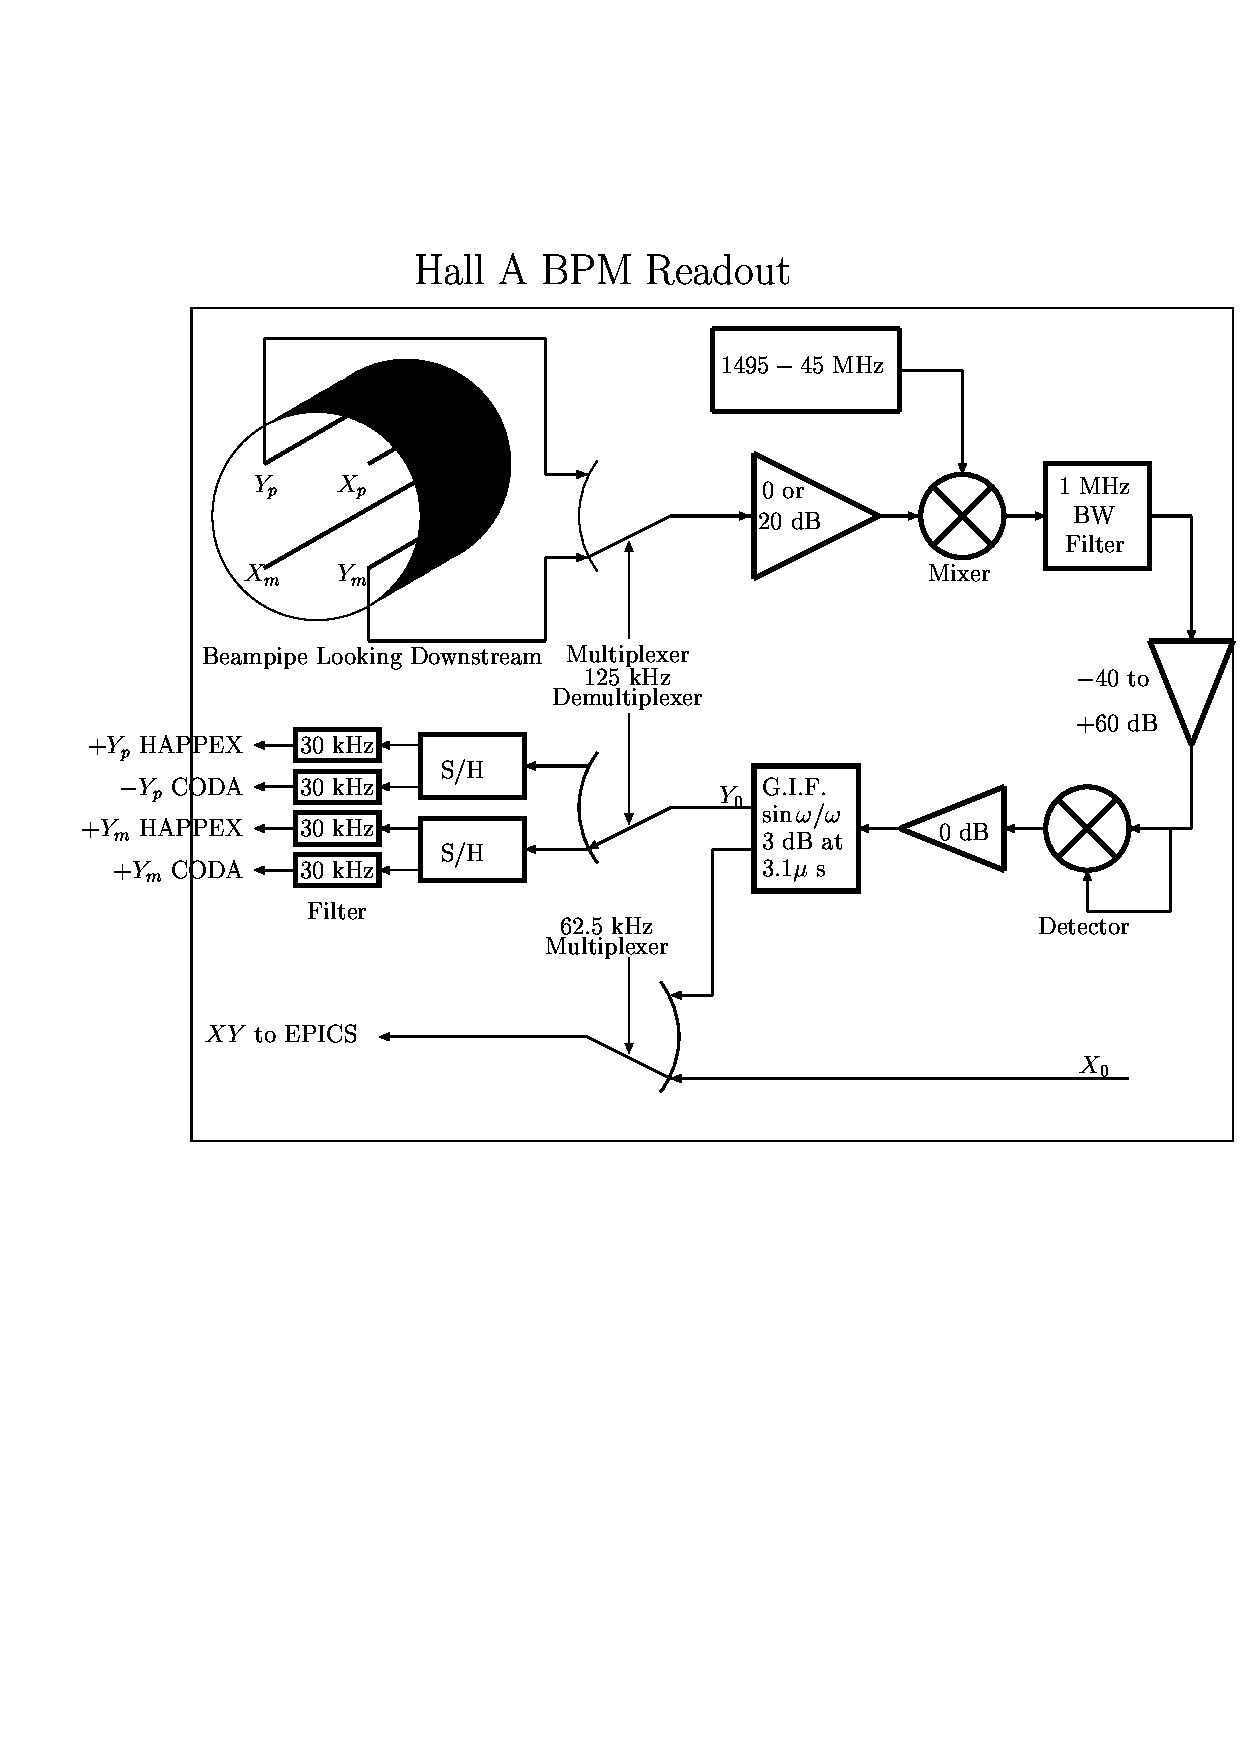
\includegraphics[angle=0,width=15cm]{BPM_fig}
{\linespread{1.}
\caption[Beamline: BPM Readout Electronics]{Schematic of the BPM readout
electronics}
\label{fig:bpmel}}
\end{center}
\end{figure}

\vskip 0.5cm

1. The averaged position over 0.3 seconds is logged into the EPICS database (1 
Hz updating frequency) and injected into the datastream every 3-4 seconds, 
unsynchronized but with an orientative timestamp. From these values we can 
consider that we know the average position of the beam calculated in the EPICS 
coordinate system which is left handed.

\vskip 0.5cm

2. Approximately once a shift (or more often if requested by the experimenters) 
a B-scope procedure ~\cite{bi:TP} can be performed using the same EPICS electronics 
which then gives the peak-to-peak variation of the beam.

\vskip 0.5cm

3. Event-by-event information from the BPMs are recorded in the CODA datastream
from each of the 8 BPM antennas (2x4) from which the position of the beam can be 
reconstructed. However, these raw values belong to a parallel electronics chain 
whose constants have to be retrieved by calibrations to the EPICS or scanner 
data. 


%\begin{thebibliography}{99}
%\bibitem{bi:bar90} W. Barry et al., CEBAF-PR-90-009 (1990).
%\bibitem{bi:HW} C. Hyde-Wright et al., Beam Position Studies for E93050 and priv. comm..
%\bibitem{bi:TP} T. Powers, priv.  comm.. 
%\end{thebibliography}
% ===========  CVS info
% $Header: /group/halla/analysis/cvs/tex/osp/src/beamline/bpms.tex,v 1.1 2003/06/05 17:28:32 gen Exp $
% $Id: bpms.tex,v 1.1 2003/06/05 17:28:32 gen Exp $
% $Author: gen $
% $Date: 2003/06/05 17:28:32 $
% $Name:  $
% $Locker:  $
% $Log: bpms.tex,v $
% Revision 1.1  2003/06/05 17:28:32  gen
% Initial revision
%

\newpage
\section[Beam Current Measurement]{Beam Current Measurement
\footnote{
  $CVS~revision~ $Id: bcm.tex,v 1.5 2003/12/13 06:23:37 gen Exp $ $
}
\footnote{Authors: A.Saha \email{saha@jlab.org}}
}

The Beam Current Monitor (BCM) is designed for stable, low noise, non-intercepting 
beam current measurements. It consists of an Unser monitor, two rf cavities, 
the electronics and a data acquisition system. The cavities and the Unser monitor 
are enclosed in a box to improve magnetic shielding and temperature stabilization.
The box is located 25 m upstream of the target. You can recognize it as a grey 
object on the stands, about 2 m downstream from where the beam enters the 
hall. 

The DC 200 down-converters and the Unser front end electronics are located in Hall 
A. The temperature controller, the Unser back end electronics and its calibration 
current source, cavity's RF unit (housing the RMS-to-DC converter board) and all 
multi-meters, VME crate and computers are located in Hall A control room.

\infolevone{
\subsection{ System Layout}

The schematic diagram of the BCM system is presented in
Fig.~\ref{fig:halla_bcm}.
\begin{figure}[htp]
\begin{center}
\includegraphics[angle=0,width=0.9\textwidth,clip]{habcm_r}
{\linespread{1.}
\caption[Beam Current Measurement: Schematic]{Schematic of the Hall A beam
current measurement system.}
\label{fig:halla_bcm}}
\end{center}
\end{figure}

The Unser monitor is a Parametric Current Transformer designed for non-destructive 
beam current measurement and providing an absolute reference. The monitor is 
calibrated by passing a known current through a wire inside the beam pipe and has a 
nominal output of 4 mV/$\mu $A. It requires extensive magnetic shielding and 
temperature stabilization to reduce noise and zero drift. As the Unser monitor's 
output signal drifts significantly on a time scale of several minutes, it cannot be 
used to continuously monitor the beam current. However, this drift is measured 
during the calibration runs (by taking a zero current reading) and removed in 
calibrating the cavities.  The more stable cavities are then used to determine the 
beam current and charge for each run. We also use the OLO2 Cavity Monitor and the 
Faraday Cup 2 at the Injector section to provide an absolute reference during 
calibration runs.

The two resonant rf cavity monitors on either side of the Unser Monitor are 
stainless steel cylindrical high Q ($\sim 3000$) waveguides which are tuned to the 
frequency of the beam (1.497 GHz) resulting in voltage levels at their   outputs 
which are proportional to the beam current. Each of the rf output signals from the 
two cavities are split into two parts. One part of the signal is  converted to 10 
kHz signals (by the ``downconverters'') and fed into an RMS-to-DC converter board 
consisting of a 50 kHz bandpass filter to  eliminate noise, amplified and split to 
two sets of outputs, which after further processing are recorded in the data 
stream. These two paths to the data stream (leading to the sampled and integrated
data ) will now be described. (The other part of the split signal is downconverted 
to 1 MHz signals and represents the old system (pre Jan 99). Only the HAPPEX 
collaboration presently uses these signals.)

For the sampled (or EPICS~\cite{EPICSwww} or Slow) data, one of the amplifier outputs is sent to a 
high precision digital AC voltmeter (HP 3458A). Each second this device provides 
a digital output which represents the  RMS average of the input signal during that 
second.  The resulting number is  proportional to the beam charge accumulated 
during the corresponding second (or, equivalently, the average  beam current  for 
that second). Signals from both cavity's multi-meters, as well as from the 
multi-meter connected to the Unser, are transported through GPIB ports to the HAC 
computer where they are recorded every 1 to 2 seconds via the data-logging process 
which is described in the calibration procedure. They are also sent through EPICS 
to CODA and the data stream where they are recorded at  quasi-regular intervals, 
typically every two to five  seconds.

For the integrated (or VTOF or Fast) data, the other amplifier output is sent to an 
RMS-to-DC converter which   produces  an analog DC  voltage  level. This level 
drives a Voltage-To-Frequency (VTOF) converter whose output frequency is  
proportional to the  input DC voltage level. These signals are then fed to Fastbus  
scalers and are finally injected into the data stream along  with the other scaler 
information.  These scalers simply accumulate during  the run, resulting  in a 
number which is proportional to the time integrated voltage level and therefore 
more accurately represents the true integral of the current and hence the total 
beam charge. The regular RMS to DC output is linear for currents
from about 5 $\mu$A to somewhere well above 200 $\mu$A.
 Since it is non-linear at the lower 
currents, we have introduced a set of amplifiers with differing gains (x3 and x10) 
allowing the non-linear region to be extended to lower currents at the expense of 
saturation at the very high currents. Hence there are 3 signals coming 
from each BCM (Upx1, Upx3, Upx10, Dnx1, Dnx3, Dnx10). All 6 signals are fed 
to scaler inputs of each spectrometer (E-arm and H-arm) . Hence we have a 
redundancy of 12 scaler outputs for determining the charge during a run. During 
calibration runs we calibrate each of these scaler outputs.   
}

\begin{safetyen}{10}{10}
\subsection{ Authorized Personnel}
\end{safetyen}

All Hall A members are authorized to take BCM calibration data using the Standard 
Non-Invasive Hall A BCM Calibration Procedure. The extended calibration procedures 
involving the Faraday Cup 2 and the OLO2 monitor at the Injector are presently 
performed by A. Saha. 

\vskip 0.2cm

The Accelerator AES group performs the maintenance of the BCM monitors. These 
include:

\begin{tabular}{l l}
1. The Unser calibration. & Every 3 months \\
2. Resonant Cavities Tuning. & Every Downtime \\
3. Multi-meters Autocalibration. & Every Downtime \\
4. Connectors Cleaning. &  Every year \\
5. Unser Keithley Current Source. & Calibration Yearly \\
6. Digital Multi-meters HP3458A and HP 34401A. & Calibration Yearly\\   
\end{tabular}

System Contacts are shown in Table~\ref{tab:BCM:personnel}.
\begin{namestab}{tab:BCM:personnel}{BCM: authorized personnel}{%
   Beam Current Monitor: authorized personnel}
  \ArunSaha{\em Contact}
  \JohnMusson{Accel. expert}
\end{namestab}
%Jean-Claude Denard -x 7555




% ===========  CVS info
% $Header: /group/halla/analysis/cvs/tex/osp/src/beamline/bcm.tex,v 1.5 2003/12/13 06:23:37 gen Exp $
% $Id: bcm.tex,v 1.5 2003/12/13 06:23:37 gen Exp $
% $Author: gen $
% $Date: 2003/12/13 06:23:37 $
% $Name:  $
% $Locker:  $
% $Log: bcm.tex,v $
% Revision 1.5  2003/12/13 06:23:37  gen
% Septum added. Name tables. Polishing
%
% Revision 1.4  2003/12/05 05:48:30  gen
% Polishing
%
% Revision 1.3  2003/06/06 15:19:02  gen
% Revision printout changed
%
% Revision 1.2  2003/06/05 23:29:59  gen
% Revision ID is printed in TeX
%
% Revision 1.1.1.1  2003/06/05 17:28:32  gen
% Imported from /home/gen/tex/OSP
%
%  Revision parameters to appear on the output

\newpage
\section[Fast Raster]{Fast Raster
\footnote{Authors: R.~Michaels \email{rom@jlab.org}}
}


The beam is rastered on target with an amplitude of
several millimeters at 25 kHz to prevent overheating.  
The raster is a set of four of air-core dipoles located
approximately 23 m upstream of the target. 
Two dipoles are for horizontal (X) motion and
another two for vertical (Y).  During the 6 GeV era
there was only one pair of X and Y, but we have doubled
the raster to account for the energy increase to 11 GeV.
The arrangement along the beamline along the 
direction of the beam will be XXYY.

For a typical 40A current in the raster coils, the
deflection by one pair (e.g. the X direction) of coils, 
in radians, is $\theta = 1.94 \times 10^{-3}/ E$
where $E$ is the electron's energy in GeV.
For example, at $E = 6$ GeV, a 0.32 mrad deflection is achieved.
Projected onto the target (about 21 m away) this is a $\pm$ 6.8 mm
excursion {\it if} there were no other magnetic fields 
between the raster and the target; however, there are quadrupoles
which change this depending on the beam tune.

Since 2003 we've used the triangle-wave 
raster pattern designed by Chen Yan.  
This achieves a very uniform rectangular
density distribution of beam on the target 
by moving the beam with a time-varying dipole
magnetic field whose waveform is triangular
with very little dwell time at the peaks.  
The electronics design is an ``H-bridge''
in which switches are opened and closed 
at 25 kHz, to switch between two directions 
of current (100 A peak-to-peak) 
through the raster coils.

Three new features during the 12-GeV era are 
1) the driver of the H-bridge electronics is now
an Agilent model 33522A waveform generator; and
2) The two X are synchronized with each other, and
the two Y are synchronized.  This makes the kicks
add and allows us to accomodate the higher energy
of the beam; and 3) The entire raster can
be synchronized to an external 10 MHz wavetrain
supplied by the polarized injector electronics.
This makes the nominal 25 kHz an exact multiple of
the helicity-flip rate, which achieves a cancellation
of raster noise, important for parity-violation 
experiments only.
The syncrhronization of the pairs of X and Y are
accurate to within a few nsec.

For most users, these three new features will not be
noticeable and the raster will appear to function
the same as during the 6 GeV running.
A user can view the 
status of the raster in the
EPICS overview screen called ``General Accelerator
Parameters'' where the set-point for the radius amplitude
and the readback of the peak-current in the raster are displayed.

Control of the raster is done by first asking the MCC
operators to set up the raster for a particular size
typically 2 mm square.
The control software assumes a field-free region between
the raster and the target, so it is only approximately
correct because there are several quadrupoles in this region.
It is important to check the raster spot size and
make adjustments if necessary.  The adjustment is made
by asking MCC to change the size and noting the 
linear relationship between what their software says
the size is and the actual size.
Relatively small independent adjustments to the 
gains on the X and the Y raster
coils are available in the middle room of the hall A
counting room using the ``PGA Controller'' knobs;
however, it is not recommended to touch these.
Near these knobs is also located an oscilloscope X-Y trace
of the current in the raster.  A fast shutdown (FSD) shuts
the beam down within 0.1 msec if the raster fails, thus
affording some protection of the target.

{\it NOTE:  If you are unsure of the status of the raster,
measure the spot size with very low current ($\le 2 \mu$A) or with
the target out of the beam.}  It would be a mistake
to check the beam spot size with high current on target; by
the time you check it, the target may already be destroyed.
The rastered beam spot on target can be checked with
plots in the ROOT analyzer or by 
using the stand alone code called \mycomp{spot},
also called \mycomp{raster}.
For more details on usage, type \mycomp{spot -h} (help)
on the ADAQ computers.

Regarding the BPM measurements, it should be noted that 
the stripline BPMs displayed by \mycomp{spot} have a high-frequency 
cutoff of approximately 30 kHz.  Since the raster frequency is 25 kHz
the plot of the amplitude distribution shows spikes at the 
limits of the orbit, instead of a flat distribution.  The scale
factor between what is seen in \mycomp{spot} and the real width of the beam
is $\sim 1.5$, i.e. the beam is 1.5 times bigger than the naive
reading of the \mycomp{spot} distribution.



\newpage
% Updated Comments Dec. 2
\infolevone{
\chapter[Arc Energy Measurement]{Arc Energy Measurement
\footnote{Authors: D. Higinbotham \email{doug@jlab.org}}
}
}

\infoleveqnull{
\section{Arc Energy Measurement}
\subsection{Overview}
In order to determine the integral field of the eight dipoles that lead to Hall A, and 
in turn determine the beam energy, a nineth dipole wired in series with the rest is 
located in a special shed near the hall A counting house.
}

\infolevone{
The ARC energy measurement is under EPICS~\cite{EPICSwww} control through 
a MEDM~\cite{MEDMwww} display. Two
independent control systems are used: the beam bend angle measurement through
the arc ("scanners") and the field integral of
the arc ("integral"). To measure the energy: 

\begin{itemize}
\item perform several angle measurements 
\item perform an integral measurement 
\item analyze the integral measurement and note the value of the arc field 
integral 
\item analyze the angle measurements, average the results (proposed by the 
software),
then ask for the energy calculation, enter the above arc field integral and
you will get the beam energy computed from the average angle. 
\end{itemize}

\section{Summary of ARC operations }

Six scanners of the same type, called ``ARC scanner'' and labelled
from scanner \#1 to \#6, are installed on the Hall-A beamline. Scanners \#1
to \#4 are used for the ARC energy measurement and they are located on the Hall-A
arc: \#1 [1HA1C07A] and \#2 [1HA1C07B] just upstream of the arc, in the BSY, and 
\#3 
[1HA1C18A] and \#4 [1HA1C18B] in the Hall-A
tunnel, just upstream the Compton polarimeter. Scanners \#5 [1HA1H03A] and \#6 
[1HA1H03B] 
are located
between the Moller and the target to control the beam geometry on the target
and their use will not be discussed here. 

Procedure for running a harp scan is described elsewhere\footnote{
Harp scan procedure \url{http://hallaweb.jlab.org/equipment/beam/harp_halla/harp.html}.}

Each scanner has a motor/ball-screw/shaft-encoder/vacuum-penetrator system moving
accurately a set of 3 tungsten wires through the beam. Each time a wire crosses
the beam a PMT located a few meters downstream records a signal due to the 
electromagnetic
shower induced by the beam in the wire. Both forward and backward passes are
recorded. The motion is a horizontal translation and, for a forward pass: 

-the translation is from beam left to beam right, 

-the two first wire crossing the beam are at 45deg from the vertical, 

-the third wire, which is the only important for the ARC energy measurement,
is vertical. 

Recording, during the scan, the scanner position and the PMT output voltage
allows us to determine the beam position at each scanner location. Then, using
calibration data not detailed here, we deduce the net beam bend angle through
the arc. This result measured in dispersive arc tuning, along with the field
integral of the arc dipoles, provides an accurate determination of the beam
energy. 

\vspace{0.3cm}

\section{Summary of field integral }

The purpose is to measure absolutely the straight field integral of a 
"BA"
3m long dipole, called the "9th dipole" and located in the
"Dipole Shed". It is of the same type as the 8 arc dipoles
and is powered in series with them. 

The ARC integral setup is basically made of a 3m long plate (the 
"probe")
which is able to move inside the 9th dipole gap along the beam axis and carrying 
two
field measurement devices: a pair of pick-up coils connected in series and a
set of NMR probes. The coils are on both ends of the probe and the NMRs close
to the center. 

-at the "upstream" probe position, the 
"downstream"
coil is close to the dipole center, the "upstream" is outside
the dipole and the NMRs at one end of the dipole: 

Door$<-$-- ....................$<-$-------DIPOLE-----$--->$ 

.............$<-$-------PROBE------$--->$ 

-at the "central" probe position, each coil is at one end
of the 3m long dipole and the NMRs close to the dipole center: 

Door$<-$-- ...................$<-$-------DIPOLE-----$--->$ 

..................................$<-$-------PROBE------$--->$ 

-at the "downstream" probe position, the 
"upstream"
coil is close to the dipole center, the "downstream" is outside
the dipole and the NMRs at one end of the dipole: 

Door$<-$-- ...................$<-$-------DIPOLE-----$--->$ 

....................................................$<-$-------PROBE------$--->$ 

We call upstream the position where the probe is the closest to the shed access
door. Among the 3 above positions, the only one where the NMR can lock on the 
dipole
field is the central one as in the extreme position of the probe, the field 
homogeneity
is not sufficient. The probe position is controlled by a linear encoder. The
Z axis refers to the "beam" direction, increasing from upstream
to downstream. We use three kinds of "Z": 

-Zm to locate a point inside the magnet. The dipole center is at Zm=0 and the
yoke ends at +-1500.mm 

-Zp to locate a point inside the probe. The probe center is at Zp=0. Each of
the 4 NMR probes has a Zp given in the file "magnet.dir".
At a temperature of 21C, the coils are at Zp=+-1519.815mm (from magnet.dir) 

-Zd to refer to a displacement of the probe w.r.t. the dipole. Zd=0 refers to
the upstream (home) position of the probe. The integral measurement is performed
from Zd=0.000mm (1st PDI trigger) to Zd=3199.000mm (last PDI trigger), for forward
pass. Zd is given by the display (at the top of the rack) or by the master screen
("OUT"). 

The relationship between Zm, Zp and Zd is: 

Zd-Zm+Zp=C 

where C is a constant given in magnet.dir (C=1604.000 nomin.). Example of use:
to have the probe center at the dipole center, one must set Zd=1604.000mm (set
Zm=0 and Zp=0 in the above formula, and solve for Zd) 

The integral measurement sequence is the following: 

-from the current position (a priori arbitrary) move the probe upstream, up
to a limit (optic) switch. 

-move downstream by a few mm to cross the encoder index (encoder initialization) 

-move to the central position to measure the central field by NMR, the system
checks if the NMR locks and if the reading is stable, it will be the 
"before"
field 

-move back to upstream position 

-move to downstream position while integrating the flux through the coil system,
this measurement will be called the "forward" integral (duration
\( \sim  \) 7s) 

-move back to upstream position while integrating the flux through the coil
system, this measurement will be called the "backward" integral
(duration \( \sim  \)7s) 

-move to the central position to measure the central field by NMR, the system
checks if the NMR locks and if the reading is stable, it will be the 
"after"
field. 

In addition to the central field, 4 probe temperatures, a local excitation current
measurement, the setting of the dipoles P.S, the readback of the dipoles P.S
and the probe position at NMR measurement time are recorded 
"before"
and "after". 

To perform an integral field measurement: 

1-check if the system works (see "details on integral system 
check"
below) 

2-run the above integral sequence (see "details on integral run"
below) 

3-fix the error(s) if any (see "details on integral errors"
below) 

4-save the data in a file (see "details on integral data save"
below) 

5-analyze the data  


\section{Details on integral run }

To run the integral measurement sequence, call the 
\mycomp{arc\_integral.adl}
medm screen, then: 

-push "start" to start the full sequence 

-look at the results displayed: 

-after the "before" NMR measurement: the 
"before"
data set 

-after the "forward" integral pass: the forward velocity profile
and the forward voltage-after-gain profile 

-after the "backward" integral pass: the backward velocity
profile and the backward voltage-after-gain profile 

-after the "after" NMR measurement: the 
"after"
data set 

-if "BAD NMR" or "PDI saturation" flags
are set, or if something is obviously wrong in the data or plots, call expert. 

-data are ready to be saved (see "Details on integral data save"
below) 


\section{Details on temperatures }

The AC system of the shed is made of two cooling units, a heating unit and a
controller connected to two temperature sensors : one located in the shed and
one located in the BSY. This system is programmed in such a way that the 
temperature
of the shed follows the BSY temperature within +-2C. The BSY temperature can
be anywhere in the 18C to 35C range, regardless of the season. The BSY 
temperature
and the shed temperature are given (in F) by a display panel located close to
the workstation, on the wall. The AC system can be set in manual control by
turning from "auto" to "manual" a set of
switches controlling the cooling units and the heater unit. These switch boxes
are located on the shed wall. If the shed temperature is above 34.4C (94F),
call the crew chief (the electronics can be damaged) and cool down the shed in manual
AC mode. The 4 temperature sensors of the probe are labelled Tx+z+, Tx+z-, Tx-z+,
Tx-z- depending on their position w.r.t. the frame. 

Both "x+" sensors are on the probe edge which is inside the
dipole gap and both "x-" sensors on the opposite edge which
is outside the dipole gap. Both "z-" sensors are at 1/4 of
the long dimension of the probe and both z+ at 3/4 of this length. The average
of the 4 temperatures is used by the analysis program to correct the coil distance
from the thermal expansion of the probe, so it is important to make sure that
the 4 sensors are working well. The user can just make sure that the temperatures
displayed in \mycomp{arc-master.adl} or recorded in 
\mycomp{arc-integral.adl}
are realistic. In \mycomp{arc-integral.adl} they are given in the
order: Tx+z-, Tx+z+, Tx-z-, Tx-z+ Tx-z- and Tx-z+ should be close to the shed
temperature. Tx+z- and Tx+z+ depend on the probe position, as the gap (iron
yoke) is warmer than the shed and the dipole coil (at both ends of the dipole)
is warmer than the iron yoke. For a probe in a central position for more than
about one hour, the Tx+z- and Tx+z+ sensors should give the yoke temperature,
i.e the shed temperature plus 0. to 5.C, depending on the current, LCW temperature
and the magnet/shed temperature history. The 4 temperatures are also displayed
inside the shed, on the electronics rack. These values are digitized by separate
ADCs, so they may differ from the remote values by \( \sim  \)0.1C. 
}

\begin{safetyen}{10}{10}
\infolevone{\section{Shed access and safety }}

Due to the the dipole magnet and motion system, the access to the shed is limited to authorized
persons which are listed in the ESAD and listed below. To be added to the list, 
contact Douglas Higinbotham.
The standard
operation mode of the integral measurement setup is the remote mode, through
the network, from the counting house.
\end{safetyen}

\begin{safetyen}{10}{10}
\infolevone{\section{List of Authorized Personnel for Shed Access}}
\infoleveqnull{\subsection{List of Authorized Personnel for Shed Access}}
\end{safetyen}
\begin{namestab}{tab:arc:personnel}{Arc Energy Measurement: authorized personnel}{%
                 Arc Energy Measurement: authorized personnel}
  \namestabheader{Hall A Personnel}
  \DouglasHiginbotham{\em Contact}
  \namestabheader{Accelerator Personnel}
  \MichaelTiefenback{}
  \YvesRoblin{}
  \RickGonzales{}
  \BillMerz{}
  \MarkAugustine{}
  \HariAreti{}
  \PeteFrancis{}
  \ScottHiggins{}
  \DavidSeidman{}
  \RonLauze{}
  \TonyDay{}
  \ChristopherCurtis{Alignment group}
  \namestabheader{CEA - Saclay experts}
  \PascalVernin{}
  \ChristianVeyssiere{}
  \FrancoisGougnaud{}
  \JacquesMarroncle{}
\end{namestab}



\newpage
\infolevone{
\chapter[Target Chamber]{Target Chamber
\label{sec:target_chamb}
\footnote{
  $CVS~revision~ $Id: tgtcham.tex,v 1.11 2005/04/04 22:27:25 gen Exp $ $
}
\footnote{Authors: ?? \email{??@jlab.org}}
}

The cryo-targets and the waterfall targets 
(see Sec.~\ref{sec:targets-overv}) 
are contained in a special target chamber which is a large 
evacuated  multistaged can. So far, three chambers have been designed:
\begin{list}{\arabic{enumi}.~}{\usecounter{enumi}\setlength{\itemsep}{-0.15cm}}
  \item a chamber used up to 2003;
  \item a chamber designed for use with septum magnets, starting in 2003;
  \item a chamber designed for use with the BigBite spectrometer.
%\footnote{
%        No yet manufactured by Dec,2003.}.
\end{list}

Here, chamber 1 is described. Chambers 2 and 3 are only different in 
size and slightly in shape. The safety considerations fully apply to chambers 2 and 3.
The chamber was designed to isolate the beam line vacuum from  each
HRS so that each HRS could rotate
around the target without vacuum coupling and without jeopardizing
certain desired kinematic and acceptance  specifications of 
both high resolution spectrometers
needed for approved experiments.  It  was also designed to simultaneously
 contain a liquid or gas target and an array of water cooled thin
 metallic foils, both remotely controlled and also be adaptable for
the waterfall target. The desired kinematic specifications that were
 considered included momentum and energy resolution in both arms,
 angular range of spectrometers, angular acceptance, and luminosity.
The chamber vacuum is isolated from the  HRS by using thin aluminum foils. 

The target chamber is designed so that
each spectrometer will have continuous coverage in the standard tune from
$\theta_{min}=$12.54$^\circ$ to $\theta_{max}=$165$^\circ$.
The aluminum window is 6~$in$ high and 0.016~$in$ thick made of 5052 H34 aluminum foil.
The foil forms regularly spaced vertical ridges when
placed under load. The window had an inter-ridge
spacing of 3 inches.
If the window is treated as a collection
of smaller rectangular windows which have the full vertical height
of 6 inches and the inter-ridge spacing as a width,
then stress formulas predict that the 0.016 $in$
material would reach ultimate stress at a pressure higher than 35 PSID
(for both over-pressure and under-pressure). 
There is a gate valve between the 
scattering chamber and the beam entrance (exit) 
pipe. Both 
valves will be closed automatically in the
event that the chamber vacuum begins to rise and an FSD will be caused
( this is done via a relay output of the scattering
chamber vacuum gauge). If either valve is closed an FSD will result.

The target chamber is supported by a 24 $in$ diameter pivot post
secured in concrete, rising about 93.6 $in$ above the Hall A cement floor.
The Hall A target chamber
consists of an aluminum middle ring, a stainless steel base ring,
each with a 41.0 $in$ inner diameter,
and a stainless steel cylindrical top hat with 40 $in$ inner diameter
to enclose the cryotarget and secure the cryogenic connections.

When the scattering chamber is under vacuum, there is a potential
danger of window rupture.
The loud noise from the rupture could hurt
one's ears if not protected. Therefore when the chamber is under vacuum,
protective covers are put on if possible. These must be taken off
for data taking. For restricted access, the protective cover is required
to be on when the chamber is under vacuum. Before switching from controlled
access to restricted access, the protective cover is required to be installed.
Anytime that the scattering chamber
is under vacuum, the pivot area is enclosed in a rope or tape barrier
and a warning sign is posted.
Hearing protection is required in the enclosed area.

\infolevone{
	The aluminum ring with an outer diameter of 45.0 $in$ and
wall thickness 2.0 $in$  is necessary for a sturdy support structure and
to permit machining of the outside surface to accommodate
the flanges for fixed and sliding seals mounted on
opposite sides of the ring that vacuum connect the chamber to each HRS.
The height of the aluminum ring shown is 36.0 $in$, which is
designed to accommodate the mounting flanges.
The stainless steel base ring 
is 11.50 $in$ in height with
one pump-out 6 $in$ diameter port  and with
seven 4 $in$ viewing and electrical feed-through ports.
The base ring will also contain support mechanisms for the solid
target ladder assembly, a rotisserie for collimating slits, radiators, and
magnetic
fingers for
removing the solid target vacuum-lock can. The total height of the top
ring, middle ring, and
base ring is 93.81 $in$. This length is partly determined by our desire to
include with the cryogenic extended target a solid target vertical ladder
secured in an inverted hat through a hole in the base of the chamber.

	The base ring includes an end plate through which the
inverted hat will be adapted to fit into the large vertical pipe serving
as the pivot post for the Hall A spectrometers.

	The stainless steel cylindrical top hat  has
40.0 $in$ inner diameter, and is 0.375 $in$ thick and
46.31 $in$ high , which is necessary to permit the
cryotarget to be withdrawn and to make space available to expose the solid
targets to the electron beam.

   The 200 $\mu$A electron beam, focused to a $\sim$\(0.1\, mm\times
0.1\) mm spot and rastered $\pm$5 mm horizontally or vertically on the
target, enters through a oval hole in the middle ring which
is 2.06 $in$ wide and exits through a 1.81 $in$ hole connected to the
exit pipe.
}

\infolevone{
\section{Target Chamber - Spectrometer Coupling}

   The aluminum middle ring will support a flange on each side for each high
resolution spectrometer. Four flanges will be available: Two flanges will
contain a 6 $in$ window opening which will be covered with a thin foil
(e.g., 10 mil aluminum) .
These two flanges will be used for experiments utilizing
extended  targets that do not require optimum momentum resolution.
The other two flanges will have two fixed ports (with a 8 $in$ $\times$ 6 $in$
opening)
which will be mainly used for calibration of the spectrometers . Fixed ports are
centered at 16.11 $^\circ$ and
45 $^\circ$ for one flange and at 16.11 $^\circ$ and 90 $^\circ$ for the second
flange.

   For a point beam on target a vertical opening in the walls of the chamber
of height 57.15 cm x 0.065 x 2 = 7.43 cm is required so that the scattered
beam is within the full acceptance of the spectrometer.
If the beam is rastered on target $\pm$0.5 cm in the vertical direction,
then the opening in the outer side of the chamber must be at least 8.5 cm for
full acceptance.

From consideration of the angular range of the spectrometers in the standard
tune, the scattered beam acceptance envelope, the effects of an
extended gas target on acceptance,
and the effects of a rastered beam $\pm$ 5 mm on acceptance,
the target chamber requires a window of at least 8.5 cm
high in the aluminum ring extending from 6.33 $^\circ$ (2.48 in) from the
beam exit point to 8.83 $^\circ$ (3.47 in) from the beam entrance point on one
side and a similar window on the other side of the beam.
For future considerations (e.g., using a third arm or sliding seal) the
width of the window on the middle ring was actually constructed
to be 17.78 cm (7 $in$).

\section{Stress Analysis of the Middle Ring}

Since the middle ring has an extensive cut across the midplane on both sides as
well as
entrance and exit holes and loaded with about 25,000 lbs, calculations of the
stresses
 and deformation of  the
midplane support area of the middle ring and deflection of the window opening
were made using the finite element analysis code ANSYS . The work was conducted
by a graduate student in the Department of Civil Engineering at the
University of
Virginia and a REU student.  A scaled down model of the middle ring was
constructed and then tested by applying forces to it using the Materials Testing
Service of the Department of Transportation at the University. ANSYS was first
checked by comparing calculations of the test model deflections to the actual
data. Agreement was  within $\pm$10\%. Results of ANSYS for the target
chamber showed that the maximum deflection of the opening of the window in the
middle ring varied from 0.007 $in$ to 0.015 $in$ depending on how the
middle ring
was loaded. This was decided to be a safe limit. In the final design, several
movable
7 $in$ long, 2 $in$ diameter aluminum support rods are placed in the
window for added support. In addition, flanges defining the ports and
coupling to
the spectrometers can be added, giving additional support to the middle ring.
Compressional stresses, calculated using ANSYS assuming the middle ring was
attached to the
top hat and loaded with 25,000 lbs, were less than 3000 psi 
almost everywhere.
However, stresses over small areas rose to levels 6000 psi near the entrance
and exit holes. These calculations indicated that we did not exceed the safety
limit of 15,000 psi for aluminum. A simple model calculation shown in Appendix
A  gives the result 1434 psi, which represents some average value over the
midplane
contact area.

\section{Vacuum Pumping System}

The vacuum in the target chamber is maintained by an Alcatel ( 880 l/s)
 turbomolecular vacuum pump. The pump is connected to a 6 $in$ port in the
stainless steel ring between 130
 $^\circ \le \theta_p \le 180 ^\circ$. The vacuum pump is
fastened to a horizontal pipe connected to the chamber. The vacuum pressure in
the chamber is about $10^{-5}$ mm. An additional Alcatel pump connected
to an 8 $in$ port should be added to obtain lower vacuum. Both
pumps may be isolated
from the target chamber using gate valves which are remotely operated
from the vacuum control rack and interlocked to the FSD system.


A 2 $in$ all metal gate valve is located between the entrance flange to the
chamber and the beam profile monitor.   
 An additional gate valve is located 2 m downstream of the
 target chamber to isolate the chamber from the exit beam pipe.
}
\begin{safetyen}{10}{15}
\section{Safety Assessment}
\end{safetyen}

The scattering chamber is typically a low maintenance item but it is a vacuum
system and hence problems may occur. The day to day operations of the cryogenic
targets are managed by the Hall A Staff while major maintenance operations are
handled by the Cryogenic Target Group (Physics Division). Occasionally the
cryogenic targets experience difficulties due to failures of the End Station
Refrigerator which supplies the coolant. In these cases the Cryogenics Group
of the Accelerator Division should be contacted.

\noindent{}The target chamber may pose several hazards:

\begin{list}{\arabic{enumi}.~}{\usecounter{enumi}\setlength{\itemsep}{-0.15cm}}
  \item {\bf Rupture of vacuum windows}. This hazard is mitigated by
        lexan guards on the vacuum windows, installed by the hall technicians
        either at the beginning of a ``restricted access'' period 
        %(see Sec.\ref{sec:Access}),
        or during ``control access'', in case an access to the target chamber area is needed.
        Installation and removal of the guards is included in the technician's checklists.
        When the chamber is under vacuum, it is mandatory to use ear protection in the chamber
        vicinity. The appropriate signs must be installed by the technicians. 

  \item {\bf Induced radioactivity}. The RADCON surveyor measures the level of induced
        radiation as a part of the general survey and may declare the target area 
        as ``High Radiation Area'', installing a rope protection around\cite{RWIcebaf}. 

\end{list}

Some other safety issues are discussed in the cryo-target chapter 
(see Sec.~\ref{sec:target-cryo-safety}).
%and also in the polarized target chapter (see Sec.~\ref{sec:target-he3-general}).

\begin{safetyen}{10}{15}
\section[Authorized  Personnel]{Authorized  Personnel}
\end{safetyen}

\begin{namestab}{tab:targ_chamb:personnel}{Target chamber: authorized personnel}{%
      Target chamber: authorized personnel. ``W.B.'' stands for the white board 
      in the counting house.}
  \TechonCall{\em Contact}
  \JessieButler{}
  \DaveMeekins{Target group}
  \JianPingChen{}
\end{namestab}
}

\newpage
\infolevone{\chapter[M{\o}ller Polarimeter]{M{\o}ller Polarimeter}
\setcounter{subsection}{0}}
\infoleveqnull{\section[M{\o}ller Polarimeter]{M{\o}ller Polarimeter}}

The Hall A beam line is equipped with a M{\o}ller 
polarimeter
whose purpose is 
to measure the polarization of the electron beam delivered to the hall. 

\begin{safetyen}{0}{0}

The M{\o}ller Polarimeter system has under gone a major upgrade and an Operational Safety Proceedure (OSP)
is being written and must be reviewed before its use.

\subsection{Hazards and Mitigations}

The hazards and mitigations for this system can be found in the OSP at the end of this document. 

%\infolevone{
%Safety checklist item for this device, located at the end of the beamline section, is solely to ensure
%the beam can be tranported safetly past this system prior to it's recommisioning.
%}

\subsection{Responsible Personnel}
\label{sec:moller-pers}

This list of system experts provided in case there is any question as to the status of system.

\begin{table}[h]
\begin{center}
\begin{tabular}{|ll|l|l|l|l|r|} \hline
  \multicolumn{2}{|c|}{Name} & Dept. & \multicolumn{2}{c|}{Telephone} & 
  \multicolumn{1}{c|}{e-mail} & Comment \\ 
  \cline{4-5}
   &  &   & JLab & Pager &  & \\ 
\hline
 Javier       & Gomez           & JLab    & 7498 & 7498 & gomez@jlab.org    & Primary contact     \\ 
 Oleksandr    & Glamazdin       & Kharkov & 5441 & 5441 & glamazdi@jlab.org &  \\ 
 Viktor       & Gorbenko        & Kharkov & 5441 &   -  & gorbenko@jlab.org &  \\ 
 Roman        & Pomatsalyuk     & Kharkov & 5395 & 0001 & romanip@jlab.org  &  \\ 
\hline
\end{tabular}
\end{center}
\caption[Moller Polarimeter: authorized personnel]{
   The listed name are those who are considered system experts of the Moller Polarimeter and should be contacted
   if there is any question as to the status of the system.
}
\label{tab:moller:personnel}
\end{table}
\end{safetyen}


\newpage
}
% Compton Polarimeter
\infolevone{\chapter[Compton Polarimeter]{Compton Polarimeter}
\label{sec:compton}
\footnote{Author: S.Nanda \email{nanda@jlab.org}}
}
\infoleveqnull{\section{Compton Polarimeter}
\subsection{Overview}}


The Hall A Compton polarimeter has undergone a major upgrade and an
new operational safety proceedure (OSP) is being written and reviewed before the
Compton can be used.   The hazards and mitigations for this system can be found in 
this OSP.

\subsection{Responsible Personnel}

\begin{namestab}{tab:compton:personnel}{Compton Polarimeter: authorized personnel}{%
          Compton Polarimeter: authorized personnel}
 \SirishNanda{Primary Contact}
 \JackSegal{Secondary Contact}
\end{namestab}

\infolevone{
\subsection{Authorized Personnel}

The list
of the presently authorized personnel is given in Table~\ref{tab:compton:personnel}.
Other individuals must notify and receive permission from
the contact person (see Table~\ref{tab:compton:personnel}) to get their names
add to list.

\begin{namestab}{tab:compton:personnel}{Compton Polarimeter: authorized personnel}{%
          Compton Polarimeter: authorized personnel}
 \SirishNanda{\it Contact}
 \JackSegal{Technical}
 \JosephZhang{Optics}
 \MartialAuthier{Engineering}
 \NathalieColombel{Mechanical}
 \PascaleDeck{Electronics}
 \AlainDelbart{Optics}
 \DavidLhuillier{Analysis}
 \YvesLussignol{EPICS}
 \DamienNeyret{DAQ}
 \GerardTarte{Electronics}
 \ChristianVeyssiere{Electronics}
\end{namestab}
}



%
% Old Material
%
% \chapter[eP Beam Energy Measurement]{eP Beam Energy Measurement
\footnote{
  $CVS~revision~ $Id: ep.tex,v 1.6 2003/12/13 06:23:37 gen Exp $ $
}
\footnote{Authors: B.Reitz \email{reitz@jlab.org}}
}
\label{sec:ep}
\section {Purpose and Layout}
\label{sec:ep_purpose}

The Hall A eP system is a stand-alone device to measure the 
energy of the electron beam. It is located along the beamline
17~m upstream of the target. The beam energy $E$ is determined by measuring
the scattered electron angle $\Theta_e$ and the recoil proton angle
$\Theta_p$ in the $^1$H$(e,e'p)$ elastic reaction according to the kinematic
formula:
\begin{equation}
E = M_p \frac{\cos(\Theta_e) + \sin(\Theta_e)/\tan(\Theta_p) - 1}{1 - \cos(\Theta_p)} + O(m_e^2/E^2),
\end{equation}
in which $M_p$ denotes the mass of the proton and $m_e$ the mass of the electron.
The schematic diagram of the eP system is presented in Fig. \ref{fig:ep_layout}. 
Two identical arms, each consisting of an electron and a corresponding proton 
detector system, made up of a set of 2~x~8 silicon micro-strip detectors in the
reaction plane, are placed symmetrically with respect to the beam along the 
vertical plane. The target consists of a rotating CH$_2$ tape.
Simultaneous measurements of the beam energy with both arms result
in cancellation, to first order, of uncertainties in the knowledge of the position
and direction of the beam. 
 \begin{figure}[htb]
    \begin{center}
        \includegraphics*[angle=0,width=0.9\textwidth]{ep_layout}
    \end{center}
    \caption[eP: Layout]{
            Schematic layout of the eP energy measurement system,
            showing the arrangement of its components, the polyethylene (CH$_2$) 
            target, the Cherenkov detectors, the silicon micro-strip detectors (SSD) 
            for protons and electrons, and the scintillator detectors.
            }
    \label{fig:ep_layout} 
 \end{figure}  
%\clearpage

\infolevone{
\section{Description of Components}
\label{sec:ep_desc_comp}

\subsection{High Voltage}
\label{sec:ep_highvoltage}

The eP system is equipped with two gas Cherenkov detectors and 
altogether 18 scintillators. The high voltage for the photomultiplier
tubes of these detectors are provided by a LeCroy 1450 HV power supply,
located in the electronics racks along the beamline. The channel 
assignment and HV voltages (as of summer 2003) are given in
Table \ref{tab:ep_hv}.

\begin{table}[ht]
\begin{center}
\begin{tabular}{|l|r|l|} \hline
Channel & HV (Volts) & Detector  \\ \hline \hline
 1.2 & 2201 & S1 (bottom) \\  \hline
 1.3 & 2200 & S2 (bottom) \\  \hline
 1.4 & 1963 & S1 (top) \\  \hline
 1.5 & 1963 & S2 (top) \\  \hline
 1.8 & 1039 & S3 \\  \hline
 1.9 & 1027 & S3 \\  \hline
 2.0 & 2250 & Cherenkov  \\  \hline
 2.1 & 2250 & Cherenkov  \\  \hline
 3.0 & 1004 & S3 \\  \hline
 3.1 & 1113 & S3 \\  \hline
 3.2 & 1097 & S3 \\  \hline
 3.3 & 1144 & S3 \\  \hline
 3.4 & 1126 & S3 \\  \hline
 3.5 & 1119 & S3 \\  \hline
 3.6 & 1006 & S3 \\  \hline
 3.7 & 1112 & S3 \\  \hline
 3.8 & 1104 & S3 \\  \hline
 3.9 & 1071 & S3 \\  \hline
 3.10 & 1061 & S3 \\  \hline
 3.11 & 1051 & S3 \\  \hline
\end{tabular}
\end{center}
\caption[eP System: HV Summary]{HV connections and HV values. }
\label{tab:ep_hv}
\end{table}

\infolevtwo{
The standard way to control the high voltage is the use of the 
Hall A MEDM~\cite{MEDMwww} graphical user interface (EPICS~\cite{EPICSwww}), which is running 
on the \mycomp{hacsbc2} computer. This computer is located in the counting house,
but can also be accessed from other terminals. Usually at least one terminal 
in Hall A itself has a MEDM screen running, as well. If it is not running, log into \mycomp{hacsbc2}
as user \mycomp{hacuser}, and start the GUI with the command
\mycomp{hlamain}. A screen labeled ``Hall A Main Menu'' will appear (Fig. \ref{fig:medm-hlamain}).
Chose \mycomp{LeCroy HV}, and select \mycomp{Beamline} in the screen which will pop 
up (Fig. \ref{fig:ep_hvlecroy}). 


 \begin{figure}[bht]
    \begin{center}
        \includegraphics*[angle=0,width=6cm]{ep_lecroy}
    \end{center}
    \caption[eP: LeCroy HV Screen]{
	    Epics Menu for the LeCroy High Voltage supplies in Hall A. All slots related
            to the eP system can be accessed from the Beamline button.
            }
    \label{fig:ep_hvlecroy} 
 \end{figure}  
}

For a measurement, all HV channels defined in Table \ref{tab:ep_hv}
should be turned on. The demand voltages in these slots
(Slot 1, Slot 2 ``(e,p) \& ARC'' and Slot 3 ``Moller'') should have 
the correct preset values. 
To turn the HV on (or off), or to change the 
preset values,
press the button below the title of the slot. Another screen will pop-up,
where status and preset values can be adjusted. \infolevtwo{
(See Figs. \ref{fig:ep_hvbeamline}, \ref{fig:ep_hvslot1}, \ref{fig:ep_hvslot2}, and \ref{fig:ep_hvslot3})

\begin{figure}[bht]
    \begin{center}
        \includegraphics*[angle=0,width=0.9\textwidth]{ep_hvbeamline}
    \end{center}
    \caption[eP: Beamline HV Screen]{
	    Overview screen for the high voltage status of devices belonging to the 
            beamline instrumentation.
            }
    \label{fig:ep_hvbeamline} 
 \end{figure}  

\begin{figure}[bht]
    \begin{center}
        \includegraphics*[angle=0,width=0.9\textwidth]{ep_hvslot1}
    \end{center}
    \caption[eP: HV Screen for Slot 1]{
	    Control screen for all high voltage channels from Slot 1.
            }
    \label{fig:ep_hvslot1} 
 \end{figure}  

\begin{figure}[bht]
    \begin{center}
        \includegraphics*[angle=0,width=0.9\textwidth]{ep_hvslot2}
    \end{center}
    \caption[eP: HV Screen for Slot 2]{
	    Control screen for all high voltage channels from Slot 2.
            }
    \label{fig:ep_hvslot2} 
 \end{figure}  


 \begin{figure}[bht]
    \begin{center}
        \includegraphics*[angle=0,width=0.9\textwidth]{ep_hvslot3}
    \end{center}
    \caption[eP: HV Screen for Slot 3]{
	    Control screen for all high voltage channels from Slot 3.
            }
    \label{fig:ep_hvslot3} 
 \end{figure}
}

During a measurement, the alarm handler should be running, so that the 
operator will be informed, should one of the detectors trip. \infolevtwo{This can
also be done manually, by watching the beamline screen Fig. \ref{fig:ep_hvbeamline}.
All fields should be green and showing a voltage close to the values given
in Table \ref{tab:ep_hv}.}
If the EPICS screens are not working, there is an alternative way to 
control the HV, by connecting via telnet directly to the LeCroy 1450.
This can be done from nearly any Linux PC in the counting house with the 
command: \mycomp{$>$ telnet hatsv5 2011}.

%\clearpage

\subsection{MEDM Controls}
\label{sec:ep_medm}

\infolevtwo{
 \begin{figure}[bht]
    \begin{center}
        \includegraphics*[angle=0,width=0.3\textwidth]{ep_slow}
    \end{center}
    \caption[eP: Slow Controls Screen]{
	    EPICS main screen for the controls of the various devices in the eP system. 
            }
    \label{fig:ep_slow} 
 \end{figure} }
The target, the silicon micro-strip detectors, and the setting of the 
Cherenkov detector are controlled by an EPICS GUI \infolevtwo{(Fig. \ref{fig:ep_slow})}. 
It can be started from the ``Hall A Main Menu'' \infolevtwo{(Fig. \ref{fig:medm-hlamain})}
running on \mycomp{hacsbc2} by pressing the \mycomp{EP Energy Measure} button.
(see previous chapter, to learn how to start the ``Hall A Main Menu'' in case
it is not already running)
The controls are actually running on a VME computer \mycomp{hallasc6} 
(Bob calls this \mycomp{e-p~2}). It is located in the eP electronics 
racks along the beamline in Hall A \infolevfour{(Fig. \ref{fig:ep_pic_slow_ctrl})}. This computer
sometimes requires rebooting. \infolevtwo{ The computer is reached through 
the portserver \mycomp{hatsv5} at port 12. To reboot:\\
\\
\mycomp{$>$ telnet hatsv5 2012 \\
user: adaq\\
password: ******* \\
\\ }
if you do not see a prompt, press \mycomp{Ctrl C}.\\
\\
\mycomp{-$>$ reboot}\\
\\
wait for it to finish and then load EPICS:\\
\\
\mycomp{-$>$ $<$ epics \\
...\\
-$>$ Ctrl $]$ \\
telnet$>$ q \\
$>$\\ }

\infolevfour{
 \begin{figure}[bht]
    \begin{center}
        \includegraphics*[angle=0,width=0.75\textwidth]{ep_pic_slow_ctrl}
    \end{center}
    \caption[eP: Picture Slow Controls]{
	    VME crate containing modules for the slow controls of the eP system.
            }
    \label{fig:ep_pic_slow_ctrl} 
 \end{figure}  }
}

\infolevtwo{
\subsection{Silicon Micro-Strip Detectors}
\label{sec:ep_ssd}

There are three GUI's associated with the silicon micro-strip detectors. 
Two of them are important for everyday operations. They are labeled 
\mycomp{MicroStrip Polarization} 
and \mycomp{MX7RH Power Supply and Currents}. To operate the SSDs, pull up
the micro-strip polarization display and turn on all the bias voltages (see Fig. \ref{fig:ep_ssd_bias_control}). 
Make sure that the bias voltages are set to a reasonable value (30 Volts).
Pop up both current strip charts so that you can see when the currents 
have stabilized.
Pull up the MX7RH display and turn on all the supply's (see Fig. \ref{fig:ep_mx7_control}). 
Pop up the power supply strip charts. It takes at 
least 30 minutes for the strips to stabilize.

 \begin{figure}[bht]
    \begin{center}
        \includegraphics*[angle=0,width=0.9\textwidth]{ep_ssd_bias_control}
    \end{center}
    \caption[eP: SSD Bias Voltages Screen]{
            EPICS screen to control the bias voltages for the silicon micro-strip detectors.
            }
    \label{fig:ep_ssd_bias_control} 
 \end{figure}

 \begin{figure}[bht]
    \begin{center}
        \includegraphics*[angle=0,width=0.9\textwidth]{ep_mx7_control}
    \end{center}
    \caption[eP: MX7 Controls Screen]{
	    EPICS screen for the MX7 power supplies. 
            }
    \label{fig:ep_mx7_control} 
 \end{figure}  

%\clearpage
}

\subsection{Target}
\label{sec:ep_target}

The target of the eP system is made of a thin polyethylene (CH$_2$) tape, which 
is moving while it is in the electron beam. \infolevtwo{ To operate the target one has to
pull up the target GUI (Fig. \ref{fig:ep_target_control}). There are two controls, one to start the target moving
labeled \mycomp{Motor Control}
and another labeled \mycomp{Target Motion} to place the target in the beam. 
 \begin{figure}[bht]
    \begin{center}
        \includegraphics*[angle=0,width=0.6\textwidth]{ep_target_control}
    \end{center}
    \caption[eP: Target Control Screen]{
	    EPICS screen for the MX7 power supplies. 
            }
    \label{fig:ep_target_control} 
 \end{figure}  }
The CH$_2$ tape  must always be moving before 
it is placed in the beam. There are two monitors of the tape motion:
an output that shows the motor is powered and a diode-pin combination 
that triggers on a reflective strip. The diodes are often damaged.\\
\begin{safetyen}{10}{5}
Always make sure, that the target is moving while it is in the beam !!!\\
\end{safetyen}
The target movement and motion can also be controlled locally.
\infolevfour{The control box is located under the beamline next to the eP system
(see Fig. \ref{fig:ep_pic_trgtctrl}.)}\\
\begin{safetyen}{10}{5}
If you operate the target manually, make sure that the system
is set back to remote control afterwards.\\
\end{safetyen}
The CH$_2$-tape has only a limited life time. Therefore it
should be exchanged on a regular basis (twice per year, or 
before a long beam time). This work has to be done by the 
Hall A technical staff. 
\infolevfour{
 \begin{figure}[bht]
    \begin{center}
        \includegraphics*[angle=0,width=0.9\textwidth]{ep_pic_trgtctrl}
    \end{center}
    \caption[eP: Picture of Target Control Box]{
	    Control box for the eP target system.
            }
    \label{fig:ep_pic_trgtctrl} 
 \end{figure}  
}
%\clearpage

\subsection{Cherenkov}
\label{sec:ep_cer}

The detectors for the protons (the scintillators S1 and S2, and 
a silicon micro-strip detector) are installed at a fixed angle of
60$^o$. Therefore the scattering angle of the electron varies 
between 9$^o$ and 40$^o$ depending on the beam energy.
There are seven mirrors in each arm, covering the full angular range,
but only one photomultiplier tube per arm, which only looks at one 
mirror at a time. Depending on the beam energy the PMT has to be rotated 
to see the corresponding mirror.
\infolevtwo{ This movement is controlled by the Cherenkov GUI (see Fig. \ref{fig:ep_cer_control}). 
To change the setting, pull up the Cherenkov GUI and 
enter the desired energy in MeV into the widget. One arm at
a time will move. After the first PMT is in position you must re-enter an
energy that is 1 or 2 MeV different in order to move the second PMT.
This is a rather slow process, and can take several minutes.

 \begin{figure}[bht]
    \begin{center}
        \includegraphics*[angle=0,width=0.5\textwidth]{ep_cer_control}
    \end{center}
    \caption[eP: Cherenkov Controls Screen]{
	    EPICS control screen for the Cherenkov detector. User input is only
 	    possible for the beam energy. Be aware that only one detector at a time
            is moved.
            }
    \label{fig:ep_cer_control} 
 \end{figure}  }

The Cherenkov detector is filled with pure CO$_2$-gas. \infolevtwo{The schematic of the gas 
system is shown in Fig. \ref{fig:ep_cer_gas_layout}, \infolevfour{ a picture of the gas-controller
in Fig. \ref{fig:ep_cer_gas_ctrl}}.} The gas-controller is located in the same rack as 
the DAQ system. This rack is located in Hall A next to the beamline.
\infolevtwo{ When performing an eP measurement, the gas system
should be in \mycomp{Pressure}-mode. Therefore the left rotary switch should be at
\mycomp{PRESSION} and the right one at \mycomp{FERME}. The two digital displays
should both indicate a pressure of roughly 10.0~mbar, and the two flow-meters should
be at zero. However the flow regulator under the left flow meter needs to be open.
In this mode the system is pressurized, if the pressure falls below 10~mbar
the automated valve on the gas inlet side opens, until the pressure is restored.
On the other hand, if the pressure rises above 15~mbar, the automated valve in the exit pipe
opens, to release pressure.

If the gas Cherenkov detector needs to be opened, one should turn down the gas flow
on the regulator beneath the left flow meter and open the exit valve (right switch, \mycomp{OUVERT}). 
After the work on the detector is finished,
and the volume is closed again, the detector needs to be set in \mycomp{Flow Mode}.
The left rotary switch needs to be in the \mycomp{DEBIT} and the right one in the
\mycomp{OUVERT} position, the gas flow regulator needs to be opened. After the 
detector is purged for a sufficient time, one should switch back to the \mycomp{Pressure}-mode,
and verify that a pressure of 10~mbar is restored. The CO$_2$ is supplied by the Hall A 
gas system, which also supplies the Cherenkov detectors in the HRS with CO$_2$. The cylinders
and the main vallve (operated manually) are located in the gas-shack.

\begin{figure}[bht]
    \begin{center}
        \includegraphics*[angle=0,width=0.8\textwidth]{ep_cer_gas_layout}
    \end{center}
    \caption[eP: Layout of CO2 Gas System]{
	    Scheme of the gas system for the two carbon dioxide gas Cherenkov detectors.
            }
    \label{fig:ep_cer_gas_layout} 
\end{figure}  

\infolevfour{
\begin{figure}[bht]
    \begin{center}
        \includegraphics*[angle=0,width=0.8\textwidth]{ep_cer_gas_ctrl}
    \end{center}
    \caption[eP: Picture of CO2 Gas Controller]{
            Picture of the gas controller of the eP gas Cherenkov detectors.
            }
    \label{fig:ep_cer_gas_ctrl} 
\end{figure} }
}
%\clearpage

\subsection{Data Acquisition}
\label{sec:ep_daq}

The data acquisition (DAQ) is running on \mycomp{adaqep} in the
\mycomp{epmeas} user account. It is a standard CODA 2.2 system.
The DAQ system also downloads and initializes logic modules,
and thresholds of discriminators. Since these settings depend
on the beam energy, they have to be configured individually for 
each measurement.
\infolevfour{The DAQ hardware itself is located in two racks along the beamline 
in Hall A (see Figs. \ref{fig:ep_pic_daq1}, \ref{fig:ep_pic_daq1}, and \ref{fig:ep_pic_daq3} ). 

 \begin{figure}[bht]
    \begin{center}
        \includegraphics*[angle=0,width=0.75\textwidth]{ep_pic_daq1}
    \end{center}
    \caption[eP: DAQ VME Crate]{
	    VME crate for the eP data acquisition.
            }
    \label{fig:ep_pic_daq1} 
 \end{figure}  
 \begin{figure}[bht]
    \begin{center}
        \includegraphics*[angle=0,width=0.75\textwidth]{ep_pic_daq2}
    \end{center}
    \caption[eP: DAQ NIM Bin]{
	    NIM bin for the eP data acquisition.
            }
    \label{fig:ep_pic_daq2} 
 \end{figure}  
 \begin{figure}[bht]
    \begin{center}
        \includegraphics*[angle=0,width=0.75\textwidth]{ep_pic_daq3}
    \end{center}
    \caption[eP: DAQ CAMAC Crate]{
	    CAMAC crate for the eP data acquisition. 
            }
    \label{fig:ep_pic_daq3} 
 \end{figure}  
%\clearpage 
}

\infolevtwo{
\subsubsection{Trigger-configuration \\ }

Before data taking can start, 
a trigger file appropriate for the nominal beam energy must be created. This
file (\mycomp{settings.conf}) insures that the trigger MLU is programmed 
correctly. You have to be logged into \mycomp{adaqep} as user
\mycomp{epmeas}. There you have to change to the correct directory
(use \mycomp{goconf}) and run a short program (\mycomp{trigger}) to 
generate the trigger file. An example is shown in Fig. \ref{fig:ep_trgcnf}.
Make sure that you give the beam energy in MeV.
The file is read in by CODA during the \mycomp{PRESTART}.

 \begin{figure}[bht]
    \begin{center}
        \includegraphics*[angle=0,width=0.65\textwidth]{ep_trgconfig}
    \end{center}
    \caption[eP: Trigger Configuration]{
	    Example for the generation of a trigger configuration file.
            }
    \label{fig:ep_trgcnf} 
 \end{figure}  

\subsubsection{Rebooting Acquisition-VME \\ }

The DAQ system utilizes a VME computer as its Readout Controller (ROC). This
computer is designated \mycomp{hallasc15} and can be
accessed from the portserver \textbf{hatsv5} at port~2. To reboot it, use the following 
procedure:\\
\\
\mycomp{epmeas@adaqep.jlab.org$>$ telnet hatsv5 2002\\
user: adaq \\
password: ******** \\
}
\\
if you do not see a prompt, press: \mycomp{Ctrl C}\\
\\
\mycomp{-$>$ reboot\\
-$>$ Ctrl $]$ \\
telnet$>$ q \\
epmeas@adaqep.jlab.org$>$\\} 
\\
If the reboot fails, or if CODA afterwards still does not work, 
check that the ROC is configured for CODA 2.2.
Therefore one has to interrupt the reboot by pressing the \mycomp{any}-key.
Press \mycomp{p} to show the present setting, it should look the following
way:\\
\\
\mycomp{boot device          : ei \\
processor number     : 0 \\
host name            : adaqs3-ep.jlab.org \\
file name            : /home/epmeas/vxworks/vx162lc-8MB \\
inet on ethernet (e) : 129.57.188.14:ffffff00 \\
inet on backplane (b): \\
host inet (h)        : 129.57.164.45 \\
gateway inet (g)     : 129.57.188.1 \\
user (u)             : epmeas \\
ftp password (pw) (blank = use rsh): \\
flags (f)            : 0x20 \\
target name (tn)     : hallasc15 \\
startup script (s)   : /home/epmeas/vxworks/epmeas\_22.boot \\
other (o)            : \\
}
\\
Press \mycomp{c} to change these settings and 
reboot the ROC by pressing \mycomp{@} afterwards.

\subsubsection{Running CODA \\ }

To run CODA, you have to be logged into \mycomp{adaqep} as user
\mycomp{epmeas}. From the prompt CODA can be started with the
command \mycomp{runcontrol}. Withing CODA you have to click 
on \mycomp{Configure} and choose configuration \mycomp{epm1},
then click on \mycomp{Download}, and finally on \mycomp{Prestart}.
At this point the information in the settings.conf file,
 that controls the acquisition
(thresholds, discriminator widths, and trigger MLU logic) is downloaded to the
hardware and spooled to the diagnostics window. This provides an opportunity
to check this information.

The actual data taking starts after pressing \mycomp{Go}. The rate 
is usually rather low, below one per second. However if after 
a few minutes the number of events is not increasing, one has to 
verify if:
\begin{itemize}
\item the trigger is programmed correctly,
\item all components of the DAQ are running,
\item the Cherenkov is at the correct position,
\item the target is in the beam and moving.
\end{itemize}
After collecting enough data, the \mycomp{End} button should be used
to end data-taking, and to ensure that all data is written into the 
datafile.

\subsection{Data Analysis}
\label{sec:ep_analysis}

The data analysis is currently done in two steps, using
two different programs. Both run on \mycomp{adaqep} in the
\mycomp{epmeas} account.

In the first step, the CODA raw file is converted into an
ASCII file.
For this part of the analysis one has to change to the \mycomp{epcoda}
directory, which can be done by typing \mycomp{goep}, and start
the program \mycomp{eplong}:\\
\\
\mycomp{epmeas@adaqep.jlab.org$>$ goep \\
epmeas@adaqep.jlab.org$>$ eplong \\
~How many events (-1= lots) ? \\
-1 \\
~What file name ? \\
epmeas02\_\#\#\#.dat \\
~What output filename ? \\
\#\#\# \\
~opening/adaqep/data1/epraw/epmeas02\_\#\#\#.dat    \\
\\
~Have opened  epmeas02\_\#\#\#.dat \\
\\
~bank length is wrong \\
~bank length is wrong \\
~Finished;  events read =   234 \\
epmeas@adaqep.jlab.org$>$  \\
}
\\
In this example \#\#\# is the three-digit CODA run number. \mycomp{eplong} can be started,
while CODA is still taking data for that run.

The second step of the analysis utilizes a stand-alone analysis code,
which asks for nominal beam energy, beam position, beam intensity
and duration and uses the output of \mycomp{eplong}. One has to
change into the \mycomp{ep} directory and start the code:\\
\\
\mycomp{epmeas@adaqep.jlab.org$>$ cd \\
epmeas@adaqep.jlab.org$>$ cd ep \\
epmeas@adaqep.jlab.org$>$ ep \\
}
\\
Make sure, that the nominal beam energy is given in \textbf{GeV}.
The program prints the result for the energy, together with
the path and name for log-files and ntuple files.
It is recommended to repeat the analysis with a slightly changed
nominal energy value or with slightly changed cuts, to verify that
the automatic fitting procedure does really find the eP events,
and does not trigger on noise. One also has to be aware, that one
needs elastic events in both arms to get a reliable results.
Furthermore, for beam energies between 2.7~GeV and 3.4~GeV,
where micro-strip detector E$_3$ is used, the obtained
values are systematically shifted as compared to the results from the ARC energy measurements, 
probably due to a misalignment of this detector.
}}

\infolevtwo{
\section{Operating Procedure}
\label{sec:ep_ops_proc}

In preparation of an eP measurement, the mirrors of the Cherenkov 
should be driven to the appropriate position (see Sec. \ref{sec:ep_cer}), 
and the silicon micro-strip detectors should be turned on (see Sec. \ref{sec:ep_ssd}).
These two measures should be started several hours before the actual 
eP measurement is scheduled.

Shortly before the measurement, the high voltages for the scintillator photomultiplier tubes
and for the Cherenkov photomultiplier tubes need to be turned on (see Sec. 
\ref{sec:ep_highvoltage}). Finally the DAQ should be 
prepared (see Sec. \ref{sec:ep_daq}).

For the eP measurement, the following requirements need to 
be communicated to MCC:
\begin{itemize}
\item 3-4 $\mu$A CW beam 
\item Raster OFF
\item OTR target 1C12 OUT
\item Physics target empty ( or be able to stand unrastered, uncentered beam )
\item Centered on BPM 1H01 absolute
\item Fast Feedback must be ON
\end{itemize} 
To check the beam position (recommended!), you can use the 
\mycomp{Monticello} screen from MCC, which is usually also available
on one monitor in the Hall A counting house. On the 
\mycomp{Monticello} main menu
select \mycomp{BPM}, and there click on
\mycomp{BPM Spikes and Position Summary}.
This will pop up a new screen, go to the top row of this screen 
(\mycomp{``Injector, BSY, Hall A, B and C Transport''}) 
and select \mycomp{Pos Sum}.  From here select \mycomp{Hall A Transport}.
A screen will show up, which summarizes beam positions at various 
locations. For the eP system the numbers in \mycomp{BPM 1H01 absolute}
are the only ones relevant.

When MCC has established those conditions, the high voltages and 
the micro-strip detectors should be checked one more time.
Next the eP target tape motion should be turned on 
(\mycomp{Motor Control}) and then the 
target can be moved into the beam (\mycomp{Target Motion}, 
see Sec.\ref{sec:ep_target}.)

Now the actual data-taking can start, by pressing \mycomp{Prestart/Go}
in the CODA runcontrol screen. The rate should be a few 
tenth of a Hz. If the BPM position changes, the fast feedback system fails, or a 
lot of beamtrips accrue, consider stopping the run and starting a new 
one.

One should analyze the data, while CODA is still running. 
With a hundred events one can already check the quality of the 
data, and estimate how much more statistics are needed.
Typically one needs 40-50 minutes of stable beam or a few 
hundred events.

After data taking is finished, and it is verified, that there
is a sufficient number of events to extract a number for the beam energy, 
the following steps should be taken:
\begin{itemize}
\item eP target: should be moved out of the beam
\item eP target: motor should be turned off (after it is moved out)
\item MCC can restore the beam needed for the experiment: 
\begin{itemize}
\item restore beam position at target
\item restore raster
\item insert OTR 1C12, if needed for the experiment
\item restore beam current
\end{itemize}
\item Shift workers can go back to physics target
\item high voltages for eP scintillators and eP Cherenkov should be turned off
\item MX7 power supplies and micro-strip bias voltages should be turned off
\item CODA windows should be closed
\item remaining windows from the \mycomp{epmeas} account should be closed
\end{itemize}
Before posting the result of the eP measurement, one should make sure,
that the full statistics of the run is analyzed, that the result is 
independent of the chosen cuts, and that there are events on both 
arms of the eP system.

\section{Maintenance}
\label{sec:ep_maintenance}

The CH$_2$ tape of the eP target 
should be exchanged on a regular basis (twice per year, or 
before a long beam time). This work involves opening the 
eP scattering chamber and therefore breaking the vacuum in
this section of the beamline. This work has to be coordinated
by the Hall A work coordinator, and can only be done by the 
Hall A technical staff personnel. 
}

\begin{safetyen}{0}{0}
\section {Safety Assessment}
\label{sec:ep_safety}

\subsection{High Voltage}

The LeCroy 1450~HV~crate equipped with LeCroy~1461N
high voltage cards provides up to 3~kV of low current power.
RG-59/U~HV~cables, certified for up to 5~kV, with standard SHV 
connectors are used to connect the power supply to the photomultipliers.
The PMTs for S1,S2 and for the Cherenkov detector are usually operated 
at 1900~-~2300~V and draw up to 1.5~mA currents. The PMTs for the 
S3 scintillators are operated at 1000~-~1150~V, drawing 0.9~mA current.
The high voltage MUST be turned off during all work on the detector.

\subsection{Silicon Micro-Strip Detectors}

The SSD are prone to radiation damage, regardless if they are 
turned on or off. Ion chambers next to the eP measure radiation levels
in this part of the beamline and interrupt beam delivery via the
fast shutdown system (FSD), in case the levels are not acceptable. Therefore these
ion chambers should never be masked. 

\subsection{Target}

The target is controlled by the experimenters, not by MCC. Therefore it is
the responsibility of the eP operator to ensure that it is properly
operated.
To avoid damage to the eP target, the following instructions have to be 
followed:
\begin{itemize}
\item The target should only be in the beam during an eP measurement
\item Before inserting the target into the beam, the tape motion has to
be turned on. The target should not be in the beam when the tape is not moving. 
\item The target should not be in the beam 
if the beam current is greater than 5 $\mu$A. 
\item After finishing the eP measurement, the target should be moved out
of the beam, and then the tape motion stopped. 
\item The tape should not run, and the target should not be in the beam
without an eP operator being present.
\end{itemize}

\subsection{Cherenkov}

If for work on the Cherenkov detector the detector needs to be opened, 
the CO$_2$ gas flow needs to be stopped. After the work is finished the 
detector needs to be purged and later the operating mode needs to be restored.
\infolevone{(see Sec. \ref{sec:ep_cer})}

\end{safetyen}

% include the personnel list
\begin{safetyen}{0}{0}
\subsection[List of Authorized  Personnel]{List of Authorized  Personnel
\footnote{
   $CVS~revision~ $Id: ep-personnel.tex,v 1.1 2003/11/18 22:34:49 reitz Exp $ $
 }
\footnote{Authors: B.Reitz \url{mailto:reitz@jlab.org}}
}
\end{safetyen}
%All authorized persons must sign next to the correct listed
%name. This signature indicates that they have read and understand this
%OSP.
The list
of the presently authorized personnel is given in Tab.~\ref{tab:ep:personnel}.
Other individuals must notify and receive permission from
the contact person (see Tab.~\ref{tab:ep:personnel}) before adding their names 
to the above list.
\begin{table}[ht]
\begin{center}
\begin{tabular}{|ll|l|l|l|l|r|} \hline
  \multicolumn{2}{|c|}{Name} & Dept. & \multicolumn{2}{c|}{Telephone} & 
  \multicolumn{1}{c|}{e-mail} & Comment \\ 
  \cline{4-5}
   &  &   & JLab & Pager &  & \\ 
\hline
 {\em Bodo} & {\em Reitz}  & JLab    & 5064 & 5064 & reitz@jlab.org      & Contact     \\ 
 Pierre     & Bertin       &         & 7544 & 5035 & bertin@jlab.org &  \\ 
 Ed         & Folts        & JLab    & 7857 & 7857 & folts@jlab.org  &  eP-Target \\ 
 Jack       & Segal        & JLab    & 7242 & 7242 & segal@jlab.org  &  Gas System \\ 
\hline
\end{tabular}
\end{center}
\caption[eP System: authorized personnel]{
   eP System: authorized personnel. The primary contact person's
   name is marked with a slanted font. 
}
\label{tab:ep:personnel}
\end{table}

% ===========  CVS info
% $Header: /group/halla/analysis/cvs/tex/osp/src/beamline/ep-personnel.tex,v 1.1 2003/11/18 22:34:49 reitz Exp $
% $Id: ep-personnel.tex,v 1.1 2003/11/18 22:34:49 reitz Exp $
% $Author: reitz $
% $Date: 2003/11/18 22:34:49 $
% $Name:  $
% $Locker:  $
% $Log: ep-personnel.tex,v $
% Revision 1.1  2003/11/18 22:34:49  reitz
% personnel for eP system
%
% Revision 1.1.1.1  2003/06/05 17:28:27  gen
% Imported from /home/gen/tex/OSP
%


% ===========  CVS info
% $Header: /group/halla/analysis/cvs/tex/osp/src/beamline/ep.tex,v 1.6 2003/12/13 06:23:37 gen Exp $
% $Id: ep.tex,v 1.6 2003/12/13 06:23:37 gen Exp $
% $Author: gen $
% $Date: 2003/12/13 06:23:37 $
% $Name:  $
% $Locker:  $
% $Log: ep.tex,v $
% Revision 1.6  2003/12/13 06:23:37  gen
% Septum added. Name tables. Polishing
%
% Revision 1.5  2003/12/08 15:34:23  reitz
% change paragraph to subsubsection
%
% Revision 1.4  2003/12/05 05:48:30  gen
% Polishing
%
% Revision 1.3  2003/11/18 22:34:16  reitz
% personnel added
%
% Revision 1.2  2003/11/17 06:50:16  gen
% CVS records added
%
 eP device has been removed from Hall A
% \section[Bremsstrahlung Radiator]{Bremsstrahlung Radiator
\footnote{
  $CVS~revision~ $Id: radiator.tex,v 1.6 2003/12/13 06:23:37 gen Exp $ $
}
\footnote{Authors: A.Saha \email{saha@jlab.org}}
}

\subsection{Overview}

The Bremsstrahlung radiator is the last element in the Hall A beam line 
before the scattering chamber, and is about 72.6 cm from the center 
of the physics targets.
Its design is based on the Hall C radiator 
system built by David Meekins, and documented in the Hall C operations
manual.

The central component of the system is a U-shaped, oxygen-free copper target
ladder, with six positions for differing thicknesses of oxygen-free Cu foils.
The ladder is designed so that it never intersects the beam.
The 3.175-cm wide gap in the ladder is spanned only by 
the target foils, which are 6.35 cm wide, 3.175 cm high,
and 3.332 cm apart (center to center).
A stepper motor moves the target ladder with foils up and down,
into and out of the beam.
Hard stops prevent motion of the ladder beyond the limit switches.
Water cooling of the radiator ladder cools the foils, preventing
damage from overheating by the beam.

The interaction of the beam with the foils produces
background radiation in the Hall.
%At 3 GeV, ion chamber trip levels do not need to be
%adjusted, and increases in detector background rates are minimal;
%further tests are planned for 0.8 GeV.
For normal operation of the radiator, currents of 30-50 $\mu$A and energies 
above 1 GeV, ion chamber trip levels do not need to be adjusted. At energies 
below 1 GeV, it might be desirable to use lower beam currents or thinner 
radiatior foils. 
No local shielding is installed, as calculations indicate
that this will not significantly affect dose at the site boundary.
Any installation and/or subsequent modifications must be coordinated
with RadCon.

\begin{safetyen}{10}{10}
\subsection{Safety Issues}
\end{safetyen}

The only safety issue concerning the Bremsstrahlung radiator is that of
induced radioactivity in the Cu targets and in the water 
used for cooling the targets.
The water cooling system is a closed loop,
using a portable welding-torch water cooler, located
under the beam line just upstream of the target. 
The cooler is kept in a tray which is intended to provide secondary
containment in case of a leak.
The cooling system must not be breached or drained without concurrence from 
the RCG. Accidental breach or spill constitutes a radiation contamination 
hazard.  
A spill control kit, capable of containing a system leak or spill, is
staged by the door to the hall. In the event of a spill notify
the RCG.

\infolevtwo{
\subsection{Operations}

Although the radiator foils are water cooled, a high current electron beam
may melt the foils.
Beam currents with the radiator will be limited to 30 micro-amperes.
Including a safety factor, the raster radii given in Table 1
will limit the temperature rise to 100 $^{\circ}$C.

\begin{table}
\begin{center}
\caption[Bremsstrahlung Radiator: Raster Radius]{Raster radius as a function of 
beam current.}
\begin{tabular}{cc}
\hline
\hline
Current ($\mu$A) & Minimum raster radius (mm) \\
\hline \\
10 & (not needed) \\
15 & 0.2 \\
20 & 0.7 \\
25 & 1.3 \\
30 & 2.1 \\
\hline \hline \\
\end{tabular}
\end{center}
\end{table}

The only operational control consists of moving the ladder in and out.
Radiator position is determined by the ratio of the readback voltage from 
a linear encoder to the voltage applied to it.
Table 2 gives the radiator position as a function of this ratio.
The foil thicknesses are set so that the thickness, in percent
of a radiation length, equals the foil number, except that
no foils are mounted in position 1.

\begin{table}
\begin{center}
\caption[Bremsstrahlung Radiator: Encoder Calibration]{Encoder voltage 
calibration. See text.}
\begin{tabular}{ccc}
\hline
\hline
Position & Voltage ratio & $V_{\rm encoder}$ for $V_{\rm supply}$ = 5 V \\
\hline \\
out limit & 0.030 & 0.15 \\
 foil 1 & 0.102 & 0.511 \\
 foil 2 & 0.269 & 1.346 \\
 foil 3 & 0.436 & 2.179 \\
 foil 4 & 0.603 & 3.013 \\
 foil 5 & 0.769 & 3.847 \\
 foil 6 & 0.936 & 4.681 \\
 in limit & 0.966 & 4.831 \\
\hline \hline \\
\end{tabular}
\end{center}
\end{table}

Software controls of the ladder position are under development;
radiator position is changed by calling
MCC and requesting that the radiator be set to some foil position,
or to the out limit.
The position may be changed with beam on.
A manual-control backup system also exists.

Both software and manual backup systems
control an Oregon Micro Systems MH10DX step motor driver,
which drives a Slo-Syn M063-LS09 stepper motor.
The MH10 driver, power supplies, and other control circuitry, 
are in a custom-built box located in the hall in rack 1H75B10.
The linear encoder voltage ADC is in slot 5 of the CAMAC crate in 
rack 1H75B02; radiator inputs use channels 15 and 16, and
are connected through a patch panel to block 30 in rack 1H75B08.

When the radiator is not being used, the system should be set to the
out-limit position, so that it is clear of the beam.
Power to the control box in the hall may be turned off with a front-panel 
switch if the radiator will not be used for a long time - and should be 
turned off if work is to be done on the radiator.
This deactivates the limit switches and the linear encoder, 
but does not affect positioning.
Additional hard stops should be installed as a safety measure.
The Hall A technical staff checklist, done as part of preparations for
closing the Hall for beam, includes checking the radiator
position, the status of the control box, and the installation of hard stops.

\subsection{Special Instructions}

Care must be taken in case any removal or disassembly of the radiator
system is needed.
Disconnecting the stepper motor from the motor driver
while power is on can damage the motor, motor driver, and VME44 board.

The Cu targets will certainly be activated in the course of an experiment.
Therefore, only remove the Cu target, the target ladder,
and/or the whole radiator system in the presence of a Radcon officer.

Ron Gilman should be informed in case of any problems with the radiator.
Except for normal operations of the radiator, any work on the
system hardware requires that RadCon has concurred in the work and
either Ron Gilman or David Meekins is present.

}
% ===========  CVS info
% $Header: /group/halla/analysis/cvs/tex/osp/src/beamline/radiator.tex,v 1.6 2003/12/13 06:23:37 gen Exp $
% $Id: radiator.tex,v 1.6 2003/12/13 06:23:37 gen Exp $
% $Author: gen $
% $Date: 2003/12/13 06:23:37 $
% $Name:  $
% $Locker:  $
% $Log: radiator.tex,v $
% Revision 1.6  2003/12/13 06:23:37  gen
% Septum added. Name tables. Polishing
%
% Revision 1.5  2003/12/10 21:00:22  saha
% brem
%
% Revision 1.4  2003/12/05 05:48:30  gen
% Polishing
%
% Revision 1.3  2003/06/06 15:19:03  gen
% Revision printout changed
%
% Revision 1.2  2003/06/05 23:29:59  gen
% Revision ID is printed in TeX
%
% Revision 1.1.1.1  2003/06/05 17:28:32  gen
% Imported from /home/gen/tex/OSP
%
 currenlty not used
%

%
% Beamline Material for Operations Manual and ESAD
%
\infolevone{\part{Beamline}}
%\infoleveqnull{\chapter{Beamline}}

\graphicspath{{beamline/figs/}}
\renewcommand{\dirfig}[0]{beamline/figs}
\renewcommand{\dircur}[0]{beamline}

\infolevone{
\infolevone{
\chapter[General Description]{General Description
\footnote{Authors: D. Higinbotham \email{doug@jlab.org} with many thanks to A.Saha$^{Deceased}$}}
\section{Introduction}
\label{sec:beam-intro}
}
\infoleveqnull{\section{Beamline}}

\infolevone{
The control and measurement equipment along the Hall A beamline consists of 
various elements necessary to transport beam with the required specifications 
onto the reaction target and the dump and to simultaneously measure the 
properties of the beam relevant to the successful implementation of the 
physics program in Hall A.  The resolution and accuracy requirements in Hall 
A are such that special attention is paid to the following:
\begin{list}{\arabic{enumi}.~}{\usecounter{enumi}\setlength{\itemsep}{-0.15cm}}
  \item Determination of the incident beam energy;
  \item Control of the beam position, direction, emittance and stability;
  \item Determination of the beam current;
  \item Determination of the beam polarization.
\end{list}

A schematic of the Hall A line starting at the shield wall is
shown on Fig.~\ref{fig:Aline1},~\ref{fig:Aline2} and \ref{fig:Aline3}. 

\begin{figure}
\begin{center}
\includegraphics[angle=0,width=15cm]{compton_r}
\caption[Beamline: Hall A Beamline Overview]{Schematic of the Hall A beamline
starting at the shield wall to end of alcove.}
\label{fig:Aline1}
\end{center}
\end{figure}

\begin{figure}
\begin{center}
\includegraphics[angle=0,width=15cm]{aline}
\caption[Beamline: Hall A Beamline Overview]{Schematic of the Hall A beamline
from the end of the alcove to the target chamber.  This image has been updated
to show the new larger raster system as well as the new Moller magnets.}
\label{fig:Aline2}
\end{center}
\end{figure}

\begin{figure}
\begin{center}
\includegraphics[angle=0,width=15cm]{dump_r}
\caption[Beamline: Hall A Beamline Overview]{Schematic of the Hall A beamline
from the target chamber to the dump diffuser.}
\label{fig:Aline3}
\end{center}
\end{figure}

\obsolete{
\section{Beam Line Components}
\label{sec:beam_line_comp}

The main components of the basic Hall A beamline are described
in this section.
Table~\ref{tab:beam_tab1} gives a listing of all the various elements
along the Hall A beamline from the switch yard to the dump.

%\vspace*{0.5cm}
\begin{longtable}[hpt]{lllllr}
\hline
Girder & Diagnostic & Optics & Valves & Element & Distance (m) \\
\# & Elements & Elements & \& Pumps & \# & from target \\ \hline
\multicolumn{6}{c}{{\bf Beam Switch Yard}} \\ \hline 
& TV Viewer &&&ITV2C00 & 148.12862 \\ 
1CB2 & & Dipole (2.3m + & & MLA1C02 & 146.60000 \\
&&0.13m shim) &&& \\
1CB3 && BD && MBD1C00V & 144.18700 \\
&&&Valve & VBV1C00A & $\sim$142.78686 \\
& Current &&& SBC1C00 & $\sim$136.99564 \\
& Beam Stopper &&& SSS1C00 & $\sim$136.53844 \\
& Beam Stopper &&& SSS1C00A & $\sim$136.08124 \\
1C01 & BPM &&& IPM1C01 & 134.32465 \\
&& BC && MQA1C01 & 133.95000 \\
&&& Ion Pump & VIP1C01 & 133.04195 \\
1C02 & BPM &&& IPM1C02 & 132.02465 \\
&& BC && MQA1C02 & 131.65000 \\
&&&& MBC1C02V & 131.30685 \\
1C03 & BPM &&& IPM1C03 & 129.02465 \\
&& BC && MQA1C03 & 129.35000 \\
&&& Ion Pump & VIP1C03 & \\
&&& Rough Pump & VRV1C03 & 128.44195 \\
&&& Convectron & VTC1C03 & \\
1CB4 && Dipole (1m) && MBN1C04 & 116.70000 \\
1C04 & BPM &&& IPM1C04 & 115.42465 \\
&& Quad && MQA1C04 & 115.05000 \\
&& BC && MBC1C04H & 114.70685 \\
&&& Ion Pump & VIP1C04 & 114.14195 \\
1C05 & BPM &&& IPM1C05 & 112.12465 \\
&& Quad && MQA1C05 & 111.75000 \\
&& BC && MBC1C05V & 111.40685 \\
&&& Valve & VBV1C05A & \\
&&& Ion Pump & VIP1C05 & \\
&&& Rough Pump & VRV1C05 & 110.84195 \\
&&& Convectron & VTC1C05 & \\
1C06 &&& Valve & VBV1C06 & \\
& BPM &&& IPM1C06 & 104.82465 \\
&& Quad && MQA1C06 & 104.45000 \\
&& BC && MBC1C06H & 104.10685 \\
&&& Ion Pump & VIP1C06 & 103.54195 \\
1C07 & BPM &    &          & IPM1C07  & 99.52465 \\
     &     & BC &          & MBC1C07V & 98.61076 \\
     &     &    & Ion Pump & VIP1C07  & 98.24195 \\
\hline \multicolumn{6}{c}{{\bf Arc Section $\downarrow$}} \\ \hline 
1C08 & BPM &&& IPM1C08 & 93.42465 \\
&& Quad && MQA1C08 & 93.05000 \\
&& BC && MBC1C08H & 92.70685 \\
&& Sext && MSA1C08 & 92.40500 \\
& TV View &&& ITV1C08 & 92.21180 \\
&&& Ion Pump & VIP1C08 & \\
1CB5 && Dipole (3m) && MBA1C05 & 90.30000 \\
1C09 && Quad && MQA1C09 & 87.85000 \\
&& BC && MBC1C09H & 87.50685 \\
&& Sext && MSA1C09 & 87.20500 \\
1CB6 && Dipole (3m) && MBA1C06 & 85.10000 \\
1C10 & BPM &&& IPM1C10 & 83.02465 \\
&& Quad && MQA1C10 & 82.65000 \\
&& BC && MBC1C10H & 82.30685 \\
&& Sext && MSA1C10 & 82.00500 \\
&&& Ion Pump & VIP1C10 & 81.81180 \\
1CB7 && Dipole (3m) && MBA1C07 & 79.90000 \\
1C11 && Quad && MQA1C11 & 77.45000 \\
&& BC && MBC1C11V & 77.10685 \\
&& Sext && MSA1C11 & 76.80500 \\
&&& Covectron & VTC1C11 & 76.61180 \\
1CB8 && Dipole (3m) && MBA1C08 & 74.70000 \\
1C12 & BPM &&& IPM1C12 & 72.62465 \\
&& Quad && MQA1C12 & 72.25000 \\
&& BC && MBC1C12H & 71.90685 \\
&& Sext && MSA1C12 & 71.60500 \\
&&& Ion Pump & VIP1C12 & 71.41180 \\
1CB9 && Dipole (3m) && MBA1C09 & 69.50000 \\
1C13 && Quad && MQA1C13 & 67.05000 \\
&& BC && MBC1C13V & 66.70685 \\
&& Sext && MSA1C13 & 66.40500 \\
1CB10 && Dipole (3m) && MBA1C10 & 64.30000 \\
1C14 & BPM &&& IPM1C14 & 62.22465 \\
&& Quad && MQA1C14 & 61.85000 \\
&& BC && MBC1C14H & 61.50685 \\
&& Sext && MSA1C14 & 61.20500 \\
&&& Ion Pump & VIP1C14 & 61.01180 \\
1CB11 && Dipole (3m) && MBA1C11 & 59.10000 \\
1C15 &&& Valve & VBV1C15 & \\
&&& Rough Pump & VRV1C15 & \\
&& Quad && MQA1C15 & 56.65000 \\
&& BC && MBC1C15V & 56.30685 \\
&& Sect && MSA1C15 & 56.00500 \\
1CB12 && Dipole (3m) && MBA1C12 & 53.90000 \\ 
1C16 &&& Ion Pump & VIP1C16 & \\
&&& Convectron & VTC1C16 & \\
& BPM &&& IPM1C16 & 51.82465 \\
&& Quad && MQA1C16 & 51.45000 \\
&& BC && MBC1C16H & 51.10685 \\
&&& Valve & VBV1C16 & \\ 
\hline \multicolumn{6}{c}{{\bf Shield Wall $\rightarrow$ Hall A}} \\ \hline 
\multicolumn{5}{l}{SHIELD WALL(entrance surface)} & 50.70700 \\
\multicolumn{5}{l}{SHIELD WALL (exit surface)} &  49.651 \\
\hline
1C17 & TV Viewer &&& ITV1C17 & 49.411 \\
&& Quad && MQA1C17 & 49.100 \\
1C18 & BPM &&& IPM1C18 & 48.650 \\
&& Quad && MQA1C18 & 48.300 \\
&& BC && MBC1C18H & 47.957 \\
&& BC && MBC1C18V & 47.761 \\ \hline
%\noindent 
French & Scanner &&& IHA1C18A & 47.381 \\
Bench & Scanner &&& IHA1C18B & 43.673 \\ \hline
1C19 && Quad && MQA1C19 & 43.000 \\
1C20 & BPM &&& IPM1C120 & 42.550 \\
&& Quad && MQA1C20 & 42.200 \\
&& BC && MBC1C20H & 41.857 \\
&& BC && MBC1C20V & 41.661 \\
&&& Ion Pump & VIP1C20 & 41.450 \\ \hline
%\noindent  
\multicolumn{5}{l}{COMPTON Polarimeter Region} & 41.000 \\
& &&&& 25.500 \\
&&& Ion Pump & VIP1C20A & 34.500 \\
&&& Ion Pump & VIP1C20B & 29.500 \\ \hline
& Current &&& IBC1H00 & \\
&&&& IUN1H00 & 24.501 \\
&&&& IBC1H00A & \\
\multicolumn{2}{l}{Fast Raster} &&& MRA1H00H & 23.000 \\ 
&&&& MRA1H00V & \\ 
&&& Valve & VBV1H00B & 22.053 \\
\multicolumn{2}{l}{eP Energy Target} &&& VTP1H00A & 19.999 \\
%&&& Ion Pump & VIP1H00A & 20.000 \\
1H01 &&& Valve & VBV1H01 & 19.018 \\
& TV View &&& ITV1H01 & 18.938 \\
& BPM &&& IPM1H01 & 18.650 \\
&& Quad && MQA1H01 & 18.300 \\
&& BC && MBC1H01H & 17.957 \\
%&& BC && MBC1H01V & 17.761 \\ 
\hline
\multicolumn{2}{l}{Moller target} &&&& 17.500 \\
1H02 && Quad && MQM1H02 & 16.500 \\
%&&&& VRV1H02A \\
%&&&& VTC1H02A \\
1H03 && Quad && MQM1H03 & 15.415 \\
1H03 && Quad && MQO1H03A & 14.758 \\
Moller && Dipole && MMA1H03 & 13.272 \\
%&&& Ion Pump & VIP1H03A & 11.955 \\ 
1H04 && Quad && MQA1H04 & 9.362 \\
1H04 && Quad && MQA1H04A & 8.676 \\
\hline
Bench && BD && MBD1H04H & 8.133 \\
& BLM &&& IBC1H04A & 7.906 \\
%&&& Valve & VBV1H04A & 7.786 \\
& BPM &&& IPM1H04A & 7.517 \\
& Scanner &&& IHA1H04A & 7.354 \\
& BPM &&& IPM1H04BH & 6.829 \\
& BPM &&& IPM1H04BV & 6.533 \\
& Current &&& IBC1H04B & 6.256 \\
&&& Ion Pump & VTP1H04 & 4.493 \\
&&&& VTC1H04A & \\
& BPM &&& IPM1H04CH & 3.784 \\
& BPM &&& IPM1H04CV & 3.488 \\
& Current &&& IBC1H04C & 3.211 \\
& OTR &&& IOR1H04 & 2.673 \\
& BPM &&& IPM1H04B & 2.378 \\
& Scanner &&& IHA1H04B & 2.215 \\
&&& Valve & VBV1H04B & 2.046 \\ 
&&& Radiator & ERR1H & 0.726 \\ \hline
\multicolumn{4}{l}{TARGET TV Viewer} & ITV1H03A & 0.000 \\
\hline
\multicolumn{2}{l}{DUMP Face} &&&& -50.000 \\
\hline
\caption[Beamline: Hall A Beamline Elements]{Hall A beamline elements 
  from switchyard to Hall A beam dump (revised - 11/17/03).
  All distances are from the center of each element to the target (in 
  meters).
}
\label{tab:beam_tab1}
\end{longtable}
}

\infolevtwo{
\subsection{The Beam Entrance Channel}

The beam entrance channel consists of 63.5 mm inner diameter stainless steel 
tubing connected with conflat flanges. Through magnets the inner diameter of the 
tubing is restricted to 25.4 mm. Sections are isolated by vacuum valves and these are listed 
in Table~\ref{tab:beam_tab1}. Each section has a roughing port and is pumped with an ion pump. 
The pressure is about 10$^{-6}$ Torr. There are several sections along the 
beamline where users interface their equipment. Their individual systems 
are tested leak tight (to $ \le 10^{-9}$ Atm cm$^3$/sec).

\subsection{The Beam Optics Channel}

These consist of dipoles, quadrupoles, sextupoles, and 
beam correctors with their 
standard girders and stands. Starting from the beam switchyard, there are 
eight dipoles in the arc section which (along with five  other smaller beam 
deflectors) bend the beam 37.5 degrees into the hall. Each dipole has a 
quadrupole and a pair of steering magnets (correctors) associated with it. 
After the shield wall at the entrance to the tunnel into the hall the beam is 
essentially undeflected onto the target and into the dump.  

The beamline optics elements are designed to deliver 
various optical tunes of the beam on to the physics target as well as 
simultaneously deliver various optical tunes at other locations along the 
beamline. These requirements are listed in Tables \ref{beam_tab3} and \ref{beam_tab4}. 
For the basic beamline we 
are able to deliver beam onto the hall A target in the achromatic
mode. 
 
\begin{table}[hp]
\begin{center}
\begin{tabular}{|c|c|c|c|c|} \hline
{\bf Mode} & {\bf Spot Size} & {\bf Dispersion} & {\bf Position} & {\bf
Size} \\
& {\bf 4$\cdot\sigma_{x,y}$} & {\bf $\eta$} & {\bf Stability} & {\bf
Stability} \\ \hline
Achromat & 140$\mu$m & 0 & 50$\mu$m & 50$\mu$m \\ \hline
Dispersive & $\propto \eta\delta$ & 4m to 12m & 50$\mu$m & 50$\mu$m \\
\hline
Defocussed & 0 to 3mm & 0 & $\pm$10\% & $\pm$10\% \\ \hline
\end{tabular}
\end{center}
\caption[Beamline: Optics Requirements Target]{ Line A Optics and Beam Requirements at Target}
\label{beam_tab3}
\end{table}

\newcounter{footnotetmp1}
\setcounter{footnotetmp1}{\value{footnote}}
\stepcounter{footnotetmp1}
\newcounter{footnotetmp2}
\setcounter{footnotetmp2}{\value{footnotetmp1}}
\stepcounter{footnotetmp2}
\begin{table}[h]
\begin{center}
\begin{tabular}{|c|c|c|c|c|} \hline
{\bf Mode} & {\bf Spot Size} & {\bf Dispersion} & {\bf Position} & {\bf Size} \\
& {\bf $4\cdot{}\sigma_{x,y}$} & {\bf $\eta$} & {\bf Stability} & {\bf Stability} \\ \hline
Energy-eP  {\color{red}\footnotemark[\arabic{footnotetmp1}]} & $>$100$\mu$m & 0 & 50$\mu$m & 50$\mu$m \\ \hline
Moller Pol.{\color{red}\footnotemark[\arabic{footnotetmp1}]} & $>$250$\mu$m & 0 & 50$\mu$m & 50$\mu$m \\ \hline
Compton Pol.  & $>$80$\mu$m & 0 & 50$\mu$m & 50$\mu$m \\ \hline
Energy-arc {\color{red}\footnotemark[\arabic{footnotetmp1}]~\footnotemark[\arabic{footnotetmp2}]} && 15m & 50$\mu$m & 50$\mu$m \\ \hline
\end{tabular}
\end{center}
\caption[Beamline: Optics Requirements Other]{ Line A Optics and
         Beam Requirements at Other Locations.
}
\label{beam_tab4}
\end{table}
\addtocounter{footnote}{2}
\footnotetext[\value{footnotetmp1}]{Destructive measurements.}
\footnotetext[\value{footnotetmp2}]{Build dispersion in arc section with all 
             magnetic elements except dipoles turned off.}

Build dispersion in arc section with all magnetic elements except
dipoles turned off.

\subsection{Beam Diagnostic Elements}

These consist of beam position monitors (BPMs), beam current monitors,  wire 
scanners (superharps) and beam loss monitors. 
The wire scanners are fabricated by Saclay (French 
collaboration) and four have been installed along the beamline, two before 
the arc section and two after the arc section. They are essential for the 
beam energy determination by the arc method. Another two wire scanners are
installed on the bench just before the target to determine the beam 
position and direction of the beam at the target point with high precision 
and also measure the emmitance of the incident beam. They are also used to  
absolutely calibrate the two associated beam position monitors located  in 
front of the target. 

To determine the position and the direction of the beam on the experimental 
target point, two Beam Position Monitors (BPMs) are located at distances 7.524 m 
(IPM1H03A) and 1.286 m (IPM1H03B) upstream of the target position. 
The BPMs consist of a 4-wire antenna array of open ended thin wire striplines 
tuned to the fundamental RF frequency of 1.497 GHz of the beam ~\cite{bi:bar90}. The 
standard difference-over-sum technique is then used ~\cite{bi:HW} to determine the 
relative position of the beam to within 100 microns for currents
above 1 $\mu $A. The absolute  position of the BPMs can be calibrated with respect to the 
scanners (superharps) which are located adjacent to each of the BPMs (IHA1H03A 
at 7.353 m and IHA1H03B at 1.122 m upstream of the target). 
\infolevone{The schematic of the  readout electronics is shown in Figure ~\ref{fig:bpmel}.}
The position information from the 
BPMs can be recorded in three different ways:

\infolevone{
\begin{figure}[hp]
\begin{center}
\includegraphics[angle=0,width=15cm]{BPM_fig}
{\linespread{1.}
\caption[Beamline: BPM Readout Electronics]{Schematic of the BPM readout
electronics}
\label{fig:bpmel}}
\end{center}
\end{figure}
}

1. The averaged position over 0.3 seconds is logged into the EPICS~\cite{EPICSwww} database (1 
Hz updating frequency) and injected into the datastream every 3-4 seconds, 
unsynchronized but with an orientative timestamp. From these values we can 
consider that we know the average position of the beam calculated in the EPICS 
coordinate system which is left handed.

2. Approximately once a shift (or more often if requested by the experimenters) 
a B-scope procedure ~\cite{bi:TP} can be performed using the same EPICS electronics 
which then gives the peak-to-peak variation of the beam.

3. Event-by-event information from the BPMs are recorded in the CODA datastream
from each of the 8 BPM antennas (2x4) from which the position of the beam can be 
reconstructed. However, these raw values belong to a parallel electronics chain 
whose constants have to be retrieved by calibrations to the EPICS or scanner 
data. 

\subsection{Beam Exit Channel}

After the target vacuum chamber, which was built by
the University of Virginia, there is an exit beam pipe which 
transfers the scattered beam onto the dump tunnel under vacuum. This exit beam 
pipe is made of a thin walled aluminum spiral corrugated pipe of welded 
construction. The largest diameter is 36 inches with a 0.164 inches wall 
thickness and the smallest diameter is 6 inches with a 0.042 inches wall 
thickness. The whole assembly is rather light (approximately 800 kg) and is 
supported by H shaped adjustable stands. To prevent possible linear collapse 
of the larger diameter sections under vacuum load, four aluminum channels of 
total cross-sectional area of 3'' are welded to its side. A vacuum of 
10$^{-5}$ Torr is maintained with a turbomolecular pump. The exit face of this 
pipe has a 12'' port and is connected to the diffuser with a Beryllium 
window.

}

\section{ Machine/Beamline protection system}
\label{sec:beam-fsd}

The MPS~\cite{MPScebaf} system is composed of the Fast Shutdown System (FSD), Beam Loss 
Monitor (BLM), and gun control system.

The FSD system is a network of permissive signals which terminate at the 
electron gun and chopper 1. The permissive to the gun and chopper
1 may be inhibited by any device connected to an FSD mode. Devices connected to the 
FSD system include vacuum valves, RF systems, Beam loss systems, beam current 
monitors, beam dumps, and particular to Hall A, the target motion mechanism 
and the raster (value and derivative).

The gun control system includes software program which monitors beam 
operating conditions and the state of the FSD and BLM systems. the program 
will warn the operators if a potential for beam damage exists. Potential for 
damage exists when running high average current beam, when FSD nodes are 
masked and when the beam power approaches the operating envelope limits for a 
specific beam dump.

\clearpage
\begin{safetyen}{10}{10}
\section{Safety Information}
\end{safetyen}
}
%
% Information for the ESAD
%

\begin{safetyen}{0}{0}

The beamline in the Hall provide the interface between the CEBAF accelerator
and the experimental hall.   All work on the beamline must be coordinated 
with both physics division and accelerator division; in order to ensure
safe and reliable transport of the electron beam to the dump.

\subsection{Hazards and Mitigations}

All magnets (dipoles, quadrupoles, sextupoles, beam correctors) and beam 
diagnostic devices (BPMs, scanners, Beam Loss Monitor, viewers) necessary for 
the transport of the beam are controlled by Machine Control Center (MCC) 
through EPICS~\cite{EPICSwww}, except for special elements which are addressed in the 
subsequent sections. The detailed safety operational procedures for the Hall 
A beamline should be essentially the same as the one for the CEBAF machine 
and beamline.\\ 

  
\noindent{}Personnel who need to work near or around the beamline should keep in mind the potential hazards:
\begin{itemize}
  \item Radiation ``Hot Spots'' - marked by ARM or RadCon personnel,
  \item Vacuum in the beam line tubes and other vessels,
  \item Thin windowed vacuum enclosers (e.g. the scattering chamber),
  \item Electric power hazards in vicinity of the magnets,
  \item Magnetic field hazards in vicinity of the magnets, and
  \item Conventional hazards (fall hazard, crane hazard etc.).
\end{itemize}

The most hazardous areas along the beamline are roped off it restrict access.   
In particule the scattering chamber, with it's large
volume and thin windows requires hearing protection once it has been evacuated.   
Signs are posted by radcon for any hot spots along the beamline and
radcon must be notified before work is done in a posted area.

Some magnets, as the M{\o}ller spectrometer elements, are covered with plastic
sheets for electric safety. Any access to these magnets requires
the ``Lock and Tag'' procedure~\cite{EHScebaf} and the appropriate training,
including the equipment-specific one. \\

\noindent{}Additional safety information is available in the following documents:
\begin{list}{--}{\setlength{\itemsep}{-0.15cm}}
  \item EH\&S Manual~\cite{EHScebaf};
  \item PSS Description Document~\cite{PSScebaf}
  \item Accelerator Operations Directive~\cite{AODcebaf};
\end{list}

\subsection{Responsible Personnel}

Since the beamline requires both accelerator and physics personnal to maintain
and operate and it is very important that both groups stay in contact that any 
work on the Hall A beamline is coordinated.

\begin{namestab}{tab:beam:personnel}{Beam line: authorized personnel}{%
   Beamline physics division and accelerator divison points-of-contact.}
  \namestabheader{Hall A Physicists}
  \DouglasHiginbotham{\em 1st Contact}
  \RobertMichaels{\em 2nd Contact}
  \namestabheader{Liaisons from Accelerator Division}
  \HariAreti{..to Physics}
  \YvesRoblin{..to Hall-A}
\end{namestab}
\end{safetyen}


\newpage
\section{ Beam Position Monitors}

To determine the position and the direction of the beam on the experimental 
target point, two Beam Position Monitors (BPMs) are located at distances 7.524 m 
(IPM1H03A) and 1.286 m (IPM1H03B) upstream of the target position. 
The BPMs consist of a 4-wire antenna array of open ended thin wire striplines 
tuned to the fundamental RF frequency of 1.497 GHz of the beam ~\cite{bi:bar90}. The 
standard difference-over-sum technique is then used ~\cite{bi:HW} to determine the 
relative position of the beam to within 100 microns for currents
above 1 $\mu $A. The absolute  position of the BPMs can be calibrated with respect to the 
scanners (superharps) which are located adjacent to each of the BPMs (IHA1H03A 
at 7.353 m and IHA1H03B at 1.122 m upstream of the target). The schematic of the 
readout electronics is shown in Figure ~\ref{fig:bpmel}. The
position information from the 
BPMs can be recorded in three different ways:

\begin{figure}
\begin{center}
\includegraphics[angle=0,width=15cm]{BPM_fig}
{\linespread{1.}
\caption[Beamline: BPM Readout Electronics]{Schematic of the BPM readout
electronics}
\label{fig:bpmel}}
\end{center}
\end{figure}

\vskip 0.5cm

1. The averaged position over 0.3 seconds is logged into the EPICS database (1 
Hz updating frequency) and injected into the datastream every 3-4 seconds, 
unsynchronized but with an orientative timestamp. From these values we can 
consider that we know the average position of the beam calculated in the EPICS 
coordinate system which is left handed.

\vskip 0.5cm

2. Approximately once a shift (or more often if requested by the experimenters) 
a B-scope procedure ~\cite{bi:TP} can be performed using the same EPICS electronics 
which then gives the peak-to-peak variation of the beam.

\vskip 0.5cm

3. Event-by-event information from the BPMs are recorded in the CODA datastream
from each of the 8 BPM antennas (2x4) from which the position of the beam can be 
reconstructed. However, these raw values belong to a parallel electronics chain 
whose constants have to be retrieved by calibrations to the EPICS or scanner 
data. 


%\begin{thebibliography}{99}
%\bibitem{bi:bar90} W. Barry et al., CEBAF-PR-90-009 (1990).
%\bibitem{bi:HW} C. Hyde-Wright et al., Beam Position Studies for E93050 and priv. comm..
%\bibitem{bi:TP} T. Powers, priv.  comm.. 
%\end{thebibliography}
% ===========  CVS info
% $Header: /group/halla/analysis/cvs/tex/osp/src/beamline/bpms.tex,v 1.1 2003/06/05 17:28:32 gen Exp $
% $Id: bpms.tex,v 1.1 2003/06/05 17:28:32 gen Exp $
% $Author: gen $
% $Date: 2003/06/05 17:28:32 $
% $Name:  $
% $Locker:  $
% $Log: bpms.tex,v $
% Revision 1.1  2003/06/05 17:28:32  gen
% Initial revision
%

\newpage
\section[Beam Current Measurement]{Beam Current Measurement
\footnote{
  $CVS~revision~ $Id: bcm.tex,v 1.5 2003/12/13 06:23:37 gen Exp $ $
}
\footnote{Authors: A.Saha \email{saha@jlab.org}}
}

The Beam Current Monitor (BCM) is designed for stable, low noise, non-intercepting 
beam current measurements. It consists of an Unser monitor, two rf cavities, 
the electronics and a data acquisition system. The cavities and the Unser monitor 
are enclosed in a box to improve magnetic shielding and temperature stabilization.
The box is located 25 m upstream of the target. You can recognize it as a grey 
object on the stands, about 2 m downstream from where the beam enters the 
hall. 

The DC 200 down-converters and the Unser front end electronics are located in Hall 
A. The temperature controller, the Unser back end electronics and its calibration 
current source, cavity's RF unit (housing the RMS-to-DC converter board) and all 
multi-meters, VME crate and computers are located in Hall A control room.

\infolevone{
\subsection{ System Layout}

The schematic diagram of the BCM system is presented in
Fig.~\ref{fig:halla_bcm}.
\begin{figure}[htp]
\begin{center}
\includegraphics[angle=0,width=0.9\textwidth,clip]{habcm_r}
{\linespread{1.}
\caption[Beam Current Measurement: Schematic]{Schematic of the Hall A beam
current measurement system.}
\label{fig:halla_bcm}}
\end{center}
\end{figure}

The Unser monitor is a Parametric Current Transformer designed for non-destructive 
beam current measurement and providing an absolute reference. The monitor is 
calibrated by passing a known current through a wire inside the beam pipe and has a 
nominal output of 4 mV/$\mu $A. It requires extensive magnetic shielding and 
temperature stabilization to reduce noise and zero drift. As the Unser monitor's 
output signal drifts significantly on a time scale of several minutes, it cannot be 
used to continuously monitor the beam current. However, this drift is measured 
during the calibration runs (by taking a zero current reading) and removed in 
calibrating the cavities.  The more stable cavities are then used to determine the 
beam current and charge for each run. We also use the OLO2 Cavity Monitor and the 
Faraday Cup 2 at the Injector section to provide an absolute reference during 
calibration runs.

The two resonant rf cavity monitors on either side of the Unser Monitor are 
stainless steel cylindrical high Q ($\sim 3000$) waveguides which are tuned to the 
frequency of the beam (1.497 GHz) resulting in voltage levels at their   outputs 
which are proportional to the beam current. Each of the rf output signals from the 
two cavities are split into two parts. One part of the signal is  converted to 10 
kHz signals (by the ``downconverters'') and fed into an RMS-to-DC converter board 
consisting of a 50 kHz bandpass filter to  eliminate noise, amplified and split to 
two sets of outputs, which after further processing are recorded in the data 
stream. These two paths to the data stream (leading to the sampled and integrated
data ) will now be described. (The other part of the split signal is downconverted 
to 1 MHz signals and represents the old system (pre Jan 99). Only the HAPPEX 
collaboration presently uses these signals.)

For the sampled (or EPICS~\cite{EPICSwww} or Slow) data, one of the amplifier outputs is sent to a 
high precision digital AC voltmeter (HP 3458A). Each second this device provides 
a digital output which represents the  RMS average of the input signal during that 
second.  The resulting number is  proportional to the beam charge accumulated 
during the corresponding second (or, equivalently, the average  beam current  for 
that second). Signals from both cavity's multi-meters, as well as from the 
multi-meter connected to the Unser, are transported through GPIB ports to the HAC 
computer where they are recorded every 1 to 2 seconds via the data-logging process 
which is described in the calibration procedure. They are also sent through EPICS 
to CODA and the data stream where they are recorded at  quasi-regular intervals, 
typically every two to five  seconds.

For the integrated (or VTOF or Fast) data, the other amplifier output is sent to an 
RMS-to-DC converter which   produces  an analog DC  voltage  level. This level 
drives a Voltage-To-Frequency (VTOF) converter whose output frequency is  
proportional to the  input DC voltage level. These signals are then fed to Fastbus  
scalers and are finally injected into the data stream along  with the other scaler 
information.  These scalers simply accumulate during  the run, resulting  in a 
number which is proportional to the time integrated voltage level and therefore 
more accurately represents the true integral of the current and hence the total 
beam charge. The regular RMS to DC output is linear for currents
from about 5 $\mu$A to somewhere well above 200 $\mu$A.
 Since it is non-linear at the lower 
currents, we have introduced a set of amplifiers with differing gains (x3 and x10) 
allowing the non-linear region to be extended to lower currents at the expense of 
saturation at the very high currents. Hence there are 3 signals coming 
from each BCM (Upx1, Upx3, Upx10, Dnx1, Dnx3, Dnx10). All 6 signals are fed 
to scaler inputs of each spectrometer (E-arm and H-arm) . Hence we have a 
redundancy of 12 scaler outputs for determining the charge during a run. During 
calibration runs we calibrate each of these scaler outputs.   
}

\begin{safetyen}{10}{10}
\subsection{ Authorized Personnel}
\end{safetyen}

All Hall A members are authorized to take BCM calibration data using the Standard 
Non-Invasive Hall A BCM Calibration Procedure. The extended calibration procedures 
involving the Faraday Cup 2 and the OLO2 monitor at the Injector are presently 
performed by A. Saha. 

\vskip 0.2cm

The Accelerator AES group performs the maintenance of the BCM monitors. These 
include:

\begin{tabular}{l l}
1. The Unser calibration. & Every 3 months \\
2. Resonant Cavities Tuning. & Every Downtime \\
3. Multi-meters Autocalibration. & Every Downtime \\
4. Connectors Cleaning. &  Every year \\
5. Unser Keithley Current Source. & Calibration Yearly \\
6. Digital Multi-meters HP3458A and HP 34401A. & Calibration Yearly\\   
\end{tabular}

System Contacts are shown in Table~\ref{tab:BCM:personnel}.
\begin{namestab}{tab:BCM:personnel}{BCM: authorized personnel}{%
   Beam Current Monitor: authorized personnel}
  \ArunSaha{\em Contact}
  \JohnMusson{Accel. expert}
\end{namestab}
%Jean-Claude Denard -x 7555




% ===========  CVS info
% $Header: /group/halla/analysis/cvs/tex/osp/src/beamline/bcm.tex,v 1.5 2003/12/13 06:23:37 gen Exp $
% $Id: bcm.tex,v 1.5 2003/12/13 06:23:37 gen Exp $
% $Author: gen $
% $Date: 2003/12/13 06:23:37 $
% $Name:  $
% $Locker:  $
% $Log: bcm.tex,v $
% Revision 1.5  2003/12/13 06:23:37  gen
% Septum added. Name tables. Polishing
%
% Revision 1.4  2003/12/05 05:48:30  gen
% Polishing
%
% Revision 1.3  2003/06/06 15:19:02  gen
% Revision printout changed
%
% Revision 1.2  2003/06/05 23:29:59  gen
% Revision ID is printed in TeX
%
% Revision 1.1.1.1  2003/06/05 17:28:32  gen
% Imported from /home/gen/tex/OSP
%
%  Revision parameters to appear on the output

\newpage
\section[Fast Raster]{Fast Raster
\footnote{Authors: R.~Michaels \email{rom@jlab.org}}
}


The beam is rastered on target with an amplitude of
several millimeters at 25 kHz to prevent overheating.  
The raster is a set of four of air-core dipoles located
approximately 23 m upstream of the target. 
Two dipoles are for horizontal (X) motion and
another two for vertical (Y).  During the 6 GeV era
there was only one pair of X and Y, but we have doubled
the raster to account for the energy increase to 11 GeV.
The arrangement along the beamline along the 
direction of the beam will be XXYY.

For a typical 40A current in the raster coils, the
deflection by one pair (e.g. the X direction) of coils, 
in radians, is $\theta = 1.94 \times 10^{-3}/ E$
where $E$ is the electron's energy in GeV.
For example, at $E = 6$ GeV, a 0.32 mrad deflection is achieved.
Projected onto the target (about 21 m away) this is a $\pm$ 6.8 mm
excursion {\it if} there were no other magnetic fields 
between the raster and the target; however, there are quadrupoles
which change this depending on the beam tune.

Since 2003 we've used the triangle-wave 
raster pattern designed by Chen Yan.  
This achieves a very uniform rectangular
density distribution of beam on the target 
by moving the beam with a time-varying dipole
magnetic field whose waveform is triangular
with very little dwell time at the peaks.  
The electronics design is an ``H-bridge''
in which switches are opened and closed 
at 25 kHz, to switch between two directions 
of current (100 A peak-to-peak) 
through the raster coils.

Three new features during the 12-GeV era are 
1) the driver of the H-bridge electronics is now
an Agilent model 33522A waveform generator; and
2) The two X are synchronized with each other, and
the two Y are synchronized.  This makes the kicks
add and allows us to accomodate the higher energy
of the beam; and 3) The entire raster can
be synchronized to an external 10 MHz wavetrain
supplied by the polarized injector electronics.
This makes the nominal 25 kHz an exact multiple of
the helicity-flip rate, which achieves a cancellation
of raster noise, important for parity-violation 
experiments only.
The syncrhronization of the pairs of X and Y are
accurate to within a few nsec.

For most users, these three new features will not be
noticeable and the raster will appear to function
the same as during the 6 GeV running.
A user can view the 
status of the raster in the
EPICS overview screen called ``General Accelerator
Parameters'' where the set-point for the radius amplitude
and the readback of the peak-current in the raster are displayed.

Control of the raster is done by first asking the MCC
operators to set up the raster for a particular size
typically 2 mm square.
The control software assumes a field-free region between
the raster and the target, so it is only approximately
correct because there are several quadrupoles in this region.
It is important to check the raster spot size and
make adjustments if necessary.  The adjustment is made
by asking MCC to change the size and noting the 
linear relationship between what their software says
the size is and the actual size.
Relatively small independent adjustments to the 
gains on the X and the Y raster
coils are available in the middle room of the hall A
counting room using the ``PGA Controller'' knobs;
however, it is not recommended to touch these.
Near these knobs is also located an oscilloscope X-Y trace
of the current in the raster.  A fast shutdown (FSD) shuts
the beam down within 0.1 msec if the raster fails, thus
affording some protection of the target.

{\it NOTE:  If you are unsure of the status of the raster,
measure the spot size with very low current ($\le 2 \mu$A) or with
the target out of the beam.}  It would be a mistake
to check the beam spot size with high current on target; by
the time you check it, the target may already be destroyed.
The rastered beam spot on target can be checked with
plots in the ROOT analyzer or by 
using the stand alone code called \mycomp{spot},
also called \mycomp{raster}.
For more details on usage, type \mycomp{spot -h} (help)
on the ADAQ computers.

Regarding the BPM measurements, it should be noted that 
the stripline BPMs displayed by \mycomp{spot} have a high-frequency 
cutoff of approximately 30 kHz.  Since the raster frequency is 25 kHz
the plot of the amplitude distribution shows spikes at the 
limits of the orbit, instead of a flat distribution.  The scale
factor between what is seen in \mycomp{spot} and the real width of the beam
is $\sim 1.5$, i.e. the beam is 1.5 times bigger than the naive
reading of the \mycomp{spot} distribution.



\newpage
% Updated Comments Dec. 2
\infolevone{
\chapter[Arc Energy Measurement]{Arc Energy Measurement
\footnote{Authors: D. Higinbotham \email{doug@jlab.org}}
}
}

\infoleveqnull{
\section{Arc Energy Measurement}
\subsection{Overview}
In order to determine the integral field of the eight dipoles that lead to Hall A, and 
in turn determine the beam energy, a nineth dipole wired in series with the rest is 
located in a special shed near the hall A counting house.
}

\infolevone{
The ARC energy measurement is under EPICS~\cite{EPICSwww} control through 
a MEDM~\cite{MEDMwww} display. Two
independent control systems are used: the beam bend angle measurement through
the arc ("scanners") and the field integral of
the arc ("integral"). To measure the energy: 

\begin{itemize}
\item perform several angle measurements 
\item perform an integral measurement 
\item analyze the integral measurement and note the value of the arc field 
integral 
\item analyze the angle measurements, average the results (proposed by the 
software),
then ask for the energy calculation, enter the above arc field integral and
you will get the beam energy computed from the average angle. 
\end{itemize}

\section{Summary of ARC operations }

Six scanners of the same type, called ``ARC scanner'' and labelled
from scanner \#1 to \#6, are installed on the Hall-A beamline. Scanners \#1
to \#4 are used for the ARC energy measurement and they are located on the Hall-A
arc: \#1 [1HA1C07A] and \#2 [1HA1C07B] just upstream of the arc, in the BSY, and 
\#3 
[1HA1C18A] and \#4 [1HA1C18B] in the Hall-A
tunnel, just upstream the Compton polarimeter. Scanners \#5 [1HA1H03A] and \#6 
[1HA1H03B] 
are located
between the Moller and the target to control the beam geometry on the target
and their use will not be discussed here. 

Procedure for running a harp scan is described elsewhere\footnote{
Harp scan procedure \url{http://hallaweb.jlab.org/equipment/beam/harp_halla/harp.html}.}

Each scanner has a motor/ball-screw/shaft-encoder/vacuum-penetrator system moving
accurately a set of 3 tungsten wires through the beam. Each time a wire crosses
the beam a PMT located a few meters downstream records a signal due to the 
electromagnetic
shower induced by the beam in the wire. Both forward and backward passes are
recorded. The motion is a horizontal translation and, for a forward pass: 

-the translation is from beam left to beam right, 

-the two first wire crossing the beam are at 45deg from the vertical, 

-the third wire, which is the only important for the ARC energy measurement,
is vertical. 

Recording, during the scan, the scanner position and the PMT output voltage
allows us to determine the beam position at each scanner location. Then, using
calibration data not detailed here, we deduce the net beam bend angle through
the arc. This result measured in dispersive arc tuning, along with the field
integral of the arc dipoles, provides an accurate determination of the beam
energy. 

\vspace{0.3cm}

\section{Summary of field integral }

The purpose is to measure absolutely the straight field integral of a 
"BA"
3m long dipole, called the "9th dipole" and located in the
"Dipole Shed". It is of the same type as the 8 arc dipoles
and is powered in series with them. 

The ARC integral setup is basically made of a 3m long plate (the 
"probe")
which is able to move inside the 9th dipole gap along the beam axis and carrying 
two
field measurement devices: a pair of pick-up coils connected in series and a
set of NMR probes. The coils are on both ends of the probe and the NMRs close
to the center. 

-at the "upstream" probe position, the 
"downstream"
coil is close to the dipole center, the "upstream" is outside
the dipole and the NMRs at one end of the dipole: 

Door$<-$-- ....................$<-$-------DIPOLE-----$--->$ 

.............$<-$-------PROBE------$--->$ 

-at the "central" probe position, each coil is at one end
of the 3m long dipole and the NMRs close to the dipole center: 

Door$<-$-- ...................$<-$-------DIPOLE-----$--->$ 

..................................$<-$-------PROBE------$--->$ 

-at the "downstream" probe position, the 
"upstream"
coil is close to the dipole center, the "downstream" is outside
the dipole and the NMRs at one end of the dipole: 

Door$<-$-- ...................$<-$-------DIPOLE-----$--->$ 

....................................................$<-$-------PROBE------$--->$ 

We call upstream the position where the probe is the closest to the shed access
door. Among the 3 above positions, the only one where the NMR can lock on the 
dipole
field is the central one as in the extreme position of the probe, the field 
homogeneity
is not sufficient. The probe position is controlled by a linear encoder. The
Z axis refers to the "beam" direction, increasing from upstream
to downstream. We use three kinds of "Z": 

-Zm to locate a point inside the magnet. The dipole center is at Zm=0 and the
yoke ends at +-1500.mm 

-Zp to locate a point inside the probe. The probe center is at Zp=0. Each of
the 4 NMR probes has a Zp given in the file "magnet.dir".
At a temperature of 21C, the coils are at Zp=+-1519.815mm (from magnet.dir) 

-Zd to refer to a displacement of the probe w.r.t. the dipole. Zd=0 refers to
the upstream (home) position of the probe. The integral measurement is performed
from Zd=0.000mm (1st PDI trigger) to Zd=3199.000mm (last PDI trigger), for forward
pass. Zd is given by the display (at the top of the rack) or by the master screen
("OUT"). 

The relationship between Zm, Zp and Zd is: 

Zd-Zm+Zp=C 

where C is a constant given in magnet.dir (C=1604.000 nomin.). Example of use:
to have the probe center at the dipole center, one must set Zd=1604.000mm (set
Zm=0 and Zp=0 in the above formula, and solve for Zd) 

The integral measurement sequence is the following: 

-from the current position (a priori arbitrary) move the probe upstream, up
to a limit (optic) switch. 

-move downstream by a few mm to cross the encoder index (encoder initialization) 

-move to the central position to measure the central field by NMR, the system
checks if the NMR locks and if the reading is stable, it will be the 
"before"
field 

-move back to upstream position 

-move to downstream position while integrating the flux through the coil system,
this measurement will be called the "forward" integral (duration
\( \sim  \) 7s) 

-move back to upstream position while integrating the flux through the coil
system, this measurement will be called the "backward" integral
(duration \( \sim  \)7s) 

-move to the central position to measure the central field by NMR, the system
checks if the NMR locks and if the reading is stable, it will be the 
"after"
field. 

In addition to the central field, 4 probe temperatures, a local excitation current
measurement, the setting of the dipoles P.S, the readback of the dipoles P.S
and the probe position at NMR measurement time are recorded 
"before"
and "after". 

To perform an integral field measurement: 

1-check if the system works (see "details on integral system 
check"
below) 

2-run the above integral sequence (see "details on integral run"
below) 

3-fix the error(s) if any (see "details on integral errors"
below) 

4-save the data in a file (see "details on integral data save"
below) 

5-analyze the data  


\section{Details on integral run }

To run the integral measurement sequence, call the 
\mycomp{arc\_integral.adl}
medm screen, then: 

-push "start" to start the full sequence 

-look at the results displayed: 

-after the "before" NMR measurement: the 
"before"
data set 

-after the "forward" integral pass: the forward velocity profile
and the forward voltage-after-gain profile 

-after the "backward" integral pass: the backward velocity
profile and the backward voltage-after-gain profile 

-after the "after" NMR measurement: the 
"after"
data set 

-if "BAD NMR" or "PDI saturation" flags
are set, or if something is obviously wrong in the data or plots, call expert. 

-data are ready to be saved (see "Details on integral data save"
below) 


\section{Details on temperatures }

The AC system of the shed is made of two cooling units, a heating unit and a
controller connected to two temperature sensors : one located in the shed and
one located in the BSY. This system is programmed in such a way that the 
temperature
of the shed follows the BSY temperature within +-2C. The BSY temperature can
be anywhere in the 18C to 35C range, regardless of the season. The BSY 
temperature
and the shed temperature are given (in F) by a display panel located close to
the workstation, on the wall. The AC system can be set in manual control by
turning from "auto" to "manual" a set of
switches controlling the cooling units and the heater unit. These switch boxes
are located on the shed wall. If the shed temperature is above 34.4C (94F),
call the crew chief (the electronics can be damaged) and cool down the shed in manual
AC mode. The 4 temperature sensors of the probe are labelled Tx+z+, Tx+z-, Tx-z+,
Tx-z- depending on their position w.r.t. the frame. 

Both "x+" sensors are on the probe edge which is inside the
dipole gap and both "x-" sensors on the opposite edge which
is outside the dipole gap. Both "z-" sensors are at 1/4 of
the long dimension of the probe and both z+ at 3/4 of this length. The average
of the 4 temperatures is used by the analysis program to correct the coil distance
from the thermal expansion of the probe, so it is important to make sure that
the 4 sensors are working well. The user can just make sure that the temperatures
displayed in \mycomp{arc-master.adl} or recorded in 
\mycomp{arc-integral.adl}
are realistic. In \mycomp{arc-integral.adl} they are given in the
order: Tx+z-, Tx+z+, Tx-z-, Tx-z+ Tx-z- and Tx-z+ should be close to the shed
temperature. Tx+z- and Tx+z+ depend on the probe position, as the gap (iron
yoke) is warmer than the shed and the dipole coil (at both ends of the dipole)
is warmer than the iron yoke. For a probe in a central position for more than
about one hour, the Tx+z- and Tx+z+ sensors should give the yoke temperature,
i.e the shed temperature plus 0. to 5.C, depending on the current, LCW temperature
and the magnet/shed temperature history. The 4 temperatures are also displayed
inside the shed, on the electronics rack. These values are digitized by separate
ADCs, so they may differ from the remote values by \( \sim  \)0.1C. 
}

\begin{safetyen}{10}{10}
\infolevone{\section{Shed access and safety }}

Due to the the dipole magnet and motion system, the access to the shed is limited to authorized
persons which are listed in the ESAD and listed below. To be added to the list, 
contact Douglas Higinbotham.
The standard
operation mode of the integral measurement setup is the remote mode, through
the network, from the counting house.
\end{safetyen}

\begin{safetyen}{10}{10}
\infolevone{\section{List of Authorized Personnel for Shed Access}}
\infoleveqnull{\subsection{List of Authorized Personnel for Shed Access}}
\end{safetyen}
\begin{namestab}{tab:arc:personnel}{Arc Energy Measurement: authorized personnel}{%
                 Arc Energy Measurement: authorized personnel}
  \namestabheader{Hall A Personnel}
  \DouglasHiginbotham{\em Contact}
  \namestabheader{Accelerator Personnel}
  \MichaelTiefenback{}
  \YvesRoblin{}
  \RickGonzales{}
  \BillMerz{}
  \MarkAugustine{}
  \HariAreti{}
  \PeteFrancis{}
  \ScottHiggins{}
  \DavidSeidman{}
  \RonLauze{}
  \TonyDay{}
  \ChristopherCurtis{Alignment group}
  \namestabheader{CEA - Saclay experts}
  \PascalVernin{}
  \ChristianVeyssiere{}
  \FrancoisGougnaud{}
  \JacquesMarroncle{}
\end{namestab}



\newpage
\infolevone{
\chapter[Target Chamber]{Target Chamber
\label{sec:target_chamb}
\footnote{
  $CVS~revision~ $Id: tgtcham.tex,v 1.11 2005/04/04 22:27:25 gen Exp $ $
}
\footnote{Authors: ?? \email{??@jlab.org}}
}

The cryo-targets and the waterfall targets 
(see Sec.~\ref{sec:targets-overv}) 
are contained in a special target chamber which is a large 
evacuated  multistaged can. So far, three chambers have been designed:
\begin{list}{\arabic{enumi}.~}{\usecounter{enumi}\setlength{\itemsep}{-0.15cm}}
  \item a chamber used up to 2003;
  \item a chamber designed for use with septum magnets, starting in 2003;
  \item a chamber designed for use with the BigBite spectrometer.
%\footnote{
%        No yet manufactured by Dec,2003.}.
\end{list}

Here, chamber 1 is described. Chambers 2 and 3 are only different in 
size and slightly in shape. The safety considerations fully apply to chambers 2 and 3.
The chamber was designed to isolate the beam line vacuum from  each
HRS so that each HRS could rotate
around the target without vacuum coupling and without jeopardizing
certain desired kinematic and acceptance  specifications of 
both high resolution spectrometers
needed for approved experiments.  It  was also designed to simultaneously
 contain a liquid or gas target and an array of water cooled thin
 metallic foils, both remotely controlled and also be adaptable for
the waterfall target. The desired kinematic specifications that were
 considered included momentum and energy resolution in both arms,
 angular range of spectrometers, angular acceptance, and luminosity.
The chamber vacuum is isolated from the  HRS by using thin aluminum foils. 

The target chamber is designed so that
each spectrometer will have continuous coverage in the standard tune from
$\theta_{min}=$12.54$^\circ$ to $\theta_{max}=$165$^\circ$.
The aluminum window is 6~$in$ high and 0.016~$in$ thick made of 5052 H34 aluminum foil.
The foil forms regularly spaced vertical ridges when
placed under load. The window had an inter-ridge
spacing of 3 inches.
If the window is treated as a collection
of smaller rectangular windows which have the full vertical height
of 6 inches and the inter-ridge spacing as a width,
then stress formulas predict that the 0.016 $in$
material would reach ultimate stress at a pressure higher than 35 PSID
(for both over-pressure and under-pressure). 
There is a gate valve between the 
scattering chamber and the beam entrance (exit) 
pipe. Both 
valves will be closed automatically in the
event that the chamber vacuum begins to rise and an FSD will be caused
( this is done via a relay output of the scattering
chamber vacuum gauge). If either valve is closed an FSD will result.

The target chamber is supported by a 24 $in$ diameter pivot post
secured in concrete, rising about 93.6 $in$ above the Hall A cement floor.
The Hall A target chamber
consists of an aluminum middle ring, a stainless steel base ring,
each with a 41.0 $in$ inner diameter,
and a stainless steel cylindrical top hat with 40 $in$ inner diameter
to enclose the cryotarget and secure the cryogenic connections.

When the scattering chamber is under vacuum, there is a potential
danger of window rupture.
The loud noise from the rupture could hurt
one's ears if not protected. Therefore when the chamber is under vacuum,
protective covers are put on if possible. These must be taken off
for data taking. For restricted access, the protective cover is required
to be on when the chamber is under vacuum. Before switching from controlled
access to restricted access, the protective cover is required to be installed.
Anytime that the scattering chamber
is under vacuum, the pivot area is enclosed in a rope or tape barrier
and a warning sign is posted.
Hearing protection is required in the enclosed area.

\infolevone{
	The aluminum ring with an outer diameter of 45.0 $in$ and
wall thickness 2.0 $in$  is necessary for a sturdy support structure and
to permit machining of the outside surface to accommodate
the flanges for fixed and sliding seals mounted on
opposite sides of the ring that vacuum connect the chamber to each HRS.
The height of the aluminum ring shown is 36.0 $in$, which is
designed to accommodate the mounting flanges.
The stainless steel base ring 
is 11.50 $in$ in height with
one pump-out 6 $in$ diameter port  and with
seven 4 $in$ viewing and electrical feed-through ports.
The base ring will also contain support mechanisms for the solid
target ladder assembly, a rotisserie for collimating slits, radiators, and
magnetic
fingers for
removing the solid target vacuum-lock can. The total height of the top
ring, middle ring, and
base ring is 93.81 $in$. This length is partly determined by our desire to
include with the cryogenic extended target a solid target vertical ladder
secured in an inverted hat through a hole in the base of the chamber.

	The base ring includes an end plate through which the
inverted hat will be adapted to fit into the large vertical pipe serving
as the pivot post for the Hall A spectrometers.

	The stainless steel cylindrical top hat  has
40.0 $in$ inner diameter, and is 0.375 $in$ thick and
46.31 $in$ high , which is necessary to permit the
cryotarget to be withdrawn and to make space available to expose the solid
targets to the electron beam.

   The 200 $\mu$A electron beam, focused to a $\sim$\(0.1\, mm\times
0.1\) mm spot and rastered $\pm$5 mm horizontally or vertically on the
target, enters through a oval hole in the middle ring which
is 2.06 $in$ wide and exits through a 1.81 $in$ hole connected to the
exit pipe.
}

\infolevone{
\section{Target Chamber - Spectrometer Coupling}

   The aluminum middle ring will support a flange on each side for each high
resolution spectrometer. Four flanges will be available: Two flanges will
contain a 6 $in$ window opening which will be covered with a thin foil
(e.g., 10 mil aluminum) .
These two flanges will be used for experiments utilizing
extended  targets that do not require optimum momentum resolution.
The other two flanges will have two fixed ports (with a 8 $in$ $\times$ 6 $in$
opening)
which will be mainly used for calibration of the spectrometers . Fixed ports are
centered at 16.11 $^\circ$ and
45 $^\circ$ for one flange and at 16.11 $^\circ$ and 90 $^\circ$ for the second
flange.

   For a point beam on target a vertical opening in the walls of the chamber
of height 57.15 cm x 0.065 x 2 = 7.43 cm is required so that the scattered
beam is within the full acceptance of the spectrometer.
If the beam is rastered on target $\pm$0.5 cm in the vertical direction,
then the opening in the outer side of the chamber must be at least 8.5 cm for
full acceptance.

From consideration of the angular range of the spectrometers in the standard
tune, the scattered beam acceptance envelope, the effects of an
extended gas target on acceptance,
and the effects of a rastered beam $\pm$ 5 mm on acceptance,
the target chamber requires a window of at least 8.5 cm
high in the aluminum ring extending from 6.33 $^\circ$ (2.48 in) from the
beam exit point to 8.83 $^\circ$ (3.47 in) from the beam entrance point on one
side and a similar window on the other side of the beam.
For future considerations (e.g., using a third arm or sliding seal) the
width of the window on the middle ring was actually constructed
to be 17.78 cm (7 $in$).

\section{Stress Analysis of the Middle Ring}

Since the middle ring has an extensive cut across the midplane on both sides as
well as
entrance and exit holes and loaded with about 25,000 lbs, calculations of the
stresses
 and deformation of  the
midplane support area of the middle ring and deflection of the window opening
were made using the finite element analysis code ANSYS . The work was conducted
by a graduate student in the Department of Civil Engineering at the
University of
Virginia and a REU student.  A scaled down model of the middle ring was
constructed and then tested by applying forces to it using the Materials Testing
Service of the Department of Transportation at the University. ANSYS was first
checked by comparing calculations of the test model deflections to the actual
data. Agreement was  within $\pm$10\%. Results of ANSYS for the target
chamber showed that the maximum deflection of the opening of the window in the
middle ring varied from 0.007 $in$ to 0.015 $in$ depending on how the
middle ring
was loaded. This was decided to be a safe limit. In the final design, several
movable
7 $in$ long, 2 $in$ diameter aluminum support rods are placed in the
window for added support. In addition, flanges defining the ports and
coupling to
the spectrometers can be added, giving additional support to the middle ring.
Compressional stresses, calculated using ANSYS assuming the middle ring was
attached to the
top hat and loaded with 25,000 lbs, were less than 3000 psi 
almost everywhere.
However, stresses over small areas rose to levels 6000 psi near the entrance
and exit holes. These calculations indicated that we did not exceed the safety
limit of 15,000 psi for aluminum. A simple model calculation shown in Appendix
A  gives the result 1434 psi, which represents some average value over the
midplane
contact area.

\section{Vacuum Pumping System}

The vacuum in the target chamber is maintained by an Alcatel ( 880 l/s)
 turbomolecular vacuum pump. The pump is connected to a 6 $in$ port in the
stainless steel ring between 130
 $^\circ \le \theta_p \le 180 ^\circ$. The vacuum pump is
fastened to a horizontal pipe connected to the chamber. The vacuum pressure in
the chamber is about $10^{-5}$ mm. An additional Alcatel pump connected
to an 8 $in$ port should be added to obtain lower vacuum. Both
pumps may be isolated
from the target chamber using gate valves which are remotely operated
from the vacuum control rack and interlocked to the FSD system.


A 2 $in$ all metal gate valve is located between the entrance flange to the
chamber and the beam profile monitor.   
 An additional gate valve is located 2 m downstream of the
 target chamber to isolate the chamber from the exit beam pipe.
}
\begin{safetyen}{10}{15}
\section{Safety Assessment}
\end{safetyen}

The scattering chamber is typically a low maintenance item but it is a vacuum
system and hence problems may occur. The day to day operations of the cryogenic
targets are managed by the Hall A Staff while major maintenance operations are
handled by the Cryogenic Target Group (Physics Division). Occasionally the
cryogenic targets experience difficulties due to failures of the End Station
Refrigerator which supplies the coolant. In these cases the Cryogenics Group
of the Accelerator Division should be contacted.

\noindent{}The target chamber may pose several hazards:

\begin{list}{\arabic{enumi}.~}{\usecounter{enumi}\setlength{\itemsep}{-0.15cm}}
  \item {\bf Rupture of vacuum windows}. This hazard is mitigated by
        lexan guards on the vacuum windows, installed by the hall technicians
        either at the beginning of a ``restricted access'' period 
        %(see Sec.\ref{sec:Access}),
        or during ``control access'', in case an access to the target chamber area is needed.
        Installation and removal of the guards is included in the technician's checklists.
        When the chamber is under vacuum, it is mandatory to use ear protection in the chamber
        vicinity. The appropriate signs must be installed by the technicians. 

  \item {\bf Induced radioactivity}. The RADCON surveyor measures the level of induced
        radiation as a part of the general survey and may declare the target area 
        as ``High Radiation Area'', installing a rope protection around\cite{RWIcebaf}. 

\end{list}

Some other safety issues are discussed in the cryo-target chapter 
(see Sec.~\ref{sec:target-cryo-safety}).
%and also in the polarized target chapter (see Sec.~\ref{sec:target-he3-general}).

\begin{safetyen}{10}{15}
\section[Authorized  Personnel]{Authorized  Personnel}
\end{safetyen}

\begin{namestab}{tab:targ_chamb:personnel}{Target chamber: authorized personnel}{%
      Target chamber: authorized personnel. ``W.B.'' stands for the white board 
      in the counting house.}
  \TechonCall{\em Contact}
  \JessieButler{}
  \DaveMeekins{Target group}
  \JianPingChen{}
\end{namestab}
}

\newpage
\infolevone{\chapter[M{\o}ller Polarimeter]{M{\o}ller Polarimeter}
\setcounter{subsection}{0}}
\infoleveqnull{\section[M{\o}ller Polarimeter]{M{\o}ller Polarimeter}}

The Hall A beam line is equipped with a M{\o}ller 
polarimeter
whose purpose is 
to measure the polarization of the electron beam delivered to the hall. 

\begin{safetyen}{0}{0}

The M{\o}ller Polarimeter system has under gone a major upgrade and an Operational Safety Proceedure (OSP)
is being written and must be reviewed before its use.

\subsection{Hazards and Mitigations}

The hazards and mitigations for this system can be found in the OSP at the end of this document. 

%\infolevone{
%Safety checklist item for this device, located at the end of the beamline section, is solely to ensure
%the beam can be tranported safetly past this system prior to it's recommisioning.
%}

\subsection{Responsible Personnel}
\label{sec:moller-pers}

This list of system experts provided in case there is any question as to the status of system.

\begin{table}[h]
\begin{center}
\begin{tabular}{|ll|l|l|l|l|r|} \hline
  \multicolumn{2}{|c|}{Name} & Dept. & \multicolumn{2}{c|}{Telephone} & 
  \multicolumn{1}{c|}{e-mail} & Comment \\ 
  \cline{4-5}
   &  &   & JLab & Pager &  & \\ 
\hline
 Javier       & Gomez           & JLab    & 7498 & 7498 & gomez@jlab.org    & Primary contact     \\ 
 Oleksandr    & Glamazdin       & Kharkov & 5441 & 5441 & glamazdi@jlab.org &  \\ 
 Viktor       & Gorbenko        & Kharkov & 5441 &   -  & gorbenko@jlab.org &  \\ 
 Roman        & Pomatsalyuk     & Kharkov & 5395 & 0001 & romanip@jlab.org  &  \\ 
\hline
\end{tabular}
\end{center}
\caption[Moller Polarimeter: authorized personnel]{
   The listed name are those who are considered system experts of the Moller Polarimeter and should be contacted
   if there is any question as to the status of the system.
}
\label{tab:moller:personnel}
\end{table}
\end{safetyen}


\newpage
}
% Compton Polarimeter
\infolevone{\chapter[Compton Polarimeter]{Compton Polarimeter}
\label{sec:compton}
\footnote{Author: S.Nanda \email{nanda@jlab.org}}
}
\infoleveqnull{\section{Compton Polarimeter}
\subsection{Overview}}


The Hall A Compton polarimeter has undergone a major upgrade and an
new operational safety proceedure (OSP) is being written and reviewed before the
Compton can be used.   The hazards and mitigations for this system can be found in 
this OSP.

\subsection{Responsible Personnel}

\begin{namestab}{tab:compton:personnel}{Compton Polarimeter: authorized personnel}{%
          Compton Polarimeter: authorized personnel}
 \SirishNanda{Primary Contact}
 \JackSegal{Secondary Contact}
\end{namestab}

\infolevone{
\subsection{Authorized Personnel}

The list
of the presently authorized personnel is given in Table~\ref{tab:compton:personnel}.
Other individuals must notify and receive permission from
the contact person (see Table~\ref{tab:compton:personnel}) to get their names
add to list.

\begin{namestab}{tab:compton:personnel}{Compton Polarimeter: authorized personnel}{%
          Compton Polarimeter: authorized personnel}
 \SirishNanda{\it Contact}
 \JackSegal{Technical}
 \JosephZhang{Optics}
 \MartialAuthier{Engineering}
 \NathalieColombel{Mechanical}
 \PascaleDeck{Electronics}
 \AlainDelbart{Optics}
 \DavidLhuillier{Analysis}
 \YvesLussignol{EPICS}
 \DamienNeyret{DAQ}
 \GerardTarte{Electronics}
 \ChristianVeyssiere{Electronics}
\end{namestab}
}



%
% Old Material
%
% \chapter[eP Beam Energy Measurement]{eP Beam Energy Measurement
\footnote{
  $CVS~revision~ $Id: ep.tex,v 1.6 2003/12/13 06:23:37 gen Exp $ $
}
\footnote{Authors: B.Reitz \email{reitz@jlab.org}}
}
\label{sec:ep}
\section {Purpose and Layout}
\label{sec:ep_purpose}

The Hall A eP system is a stand-alone device to measure the 
energy of the electron beam. It is located along the beamline
17~m upstream of the target. The beam energy $E$ is determined by measuring
the scattered electron angle $\Theta_e$ and the recoil proton angle
$\Theta_p$ in the $^1$H$(e,e'p)$ elastic reaction according to the kinematic
formula:
\begin{equation}
E = M_p \frac{\cos(\Theta_e) + \sin(\Theta_e)/\tan(\Theta_p) - 1}{1 - \cos(\Theta_p)} + O(m_e^2/E^2),
\end{equation}
in which $M_p$ denotes the mass of the proton and $m_e$ the mass of the electron.
The schematic diagram of the eP system is presented in Fig. \ref{fig:ep_layout}. 
Two identical arms, each consisting of an electron and a corresponding proton 
detector system, made up of a set of 2~x~8 silicon micro-strip detectors in the
reaction plane, are placed symmetrically with respect to the beam along the 
vertical plane. The target consists of a rotating CH$_2$ tape.
Simultaneous measurements of the beam energy with both arms result
in cancellation, to first order, of uncertainties in the knowledge of the position
and direction of the beam. 
 \begin{figure}[htb]
    \begin{center}
        \includegraphics*[angle=0,width=0.9\textwidth]{ep_layout}
    \end{center}
    \caption[eP: Layout]{
            Schematic layout of the eP energy measurement system,
            showing the arrangement of its components, the polyethylene (CH$_2$) 
            target, the Cherenkov detectors, the silicon micro-strip detectors (SSD) 
            for protons and electrons, and the scintillator detectors.
            }
    \label{fig:ep_layout} 
 \end{figure}  
%\clearpage

\infolevone{
\section{Description of Components}
\label{sec:ep_desc_comp}

\subsection{High Voltage}
\label{sec:ep_highvoltage}

The eP system is equipped with two gas Cherenkov detectors and 
altogether 18 scintillators. The high voltage for the photomultiplier
tubes of these detectors are provided by a LeCroy 1450 HV power supply,
located in the electronics racks along the beamline. The channel 
assignment and HV voltages (as of summer 2003) are given in
Table \ref{tab:ep_hv}.

\begin{table}[ht]
\begin{center}
\begin{tabular}{|l|r|l|} \hline
Channel & HV (Volts) & Detector  \\ \hline \hline
 1.2 & 2201 & S1 (bottom) \\  \hline
 1.3 & 2200 & S2 (bottom) \\  \hline
 1.4 & 1963 & S1 (top) \\  \hline
 1.5 & 1963 & S2 (top) \\  \hline
 1.8 & 1039 & S3 \\  \hline
 1.9 & 1027 & S3 \\  \hline
 2.0 & 2250 & Cherenkov  \\  \hline
 2.1 & 2250 & Cherenkov  \\  \hline
 3.0 & 1004 & S3 \\  \hline
 3.1 & 1113 & S3 \\  \hline
 3.2 & 1097 & S3 \\  \hline
 3.3 & 1144 & S3 \\  \hline
 3.4 & 1126 & S3 \\  \hline
 3.5 & 1119 & S3 \\  \hline
 3.6 & 1006 & S3 \\  \hline
 3.7 & 1112 & S3 \\  \hline
 3.8 & 1104 & S3 \\  \hline
 3.9 & 1071 & S3 \\  \hline
 3.10 & 1061 & S3 \\  \hline
 3.11 & 1051 & S3 \\  \hline
\end{tabular}
\end{center}
\caption[eP System: HV Summary]{HV connections and HV values. }
\label{tab:ep_hv}
\end{table}

\infolevtwo{
The standard way to control the high voltage is the use of the 
Hall A MEDM~\cite{MEDMwww} graphical user interface (EPICS~\cite{EPICSwww}), which is running 
on the \mycomp{hacsbc2} computer. This computer is located in the counting house,
but can also be accessed from other terminals. Usually at least one terminal 
in Hall A itself has a MEDM screen running, as well. If it is not running, log into \mycomp{hacsbc2}
as user \mycomp{hacuser}, and start the GUI with the command
\mycomp{hlamain}. A screen labeled ``Hall A Main Menu'' will appear (Fig. \ref{fig:medm-hlamain}).
Chose \mycomp{LeCroy HV}, and select \mycomp{Beamline} in the screen which will pop 
up (Fig. \ref{fig:ep_hvlecroy}). 


 \begin{figure}[bht]
    \begin{center}
        \includegraphics*[angle=0,width=6cm]{ep_lecroy}
    \end{center}
    \caption[eP: LeCroy HV Screen]{
	    Epics Menu for the LeCroy High Voltage supplies in Hall A. All slots related
            to the eP system can be accessed from the Beamline button.
            }
    \label{fig:ep_hvlecroy} 
 \end{figure}  
}

For a measurement, all HV channels defined in Table \ref{tab:ep_hv}
should be turned on. The demand voltages in these slots
(Slot 1, Slot 2 ``(e,p) \& ARC'' and Slot 3 ``Moller'') should have 
the correct preset values. 
To turn the HV on (or off), or to change the 
preset values,
press the button below the title of the slot. Another screen will pop-up,
where status and preset values can be adjusted. \infolevtwo{
(See Figs. \ref{fig:ep_hvbeamline}, \ref{fig:ep_hvslot1}, \ref{fig:ep_hvslot2}, and \ref{fig:ep_hvslot3})

\begin{figure}[bht]
    \begin{center}
        \includegraphics*[angle=0,width=0.9\textwidth]{ep_hvbeamline}
    \end{center}
    \caption[eP: Beamline HV Screen]{
	    Overview screen for the high voltage status of devices belonging to the 
            beamline instrumentation.
            }
    \label{fig:ep_hvbeamline} 
 \end{figure}  

\begin{figure}[bht]
    \begin{center}
        \includegraphics*[angle=0,width=0.9\textwidth]{ep_hvslot1}
    \end{center}
    \caption[eP: HV Screen for Slot 1]{
	    Control screen for all high voltage channels from Slot 1.
            }
    \label{fig:ep_hvslot1} 
 \end{figure}  

\begin{figure}[bht]
    \begin{center}
        \includegraphics*[angle=0,width=0.9\textwidth]{ep_hvslot2}
    \end{center}
    \caption[eP: HV Screen for Slot 2]{
	    Control screen for all high voltage channels from Slot 2.
            }
    \label{fig:ep_hvslot2} 
 \end{figure}  


 \begin{figure}[bht]
    \begin{center}
        \includegraphics*[angle=0,width=0.9\textwidth]{ep_hvslot3}
    \end{center}
    \caption[eP: HV Screen for Slot 3]{
	    Control screen for all high voltage channels from Slot 3.
            }
    \label{fig:ep_hvslot3} 
 \end{figure}
}

During a measurement, the alarm handler should be running, so that the 
operator will be informed, should one of the detectors trip. \infolevtwo{This can
also be done manually, by watching the beamline screen Fig. \ref{fig:ep_hvbeamline}.
All fields should be green and showing a voltage close to the values given
in Table \ref{tab:ep_hv}.}
If the EPICS screens are not working, there is an alternative way to 
control the HV, by connecting via telnet directly to the LeCroy 1450.
This can be done from nearly any Linux PC in the counting house with the 
command: \mycomp{$>$ telnet hatsv5 2011}.

%\clearpage

\subsection{MEDM Controls}
\label{sec:ep_medm}

\infolevtwo{
 \begin{figure}[bht]
    \begin{center}
        \includegraphics*[angle=0,width=0.3\textwidth]{ep_slow}
    \end{center}
    \caption[eP: Slow Controls Screen]{
	    EPICS main screen for the controls of the various devices in the eP system. 
            }
    \label{fig:ep_slow} 
 \end{figure} }
The target, the silicon micro-strip detectors, and the setting of the 
Cherenkov detector are controlled by an EPICS GUI \infolevtwo{(Fig. \ref{fig:ep_slow})}. 
It can be started from the ``Hall A Main Menu'' \infolevtwo{(Fig. \ref{fig:medm-hlamain})}
running on \mycomp{hacsbc2} by pressing the \mycomp{EP Energy Measure} button.
(see previous chapter, to learn how to start the ``Hall A Main Menu'' in case
it is not already running)
The controls are actually running on a VME computer \mycomp{hallasc6} 
(Bob calls this \mycomp{e-p~2}). It is located in the eP electronics 
racks along the beamline in Hall A \infolevfour{(Fig. \ref{fig:ep_pic_slow_ctrl})}. This computer
sometimes requires rebooting. \infolevtwo{ The computer is reached through 
the portserver \mycomp{hatsv5} at port 12. To reboot:\\
\\
\mycomp{$>$ telnet hatsv5 2012 \\
user: adaq\\
password: ******* \\
\\ }
if you do not see a prompt, press \mycomp{Ctrl C}.\\
\\
\mycomp{-$>$ reboot}\\
\\
wait for it to finish and then load EPICS:\\
\\
\mycomp{-$>$ $<$ epics \\
...\\
-$>$ Ctrl $]$ \\
telnet$>$ q \\
$>$\\ }

\infolevfour{
 \begin{figure}[bht]
    \begin{center}
        \includegraphics*[angle=0,width=0.75\textwidth]{ep_pic_slow_ctrl}
    \end{center}
    \caption[eP: Picture Slow Controls]{
	    VME crate containing modules for the slow controls of the eP system.
            }
    \label{fig:ep_pic_slow_ctrl} 
 \end{figure}  }
}

\infolevtwo{
\subsection{Silicon Micro-Strip Detectors}
\label{sec:ep_ssd}

There are three GUI's associated with the silicon micro-strip detectors. 
Two of them are important for everyday operations. They are labeled 
\mycomp{MicroStrip Polarization} 
and \mycomp{MX7RH Power Supply and Currents}. To operate the SSDs, pull up
the micro-strip polarization display and turn on all the bias voltages (see Fig. \ref{fig:ep_ssd_bias_control}). 
Make sure that the bias voltages are set to a reasonable value (30 Volts).
Pop up both current strip charts so that you can see when the currents 
have stabilized.
Pull up the MX7RH display and turn on all the supply's (see Fig. \ref{fig:ep_mx7_control}). 
Pop up the power supply strip charts. It takes at 
least 30 minutes for the strips to stabilize.

 \begin{figure}[bht]
    \begin{center}
        \includegraphics*[angle=0,width=0.9\textwidth]{ep_ssd_bias_control}
    \end{center}
    \caption[eP: SSD Bias Voltages Screen]{
            EPICS screen to control the bias voltages for the silicon micro-strip detectors.
            }
    \label{fig:ep_ssd_bias_control} 
 \end{figure}

 \begin{figure}[bht]
    \begin{center}
        \includegraphics*[angle=0,width=0.9\textwidth]{ep_mx7_control}
    \end{center}
    \caption[eP: MX7 Controls Screen]{
	    EPICS screen for the MX7 power supplies. 
            }
    \label{fig:ep_mx7_control} 
 \end{figure}  

%\clearpage
}

\subsection{Target}
\label{sec:ep_target}

The target of the eP system is made of a thin polyethylene (CH$_2$) tape, which 
is moving while it is in the electron beam. \infolevtwo{ To operate the target one has to
pull up the target GUI (Fig. \ref{fig:ep_target_control}). There are two controls, one to start the target moving
labeled \mycomp{Motor Control}
and another labeled \mycomp{Target Motion} to place the target in the beam. 
 \begin{figure}[bht]
    \begin{center}
        \includegraphics*[angle=0,width=0.6\textwidth]{ep_target_control}
    \end{center}
    \caption[eP: Target Control Screen]{
	    EPICS screen for the MX7 power supplies. 
            }
    \label{fig:ep_target_control} 
 \end{figure}  }
The CH$_2$ tape  must always be moving before 
it is placed in the beam. There are two monitors of the tape motion:
an output that shows the motor is powered and a diode-pin combination 
that triggers on a reflective strip. The diodes are often damaged.\\
\begin{safetyen}{10}{5}
Always make sure, that the target is moving while it is in the beam !!!\\
\end{safetyen}
The target movement and motion can also be controlled locally.
\infolevfour{The control box is located under the beamline next to the eP system
(see Fig. \ref{fig:ep_pic_trgtctrl}.)}\\
\begin{safetyen}{10}{5}
If you operate the target manually, make sure that the system
is set back to remote control afterwards.\\
\end{safetyen}
The CH$_2$-tape has only a limited life time. Therefore it
should be exchanged on a regular basis (twice per year, or 
before a long beam time). This work has to be done by the 
Hall A technical staff. 
\infolevfour{
 \begin{figure}[bht]
    \begin{center}
        \includegraphics*[angle=0,width=0.9\textwidth]{ep_pic_trgtctrl}
    \end{center}
    \caption[eP: Picture of Target Control Box]{
	    Control box for the eP target system.
            }
    \label{fig:ep_pic_trgtctrl} 
 \end{figure}  
}
%\clearpage

\subsection{Cherenkov}
\label{sec:ep_cer}

The detectors for the protons (the scintillators S1 and S2, and 
a silicon micro-strip detector) are installed at a fixed angle of
60$^o$. Therefore the scattering angle of the electron varies 
between 9$^o$ and 40$^o$ depending on the beam energy.
There are seven mirrors in each arm, covering the full angular range,
but only one photomultiplier tube per arm, which only looks at one 
mirror at a time. Depending on the beam energy the PMT has to be rotated 
to see the corresponding mirror.
\infolevtwo{ This movement is controlled by the Cherenkov GUI (see Fig. \ref{fig:ep_cer_control}). 
To change the setting, pull up the Cherenkov GUI and 
enter the desired energy in MeV into the widget. One arm at
a time will move. After the first PMT is in position you must re-enter an
energy that is 1 or 2 MeV different in order to move the second PMT.
This is a rather slow process, and can take several minutes.

 \begin{figure}[bht]
    \begin{center}
        \includegraphics*[angle=0,width=0.5\textwidth]{ep_cer_control}
    \end{center}
    \caption[eP: Cherenkov Controls Screen]{
	    EPICS control screen for the Cherenkov detector. User input is only
 	    possible for the beam energy. Be aware that only one detector at a time
            is moved.
            }
    \label{fig:ep_cer_control} 
 \end{figure}  }

The Cherenkov detector is filled with pure CO$_2$-gas. \infolevtwo{The schematic of the gas 
system is shown in Fig. \ref{fig:ep_cer_gas_layout}, \infolevfour{ a picture of the gas-controller
in Fig. \ref{fig:ep_cer_gas_ctrl}}.} The gas-controller is located in the same rack as 
the DAQ system. This rack is located in Hall A next to the beamline.
\infolevtwo{ When performing an eP measurement, the gas system
should be in \mycomp{Pressure}-mode. Therefore the left rotary switch should be at
\mycomp{PRESSION} and the right one at \mycomp{FERME}. The two digital displays
should both indicate a pressure of roughly 10.0~mbar, and the two flow-meters should
be at zero. However the flow regulator under the left flow meter needs to be open.
In this mode the system is pressurized, if the pressure falls below 10~mbar
the automated valve on the gas inlet side opens, until the pressure is restored.
On the other hand, if the pressure rises above 15~mbar, the automated valve in the exit pipe
opens, to release pressure.

If the gas Cherenkov detector needs to be opened, one should turn down the gas flow
on the regulator beneath the left flow meter and open the exit valve (right switch, \mycomp{OUVERT}). 
After the work on the detector is finished,
and the volume is closed again, the detector needs to be set in \mycomp{Flow Mode}.
The left rotary switch needs to be in the \mycomp{DEBIT} and the right one in the
\mycomp{OUVERT} position, the gas flow regulator needs to be opened. After the 
detector is purged for a sufficient time, one should switch back to the \mycomp{Pressure}-mode,
and verify that a pressure of 10~mbar is restored. The CO$_2$ is supplied by the Hall A 
gas system, which also supplies the Cherenkov detectors in the HRS with CO$_2$. The cylinders
and the main vallve (operated manually) are located in the gas-shack.

\begin{figure}[bht]
    \begin{center}
        \includegraphics*[angle=0,width=0.8\textwidth]{ep_cer_gas_layout}
    \end{center}
    \caption[eP: Layout of CO2 Gas System]{
	    Scheme of the gas system for the two carbon dioxide gas Cherenkov detectors.
            }
    \label{fig:ep_cer_gas_layout} 
\end{figure}  

\infolevfour{
\begin{figure}[bht]
    \begin{center}
        \includegraphics*[angle=0,width=0.8\textwidth]{ep_cer_gas_ctrl}
    \end{center}
    \caption[eP: Picture of CO2 Gas Controller]{
            Picture of the gas controller of the eP gas Cherenkov detectors.
            }
    \label{fig:ep_cer_gas_ctrl} 
\end{figure} }
}
%\clearpage

\subsection{Data Acquisition}
\label{sec:ep_daq}

The data acquisition (DAQ) is running on \mycomp{adaqep} in the
\mycomp{epmeas} user account. It is a standard CODA 2.2 system.
The DAQ system also downloads and initializes logic modules,
and thresholds of discriminators. Since these settings depend
on the beam energy, they have to be configured individually for 
each measurement.
\infolevfour{The DAQ hardware itself is located in two racks along the beamline 
in Hall A (see Figs. \ref{fig:ep_pic_daq1}, \ref{fig:ep_pic_daq1}, and \ref{fig:ep_pic_daq3} ). 

 \begin{figure}[bht]
    \begin{center}
        \includegraphics*[angle=0,width=0.75\textwidth]{ep_pic_daq1}
    \end{center}
    \caption[eP: DAQ VME Crate]{
	    VME crate for the eP data acquisition.
            }
    \label{fig:ep_pic_daq1} 
 \end{figure}  
 \begin{figure}[bht]
    \begin{center}
        \includegraphics*[angle=0,width=0.75\textwidth]{ep_pic_daq2}
    \end{center}
    \caption[eP: DAQ NIM Bin]{
	    NIM bin for the eP data acquisition.
            }
    \label{fig:ep_pic_daq2} 
 \end{figure}  
 \begin{figure}[bht]
    \begin{center}
        \includegraphics*[angle=0,width=0.75\textwidth]{ep_pic_daq3}
    \end{center}
    \caption[eP: DAQ CAMAC Crate]{
	    CAMAC crate for the eP data acquisition. 
            }
    \label{fig:ep_pic_daq3} 
 \end{figure}  
%\clearpage 
}

\infolevtwo{
\subsubsection{Trigger-configuration \\ }

Before data taking can start, 
a trigger file appropriate for the nominal beam energy must be created. This
file (\mycomp{settings.conf}) insures that the trigger MLU is programmed 
correctly. You have to be logged into \mycomp{adaqep} as user
\mycomp{epmeas}. There you have to change to the correct directory
(use \mycomp{goconf}) and run a short program (\mycomp{trigger}) to 
generate the trigger file. An example is shown in Fig. \ref{fig:ep_trgcnf}.
Make sure that you give the beam energy in MeV.
The file is read in by CODA during the \mycomp{PRESTART}.

 \begin{figure}[bht]
    \begin{center}
        \includegraphics*[angle=0,width=0.65\textwidth]{ep_trgconfig}
    \end{center}
    \caption[eP: Trigger Configuration]{
	    Example for the generation of a trigger configuration file.
            }
    \label{fig:ep_trgcnf} 
 \end{figure}  

\subsubsection{Rebooting Acquisition-VME \\ }

The DAQ system utilizes a VME computer as its Readout Controller (ROC). This
computer is designated \mycomp{hallasc15} and can be
accessed from the portserver \textbf{hatsv5} at port~2. To reboot it, use the following 
procedure:\\
\\
\mycomp{epmeas@adaqep.jlab.org$>$ telnet hatsv5 2002\\
user: adaq \\
password: ******** \\
}
\\
if you do not see a prompt, press: \mycomp{Ctrl C}\\
\\
\mycomp{-$>$ reboot\\
-$>$ Ctrl $]$ \\
telnet$>$ q \\
epmeas@adaqep.jlab.org$>$\\} 
\\
If the reboot fails, or if CODA afterwards still does not work, 
check that the ROC is configured for CODA 2.2.
Therefore one has to interrupt the reboot by pressing the \mycomp{any}-key.
Press \mycomp{p} to show the present setting, it should look the following
way:\\
\\
\mycomp{boot device          : ei \\
processor number     : 0 \\
host name            : adaqs3-ep.jlab.org \\
file name            : /home/epmeas/vxworks/vx162lc-8MB \\
inet on ethernet (e) : 129.57.188.14:ffffff00 \\
inet on backplane (b): \\
host inet (h)        : 129.57.164.45 \\
gateway inet (g)     : 129.57.188.1 \\
user (u)             : epmeas \\
ftp password (pw) (blank = use rsh): \\
flags (f)            : 0x20 \\
target name (tn)     : hallasc15 \\
startup script (s)   : /home/epmeas/vxworks/epmeas\_22.boot \\
other (o)            : \\
}
\\
Press \mycomp{c} to change these settings and 
reboot the ROC by pressing \mycomp{@} afterwards.

\subsubsection{Running CODA \\ }

To run CODA, you have to be logged into \mycomp{adaqep} as user
\mycomp{epmeas}. From the prompt CODA can be started with the
command \mycomp{runcontrol}. Withing CODA you have to click 
on \mycomp{Configure} and choose configuration \mycomp{epm1},
then click on \mycomp{Download}, and finally on \mycomp{Prestart}.
At this point the information in the settings.conf file,
 that controls the acquisition
(thresholds, discriminator widths, and trigger MLU logic) is downloaded to the
hardware and spooled to the diagnostics window. This provides an opportunity
to check this information.

The actual data taking starts after pressing \mycomp{Go}. The rate 
is usually rather low, below one per second. However if after 
a few minutes the number of events is not increasing, one has to 
verify if:
\begin{itemize}
\item the trigger is programmed correctly,
\item all components of the DAQ are running,
\item the Cherenkov is at the correct position,
\item the target is in the beam and moving.
\end{itemize}
After collecting enough data, the \mycomp{End} button should be used
to end data-taking, and to ensure that all data is written into the 
datafile.

\subsection{Data Analysis}
\label{sec:ep_analysis}

The data analysis is currently done in two steps, using
two different programs. Both run on \mycomp{adaqep} in the
\mycomp{epmeas} account.

In the first step, the CODA raw file is converted into an
ASCII file.
For this part of the analysis one has to change to the \mycomp{epcoda}
directory, which can be done by typing \mycomp{goep}, and start
the program \mycomp{eplong}:\\
\\
\mycomp{epmeas@adaqep.jlab.org$>$ goep \\
epmeas@adaqep.jlab.org$>$ eplong \\
~How many events (-1= lots) ? \\
-1 \\
~What file name ? \\
epmeas02\_\#\#\#.dat \\
~What output filename ? \\
\#\#\# \\
~opening/adaqep/data1/epraw/epmeas02\_\#\#\#.dat    \\
\\
~Have opened  epmeas02\_\#\#\#.dat \\
\\
~bank length is wrong \\
~bank length is wrong \\
~Finished;  events read =   234 \\
epmeas@adaqep.jlab.org$>$  \\
}
\\
In this example \#\#\# is the three-digit CODA run number. \mycomp{eplong} can be started,
while CODA is still taking data for that run.

The second step of the analysis utilizes a stand-alone analysis code,
which asks for nominal beam energy, beam position, beam intensity
and duration and uses the output of \mycomp{eplong}. One has to
change into the \mycomp{ep} directory and start the code:\\
\\
\mycomp{epmeas@adaqep.jlab.org$>$ cd \\
epmeas@adaqep.jlab.org$>$ cd ep \\
epmeas@adaqep.jlab.org$>$ ep \\
}
\\
Make sure, that the nominal beam energy is given in \textbf{GeV}.
The program prints the result for the energy, together with
the path and name for log-files and ntuple files.
It is recommended to repeat the analysis with a slightly changed
nominal energy value or with slightly changed cuts, to verify that
the automatic fitting procedure does really find the eP events,
and does not trigger on noise. One also has to be aware, that one
needs elastic events in both arms to get a reliable results.
Furthermore, for beam energies between 2.7~GeV and 3.4~GeV,
where micro-strip detector E$_3$ is used, the obtained
values are systematically shifted as compared to the results from the ARC energy measurements, 
probably due to a misalignment of this detector.
}}

\infolevtwo{
\section{Operating Procedure}
\label{sec:ep_ops_proc}

In preparation of an eP measurement, the mirrors of the Cherenkov 
should be driven to the appropriate position (see Sec. \ref{sec:ep_cer}), 
and the silicon micro-strip detectors should be turned on (see Sec. \ref{sec:ep_ssd}).
These two measures should be started several hours before the actual 
eP measurement is scheduled.

Shortly before the measurement, the high voltages for the scintillator photomultiplier tubes
and for the Cherenkov photomultiplier tubes need to be turned on (see Sec. 
\ref{sec:ep_highvoltage}). Finally the DAQ should be 
prepared (see Sec. \ref{sec:ep_daq}).

For the eP measurement, the following requirements need to 
be communicated to MCC:
\begin{itemize}
\item 3-4 $\mu$A CW beam 
\item Raster OFF
\item OTR target 1C12 OUT
\item Physics target empty ( or be able to stand unrastered, uncentered beam )
\item Centered on BPM 1H01 absolute
\item Fast Feedback must be ON
\end{itemize} 
To check the beam position (recommended!), you can use the 
\mycomp{Monticello} screen from MCC, which is usually also available
on one monitor in the Hall A counting house. On the 
\mycomp{Monticello} main menu
select \mycomp{BPM}, and there click on
\mycomp{BPM Spikes and Position Summary}.
This will pop up a new screen, go to the top row of this screen 
(\mycomp{``Injector, BSY, Hall A, B and C Transport''}) 
and select \mycomp{Pos Sum}.  From here select \mycomp{Hall A Transport}.
A screen will show up, which summarizes beam positions at various 
locations. For the eP system the numbers in \mycomp{BPM 1H01 absolute}
are the only ones relevant.

When MCC has established those conditions, the high voltages and 
the micro-strip detectors should be checked one more time.
Next the eP target tape motion should be turned on 
(\mycomp{Motor Control}) and then the 
target can be moved into the beam (\mycomp{Target Motion}, 
see Sec.\ref{sec:ep_target}.)

Now the actual data-taking can start, by pressing \mycomp{Prestart/Go}
in the CODA runcontrol screen. The rate should be a few 
tenth of a Hz. If the BPM position changes, the fast feedback system fails, or a 
lot of beamtrips accrue, consider stopping the run and starting a new 
one.

One should analyze the data, while CODA is still running. 
With a hundred events one can already check the quality of the 
data, and estimate how much more statistics are needed.
Typically one needs 40-50 minutes of stable beam or a few 
hundred events.

After data taking is finished, and it is verified, that there
is a sufficient number of events to extract a number for the beam energy, 
the following steps should be taken:
\begin{itemize}
\item eP target: should be moved out of the beam
\item eP target: motor should be turned off (after it is moved out)
\item MCC can restore the beam needed for the experiment: 
\begin{itemize}
\item restore beam position at target
\item restore raster
\item insert OTR 1C12, if needed for the experiment
\item restore beam current
\end{itemize}
\item Shift workers can go back to physics target
\item high voltages for eP scintillators and eP Cherenkov should be turned off
\item MX7 power supplies and micro-strip bias voltages should be turned off
\item CODA windows should be closed
\item remaining windows from the \mycomp{epmeas} account should be closed
\end{itemize}
Before posting the result of the eP measurement, one should make sure,
that the full statistics of the run is analyzed, that the result is 
independent of the chosen cuts, and that there are events on both 
arms of the eP system.

\section{Maintenance}
\label{sec:ep_maintenance}

The CH$_2$ tape of the eP target 
should be exchanged on a regular basis (twice per year, or 
before a long beam time). This work involves opening the 
eP scattering chamber and therefore breaking the vacuum in
this section of the beamline. This work has to be coordinated
by the Hall A work coordinator, and can only be done by the 
Hall A technical staff personnel. 
}

\begin{safetyen}{0}{0}
\section {Safety Assessment}
\label{sec:ep_safety}

\subsection{High Voltage}

The LeCroy 1450~HV~crate equipped with LeCroy~1461N
high voltage cards provides up to 3~kV of low current power.
RG-59/U~HV~cables, certified for up to 5~kV, with standard SHV 
connectors are used to connect the power supply to the photomultipliers.
The PMTs for S1,S2 and for the Cherenkov detector are usually operated 
at 1900~-~2300~V and draw up to 1.5~mA currents. The PMTs for the 
S3 scintillators are operated at 1000~-~1150~V, drawing 0.9~mA current.
The high voltage MUST be turned off during all work on the detector.

\subsection{Silicon Micro-Strip Detectors}

The SSD are prone to radiation damage, regardless if they are 
turned on or off. Ion chambers next to the eP measure radiation levels
in this part of the beamline and interrupt beam delivery via the
fast shutdown system (FSD), in case the levels are not acceptable. Therefore these
ion chambers should never be masked. 

\subsection{Target}

The target is controlled by the experimenters, not by MCC. Therefore it is
the responsibility of the eP operator to ensure that it is properly
operated.
To avoid damage to the eP target, the following instructions have to be 
followed:
\begin{itemize}
\item The target should only be in the beam during an eP measurement
\item Before inserting the target into the beam, the tape motion has to
be turned on. The target should not be in the beam when the tape is not moving. 
\item The target should not be in the beam 
if the beam current is greater than 5 $\mu$A. 
\item After finishing the eP measurement, the target should be moved out
of the beam, and then the tape motion stopped. 
\item The tape should not run, and the target should not be in the beam
without an eP operator being present.
\end{itemize}

\subsection{Cherenkov}

If for work on the Cherenkov detector the detector needs to be opened, 
the CO$_2$ gas flow needs to be stopped. After the work is finished the 
detector needs to be purged and later the operating mode needs to be restored.
\infolevone{(see Sec. \ref{sec:ep_cer})}

\end{safetyen}

% include the personnel list
\begin{safetyen}{0}{0}
\subsection[List of Authorized  Personnel]{List of Authorized  Personnel
\footnote{
   $CVS~revision~ $Id: ep-personnel.tex,v 1.1 2003/11/18 22:34:49 reitz Exp $ $
 }
\footnote{Authors: B.Reitz \url{mailto:reitz@jlab.org}}
}
\end{safetyen}
%All authorized persons must sign next to the correct listed
%name. This signature indicates that they have read and understand this
%OSP.
The list
of the presently authorized personnel is given in Tab.~\ref{tab:ep:personnel}.
Other individuals must notify and receive permission from
the contact person (see Tab.~\ref{tab:ep:personnel}) before adding their names 
to the above list.
\begin{table}[ht]
\begin{center}
\begin{tabular}{|ll|l|l|l|l|r|} \hline
  \multicolumn{2}{|c|}{Name} & Dept. & \multicolumn{2}{c|}{Telephone} & 
  \multicolumn{1}{c|}{e-mail} & Comment \\ 
  \cline{4-5}
   &  &   & JLab & Pager &  & \\ 
\hline
 {\em Bodo} & {\em Reitz}  & JLab    & 5064 & 5064 & reitz@jlab.org      & Contact     \\ 
 Pierre     & Bertin       &         & 7544 & 5035 & bertin@jlab.org &  \\ 
 Ed         & Folts        & JLab    & 7857 & 7857 & folts@jlab.org  &  eP-Target \\ 
 Jack       & Segal        & JLab    & 7242 & 7242 & segal@jlab.org  &  Gas System \\ 
\hline
\end{tabular}
\end{center}
\caption[eP System: authorized personnel]{
   eP System: authorized personnel. The primary contact person's
   name is marked with a slanted font. 
}
\label{tab:ep:personnel}
\end{table}

% ===========  CVS info
% $Header: /group/halla/analysis/cvs/tex/osp/src/beamline/ep-personnel.tex,v 1.1 2003/11/18 22:34:49 reitz Exp $
% $Id: ep-personnel.tex,v 1.1 2003/11/18 22:34:49 reitz Exp $
% $Author: reitz $
% $Date: 2003/11/18 22:34:49 $
% $Name:  $
% $Locker:  $
% $Log: ep-personnel.tex,v $
% Revision 1.1  2003/11/18 22:34:49  reitz
% personnel for eP system
%
% Revision 1.1.1.1  2003/06/05 17:28:27  gen
% Imported from /home/gen/tex/OSP
%


% ===========  CVS info
% $Header: /group/halla/analysis/cvs/tex/osp/src/beamline/ep.tex,v 1.6 2003/12/13 06:23:37 gen Exp $
% $Id: ep.tex,v 1.6 2003/12/13 06:23:37 gen Exp $
% $Author: gen $
% $Date: 2003/12/13 06:23:37 $
% $Name:  $
% $Locker:  $
% $Log: ep.tex,v $
% Revision 1.6  2003/12/13 06:23:37  gen
% Septum added. Name tables. Polishing
%
% Revision 1.5  2003/12/08 15:34:23  reitz
% change paragraph to subsubsection
%
% Revision 1.4  2003/12/05 05:48:30  gen
% Polishing
%
% Revision 1.3  2003/11/18 22:34:16  reitz
% personnel added
%
% Revision 1.2  2003/11/17 06:50:16  gen
% CVS records added
%
 eP device has been removed from Hall A
% \section[Bremsstrahlung Radiator]{Bremsstrahlung Radiator
\footnote{
  $CVS~revision~ $Id: radiator.tex,v 1.6 2003/12/13 06:23:37 gen Exp $ $
}
\footnote{Authors: A.Saha \email{saha@jlab.org}}
}

\subsection{Overview}

The Bremsstrahlung radiator is the last element in the Hall A beam line 
before the scattering chamber, and is about 72.6 cm from the center 
of the physics targets.
Its design is based on the Hall C radiator 
system built by David Meekins, and documented in the Hall C operations
manual.

The central component of the system is a U-shaped, oxygen-free copper target
ladder, with six positions for differing thicknesses of oxygen-free Cu foils.
The ladder is designed so that it never intersects the beam.
The 3.175-cm wide gap in the ladder is spanned only by 
the target foils, which are 6.35 cm wide, 3.175 cm high,
and 3.332 cm apart (center to center).
A stepper motor moves the target ladder with foils up and down,
into and out of the beam.
Hard stops prevent motion of the ladder beyond the limit switches.
Water cooling of the radiator ladder cools the foils, preventing
damage from overheating by the beam.

The interaction of the beam with the foils produces
background radiation in the Hall.
%At 3 GeV, ion chamber trip levels do not need to be
%adjusted, and increases in detector background rates are minimal;
%further tests are planned for 0.8 GeV.
For normal operation of the radiator, currents of 30-50 $\mu$A and energies 
above 1 GeV, ion chamber trip levels do not need to be adjusted. At energies 
below 1 GeV, it might be desirable to use lower beam currents or thinner 
radiatior foils. 
No local shielding is installed, as calculations indicate
that this will not significantly affect dose at the site boundary.
Any installation and/or subsequent modifications must be coordinated
with RadCon.

\begin{safetyen}{10}{10}
\subsection{Safety Issues}
\end{safetyen}

The only safety issue concerning the Bremsstrahlung radiator is that of
induced radioactivity in the Cu targets and in the water 
used for cooling the targets.
The water cooling system is a closed loop,
using a portable welding-torch water cooler, located
under the beam line just upstream of the target. 
The cooler is kept in a tray which is intended to provide secondary
containment in case of a leak.
The cooling system must not be breached or drained without concurrence from 
the RCG. Accidental breach or spill constitutes a radiation contamination 
hazard.  
A spill control kit, capable of containing a system leak or spill, is
staged by the door to the hall. In the event of a spill notify
the RCG.

\infolevtwo{
\subsection{Operations}

Although the radiator foils are water cooled, a high current electron beam
may melt the foils.
Beam currents with the radiator will be limited to 30 micro-amperes.
Including a safety factor, the raster radii given in Table 1
will limit the temperature rise to 100 $^{\circ}$C.

\begin{table}
\begin{center}
\caption[Bremsstrahlung Radiator: Raster Radius]{Raster radius as a function of 
beam current.}
\begin{tabular}{cc}
\hline
\hline
Current ($\mu$A) & Minimum raster radius (mm) \\
\hline \\
10 & (not needed) \\
15 & 0.2 \\
20 & 0.7 \\
25 & 1.3 \\
30 & 2.1 \\
\hline \hline \\
\end{tabular}
\end{center}
\end{table}

The only operational control consists of moving the ladder in and out.
Radiator position is determined by the ratio of the readback voltage from 
a linear encoder to the voltage applied to it.
Table 2 gives the radiator position as a function of this ratio.
The foil thicknesses are set so that the thickness, in percent
of a radiation length, equals the foil number, except that
no foils are mounted in position 1.

\begin{table}
\begin{center}
\caption[Bremsstrahlung Radiator: Encoder Calibration]{Encoder voltage 
calibration. See text.}
\begin{tabular}{ccc}
\hline
\hline
Position & Voltage ratio & $V_{\rm encoder}$ for $V_{\rm supply}$ = 5 V \\
\hline \\
out limit & 0.030 & 0.15 \\
 foil 1 & 0.102 & 0.511 \\
 foil 2 & 0.269 & 1.346 \\
 foil 3 & 0.436 & 2.179 \\
 foil 4 & 0.603 & 3.013 \\
 foil 5 & 0.769 & 3.847 \\
 foil 6 & 0.936 & 4.681 \\
 in limit & 0.966 & 4.831 \\
\hline \hline \\
\end{tabular}
\end{center}
\end{table}

Software controls of the ladder position are under development;
radiator position is changed by calling
MCC and requesting that the radiator be set to some foil position,
or to the out limit.
The position may be changed with beam on.
A manual-control backup system also exists.

Both software and manual backup systems
control an Oregon Micro Systems MH10DX step motor driver,
which drives a Slo-Syn M063-LS09 stepper motor.
The MH10 driver, power supplies, and other control circuitry, 
are in a custom-built box located in the hall in rack 1H75B10.
The linear encoder voltage ADC is in slot 5 of the CAMAC crate in 
rack 1H75B02; radiator inputs use channels 15 and 16, and
are connected through a patch panel to block 30 in rack 1H75B08.

When the radiator is not being used, the system should be set to the
out-limit position, so that it is clear of the beam.
Power to the control box in the hall may be turned off with a front-panel 
switch if the radiator will not be used for a long time - and should be 
turned off if work is to be done on the radiator.
This deactivates the limit switches and the linear encoder, 
but does not affect positioning.
Additional hard stops should be installed as a safety measure.
The Hall A technical staff checklist, done as part of preparations for
closing the Hall for beam, includes checking the radiator
position, the status of the control box, and the installation of hard stops.

\subsection{Special Instructions}

Care must be taken in case any removal or disassembly of the radiator
system is needed.
Disconnecting the stepper motor from the motor driver
while power is on can damage the motor, motor driver, and VME44 board.

The Cu targets will certainly be activated in the course of an experiment.
Therefore, only remove the Cu target, the target ladder,
and/or the whole radiator system in the presence of a Radcon officer.

Ron Gilman should be informed in case of any problems with the radiator.
Except for normal operations of the radiator, any work on the
system hardware requires that RadCon has concurred in the work and
either Ron Gilman or David Meekins is present.

}
% ===========  CVS info
% $Header: /group/halla/analysis/cvs/tex/osp/src/beamline/radiator.tex,v 1.6 2003/12/13 06:23:37 gen Exp $
% $Id: radiator.tex,v 1.6 2003/12/13 06:23:37 gen Exp $
% $Author: gen $
% $Date: 2003/12/13 06:23:37 $
% $Name:  $
% $Locker:  $
% $Log: radiator.tex,v $
% Revision 1.6  2003/12/13 06:23:37  gen
% Septum added. Name tables. Polishing
%
% Revision 1.5  2003/12/10 21:00:22  saha
% brem
%
% Revision 1.4  2003/12/05 05:48:30  gen
% Polishing
%
% Revision 1.3  2003/06/06 15:19:03  gen
% Revision printout changed
%
% Revision 1.2  2003/06/05 23:29:59  gen
% Revision ID is printed in TeX
%
% Revision 1.1.1.1  2003/06/05 17:28:32  gen
% Imported from /home/gen/tex/OSP
%
 currenlty not used
%

\appendix
%
% Beamline Material for Operations Manual and ESAD
%
\infolevone{\part{Beamline}}
%\infoleveqnull{\chapter{Beamline}}

\graphicspath{{beamline/figs/}}
\renewcommand{\dirfig}[0]{beamline/figs}
\renewcommand{\dircur}[0]{beamline}

\infolevone{
\infolevone{
\chapter[General Description]{General Description
\footnote{Authors: D. Higinbotham \email{doug@jlab.org} with many thanks to A.Saha$^{Deceased}$}}
\section{Introduction}
\label{sec:beam-intro}
}
\infoleveqnull{\section{Beamline}}

\infolevone{
The control and measurement equipment along the Hall A beamline consists of 
various elements necessary to transport beam with the required specifications 
onto the reaction target and the dump and to simultaneously measure the 
properties of the beam relevant to the successful implementation of the 
physics program in Hall A.  The resolution and accuracy requirements in Hall 
A are such that special attention is paid to the following:
\begin{list}{\arabic{enumi}.~}{\usecounter{enumi}\setlength{\itemsep}{-0.15cm}}
  \item Determination of the incident beam energy;
  \item Control of the beam position, direction, emittance and stability;
  \item Determination of the beam current;
  \item Determination of the beam polarization.
\end{list}

A schematic of the Hall A line starting at the shield wall is
shown on Fig.~\ref{fig:Aline1},~\ref{fig:Aline2} and \ref{fig:Aline3}. 

\begin{figure}
\begin{center}
\includegraphics[angle=0,width=15cm]{compton_r}
\caption[Beamline: Hall A Beamline Overview]{Schematic of the Hall A beamline
starting at the shield wall to end of alcove.}
\label{fig:Aline1}
\end{center}
\end{figure}

\begin{figure}
\begin{center}
\includegraphics[angle=0,width=15cm]{aline}
\caption[Beamline: Hall A Beamline Overview]{Schematic of the Hall A beamline
from the end of the alcove to the target chamber.  This image has been updated
to show the new larger raster system as well as the new Moller magnets.}
\label{fig:Aline2}
\end{center}
\end{figure}

\begin{figure}
\begin{center}
\includegraphics[angle=0,width=15cm]{dump_r}
\caption[Beamline: Hall A Beamline Overview]{Schematic of the Hall A beamline
from the target chamber to the dump diffuser.}
\label{fig:Aline3}
\end{center}
\end{figure}

\obsolete{
\section{Beam Line Components}
\label{sec:beam_line_comp}

The main components of the basic Hall A beamline are described
in this section.
Table~\ref{tab:beam_tab1} gives a listing of all the various elements
along the Hall A beamline from the switch yard to the dump.

%\vspace*{0.5cm}
\begin{longtable}[hpt]{lllllr}
\hline
Girder & Diagnostic & Optics & Valves & Element & Distance (m) \\
\# & Elements & Elements & \& Pumps & \# & from target \\ \hline
\multicolumn{6}{c}{{\bf Beam Switch Yard}} \\ \hline 
& TV Viewer &&&ITV2C00 & 148.12862 \\ 
1CB2 & & Dipole (2.3m + & & MLA1C02 & 146.60000 \\
&&0.13m shim) &&& \\
1CB3 && BD && MBD1C00V & 144.18700 \\
&&&Valve & VBV1C00A & $\sim$142.78686 \\
& Current &&& SBC1C00 & $\sim$136.99564 \\
& Beam Stopper &&& SSS1C00 & $\sim$136.53844 \\
& Beam Stopper &&& SSS1C00A & $\sim$136.08124 \\
1C01 & BPM &&& IPM1C01 & 134.32465 \\
&& BC && MQA1C01 & 133.95000 \\
&&& Ion Pump & VIP1C01 & 133.04195 \\
1C02 & BPM &&& IPM1C02 & 132.02465 \\
&& BC && MQA1C02 & 131.65000 \\
&&&& MBC1C02V & 131.30685 \\
1C03 & BPM &&& IPM1C03 & 129.02465 \\
&& BC && MQA1C03 & 129.35000 \\
&&& Ion Pump & VIP1C03 & \\
&&& Rough Pump & VRV1C03 & 128.44195 \\
&&& Convectron & VTC1C03 & \\
1CB4 && Dipole (1m) && MBN1C04 & 116.70000 \\
1C04 & BPM &&& IPM1C04 & 115.42465 \\
&& Quad && MQA1C04 & 115.05000 \\
&& BC && MBC1C04H & 114.70685 \\
&&& Ion Pump & VIP1C04 & 114.14195 \\
1C05 & BPM &&& IPM1C05 & 112.12465 \\
&& Quad && MQA1C05 & 111.75000 \\
&& BC && MBC1C05V & 111.40685 \\
&&& Valve & VBV1C05A & \\
&&& Ion Pump & VIP1C05 & \\
&&& Rough Pump & VRV1C05 & 110.84195 \\
&&& Convectron & VTC1C05 & \\
1C06 &&& Valve & VBV1C06 & \\
& BPM &&& IPM1C06 & 104.82465 \\
&& Quad && MQA1C06 & 104.45000 \\
&& BC && MBC1C06H & 104.10685 \\
&&& Ion Pump & VIP1C06 & 103.54195 \\
1C07 & BPM &    &          & IPM1C07  & 99.52465 \\
     &     & BC &          & MBC1C07V & 98.61076 \\
     &     &    & Ion Pump & VIP1C07  & 98.24195 \\
\hline \multicolumn{6}{c}{{\bf Arc Section $\downarrow$}} \\ \hline 
1C08 & BPM &&& IPM1C08 & 93.42465 \\
&& Quad && MQA1C08 & 93.05000 \\
&& BC && MBC1C08H & 92.70685 \\
&& Sext && MSA1C08 & 92.40500 \\
& TV View &&& ITV1C08 & 92.21180 \\
&&& Ion Pump & VIP1C08 & \\
1CB5 && Dipole (3m) && MBA1C05 & 90.30000 \\
1C09 && Quad && MQA1C09 & 87.85000 \\
&& BC && MBC1C09H & 87.50685 \\
&& Sext && MSA1C09 & 87.20500 \\
1CB6 && Dipole (3m) && MBA1C06 & 85.10000 \\
1C10 & BPM &&& IPM1C10 & 83.02465 \\
&& Quad && MQA1C10 & 82.65000 \\
&& BC && MBC1C10H & 82.30685 \\
&& Sext && MSA1C10 & 82.00500 \\
&&& Ion Pump & VIP1C10 & 81.81180 \\
1CB7 && Dipole (3m) && MBA1C07 & 79.90000 \\
1C11 && Quad && MQA1C11 & 77.45000 \\
&& BC && MBC1C11V & 77.10685 \\
&& Sext && MSA1C11 & 76.80500 \\
&&& Covectron & VTC1C11 & 76.61180 \\
1CB8 && Dipole (3m) && MBA1C08 & 74.70000 \\
1C12 & BPM &&& IPM1C12 & 72.62465 \\
&& Quad && MQA1C12 & 72.25000 \\
&& BC && MBC1C12H & 71.90685 \\
&& Sext && MSA1C12 & 71.60500 \\
&&& Ion Pump & VIP1C12 & 71.41180 \\
1CB9 && Dipole (3m) && MBA1C09 & 69.50000 \\
1C13 && Quad && MQA1C13 & 67.05000 \\
&& BC && MBC1C13V & 66.70685 \\
&& Sext && MSA1C13 & 66.40500 \\
1CB10 && Dipole (3m) && MBA1C10 & 64.30000 \\
1C14 & BPM &&& IPM1C14 & 62.22465 \\
&& Quad && MQA1C14 & 61.85000 \\
&& BC && MBC1C14H & 61.50685 \\
&& Sext && MSA1C14 & 61.20500 \\
&&& Ion Pump & VIP1C14 & 61.01180 \\
1CB11 && Dipole (3m) && MBA1C11 & 59.10000 \\
1C15 &&& Valve & VBV1C15 & \\
&&& Rough Pump & VRV1C15 & \\
&& Quad && MQA1C15 & 56.65000 \\
&& BC && MBC1C15V & 56.30685 \\
&& Sect && MSA1C15 & 56.00500 \\
1CB12 && Dipole (3m) && MBA1C12 & 53.90000 \\ 
1C16 &&& Ion Pump & VIP1C16 & \\
&&& Convectron & VTC1C16 & \\
& BPM &&& IPM1C16 & 51.82465 \\
&& Quad && MQA1C16 & 51.45000 \\
&& BC && MBC1C16H & 51.10685 \\
&&& Valve & VBV1C16 & \\ 
\hline \multicolumn{6}{c}{{\bf Shield Wall $\rightarrow$ Hall A}} \\ \hline 
\multicolumn{5}{l}{SHIELD WALL(entrance surface)} & 50.70700 \\
\multicolumn{5}{l}{SHIELD WALL (exit surface)} &  49.651 \\
\hline
1C17 & TV Viewer &&& ITV1C17 & 49.411 \\
&& Quad && MQA1C17 & 49.100 \\
1C18 & BPM &&& IPM1C18 & 48.650 \\
&& Quad && MQA1C18 & 48.300 \\
&& BC && MBC1C18H & 47.957 \\
&& BC && MBC1C18V & 47.761 \\ \hline
%\noindent 
French & Scanner &&& IHA1C18A & 47.381 \\
Bench & Scanner &&& IHA1C18B & 43.673 \\ \hline
1C19 && Quad && MQA1C19 & 43.000 \\
1C20 & BPM &&& IPM1C120 & 42.550 \\
&& Quad && MQA1C20 & 42.200 \\
&& BC && MBC1C20H & 41.857 \\
&& BC && MBC1C20V & 41.661 \\
&&& Ion Pump & VIP1C20 & 41.450 \\ \hline
%\noindent  
\multicolumn{5}{l}{COMPTON Polarimeter Region} & 41.000 \\
& &&&& 25.500 \\
&&& Ion Pump & VIP1C20A & 34.500 \\
&&& Ion Pump & VIP1C20B & 29.500 \\ \hline
& Current &&& IBC1H00 & \\
&&&& IUN1H00 & 24.501 \\
&&&& IBC1H00A & \\
\multicolumn{2}{l}{Fast Raster} &&& MRA1H00H & 23.000 \\ 
&&&& MRA1H00V & \\ 
&&& Valve & VBV1H00B & 22.053 \\
\multicolumn{2}{l}{eP Energy Target} &&& VTP1H00A & 19.999 \\
%&&& Ion Pump & VIP1H00A & 20.000 \\
1H01 &&& Valve & VBV1H01 & 19.018 \\
& TV View &&& ITV1H01 & 18.938 \\
& BPM &&& IPM1H01 & 18.650 \\
&& Quad && MQA1H01 & 18.300 \\
&& BC && MBC1H01H & 17.957 \\
%&& BC && MBC1H01V & 17.761 \\ 
\hline
\multicolumn{2}{l}{Moller target} &&&& 17.500 \\
1H02 && Quad && MQM1H02 & 16.500 \\
%&&&& VRV1H02A \\
%&&&& VTC1H02A \\
1H03 && Quad && MQM1H03 & 15.415 \\
1H03 && Quad && MQO1H03A & 14.758 \\
Moller && Dipole && MMA1H03 & 13.272 \\
%&&& Ion Pump & VIP1H03A & 11.955 \\ 
1H04 && Quad && MQA1H04 & 9.362 \\
1H04 && Quad && MQA1H04A & 8.676 \\
\hline
Bench && BD && MBD1H04H & 8.133 \\
& BLM &&& IBC1H04A & 7.906 \\
%&&& Valve & VBV1H04A & 7.786 \\
& BPM &&& IPM1H04A & 7.517 \\
& Scanner &&& IHA1H04A & 7.354 \\
& BPM &&& IPM1H04BH & 6.829 \\
& BPM &&& IPM1H04BV & 6.533 \\
& Current &&& IBC1H04B & 6.256 \\
&&& Ion Pump & VTP1H04 & 4.493 \\
&&&& VTC1H04A & \\
& BPM &&& IPM1H04CH & 3.784 \\
& BPM &&& IPM1H04CV & 3.488 \\
& Current &&& IBC1H04C & 3.211 \\
& OTR &&& IOR1H04 & 2.673 \\
& BPM &&& IPM1H04B & 2.378 \\
& Scanner &&& IHA1H04B & 2.215 \\
&&& Valve & VBV1H04B & 2.046 \\ 
&&& Radiator & ERR1H & 0.726 \\ \hline
\multicolumn{4}{l}{TARGET TV Viewer} & ITV1H03A & 0.000 \\
\hline
\multicolumn{2}{l}{DUMP Face} &&&& -50.000 \\
\hline
\caption[Beamline: Hall A Beamline Elements]{Hall A beamline elements 
  from switchyard to Hall A beam dump (revised - 11/17/03).
  All distances are from the center of each element to the target (in 
  meters).
}
\label{tab:beam_tab1}
\end{longtable}
}

\infolevtwo{
\subsection{The Beam Entrance Channel}

The beam entrance channel consists of 63.5 mm inner diameter stainless steel 
tubing connected with conflat flanges. Through magnets the inner diameter of the 
tubing is restricted to 25.4 mm. Sections are isolated by vacuum valves and these are listed 
in Table~\ref{tab:beam_tab1}. Each section has a roughing port and is pumped with an ion pump. 
The pressure is about 10$^{-6}$ Torr. There are several sections along the 
beamline where users interface their equipment. Their individual systems 
are tested leak tight (to $ \le 10^{-9}$ Atm cm$^3$/sec).

\subsection{The Beam Optics Channel}

These consist of dipoles, quadrupoles, sextupoles, and 
beam correctors with their 
standard girders and stands. Starting from the beam switchyard, there are 
eight dipoles in the arc section which (along with five  other smaller beam 
deflectors) bend the beam 37.5 degrees into the hall. Each dipole has a 
quadrupole and a pair of steering magnets (correctors) associated with it. 
After the shield wall at the entrance to the tunnel into the hall the beam is 
essentially undeflected onto the target and into the dump.  

The beamline optics elements are designed to deliver 
various optical tunes of the beam on to the physics target as well as 
simultaneously deliver various optical tunes at other locations along the 
beamline. These requirements are listed in Tables \ref{beam_tab3} and \ref{beam_tab4}. 
For the basic beamline we 
are able to deliver beam onto the hall A target in the achromatic
mode. 
 
\begin{table}[hp]
\begin{center}
\begin{tabular}{|c|c|c|c|c|} \hline
{\bf Mode} & {\bf Spot Size} & {\bf Dispersion} & {\bf Position} & {\bf
Size} \\
& {\bf 4$\cdot\sigma_{x,y}$} & {\bf $\eta$} & {\bf Stability} & {\bf
Stability} \\ \hline
Achromat & 140$\mu$m & 0 & 50$\mu$m & 50$\mu$m \\ \hline
Dispersive & $\propto \eta\delta$ & 4m to 12m & 50$\mu$m & 50$\mu$m \\
\hline
Defocussed & 0 to 3mm & 0 & $\pm$10\% & $\pm$10\% \\ \hline
\end{tabular}
\end{center}
\caption[Beamline: Optics Requirements Target]{ Line A Optics and Beam Requirements at Target}
\label{beam_tab3}
\end{table}

\newcounter{footnotetmp1}
\setcounter{footnotetmp1}{\value{footnote}}
\stepcounter{footnotetmp1}
\newcounter{footnotetmp2}
\setcounter{footnotetmp2}{\value{footnotetmp1}}
\stepcounter{footnotetmp2}
\begin{table}[h]
\begin{center}
\begin{tabular}{|c|c|c|c|c|} \hline
{\bf Mode} & {\bf Spot Size} & {\bf Dispersion} & {\bf Position} & {\bf Size} \\
& {\bf $4\cdot{}\sigma_{x,y}$} & {\bf $\eta$} & {\bf Stability} & {\bf Stability} \\ \hline
Energy-eP  {\color{red}\footnotemark[\arabic{footnotetmp1}]} & $>$100$\mu$m & 0 & 50$\mu$m & 50$\mu$m \\ \hline
Moller Pol.{\color{red}\footnotemark[\arabic{footnotetmp1}]} & $>$250$\mu$m & 0 & 50$\mu$m & 50$\mu$m \\ \hline
Compton Pol.  & $>$80$\mu$m & 0 & 50$\mu$m & 50$\mu$m \\ \hline
Energy-arc {\color{red}\footnotemark[\arabic{footnotetmp1}]~\footnotemark[\arabic{footnotetmp2}]} && 15m & 50$\mu$m & 50$\mu$m \\ \hline
\end{tabular}
\end{center}
\caption[Beamline: Optics Requirements Other]{ Line A Optics and
         Beam Requirements at Other Locations.
}
\label{beam_tab4}
\end{table}
\addtocounter{footnote}{2}
\footnotetext[\value{footnotetmp1}]{Destructive measurements.}
\footnotetext[\value{footnotetmp2}]{Build dispersion in arc section with all 
             magnetic elements except dipoles turned off.}

Build dispersion in arc section with all magnetic elements except
dipoles turned off.

\subsection{Beam Diagnostic Elements}

These consist of beam position monitors (BPMs), beam current monitors,  wire 
scanners (superharps) and beam loss monitors. 
The wire scanners are fabricated by Saclay (French 
collaboration) and four have been installed along the beamline, two before 
the arc section and two after the arc section. They are essential for the 
beam energy determination by the arc method. Another two wire scanners are
installed on the bench just before the target to determine the beam 
position and direction of the beam at the target point with high precision 
and also measure the emmitance of the incident beam. They are also used to  
absolutely calibrate the two associated beam position monitors located  in 
front of the target. 

To determine the position and the direction of the beam on the experimental 
target point, two Beam Position Monitors (BPMs) are located at distances 7.524 m 
(IPM1H03A) and 1.286 m (IPM1H03B) upstream of the target position. 
The BPMs consist of a 4-wire antenna array of open ended thin wire striplines 
tuned to the fundamental RF frequency of 1.497 GHz of the beam ~\cite{bi:bar90}. The 
standard difference-over-sum technique is then used ~\cite{bi:HW} to determine the 
relative position of the beam to within 100 microns for currents
above 1 $\mu $A. The absolute  position of the BPMs can be calibrated with respect to the 
scanners (superharps) which are located adjacent to each of the BPMs (IHA1H03A 
at 7.353 m and IHA1H03B at 1.122 m upstream of the target). 
\infolevone{The schematic of the  readout electronics is shown in Figure ~\ref{fig:bpmel}.}
The position information from the 
BPMs can be recorded in three different ways:

\infolevone{
\begin{figure}[hp]
\begin{center}
\includegraphics[angle=0,width=15cm]{BPM_fig}
{\linespread{1.}
\caption[Beamline: BPM Readout Electronics]{Schematic of the BPM readout
electronics}
\label{fig:bpmel}}
\end{center}
\end{figure}
}

1. The averaged position over 0.3 seconds is logged into the EPICS~\cite{EPICSwww} database (1 
Hz updating frequency) and injected into the datastream every 3-4 seconds, 
unsynchronized but with an orientative timestamp. From these values we can 
consider that we know the average position of the beam calculated in the EPICS 
coordinate system which is left handed.

2. Approximately once a shift (or more often if requested by the experimenters) 
a B-scope procedure ~\cite{bi:TP} can be performed using the same EPICS electronics 
which then gives the peak-to-peak variation of the beam.

3. Event-by-event information from the BPMs are recorded in the CODA datastream
from each of the 8 BPM antennas (2x4) from which the position of the beam can be 
reconstructed. However, these raw values belong to a parallel electronics chain 
whose constants have to be retrieved by calibrations to the EPICS or scanner 
data. 

\subsection{Beam Exit Channel}

After the target vacuum chamber, which was built by
the University of Virginia, there is an exit beam pipe which 
transfers the scattered beam onto the dump tunnel under vacuum. This exit beam 
pipe is made of a thin walled aluminum spiral corrugated pipe of welded 
construction. The largest diameter is 36 inches with a 0.164 inches wall 
thickness and the smallest diameter is 6 inches with a 0.042 inches wall 
thickness. The whole assembly is rather light (approximately 800 kg) and is 
supported by H shaped adjustable stands. To prevent possible linear collapse 
of the larger diameter sections under vacuum load, four aluminum channels of 
total cross-sectional area of 3'' are welded to its side. A vacuum of 
10$^{-5}$ Torr is maintained with a turbomolecular pump. The exit face of this 
pipe has a 12'' port and is connected to the diffuser with a Beryllium 
window.

}

\section{ Machine/Beamline protection system}
\label{sec:beam-fsd}

The MPS~\cite{MPScebaf} system is composed of the Fast Shutdown System (FSD), Beam Loss 
Monitor (BLM), and gun control system.

The FSD system is a network of permissive signals which terminate at the 
electron gun and chopper 1. The permissive to the gun and chopper
1 may be inhibited by any device connected to an FSD mode. Devices connected to the 
FSD system include vacuum valves, RF systems, Beam loss systems, beam current 
monitors, beam dumps, and particular to Hall A, the target motion mechanism 
and the raster (value and derivative).

The gun control system includes software program which monitors beam 
operating conditions and the state of the FSD and BLM systems. the program 
will warn the operators if a potential for beam damage exists. Potential for 
damage exists when running high average current beam, when FSD nodes are 
masked and when the beam power approaches the operating envelope limits for a 
specific beam dump.

\clearpage
\begin{safetyen}{10}{10}
\section{Safety Information}
\end{safetyen}
}
%
% Information for the ESAD
%

\begin{safetyen}{0}{0}

The beamline in the Hall provide the interface between the CEBAF accelerator
and the experimental hall.   All work on the beamline must be coordinated 
with both physics division and accelerator division; in order to ensure
safe and reliable transport of the electron beam to the dump.

\subsection{Hazards and Mitigations}

All magnets (dipoles, quadrupoles, sextupoles, beam correctors) and beam 
diagnostic devices (BPMs, scanners, Beam Loss Monitor, viewers) necessary for 
the transport of the beam are controlled by Machine Control Center (MCC) 
through EPICS~\cite{EPICSwww}, except for special elements which are addressed in the 
subsequent sections. The detailed safety operational procedures for the Hall 
A beamline should be essentially the same as the one for the CEBAF machine 
and beamline.\\ 

  
\noindent{}Personnel who need to work near or around the beamline should keep in mind the potential hazards:
\begin{itemize}
  \item Radiation ``Hot Spots'' - marked by ARM or RadCon personnel,
  \item Vacuum in the beam line tubes and other vessels,
  \item Thin windowed vacuum enclosers (e.g. the scattering chamber),
  \item Electric power hazards in vicinity of the magnets,
  \item Magnetic field hazards in vicinity of the magnets, and
  \item Conventional hazards (fall hazard, crane hazard etc.).
\end{itemize}

The most hazardous areas along the beamline are roped off it restrict access.   
In particule the scattering chamber, with it's large
volume and thin windows requires hearing protection once it has been evacuated.   
Signs are posted by radcon for any hot spots along the beamline and
radcon must be notified before work is done in a posted area.

Some magnets, as the M{\o}ller spectrometer elements, are covered with plastic
sheets for electric safety. Any access to these magnets requires
the ``Lock and Tag'' procedure~\cite{EHScebaf} and the appropriate training,
including the equipment-specific one. \\

\noindent{}Additional safety information is available in the following documents:
\begin{list}{--}{\setlength{\itemsep}{-0.15cm}}
  \item EH\&S Manual~\cite{EHScebaf};
  \item PSS Description Document~\cite{PSScebaf}
  \item Accelerator Operations Directive~\cite{AODcebaf};
\end{list}

\subsection{Responsible Personnel}

Since the beamline requires both accelerator and physics personnal to maintain
and operate and it is very important that both groups stay in contact that any 
work on the Hall A beamline is coordinated.

\begin{namestab}{tab:beam:personnel}{Beam line: authorized personnel}{%
   Beamline physics division and accelerator divison points-of-contact.}
  \namestabheader{Hall A Physicists}
  \DouglasHiginbotham{\em 1st Contact}
  \RobertMichaels{\em 2nd Contact}
  \namestabheader{Liaisons from Accelerator Division}
  \HariAreti{..to Physics}
  \YvesRoblin{..to Hall-A}
\end{namestab}
\end{safetyen}


\newpage
\section{ Beam Position Monitors}

To determine the position and the direction of the beam on the experimental 
target point, two Beam Position Monitors (BPMs) are located at distances 7.524 m 
(IPM1H03A) and 1.286 m (IPM1H03B) upstream of the target position. 
The BPMs consist of a 4-wire antenna array of open ended thin wire striplines 
tuned to the fundamental RF frequency of 1.497 GHz of the beam ~\cite{bi:bar90}. The 
standard difference-over-sum technique is then used ~\cite{bi:HW} to determine the 
relative position of the beam to within 100 microns for currents
above 1 $\mu $A. The absolute  position of the BPMs can be calibrated with respect to the 
scanners (superharps) which are located adjacent to each of the BPMs (IHA1H03A 
at 7.353 m and IHA1H03B at 1.122 m upstream of the target). The schematic of the 
readout electronics is shown in Figure ~\ref{fig:bpmel}. The
position information from the 
BPMs can be recorded in three different ways:

\begin{figure}
\begin{center}
\includegraphics[angle=0,width=15cm]{BPM_fig}
{\linespread{1.}
\caption[Beamline: BPM Readout Electronics]{Schematic of the BPM readout
electronics}
\label{fig:bpmel}}
\end{center}
\end{figure}

\vskip 0.5cm

1. The averaged position over 0.3 seconds is logged into the EPICS database (1 
Hz updating frequency) and injected into the datastream every 3-4 seconds, 
unsynchronized but with an orientative timestamp. From these values we can 
consider that we know the average position of the beam calculated in the EPICS 
coordinate system which is left handed.

\vskip 0.5cm

2. Approximately once a shift (or more often if requested by the experimenters) 
a B-scope procedure ~\cite{bi:TP} can be performed using the same EPICS electronics 
which then gives the peak-to-peak variation of the beam.

\vskip 0.5cm

3. Event-by-event information from the BPMs are recorded in the CODA datastream
from each of the 8 BPM antennas (2x4) from which the position of the beam can be 
reconstructed. However, these raw values belong to a parallel electronics chain 
whose constants have to be retrieved by calibrations to the EPICS or scanner 
data. 


%\begin{thebibliography}{99}
%\bibitem{bi:bar90} W. Barry et al., CEBAF-PR-90-009 (1990).
%\bibitem{bi:HW} C. Hyde-Wright et al., Beam Position Studies for E93050 and priv. comm..
%\bibitem{bi:TP} T. Powers, priv.  comm.. 
%\end{thebibliography}
% ===========  CVS info
% $Header: /group/halla/analysis/cvs/tex/osp/src/beamline/bpms.tex,v 1.1 2003/06/05 17:28:32 gen Exp $
% $Id: bpms.tex,v 1.1 2003/06/05 17:28:32 gen Exp $
% $Author: gen $
% $Date: 2003/06/05 17:28:32 $
% $Name:  $
% $Locker:  $
% $Log: bpms.tex,v $
% Revision 1.1  2003/06/05 17:28:32  gen
% Initial revision
%

\newpage
\section[Beam Current Measurement]{Beam Current Measurement
\footnote{
  $CVS~revision~ $Id: bcm.tex,v 1.5 2003/12/13 06:23:37 gen Exp $ $
}
\footnote{Authors: A.Saha \email{saha@jlab.org}}
}

The Beam Current Monitor (BCM) is designed for stable, low noise, non-intercepting 
beam current measurements. It consists of an Unser monitor, two rf cavities, 
the electronics and a data acquisition system. The cavities and the Unser monitor 
are enclosed in a box to improve magnetic shielding and temperature stabilization.
The box is located 25 m upstream of the target. You can recognize it as a grey 
object on the stands, about 2 m downstream from where the beam enters the 
hall. 

The DC 200 down-converters and the Unser front end electronics are located in Hall 
A. The temperature controller, the Unser back end electronics and its calibration 
current source, cavity's RF unit (housing the RMS-to-DC converter board) and all 
multi-meters, VME crate and computers are located in Hall A control room.

\infolevone{
\subsection{ System Layout}

The schematic diagram of the BCM system is presented in
Fig.~\ref{fig:halla_bcm}.
\begin{figure}[htp]
\begin{center}
\includegraphics[angle=0,width=0.9\textwidth,clip]{habcm_r}
{\linespread{1.}
\caption[Beam Current Measurement: Schematic]{Schematic of the Hall A beam
current measurement system.}
\label{fig:halla_bcm}}
\end{center}
\end{figure}

The Unser monitor is a Parametric Current Transformer designed for non-destructive 
beam current measurement and providing an absolute reference. The monitor is 
calibrated by passing a known current through a wire inside the beam pipe and has a 
nominal output of 4 mV/$\mu $A. It requires extensive magnetic shielding and 
temperature stabilization to reduce noise and zero drift. As the Unser monitor's 
output signal drifts significantly on a time scale of several minutes, it cannot be 
used to continuously monitor the beam current. However, this drift is measured 
during the calibration runs (by taking a zero current reading) and removed in 
calibrating the cavities.  The more stable cavities are then used to determine the 
beam current and charge for each run. We also use the OLO2 Cavity Monitor and the 
Faraday Cup 2 at the Injector section to provide an absolute reference during 
calibration runs.

The two resonant rf cavity monitors on either side of the Unser Monitor are 
stainless steel cylindrical high Q ($\sim 3000$) waveguides which are tuned to the 
frequency of the beam (1.497 GHz) resulting in voltage levels at their   outputs 
which are proportional to the beam current. Each of the rf output signals from the 
two cavities are split into two parts. One part of the signal is  converted to 10 
kHz signals (by the ``downconverters'') and fed into an RMS-to-DC converter board 
consisting of a 50 kHz bandpass filter to  eliminate noise, amplified and split to 
two sets of outputs, which after further processing are recorded in the data 
stream. These two paths to the data stream (leading to the sampled and integrated
data ) will now be described. (The other part of the split signal is downconverted 
to 1 MHz signals and represents the old system (pre Jan 99). Only the HAPPEX 
collaboration presently uses these signals.)

For the sampled (or EPICS~\cite{EPICSwww} or Slow) data, one of the amplifier outputs is sent to a 
high precision digital AC voltmeter (HP 3458A). Each second this device provides 
a digital output which represents the  RMS average of the input signal during that 
second.  The resulting number is  proportional to the beam charge accumulated 
during the corresponding second (or, equivalently, the average  beam current  for 
that second). Signals from both cavity's multi-meters, as well as from the 
multi-meter connected to the Unser, are transported through GPIB ports to the HAC 
computer where they are recorded every 1 to 2 seconds via the data-logging process 
which is described in the calibration procedure. They are also sent through EPICS 
to CODA and the data stream where they are recorded at  quasi-regular intervals, 
typically every two to five  seconds.

For the integrated (or VTOF or Fast) data, the other amplifier output is sent to an 
RMS-to-DC converter which   produces  an analog DC  voltage  level. This level 
drives a Voltage-To-Frequency (VTOF) converter whose output frequency is  
proportional to the  input DC voltage level. These signals are then fed to Fastbus  
scalers and are finally injected into the data stream along  with the other scaler 
information.  These scalers simply accumulate during  the run, resulting  in a 
number which is proportional to the time integrated voltage level and therefore 
more accurately represents the true integral of the current and hence the total 
beam charge. The regular RMS to DC output is linear for currents
from about 5 $\mu$A to somewhere well above 200 $\mu$A.
 Since it is non-linear at the lower 
currents, we have introduced a set of amplifiers with differing gains (x3 and x10) 
allowing the non-linear region to be extended to lower currents at the expense of 
saturation at the very high currents. Hence there are 3 signals coming 
from each BCM (Upx1, Upx3, Upx10, Dnx1, Dnx3, Dnx10). All 6 signals are fed 
to scaler inputs of each spectrometer (E-arm and H-arm) . Hence we have a 
redundancy of 12 scaler outputs for determining the charge during a run. During 
calibration runs we calibrate each of these scaler outputs.   
}

\begin{safetyen}{10}{10}
\subsection{ Authorized Personnel}
\end{safetyen}

All Hall A members are authorized to take BCM calibration data using the Standard 
Non-Invasive Hall A BCM Calibration Procedure. The extended calibration procedures 
involving the Faraday Cup 2 and the OLO2 monitor at the Injector are presently 
performed by A. Saha. 

\vskip 0.2cm

The Accelerator AES group performs the maintenance of the BCM monitors. These 
include:

\begin{tabular}{l l}
1. The Unser calibration. & Every 3 months \\
2. Resonant Cavities Tuning. & Every Downtime \\
3. Multi-meters Autocalibration. & Every Downtime \\
4. Connectors Cleaning. &  Every year \\
5. Unser Keithley Current Source. & Calibration Yearly \\
6. Digital Multi-meters HP3458A and HP 34401A. & Calibration Yearly\\   
\end{tabular}

System Contacts are shown in Table~\ref{tab:BCM:personnel}.
\begin{namestab}{tab:BCM:personnel}{BCM: authorized personnel}{%
   Beam Current Monitor: authorized personnel}
  \ArunSaha{\em Contact}
  \JohnMusson{Accel. expert}
\end{namestab}
%Jean-Claude Denard -x 7555




% ===========  CVS info
% $Header: /group/halla/analysis/cvs/tex/osp/src/beamline/bcm.tex,v 1.5 2003/12/13 06:23:37 gen Exp $
% $Id: bcm.tex,v 1.5 2003/12/13 06:23:37 gen Exp $
% $Author: gen $
% $Date: 2003/12/13 06:23:37 $
% $Name:  $
% $Locker:  $
% $Log: bcm.tex,v $
% Revision 1.5  2003/12/13 06:23:37  gen
% Septum added. Name tables. Polishing
%
% Revision 1.4  2003/12/05 05:48:30  gen
% Polishing
%
% Revision 1.3  2003/06/06 15:19:02  gen
% Revision printout changed
%
% Revision 1.2  2003/06/05 23:29:59  gen
% Revision ID is printed in TeX
%
% Revision 1.1.1.1  2003/06/05 17:28:32  gen
% Imported from /home/gen/tex/OSP
%
%  Revision parameters to appear on the output

\newpage
\section[Fast Raster]{Fast Raster
\footnote{Authors: R.~Michaels \email{rom@jlab.org}}
}


The beam is rastered on target with an amplitude of
several millimeters at 25 kHz to prevent overheating.  
The raster is a set of four of air-core dipoles located
approximately 23 m upstream of the target. 
Two dipoles are for horizontal (X) motion and
another two for vertical (Y).  During the 6 GeV era
there was only one pair of X and Y, but we have doubled
the raster to account for the energy increase to 11 GeV.
The arrangement along the beamline along the 
direction of the beam will be XXYY.

For a typical 40A current in the raster coils, the
deflection by one pair (e.g. the X direction) of coils, 
in radians, is $\theta = 1.94 \times 10^{-3}/ E$
where $E$ is the electron's energy in GeV.
For example, at $E = 6$ GeV, a 0.32 mrad deflection is achieved.
Projected onto the target (about 21 m away) this is a $\pm$ 6.8 mm
excursion {\it if} there were no other magnetic fields 
between the raster and the target; however, there are quadrupoles
which change this depending on the beam tune.

Since 2003 we've used the triangle-wave 
raster pattern designed by Chen Yan.  
This achieves a very uniform rectangular
density distribution of beam on the target 
by moving the beam with a time-varying dipole
magnetic field whose waveform is triangular
with very little dwell time at the peaks.  
The electronics design is an ``H-bridge''
in which switches are opened and closed 
at 25 kHz, to switch between two directions 
of current (100 A peak-to-peak) 
through the raster coils.

Three new features during the 12-GeV era are 
1) the driver of the H-bridge electronics is now
an Agilent model 33522A waveform generator; and
2) The two X are synchronized with each other, and
the two Y are synchronized.  This makes the kicks
add and allows us to accomodate the higher energy
of the beam; and 3) The entire raster can
be synchronized to an external 10 MHz wavetrain
supplied by the polarized injector electronics.
This makes the nominal 25 kHz an exact multiple of
the helicity-flip rate, which achieves a cancellation
of raster noise, important for parity-violation 
experiments only.
The syncrhronization of the pairs of X and Y are
accurate to within a few nsec.

For most users, these three new features will not be
noticeable and the raster will appear to function
the same as during the 6 GeV running.
A user can view the 
status of the raster in the
EPICS overview screen called ``General Accelerator
Parameters'' where the set-point for the radius amplitude
and the readback of the peak-current in the raster are displayed.

Control of the raster is done by first asking the MCC
operators to set up the raster for a particular size
typically 2 mm square.
The control software assumes a field-free region between
the raster and the target, so it is only approximately
correct because there are several quadrupoles in this region.
It is important to check the raster spot size and
make adjustments if necessary.  The adjustment is made
by asking MCC to change the size and noting the 
linear relationship between what their software says
the size is and the actual size.
Relatively small independent adjustments to the 
gains on the X and the Y raster
coils are available in the middle room of the hall A
counting room using the ``PGA Controller'' knobs;
however, it is not recommended to touch these.
Near these knobs is also located an oscilloscope X-Y trace
of the current in the raster.  A fast shutdown (FSD) shuts
the beam down within 0.1 msec if the raster fails, thus
affording some protection of the target.

{\it NOTE:  If you are unsure of the status of the raster,
measure the spot size with very low current ($\le 2 \mu$A) or with
the target out of the beam.}  It would be a mistake
to check the beam spot size with high current on target; by
the time you check it, the target may already be destroyed.
The rastered beam spot on target can be checked with
plots in the ROOT analyzer or by 
using the stand alone code called \mycomp{spot},
also called \mycomp{raster}.
For more details on usage, type \mycomp{spot -h} (help)
on the ADAQ computers.

Regarding the BPM measurements, it should be noted that 
the stripline BPMs displayed by \mycomp{spot} have a high-frequency 
cutoff of approximately 30 kHz.  Since the raster frequency is 25 kHz
the plot of the amplitude distribution shows spikes at the 
limits of the orbit, instead of a flat distribution.  The scale
factor between what is seen in \mycomp{spot} and the real width of the beam
is $\sim 1.5$, i.e. the beam is 1.5 times bigger than the naive
reading of the \mycomp{spot} distribution.



\newpage
% Updated Comments Dec. 2
\infolevone{
\chapter[Arc Energy Measurement]{Arc Energy Measurement
\footnote{Authors: D. Higinbotham \email{doug@jlab.org}}
}
}

\infoleveqnull{
\section{Arc Energy Measurement}
\subsection{Overview}
In order to determine the integral field of the eight dipoles that lead to Hall A, and 
in turn determine the beam energy, a nineth dipole wired in series with the rest is 
located in a special shed near the hall A counting house.
}

\infolevone{
The ARC energy measurement is under EPICS~\cite{EPICSwww} control through 
a MEDM~\cite{MEDMwww} display. Two
independent control systems are used: the beam bend angle measurement through
the arc ("scanners") and the field integral of
the arc ("integral"). To measure the energy: 

\begin{itemize}
\item perform several angle measurements 
\item perform an integral measurement 
\item analyze the integral measurement and note the value of the arc field 
integral 
\item analyze the angle measurements, average the results (proposed by the 
software),
then ask for the energy calculation, enter the above arc field integral and
you will get the beam energy computed from the average angle. 
\end{itemize}

\section{Summary of ARC operations }

Six scanners of the same type, called ``ARC scanner'' and labelled
from scanner \#1 to \#6, are installed on the Hall-A beamline. Scanners \#1
to \#4 are used for the ARC energy measurement and they are located on the Hall-A
arc: \#1 [1HA1C07A] and \#2 [1HA1C07B] just upstream of the arc, in the BSY, and 
\#3 
[1HA1C18A] and \#4 [1HA1C18B] in the Hall-A
tunnel, just upstream the Compton polarimeter. Scanners \#5 [1HA1H03A] and \#6 
[1HA1H03B] 
are located
between the Moller and the target to control the beam geometry on the target
and their use will not be discussed here. 

Procedure for running a harp scan is described elsewhere\footnote{
Harp scan procedure \url{http://hallaweb.jlab.org/equipment/beam/harp_halla/harp.html}.}

Each scanner has a motor/ball-screw/shaft-encoder/vacuum-penetrator system moving
accurately a set of 3 tungsten wires through the beam. Each time a wire crosses
the beam a PMT located a few meters downstream records a signal due to the 
electromagnetic
shower induced by the beam in the wire. Both forward and backward passes are
recorded. The motion is a horizontal translation and, for a forward pass: 

-the translation is from beam left to beam right, 

-the two first wire crossing the beam are at 45deg from the vertical, 

-the third wire, which is the only important for the ARC energy measurement,
is vertical. 

Recording, during the scan, the scanner position and the PMT output voltage
allows us to determine the beam position at each scanner location. Then, using
calibration data not detailed here, we deduce the net beam bend angle through
the arc. This result measured in dispersive arc tuning, along with the field
integral of the arc dipoles, provides an accurate determination of the beam
energy. 

\vspace{0.3cm}

\section{Summary of field integral }

The purpose is to measure absolutely the straight field integral of a 
"BA"
3m long dipole, called the "9th dipole" and located in the
"Dipole Shed". It is of the same type as the 8 arc dipoles
and is powered in series with them. 

The ARC integral setup is basically made of a 3m long plate (the 
"probe")
which is able to move inside the 9th dipole gap along the beam axis and carrying 
two
field measurement devices: a pair of pick-up coils connected in series and a
set of NMR probes. The coils are on both ends of the probe and the NMRs close
to the center. 

-at the "upstream" probe position, the 
"downstream"
coil is close to the dipole center, the "upstream" is outside
the dipole and the NMRs at one end of the dipole: 

Door$<-$-- ....................$<-$-------DIPOLE-----$--->$ 

.............$<-$-------PROBE------$--->$ 

-at the "central" probe position, each coil is at one end
of the 3m long dipole and the NMRs close to the dipole center: 

Door$<-$-- ...................$<-$-------DIPOLE-----$--->$ 

..................................$<-$-------PROBE------$--->$ 

-at the "downstream" probe position, the 
"upstream"
coil is close to the dipole center, the "downstream" is outside
the dipole and the NMRs at one end of the dipole: 

Door$<-$-- ...................$<-$-------DIPOLE-----$--->$ 

....................................................$<-$-------PROBE------$--->$ 

We call upstream the position where the probe is the closest to the shed access
door. Among the 3 above positions, the only one where the NMR can lock on the 
dipole
field is the central one as in the extreme position of the probe, the field 
homogeneity
is not sufficient. The probe position is controlled by a linear encoder. The
Z axis refers to the "beam" direction, increasing from upstream
to downstream. We use three kinds of "Z": 

-Zm to locate a point inside the magnet. The dipole center is at Zm=0 and the
yoke ends at +-1500.mm 

-Zp to locate a point inside the probe. The probe center is at Zp=0. Each of
the 4 NMR probes has a Zp given in the file "magnet.dir".
At a temperature of 21C, the coils are at Zp=+-1519.815mm (from magnet.dir) 

-Zd to refer to a displacement of the probe w.r.t. the dipole. Zd=0 refers to
the upstream (home) position of the probe. The integral measurement is performed
from Zd=0.000mm (1st PDI trigger) to Zd=3199.000mm (last PDI trigger), for forward
pass. Zd is given by the display (at the top of the rack) or by the master screen
("OUT"). 

The relationship between Zm, Zp and Zd is: 

Zd-Zm+Zp=C 

where C is a constant given in magnet.dir (C=1604.000 nomin.). Example of use:
to have the probe center at the dipole center, one must set Zd=1604.000mm (set
Zm=0 and Zp=0 in the above formula, and solve for Zd) 

The integral measurement sequence is the following: 

-from the current position (a priori arbitrary) move the probe upstream, up
to a limit (optic) switch. 

-move downstream by a few mm to cross the encoder index (encoder initialization) 

-move to the central position to measure the central field by NMR, the system
checks if the NMR locks and if the reading is stable, it will be the 
"before"
field 

-move back to upstream position 

-move to downstream position while integrating the flux through the coil system,
this measurement will be called the "forward" integral (duration
\( \sim  \) 7s) 

-move back to upstream position while integrating the flux through the coil
system, this measurement will be called the "backward" integral
(duration \( \sim  \)7s) 

-move to the central position to measure the central field by NMR, the system
checks if the NMR locks and if the reading is stable, it will be the 
"after"
field. 

In addition to the central field, 4 probe temperatures, a local excitation current
measurement, the setting of the dipoles P.S, the readback of the dipoles P.S
and the probe position at NMR measurement time are recorded 
"before"
and "after". 

To perform an integral field measurement: 

1-check if the system works (see "details on integral system 
check"
below) 

2-run the above integral sequence (see "details on integral run"
below) 

3-fix the error(s) if any (see "details on integral errors"
below) 

4-save the data in a file (see "details on integral data save"
below) 

5-analyze the data  


\section{Details on integral run }

To run the integral measurement sequence, call the 
\mycomp{arc\_integral.adl}
medm screen, then: 

-push "start" to start the full sequence 

-look at the results displayed: 

-after the "before" NMR measurement: the 
"before"
data set 

-after the "forward" integral pass: the forward velocity profile
and the forward voltage-after-gain profile 

-after the "backward" integral pass: the backward velocity
profile and the backward voltage-after-gain profile 

-after the "after" NMR measurement: the 
"after"
data set 

-if "BAD NMR" or "PDI saturation" flags
are set, or if something is obviously wrong in the data or plots, call expert. 

-data are ready to be saved (see "Details on integral data save"
below) 


\section{Details on temperatures }

The AC system of the shed is made of two cooling units, a heating unit and a
controller connected to two temperature sensors : one located in the shed and
one located in the BSY. This system is programmed in such a way that the 
temperature
of the shed follows the BSY temperature within +-2C. The BSY temperature can
be anywhere in the 18C to 35C range, regardless of the season. The BSY 
temperature
and the shed temperature are given (in F) by a display panel located close to
the workstation, on the wall. The AC system can be set in manual control by
turning from "auto" to "manual" a set of
switches controlling the cooling units and the heater unit. These switch boxes
are located on the shed wall. If the shed temperature is above 34.4C (94F),
call the crew chief (the electronics can be damaged) and cool down the shed in manual
AC mode. The 4 temperature sensors of the probe are labelled Tx+z+, Tx+z-, Tx-z+,
Tx-z- depending on their position w.r.t. the frame. 

Both "x+" sensors are on the probe edge which is inside the
dipole gap and both "x-" sensors on the opposite edge which
is outside the dipole gap. Both "z-" sensors are at 1/4 of
the long dimension of the probe and both z+ at 3/4 of this length. The average
of the 4 temperatures is used by the analysis program to correct the coil distance
from the thermal expansion of the probe, so it is important to make sure that
the 4 sensors are working well. The user can just make sure that the temperatures
displayed in \mycomp{arc-master.adl} or recorded in 
\mycomp{arc-integral.adl}
are realistic. In \mycomp{arc-integral.adl} they are given in the
order: Tx+z-, Tx+z+, Tx-z-, Tx-z+ Tx-z- and Tx-z+ should be close to the shed
temperature. Tx+z- and Tx+z+ depend on the probe position, as the gap (iron
yoke) is warmer than the shed and the dipole coil (at both ends of the dipole)
is warmer than the iron yoke. For a probe in a central position for more than
about one hour, the Tx+z- and Tx+z+ sensors should give the yoke temperature,
i.e the shed temperature plus 0. to 5.C, depending on the current, LCW temperature
and the magnet/shed temperature history. The 4 temperatures are also displayed
inside the shed, on the electronics rack. These values are digitized by separate
ADCs, so they may differ from the remote values by \( \sim  \)0.1C. 
}

\begin{safetyen}{10}{10}
\infolevone{\section{Shed access and safety }}

Due to the the dipole magnet and motion system, the access to the shed is limited to authorized
persons which are listed in the ESAD and listed below. To be added to the list, 
contact Douglas Higinbotham.
The standard
operation mode of the integral measurement setup is the remote mode, through
the network, from the counting house.
\end{safetyen}

\begin{safetyen}{10}{10}
\infolevone{\section{List of Authorized Personnel for Shed Access}}
\infoleveqnull{\subsection{List of Authorized Personnel for Shed Access}}
\end{safetyen}
\begin{namestab}{tab:arc:personnel}{Arc Energy Measurement: authorized personnel}{%
                 Arc Energy Measurement: authorized personnel}
  \namestabheader{Hall A Personnel}
  \DouglasHiginbotham{\em Contact}
  \namestabheader{Accelerator Personnel}
  \MichaelTiefenback{}
  \YvesRoblin{}
  \RickGonzales{}
  \BillMerz{}
  \MarkAugustine{}
  \HariAreti{}
  \PeteFrancis{}
  \ScottHiggins{}
  \DavidSeidman{}
  \RonLauze{}
  \TonyDay{}
  \ChristopherCurtis{Alignment group}
  \namestabheader{CEA - Saclay experts}
  \PascalVernin{}
  \ChristianVeyssiere{}
  \FrancoisGougnaud{}
  \JacquesMarroncle{}
\end{namestab}



\newpage
\infolevone{
\chapter[Target Chamber]{Target Chamber
\label{sec:target_chamb}
\footnote{
  $CVS~revision~ $Id: tgtcham.tex,v 1.11 2005/04/04 22:27:25 gen Exp $ $
}
\footnote{Authors: ?? \email{??@jlab.org}}
}

The cryo-targets and the waterfall targets 
(see Sec.~\ref{sec:targets-overv}) 
are contained in a special target chamber which is a large 
evacuated  multistaged can. So far, three chambers have been designed:
\begin{list}{\arabic{enumi}.~}{\usecounter{enumi}\setlength{\itemsep}{-0.15cm}}
  \item a chamber used up to 2003;
  \item a chamber designed for use with septum magnets, starting in 2003;
  \item a chamber designed for use with the BigBite spectrometer.
%\footnote{
%        No yet manufactured by Dec,2003.}.
\end{list}

Here, chamber 1 is described. Chambers 2 and 3 are only different in 
size and slightly in shape. The safety considerations fully apply to chambers 2 and 3.
The chamber was designed to isolate the beam line vacuum from  each
HRS so that each HRS could rotate
around the target without vacuum coupling and without jeopardizing
certain desired kinematic and acceptance  specifications of 
both high resolution spectrometers
needed for approved experiments.  It  was also designed to simultaneously
 contain a liquid or gas target and an array of water cooled thin
 metallic foils, both remotely controlled and also be adaptable for
the waterfall target. The desired kinematic specifications that were
 considered included momentum and energy resolution in both arms,
 angular range of spectrometers, angular acceptance, and luminosity.
The chamber vacuum is isolated from the  HRS by using thin aluminum foils. 

The target chamber is designed so that
each spectrometer will have continuous coverage in the standard tune from
$\theta_{min}=$12.54$^\circ$ to $\theta_{max}=$165$^\circ$.
The aluminum window is 6~$in$ high and 0.016~$in$ thick made of 5052 H34 aluminum foil.
The foil forms regularly spaced vertical ridges when
placed under load. The window had an inter-ridge
spacing of 3 inches.
If the window is treated as a collection
of smaller rectangular windows which have the full vertical height
of 6 inches and the inter-ridge spacing as a width,
then stress formulas predict that the 0.016 $in$
material would reach ultimate stress at a pressure higher than 35 PSID
(for both over-pressure and under-pressure). 
There is a gate valve between the 
scattering chamber and the beam entrance (exit) 
pipe. Both 
valves will be closed automatically in the
event that the chamber vacuum begins to rise and an FSD will be caused
( this is done via a relay output of the scattering
chamber vacuum gauge). If either valve is closed an FSD will result.

The target chamber is supported by a 24 $in$ diameter pivot post
secured in concrete, rising about 93.6 $in$ above the Hall A cement floor.
The Hall A target chamber
consists of an aluminum middle ring, a stainless steel base ring,
each with a 41.0 $in$ inner diameter,
and a stainless steel cylindrical top hat with 40 $in$ inner diameter
to enclose the cryotarget and secure the cryogenic connections.

When the scattering chamber is under vacuum, there is a potential
danger of window rupture.
The loud noise from the rupture could hurt
one's ears if not protected. Therefore when the chamber is under vacuum,
protective covers are put on if possible. These must be taken off
for data taking. For restricted access, the protective cover is required
to be on when the chamber is under vacuum. Before switching from controlled
access to restricted access, the protective cover is required to be installed.
Anytime that the scattering chamber
is under vacuum, the pivot area is enclosed in a rope or tape barrier
and a warning sign is posted.
Hearing protection is required in the enclosed area.

\infolevone{
	The aluminum ring with an outer diameter of 45.0 $in$ and
wall thickness 2.0 $in$  is necessary for a sturdy support structure and
to permit machining of the outside surface to accommodate
the flanges for fixed and sliding seals mounted on
opposite sides of the ring that vacuum connect the chamber to each HRS.
The height of the aluminum ring shown is 36.0 $in$, which is
designed to accommodate the mounting flanges.
The stainless steel base ring 
is 11.50 $in$ in height with
one pump-out 6 $in$ diameter port  and with
seven 4 $in$ viewing and electrical feed-through ports.
The base ring will also contain support mechanisms for the solid
target ladder assembly, a rotisserie for collimating slits, radiators, and
magnetic
fingers for
removing the solid target vacuum-lock can. The total height of the top
ring, middle ring, and
base ring is 93.81 $in$. This length is partly determined by our desire to
include with the cryogenic extended target a solid target vertical ladder
secured in an inverted hat through a hole in the base of the chamber.

	The base ring includes an end plate through which the
inverted hat will be adapted to fit into the large vertical pipe serving
as the pivot post for the Hall A spectrometers.

	The stainless steel cylindrical top hat  has
40.0 $in$ inner diameter, and is 0.375 $in$ thick and
46.31 $in$ high , which is necessary to permit the
cryotarget to be withdrawn and to make space available to expose the solid
targets to the electron beam.

   The 200 $\mu$A electron beam, focused to a $\sim$\(0.1\, mm\times
0.1\) mm spot and rastered $\pm$5 mm horizontally or vertically on the
target, enters through a oval hole in the middle ring which
is 2.06 $in$ wide and exits through a 1.81 $in$ hole connected to the
exit pipe.
}

\infolevone{
\section{Target Chamber - Spectrometer Coupling}

   The aluminum middle ring will support a flange on each side for each high
resolution spectrometer. Four flanges will be available: Two flanges will
contain a 6 $in$ window opening which will be covered with a thin foil
(e.g., 10 mil aluminum) .
These two flanges will be used for experiments utilizing
extended  targets that do not require optimum momentum resolution.
The other two flanges will have two fixed ports (with a 8 $in$ $\times$ 6 $in$
opening)
which will be mainly used for calibration of the spectrometers . Fixed ports are
centered at 16.11 $^\circ$ and
45 $^\circ$ for one flange and at 16.11 $^\circ$ and 90 $^\circ$ for the second
flange.

   For a point beam on target a vertical opening in the walls of the chamber
of height 57.15 cm x 0.065 x 2 = 7.43 cm is required so that the scattered
beam is within the full acceptance of the spectrometer.
If the beam is rastered on target $\pm$0.5 cm in the vertical direction,
then the opening in the outer side of the chamber must be at least 8.5 cm for
full acceptance.

From consideration of the angular range of the spectrometers in the standard
tune, the scattered beam acceptance envelope, the effects of an
extended gas target on acceptance,
and the effects of a rastered beam $\pm$ 5 mm on acceptance,
the target chamber requires a window of at least 8.5 cm
high in the aluminum ring extending from 6.33 $^\circ$ (2.48 in) from the
beam exit point to 8.83 $^\circ$ (3.47 in) from the beam entrance point on one
side and a similar window on the other side of the beam.
For future considerations (e.g., using a third arm or sliding seal) the
width of the window on the middle ring was actually constructed
to be 17.78 cm (7 $in$).

\section{Stress Analysis of the Middle Ring}

Since the middle ring has an extensive cut across the midplane on both sides as
well as
entrance and exit holes and loaded with about 25,000 lbs, calculations of the
stresses
 and deformation of  the
midplane support area of the middle ring and deflection of the window opening
were made using the finite element analysis code ANSYS . The work was conducted
by a graduate student in the Department of Civil Engineering at the
University of
Virginia and a REU student.  A scaled down model of the middle ring was
constructed and then tested by applying forces to it using the Materials Testing
Service of the Department of Transportation at the University. ANSYS was first
checked by comparing calculations of the test model deflections to the actual
data. Agreement was  within $\pm$10\%. Results of ANSYS for the target
chamber showed that the maximum deflection of the opening of the window in the
middle ring varied from 0.007 $in$ to 0.015 $in$ depending on how the
middle ring
was loaded. This was decided to be a safe limit. In the final design, several
movable
7 $in$ long, 2 $in$ diameter aluminum support rods are placed in the
window for added support. In addition, flanges defining the ports and
coupling to
the spectrometers can be added, giving additional support to the middle ring.
Compressional stresses, calculated using ANSYS assuming the middle ring was
attached to the
top hat and loaded with 25,000 lbs, were less than 3000 psi 
almost everywhere.
However, stresses over small areas rose to levels 6000 psi near the entrance
and exit holes. These calculations indicated that we did not exceed the safety
limit of 15,000 psi for aluminum. A simple model calculation shown in Appendix
A  gives the result 1434 psi, which represents some average value over the
midplane
contact area.

\section{Vacuum Pumping System}

The vacuum in the target chamber is maintained by an Alcatel ( 880 l/s)
 turbomolecular vacuum pump. The pump is connected to a 6 $in$ port in the
stainless steel ring between 130
 $^\circ \le \theta_p \le 180 ^\circ$. The vacuum pump is
fastened to a horizontal pipe connected to the chamber. The vacuum pressure in
the chamber is about $10^{-5}$ mm. An additional Alcatel pump connected
to an 8 $in$ port should be added to obtain lower vacuum. Both
pumps may be isolated
from the target chamber using gate valves which are remotely operated
from the vacuum control rack and interlocked to the FSD system.


A 2 $in$ all metal gate valve is located between the entrance flange to the
chamber and the beam profile monitor.   
 An additional gate valve is located 2 m downstream of the
 target chamber to isolate the chamber from the exit beam pipe.
}
\begin{safetyen}{10}{15}
\section{Safety Assessment}
\end{safetyen}

The scattering chamber is typically a low maintenance item but it is a vacuum
system and hence problems may occur. The day to day operations of the cryogenic
targets are managed by the Hall A Staff while major maintenance operations are
handled by the Cryogenic Target Group (Physics Division). Occasionally the
cryogenic targets experience difficulties due to failures of the End Station
Refrigerator which supplies the coolant. In these cases the Cryogenics Group
of the Accelerator Division should be contacted.

\noindent{}The target chamber may pose several hazards:

\begin{list}{\arabic{enumi}.~}{\usecounter{enumi}\setlength{\itemsep}{-0.15cm}}
  \item {\bf Rupture of vacuum windows}. This hazard is mitigated by
        lexan guards on the vacuum windows, installed by the hall technicians
        either at the beginning of a ``restricted access'' period 
        %(see Sec.\ref{sec:Access}),
        or during ``control access'', in case an access to the target chamber area is needed.
        Installation and removal of the guards is included in the technician's checklists.
        When the chamber is under vacuum, it is mandatory to use ear protection in the chamber
        vicinity. The appropriate signs must be installed by the technicians. 

  \item {\bf Induced radioactivity}. The RADCON surveyor measures the level of induced
        radiation as a part of the general survey and may declare the target area 
        as ``High Radiation Area'', installing a rope protection around\cite{RWIcebaf}. 

\end{list}

Some other safety issues are discussed in the cryo-target chapter 
(see Sec.~\ref{sec:target-cryo-safety}).
%and also in the polarized target chapter (see Sec.~\ref{sec:target-he3-general}).

\begin{safetyen}{10}{15}
\section[Authorized  Personnel]{Authorized  Personnel}
\end{safetyen}

\begin{namestab}{tab:targ_chamb:personnel}{Target chamber: authorized personnel}{%
      Target chamber: authorized personnel. ``W.B.'' stands for the white board 
      in the counting house.}
  \TechonCall{\em Contact}
  \JessieButler{}
  \DaveMeekins{Target group}
  \JianPingChen{}
\end{namestab}
}

\newpage
\infolevone{\chapter[M{\o}ller Polarimeter]{M{\o}ller Polarimeter}
\setcounter{subsection}{0}}
\infoleveqnull{\section[M{\o}ller Polarimeter]{M{\o}ller Polarimeter}}

The Hall A beam line is equipped with a M{\o}ller 
polarimeter
whose purpose is 
to measure the polarization of the electron beam delivered to the hall. 

\begin{safetyen}{0}{0}

The M{\o}ller Polarimeter system has under gone a major upgrade and an Operational Safety Proceedure (OSP)
is being written and must be reviewed before its use.

\subsection{Hazards and Mitigations}

The hazards and mitigations for this system can be found in the OSP at the end of this document. 

%\infolevone{
%Safety checklist item for this device, located at the end of the beamline section, is solely to ensure
%the beam can be tranported safetly past this system prior to it's recommisioning.
%}

\subsection{Responsible Personnel}
\label{sec:moller-pers}

This list of system experts provided in case there is any question as to the status of system.

\begin{table}[h]
\begin{center}
\begin{tabular}{|ll|l|l|l|l|r|} \hline
  \multicolumn{2}{|c|}{Name} & Dept. & \multicolumn{2}{c|}{Telephone} & 
  \multicolumn{1}{c|}{e-mail} & Comment \\ 
  \cline{4-5}
   &  &   & JLab & Pager &  & \\ 
\hline
 Javier       & Gomez           & JLab    & 7498 & 7498 & gomez@jlab.org    & Primary contact     \\ 
 Oleksandr    & Glamazdin       & Kharkov & 5441 & 5441 & glamazdi@jlab.org &  \\ 
 Viktor       & Gorbenko        & Kharkov & 5441 &   -  & gorbenko@jlab.org &  \\ 
 Roman        & Pomatsalyuk     & Kharkov & 5395 & 0001 & romanip@jlab.org  &  \\ 
\hline
\end{tabular}
\end{center}
\caption[Moller Polarimeter: authorized personnel]{
   The listed name are those who are considered system experts of the Moller Polarimeter and should be contacted
   if there is any question as to the status of the system.
}
\label{tab:moller:personnel}
\end{table}
\end{safetyen}


\newpage
}
% Compton Polarimeter
\infolevone{\chapter[Compton Polarimeter]{Compton Polarimeter}
\label{sec:compton}
\footnote{Author: S.Nanda \email{nanda@jlab.org}}
}
\infoleveqnull{\section{Compton Polarimeter}
\subsection{Overview}}


The Hall A Compton polarimeter has undergone a major upgrade and an
new operational safety proceedure (OSP) is being written and reviewed before the
Compton can be used.   The hazards and mitigations for this system can be found in 
this OSP.

\subsection{Responsible Personnel}

\begin{namestab}{tab:compton:personnel}{Compton Polarimeter: authorized personnel}{%
          Compton Polarimeter: authorized personnel}
 \SirishNanda{Primary Contact}
 \JackSegal{Secondary Contact}
\end{namestab}

\infolevone{
\subsection{Authorized Personnel}

The list
of the presently authorized personnel is given in Table~\ref{tab:compton:personnel}.
Other individuals must notify and receive permission from
the contact person (see Table~\ref{tab:compton:personnel}) to get their names
add to list.

\begin{namestab}{tab:compton:personnel}{Compton Polarimeter: authorized personnel}{%
          Compton Polarimeter: authorized personnel}
 \SirishNanda{\it Contact}
 \JackSegal{Technical}
 \JosephZhang{Optics}
 \MartialAuthier{Engineering}
 \NathalieColombel{Mechanical}
 \PascaleDeck{Electronics}
 \AlainDelbart{Optics}
 \DavidLhuillier{Analysis}
 \YvesLussignol{EPICS}
 \DamienNeyret{DAQ}
 \GerardTarte{Electronics}
 \ChristianVeyssiere{Electronics}
\end{namestab}
}



%
% Old Material
%
% \chapter[eP Beam Energy Measurement]{eP Beam Energy Measurement
\footnote{
  $CVS~revision~ $Id: ep.tex,v 1.6 2003/12/13 06:23:37 gen Exp $ $
}
\footnote{Authors: B.Reitz \email{reitz@jlab.org}}
}
\label{sec:ep}
\section {Purpose and Layout}
\label{sec:ep_purpose}

The Hall A eP system is a stand-alone device to measure the 
energy of the electron beam. It is located along the beamline
17~m upstream of the target. The beam energy $E$ is determined by measuring
the scattered electron angle $\Theta_e$ and the recoil proton angle
$\Theta_p$ in the $^1$H$(e,e'p)$ elastic reaction according to the kinematic
formula:
\begin{equation}
E = M_p \frac{\cos(\Theta_e) + \sin(\Theta_e)/\tan(\Theta_p) - 1}{1 - \cos(\Theta_p)} + O(m_e^2/E^2),
\end{equation}
in which $M_p$ denotes the mass of the proton and $m_e$ the mass of the electron.
The schematic diagram of the eP system is presented in Fig. \ref{fig:ep_layout}. 
Two identical arms, each consisting of an electron and a corresponding proton 
detector system, made up of a set of 2~x~8 silicon micro-strip detectors in the
reaction plane, are placed symmetrically with respect to the beam along the 
vertical plane. The target consists of a rotating CH$_2$ tape.
Simultaneous measurements of the beam energy with both arms result
in cancellation, to first order, of uncertainties in the knowledge of the position
and direction of the beam. 
 \begin{figure}[htb]
    \begin{center}
        \includegraphics*[angle=0,width=0.9\textwidth]{ep_layout}
    \end{center}
    \caption[eP: Layout]{
            Schematic layout of the eP energy measurement system,
            showing the arrangement of its components, the polyethylene (CH$_2$) 
            target, the Cherenkov detectors, the silicon micro-strip detectors (SSD) 
            for protons and electrons, and the scintillator detectors.
            }
    \label{fig:ep_layout} 
 \end{figure}  
%\clearpage

\infolevone{
\section{Description of Components}
\label{sec:ep_desc_comp}

\subsection{High Voltage}
\label{sec:ep_highvoltage}

The eP system is equipped with two gas Cherenkov detectors and 
altogether 18 scintillators. The high voltage for the photomultiplier
tubes of these detectors are provided by a LeCroy 1450 HV power supply,
located in the electronics racks along the beamline. The channel 
assignment and HV voltages (as of summer 2003) are given in
Table \ref{tab:ep_hv}.

\begin{table}[ht]
\begin{center}
\begin{tabular}{|l|r|l|} \hline
Channel & HV (Volts) & Detector  \\ \hline \hline
 1.2 & 2201 & S1 (bottom) \\  \hline
 1.3 & 2200 & S2 (bottom) \\  \hline
 1.4 & 1963 & S1 (top) \\  \hline
 1.5 & 1963 & S2 (top) \\  \hline
 1.8 & 1039 & S3 \\  \hline
 1.9 & 1027 & S3 \\  \hline
 2.0 & 2250 & Cherenkov  \\  \hline
 2.1 & 2250 & Cherenkov  \\  \hline
 3.0 & 1004 & S3 \\  \hline
 3.1 & 1113 & S3 \\  \hline
 3.2 & 1097 & S3 \\  \hline
 3.3 & 1144 & S3 \\  \hline
 3.4 & 1126 & S3 \\  \hline
 3.5 & 1119 & S3 \\  \hline
 3.6 & 1006 & S3 \\  \hline
 3.7 & 1112 & S3 \\  \hline
 3.8 & 1104 & S3 \\  \hline
 3.9 & 1071 & S3 \\  \hline
 3.10 & 1061 & S3 \\  \hline
 3.11 & 1051 & S3 \\  \hline
\end{tabular}
\end{center}
\caption[eP System: HV Summary]{HV connections and HV values. }
\label{tab:ep_hv}
\end{table}

\infolevtwo{
The standard way to control the high voltage is the use of the 
Hall A MEDM~\cite{MEDMwww} graphical user interface (EPICS~\cite{EPICSwww}), which is running 
on the \mycomp{hacsbc2} computer. This computer is located in the counting house,
but can also be accessed from other terminals. Usually at least one terminal 
in Hall A itself has a MEDM screen running, as well. If it is not running, log into \mycomp{hacsbc2}
as user \mycomp{hacuser}, and start the GUI with the command
\mycomp{hlamain}. A screen labeled ``Hall A Main Menu'' will appear (Fig. \ref{fig:medm-hlamain}).
Chose \mycomp{LeCroy HV}, and select \mycomp{Beamline} in the screen which will pop 
up (Fig. \ref{fig:ep_hvlecroy}). 


 \begin{figure}[bht]
    \begin{center}
        \includegraphics*[angle=0,width=6cm]{ep_lecroy}
    \end{center}
    \caption[eP: LeCroy HV Screen]{
	    Epics Menu for the LeCroy High Voltage supplies in Hall A. All slots related
            to the eP system can be accessed from the Beamline button.
            }
    \label{fig:ep_hvlecroy} 
 \end{figure}  
}

For a measurement, all HV channels defined in Table \ref{tab:ep_hv}
should be turned on. The demand voltages in these slots
(Slot 1, Slot 2 ``(e,p) \& ARC'' and Slot 3 ``Moller'') should have 
the correct preset values. 
To turn the HV on (or off), or to change the 
preset values,
press the button below the title of the slot. Another screen will pop-up,
where status and preset values can be adjusted. \infolevtwo{
(See Figs. \ref{fig:ep_hvbeamline}, \ref{fig:ep_hvslot1}, \ref{fig:ep_hvslot2}, and \ref{fig:ep_hvslot3})

\begin{figure}[bht]
    \begin{center}
        \includegraphics*[angle=0,width=0.9\textwidth]{ep_hvbeamline}
    \end{center}
    \caption[eP: Beamline HV Screen]{
	    Overview screen for the high voltage status of devices belonging to the 
            beamline instrumentation.
            }
    \label{fig:ep_hvbeamline} 
 \end{figure}  

\begin{figure}[bht]
    \begin{center}
        \includegraphics*[angle=0,width=0.9\textwidth]{ep_hvslot1}
    \end{center}
    \caption[eP: HV Screen for Slot 1]{
	    Control screen for all high voltage channels from Slot 1.
            }
    \label{fig:ep_hvslot1} 
 \end{figure}  

\begin{figure}[bht]
    \begin{center}
        \includegraphics*[angle=0,width=0.9\textwidth]{ep_hvslot2}
    \end{center}
    \caption[eP: HV Screen for Slot 2]{
	    Control screen for all high voltage channels from Slot 2.
            }
    \label{fig:ep_hvslot2} 
 \end{figure}  


 \begin{figure}[bht]
    \begin{center}
        \includegraphics*[angle=0,width=0.9\textwidth]{ep_hvslot3}
    \end{center}
    \caption[eP: HV Screen for Slot 3]{
	    Control screen for all high voltage channels from Slot 3.
            }
    \label{fig:ep_hvslot3} 
 \end{figure}
}

During a measurement, the alarm handler should be running, so that the 
operator will be informed, should one of the detectors trip. \infolevtwo{This can
also be done manually, by watching the beamline screen Fig. \ref{fig:ep_hvbeamline}.
All fields should be green and showing a voltage close to the values given
in Table \ref{tab:ep_hv}.}
If the EPICS screens are not working, there is an alternative way to 
control the HV, by connecting via telnet directly to the LeCroy 1450.
This can be done from nearly any Linux PC in the counting house with the 
command: \mycomp{$>$ telnet hatsv5 2011}.

%\clearpage

\subsection{MEDM Controls}
\label{sec:ep_medm}

\infolevtwo{
 \begin{figure}[bht]
    \begin{center}
        \includegraphics*[angle=0,width=0.3\textwidth]{ep_slow}
    \end{center}
    \caption[eP: Slow Controls Screen]{
	    EPICS main screen for the controls of the various devices in the eP system. 
            }
    \label{fig:ep_slow} 
 \end{figure} }
The target, the silicon micro-strip detectors, and the setting of the 
Cherenkov detector are controlled by an EPICS GUI \infolevtwo{(Fig. \ref{fig:ep_slow})}. 
It can be started from the ``Hall A Main Menu'' \infolevtwo{(Fig. \ref{fig:medm-hlamain})}
running on \mycomp{hacsbc2} by pressing the \mycomp{EP Energy Measure} button.
(see previous chapter, to learn how to start the ``Hall A Main Menu'' in case
it is not already running)
The controls are actually running on a VME computer \mycomp{hallasc6} 
(Bob calls this \mycomp{e-p~2}). It is located in the eP electronics 
racks along the beamline in Hall A \infolevfour{(Fig. \ref{fig:ep_pic_slow_ctrl})}. This computer
sometimes requires rebooting. \infolevtwo{ The computer is reached through 
the portserver \mycomp{hatsv5} at port 12. To reboot:\\
\\
\mycomp{$>$ telnet hatsv5 2012 \\
user: adaq\\
password: ******* \\
\\ }
if you do not see a prompt, press \mycomp{Ctrl C}.\\
\\
\mycomp{-$>$ reboot}\\
\\
wait for it to finish and then load EPICS:\\
\\
\mycomp{-$>$ $<$ epics \\
...\\
-$>$ Ctrl $]$ \\
telnet$>$ q \\
$>$\\ }

\infolevfour{
 \begin{figure}[bht]
    \begin{center}
        \includegraphics*[angle=0,width=0.75\textwidth]{ep_pic_slow_ctrl}
    \end{center}
    \caption[eP: Picture Slow Controls]{
	    VME crate containing modules for the slow controls of the eP system.
            }
    \label{fig:ep_pic_slow_ctrl} 
 \end{figure}  }
}

\infolevtwo{
\subsection{Silicon Micro-Strip Detectors}
\label{sec:ep_ssd}

There are three GUI's associated with the silicon micro-strip detectors. 
Two of them are important for everyday operations. They are labeled 
\mycomp{MicroStrip Polarization} 
and \mycomp{MX7RH Power Supply and Currents}. To operate the SSDs, pull up
the micro-strip polarization display and turn on all the bias voltages (see Fig. \ref{fig:ep_ssd_bias_control}). 
Make sure that the bias voltages are set to a reasonable value (30 Volts).
Pop up both current strip charts so that you can see when the currents 
have stabilized.
Pull up the MX7RH display and turn on all the supply's (see Fig. \ref{fig:ep_mx7_control}). 
Pop up the power supply strip charts. It takes at 
least 30 minutes for the strips to stabilize.

 \begin{figure}[bht]
    \begin{center}
        \includegraphics*[angle=0,width=0.9\textwidth]{ep_ssd_bias_control}
    \end{center}
    \caption[eP: SSD Bias Voltages Screen]{
            EPICS screen to control the bias voltages for the silicon micro-strip detectors.
            }
    \label{fig:ep_ssd_bias_control} 
 \end{figure}

 \begin{figure}[bht]
    \begin{center}
        \includegraphics*[angle=0,width=0.9\textwidth]{ep_mx7_control}
    \end{center}
    \caption[eP: MX7 Controls Screen]{
	    EPICS screen for the MX7 power supplies. 
            }
    \label{fig:ep_mx7_control} 
 \end{figure}  

%\clearpage
}

\subsection{Target}
\label{sec:ep_target}

The target of the eP system is made of a thin polyethylene (CH$_2$) tape, which 
is moving while it is in the electron beam. \infolevtwo{ To operate the target one has to
pull up the target GUI (Fig. \ref{fig:ep_target_control}). There are two controls, one to start the target moving
labeled \mycomp{Motor Control}
and another labeled \mycomp{Target Motion} to place the target in the beam. 
 \begin{figure}[bht]
    \begin{center}
        \includegraphics*[angle=0,width=0.6\textwidth]{ep_target_control}
    \end{center}
    \caption[eP: Target Control Screen]{
	    EPICS screen for the MX7 power supplies. 
            }
    \label{fig:ep_target_control} 
 \end{figure}  }
The CH$_2$ tape  must always be moving before 
it is placed in the beam. There are two monitors of the tape motion:
an output that shows the motor is powered and a diode-pin combination 
that triggers on a reflective strip. The diodes are often damaged.\\
\begin{safetyen}{10}{5}
Always make sure, that the target is moving while it is in the beam !!!\\
\end{safetyen}
The target movement and motion can also be controlled locally.
\infolevfour{The control box is located under the beamline next to the eP system
(see Fig. \ref{fig:ep_pic_trgtctrl}.)}\\
\begin{safetyen}{10}{5}
If you operate the target manually, make sure that the system
is set back to remote control afterwards.\\
\end{safetyen}
The CH$_2$-tape has only a limited life time. Therefore it
should be exchanged on a regular basis (twice per year, or 
before a long beam time). This work has to be done by the 
Hall A technical staff. 
\infolevfour{
 \begin{figure}[bht]
    \begin{center}
        \includegraphics*[angle=0,width=0.9\textwidth]{ep_pic_trgtctrl}
    \end{center}
    \caption[eP: Picture of Target Control Box]{
	    Control box for the eP target system.
            }
    \label{fig:ep_pic_trgtctrl} 
 \end{figure}  
}
%\clearpage

\subsection{Cherenkov}
\label{sec:ep_cer}

The detectors for the protons (the scintillators S1 and S2, and 
a silicon micro-strip detector) are installed at a fixed angle of
60$^o$. Therefore the scattering angle of the electron varies 
between 9$^o$ and 40$^o$ depending on the beam energy.
There are seven mirrors in each arm, covering the full angular range,
but only one photomultiplier tube per arm, which only looks at one 
mirror at a time. Depending on the beam energy the PMT has to be rotated 
to see the corresponding mirror.
\infolevtwo{ This movement is controlled by the Cherenkov GUI (see Fig. \ref{fig:ep_cer_control}). 
To change the setting, pull up the Cherenkov GUI and 
enter the desired energy in MeV into the widget. One arm at
a time will move. After the first PMT is in position you must re-enter an
energy that is 1 or 2 MeV different in order to move the second PMT.
This is a rather slow process, and can take several minutes.

 \begin{figure}[bht]
    \begin{center}
        \includegraphics*[angle=0,width=0.5\textwidth]{ep_cer_control}
    \end{center}
    \caption[eP: Cherenkov Controls Screen]{
	    EPICS control screen for the Cherenkov detector. User input is only
 	    possible for the beam energy. Be aware that only one detector at a time
            is moved.
            }
    \label{fig:ep_cer_control} 
 \end{figure}  }

The Cherenkov detector is filled with pure CO$_2$-gas. \infolevtwo{The schematic of the gas 
system is shown in Fig. \ref{fig:ep_cer_gas_layout}, \infolevfour{ a picture of the gas-controller
in Fig. \ref{fig:ep_cer_gas_ctrl}}.} The gas-controller is located in the same rack as 
the DAQ system. This rack is located in Hall A next to the beamline.
\infolevtwo{ When performing an eP measurement, the gas system
should be in \mycomp{Pressure}-mode. Therefore the left rotary switch should be at
\mycomp{PRESSION} and the right one at \mycomp{FERME}. The two digital displays
should both indicate a pressure of roughly 10.0~mbar, and the two flow-meters should
be at zero. However the flow regulator under the left flow meter needs to be open.
In this mode the system is pressurized, if the pressure falls below 10~mbar
the automated valve on the gas inlet side opens, until the pressure is restored.
On the other hand, if the pressure rises above 15~mbar, the automated valve in the exit pipe
opens, to release pressure.

If the gas Cherenkov detector needs to be opened, one should turn down the gas flow
on the regulator beneath the left flow meter and open the exit valve (right switch, \mycomp{OUVERT}). 
After the work on the detector is finished,
and the volume is closed again, the detector needs to be set in \mycomp{Flow Mode}.
The left rotary switch needs to be in the \mycomp{DEBIT} and the right one in the
\mycomp{OUVERT} position, the gas flow regulator needs to be opened. After the 
detector is purged for a sufficient time, one should switch back to the \mycomp{Pressure}-mode,
and verify that a pressure of 10~mbar is restored. The CO$_2$ is supplied by the Hall A 
gas system, which also supplies the Cherenkov detectors in the HRS with CO$_2$. The cylinders
and the main vallve (operated manually) are located in the gas-shack.

\begin{figure}[bht]
    \begin{center}
        \includegraphics*[angle=0,width=0.8\textwidth]{ep_cer_gas_layout}
    \end{center}
    \caption[eP: Layout of CO2 Gas System]{
	    Scheme of the gas system for the two carbon dioxide gas Cherenkov detectors.
            }
    \label{fig:ep_cer_gas_layout} 
\end{figure}  

\infolevfour{
\begin{figure}[bht]
    \begin{center}
        \includegraphics*[angle=0,width=0.8\textwidth]{ep_cer_gas_ctrl}
    \end{center}
    \caption[eP: Picture of CO2 Gas Controller]{
            Picture of the gas controller of the eP gas Cherenkov detectors.
            }
    \label{fig:ep_cer_gas_ctrl} 
\end{figure} }
}
%\clearpage

\subsection{Data Acquisition}
\label{sec:ep_daq}

The data acquisition (DAQ) is running on \mycomp{adaqep} in the
\mycomp{epmeas} user account. It is a standard CODA 2.2 system.
The DAQ system also downloads and initializes logic modules,
and thresholds of discriminators. Since these settings depend
on the beam energy, they have to be configured individually for 
each measurement.
\infolevfour{The DAQ hardware itself is located in two racks along the beamline 
in Hall A (see Figs. \ref{fig:ep_pic_daq1}, \ref{fig:ep_pic_daq1}, and \ref{fig:ep_pic_daq3} ). 

 \begin{figure}[bht]
    \begin{center}
        \includegraphics*[angle=0,width=0.75\textwidth]{ep_pic_daq1}
    \end{center}
    \caption[eP: DAQ VME Crate]{
	    VME crate for the eP data acquisition.
            }
    \label{fig:ep_pic_daq1} 
 \end{figure}  
 \begin{figure}[bht]
    \begin{center}
        \includegraphics*[angle=0,width=0.75\textwidth]{ep_pic_daq2}
    \end{center}
    \caption[eP: DAQ NIM Bin]{
	    NIM bin for the eP data acquisition.
            }
    \label{fig:ep_pic_daq2} 
 \end{figure}  
 \begin{figure}[bht]
    \begin{center}
        \includegraphics*[angle=0,width=0.75\textwidth]{ep_pic_daq3}
    \end{center}
    \caption[eP: DAQ CAMAC Crate]{
	    CAMAC crate for the eP data acquisition. 
            }
    \label{fig:ep_pic_daq3} 
 \end{figure}  
%\clearpage 
}

\infolevtwo{
\subsubsection{Trigger-configuration \\ }

Before data taking can start, 
a trigger file appropriate for the nominal beam energy must be created. This
file (\mycomp{settings.conf}) insures that the trigger MLU is programmed 
correctly. You have to be logged into \mycomp{adaqep} as user
\mycomp{epmeas}. There you have to change to the correct directory
(use \mycomp{goconf}) and run a short program (\mycomp{trigger}) to 
generate the trigger file. An example is shown in Fig. \ref{fig:ep_trgcnf}.
Make sure that you give the beam energy in MeV.
The file is read in by CODA during the \mycomp{PRESTART}.

 \begin{figure}[bht]
    \begin{center}
        \includegraphics*[angle=0,width=0.65\textwidth]{ep_trgconfig}
    \end{center}
    \caption[eP: Trigger Configuration]{
	    Example for the generation of a trigger configuration file.
            }
    \label{fig:ep_trgcnf} 
 \end{figure}  

\subsubsection{Rebooting Acquisition-VME \\ }

The DAQ system utilizes a VME computer as its Readout Controller (ROC). This
computer is designated \mycomp{hallasc15} and can be
accessed from the portserver \textbf{hatsv5} at port~2. To reboot it, use the following 
procedure:\\
\\
\mycomp{epmeas@adaqep.jlab.org$>$ telnet hatsv5 2002\\
user: adaq \\
password: ******** \\
}
\\
if you do not see a prompt, press: \mycomp{Ctrl C}\\
\\
\mycomp{-$>$ reboot\\
-$>$ Ctrl $]$ \\
telnet$>$ q \\
epmeas@adaqep.jlab.org$>$\\} 
\\
If the reboot fails, or if CODA afterwards still does not work, 
check that the ROC is configured for CODA 2.2.
Therefore one has to interrupt the reboot by pressing the \mycomp{any}-key.
Press \mycomp{p} to show the present setting, it should look the following
way:\\
\\
\mycomp{boot device          : ei \\
processor number     : 0 \\
host name            : adaqs3-ep.jlab.org \\
file name            : /home/epmeas/vxworks/vx162lc-8MB \\
inet on ethernet (e) : 129.57.188.14:ffffff00 \\
inet on backplane (b): \\
host inet (h)        : 129.57.164.45 \\
gateway inet (g)     : 129.57.188.1 \\
user (u)             : epmeas \\
ftp password (pw) (blank = use rsh): \\
flags (f)            : 0x20 \\
target name (tn)     : hallasc15 \\
startup script (s)   : /home/epmeas/vxworks/epmeas\_22.boot \\
other (o)            : \\
}
\\
Press \mycomp{c} to change these settings and 
reboot the ROC by pressing \mycomp{@} afterwards.

\subsubsection{Running CODA \\ }

To run CODA, you have to be logged into \mycomp{adaqep} as user
\mycomp{epmeas}. From the prompt CODA can be started with the
command \mycomp{runcontrol}. Withing CODA you have to click 
on \mycomp{Configure} and choose configuration \mycomp{epm1},
then click on \mycomp{Download}, and finally on \mycomp{Prestart}.
At this point the information in the settings.conf file,
 that controls the acquisition
(thresholds, discriminator widths, and trigger MLU logic) is downloaded to the
hardware and spooled to the diagnostics window. This provides an opportunity
to check this information.

The actual data taking starts after pressing \mycomp{Go}. The rate 
is usually rather low, below one per second. However if after 
a few minutes the number of events is not increasing, one has to 
verify if:
\begin{itemize}
\item the trigger is programmed correctly,
\item all components of the DAQ are running,
\item the Cherenkov is at the correct position,
\item the target is in the beam and moving.
\end{itemize}
After collecting enough data, the \mycomp{End} button should be used
to end data-taking, and to ensure that all data is written into the 
datafile.

\subsection{Data Analysis}
\label{sec:ep_analysis}

The data analysis is currently done in two steps, using
two different programs. Both run on \mycomp{adaqep} in the
\mycomp{epmeas} account.

In the first step, the CODA raw file is converted into an
ASCII file.
For this part of the analysis one has to change to the \mycomp{epcoda}
directory, which can be done by typing \mycomp{goep}, and start
the program \mycomp{eplong}:\\
\\
\mycomp{epmeas@adaqep.jlab.org$>$ goep \\
epmeas@adaqep.jlab.org$>$ eplong \\
~How many events (-1= lots) ? \\
-1 \\
~What file name ? \\
epmeas02\_\#\#\#.dat \\
~What output filename ? \\
\#\#\# \\
~opening/adaqep/data1/epraw/epmeas02\_\#\#\#.dat    \\
\\
~Have opened  epmeas02\_\#\#\#.dat \\
\\
~bank length is wrong \\
~bank length is wrong \\
~Finished;  events read =   234 \\
epmeas@adaqep.jlab.org$>$  \\
}
\\
In this example \#\#\# is the three-digit CODA run number. \mycomp{eplong} can be started,
while CODA is still taking data for that run.

The second step of the analysis utilizes a stand-alone analysis code,
which asks for nominal beam energy, beam position, beam intensity
and duration and uses the output of \mycomp{eplong}. One has to
change into the \mycomp{ep} directory and start the code:\\
\\
\mycomp{epmeas@adaqep.jlab.org$>$ cd \\
epmeas@adaqep.jlab.org$>$ cd ep \\
epmeas@adaqep.jlab.org$>$ ep \\
}
\\
Make sure, that the nominal beam energy is given in \textbf{GeV}.
The program prints the result for the energy, together with
the path and name for log-files and ntuple files.
It is recommended to repeat the analysis with a slightly changed
nominal energy value or with slightly changed cuts, to verify that
the automatic fitting procedure does really find the eP events,
and does not trigger on noise. One also has to be aware, that one
needs elastic events in both arms to get a reliable results.
Furthermore, for beam energies between 2.7~GeV and 3.4~GeV,
where micro-strip detector E$_3$ is used, the obtained
values are systematically shifted as compared to the results from the ARC energy measurements, 
probably due to a misalignment of this detector.
}}

\infolevtwo{
\section{Operating Procedure}
\label{sec:ep_ops_proc}

In preparation of an eP measurement, the mirrors of the Cherenkov 
should be driven to the appropriate position (see Sec. \ref{sec:ep_cer}), 
and the silicon micro-strip detectors should be turned on (see Sec. \ref{sec:ep_ssd}).
These two measures should be started several hours before the actual 
eP measurement is scheduled.

Shortly before the measurement, the high voltages for the scintillator photomultiplier tubes
and for the Cherenkov photomultiplier tubes need to be turned on (see Sec. 
\ref{sec:ep_highvoltage}). Finally the DAQ should be 
prepared (see Sec. \ref{sec:ep_daq}).

For the eP measurement, the following requirements need to 
be communicated to MCC:
\begin{itemize}
\item 3-4 $\mu$A CW beam 
\item Raster OFF
\item OTR target 1C12 OUT
\item Physics target empty ( or be able to stand unrastered, uncentered beam )
\item Centered on BPM 1H01 absolute
\item Fast Feedback must be ON
\end{itemize} 
To check the beam position (recommended!), you can use the 
\mycomp{Monticello} screen from MCC, which is usually also available
on one monitor in the Hall A counting house. On the 
\mycomp{Monticello} main menu
select \mycomp{BPM}, and there click on
\mycomp{BPM Spikes and Position Summary}.
This will pop up a new screen, go to the top row of this screen 
(\mycomp{``Injector, BSY, Hall A, B and C Transport''}) 
and select \mycomp{Pos Sum}.  From here select \mycomp{Hall A Transport}.
A screen will show up, which summarizes beam positions at various 
locations. For the eP system the numbers in \mycomp{BPM 1H01 absolute}
are the only ones relevant.

When MCC has established those conditions, the high voltages and 
the micro-strip detectors should be checked one more time.
Next the eP target tape motion should be turned on 
(\mycomp{Motor Control}) and then the 
target can be moved into the beam (\mycomp{Target Motion}, 
see Sec.\ref{sec:ep_target}.)

Now the actual data-taking can start, by pressing \mycomp{Prestart/Go}
in the CODA runcontrol screen. The rate should be a few 
tenth of a Hz. If the BPM position changes, the fast feedback system fails, or a 
lot of beamtrips accrue, consider stopping the run and starting a new 
one.

One should analyze the data, while CODA is still running. 
With a hundred events one can already check the quality of the 
data, and estimate how much more statistics are needed.
Typically one needs 40-50 minutes of stable beam or a few 
hundred events.

After data taking is finished, and it is verified, that there
is a sufficient number of events to extract a number for the beam energy, 
the following steps should be taken:
\begin{itemize}
\item eP target: should be moved out of the beam
\item eP target: motor should be turned off (after it is moved out)
\item MCC can restore the beam needed for the experiment: 
\begin{itemize}
\item restore beam position at target
\item restore raster
\item insert OTR 1C12, if needed for the experiment
\item restore beam current
\end{itemize}
\item Shift workers can go back to physics target
\item high voltages for eP scintillators and eP Cherenkov should be turned off
\item MX7 power supplies and micro-strip bias voltages should be turned off
\item CODA windows should be closed
\item remaining windows from the \mycomp{epmeas} account should be closed
\end{itemize}
Before posting the result of the eP measurement, one should make sure,
that the full statistics of the run is analyzed, that the result is 
independent of the chosen cuts, and that there are events on both 
arms of the eP system.

\section{Maintenance}
\label{sec:ep_maintenance}

The CH$_2$ tape of the eP target 
should be exchanged on a regular basis (twice per year, or 
before a long beam time). This work involves opening the 
eP scattering chamber and therefore breaking the vacuum in
this section of the beamline. This work has to be coordinated
by the Hall A work coordinator, and can only be done by the 
Hall A technical staff personnel. 
}

\begin{safetyen}{0}{0}
\section {Safety Assessment}
\label{sec:ep_safety}

\subsection{High Voltage}

The LeCroy 1450~HV~crate equipped with LeCroy~1461N
high voltage cards provides up to 3~kV of low current power.
RG-59/U~HV~cables, certified for up to 5~kV, with standard SHV 
connectors are used to connect the power supply to the photomultipliers.
The PMTs for S1,S2 and for the Cherenkov detector are usually operated 
at 1900~-~2300~V and draw up to 1.5~mA currents. The PMTs for the 
S3 scintillators are operated at 1000~-~1150~V, drawing 0.9~mA current.
The high voltage MUST be turned off during all work on the detector.

\subsection{Silicon Micro-Strip Detectors}

The SSD are prone to radiation damage, regardless if they are 
turned on or off. Ion chambers next to the eP measure radiation levels
in this part of the beamline and interrupt beam delivery via the
fast shutdown system (FSD), in case the levels are not acceptable. Therefore these
ion chambers should never be masked. 

\subsection{Target}

The target is controlled by the experimenters, not by MCC. Therefore it is
the responsibility of the eP operator to ensure that it is properly
operated.
To avoid damage to the eP target, the following instructions have to be 
followed:
\begin{itemize}
\item The target should only be in the beam during an eP measurement
\item Before inserting the target into the beam, the tape motion has to
be turned on. The target should not be in the beam when the tape is not moving. 
\item The target should not be in the beam 
if the beam current is greater than 5 $\mu$A. 
\item After finishing the eP measurement, the target should be moved out
of the beam, and then the tape motion stopped. 
\item The tape should not run, and the target should not be in the beam
without an eP operator being present.
\end{itemize}

\subsection{Cherenkov}

If for work on the Cherenkov detector the detector needs to be opened, 
the CO$_2$ gas flow needs to be stopped. After the work is finished the 
detector needs to be purged and later the operating mode needs to be restored.
\infolevone{(see Sec. \ref{sec:ep_cer})}

\end{safetyen}

% include the personnel list
\begin{safetyen}{0}{0}
\subsection[List of Authorized  Personnel]{List of Authorized  Personnel
\footnote{
   $CVS~revision~ $Id: ep-personnel.tex,v 1.1 2003/11/18 22:34:49 reitz Exp $ $
 }
\footnote{Authors: B.Reitz \url{mailto:reitz@jlab.org}}
}
\end{safetyen}
%All authorized persons must sign next to the correct listed
%name. This signature indicates that they have read and understand this
%OSP.
The list
of the presently authorized personnel is given in Tab.~\ref{tab:ep:personnel}.
Other individuals must notify and receive permission from
the contact person (see Tab.~\ref{tab:ep:personnel}) before adding their names 
to the above list.
\begin{table}[ht]
\begin{center}
\begin{tabular}{|ll|l|l|l|l|r|} \hline
  \multicolumn{2}{|c|}{Name} & Dept. & \multicolumn{2}{c|}{Telephone} & 
  \multicolumn{1}{c|}{e-mail} & Comment \\ 
  \cline{4-5}
   &  &   & JLab & Pager &  & \\ 
\hline
 {\em Bodo} & {\em Reitz}  & JLab    & 5064 & 5064 & reitz@jlab.org      & Contact     \\ 
 Pierre     & Bertin       &         & 7544 & 5035 & bertin@jlab.org &  \\ 
 Ed         & Folts        & JLab    & 7857 & 7857 & folts@jlab.org  &  eP-Target \\ 
 Jack       & Segal        & JLab    & 7242 & 7242 & segal@jlab.org  &  Gas System \\ 
\hline
\end{tabular}
\end{center}
\caption[eP System: authorized personnel]{
   eP System: authorized personnel. The primary contact person's
   name is marked with a slanted font. 
}
\label{tab:ep:personnel}
\end{table}

% ===========  CVS info
% $Header: /group/halla/analysis/cvs/tex/osp/src/beamline/ep-personnel.tex,v 1.1 2003/11/18 22:34:49 reitz Exp $
% $Id: ep-personnel.tex,v 1.1 2003/11/18 22:34:49 reitz Exp $
% $Author: reitz $
% $Date: 2003/11/18 22:34:49 $
% $Name:  $
% $Locker:  $
% $Log: ep-personnel.tex,v $
% Revision 1.1  2003/11/18 22:34:49  reitz
% personnel for eP system
%
% Revision 1.1.1.1  2003/06/05 17:28:27  gen
% Imported from /home/gen/tex/OSP
%


% ===========  CVS info
% $Header: /group/halla/analysis/cvs/tex/osp/src/beamline/ep.tex,v 1.6 2003/12/13 06:23:37 gen Exp $
% $Id: ep.tex,v 1.6 2003/12/13 06:23:37 gen Exp $
% $Author: gen $
% $Date: 2003/12/13 06:23:37 $
% $Name:  $
% $Locker:  $
% $Log: ep.tex,v $
% Revision 1.6  2003/12/13 06:23:37  gen
% Septum added. Name tables. Polishing
%
% Revision 1.5  2003/12/08 15:34:23  reitz
% change paragraph to subsubsection
%
% Revision 1.4  2003/12/05 05:48:30  gen
% Polishing
%
% Revision 1.3  2003/11/18 22:34:16  reitz
% personnel added
%
% Revision 1.2  2003/11/17 06:50:16  gen
% CVS records added
%
 eP device has been removed from Hall A
% \section[Bremsstrahlung Radiator]{Bremsstrahlung Radiator
\footnote{
  $CVS~revision~ $Id: radiator.tex,v 1.6 2003/12/13 06:23:37 gen Exp $ $
}
\footnote{Authors: A.Saha \email{saha@jlab.org}}
}

\subsection{Overview}

The Bremsstrahlung radiator is the last element in the Hall A beam line 
before the scattering chamber, and is about 72.6 cm from the center 
of the physics targets.
Its design is based on the Hall C radiator 
system built by David Meekins, and documented in the Hall C operations
manual.

The central component of the system is a U-shaped, oxygen-free copper target
ladder, with six positions for differing thicknesses of oxygen-free Cu foils.
The ladder is designed so that it never intersects the beam.
The 3.175-cm wide gap in the ladder is spanned only by 
the target foils, which are 6.35 cm wide, 3.175 cm high,
and 3.332 cm apart (center to center).
A stepper motor moves the target ladder with foils up and down,
into and out of the beam.
Hard stops prevent motion of the ladder beyond the limit switches.
Water cooling of the radiator ladder cools the foils, preventing
damage from overheating by the beam.

The interaction of the beam with the foils produces
background radiation in the Hall.
%At 3 GeV, ion chamber trip levels do not need to be
%adjusted, and increases in detector background rates are minimal;
%further tests are planned for 0.8 GeV.
For normal operation of the radiator, currents of 30-50 $\mu$A and energies 
above 1 GeV, ion chamber trip levels do not need to be adjusted. At energies 
below 1 GeV, it might be desirable to use lower beam currents or thinner 
radiatior foils. 
No local shielding is installed, as calculations indicate
that this will not significantly affect dose at the site boundary.
Any installation and/or subsequent modifications must be coordinated
with RadCon.

\begin{safetyen}{10}{10}
\subsection{Safety Issues}
\end{safetyen}

The only safety issue concerning the Bremsstrahlung radiator is that of
induced radioactivity in the Cu targets and in the water 
used for cooling the targets.
The water cooling system is a closed loop,
using a portable welding-torch water cooler, located
under the beam line just upstream of the target. 
The cooler is kept in a tray which is intended to provide secondary
containment in case of a leak.
The cooling system must not be breached or drained without concurrence from 
the RCG. Accidental breach or spill constitutes a radiation contamination 
hazard.  
A spill control kit, capable of containing a system leak or spill, is
staged by the door to the hall. In the event of a spill notify
the RCG.

\infolevtwo{
\subsection{Operations}

Although the radiator foils are water cooled, a high current electron beam
may melt the foils.
Beam currents with the radiator will be limited to 30 micro-amperes.
Including a safety factor, the raster radii given in Table 1
will limit the temperature rise to 100 $^{\circ}$C.

\begin{table}
\begin{center}
\caption[Bremsstrahlung Radiator: Raster Radius]{Raster radius as a function of 
beam current.}
\begin{tabular}{cc}
\hline
\hline
Current ($\mu$A) & Minimum raster radius (mm) \\
\hline \\
10 & (not needed) \\
15 & 0.2 \\
20 & 0.7 \\
25 & 1.3 \\
30 & 2.1 \\
\hline \hline \\
\end{tabular}
\end{center}
\end{table}

The only operational control consists of moving the ladder in and out.
Radiator position is determined by the ratio of the readback voltage from 
a linear encoder to the voltage applied to it.
Table 2 gives the radiator position as a function of this ratio.
The foil thicknesses are set so that the thickness, in percent
of a radiation length, equals the foil number, except that
no foils are mounted in position 1.

\begin{table}
\begin{center}
\caption[Bremsstrahlung Radiator: Encoder Calibration]{Encoder voltage 
calibration. See text.}
\begin{tabular}{ccc}
\hline
\hline
Position & Voltage ratio & $V_{\rm encoder}$ for $V_{\rm supply}$ = 5 V \\
\hline \\
out limit & 0.030 & 0.15 \\
 foil 1 & 0.102 & 0.511 \\
 foil 2 & 0.269 & 1.346 \\
 foil 3 & 0.436 & 2.179 \\
 foil 4 & 0.603 & 3.013 \\
 foil 5 & 0.769 & 3.847 \\
 foil 6 & 0.936 & 4.681 \\
 in limit & 0.966 & 4.831 \\
\hline \hline \\
\end{tabular}
\end{center}
\end{table}

Software controls of the ladder position are under development;
radiator position is changed by calling
MCC and requesting that the radiator be set to some foil position,
or to the out limit.
The position may be changed with beam on.
A manual-control backup system also exists.

Both software and manual backup systems
control an Oregon Micro Systems MH10DX step motor driver,
which drives a Slo-Syn M063-LS09 stepper motor.
The MH10 driver, power supplies, and other control circuitry, 
are in a custom-built box located in the hall in rack 1H75B10.
The linear encoder voltage ADC is in slot 5 of the CAMAC crate in 
rack 1H75B02; radiator inputs use channels 15 and 16, and
are connected through a patch panel to block 30 in rack 1H75B08.

When the radiator is not being used, the system should be set to the
out-limit position, so that it is clear of the beam.
Power to the control box in the hall may be turned off with a front-panel 
switch if the radiator will not be used for a long time - and should be 
turned off if work is to be done on the radiator.
This deactivates the limit switches and the linear encoder, 
but does not affect positioning.
Additional hard stops should be installed as a safety measure.
The Hall A technical staff checklist, done as part of preparations for
closing the Hall for beam, includes checking the radiator
position, the status of the control box, and the installation of hard stops.

\subsection{Special Instructions}

Care must be taken in case any removal or disassembly of the radiator
system is needed.
Disconnecting the stepper motor from the motor driver
while power is on can damage the motor, motor driver, and VME44 board.

The Cu targets will certainly be activated in the course of an experiment.
Therefore, only remove the Cu target, the target ladder,
and/or the whole radiator system in the presence of a Radcon officer.

Ron Gilman should be informed in case of any problems with the radiator.
Except for normal operations of the radiator, any work on the
system hardware requires that RadCon has concurred in the work and
either Ron Gilman or David Meekins is present.

}
% ===========  CVS info
% $Header: /group/halla/analysis/cvs/tex/osp/src/beamline/radiator.tex,v 1.6 2003/12/13 06:23:37 gen Exp $
% $Id: radiator.tex,v 1.6 2003/12/13 06:23:37 gen Exp $
% $Author: gen $
% $Date: 2003/12/13 06:23:37 $
% $Name:  $
% $Locker:  $
% $Log: radiator.tex,v $
% Revision 1.6  2003/12/13 06:23:37  gen
% Septum added. Name tables. Polishing
%
% Revision 1.5  2003/12/10 21:00:22  saha
% brem
%
% Revision 1.4  2003/12/05 05:48:30  gen
% Polishing
%
% Revision 1.3  2003/06/06 15:19:03  gen
% Revision printout changed
%
% Revision 1.2  2003/06/05 23:29:59  gen
% Revision ID is printed in TeX
%
% Revision 1.1.1.1  2003/06/05 17:28:32  gen
% Imported from /home/gen/tex/OSP
%
 currenlty not used
%

}

%
% Bibliography / References
%
\bibliographystyle{unsrtmod}
\bibliography{bibl/jlab_manuals,bibl/halla_ref_papers}

\end{document} 
 
